\documentclass[oneside]{book}
\usepackage[backend=biber,natbib=true,style=alphabetic,maxbibnames=50]{biblatex}
\addbibresource{/home/nqbh/reference/bib.bib}
\usepackage[utf8]{vietnam}
\usepackage{tocloft}
\renewcommand{\cftsecleader}{\cftdotfill{\cftdotsep}}
\usepackage[colorlinks=true,linkcolor=blue,urlcolor=red,citecolor=magenta]{hyperref}
\usepackage{amsmath,amssymb,amsthm,enumitem,fancyvrb,float,graphicx,mathtools,minitoc,tikz}
\usetikzlibrary{angles,calc,intersections,matrix,patterns,quotes,shadings}
\usepackage{fancyhdr}
\pagestyle{fancy}
\fancyhf{}
\addtolength{\headheight}{0pt}% obsolete
\lhead{\scshape\small\chaptername~\thechapter}
\rhead{\small\nouppercase{\leftmark}}
\renewcommand{\chaptermark}[1]{\markboth{#1}{}}
\cfoot{\thepage}
\renewcommand{\headrulewidth}{0.5pt}
\renewcommand{\footrulewidth}{0pt}
\fancyheadoffset[RE,LO]{-0.0\textwidth}

\usepackage{textcase}

\makeatletter
\def\@makechapterhead#1{%
    \vspace*{50\p@}%
    {\parindent \z@ \centering\normalfont
        \ifnum \c@secnumdepth >\m@ne
        \if@mainmatter
        \huge\bfseries \MakeTextUppercase{\@chapapp}\space \thechapter
        \par\nobreak
        \vskip 20\p@
        \fi
        \fi
        \interlinepenalty\@M
        \huge \bfseries \MakeTextUppercase{#1}\par\nobreak
        \vskip 40\p@
}}
\def\@makeschapterhead#1{%
    \vspace*{50\p@}%
    {\parindent \z@ \centering
        \normalfont
        \interlinepenalty\@M
        \huge \bfseries  \MakeTextUppercase{#1}\par\nobreak
        \vskip 40\p@
}}
\makeatother


\DeclareMathSymbol{\mathinvertedexclamationmark}{\mathclose}{operators}{'074}
\DeclareMathSymbol{\mathexclamationmark}{\mathclose}{operators}{'041}

\makeatletter
\newcommand{\raisedmathinvertedexclamationmark}{%
    \mathclose{\mathpalette\raised@mathinvertedexclamationmark\relax}%
}
\newcommand{\raised@mathinvertedexclamationmark}[2]{%
    \raisebox{\depth}{$\m@th#1\mathinvertedexclamationmark$}%
}
\begingroup\lccode`~=`! \lowercase{\endgroup
    \def~}{\@ifnextchar`{\raisedmathinvertedexclamationmark\@gobble}{\mathexclamationmark}}
\mathcode`!="8000
\makeatother

\usepackage{sectsty}
\allsectionsfont{\sffamily}
\allowdisplaybreaks
\newtheorem{assumption}{Assumption}
\newtheorem{baitoan}{Bài toán}
\newtheorem{cauhoi}{Câu hỏi}
\newtheorem{conjecture}{Conjecture}
\newtheorem{corollary}{Corollary}
\newtheorem{dangtoan}{Dạng toán}
\newtheorem{definition}{Definition}
\newtheorem{dinhly}{Định lý}
\newtheorem{dinhnghia}{Định nghĩa}
\newtheorem{example}{Example}
\newtheorem{ghichu}{Ghi chú}
\newtheorem{goal}{Goal}
\newtheorem{hequa}{Hệ quả}
\newtheorem{hypothesis}{Hypothesis}
\newtheorem{intuition}{Intuition}
\newtheorem{lemma}{Lemma}
\newtheorem{luuy}{Lưu ý}
\newtheorem{nhanxet}{Nhận xét}
\newtheorem{notation}{Notation}
\newtheorem{note}{Note}
\newtheorem{principle}{Principle}
\newtheorem{problem}{Problem}
\newtheorem{proposition}{Proposition}
\newtheorem{question}{Question}
\newtheorem{remark}{Remark}
\newtheorem{theorem}{Theorem}
\newtheorem{vidu}{Ví dụ}
\usepackage[left=1cm,right=1cm,top=1.5cm,bottom=1.5cm]{geometry}
\def\labelitemii{$\circ$}
\DeclareRobustCommand{\divby}{%
    \mathrel{\vbox{\baselineskip.65ex\lineskiplimit0pt\hbox{.}\hbox{.}\hbox{.}}}%
}
\setlist[itemize]{leftmargin=*}
\setlist[enumerate]{leftmargin=*}
\newcommand{\genstirlingI}[3]{%
    \genfrac{[}{]}{0pt}{#1}{#2}{#3}%
}
\newcommand{\genstirlingII}[3]{%
    \genfrac{\{}{\}}{0pt}{#1}{#2}{#3}%
}
\newcommand{\stirlingI}[2]{\genstirlingI{}{#1}{#2}}
\newcommand{\dstirlingI}[2]{\genstirlingI{0}{#1}{#2}}
\newcommand{\tstirlingI}[2]{\genstirlingI{1}{#1}{#2}}
\newcommand{\stirlingII}[2]{\genstirlingII{}{#1}{#2}}
\newcommand{\dstirlingII}[2]{\genstirlingII{0}{#1}{#2}}
\newcommand{\tstirlingII}[2]{\genstirlingII{1}{#1}{#2}}

\title{Olympiad in Informatics {\it\&} Association for Computing Machinery--International Collegiate Programming Contest\\Olympic Tin Học Sinh Viên OLP {\it\&} ACM-ICPC}
\author{Nguyễn Quản Bá Hồng\footnote{A scientist- {\it\&} creative artist wannabe, a mathematics {\it\&} computer science lecturer of Department of Artificial Intelligence {\it\&} Data Science (AIDS), School of Technology (SOT), UMT Trường Đại học Quản lý {\it\&} Công nghệ TP.HCM, Hồ Chí Minh City, Việt Nam.\\E-mail: {\sf nguyenquanbahong@gmail.com} {\it\&} {\sf hong.nguyenquanba@umt.edu.vn}. Website: \url{https://nqbh.github.io/}. GitHub: \url{https://github.com/NQBH}.}}
\date{\today}

\begin{document}
\maketitle
\setcounter{secnumdepth}{4}
\setcounter{tocdepth}{4}
\dominitoc % Initialization
\tableofcontents

%------------------------------------------------------------------------------%

\chapter*{Preface}
\minitoc

%------------------------------------------------------------------------------%
\section*{Abstract}
This text is a part of the series {\it Some Topics in Advanced STEM \& Beyond}: {\sc url}: \url{https://nqbh.github.io/advanced_STEM/}.

Latest version:
\begin{itemize}
    \item {\it Olympiad in Informatics \& Association for Computing Machinery--International Collegiate Programming Contest -- Olympic Tin Học Sinh Viên OLP \& ICPC}.

    PDF: {\sc url}: \url{https://github.com/NQBH/advanced_STEM_beyond/blob/main/OLP_ICPC/NQBH_OLP_ICPC.pdf}.

    \TeX: {\sc url}: \url{https://github.com/NQBH/advanced_STEM_beyond/blob/main/OLP_ICPC/NQBH_OLP_ICPC.tex}.
    \item Codes:
    \begin{itemize}
        \item Input: \url{https://github.com/NQBH/advanced_STEM_beyond/tree/main/OLP_ICPC/input}.
        \item Output: \url{https://github.com/NQBH/advanced_STEM_beyond/tree/main/OLP_ICPC/output}.
        \item C: \url{https://github.com/NQBH/advanced_STEM_beyond/tree/main/OLP_ICPC/C}.
        \item C++ implementation: \url{https://github.com/NQBH/advanced_STEM_beyond/tree/main/OLP_ICPC/C++}.
        \item C\#: \url{https://github.com/NQBH/advanced_STEM_beyond/tree/main/OLP_ICPC/C%23}.
        \item Java: \url{https://github.com/NQBH/advanced_STEM_beyond/tree/main/OLP_ICPC/Java}.
        \item JavaScript: \url{https://github.com/NQBH/advanced_STEM_beyond/tree/main/OLP_ICPC/JavaScript}.
        \item Python: \url{https://github.com/NQBH/advanced_STEM_beyond/tree/main/OLP_ICPC/Python}.
        \item Resources: \url{https://github.com/NQBH/advanced_STEM_beyond/tree/main/OLP_ICPC/resource}.
    \end{itemize}
\end{itemize}

%------------------------------------------------------------------------------%

\chapter*{Preliminaries -- Kiến thức chuẩn bị}
\minitoc

%------------------------------------------------------------------------------%

\textbf{\textsf{Resources -- Tài nguyên.}}
\begin{enumerate}
	\item \cite{Wu_Wang2016}. {\sc Yonghui Wu, Jiande Wang}. {\it Data Structure Practice for Collegiate Programming Contests \& Education}.

	\item \cite{Wu_Wang2018}. {\sc Yonghui Wu, Jiande Wang}. {\it Algorithm Design Practice for Collegiate Programming Contests \& Education}.

	\item Codeforces \url{https://codeforces.com/}.

	\item CSES Problem Sets. \url{https://cses.fi/problemset/}.
\end{enumerate}
Some critical-thinking questions:
\begin{question}[Generalization; main ideas of a solution{\tt/}proof]
	What are main ideas of a solution or a proof of a problem that can be used to generalize the original problem?
\end{question}

\begin{question}[Link\footnote{Watch, e.g., \href{https://www.imdb.com/title/tt14976292/}{IMDb{\tt/}Shi Guang Dai Li Ren $\star$ Link Click} (2021--).}]
	Can we draw some link(s) between different problems? Even they are in different categories: algebra, analysis, \& combinatorics.
\end{question}

\begin{remark}[Repeat \& mathematical induction -- Lặp \& quy nạp toán học]
	\label{rmk: repeat}
	Nếu bài toán có chứa $n\in\mathbb{N}^\star$ tổng quát hoặc chứa số tự nhiên của năm ra đề, e.g., 2025, thì đưa $2025$ về $n\in\mathbb{N}^\star$, rồi sử dụng các kỹ thuật toán học để đưa về phép lặp, hoặc sử dụng phương pháp quy nạp toán học (method mathematical induction).
\end{remark}

\section*{Notation -- Ký hiệu}

\begin{itemize}
	\item $\overline{m,n}\coloneqq\{m,m + 1,\ldots,n - 1, n\}$, $\forall m,n\in\mathbb{Z}$, $m\le n$. Hence the notation ``for $i\in\overline{m,n}$'' means ``for $i = m,m + 1,\ldots,n$'', i.e., chỉ số{\tt/}biến chạy $i$ chạy từ $m\in\mathbb{Z}$ đến $n\in\mathbb{Z}$. Trong trường hợp $a,b\in\mathbb{R}$, ký hiệu $\overline{a,b}\coloneqq\overline{\lceil a\rceil,\lfloor b\rfloor}$ có nghĩa như định nghĩa trước đó với $m\coloneqq\lceil a\rceil,n\coloneqq\lfloor b\rfloor\in\mathbb{Z}$; khi đó ký hiệu ``for $i\in\overline{a,b}$'' với $a,b\in\mathbb{R}$, $a\le b$ có nghĩa là ``for $i = \lceil a\rceil,\lceil a\rceil + 1,\ldots,\lfloor b\rfloor - 1,\lfloor b\rfloor$, i.e., chỉ số{\tt/}biến chạy $i$ chạy từ $\lceil a\rceil$ đến $\lfloor b\rfloor\in\mathbb{Z}$.
	\item $\lfloor x\rfloor,\{x\}$ lần lượt được gọi là {\it phần nguyên \& phần lẻ} (integer- \& fractional parts) của $x\in\mathbb{R}$, see, e.g., \href{https://en.wikipedia.org/wiki/Floor_and_ceiling_functions}{Wikipedia{\tt/}floor \& ceiling functions}, \href{https://en.wikipedia.org/wiki/Fractional_part}{Wikipedia{\tt/}fractional part}.
	\item $x_+\coloneqq\max\{x,0\}$, $x_-\coloneqq\max\{-x,0\} = -\min\{x,0\}$ lần lượt được gọi là {\it phần dương \& phần âm} (positive- \& negative parts) của $x\in\mathbb{R}$.
	\item s.t.: abbreviation of `such that'.
	\item w.l.o.g.: abbreviation of `without loss of generality'.
\end{itemize}

\begin{question}[MO $\mapsto$ OI: Mathematical Olympiads $\mapsto$ Olympiads of Informatics]
    Những bài Olympic Toán học, e.g., VMO, USAMO, China MO, đặc biệt là IMO, IMO shortlists, etc. nào có thể code được? Đưa các tiêu chí cho việc code-able.
\end{question}

\begin{proof}[Answer]
    Trước hết các bài toán Olympic có thể code được gồm các bài về mảng số (arrays of real numbers, or finite sequence of real numbers), dãy số (infinite sequences of of real numbers), hình học tính toán (computational geometry), hình học tổ hợp (combinatorial geometry), số học{\tt/}lý thuyết số (number theory). Đối với từng bài, mới biết có thể ra bài Olympic Tin tương ứng hay không, \& còn tùy thuộc vào trình độ của người chế đề.

    Các bài hình học thiên về thuần chứng minh thường khó ra đề Olympic Tin tương ứng 1 cách trực tiếp được, trừ khi là {\tt AlphaGeometry}. Prove me wrong.
\end{proof}

%------------------------------------------------------------------------------%

\part{Introduction to Programming -- Nhập Môn Lập Trình}
\minitoc

\textbf{\textsf{Resources -- Tài nguyên.}}
\begin{enumerate}
    \item \cite{Thu_Phuong_Tien_Triet_NMLT}. {\sc Trần Đan Thư, Nguyễn Thanh Phương, Đinh Bá Tiến, Trần Minh Triết}. {\it Nhập Môn Lập Trình}.
\end{enumerate}

%------------------------------------------------------------------------------%

\chapter{Các Cấu Trúc Điều Khiển Trong Lập Trình}
\minitoc

%------------------------------------------------------------------------------%

\chapter{Lập Trình Đơn Thể \& Tổ Chức Mã Nguồn}
\minitoc

%------------------------------------------------------------------------------%

\chapter{Thuật Toán \& Lập Trình Cài Đặt}
\minitoc

%------------------------------------------------------------------------------%

\chapter{Rẽ Nhánh \& Chiến Lược Lập Trình}
\minitoc

%------------------------------------------------------------------------------%

\chapter{Dữ Liệu Mảng \& Chuỗi Ký Tự}
\minitoc

%------------------------------------------------------------------------------%

\chapter{Kỹ Thuật Xử Lý Lặp Trong Lập Trình}
\minitoc

%------------------------------------------------------------------------------%

\chapter{Data Structure -- Dữ Liệu Cấu Trúc}
\minitoc

%------------------------------------------------------------------------------%

\chapter{Nhập Xuất \& Kỹ Thuật Xử Lý Tập Tin}
\minitoc

%------------------------------------------------------------------------------%

\part{Programming Techniques -- Kỹ Thuật Lập Trình}
\minitoc

%------------------------------------------------------------------------------%

\chapter{Pointer Variable \& Dynamic Memory Technique -- Biến Con Trỏ \& Kỹ Thuật Bộ Nhớ Động}
\minitoc

\textbf{\textsf{Resources -- Tài nguyên.}}
\begin{enumerate}
    \item \cite{Thu_Phuong_Tien_Triet_Phuong_KTLT}. {\sc Trần Đan Thư, Nguyễn Thanh Phương, Đinh Bá Tiến, Trần Minh Triết, Đặng Bình Phương}. {\it Kỹ Thuật Lập Trình}. Chap. 2: Biến Con Trỏ \& Kỹ Thuật Bộ Nhớ Động.

    \item \href{https://www.geeksforgeeks.org/cpp/vector-in-cpp-stl/}{Geeks4Geeks{\tt/}vector in C++ STL}.
\end{enumerate}
Nội dung: Kỹ thuật sử dụng ``bộ nhớ động'' trong lập trình, i.e., thành phần dữ liệu có kích thước thay đổi trong quá trình chương trình đang chạy. Đối với C{\tt/}C++, kỹ thuật dùng con trỏ \& bộ nhớ động là thiết yếu.

%------------------------------------------------------------------------------%

\section{Dynamic Array in Standard Template Library -- Mảng Động Trong Thư Viện Chuẩn}
Thư viện chuẩn STL (Standard Template Library) của C++ cung cấp sẵn kiểu {\tt vector<T>} cho phép lập trình viên khai báo \& sử dụng các mảng có kích thước có thể thay đổi 1 cách dễ dàng, linh hoạt.

%------------------------------------------------------------------------------%

\subsection{Kiểu {\tt vector<T>} trong STL của C++}

\begin{definition}[C++ vector]
    {\rm C++ vector} is a dynamic array that stores collection of elements of same type in contiguous memory. It has the ability to resize itself automatically when an element is inserted or deleted.

    -- {\rm C++ vector} là 1 mảng động lưu trữ tập hợp các phần tử cùng loại trong bộ nhớ liền kề. Nó có khả năng tự động thay đổi kích thước khi 1 phần tử được chèn vào hoặc xóa.
\end{definition}

Kiểu {\tt vector<T>} được cài đặt sẵn cho C++ chuẩn để sử dụng mảng gồm các phần tử có kiểu là {\tt T} (sẽ được thay thế bởi 1 kiểu cụ thể khi dùng) \& có kích thước có thể thay đổi.

\begin{baitoan}
    Nhập xuất 1 mảng động gồm $n\in\mathbb{N}^\star$ số thực bằng cách khai thác kiểu {\tt vector<T>} của {\sf C++} với $n$ được nhập vào.
\end{baitoan}

\begin{proof}[Solution]
    Khi nhập mảng, quy ước khởi đầu bằng 1 số nguyên quy định số phần tử của mảng (i.e., size of an array or the number of elements in an array). Mảng số thực có kiểu dữ liệu là {\tt vector<float>}, các hàm dùng tham số tham chiếu: \verb|vector<float> &a|.

    C++ implementation: dynamic array input \& output: Nhập xuất mảng động các số thực nhờ dùng kiểu {\tt vector<float>}:
    \begin{Verbatim}[numbers=left,xleftmargin=5mm]
#include <iostream>
#include <vector>
using namespace std;

void array_input(vector<float> &a) {
    int n;
    cin >> n;
    if (n < 1) return; // invalid size
    a.resize(n);
    for (int i = 0; i < a.size(); ++i) cin >> a[i];
}

void array_output(vector<float> &a) {
    for (int i = 0; i < a.size(); ++i) cout << a[i] << " ";
}

int main() {
    vector<float> a;
    cout << "Input an array, 1st is the number of elements: " << '\n';
    array_input(a);
    cout << "Element(s) in the array: ";
    array_output(a);
}
    \end{Verbatim}
    Phương thức {\tt resize()}: {\tt a.resize(n)} dùng để tạo ra 1 mảng $n$ phần tử với $n\in\mathbb{N}^\star$ chưa biết trước khi chương trình chạy \& cần được nhập vào. Phương thức {\tt size()} cho biết số lượng các phần tử hiện có trong mảng.

    Trong nhiều tình huống, ta không muốn nhập vào số phần tử của mảng \& quy ước việc nhập dữ liệu sẽ kết thúc khi ấn 1 số phím đặc biệt nào đó:

    C++ implementation: Nhập mảng động các số thực, không cần hỏi số lượng phần tử.
    \begin{Verbatim}[numbers=left,xleftmargin=5mm]
#include <iostream>
#include <vector>
using namespace std;

void array_float_input(vector<float> &a) {
    float x;
    while (cin >> x) a.push_back(x);
}

void array_float_output(const vector<float> &a) {
    for (int i = 0; i < a.size(); ++i) cout << a[i] << " ";
}

int main() {
    vector<float> a;
    cout << "Input an array, press Ctrl X then Enter to stop: " << '\n';
    array_float_input(a);
    cout << "Element(s) in the array: ";
    array_float_output(a);
}
    \end{Verbatim}
    Phương thức \verb|push_back()| dùng để thêm phần tử $x\in\mathbb{R}$ được nhập vào vào cuối mảng $a$: bộ nhớ sẽ được tự động cấp thêm để mảng giãn ra thêm 1 phần tử. Vòng lặp {\tt while()} với điều kiện lặp \verb|cin >> x| dừng khi người dùng ấn phím đặc biệt là {\tt Ctrl X} rồi ấn phím {\tt Enter}, cũng có thể dừng bằng cách thay {\tt Ctrl X} bởi {\tt Ctrl Q} hay  {\tt Ctrl W}, hay 1 vài tổ hợp phím khác.
\end{proof}

%------------------------------------------------------------------------------%

\subsubsection{Operations on dynamic arrays -- Các thao tác trên mảng động}

\begin{table}[H]
    \centering
    \begin{tabular}{|l|p{15cm}|}
        \hline
        {\bf Phương thức} & {\bf Ý nghĩa} \\
        \hline
        {\tt size()} & Trả về số phần tử hiện có của mảng \\
        \hline
        \verb|resize(int new_size)| & Thay đổi kích thước mảng, kích thước mới quy định bởi tham số \verb|new_size|. Nếu mảng co lại (kích thước mới nhỏ hơn kích thước cũ) thì vài phần tử bị xóa. \\
        \hline
        \verb|push_back(T x)| & Thêm phần tử $x$ vào cuối mảng, mảng tự động giãn ra thêm 1 phần tử \\
        \hline
        \verb|pop_back()| & Xóa phần tử cuối cùng của mảng, mảng giảm bớt đi 1 phần tử \\
        \hline
    \end{tabular}
    \caption{Các phương thức cơ bản của kiểu {\tt vector<T>}.}
\end{table}
Ưu điểm chính của kiểu {\tt vector<T>} là kích thước mảng tự động cập nhật (giãn ra hoặc co lại) khi cần thiết.

\begin{baitoan}
    Viết các hàm tạo, xuất, ghép, cắt mảng động bằng cách khai thác kiểu {\tt vector<T>} của {\sf C++}.
\end{baitoan}

\begin{proof}[Solution]
    C++ implementation: \cite[pp. 34--34]{Thu_Phuong_Tien_Triet_Phuong_KTLT}: Minh họa sử dụng kiểu {\tt vector<T>}:
    \begin{Verbatim}[numbers=left,xleftmargin=5mm]
#include <iostream>
#include <vector>
using namespace std;

void int_array_make(vector<int>& a, int elements[], int n) { // create dynamic array
    int i = 0;
    a.resize(0);
    while (i < n) {
        a.push_back(elements[i]);
        ++i;
    }
}

void int_array_out(vector<int>& a, ostream& outDev) { // output dynamic array
    for (int i = 0; i < a.size(); ++i) outDev << a[i] << " ";
    outDev << '\n';
}

void int_array_cat(vector<int>& dest, vector<int>& src) { // concatenate dynamic arrays
    int dest_size = dest.size(), src_size = src.size();
    int idx = dest_size, new_size = dest_size + src_size, i = 0;
    dest.resize(new_size);
    while (i < src_size) {
        dest[idx] = src[i];
        ++idx;
        ++i;
    }
}

void int_array_cut_from(vector<int>& a, int pos, vector<int>& b) { // cut dynamic array
    int size = a.size(), j = pos;
    if (j < 0 || j >= size) return;
    b.resize(0);
    while (j < size) {
        b.push_back(a[j]);
        ++j;
    }
    a.resize(pos);
}

void int_array_insert(vector<int>& a, int pos, int element) { // insert element
    if (pos < 0 || pos >= a.size()) return;
    vector<int> b;
    int_array_cut_from(a, pos, b);
    a.push_back(element);
    int_array_cat(a, b);
}

int main() {
    int x[] = {3, 5, 2, 4, 9, 7, 8, 6}, n = sizeof(x) / sizeof(x[0]);
    vector<int> a, b, c;
    int_array_make(a, x, n);
    cout << "a: ";
    int_array_out(a, cout);
    int_array_cut_from(a, 3, b);
    cout << "a now: ";
    int_array_out(a, cout);
    cout << "b: ";
    int_array_out(b, cout);
    int_array_cat(b, a);
    cout << "b now: ";
    int_array_out(b, cout);
    a.pop_back();
    cout << "a now: ";
    int_array_out(a, cout);
    int_array_insert(b, 3, 999);
    cout << "b now: ";
    int_array_out(b, cout);
}
    \end{Verbatim}
    Các hàm vừa cài đặt để thao tác trên mảng số nguyên {\tt vector<int>} có thể được viết tổng quát cho mảng gồm các phần tử có kiểu {\tt T} như sau:
    \begin{Verbatim}[numbers=left,xleftmargin=5mm]
#include <iostream>
#include <vector>
using namespace std;

template <class T>
void array_make(vector<T>& a, T elements[], int n) { // create dynamic array
    int i = 0;
    a.resize(0);
    while (i < n) {
        a.push_back(elements[i]);
        ++i;
    }
}

template <class T>
void array_out(vector<T>& a, ostream& outDev) { // output dynamic array
    for (int i = 0; i < a.size(); ++i) outDev << a[i] << " ";
    outDev << '\n';
}

template <class T>
void array_cat(vector<T>& dest, vector<T>& src) { // concatenate dynamic arrays
    int dest_size = dest.size(), src_size = src.size(), idx = dest_size, new_size = dest_size + src_size, i = 0;
    dest.resize(new_size);
    while (i < src_size) {
        dest[idx] = src[i];
        ++idx;
        ++i;
    }
}

template <class T>
void array_cut_from(vector<T>& a, int pos, vector<T>& b) { // cut dynamic array
    int size = a.size(), j = pos;
    if (j < 0 || j >= size) return;
    b.resize(0);
    while (j < size) {
        b.push_back(a[j]);
        ++j;
    }
    a.resize(pos);
}

template <class T>
void array_insert(vector<T>& a, int pos, T element) { // insert element
    if (pos < 0 || pos >= a.size()) return;
    vector<T> b;
    array_cut_from(a, pos, b);
    a.push_back(element);
    array_cat(a, b);
}

int main() {
    int x[] = {3, 5, 2, 4, 9, 7, 8, 6}, n = sizeof(x) / sizeof(x[0]);
    vector<int> a, b, c;
    array_make(a, x, n);
    cout << "a: ";
    array_out(a, cout);
    array_cut_from(a, 3, b);
    cout << "a now: ";
    array_out(a, cout);
    cout << "b: ";
    array_out(b, cout);
    array_cat(b, a);
    cout << "b now: ";
    array_out(b, cout);
    a.pop_back();
    cout << "a now: ";
    array_out(a, cout);
    array_insert(b, 3, 999);
    cout << "b now: ";
    array_out(b, cout);
}
    \end{Verbatim}
    Các hàm này dù thao tác trên mảng kiểu {\tt T} nhưng có thể sử dụng tương tự như các hàm đã viết cho mảng kiểu {\tt int}.
\end{proof}

%------------------------------------------------------------------------------%

\subsubsection{Create vectors -- Tạo vectors}
\textbf{\textsf{Resources -- Tài nguyên.}}
\begin{enumerate}
    \item \href{https://www.geeksforgeeks.org/initialize-a-vector-in-cpp-different-ways/}{Geeks4Geeks{\tt/}8 ways to initialize vector in C++}.
\end{enumerate}
Before creating a vector, we must know that a vector is defined as the {\tt std::vector} class template in the {\tt<vector>} header file.
\begin{verbatim}
vector<T> v;
\end{verbatim}
where {\tt T} is the type of elements \& {\tt v} is the name assigned to the vector.

Now we are creating an instance of {\tt std::vector} class. This requires us to provide the type of elements as template parameter.
\begin{Verbatim}[numbers=left,xleftmargin=5mm]
#include <bits/stdc++.h>
using namespace std;

int main() {
    // Creating an empty vector
    vector<int> v1;
}
\end{Verbatim}
We can also provide the values to be stored in the vector inside {\tt\{\}} curly braces. This process is called {\it initialization}.
\begin{Verbatim}[numbers=left,xleftmargin=5mm]
#include <bits/stdc++.h>
using namespace std;
void printVector(vector<int>& v) {
    for (auto x: v) {
        cout << x << " ";
    }
    cout << endl;
}

int main() {
    // Creating a vector of 5 elements from initializer list
    vector<int> v1 = {1, 4, 2, 3, 5};

    // Creating a vector of 5 elements with default value
    vector<int> v2(5, 9);

    printVector(v1);
    printVector(v2);
}
\end{Verbatim}
Output:
\begin{verbatim}
1 4 2 3 5
9 9 9 9 9
\end{verbatim}
Statement \verb|vector<int> v1 = {1, 4, 2, 3, 5}| initializes a vector with given values. Statement \verb|vector<int> v2(5, 9)| creates a vector of size 5 where each element initialized to 9.

\begin{remark}
    Statement \verb|vector<int> v|= $\{v_1,v_2,\ldots,v_n\}$ initializes a vector with given values. Statement \verb|vector<int> v(n, a)| creates a vector of size $n\in\mathbb{N}^\star$ where each element initialized to $a\in\mathbb{Z}$.
\end{remark}
Initializing a vector means assigning some initial values to the {\tt std::vector} elements. Here are 8 different ways to initialize a vector in C++.

%------------------------------------------------------------------------------%

\paragraph{Initialize vector in C++ by using initializer list -- Sử dụng danh sách các giá trị khởi tạo.} We can initialize a vector with the list of values enclosed in curly braces {\tt\{\}} known as \href{https://www.geeksforgeeks.org/std-initializer_list-in-cpp-11/}{initializer list}. The value of the list will be assigned sequentially i.e. 1st value will be assigned to the 1st element of vector, 2nd value to 2nd element, $\ldots$, $n$th value to $n$th element. Syntax:
\begin{verbatim}
vector<type> v = {val1, val2, val3, ...};
\end{verbatim}
where {\tt val1, val2, val3}, $\ldots$ are the initial values, e.g.:
\begin{Verbatim}[numbers=left,xleftmargin=5mm]
// C++ Program to initializ std::vector with initializer list
#include <bits/stdc++.h>
using namespace std;

int main() {
    // Initializing std::vector with list of multiple values
    vector<int> v = {11, 23, 45, 89};

    for (auto i : v)
    cout << i << " ";
}
\end{Verbatim}
Output: {\tt 11 23 45 89}.
\begin{note}
    {\tt for (auto i : v)} means for each element of the type that will be determined automatically in the vector {\tt v}.
\end{note}

%------------------------------------------------------------------------------%

\paragraph{Initialize vector in C++ 1 by 1 initialization.} Vector can be initialized by pushing value 1 by 1. In this method, an empty vector is created, \& elements are added to it 1 by 1 using the \href{https://www.geeksforgeeks.org/vectorpush_back-vectorpop_back-c-stl/}{\tt vector::push\_back()} method. This method is mostly used to initialize vector after declaration. Syntax:
\begin{verbatim}
v.push_back(val);
\end{verbatim}
where {\tt val} is the value which we have to insert, e.g.:
\begin{Verbatim}[numbers=left,xleftmargin=5mm]
// C++ Program to initialize std::vector by pushing values 1 by 1
#include <bits/stdc++.h>
using namespace std;

int main() {
    vector<int> v;

    // Pushing Value one by one
    v.push_back(11);
    v.push_back(23);
    v.push_back(45);
    v.push_back(89);

    for (auto i : v)
    cout << i << " ";
}
\end{Verbatim}
Output: {\tt11 23 45 89}.

%------------------------------------------------------------------------------%

\subsubsection{Initialize vector in C++ by with a single value}
We can initialize all the elements of the vector to a single value. We create a vector of a specified size \& initialize all elements to the same value using vector constructor. Syntax:
\begin{verbatim}
vector<type> v(n, val);
\end{verbatim}
where $n\in\mathbb{N}$ is the size \& {\tt val} is the initial value, e.g.:
\begin{Verbatim}[numbers=left,xleftmargin=5mm]
// C++ Program to initializ the std::vector with specific value
#include <bits/stdc++.h>
using namespace std;

int main() {
    // Initializing all the elements of a vector using a single value
    vector<int> v(5, 11);

    for (auto i : v)
    cout << i << " ";
}
\end{Verbatim}
Output: {\tt11 11 11 11 11}.

%------------------------------------------------------------------------------%

\paragraph{Initialize vector in C++ from an array.} We can also initialize a vector using plain old static arrays using vector constructor. This works by copying all the elements of the array to the newly created vector. Syntax:
\begin{verbatim}
    vector<type> v(arr, arra + n);
\end{verbatim}
where {\tt arr} is the array name \& $n\in\mathbb{N}$ is the size of the array, e.g.:
\begin{Verbatim}[numbers=left,xleftmargin=5mm]
// C++ Program to initializ the std::vector from another array
#include <bits/stdc++.h>
using namespace std;

int main() {
    int arr[] = {11, 23, 45, 89};
    int n = sizeof(arr) / sizeof(arr[0]);

    // initialize the std::vector v by arr
    vector<int> v = {arr, arr + n};

    for (auto i : v)
    cout << i << " ";
}
\end{Verbatim}
Output: {\tt11 23 45 89}.

%------------------------------------------------------------------------------%

\paragraph{Initialize vector in C++ from another vector.} We can also initialize a newly created vector from an already created vector if they are of same type. Syntax:
\begin{verbatim}
vector<type> v2(v1.begin(), v1.end());
\end{verbatim}
where {\tt v1} is the already existing vector, e.g.:
\begin{Verbatim}[numbers=left,xleftmargin=5mm]
// C++ Program to initializ the std::vector from another vector
#include <bits/stdc++.h>
using namespace std;

int main() {
    vector<int> v1 = {11, 23, 45, 89};

    // initialize the vector v2 from vector v1
    vector<int> v2(v1.begin(), v1.end());

    for (auto i : v2)
    cout << i << " ";
    return 0;
}
\end{Verbatim}
Output: {\tt11 23 45 89}.

%------------------------------------------------------------------------------%

\paragraph{Initialize vector in C++ by from any STL container.} Vectors are flexible containers that can be initialized by any other already existing containers e.g. set, multiset, map, etc. if they are of same type. Syntax:
\begin{verbatim}
vector<type> v(first, last);
\end{verbatim}
where {\tt first, last} are the iterator to the 1st element \& the element just after the last element in the range of STL container.

%------------------------------------------------------------------------------%

\paragraph{Initialize vector in C++ by using {\tt std::fill()} function.} We can also use the \href{https://www.geeksforgeeks.org/fill-and-fill_n-functions-in-c-stl/}{\tt std::fill} function to initialize the whole or a part of a vector to the same value. Syntax:
\begin{verbatim}
fill(first, last, val);
\end{verbatim}
where {\tt first, last} are the iterator to the 1st element \& the element just after the last element in the range of STL container \& {\tt val} is the value to be initialized with, e.g.:
\begin{Verbatim}[numbers=left,xleftmargin=5mm]
// C++ Program to initialize the std::vector using std::fill() method
#include <bits/stdc++.h>
using namespace std;

int main() {
    vector<int> v(5);

    // initialize vector v with 11
    fill(v.begin(), v.end(), 11);

    for (auto i : v)
    cout << i << " ";
}
\end{Verbatim}
Output: {\tt11 11 11 11 11}.

%------------------------------------------------------------------------------%

\paragraph{Initialize vector in C++ by using {\tt std::iota()} function.} The \href{https://www.geeksforgeeks.org/std-iota-in-cpp/}{\tt std::iota()} function from the {\tt<numeric>} library allows us to initialize a vector with consecutive values starting from the given value. Syntax:
\begin{verbatim}
std::iota(first, last, val);
\end{verbatim}
where {\tt first, last} are the iterator to the 1st element \& the element just after the last element in the range of the vector \& {\tt val} refers to the starting value, e.g.:
\begin{Verbatim}[numbers=left,xleftmargin=5mm]
// C++ Program to initializ the std::vector using std::iota()
#include <bits/stdc++.h>
using namespace std;

int main() {
    vector<int> v(5);

    // using std::iota() to initialize vector v with 11
    iota(v.begin(), v.end(), 11);

    for (auto i : v)
    cout << i << " ";
}
\end{Verbatim}
Output: {\tt11 12 13 14 15}.

%------------------------------------------------------------------------------%

\subsubsection{Insert elements -- Chèn phần tử}
An element can be inserted into a vector using \href{https://www.geeksforgeeks.org/vector-insert-function-in-cpp-stl}{vector insert()} method which takes linear time. But for the insertion at the end, the \href{https://www.geeksforgeeks.org/vectorpush_back-vectorpop_back-c-stl/}{vector {\tt push\_back()}} method can be used, which is much faster, taking only constant time.
\begin{Verbatim}[numbers=left,xleftmargin=5mm]
#include <bits/stdc++.h>
using namespace std;

int main() {
    vector<char> v = {'a', 'f', 'd'};

    // Inserting 'z' at the back
    v.push_back('z');

    // Inserting 'c' at index 1
    v.insert(v.begin() + 1, 'c');

    for (int i = 0; i < v.size(); i++)
    cout << v[i] << " ";
}
\end{Verbatim}
Output: {\tt a c f d z}.

%------------------------------------------------------------------------------%

\subsubsection{Access or update elements -- Tiếp cận hoặc cập nhật các phần tử}
Just like arrays, vector elements can be accessed using their index inside the \href{https://www.geeksforgeeks.org/vectoroperator-vectoroperator-c-stl/}{[] subscript operator}. While accessing elements, we can also update the value of that index using \href{https://www.geeksforgeeks.org/cpp-assignment-operators/}{assignment operator $=$}. The {\tt[] subscript operator} doesn't check whether the given index exists in the vector or not. So, there is another member method \href{https://www.geeksforgeeks.org/vector-at-in-cpp-stl/}{vector al()} for safely accessing or update elements.
\begin{Verbatim}[numbers=left,xleftmargin=5mm]
#include <bits/stdc++.h>
using namespace std;

int main() {
    vector<char> v = {'a', 'c', 'f', 'd', 'z'};

    // accessing & printing values
    cout << v[3] << endl;
    cout << v.at(2) << endl;

    // updating values using indexes 3 & 2
    v[3] = 'D';
    v.at(2) = 'F';

    cout << v[3] << endl;
    cout << v.at(2);
}
\end{Verbatim}

%------------------------------------------------------------------------------%

\subsubsection{Find vector size -- Tìm cỡ{\tt/}kích thước của vector}
1 of the common problems with arrays was to keep a separate variable to store the size information. Vector provides the solution to this problem by providing \href{https://www.geeksforgeeks.org/vector-size-in-cpp-stl/}{size()} method.
\begin{Verbatim}[numbers=left,xleftmargin=5mm]
#include <bits/stdc++.h>
using namespace std;

int main() {
    vector<char> v = {'a', 'c', 'f', 'd', 'z'};

    // finding size
    cout << v.size();
}
\end{Verbatim}
Output: {\tt5}.

%------------------------------------------------------------------------------%

\subsubsection{Traverse vector -- Duyệt vector}
Vector in C++ can be traversed using indexes in a loop. The indexes start from 0 \& go up to a vector size $- 1$. To iterate through this range, we can use a loop \& determine the size of the vector using the \href{https://www.geeksforgeeks.org/vectorempty-vectorsize-c-stl/}{vector size()} method.
\begin{Verbatim}[numbers=left,xleftmargin=5mm]
#include <bits/stdc++.h>
using namespace std;

int main() {
    vector<char> v = {'a', 'c', 'f', 'd', 'z'};

    // traversing vector using range based for loop
    for (int i = 0; i < v.size(); i++)
    cout << v[i] << " ";
}
\end{Verbatim}
Output: {\tt a c f d z}.

We can also use a range-based loop for simple traversal.

%------------------------------------------------------------------------------%

\subsubsection{Delete elements -- Xóa phần tử}
An element can be deleted from a vector using \href{https://www.geeksforgeeks.org/vector-erase-and-clear-in-cpp/}{vector erase()} but this method needs iterator to the element to be deleted. If only the value of the element is known, then {\tt find()} function is used to find the position of this element.

For the deletion at the end, the \href{https://www.geeksforgeeks.org/vector-pop-back-in-cpp-stl/}{vector {\tt pop\_back()}} method can be used, \& it is much faster, taking only constant time.
\begin{Verbatim}[numbers=left,xleftmargin=5mm]
#include <bits/stdc++.h>
using namespace std;

int main() {
    vector<char> v = {'a', 'c', 'f', 'd', 'z'};
    v.pop_back(); // deleting last element 'z'
    v.erase(find(v.begin(), v.end(), 'f')); // deleting element 'f'

    for (int i = 0; i < v.size(); i++) cout << v[i] << " ";
}
\end{Verbatim}
Output:
\begin{verbatim}
a c f d
a c d
\end{verbatim}

%------------------------------------------------------------------------------%

\subsubsection{Other operations -- Các thao tác khác}
Vector is 1 of the most frequently used containers in C++. It is used in many situations for different purposes. The following examples aim to help you master vector operations beyond the basics.

%------------------------------------------------------------------------------%

\subsection{2D Vector in C++}
\textbf{\textsf{Resources -- Tài nguyên.}}
\begin{enumerate}
    \item \href{https://www.geeksforgeeks.org/2d-vector-in-cpp-with-user-defined-size/}{Geeks4Geeks{\tt/}2D vector in C++}.

    \item \cite{Thu_Phuong_Tien_Triet_Phuong_KTLT}. {\sc Trần Đan Thư, Nguyễn Thanh Phương, Đinh Bá Tiến, Trần Minh Triết, Đặng Bình Phương}. {\it Kỹ Thuật Lập Trình}. Sect. I.2: Dùng mảng động nhiều chiều nhờ {\tt vector<T>}.
\end{enumerate}
Dù kiểu {\tt vector<T>} có vẻ như chỉ được thiết kế cho mảng động 1 chiều, nhưng ta có thể áp dụng kiểu {\tt vector<T>} để lập trình cho các mảng động nhiều chiều, thông dụng nhất là cho vector 2 chiều, i.e., 2D vector.

\begin{baitoan}
    (a) Phân biệt mảng tĩnh {\tt array} 2D với {\tt vector} 2D của {\sf C++}. (b) Mở rộng cho 3D \& số chiều tổng quát.
\end{baitoan}

\begin{proof}[Solution]
    (a) 2D array có dạng là 1 ma trận hình chữ nhật $m\times n$ (ma trận hình vuông khi $m = n$) với ký hiệu toán học dạng $\{a_{ij}\}_{i,j=1}^{m,n}$ hay ký hiệu tin học dạng $\{a[i][j]\}_{i=0,j=0}^{m-1,n-1}$ (0-based indexing) trong khi 2D vector không nhất thiết là 1 ma trận mà có thể là các hàng gồm số phần tử khác nhau, i.e., với ký hiệu toán học dạng $\{\{a_{ij}\}_{j=1}^{n_i}\}_{i=1}^m$ , với $n_i$ là số phần tử của hàng thứ $i$, $\forall i\in[m]$, hay ký hiệu tin học dạng $\{\{a[i][j]\}_{j=0}^{n_i - 1}\}_{i=0}^{m-1}$. (b) $\forall d\in\mathbb{N},d\ge2$, $d$D array có dạng là 1 hình hộp chữ nhật $d$ chiều, trong khi $d$D vector không nhất thiết phải có đủ số phần tử để lấp đầy các chiều để trở thành 1 hình hộp chữ nhật $d$ chiều như $d$D array.
\end{proof}
A 2D vector is a vector of the vectors, i.e., each element is a vector in itself. It can be visualized as a matrix where each inner vector represents a row, \& the number of rows represents a row, \& the number of rows represents the maximum columns. A 2D vector is dynamically resizable in both dimensions. Syntax:
\begin{verbatim}
vector<vector<data_type>> v;
\end{verbatim}
where \verb|data_type| is the type of elements \& {\tt V} is the name assigned to the 2D vector.

Dựa vào kiểu {\tt vector<T>} lập trình viên cũng có thể viết chương trình thao tác trên mảng động nhiều chiều nhờ cách khai báo lồng nhiều lần dưới dạng {\it mảng của mảng}, i.e., array of arrays or vector of vectors.

%------------------------------------------------------------------------------%

\subsection{Creating a 2D vector -- Tạo 1 vector 2D}
In C++, we can create{\tt/}declare a 2D vector by using the vector container defined in the C++ Standard Template Library (STL). We can simply create a 2D vector by creating a vector with the vector data type. Just like vectors, a 2D vector can be created \& initialized in multiple ways:
\begin{enumerate}
    \item {\bf Default.} An empty 2D vector can be created using the declaration:
    \begin{verbatim}
vector<vector<data_type>> v;
    \end{verbatim}
    It can be filled in later on in the program.
    \item {\bf With user defined size \& default value.} A vector of a specific size can also be declared \& initialized to the given value as default value.
    \begin{verbatim}
vector<vector<T>> v(n, vector<T>(m, value));
    \end{verbatim}
    where $n\in\mathbb{N}^\star$ is the number of rows, $m\in\mathbb{N}^\star$ is the number of columns, {\tt val} is the new default value for all of the elements of the vector.
    \item {\bf Using initializer list.} Vector can also be initialized using a list of values enclosed in {\tt\{\}} braces separated by comma. The list must be nested according to the 2 dimensions as it helps in determining the row size \& column size.
    \begin{verbatim}
vector<vector<T>> v = {{x1, x2, ...}, {y1, y2, ...}, ...};
    \end{verbatim}
    E.g.:
    \begin{Verbatim}[numbers=left,xleftmargin=5mm]
#include <bits/stdc++.h>
using namespace std;

void printV(vector<vector<int>>& v) {
    for (auto i: v) {
        for (auto j: i) {
            cout << j << " ";
        }
        cout << endl;
    }
    cout << endl;
}

int main() {
    // an empty 2D vector
    vector<vector<int>> v1;

    // 2D vector with initial size and value
    vector<vector<int>> v2(2, vector<int>(3, 11));

    // a 2D vector initialized with initializer list
    vector<vector<int>> v3 = {
        {1, 2, 3},
        {4, 5, 6},
    };

    printV(v1);
    printV(v2);
    printV(v3);
    return 0;
}
    \end{Verbatim}
\end{enumerate}
Output:
\begin{verbatim}
11 11 11
11 11 11

1 2 3
4 5 6
\end{verbatim}
C++ implementation: \cite[p. 37]{Thu_Phuong_Tien_Triet_Phuong_KTLT}: Áp dụng {\tt vector<T>} để tạo mảng vuông 2 chiều:
\begin{Verbatim}[numbers=left,xleftmargin=5mm]
#include <iostream>
#include <vector>
using namespace std;

typedef vector<float> floats;
typedef vector<floats> float2D;

void float2D_init(float2D &a, int n) {
    a.resize(n);
    for (int i = 0; i < a.size(); ++i) a[i].resize(n);
}

void float2D_input(float2D &a) {
    for (int i = 0; i < a.size(); ++i)
    for (int j = 0; j < a[i].size(); ++j) cin >> a[i][j];
}

void float2D_output(float2D &a) {
    for (int i = 0; i < a.size(); ++i) {
        for (int j = 0; j < a[i].size(); ++j) cout << a[i][j] << '\t';
        cout << '\n';
    }
}

int main() {
    float2D a;
    int n;
    cout << "Size of square array: ";
    cin >> n;
    if (n <= 0) {
        cout << "Invalid size";
        return 1;
    }
    float2D_init(a, n);
    cout << "Input elements of square array: " << '\n';
    float2D_input(a);
    cout << "Elements of square array: " << '\n';
    float2D_output(a);
}
\end{Verbatim}

%------------------------------------------------------------------------------%

Basic operations of 2D vector:
\begin{enumerate}
    \item Inserting elements in a 2D vector
    \item Accessing \& updating elements
    \item Deleting elements
    \item Traversing the vector
\end{enumerate}

%------------------------------------------------------------------------------%

\subsection{Inserting elements in a 2D vector}
In 2D vectors, there are 2 types of insertion:
\begin{enumerate}
    \item Insert a new row.
    \item Insert a value in an existing row.
\end{enumerate}
These can be inserted at any given position using \href{https://www.geeksforgeeks.org/vector-insert-function-in-cpp-stl/}{\tt vector\_insert()} \& at the end using \href{https://www.geeksforgeeks.org/vectorpush_back-vectorpop_back-c-stl/}{\tt vector push\_back()}. As vector can dynamically grow, each row can have different size like \href{https://www.geeksforgeeks.org/jagged-array-in-java/}{Java's jagged arrays}, e.g.:
\begin{Verbatim}[numbers=left,xleftmargin=5mm]
#include <bits/stdc++.h>
using namespace std;

int main() {
    vector<vector<int>> v = {{1, 2, 3}, {4, 5, 6}};

    // insert a new row at the end
    v.push_back({7, 8, 9});

    // insert value in 2nd row at 2nd position
    v[1].insert(v[1].begin() + 1, 10);

    for (int i = 0; i < v.size(); i++) {
        for (int j = 0; j < v[i].size(); j++) {
            cout << v[i][j] << " ";
        }
        cout << endl;
    }
    return 0;
}
\end{Verbatim}
Output:
\begin{verbatim}
1 2 3
4 10 5 6
7 8 9
\end{verbatim}

%------------------------------------------------------------------------------%

\subsection{Accessing \& uploading elements}
As 2D vectors are organized as matrices with row \& column, we need 2 indexes to access an element: 1 for the {\it row number} $i$ \& other for the {\it column number} $j$. We can then use any access method e.g. \href{https://www.geeksforgeeks.org/vectoroperator-vectoroperator-c-stl/}{[] operator} or \href{https://www.geeksforgeeks.org/vector-at-in-cpp-stl/}{vector at()} method.

The value of the accessed element can be changed by assigning a new value using {\tt=} operator, e.g.:
\begin{Verbatim}[numbers=left,xleftmargin=5mm]
#include <bits/stdc++.h>
using namespace std;

int main() {
    vector<vector<int>> v = {{1, 2, 3}, {4, 5, 6}};

    // access 3rd element in 2nd row
    cout << "3rd element in 2nd row: "<< v[1][2] << endl;

    // access 2nd element in 1st row
    cout << "2nd element in 1st row: "<<v[0][1]<<endl;

    // updating the 2nd element in 1st row
    v[0][1] = 9;
    cout << "2nd element in 1st row after updating: " <<v[0][1]<<endl;

    return 0;
}
\end{Verbatim}
Output:
\begin{verbatim}
3rd element in 2nd row: 6
2nd element in 1st row: 2
2nd element in 1st row after updating: 9
\end{verbatim}

%------------------------------------------------------------------------------%

\subsection{Deleting elements from a 2D vector}
Similar to insertion, there are 2 types of deletion in 2D vector:
\begin{enumerate}
    \item Delete a row
    \item Delete a value in an existing row.
\end{enumerate}
Elements can be deleted using \href{https://www.geeksforgeeks.org/vector-erase-and-clear-in-cpp/}{vector erase()} for a specific position or range \& using \href{https://www.geeksforgeeks.org/vectorpush_back-vectorpop_back-c-stl/}{vector pop\_back()} to remove the last element, e.g.:
\begin{Verbatim}[numbers=left,xleftmargin=5mm]
#include <bits/stdc++.h>
using namespace std;

int main() {
    vector<vector<int>> v = {{1, 2, 3}, {4, 5, 6}};

    // delete the 2nd row
    v.erase(v.begin() + 1);

    // delete 2nd element in 1st row
    v[0].erase(v[0].begin() + 1);

    for (int i = 0; i < v.size(); i++) {
        for (int j = 0; j < v[i].size(); j++)
        cout << v[i][j] << " ";
        cout << endl;
    }

    return 0;
}
\end{Verbatim}
Output: {\tt1 3}.

%------------------------------------------------------------------------------%

\subsection{Traversing 2D vectors}
Traversing a 2D vector involves iterating through rows \& columns using nested loops \& access the elements by indexes, e.g.:
\begin{Verbatim}[numbers=left,xleftmargin=5mm]
#include <bits/stdc++.h>
using namespace std;

int main() {
    vector<vector<int>> v = {{1, 2, 3}, {4, 5, 6}};

    // loop through rows
    for (int i = 0; i < v.size(); i++) {
        // loop through columns
        for (int j = 0; j < v[i].size(); j++)
        cout << v[i][j] << " ";
        cout << endl;
    }

    return 0;
}
\end{Verbatim}
Output:
\begin{verbatim}
1 2 3
4 5 6
\end{verbatim}
C++ provides more methods to traverse 2D vector.

%------------------------------------------------------------------------------%

\subsection{Finding size of 2D vector}
Finding the size of a 2D vector involves finding its row size \& column size which can be done using the {\tt vector.size()} method. The size vector used on the outer vector gives the number of rows in the 2D vector while using them on the inner vector gives the number of columns in that row (as all rows can have different number of columns). Syntax:
\begin{verbatim}
//finding the number of rows
int rows = vec.size();

//finding the number of columns
int rows = vec[0].size();
\end{verbatim}
where {\tt vec} is the name of the vector for which the size is to be determined. Since each element of a 2D vector is a vector itself we can use the {\tt size()} method on the elements {\tt vec[0]} to find the size of each row separately, e.g.:
\begin{Verbatim}[numbers=left,xleftmargin=5mm]
#include <iostream>
#include <vector>
using namespace std;

int main() {
    // creating a 2D vector
    vector<vector<int>> vec = {
        {1, 2, 3},
        {4, 5, 6},
        {7, 8, 9}
    };

    // finding the number of rows  (size of the outer vector)
    int rows = vec.size();
    cout << "Number of rows: " << rows << endl;

    // finding the number of columns (size of any inner vector first row)
    int cols = vec[0].size();
    cout << "Number of columns: " << cols << endl;

    return 0;
}
\end{Verbatim}
Output:
\begin{verbatim}
Number of rows: 3
Number of columns: 3
\end{verbatim}

%------------------------------------------------------------------------------%

\subsection{Common operations \& applications}
Apart from the basic operations, there are many operations that can be performed on 2D vectors.

%------------------------------------------------------------------------------%

\section{Advantages of Vector Over Array in C++}
\textbf{\textsf{Resources -- Tài nguyên.}}
\begin{enumerate}
    \item \href{https://www.geeksforgeeks.org/advantages-of-vector-over-array-in-c/}{Geeks4Geeks{\tt/}advantages of vector over array in C++}.
\end{enumerate}
In C++, both vectors \& arrays are used to store collections of elements, but vector offers significant advantages over arrays in terms of flexibility, functionality, \& ease of use. This section explores the benefits of using vectors in C++ programming.

%------------------------------------------------------------------------------%

\subsection{Dynamic resizing}
Unlike arrays, vectors can dynamically resize themselves, i.e., you don't need to know the size of the vector in advance, it can grow \& shrink according to the number of elements present in it.
\begin{Verbatim}[numbers=left,xleftmargin=5mm]
#include <bits/stdc++.h>
using namespace std;

int main() {
    vector<int> v;

    // initial size
    cout << v.size() << endl;

    // add elements dynamically
    for (int i = 1; i <= 5; ++i)
    v.push_back(i);

    // size after inserting elements
    cout << v.size();
    return 0;
}
\end{Verbatim}
Output:
\begin{verbatim}
0
5
\end{verbatim}

%------------------------------------------------------------------------------%

\subsection{Built-in functions \& operations}
Vectors come with a variety of member functions, e.g. \verb|push_back(), pop_back(), insert(), erase()|, \& more, which simplify many operations. Apart from that, vectors can be easily copied from one to another using assignment operator.
\begin{Verbatim}[numbers=left,xleftmargin=5mm]
#include <bits/stdc++.h>
using namespace std;

int main() {
    vector<int> v = {1, 2, 3, 4, 5};

    // remove the last element
    v.pop_back();

    // insert a new element at the beginning
    v.insert(v.begin(), 0);

    for (auto i : v)
    cout << i << " ";
    return 0;
}
\end{Verbatim}
Output: {\tt0 1 2 3 4}.

%------------------------------------------------------------------------------%

\subsection{Memory management}
Vectors handle memory allocation \& deallocation automatically, whereas arrays require manual allocation \& deallocation.
\begin{Verbatim}[numbers=left,xleftmargin=5mm]
#include <bits/stdc++.h>
using namespace std;

int main() {
    vector<int> v = {1, 2, 3};

    // no manual reallocation needed
    v.push_back(4);

    for (auto i : v)
    cout << i << " ";
    return 0;
}
\end{Verbatim}
Output: {\tt1 2 3 4}.

%------------------------------------------------------------------------------%

\subsection{Bounds checking}
Vector supports bounds checking in {\tt at()} method \& throw an \verb|out_of_range| exception if the index is out of bounds, offering a safer way to access elements.
\begin{Verbatim}[numbers=left,xleftmargin=5mm]
#include <bits/stdc++.h>
using namespace std;

int main() {
    vector<int> v = {1, 2, 3, 4};

    try {
        // attempting to access out of range index
        cout << v.at(5) << endl;
    } catch (const out_of_range& e) {
        cout << "Exception: " << e.what() << endl;
    }

    return 0;
}
\end{Verbatim}
Output:
\begin{verbatim}
Exception: vector::_M_range_check: __n (which is 5) >= this->size() (which is 4)
\end{verbatim}

%------------------------------------------------------------------------------%

\subsection{Standard Template Library (STL) integration}
Vectors are fully compatible with STL algorithms like sort, find, \verb|remove_if|, making it easier to make use of inbuilt functionality of the language.
\begin{Verbatim}[numbers=left,xleftmargin=5mm]
#include <bits/stdc++.h>
using namespace std;

int main() {
    vector<int> v = {1, 4, 3, 2, 5};

    // sort vector
    sort(v.begin(), v.end());

    // reverse sorted vector
    reverse(v.begin(), v.end());

    for (auto i : v)
    cout << i << " ";
    return 0;
}
\end{Verbatim}
Output: {\tt5 4 3 2 1}.

%------------------------------------------------------------------------------%

\subsection{Seamless working with functions}
When arrays are passed to a function, a separate parameter for size is also passed whereas in case of passing a vector to a function, there is no such need as vector maintains variables which keeps track of size of container at all times. Also, it can be easily passed \& returned as both value \& reference.

-- Khi mảng được truyền cho 1 hàm, 1 tham số riêng cho kích thước cũng được truyền trong khi trong trường hợp truyền 1 vector cho 1 hàm, không cần thiết vì vector duy trì các biến theo dõi kích thước của container mọi lúc. Ngoài ra, nó có thể dễ dàng được truyền \& trả về dưới dạng cả giá trị \& tham chiếu.
\begin{Verbatim}[numbers=left,xleftmargin=5mm]
#include <bits/stdc++.h>
using namespace std;

// take vector as argument as reference but return by value
vector<int> rev(vector<int>& v) {
    reverse(v.begin(), v.end());
    return v;
}

int main()  {
    vector<int> v1 = {1, 2, 3, 4, 5};
    vector<int> v2 = rev(v1);

    for (auto i: v2) cout << i << " ";
    return 0;
}
\end{Verbatim}
Output: {\tt5 4 3 2 1}.

%------------------------------------------------------------------------------%

\section{Pointer Variable -- Biến Con Trỏ}
\textbf{\textsf{Resources -- Tài nguyên.}}
\begin{enumerate}
    \item \cite{Thu_Phuong_Tien_Triet_Phuong_KTLT}. {\sc Trần Đan Thư, Nguyễn Thanh Phương, Đinh Bá Tiến, Trần Minh Triết, Đặng Bình Phương}. {\it Kỹ Thuật Lập Trình}. Chap. 1, Sect. II: Biến Con Trỏ.
\end{enumerate}

%------------------------------------------------------------------------------%

\chapter{Linked Lists -- Danh Sách Liên Kết}
\minitoc

%------------------------------------------------------------------------------%

\chapter{Abstract Data Structure Installation -- Cài Đặt Cấu Trúc Dữ Liệu Trừu Tượng}
\minitoc

%------------------------------------------------------------------------------%

\chapter{Strings \& Algorithms -- Chuỗi Ký Tự \& Thuật Toán}
\minitoc

%------------------------------------------------------------------------------%

\chapter{Search Algorithms \& Applications -- Thuật Toán Tìm Kiếm \& Ứng Dụng}
\minitoc

%------------------------------------------------------------------------------%

\chapter{Sort Algorithms \& Applications -- Thuật Toán Sắp Xếp \& Ứng Dụng}
\minitoc

%------------------------------------------------------------------------------%

\section{Introduction to Sorting -- Giới Thiệu Sắp Xếp}
\textbf{\textsf{Resources -- Tài nguyên.}}
\begin{enumerate}
    \item \cite{Knuth1998}. {\sc Donald Erwin Knuth}. {\it The Art of Computer Programming. Volume 3: Sorting \& Searching}. Chap. 5: Sorting.

    \item {\sc Darren Yao, Benjamin Qi, Allen Li, Andrew Wang}. \href{https://usaco.guide/bronze/intro-sorting?lang=cpp}{USACO Guide{\tt/}introduction to sorting}.

    {\sf Abstract.} Arranging collections in increasing order.
\end{enumerate}
Sorting refers to arranging items in some particular order.

%------------------------------------------------------------------------------%

\subsection{Static arrays -- Mảng tĩnh}
To sort static arrays, use {\tt sort(arr, arr + n)}  where $n\in\mathbb{N}$ is the number of elements to be sorted. The range can also be specified by replacing {\tt arr, arr + n} with the intended range, e.g., {\tt sort(arr + 1, arr + 4)} sorts indices $[1,4)$.

-- Để sắp xếp các mảng tĩnh, hãy sử dụng {\tt sort(arr, arr + n)} trong đó $n\in\mathbb{N}$ là số phần tử cần sắp xếp. Phạm vi cũng có thể được chỉ định bằng cách thay thế {\tt arr, arr + n} bằng phạm vi mong muốn, ví dụ: {\tt sort(arr + 1, arr + 4)} sắp xếp các chỉ số $[1,4)$.
\begin{Verbatim}[numbers=left,xleftmargin=5mm]
#include <algorithm>
#include <iostream>
#include <vector>

using namespace std;

int main() {
    // static arrays
    int arr[] = {5, 1, 3, 2, 4}, n = 5;
    sort(arr, arr + n);
    for (int i = 0; i < n; ++i) cout << arr[i] << " "; // output: 1 2 3 4 5
    cout << '\n';

    int arr2[] = {5, 1, 3, 2, 4};
    sort(arr2 + 1, arr2 + 4);
    for (int i = 0; i < n; ++i) cout << arr2[i] << " "; // output: 5 1 2 3 4
}
\end{Verbatim}

%------------------------------------------------------------------------------%

\subsection{Dynamic arrays -- Mảng động}
In order to sort a dynamic array, use {\tt sort(v.begin(), v.end())} or {\tt sort(begin(v), end(v))}. The default sort function sorts the array in ascending order. Similarly, we can specify the range. E.g., {\tt sort(v.begin() + 1, v.begin() + 4)} sorts indices $[1,4)$.

-- Để sắp xếp một mảng động, hãy sử dụng {\tt sort(v.begin(), v.end())} hoặc {\tt sort(begin(v), end(v))}. Hàm sort mặc định sẽ sắp xếp mảng theo thứ tự tăng dần. Tương tự, chúng ta có thể chỉ định phạm vi. Ví dụ: {\tt sort(v.begin() + 1, v.begin() + 4)} sắp xếp các chỉ số $[1,4)$.
\begin{Verbatim}[numbers=left,xleftmargin=5mm]
#include <algorithm>
#include <iostream>
#include <vector>

using namespace std;

int main() {
    // dynamic arrays
    vector<int> v{5, 1, 3, 2, 4};
    sort(v.begin(), v.end());
    for (int i : v) cout << i << " "; // output: 1 2 3 4 5
    cout << '\n';

    v = {5, 1, 3, 2, 4};
    sort(v.begin() + 1, v.begin() + 4);
    for (int i : v) cout << i << " "; // output: 5 1 2 3 4
    cout << '\n';
}
\end{Verbatim}

%------------------------------------------------------------------------------%

\subsection{Dynamic arrays of pairs \& tuples -- Mảng động gồm các cặp hoặc các bộ}
By default, C++ pairs are sorted by 1st element and then 2nd element in case of a tie. Tuples are sorted similarly.

-- Theo mặc định, các cặp C++ được sắp xếp theo phần tử thứ nhất và sau đó là phần tử thứ hai trong trường hợp hòa. Các bộ cũng được sắp xếp tương tự.
\begin{Verbatim}[numbers=left,xleftmargin=5mm]
#include <algorithm>
#include <iostream>
#include <vector>

using namespace std;

int main() {
    // dynamic arrays of pairs & tuples
    vector<pair<int, int>> u{{1, 5}, {2, 3}, {1, 2}};
    sort(u.begin(), u.end());
    for (pair<int, int> p : u) cout << p.first << " " << p.second << '\n';
}
\end{Verbatim}
Output:
\begin{verbatim}
1 2
1 5
2 3
\end{verbatim}

\begin{problem}[\href{https://cses.fi/problemset/task/1621}{CSES Problem Set{\tt/}distinct numbers}]
    You are given a list of $n\in\mathbb{N}^\star$ integers. Calculate the number of {\rm distinct} values in the list.
    \item {\sf Input.} The 1st input line has an integer $n\in\mathbb{N}^\star$: the number of values. The 2nd line has $n$ integers $x_1,x_2,\ldots,x_n\in\mathbb{Z}$.
    \item {\sf Output.} Print $1$ integer: the
    \item {\sf Constraints.} $n\in[2\cdot10^5],m\in[100],x_i\in[10^9]$.
    \item {\sf Sample.}
    \begin{table}[H]
        \centering
        \begin{tabular}{|l|l|}
            \hline
            \verb|distinct_number.inp| & \verb|distinct_number.out| \\
            \hline
            5 & 2 \\
            2 3 2 2 3 & \\
            \hline
        \end{tabular}
    \end{table}
\end{problem}

\begin{baitoan}[Số số phân biệt]
    Bạn được cung cấp một danh sách gồm $n\in\mathbb{N}^\star$ số nguyên. Tính số giá trị {\rm phân biệt} trong danh sách.
    \item {\sf Đầu vào.} Dòng đầu vào thứ nhất chứa một số nguyên $n\in\mathbb{N}^\star$: số lượng các giá trị. Dòng thứ hai chứa $n$ số nguyên $x_1,x_2,\ldots,x_n\in\mathbb{Z}$.
    \item {\sf Đầu ra.} In ra $1$ số nguyên:
    \item {\sf Ràng buộc.} $n\in[2\cdot10^5],m\in[100],x_i\in[10^9]$.
\end{baitoan}

\begin{proof}[Solution]
    C++ implementation:
    \begin{enumerate}
        \item NQBH's C++ implementation: distinct numbers: {\it Ý tưởng}: Sắp xếp dãy theo thứ tự tăng dần, duyệt mảng để đếm số cặp phần tử liền kề khác nhau.
        \begin{Verbatim}[numbers=left,xleftmargin=5mm]
#include <algorithm>
#include <iostream>
using namespace std;

int main() {
    int n, ans = 1;
    cin >> n;
    int a[n];
    for (int i = 0; i < n; ++i) cin >> a[i];
    sort(a, a + n);
    for (int i = 1; i < n; ++i) if (a[i] != a[i - 1]) ++ans;
    cout << ans;
}
        \end{Verbatim}
        or vector version:
        \begin{Verbatim}[numbers=left,xleftmargin=5mm]
#include <algorithm>
#include <iostream>
#include <vector>
using namespace std;

int main() {
    int n, ans = 1;
    cin >> n;
    vector<int> a(n);
    for (int& i : a) cin >> i;
    sort(a.begin(), a.end());
    for (int i = 1; i < n; ++i) if (a[i] != a[i - 1]) ++ans;
    cout << ans;
}
        \end{Verbatim}
        \item Loser: \url{https://codeforces.com/blog/entry/74684}: Just use set to store the elements and answer is the size of set.
           \begin{Verbatim}[numbers=left,xleftmargin=5mm]
#include <iostream>
#include <set>
using namespace std;

int main() {
    int n, x;
    cin >> n;
    set<int> s;
    for (int i = 0; i < n; ++i) {
        cin >> x;
        s.insert(x);
    }
    cout << s.size();
}
           \end{Verbatim}
    \end{enumerate}
\end{proof}

\begin{problem}[\href{https://cses.fi/problemset/task/1084}{CSES Problem Set{\tt/}apartments}]
    There are $n\in\mathbb{N}^\star$ applicants \& $m\in\mathbb{N}^\star$ free apartments. Distribute the apartments so that as many applicants as possible will get an apartment. Each applicant has a desired apartment size, \& they will accept any apartment whose size is close enough to the desired size.
    \item {\sf Input.} The 1st input line has $3$ integers $n,m,k\in\mathbb{N}^\star$: the number of applicants, the number of apartments, \& the maximum allowed difference. The next line contains $n$ integers $a_1,a_2,\ldots,a_n$: the desired apartment size of each applicant. If the desired size of an applicant is $x$, they will accept any apartment whose size is between $x - k$ \& $x + k$. The last line contains $m$ integers $b_1,b_2,\ldots,b_m$: the size of each apartment.
    \item {\sf Output.} Print $1$ integer: the number of applicants who will get an apartment.
    \item {\sf Constraints.} $m,n\in[2\cdot10^5],k\in\overline{0,10^9},a_i,b_j\in[10^9]$, $\forall i\in[n]$, $\forall j\in[m]$.
    \item {\sf Sample.}
    \begin{table}[H]
        \centering
        \begin{tabular}{|l|l|}
            \hline
            \verb|apartment.inp| & \verb|apartment.out| \\
            \hline
            4 3 5 & 2 \\
            60 45 80 60 & \\
            30 60 75 & \\
            \hline
        \end{tabular}
    \end{table}
\end{problem}

\begin{baitoan}[Căn hộ]
    Có $n\in\mathbb{N}^\star$ ứng viên \& $m\in\mathbb{N}^\star$ căn hộ trống. Phân phối các căn hộ sao cho càng nhiều ứng viên càng tốt sẽ nhận được một căn hộ. Mỗi ứng viên có một kích thước căn hộ mong muốn, \& họ sẽ chấp nhận bất kỳ căn hộ nào có kích thước gần với kích thước mong muốn.
    \item {\sf Input.} Dòng đầu vào thứ nhất chứa $3$ số nguyên $n,m,k\in\mathbb{N}^\star$: số lượng ứng viên, số lượng căn hộ, \& chênh lệch tối đa được phép. Dòng tiếp theo chứa $n$ số nguyên $a_1,a_2,\ldots,a_n$: kích thước căn hộ mong muốn của mỗi ứng viên. Nếu kích thước mong muốn của một ứng viên là $x$, họ sẽ chấp nhận bất kỳ căn hộ nào có kích thước từ $x - k$ \& $x + k$. Dòng cuối cùng chứa $m$ số nguyên $b_1,b_2,\ldots,b_m$: diện tích của mỗi căn hộ.
    \item {\sf Đầu ra.} In ra $1$ số nguyên: số lượng người nộp đơn sẽ nhận được căn hộ.
    \item {\sf Ràng buộc.} $m,n\in[2\cdot10^5],k\in\overline{0,10^9},a_i,b_j\in[10^9]$, $\forall i\in[n]$, $\forall j\in[m]$.
\end{baitoan}

\begin{proof}[Solution]
    C++ implementation:
    \begin{enumerate}
        \item NQBH's C++ implementation: apartment:
        \begin{Verbatim}[numbers=left,xleftmargin=5mm]
#include <algorithm>
#include <iostream>
using namespace std;

int main() {
    int n, m, k, ans = 0;
    cin >> n >> m >> k;
    int a[n], b[m];
    for (int i = 0; i < n; ++i) cin >> a[i];
    for (int i = 0; i < m; ++i) cin >> b[i];
    sort(a, a + n);
    sort(b, b + m);
    int i = 0, j = 0;
    while (i < n && j < m) {
        if (a[i] - k <= b[j] && b[j] <= a[i] + k) { // ith applicant receives jth apartment
            ++ans;
            ++i;
            ++j;
        }
        else if (b[j] < a[i] - k) ++j;
        else ++i;
    }
    cout << ans;
}
        \end{Verbatim}
        \item Partha P. Mazumder (Perdente)'s C++ implementation: apartment: +++
    \end{enumerate}
\end{proof}

\begin{problem}[\href{https://codeforces.com/contest/1808/problem/B}{CodeForces{\tt/}playing in a casino}]
    Galaxy Luck, a well-known casino in the entire solar system, introduces a new card game. In this game, there is a deck that consists of $n$ cards. Each card has $m$ numbers written on it. Each of the $n$ players receives exactly $1$ card from the deck. Then all players play with each other in pairs, \& each pair of players plays exactly once. Thus, if there are, e.g., $4$ plays in total, then $\binom{4}{2} = 6$ games are played: the 1st against the 2nd, the 1st against the 3rd, the 1st against the 4th, the 2nd against the 3rd, the 2nd against the 4th, the 3rd against the 4th.

    Each of these games determines the winner in some way, but the rules are quite complicated, so we will not describe them here. All that matters is how many chips are paid out to the winner. Let the 1st player's card have the numbers $a_1,a_2,\ldots,a_m$ \& the 2nd player's card $b_1,b_2,\ldots,b_m$. Then the winner of the game gets $\sum_{i=1}^m |a_i - b_i|$ chips from the total pot, where $|x|$ denotes the absolute value of $x$.

    To determine the size of the total pot, it is necessary to calculate the winners' total winnings for all games. Since there an be many cards in a deck \& many players, you have been assigned to write a program that does all the necessary calculations.
    \item {\sf Input.} Each test consists of several test cases. The 1st line contains 1 integer $t\in[10^3]$ -- the number of test cases. The description of the test cases follows. The 1st line of each test case contains 2 integers $n,m\in[3\cdot10^5]$ -- the number of cards in the deck \& the count of numbers on the 1 card. Each of the following $n$ lines of the test case set contains $m$ integers $c_{ij}\in[10^6]$ -- a description of the $i$th card. It is guaranteed that the total $mn$ in all tests does not exceed $3\cdot10^5$.
    \item {\sf Output.} For each test case, print 1 number -- the total amount of winnings from all games.
    \item {\sf Sample.}
    \begin{table}[H]
        \centering
        \begin{tabular}{|l|l|}
            \hline
            \verb|play_casino.inp| & \verb|play_casino.out| \\
            \hline
            3 & 50 \\
            3 5 & 0 \\
            1 4 2 8 5 & 31 \\
            7 9 2 1 4 & \\
            3 8 5 3 1 & \\
            1 4 & \\
            4 15 1 10 & \\
            4 3 & \\
            1 2 3 & \\
            3 2 1 & \\
            1 2 1 & \\
            4 2 7 & \\
            \hline
        \end{tabular}
    \end{table}
\end{problem}

\begin{baitoan}[Chơi ở sòng bạc]
    Galaxy Luck, một sòng bạc nổi tiếng khắp hệ mặt trời, giới thiệu một trò chơi bài mới. Trong trò chơi này, bộ bài gồm $n$ lá bài. Mỗi lá bài có $m$ số được ghi trên đó. Mỗi người chơi trong số $n$ người chơi nhận được đúng $1$ lá bài từ bộ bài. Sau đó, tất cả người chơi chơi với nhau theo cặp, \& mỗi cặp chơi đúng một lần. Do đó, nếu có, ví dụ, $4$ lượt chơi, thì $\binom{4}{2} = 6$ ván bài được chơi: ván 1 đấu với ván 2, ván 1 đấu với ván 3, ván 1 đấu với ván 4, ván 2 đấu với ván 3, ván 2 đấu với ván 4, ván 3 đấu với ván 4.

    Mỗi ván bài này đều quyết định người chiến thắng theo một cách nào đó, nhưng luật chơi khá phức tạp, vì vậy chúng tôi sẽ không mô tả chúng ở đây. Điều quan trọng nhất là số chip được trả cho người chiến thắng. Giả sử quân bài của người chơi thứ nhất có các số $a_1, a_2,\ldots, a_m$ \& quân bài của người chơi thứ hai có các số $b_1, b_2,\ldots, b_m$. Khi đó, người chiến thắng sẽ nhận được $\sum_{i=1}^m |a_i - b_i|$ chip từ tổng số tiền cược, trong đó $|x|$ biểu thị giá trị tuyệt đối của $x$.

    Để xác định tổng số tiền cược, cần phải tính tổng số tiền thắng của người chiến thắng trong tất cả các ván đấu. Vì có thể có nhiều quân bài trong một bộ bài \& nhiều người chơi, bạn được giao nhiệm vụ viết một chương trình thực hiện tất cả các phép tính cần thiết.
    \item {\sf Input.} Mỗi bài kiểm tra bao gồm một số trường hợp kiểm tra. Dòng đầu tiên chứa 1 số nguyên $t\in[10^3]$ -- số lượng các trường hợp kiểm tra. Mô tả các trường hợp kiểm tra như sau. Dòng đầu tiên của mỗi test case chứa 2 số nguyên $n,m\in[3\cdot10^5]$ -- số lá bài trong bộ bài \& số lượng lá bài thứ nhất. Mỗi dòng trong số $n$ dòng tiếp theo của bộ test case chứa $m$ số nguyên $c_{ij}\in[10^6]$ -- mô tả lá bài thứ $i$. Đảm bảo tổng $mn$ trong tất cả các test case không vượt quá $3\cdot10^5$.
    \item {\sf Output.} Với mỗi test case, in ra 1 số -- tổng số tiền thắng từ tất cả các ván chơi.
\end{baitoan}

\begin{problem}[\href{https://codeforces.com/contest/863/problem/B}{CodeForces{\tt/}kayaking}]
    Vadim is really keen on traveling. Recently he heard about kayaking activity near his town \& became very excited about it, so he joined a party of kayakers. Now the party is ready to start its journey, but 1st they have to choose kayaks. There are $2n$ people in the group (including Vadim), \& they have exactly $n - 1$ tandem kayaks (each of which, obviously, can carry $2$ people) \& $2$ single kayaks. $i$th person's weight is $w_i$, \& weight is an important matter in kayaking -- if the difference between the weights of 2 people that sit in the same tandem kayak is too large, then it can crash. \&, of course, people want to distribute their seats in kayaks in order to minimize the chances that kayaks will crash.

    Formally, the instability of a single kayak is always $0$, \& the instability of a tandem kayak is the absolute difference between weights of people that are in this kayak. Instability of the whole journey is the total instability of all kayaks. Help the party to determine minimum possible total instability.
    \item {\sf Input.} The 1st line contains 1 number $n\in\overline{2,50}$. The 2nd line contains $2n$ integer number $w_1,w_2,\ldots,w_{2n}$, where $w_i\in[10^3]$ is weight of person $i$.
    \item {\sf Output.} Print minimum possible total instability.
    \item {\sf Sample.}
    \begin{table}[H]
        \centering
        \begin{tabular}{|l|l|}
            \hline
            \verb|kayaking.inp| & \verb|kayaking.out| \\
            \hline
            2 & 1 \\
            1 2 3 4 & \\
            \hline
            4 & 5 \\
            1 3 4 6 3 4 100 200 & \\
            \hline
        \end{tabular}
    \end{table}
\end{problem}

\begin{baitoan}[Chèo thuyền kayak]
    Vadim rất thích du lịch. Gần đây, anh ấy nghe nói về hoạt động chèo thuyền kayak gần thị trấn của mình \& rất hào hứng với nó, vì vậy anh ấy đã tham gia một nhóm người chèo thuyền kayak. Giờ thì nhóm đã sẵn sàng để bắt đầu hành trình, nhưng trước tiên họ phải chọn thuyền kayak. Có $2n$ người trong nhóm (bao gồm cả Vadim), \& họ có chính xác $n - 1$ thuyền kayak đôi (mỗi thuyền, rõ ràng, có thể chở $2$ người) \& $2$ thuyền kayak đơn. Trọng lượng của người $i$ là $w_i$, \& trọng lượng là một vấn đề quan trọng trong chèo thuyền kayak -- nếu chênh lệch trọng lượng giữa 2 người ngồi trên cùng một chiếc thuyền kayak đôi quá lớn, thì nó có thể bị rơi. \&, tất nhiên, mọi người muốn phân bổ chỗ ngồi của mình trên thuyền kayak để giảm thiểu khả năng thuyền bị rơi.

    Về mặt hình thức, độ mất ổn định của một chiếc thuyền kayak đơn luôn bằng $0$, \& độ mất ổn định của một chiếc thuyền kayak đôi là chênh lệch tuyệt đối giữa trọng lượng của những người ngồi trên chiếc thuyền kayak này. Độ mất ổn định của toàn bộ hành trình là độ mất ổn định tổng thể của tất cả các thuyền kayak. Hãy giúp nhóm xác định độ mất ổn định tổng thể nhỏ nhất có thể.
    \item {\sf Đầu vào.} Dòng đầu tiên chứa 1 số $n\in\overline{2,50}$. Dòng thứ hai chứa $2n$ số nguyên $w_1,w_2,\ldots,w_{2n}$, trong đó $w_i\in[10^3]$ là trọng lượng của người $i$.
    \item {\sf Đầu ra.} In ra độ mất ổn định tổng thể nhỏ nhất có thể.
\end{baitoan}

\begin{proof}[Solution]
    C++ implementation:
    \begin{enumerate}
        \item \url{https://github.com/MishkatIT/codeforces-atcoder-submissions/blob/main/codeforces/1808/1808B%20Playing%20in%20a%20Casino.cpp}.
    \end{enumerate}
\end{proof}

%------------------------------------------------------------------------------%

\section{Basic Terminologies -- Thuật Ngữ Cơ Bản}
\textbf{\textsf{Resources -- Tài nguyên.}}
\begin{enumerate}
    \item \cite{Knuth1998}. {\sc Donald Erwin Knuth}. {\it The Art of Computer Programming. Volume 3: Sorting \& Searching}. Chap. 5: Sorting.

    \item {\sc Darren Yao, Benjamin Qi, Allen Li, Andrew Wang}. \href{https://usaco.guide/bronze/intro-sorting?lang=cpp}{USACO Guide{\tt/}introduction to sorting}.

    {\sf Abstract.} Arranging collections in increasing order.
\end{enumerate}

\begin{definition}[Records, file, key, \cite{Knuth1998}, p. 4]
    We are given $n\in\mathbb{N}^\star$ items $\{r_i\}_{i=1}^n$ to be sorted; we shall call them {\rm records}, \& the entire collection of $n$ records will be called a {\rm file}. Each record $r_i$ has a {\rm key}, $k_i$, which governs sorting process, $\forall i\in[n]$. Additional data, besides the key, is usually also present; this extra ``satellite information'' has no effect no sorting except that it must be carried along as part of each record.
\end{definition}

\begin{dinhnghia}[Hồ sơ, tập tin, chìa khóa]
    Chúng ta được cung cấp $n\in\mathbb{N}^\star$ mục $\{r_i\}_{i=1}^n$ để sắp xếp; chúng ta sẽ gọi chúng là {\rm records}, \& toàn bộ tập hợp $n$ bản ghi sẽ được gọi là {\rm file}. Mỗi bản ghi $r_i$ có 1 {\rm key}, $k_i$, điều khiển quá trình sắp xếp, $\forall i\in[n]$. Dữ liệu bổ sung, bên cạnh khóa, thường cũng có mặt; ``thông tin vệ tinh'' bổ sung này không có tác dụng gì đối với việc sắp xếp ngoại trừ việc nó phải được mang theo như 1 phần của mỗi bản ghi.
\end{dinhnghia}

\begin{definition}[Ordering relation, \cite{Knuth1998}, p. 4]
    An {\rm ordering relation} ``$<$'' is specified on the keys so that the following conditions are satisfied for any key values $a,b,c$:
    \item(i) {\rm Law of trichotomy:} Exactly 1 of the possibilities $a < b,a = b,b < a$ is true.
    \item(ii) {\rm Law of transitivity:} If $a < b$ \& $b < c$, then $a < c$.

    Properties (i) \& (ii) characterize the mathematical concept of {\rm linear ordering}, also called {\rm total ordering}.
\end{definition}

\begin{dinhnghia}[Quan hệ thứ tự]
    1 {\rm quan hệ sắp xếp} ``$<$'' được chỉ định trên các khóa sao cho các điều kiện sau được thỏa mãn đối với bất kỳ giá trị khóa nào $a,b,c$:
    \item(i) {\rm Luật tam phân:} Có đúng 1 trong các khả năng $a < b,a = b,b < a$ là đúng.
    \item(ii) {\rm Luật bắc cầu:} Nếu $a < b$ \& $b < c$, thì $a < c$.

    Các thuộc tính (i) \& (ii) mô tả khái niệm toán học về {\rm sắp xếp tuyến tính}, còn được gọi là {\rm sắp xếp toàn phần}.
\end{dinhnghia}
Any relationship ``$<$'' satisfying these 2 properties can be sorted by most of common methods, although some sorting techniques are designed to work only with numerical or alphabetic keys that have the usual ordering.

-- Bất kỳ mối quan hệ ``$<$'' nào thỏa mãn 2 tính chất này đều có thể được sắp xếp bằng hầu hết các phương pháp phổ biến, mặc dù 1 số kỹ thuật sắp xếp được thiết kế để chỉ hoạt động với các khóa số hoặc chữ cái có thứ tự thông thường.

The goal of sorting is to determine a permutation $p(1)p(2)\ldots p(n)$ of the indices $[n]$ that will put the keys into nondecreasing order $k_{p(1)}\le k_{p(2)}\le\cdots k_{p(n)}$.

\begin{definition}[Stable sorting]
    The sorting is called {\rm stable} if we make the further requirement that records with equal keys should remain their original relative order. I.e., stable sorting has the additional property that
    \begin{equation}
        \label{stable sorting condition}
        p(i) < p(j)\mbox{ whenever } k_{p(i)} = k_{p(j)}\land i < j.
    \end{equation}
\end{definition}

\begin{dinhnghia}[Sắp xếp ổn định, \cite{Knuth1998}, p. 4]
    Sắp xếp được gọi là {\rm ổn định} nếu chúng ta đưa ra yêu cầu tiếp theo là các bản ghi có khóa bằng nhau phải giữ nguyên thứ tự tương đối ban đầu của chúng. Tức là, sắp xếp ổn định có thêm thuộc tính là
    \begin{equation}
        \label{điều kiện sắp xếp ổn định}
        p(i) < p(j)\mbox{ bất cứ khi nào } k_{p(i)} = k_{p(j)}\land i < j.
    \end{equation}
\end{dinhnghia}
In some cases we will want the records to be physically rearranged in storage so that their keys are in order. But in other cases it will be sufficient merely to have an auxiliary table that specifies the permutation in some way, so that the records can be accessed in order of their keys.

-- Trong 1 số trường hợp, chúng ta sẽ muốn các bản ghi được sắp xếp lại về mặt vật lý trong kho lưu trữ để các khóa của chúng được sắp xếp theo thứ tự. Nhưng trong những trường hợp khác, chỉ cần có 1 bảng phụ trợ chỉ định hoán vị theo 1 cách nào đó là đủ, để có thể truy cập các bản ghi theo thứ tự các khóa của chúng.

A few of the sorting methods assume the existence of either or both of the values ``$\pm\infty$'', which are defined to be greater than or less than all keys, resp: $-\infty < k_i < \infty$, $\forall i\in[n]$. Such extreme values are occasionally used as artificial keys or as sentinel indicators. The case of equality is excluded in $-\infty < k_i < \infty$, $\forall i\in[n]$; if equality can occur, the algorithms can be modified so that they will still work, but usually at the expense of some elegance \& efficiency.

-- 1 số phương pháp sắp xếp giả định sự tồn tại của 1 hoặc cả 2 giá trị ``$\pm\infty$'', được định nghĩa là lớn hơn hoặc nhỏ hơn tất cả các khóa, tương ứng: $-\infty < k_i < \infty$, $\forall i\in[n]$. Các giá trị cực trị như vậy đôi khi được sử dụng làm khóa nhân tạo hoặc làm chỉ báo canh gác. Trường hợp bằng nhau bị loại trừ trong $-\infty < k_i < \infty$, $\forall i\in[n]$; nếu có thể xảy ra bằng nhau, các thuật toán có thể được sửa đổi để chúng vẫn hoạt động, nhưng thường phải trả giá bằng 1 số tính thanh lịch \& hiệu quả.

Sorting can be classified generally into {\it internal sorting}, in which the records are kept entirely in the computer's high-speed random-access memory, \& {\it external sorting}, when more records are present than can be held comfortably in memory at once. Internal sorting allows more flexibility in the structuring \& accessing of the data, while external sorting shows us how to live with rather stringent accessing constraints.

-- Sắp xếp có thể được phân loại chung thành {\it sắp xếp nội bộ}, trong đó các bản ghi được lưu giữ hoàn toàn trong bộ nhớ truy cập ngẫu nhiên tốc độ cao của máy tính, \& {\it sắp xếp bên ngoài}, khi có nhiều bản ghi hơn mức có thể lưu trữ thoải mái trong bộ nhớ cùng 1 lúc. Sắp xếp nội bộ cho phép linh hoạt hơn trong việc cấu trúc \& truy cập dữ liệu, trong khi sắp xếp bên ngoài cho chúng ta biết cách sống với các ràng buộc truy cập khá nghiêm ngặt.

The time required to sort $n$ records, using a decent general-purpose sorting algorithm, is roughly proportional to $n\log n$; we make about $\log n$ ``passes'' over the data. This is the minimum possible time, if the records are in random order \& if sorting is done by pairwise comparisons of keys. Thus if we double the number of records, it will take a little more than twice as long to sort them, all other things being equal. (Actually, as $n$ approaches infinity, a better indication of the time needed to sort is $n(\log n)^2$, if the keys are distinct, since the size of the keys must grow at least as fast as $\log n$; but for practical purposes, $n$ never really approaches infinity.)

-- Thời gian cần thiết để sắp xếp $n$ bản ghi, sử dụng 1 thuật toán sắp xếp mục đích chung tốt, gần như tỷ lệ thuận với $n\log n$; chúng ta thực hiện khoảng $\log n$ ``lượt'' trên dữ liệu. Đây là thời gian tối thiểu có thể, nếu các bản ghi được sắp xếp theo thứ tự ngẫu nhiên \& nếu việc sắp xếp được thực hiện bằng cách so sánh từng cặp khóa. Do đó, nếu chúng ta tăng gấp đôi số bản ghi, sẽ mất nhiều thời gian hơn gấp đôi 1 chút để sắp xếp chúng, nếu mọi thứ khác đều như nhau. (Trên thực tế, khi $n$ tiến tới vô cực, 1 chỉ báo tốt hơn về thời gian cần thiết để sắp xếp là $n(\log n)^2$, nếu các khóa là khác nhau, vì kích thước của các khóa phải tăng ít nhất là nhanh bằng $\log n$; nhưng vì mục đích thực tế, $n$ không bao giờ thực sự tiến tới vô cực.)

On other hand, if the keys are known to be randomly distributed w.r.t. some continuous numerical distribution, we will see that sorting can be accomplished in $O(n)$ steps on the average.

-- Mặt khác, nếu các khóa được biết là phân phối ngẫu nhiên theo 1 phân phối số liên tục nào đó, chúng ta sẽ thấy rằng việc sắp xếp có thể được thực hiện trung bình trong $O(n)$ bước.

\begin{problem}[\cite{Knuth1998}, 1., p. 5, M20]
    Prove, from the laws of trichotomy \& transitivity, that the permutation $p(1)p(2)\ldots p(n)$ is {\rm uniquely} determined when the sorting is assumed to be stable.

    -- Chứng minh, từ các định luật tam phân \& tính bắc cầu, rằng hoán vị $p(1)p(2)\ldots p(n)$ được {\rm xác định duy nhất} khi phép sắp xếp được cho là ổn định.
\end{problem}

\begin{problem}[\cite{Knuth1998}, 2., p. 5, 21]

\end{problem}

\begin{problem}[\cite{Knuth1998}, 3., p. 5, M25]
    Let $<$ be a relation on $k_1,\ldots,k_n$ that satisfies the law of trichotomy but not the transitive law. Prove that even without the transitive law it is possible to sort the records in a stable manner, meeting conditions $k_{p(1)}\le k_{p(2)}\le\cdots k_{p(n)}$ \& \eqref{stable sorting condition}; in fact, there are at least $3$ arrangements that satisfy the conditions.

    -- Cho $<$ là 1 quan hệ trên $k_1,\ldots,k_n$ thỏa mãn luật tam phân nhưng không thỏa mãn luật bắc cầu. Chứng minh rằng ngay cả khi không có luật bắc cầu, vẫn có thể sắp xếp các bản ghi theo cách ổn định, thỏa mãn các điều kiện $k_{p(1)}\le k_{p(2)}\le\cdots k_{p(n)}$ \& \eqref{điều kiện sắp xếp ổn định}; trên thực tế, có ít nhất $3$ cách sắp xếp thỏa mãn các điều kiện.
\end{problem}

\begin{problem}[\cite{Knuth1998}, 4., p. 5, 21]

\end{problem}

\begin{problem}[\cite{Knuth1998}, ., p. 6, ]

\end{problem}

\begin{baitoan}[Extended sorting problem -- Bài toán sắp xếp mở rộng]
    Cho $n\in\mathbb{N}^\star$, 1 tập tin $f = \{r_i\}_{i=1}^n$, mỗi hồ sơ $r_i$ có 1 danh sách $n_i\in\mathbb{N}$ chìa khóa (keys or attributions) $\{k_{ij}\}_{j=1}^{n_i}$, $\forall i\in[n]$. (a) Tìm cách sắp xếp tập tin này theo 1 hàm so sánh hay hàm đánh giá tiêu chí $f(n_i,\{k_{ij}\}_{j=1}^{n_i})$ nào đó. (b) Viết thuật toán \& chương trình {\sf C{\tt/}C++, Pascal, Python} để cài đặt thuật giải.
\end{baitoan}

%------------------------------------------------------------------------------%

\section{Combinatorial Properties of Permutations -- Tính Chất Tổ Hợp của Hoán Vị}


%------------------------------------------------------------------------------%

\chapter{Recursion Programming -- Lập Trình Đệ Quy}
\minitoc

%------------------------------------------------------------------------------%

\section{Basic Recursion Programming -- Lập Trình Đệ Quy Cơ Bản}
\textbf{\textsf{Resources -- Tài nguyên.}}
\begin{enumerate}
    \item \href{https://en.wikipedia.org/wiki/Recursion_(computer_science)}{Wikipedia{\tt/}recursion (computer science)}.

    \item {\sc Nguyễn Quản Bá Hồng}. {\it Lecture Note: Information Technology Fundamentals -- Bài Giảng: Nền Tảng Công Nghệ Thông Tin}. Sect. Recursion -- Đệ Quy.

    PDF: {\sc url}: \url{https://github.com/NQBH/advanced_STEM_beyond/blob/main/IT_fundamentals/lecture/NQBH_IT_fundamentals_lecture.pdf}.

    \TeX: {\sc url}: \url{https://github.com/NQBH/advanced_STEM_beyond/blob/main/IT_fundamentals/lecture/NQBH_IT_fundamentals_lecture.tex}.

    \item \cite{Thu_Phuong_Tien_Triet_Phuong_KTLT}. {\sc Trần Đan Thư, Nguyễn Thanh Phương, Đinh Bá Tiến, Trần Minh Triết, Đặng Bình Phương}. {\it Kỹ Thuật Lập Trình}. Chap. 10: Lập Trình Đệ Quy.
\end{enumerate}

\begin{quotation}
    ``Kỹ thuật lập trình đệ quy ({\it recursion}) có ý nghĩa rất lớn trong khoa học máy tính. Có rất nhiều thuật toán đòi hỏi cài đặt rất phức tạp \& cầu kỳ nếu không dùng kỹ thuật đệ quy. Đối với 1 số thuật toán do bản chất tự nhiên của chúng đã mang tính đệ quy, việc cài đặt đệ quy là gọn \& đẹp nhất. Khuyết điểm lớn nhất của kỹ thuật đệ quy là lời giải đệ quy cho 1 số bài toán có thể bị chạy rất chậm do sự bùng nổ tổ hợp khi kích thước bài toán gia tăng.'' -- \cite[Chap. 10: Lập Trình Đệ Quy, p. 397]{Thu_Phuong_Tien_Triet_Phuong_KTLT}
\end{quotation}

\begin{dinhnghia}[Khái niệm định nghĩa được đệ quy, \cite{Thu_Phuong_Tien_Triet_Phuong_KTLT}, p. 397]
    Trong Toán học \& Khoa học Máy tính, 1 khái niệm $A$ được {\rm định nghĩa đệ quy} nếu khi định nghĩa $A$ ta có thể sử dụng ngay chính khái niệm $A$.

    Trong lập trình, 1 chương trình con (hàm, thủ tục) được gọi là có tính đệ quy nếu trong thân của chương trình con đó có lệnh gọi lại chính nó 1 cách tường minh (explicit, trực tiếp) hay tiềm ẩn (implicit, gián tiếp)
\end{dinhnghia}
1 chương trình con đệ quy căn bản gồm 2 phần:
\begin{enumerate}
    \item {\it Phần cơ sở} (base cases): Chứa các tác động của hàm hoặc thủ tục với 1 số giá trị cụ thể ban đầu của tham số.
    \item {\it Phần đệ quy} (recurrence part): Định nghĩa tác động cần được thực hiện cho giá trị hiện thời của các tham số bằng các tác động đã được định nghĩa trước đây với kích thước tham số nhỏ hơn.
\end{enumerate}

\begin{vidu}
    Định nghĩa số tự nhiên: (i) $0$ là 1 số tự nhiên. (ii) $n$ là 1 số tự nhiên nếu $n - 1$ là 1 số tự nhiên. Hay viết theo ký hiệu toán học: (i) $0\in\mathbb{N}$. (ii) $n - 1\in\mathbb{N}\Rightarrow n\in\mathbb{N}$.
\end{vidu}
C
\begin{Verbatim}[numbers=left,xleftmargin=0mm]
#include <stdio.h>

int is_natural(int n) {
    if (n == 0) return 1;
    else return is_natural(n - 1);
}

int main() {
    int n;
    scanf("%d", &n);
    printf("%d is_natural: %d", n, is_natural(n));
    return 0;
}
\end{Verbatim}
C++ implementation:
\begin{Verbatim}[numbers=left,xleftmargin=0mm]
#include <iostream>
using namespace std;

bool is_natural(int n) {
    if (n == 0) return true;
    else return is_natural(n - 1);
}

int main() {
    int n;
    cin >> n;
    cout << n << " is a natural number: " << is_natural(n) << '\n';
}
\end{Verbatim}
Python:
\begin{Verbatim}[numbers=left,xleftmargin=0mm]
def is_natural(n):
    if n == 0: return 1
    else: return is_natural(n - 1)

n = int(input())
print(is_natural(n))
\end{Verbatim}

\begin{baitoan}[Factorial -- Giai thừa]
    Viết chương trình {\sf C{\tt/}C++, Python} tính $n!$ bằng đệ quy.
\end{baitoan}

%------------------------------------------------------------------------------%

\section{Problem: Recursion Programming -- Bài Tập: Lập Trình Đệ Quy}

%------------------------------------------------------------------------------%

\chapter{Dynamic Programming Techniques -- Kỹ Thuật Quy Hoạch Động}
\minitoc

%------------------------------------------------------------------------------%

\section{Introduction to Dynamic Programming -- Nhập Môn Quy Hoạch Động}
\textbf{\textsf{Resources -- Tài nguyên.}}
\begin{enumerate}
    \item \href{https://cp-algorithms.com/dynamic_programming/intro-to-dp.html}{Algorithms for Competitive Programming{\tt/}introduction to dynamic programming}.
\end{enumerate}
The essence of dynamic programming is to avoid repeated calculation. Often, dynamic programming problems are naturally solvable by recursion. In such cases, it's easiest to write the recursive solution, then save repeated states in a lookup table. This process is known as top-down dynamic programming with memoization. That's read ``memoization'' (like we are writing in a memo pad) not memorization.

-- Bản chất của quy hoạch động là tránh tính toán lặp lại. Thông thường, các vấn đề quy hoạch động có thể giải quyết được bằng đệ quy. Trong những trường hợp như vậy, cách dễ nhất là viết giải pháp đệ quy, sau đó lưu các trạng thái lặp lại trong bảng tra cứu. Quá trình này được gọi là quy hoạch động từ trên xuống với ghi nhớ. Đọc là ``ghi nhớ'' (giống như chúng ta đang viết trong 1 tập ghi nhớ) chứ không phải ghi nhớ.

1 of the most basic, classic examples of this process is the Fibonacci sequence. Its recursive formulation is
\begin{equation*}
    \left\{\begin{split}
        f(0) &= 0,\ f(1) = 1,\\
        f(n) &= f(n - 1) + f(n - 2)
    \end{split}\right.
\end{equation*}
In C++, this would be expressed as:
\begin{Verbatim}[numbers=left,xleftmargin=0mm]
int f(int n) {
    if (n == 0) return 0;
    if (n == 1) return 1;
    return f(n - 1) + f(n - 2);
}
\end{Verbatim}
The runtime of this recursive function is exponential -- approximately $O(2^n)$ since 1 function call $f(n)$ results in 2 similarly sized function calls $f(n - 1),f(n - 2)$.

-- Thời gian chạy của hàm đệ quy này là hàm mũ -- xấp xỉ $O(2^n)$ vì 1 lệnh gọi hàm $f(n)$ dẫn đến 2 lệnh gọi hàm có kích thước tương tự $f(n - 1),f(n - 2)$.

\begin{remark}
    The subroutine for Fibonacci sequence can be extended easily for the sequence $\{a_n\}_{n=0}^\infty$ defined by
    \begin{equation*}
        \left\{\begin{split}
            a_0 &= \alpha,\ a_1 = \beta,\\
            a_n &= aa_{n - 1} + ba_{n - 2},
        \end{split}\right.\mbox{ where } \alpha,\beta\in\mathbb{C},\ a,b\in\mathbb{R}.
    \end{equation*}
    The above subroutine can be adapted as
\end{remark}

\begin{Verbatim}[numbers=left,xleftmargin=0mm]
int a(int n) {
    if (n == 0) return <\alpha>;
    if (n == 1) return <\beta>;
    return a * f(n - 1) + b * f(n - 2);
}
\end{Verbatim}

%------------------------------------------------------------------------------%

\subsection{Speeding up Fibonacci with dynamic programming (memoization)}
Our recursive function currently solves Fibonacci in exponential time, i.e., we can only handle small input values before the problem becomes too difficult, e.g., $f(29)$ results in $> 10^9$ function calls.

-- Hàm đệ quy của chúng ta hiện giải Fibonacci theo thời gian mũ, i.e., chúng ta chỉ có thể xử lý các giá trị đầu vào nhỏ trước khi vấn đề trở nên quá khó, e.g., $f(29)$ dẫn đến $> 10^9$ lệnh gọi hàm.

To increase the speed, we recognize that the number of subproblem is only $O(n)$, i.e., in order to calculate $f(n)$ we only need to know $f(n - 1),f(n - 2),\ldots,f(0)$. Therefore, instead of recalculating these subproblems, we solve them once \& then save the result in a lookup table. Subsequent calls will use this lookup table \& immediately return a result, thus eliminating exponential work.

-- Để tăng tốc độ, chúng ta nhận ra rằng số lượng bài toán con chỉ là $O(n)$, i.e., để tính $f(n)$ chúng ta chỉ cần biết $f(n - 1),f(n - 2),\ldots,f(0)$. Do đó, thay vì tính toán lại các bài toán con này, chúng ta giải chúng 1 lần \& sau đó lưu kết quả vào bảng tra cứu. Các lệnh gọi tiếp theo sẽ sử dụng bảng tra cứu này \& trả về kết quả ngay lập tức, do đó loại bỏ công việc theo cấp số nhân.

Each recursive call will check against a lookup table to see if the value has been calculated. This is done in $O(1)$ time. If we have previously calculated it, return the result, otherwise, we calculate the function normally. The overall runtime is $O(n)$. This is an enormous improvement over the previous exponential time algorithm.

-- Mỗi lệnh gọi đệ quy sẽ kiểm tra bảng tra cứu để xem giá trị đã được tính toán hay chưa. Việc này được thực hiện trong thời gian $O(1)$. Nếu chúng ta đã tính toán trước đó, hãy trả về kết quả, nếu không, chúng ta sẽ tính toán hàm bình thường. Thời gian chạy tổng thể là $O(n)$. Đây là 1 cải tiến rất lớn so với thuật toán thời gian mũ trước đó.
\begin{Verbatim}[numbers=left,xleftmargin=0mm]
const int MAXN = 100;
bool found[MAXN];
int memo[MAXN];

int f(int n) {
    if (found[n]) return memo[n];
    if (n == 0) return 0;
    if (n == 1) return 1;
    found[n] = true;
    return memo[n] = f(n - 1) + f(n - 2);
}
\end{Verbatim}
With our new memoized recursive function, $f(29)$, which used to result in $> 10^9$ calls, now results in only $57$ calls, nearly 20000 times fewer function calls. Ironically, we are now limited by our data type. $f(46)$ is the last Fibonacci number that can fit into a signed 32-bit integer.

-- Với hàm đệ quy ghi nhớ mới của chúng tôi, $f(29)$, trước đây tạo ra $> 10^9$ lệnh gọi, giờ chỉ tạo ra $57$ lệnh gọi, ít hơn gần 20000 lần lệnh gọi hàm. Trớ trêu thay, giờ chúng ta bị giới hạn bởi kiểu dữ liệu của mình. $f(46)$ là số Fibonacci cuối cùng có thể vừa với số nguyên 32 bit có dấu.

Typically, we try to save states in arrays, if possible, since the lookup time is $O(1)$ with minimal overhead. However, more generically, we can save states any way we like. Other examples include binary search trees ({\tt map} in C++) or hash tables (\verb|unordered_map| in C++), e.g.:

-- Thông thường, chúng ta cố gắng lưu trạng thái trong mảng, nếu có thể, vì thời gian tra cứu là $O(1)$ với chi phí tối thiểu. Tuy nhiên, nói chung hơn, chúng ta có thể lưu trạng thái theo bất kỳ cách nào chúng ta thích. Các ví dụ khác bao gồm cây tìm kiếm nhị phân ({\tt map} trong C++) hoặc bảng băm (\verb|unordered_map| trong C++), e.g.:
\begin{Verbatim}[numbers=left,xleftmargin=0mm]
unordered_map<int, int> memo;
int f(int n) {
    if (memo.count(n)) return memo[n];
    if (n == 0) return 0;
    if (n == 1) return 1;

    return memo[n] = f(n - 1) + f(n - 2);
}
\end{Verbatim}
Or analogously: -- Hoặc tương tự như sau:
\begin{Verbatim}[numbers=left,xleftmargin=0mm]
map<int, int> memo;
int f(int n) {
    if (memo.count(n)) return memo[n];
    if (n == 0) return 0;
    if (n == 1) return 1;

    return memo[n] = f(n - 1) + f(n - 2);
}
\end{Verbatim}
Both of these will almost always be slower than the array-based version for a generic memoized recursive function. These alternative ways of saving state are primarily useful when saving vectors or strings as part of the state space.

-- Cả 2 cách này hầu như luôn chậm hơn phiên bản dựa trên mảng cho hàm đệ quy ghi nhớ chung. Những cách thay thế này để lưu trạng thái chủ yếu hữu ích khi lưu vectơ hoặc chuỗi như 1 phần của không gian trạng thái.

The layman's way of analyzing the runtime of a memoized recursive function is work per subproblem * number of subproblems.

-- Cách phân tích thời gian chạy của 1 hàm đệ quy ghi nhớ thông thường là công trên mỗi bài toán con * số bài toán con.

Using a binary search tree ({\tt map} in C++) to save states will technically result in $O(n\log n)$ as each lookup \& insertion will take $O(\log n)$ work \& with $O(n)$ unique subproblem we have $O(n\log n)$ time.

-- Sử dụng cây tìm kiếm nhị phân ({\tt map} trong C++) để lưu trạng thái về mặt kỹ thuật sẽ dẫn đến $O(n\log n)$ vì mỗi lần tra cứu \& chèn sẽ mất $O(\log n)$ công việc \& với $O(n)$ bài toán con duy nhất, chúng ta có $O(n\log n)$ thời gian.

This approached is called {\it top-down}, as we can call the function with a query value \& the calculation starts going from the top (queried value) down to the bottom (base cases of the recursion), \& makes shortcuts via memoization on the way.

-- Cách tiếp cận này được gọi là từ trên xuống, vì chúng ta có thể gọi hàm với giá trị truy vấn \& phép tính bắt đầu từ trên cùng (giá trị được truy vấn) xuống dưới cùng (trường hợp cơ sở của đệ quy), \& thực hiện các phím tắt thông qua ghi nhớ trong quá trình thực hiện.

%------------------------------------------------------------------------------%

\subsection{Bottom-up Dynamic Programming}
Until now we have only seen top-down dynamic programming with memoization. However, we can also solve problems with bottom-up dynamic programming. Bottom-up is exactly the opposite of top-down, you start at the bottom (base cases of the recursion), \& extend it to more \& more values.

-- Cho đến nay chúng ta chỉ thấy quy hoạch động từ trên xuống với ghi nhớ. Tuy nhiên, chúng ta cũng có thể giải quyết vấn đề bằng quy hoạch động từ dưới lên. Từ dưới lên hoàn toàn ngược lại với từ trên xuống, bạn bắt đầu từ dưới lên (trường hợp cơ bản của đệ quy), \& mở rộng nó thành nhiều \& giá trị hơn.

To create a bottom-up approach for Fibonacci numbers, we initialize the base cases in an array. Then, we simply use the recursive definition on array:
\begin{Verbatim}[numbers=left,xleftmargin=0mm]
const int MAXN = 100;
int fib[MAXN];

int f(int n) {
    fib[0] = 0;
    fib[1] = 1;
    for (int i = 2; i <= n; ++i) fib[i] = fib[i - 1] + fib[i - 2];
    return fib[n];
}
\end{Verbatim}
This is a bit silly for 2 reasons: 1stly, we do repeated work if we call the function more than once. Secondly, we only need to use the 2 previous values to calculate the current element. Therefore, we can reduce our memory from $O(n)$ to $O(1)$.

-- Điều này hơi ngớ ngẩn vì 2 lý do: 1. Chúng ta thực hiện công việc lặp lại nếu chúng ta gọi hàm nhiều hơn 1 lần. Thứ hai, chúng ta chỉ cần sử dụng 2 giá trị trước đó để tính toán phần tử hiện tại. Do đó, chúng ta có thể giảm bộ nhớ của mình từ $O(n)$ xuống $O(1)$.

Am example of a bottom-up dynamic programming solution for Fibonacci which uses $O(1)$ memory might be:
\begin{Verbatim}[numbers=left,xleftmargin=0mm]
const int MAX_SAVE = 3;
int fib[MAX_SAVE];

int f(int n) {
    fib[0] = 0;
    fib[1] = 1;
    for (int i = 2; i <= n; ++i)
        fib[i % MAX_SAVE] = fib[(i - 1) % MAX_SAVE] + fib[(i - 2) % MAX_SAVE];
    return fib[n % MAX_SAVE];
\end{Verbatim}
We have changed the constant from {\tt MAXN} to \verb|MAX_SAVE|. This is because the total number of elements we need to access is only 3. It no longer scales with the size of input \& is, by definition, $O(1)$ memory. Additionally, we use a common trick (using the modulo operator) only maintaining the values we need. That's the basic of dynamic programming: Don't repeat the work you have done before.

-- Chúng ta đã thay đổi hằng số từ {\tt MAXN} thành \verb|MAX_SAVE|. Điều này là do tổng số phần tử chúng ta cần truy cập chỉ là 3. Nó không còn tỷ lệ với kích thước đầu vào nữa \& theo định nghĩa là bộ nhớ $O(1)$. Ngoài ra, chúng tôi sử dụng 1 thủ thuật phổ biến (sử dụng toán tử modulo) chỉ duy trì các giá trị chúng ta cần. Đó là cơ bản của quy hoạch động: Không lặp lại công việc bạn đã làm trước đó.

%------------------------------------------------------------------------------%

\subsection{Classic dynamic programming problems -- Các bài toán quy hoạch động cổ điển}

\begin{problem}[0-1 knapsack -- xếp balo 0-1]
    Given $w,n$, \& $n\in\mathbb{N}^\star$ items with weights $w_i\in\mathbb{N}^\star$ \& values $v_i\in\mathbb{N}^\star$, $\forall i\in[n]$, what is the maximum $\sum_{i=1}^k v_i$ for each subset of items of size $k\in[N]$ while ensuring $\sum_{i=1}^k w_i\le w$?

    -- Với $w,n$, \& $n\in\mathbb{N}^\star$ mục có trọng số $w_i\in\mathbb{N}^\star$ \& giá trị $v_i\in\mathbb{N}^\star$, $\forall i\in[n]$, $\sum_{i=1}^k v_i$ tối đa là bao nhiêu cho mỗi tập con các mục có kích thước $k\in[N]$ trong khi đảm bảo $\sum_{i=1}^k w_i\le w$?
\end{problem}

\begin{problem}
    Given $n\in\mathbb{N}^\star$ integers \& $t\in\mathbb{N}^\star$, determine whether there exists a subset of the given set whose elements sum up to the $t$.

    -- Cho $n\in\mathbb{N}^\star$ số nguyên \& $t\in\mathbb{N}^\star$, hãy xác định xem có tồn tại tập hợp con nào của tập hợp đã cho có tổng các phần tử bằng $t$ hay không.
\end{problem}

\begin{problem}[Longest increasing subsequence (LIS) -- Dãy con tăng dài nhất]
    Given an array containing $n\in\mathbb{N}^\star$ integers, determine the LIS in the array, i.e., a subsequence where every element is larger than the previous one.

    -- Cho 1 mảng chứa $n\in\mathbb{N}^\star$ số nguyên, hãy xác định LIS trong mảng, i.e., 1 dãy con trong đó mọi phần tử đều lớn hơn phần tử trước đó.
\end{problem}

\begin{problem}[Counting paths in a 2D array -- Đếm đường dẫn trong mảng 2 chiều]
    Given $m,n\in\mathbb{N}^\star$, count all possible distinct paths from $(1,1)$ to $(m,n)$, where each step is either from $(i,j)$ to $(i + 1,j)$ or $(i,j + 1)$.

    -- Cho $m,n\in\mathbb{N}^\star$, hãy đếm tất cả các đường đi riêng biệt có thể có từ $(1,1)$ đến $(m,n)$, trong đó mỗi bước là từ $(i,j)$ đến $(i + 1,j)$ hoặc $(i,j + 1)$.
\end{problem}

\begin{problem}[Longest common subsequence -- Dãy con chung dài nhất]
    Given strings $s,t$. Find the length of the longest string that is a subsequence of both $s$ \& $t$.

    -- Cho chuỗi $s,t$. Tìm độ dài của chuỗi dài nhất là chuỗi con của cả $s$ \& $t$.
\end{problem}

\begin{problem}[Longest path in a directed acyclic graph (DAG) -- Đường đi dài nhất trong đồ thị có hướng không có chu trình]
    Finding the longest path in Directed Acyclic Graph (DAG).

    -- Tìm đường đi dài nhất trong Đồ thị có hướng phi chu trình (DAG).
\end{problem}

\begin{problem}[Longest palindromic subsequence -- Dãy con palindromic dài nhất]
    Finding the Longest Palindromic Subsequence (LPS) of a given string.

    -- Tìm chuỗi con Palindromic dài nhất (LPS) của 1 chuỗi cho trước.
\end{problem}

\begin{problem}[Rod cutting -- Cắt thanh]
    Given a rod of length $n\in\mathbb{N}^\star$ units, given an integer array cuts where ${\rm cuts}[i]$ denotes a position you should perform a cut at. The cost of 1 cut is the length of the rod to be cut. What is the minimum total cost of the cuts.

    -- Cho 1 thanh có độ dài $n\in\mathbb{N}^\star$ đơn vị, cho 1 mảng số nguyên cắt trong đó ${\rm cuts}[i]$ biểu thị vị trí bạn nên thực hiện 1 lần cắt. Chi phí của 1 lần cắt là độ dài của thanh cần cắt. Tổng chi phí tối thiểu của các lần cắt là bao nhiêu.
\end{problem}

\begin{problem}[Edit distance -- khoảng cách chỉnh sửa]
    The edit distance between 2 strings is the minimum number of operations required to transform 1 string into the other. Operations are: add, remove, replace{\tt/}substitution.

    -- Khoảng cách chỉnh sửa giữa 2 chuỗi là số thao tác tối thiểu cần thiết để chuyển đổi 1 chuỗi thành chuỗi kia. Các thao tác là: thêm, xóa, thay thế.
\end{problem}

%------------------------------------------------------------------------------%

\section{Knapsack Problem -- Bài Toán Xếp Balo 0-1}
\textbf{\textsf{Resources -- Tài nguyên.}}
\begin{enumerate}
    \item \href{https://cp-algorithms.com/dynamic_programming/knapsack.html}{Algorithms for Competitive Programming{\tt/}knapsack problem}.
\end{enumerate}

%------------------------------------------------------------------------------%

\subsection{0-1 knapsack problem -- Bài toán xếp balo 0-1}

\begin{problem}[USACO07 Dec, charm bracelet -- vòng tay quyến rũ]
    There are $n\in\mathbb{N}^\star$ distinct items \& a knapsack of capacity $w\in[0,\infty)$. The $i$th item has $2$ attributes, weights $w_i\in\mathbb{N}$ \& value $v_i\in[0,\infty)$, $\forall i\in[n]$. You have to select a subset of items to put into the knapsack s.t. the total weight does not exceed the capacity $w$ \& the total value is maximized.

    -- Có $n\in\mathbb{N}^\star$ vật phẩm riêng biệt \& 1 balo có sức chứa $w\in[0,\infty)$. Vật phẩm thứ $i$ có $2$ thuộc tính, trọng số $w_i\in\mathbb{N}$ \& giá trị $v_i\in[0,\infty)$, $\forall i\in[n]$. Bạn phải chọn 1 tập hợp con các vật phẩm để cho vào balo với điều kiện tổng trọng lượng không vượt quá sức chứa $w$ \& tổng giá trị được tối đa hóa.
\end{problem}
In this problem, each object has only 2 possible states: taken or not taken, corresponding to binary 0 \& 1. Thus, this type of problem is called ``0-1 knapsack problem''.

-- Trong bài toán này, mỗi vật chỉ có 2 trạng thái có thể xảy ra: được lấy hoặc không được lấy, tương ứng với số nhị phân 0 \& 1. Do đó, loại bài toán này được gọi là ``bài toán balo 0-1''.

\begin{proof}[Explanation of $0$-$1$ knapsack]
    The input to the problem is the following: the weight of $i$th item $w_i$, the value of $i$th item $v_i$, \& the total capacity of the knapsack $w$. Let $f_{i,j}$ be the dynamic programming state holding the maximum total value the knapsack can carry with capacity $j$, when only the 1st $i$ items are considered, $\forall i,j\in\mathbb{N}$.

    -- Đầu vào của bài toán như sau: trọng lượng của vật phẩm thứ $i$ $w_i$, giá trị của vật phẩm thứ $i$ $v_i$, \& tổng sức chứa của balo $w$. Giả sử $f_{i,j}$ là trạng thái quy hoạch động giữ giá trị tổng lớn nhất mà balo có thể mang theo với sức chứa $j$, khi chỉ xét đến $i$ vật phẩm đầu tiên, $\forall i,j\in\mathbb{N}$.

    Assuming that all states of the 1st $i - 1$ items have been processed, what are the options for the $i$th item?
    \begin{itemize}
        \item When it is not put into the knapsack, the remaining capacity remains unchanged \& total value does not change. Therefore, the maximum value in this case is $f_{i-1,j}$.
        \item When it is put into the knapsack, the remaining capacity decreases by $w_i$ \& the total value increased by $v_i$, so the maximum value in this case is $f_{i - 1,j - w_i} + v_i$.
    \end{itemize}
    -- Giả sử rằng tất cả các trạng thái của $i - 1$ mục đầu tiên đã được xử lý, thì các tùy chọn cho vật thứ $i$ là gì?
    \begin{itemize}
        \item Khi không cho vào balo, sức chứa còn lại vẫn không đổi \& tổng giá trị không thay đổi. Do đó, giá trị tối đa trong trường hợp này là $f_{i-1,j}$.
        \item Khi cho vào balo, sức chứa còn lại giảm $w_i$ \& tổng giá trị tăng $v_i$, do đó giá trị tối đa trong trường hợp này là $f_{i - 1,j - w_i} + v_i$.
    \end{itemize}
    From this we can derive the dp transition equation -- Từ đó ta có thể suy ra phương trình chuyển đổi dp:
    \begin{equation*}
        f_{i,j} = \max\{f_{i-1,j},f_{i-1,j - w_i}\},\ \forall i\in[n],\ \forall j\in\left\{\sum_{i\in I} w_i;I\subset[n]\right\} = \left\{\sum_{i=1}^n x_iw_i;x_i\in\{0,1\},\ \forall i\in[n]\right\}.
    \end{equation*}
    Most of the transitions for knapsack problems are derived in a similar way.

    -- Hầu hết các chuyển đổi cho bài toán balo đều được suy ra theo cách tương tự.
\end{proof}

\begin{problem}
    Prove that if $f_i$ is only dependent on $f_{i-1}$, we can remove the 1st dimension. We obtain the transition rule $f_j\leftarrow\max\{f_j,f_{j - w_i} + v_i\}$ that should be executed in the {\rm decreasing} order of $j$ so that $f_{j - w_i}$ implicitly corresponds to $f_{i - 1,j - w_i}$ \& not $f_{i,j - w_i}$).

    -- Chứng minh rằng nếu $f_i$ chỉ phụ thuộc vào $f_{i-1}$, ta có thể loại bỏ chiều thứ nhất. Ta thu được quy tắc chuyển tiếp $f_j\leftarrow\max\{f_j,f_{j - w_i} + v_i\}$ cần được thực hiện theo thứ tự {\rm giảm dần} của $j$ sao cho $f_{j - w_i}$ ngầm tương ứng với $f_{i - 1,j - w_i}$ \& không phải $f_{i,j - w_i}$).
\end{problem}

\begin{proof}[Implementation]
    The algorithm described can be implemented in $O(nw)$ as
    \begin{Verbatim}[numbers=left,xleftmargin=0mm]
for (int i = 1; i <= n; ++i)
    for (int j = w; j >= w[i]; --j)
        f[j] = max(f[j], f[j - w[i]] + v[i]);
    \end{Verbatim}
    Note the order of execution. It should be strictly followed to ensure the following invariant: right before the pair $(i,j)$ is processed, $f_k$ corresponds to $f_{i,k}$ for $k > j$, but to $f_{i-1,k}$ for $k < j$. This ensures that $f_{j - w_i}$ is taken from the $(i - 1)$th step, rather than from the $i$th one.

    -- Lưu ý thứ tự thực hiện. Cần tuân thủ nghiêm ngặt để đảm bảo bất biến sau: ngay trước khi cặp $(i,j)$ được xử lý, $f_k$ tương ứng với $f_{i,k}$ đối với $k > j$, nhưng tương ứng với $f_{i-1,k}$ đối với $k < j$. Điều này đảm bảo rằng $f_{j - w_i}$ được lấy từ bước $(i - 1)$th, chứ không phải từ bước $i$th.
\end{proof}

%------------------------------------------------------------------------------%

\subsection{Complete knapsack problem -- Bài toán xếp balo hoàn chỉnh}
The complete knapsack model is similar to the 0-1 knapsack, the only difference from the 0-1 knapsack is that an item can be selected an unlimited number of times instead of only once.

-- Mẫu balo hoàn chỉnh tương tự như balo 0-1, điểm khác biệt duy nhất so với balo 0-1 là 1 vật phẩm có thể được chọn không giới hạn số lần thay vì chỉ 1 lần.

We can refer to the idea of 0-1 knapsack to define the state: $f_{i,j}$, the maximum value the knapsack can obtain using the 1st $i$ items with maximum capacity $j$. Although the state definition is similar to that of a 0-1 knapsack, its transition rule is different from that of a 0-1 knapsack.

-- Ta có thể tham khảo ý tưởng về balo 0-1 để định nghĩa trạng thái: $f_{i,j}$, giá trị lớn nhất mà balo có thể đạt được bằng cách sử dụng $i$ vật phẩm đầu tiên có sức chứa tối đa $j$. Mặc dù định nghĩa trạng thái tương tự như balo 0-1, nhưng quy tắc chuyển tiếp của nó lại khác với balo 0-1.

\begin{proof}[Explanation of complete knapsack]
    The trivial approach is, for the 1st $i$ items, enumerate how many times each item is to be taken. The time complexity of this is $O(n^2w)$. This yields the following transition equation:
    \begin{equation*}
        f_{i,j} = \max_{k=0}^\infty f_{i - 1,j - kw_i} + kv_i.
    \end{equation*}
    At the same time, it simplifies into a ``flat'' equation $f_{i,j} = \max \{f_{i - 1,j},f_{i,j - w_i} + v_i\}$. The reason this works is that $f_{i,j - w_i}$ has already been updated by $f_{i,j - 2w_i}$ \& so on. Similar to the 0-1 knapsack, we can remove the 1st dimension to optimize the space complexity. This gives us the same transition rule as 0-1 knapsack: $f_j\leftarrow\max\{f_j,f_{j - w_i} + v_i\}$.

    -- Cách tiếp cận tầm thường là, đối với $i$ mục đầu tiên, hãy liệt kê số lần cần lấy mỗi mục. Độ phức tạp thời gian của cách này là $O(n^2w)$. Cách này tạo ra phương trình chuyển đổi sau:
    \begin{equation*}
        f_{i,j} = \max_{k=0}^\infty f_{i - 1,j - kw_i} + kv_i.
    \end{equation*}
    Đồng thời, nó được đơn giản hóa thành phương trình ``phẳng'' $f_{i,j} = \max \{f_{i - 1,j},f_{i,j - w_i} + v_i\}$. Lý do cách này hiệu quả là $f_{i,j - w_i}$ đã được cập nhật bởi $f_{i,j - 2w_i}$ \& vân vân. Tương tự như balo 0-1, chúng ta có thể loại bỏ chiều thứ nhất để tối ưu hóa độ phức tạp của không gian. Điều này cung cấp cho chúng ta cùng 1 quy tắc chuyển tiếp như balo 0-1: $f_j\leftarrow\max\{f_j,f_{j - w_i} + v_i\}$.
\end{proof}

\begin{proof}[Implementation]
    The algorithm described can be implemented in $O(nw)$ as
    \begin{Verbatim}[numbers=left,xleftmargin=0mm]
for (int i = 1; i <= n; i++)
    for (int j = w[i]; j <= W; j++)
        f[j] = max(f[j], f[j - w[i]] + v[i]);
    \end{Verbatim}
    Despite having the same transition rule, the code above is incorrect for 0-1 knapsack. Observing the code carefully, we see that for the currently processed item $i$ \& the current state $f_{i,j}$, when $j\ge w_i,f_{i,j}$ will be affected by $f_{i,j - w_i}$. This is equivalent to being able to put item $i$ into the backpack multiples times, which is consistent with the complete knapsack problem \& not the 0-1 knapsack problem.

    -- Mặc dù có cùng quy tắc chuyển tiếp, đoạn mã trên không đúng đối với ba lô 0-1. Quan sát kỹ đoạn mã, chúng ta thấy rằng đối với mục $i$ đang được xử lý \& trạng thái hiện tại $f_{i,j}$, khi $j\ge w_i,f_{i,j}$ sẽ bị ảnh hưởng bởi $f_{i,j - w_i}$. Điều này tương đương với việc có thể đặt mục $i$ vào ba lô nhiều lần, phù hợp với bài toán ba lô hoàn chỉnh \& không phải là bài toán ba lô 0-1.
\end{proof}

%------------------------------------------------------------------------------%

\subsection{Multiple knapsack problem -- Bài toán xếp balo bội}
Multiple knapsack is also a variant of 0-1 knapsack. The main difference is that there are $k_i$ of each item instead of just 1.

-- Ba lô nhiều món cũng là 1 biến thể của ba lô 0-1. Sự khác biệt chính là có $k_i$ của mỗi món thay vì chỉ có 1.

\begin{proof}[Explanation of multiple knapsack problem]
    A very simple idea is: ``choose each item $k_i$ times'' $\Leftrightarrow$ ``$k_i$ of the same item is selected 1 by 1''. Thus converting it to a 0-1 knapsack model, which can be described by the transition function:
    \begin{equation*}
        f_{i,j} = \max_{k=0}^{k_i} f_{i - 1,j - kw_i} + kv_i.
    \end{equation*}
    The time complexity of this process is $O\left(w\sum_{i=1}^n k_i\right)$.

    -- 1 ý tưởng rất đơn giản là: ``chọn từng mục $k_i$ lần'' $\Leftrightarrow$ ``$k_i$ của cùng 1 mục được chọn 1 x 1''. Do đó, chuyển đổi nó thành mô hình ba lô 0-1, có thể được mô tả bằng hàm chuyển đổi:
    \begin{equation*}
        f_{i,j} = \max_{k=0}^{k_i} f_{i - 1,j - kw_i} + kv_i.
    \end{equation*}
    Độ phức tạp thời gian của quá trình này là $O\left(w\sum_{i=1}^n k_i\right)$.
\end{proof}

%------------------------------------------------------------------------------%

\subsubsection{Binary grouping optimization -- Tối ưu hóa nhóm nhị phân}
We still consider converting the multiple knapsack model into a o-1 knapsack model for optimization. The time complexity $O(wn)$ cannot be further optimized with the approach above, so we focus on $O(\sum k_i)$ component.

-- Chúng tôi vẫn cân nhắc việc chuyển đổi mô hình ba lô nhiều thành mô hình ba lô o-1 để tối ưu hóa. Độ phức tạp thời gian $O(wn)$ không thể được tối ưu hóa thêm nữa bằng cách tiếp cận trên, vì vậy chúng tôi tập trung vào thành phần $O(\sum k_i)$.

Let $A_{i,j}$ denote the $j$th item split from the $i$th item. In the trivial approach discussed above, $A_{i,j}$ represents the same item $\forall j\le k_i$. The main reason for our low efficiency is that we are doing a lot of repetitive work. E.g., consider selecting $\{A_{i,1},A_{i,2}\}$, \& selecting $\{A_{i,2},A_{i,3}\}$. These 2 situations are completely equivalent. Thus optimizing the splitting method will greatly reduce the time complexity.

-- Giả sử $A_{i,j}$ biểu thị phần tử $j$th được tách ra từ phần tử $i$th. Trong cách tiếp cận tầm thường được thảo luận ở trên, $A_{i,j}$ biểu thị cùng 1 phần tử $\forall j\le k_i$. Lý do chính khiến hiệu suất thấp của chúng ta là chúng ta đang thực hiện rất nhiều công việc lặp đi lặp lại. Ví dụ, hãy xem xét việc chọn $\{A_{i,1},A_{i,2}\}$, \& chọn $\{A_{i,2},A_{i,3}\}$. 2 tình huống này hoàn toàn tương đương nhau. Do đó, việc tối ưu hóa phương pháp tách sẽ làm giảm đáng kể độ phức tạp về thời gian.

The grouping is made more efficient by using binary grouping. Specifically, $A_{i,j}$ holds $2^j$ individual terms $j\in\overline{0,\lfloor\log_2(k_i + 1)\rfloor - 1}$. If $k_i + 1$ is not an integer power of 2, another bundle of size $k_i - (2^{\lfloor\log_2(k_i + 1)\rfloor} - 1)$ is used to make up for it.

-- Việc nhóm được thực hiện hiệu quả hơn bằng cách sử dụng nhóm nhị phân. Cụ thể, $A_{i,j}$ chứa $2^j$ các số hạng riêng lẻ $j\in\overline{0,\lfloor\log_2(k_i + 1)\rfloor - 1}$. Nếu $k_i + 1$ không phải là lũy thừa nguyên của 2, 1 bó khác có kích thước $k_i - (2^{\lfloor\log_2(k_i + 1)\rfloor} - 1)$ được sử dụng để bù đắp cho nó.

Through the above splitting method, it is possible to obtain any sum of $\le k_i$ items by selecting a few $A_{i,j}$'s. After splitting each item in the described way, it is sufficient to use 0-1 knapsack method to solve the new formulation of the problem. This optimization gives us a time complexity of $O\left(w\sum_{i=1}^n \log k_i\right)$.

-- Thông qua phương pháp phân chia trên, có thể thu được bất kỳ tổng nào của $\le k_i$ phần tử bằng cách chọn 1 vài $A_{i,j}$. Sau khi phân chia từng phần tử theo cách đã mô tả, chỉ cần sử dụng phương pháp 0-1 knapsack để giải quyết công thức mới của bài toán. Tối ưu hóa này cung cấp cho chúng ta độ phức tạp thời gian là $O\left(w\sum_{i=1}^n \log k_i\right)$.

Implementation:
\begin{Verbatim}[numbers=left,xleftmargin=0mm]
index = 0;
for (int i = 1; i <= n; ++i) {
    int c = 1, p, h, k;
    cin >> p >> h >> k;
    while (k > c) {
        k -= c;
        list[++index].w = c * p;
        list[index].v = c * h;
        c *= 2;
    }
    list[++index].w = p * k;
    list[index].v = h * k;
}
\end{Verbatim}

%------------------------------------------------------------------------------%

\subsubsection{Monotone queue optimization -- Tối ưu hóa hàng đợi đơn điệu}
In this optimization, we aim to convert the knapsack problem into a maximum queue one. For convenience of description, let $g_{x,y} = f_{i,xw_i + y},g_{x,y}' = f_{i - 1,xw_i + y}$. Then the transition rule can be written as
\begin{equation*}
    g_{x,y} = \max_{k=0}^{k_i} g_{x - k,y}' + v_ik.
\end{equation*}
Further, let $G_{x,y} = g_{x,y}' - v_ix$. Then the transition rule can be expressed as:
\begin{equation*}
    g_{x,y}\leftarrow v_ix + \max_{k=0}^{k_i} G_{x - k,y}.
\end{equation*}
This transforms into a classic monotone queue optimization form. $G_{x,y}$ can be calculated in $O(1)$, so for a fixed $y$, we can calculate $g_{x,t}$ in $O\left(\lfloor\frac{w}{w_i}\rfloor\right)$ time. Therefore, the complexity of finding all $g_{x,y}$ is $O\left(\lfloor\frac{w}{w_i}\rfloor\right)\times O(w_i) = O(w)$. In this way, the total complexity of the algorithm is reduced to $O(nw)$.

-- Trong quá trình tối ưu hóa này, chúng tôi hướng đến việc chuyển đổi bài toán ba lô thành bài toán hàng đợi tối đa. Để thuận tiện cho việc mô tả, hãy cho $g_{x,y} = f_{i,xw_i + y},g_{x,y}' = f_{i - 1,xw_i + y}$. Khi đó, quy tắc chuyển đổi có thể được viết thành
\begin{equation*}
    g_{x,y} = \max_{k=0}^{k_i} g_{x - k,y}' + v_ik.
\end{equation*}
Ngoài ra, hãy cho $G_{x,y} = g_{x,y}' - v_ix$. Khi đó, quy tắc chuyển đổi có thể được biểu thị thành:
\begin{equation*}
    g_{x,y}\leftarrow v_ix + \max_{k=0}^{k_i} G_{x - k,y}.
\end{equation*}
Điều này chuyển thành dạng tối ưu hóa hàng đợi đơn điệu cổ điển. $G_{x,y}$ có thể được tính trong $O(1)$, vì vậy đối với $y$ cố định, chúng ta có thể tính $g_{x,t}$ trong thời gian $O\left(\lfloor\frac{w}{w_i}\rfloor\right)$. Do đó, độ phức tạp của việc tìm tất cả $g_{x,y}$ là $O\left(\lfloor\frac{w}{w_i}\rfloor\right)\times O(w_i) = O(w)$. Theo cách này, độ phức tạp tổng thể của thuật toán được giảm xuống còn $O(nw)$.

%------------------------------------------------------------------------------%

\subsection{Mixed knapsack problem -- Bài toán xếp balo hỗn hợp}
The mixed knapsack problem involves a combination of the 3 problems described above, i.e., some items can only be taken once, some can be taken infinitely, \& some can be taken at most $k$ times. The pseudo code for the solution is as:
\begin{Verbatim}[numbers=left,xleftmargin=0mm]
for (each item) {
    if (0-1 knapsack)
        apply 0-1 knapsack code;
    else if (complete knapsack)
        apply complete knapsack code;
    else if (multiple knapsack)
        apply multiple knapsack code;
}
\end{Verbatim}

%------------------------------------------------------------------------------%

\subsection{Extensions \& generalizations of knapsack problem -- Mở rộng \& tổng quát hóa của bài toán xếp balo}


\begin{problem}[Extend or generalize knapsack problem]
    Generalize the knapsack problem from $2$ attributes to $m\in\mathbb{N}^\star$ attributes.

    -- Tổng quát hóa bài toán balo từ $2$ thuộc tính thành $m\in\mathbb{N}^\star$ thuộc tính.
\end{problem}

%------------------------------------------------------------------------------%

\section{Divide \& Conquer Dynamic Programming -- Chia \& Trị Quy Hoạch Động}
Divide \& Conquer is a dynamic programming optimization. -- Chia \& Trị là 1 phương pháp tối ưu hóa quy hoạch động.

%------------------------------------------------------------------------------%

\subsection{Preconditions -- Điều kiện tiên quyết}
Some dynamic programming problems have a recurrence of this form:
\begin{equation}
    \label{dp: recurrence}
    {\rm dp}(i,j) = 0,\ \forall j < 0,\ {\rm dp}(i,j) = \min_{0\le k\le j} {\rm dp}(i - 1,k - 1) + C(k,j),
\end{equation}
where $C(k,j)$ is a cost function. If $0\le i < m,0\le j < n$, \& evaluating $C$ takes $O(1)$ time. Then the straightforward evaluation of \eqref{dp: recurrence} is $O(mn^2)$. There are $mn$ states, \& $n$ transitions for each state.

-- 1 số bài toán quy hoạch động có dạng tái diễn như sau:
\begin{equation*}
    dp(i,j) = 0,\ \forall j < 0,\ dp(i,j) = \min_{0\le k\le j} dp(i - 1,k - 1) + C(k,j),
\end{equation*}
trong đó $C(k,j)$ là hàm chi phí. Nếu $0\le i < m,0\le j < n$, \& đánh giá $C$ mất $O(1)$ thời gian. Khi đó, đánh giá trực tiếp của \eqref{dp: recurrence} là $O(mn^2)$. Có $mn$ trạng thái, \& $n$ chuyển đổi cho mỗi trạng thái.

Let ${\rm opt}(i,j)$ be the value of $k$ that minimizes the above expression. Assuming that the cost function satisfies the quadrangle inequality, we can show that ${\rm opt}(i,j)\le{\rm opt}(i,j + 1)$, $\forall i,j$. This is known as the {\it monotonicity condition}. Then, we can apply divide \& conquer DP. The optimal ``splitting point'' for a fixed $i$ increases as $j$ increases.

-- Giả sử ${\rm opt}(i,j)$ là giá trị của $k$ làm tối thiểu hóa biểu thức trên. Giả sử rằng hàm chi phí thỏa mãn bất đẳng thức tứ giác, ta có thể chứng minh rằng ${\rm opt}(i,j)\le{\rm opt}(i,j + 1)$, $\forall i,j$. Điều này được gọi là {\it điều kiện đơn điệu}. Sau đó, ta có thể áp dụng chia \& chinh phục DP. ``Điểm chia tách'' tối ưu cho $i$ cố định tăng khi $j$ tăng.

This lets us solve for all states more efficiently. Say we compute ${\rm opt}(i,j)$ for some fixed $i,j$. Then for any $j' < j$ we know that ${\rm opt}(i,j')\le{\rm opt}(i,j)$, i.e., when computing ${\rm opt}(i,j')$, we do not have to consider as many splitting points.

-- Điều này cho phép chúng ta giải quyết cho tất cả các trạng thái hiệu quả hơn. Giả sử chúng ta tính ${\rm opt}(i,j)$ cho 1 số $i,j$ cố định. Sau đó, đối với bất kỳ $j' < j$ nào, chúng ta biết rằng ${\rm opt}(i,j')\le{\rm opt}(i,j)$, i.e., khi tính ${\rm opt}(i,j')$, chúng ta không phải xem xét nhiều điểm phân tách.

To minimize the runtime, we apply the idea behind divide \& conquer. 1st, compute ${\rm opt}\left(i,\lfloor\frac{n}{2}\rfloor\right)$, then, compute ${\rm opt}\left(i,\lfloor\frac{n}{4}\rfloor\right)$, knowing that it is $\le\left(i,\lfloor\rfloor\frac{n}{2}\rfloor\right)$ \& ${\rm opt}\left(i,\lfloor\frac{3n}{4}\rfloor\right)$ knowing that it is $\ge{\rm opt}\left(i,\lfloor\frac{n}{2}\rfloor\right)$. By recursively keeping track of the lower \& upper bound on ${\rm opt}$, we reach a $O(mn\log n)$ runtime. Each possible value of ${\rm opt}(i,j)$ only appears in $\log n$ different nodes.

-- Để giảm thiểu thời gian chạy, chúng ta áp dụng ý tưởng đằng sau phương pháp chia để trị. Đầu tiên, tính ${\rm opt}\left(i,\lfloor\frac{n}{2}\rfloor\right)$, sau đó, tính ${\rm opt}\left(i,\lfloor\frac{n}{4}\rfloor\right)$, biết rằng đó là $\le\left(i,\lfloor\frac{n}{2}\rfloor\right)$ \& ${\rm opt}\left(i,\lfloor\frac{3n}{4}\rfloor\right)$ biết rằng đó là $\ge{\rm opt}\left(i,\lfloor\frac{n}{2}\rfloor\right)$. Bằng cách theo dõi đệ quy giới hạn dưới \& trên của ${\rm opt}$, chúng ta đạt được thời gian chạy $O(mn\log n)$. Mỗi giá trị có thể của ${\rm opt}(i,j)$ chỉ xuất hiện ở $\log n$ nút khác nhau.

It doesn't matter how ``balanced'' ${\rm opt}(i,j)$ is. Across a fixed level, each value of $k$ is used at most twice, \& there are at most $\log n$ levels.

-- Không quan trọng ${\rm opt}(i,j)$ ``cân bằng'' như thế nào. Trên 1 mức cố định, mỗi giá trị của $k$ được sử dụng nhiều nhất 2 lần, \& có nhiều nhất $\log n$ mức.

%------------------------------------------------------------------------------%

\subsection{Generic implementation -- Thực thi chung}
Even though implementation varies based on problem, here's a fairly generic template. The function {\tt compute} computes 1 row $i$ of states \verb|dp_cur|, given the previous row $i - 1$ of state \verb|dp_before|. It has to be called with {\tt compute(0, n - 1, 0, n - 1)}. The function {\tt solve} computes {\tt m} rows \& returns the result.

-- Mặc dù việc triển khai thay đổi tùy theo vấn đề, đây là 1 mẫu khá chung chung. Hàm {\tt compute} tính toán 1 hàng $i$ của các trạng thái \verb|dp_cur|, cho hàng trước đó $i - 1$ của trạng thái \verb|dp_before|. Nó phải được gọi với {\tt compute(0, n - 1, 0, n - 1)}. Hàm {\tt solve} tính toán {\tt m} hàng \& trả về kết quả.
\begin{Verbatim}[numbers=left,xleftmargin=0mm]
int m, n;
vector<long long> dp_before, dp_cur;

long long C(int i, int j);

// compute dp_cur[l], ... dp_cur[r] (inclusive)
void compute(int l, int r, int optl, int optr) {
    if (l > r) return;
    int mid = (l + r) >> 1;
    pair<long long, int> best = {LLONG_MAX, -1};

    for (int k = optl; k <= min(mid, optr); ++k)
        best = min(best, {(k ? dp_before[k - 1] : 0) + C(k, mid), k});
    dp_cur[mid] = best.first;
    int opt = best.second;

    compute(l, mid - 1, optl, opt);
    compute(mid + 1, r, opt, optr);
}

long long solve() {
    dp_before.assign(n, 0);
    dp_cur.assign(n, 0);

    for (int i = 0; i < n; ++i) dp_before[i] = C(0, i);
    for (int i = 1; i < m; ++i) {
        compute(0, n - 1, 0, n - 1);
        dp_before = dp_cur;
    }
    return dp_before[n - 1];
}
\end{Verbatim}
The greatest difficulty with Divide \& Conquer DP problems is proving the monotonicity of ${\rm opt}$. 1 special case where this is true is when the cost function satisfies the quadrangle inequality, i.e.,
\begin{equation}
    \label{quadrangle inequality}
    C(a,c) + C(b,d)\le C(a,d) + C(b,c),\ \forall a\le b\le c\le d.
\end{equation}
Many Divide \& Conquer DP problems can also be solved with the Convex Hull trick or vice-versa.

--  Khó khăn lớn nhất với các bài toán Chia \& Chinh phục DP là chứng minh tính đơn điệu của ${\rm opt}$. 1 trường hợp đặc biệt mà điều này đúng là khi hàm chi phí thỏa mãn bất đẳng thức tứ giác, i.e., $C(a,c) + C(b,d)\le C(a,d) + C(b,c)$, $\forall a\le b\le c\le d$. Nhiều bài toán Chia \& Chinh phục DP cũng có thể được giải bằng thủ thuật Convex Hull hoặc ngược lại.

%------------------------------------------------------------------------------%

\section{Knuth's Optimization -- Tối Ưu của {\sc Knuth}}
\textbf{\textsf{Resources -- Tài nguyên.}}
\begin{enumerate}
    \item \href{https://cp-algorithms.com/dynamic_programming/knuth-optimization.html}{Algorithms for Competitive Programming{\tt/}Knuth's optimization}.
\end{enumerate}
{\it Knuth's optimization}, also known as the {\it Knuth-Yao Speedup}, is a special case of dynamic programming on ranges, that can optimize the time complexity of solutions by a linear factor, from $O(n^3)$ for standard range DP to $O(n^2)$.

-- {\it Tối ưu hóa Knuth}, còn được gọi là {\it Tăng tốc Knuth-Yao}, là 1 trường hợp đặc biệt của quy hoạch động trên phạm vi, có thể tối ưu hóa độ phức tạp thời gian của các giải pháp theo hệ số tuyến tính, từ $O(n^3)$ cho phạm vi chuẩn DP đến $O(n^2)$.

%------------------------------------------------------------------------------%

\subsection{Conditions}
The Speedup is applied for transitions of the form
\begin{equation*}
    {\rm dp}(i,j) = \min_{i\le k < j} [{\rm dp}(i,k) + {\rm dp}(k + 1,j) + C(i,j)] = \min_{i\le k < j} [{\rm dp}(i,k) + {\rm dp}(k + 1,j)] + C(i,j).
\end{equation*}
Similar to divide \& conquer DP, let ${\rm opt}(i,j)$ be the value of $k$ that minimizes the expression in the transition (opt is referred to as the ``optimal splitting point'' further in this article). The optimization requires that the following holds:
\begin{equation*}
    {\rm opt}(i,j - 1)\le{\rm opt}(i,j)\le{\rm opt}(i + 1,j).
\end{equation*}
We can show that it is true when the cost function $C$ satisfies the following conditions for $a\le b\le c\le d$:
\begin{enumerate}
    \item $C(b,c)\le C(a,d)$
    \item $C(a,c) + C(b,d)\le C(a,d) + C(b,c)$ (the quadrangle inequality [QI]).
\end{enumerate}

%------------------------------------------------------------------------------%

\subsection{Algorithm of Knuth's optimization -- Thuật toán của tối ưu của Knuth}
We process the dp states in such a way that we calculate ${\rm dp}(i,j - 1),{\rm dp}(i + 1,j)$ before ${\rm dp}(i,j)$, \& in doing so we also calculate ${\rm opt}(i,j - 1),{\rm opt}(i + 1,j)$. Then for calculating ${\rm opt}(i,j)$, instead of testing values of $k$ from $i$ to $j - 1$, we only need to test from ${\rm opt}(i,j - 1)$ to ${\rm opt}(i + 1,j)$. To process $(i,j)$ pairs in this order it is sufficient to use nested for loops in which $i$ goes from the maximum value to the minimum one \& $j$ goes from $i + 1$ to the maximum value.

-- Chúng ta xử lý các trạng thái dp theo cách mà chúng ta tính toán ${\rm dp}(i,j - 1),{\rm dp}(i + 1,j)$ trước ${\rm dp}(i,j)$, \& khi làm như vậy, chúng ta cũng tính toán ${\rm opt}(i,j - 1),{\rm opt}(i + 1,j)$. Sau đó, để tính toán ${\rm opt}(i,j)$, thay vì kiểm tra các giá trị của $k$ từ $i$ đến $j - 1$, chúng ta chỉ cần kiểm tra từ ${\rm opt}(i,j - 1)$ đến ${\rm opt}(i + 1,j)$. Để xử lý các cặp $(i,j)$ theo thứ tự này, chỉ cần sử dụng các vòng lặp lồng nhau trong đó $i$ đi từ giá trị lớn nhất đến giá trị nhỏ nhất \& $j$ đi từ $i + 1$ đến giá trị lớn nhất.

\paragraph*{Generic implementation.} Though implementation varies, here's a fairly generic example. The structure of the code is almost identical to that of Range DP.

-- Mặc dù cách triển khai khác nhau, đây là 1 ví dụ khá chung chung. Cấu trúc của mã gần giống với cấu trúc của Range DP.
\begin{Verbatim}[numbers=left,xleftmargin=0mm]
int solve() {
    int n;
    ... // read n & input
    int dp[N][N], opt[N][N];

    auto C = [&](int i, int j) {
        ... // implement cost function C
    };

    for (int i = 0; i < N; ++i) {
        opt[i][j] = i;
        ... // initialize dp[i][j] according to the problem
    }

    for (int i = N - 2; i >= 0; --i) {
        for (int j = i + 1; j < N; ++j) {
            int mn = INT_MAX;
            int cost = C(i, j);
            for (int k = opt[i][j - 1]; k <= min(j - 1, opt[i + 1][j]); ++k) {
                if (mn >= dp[i][k] + dp[k + 1][j] + cost) {
                    opt[i][j] = k;
                    mn = dp[i][k] + dp[k + 1][j] + cost;
                }
            }
            dp[i][j] = mn;
        }
    }
    return dp[0][N - 1];
}
\end{Verbatim}

\paragraph*{Complexity.} A complexity of the algorithm can be estimated as the following sum:
\begin{equation*}
    \sum_{i=1}^N\sum_{j=i+1}^N {\rm opt}(i + 1,j) - {\rm opt}(i,j - 1) = \sum_{i=1}^N\sum_{j=i}^{N-1} {\rm opt}(i + 1,j + 1) - {\rm opt}(i,j).
\end{equation*}
Most of the terms in this expression cancel each other out, except for positive terms with $j = N - 1$ \& negative terms with $i = 1$. Thus, Thus, the whole sum can be estimated as
\begin{equation*}
    \sum_{i=1}^N {\rm opt}(i,N) - {\rm opt}(1,i) = O(n^2),
\end{equation*}
rather than $O(n^3)$ as it would be if we were using a regular range DP.

-- Độ phức tạp của thuật toán có thể được ước tính như tổng sau:
\begin{equation*}
    \sum_{i=1}^N\sum_{j=i+1}^N {\rm opt}(i + 1,j) - {\rm opt}(i,j - 1) = \sum_{i=1}^N\sum_{j=i}^{N-1} {\rm opt}(i + 1,j + 1) - {\rm opt}(i,j).
\end{equation*}
Hầu hết các số hạng trong biểu thức này triệt tiêu lẫn nhau, ngoại trừ các số hạng dương với $j = N - 1$ \& các số hạng âm với $i = 1$. Do đó, tổng thể có thể được ước tính là
\begin{equation*}
    \sum_{i=1}^N {\rm opt}(i,N) - {\rm opt}(1,i) = O(n^2),
\end{equation*}
thay vì $O(n^3)$ như khi chúng ta sử dụng phạm vi DP thông thường.

\paragraph*{On practice.} The most common application of Knuth's optimization is the Range DP, with the given transition. The only difficulty is in proving that the cost function satisfies the given conditions. The simplest case is when the cost function $C(i,j)$ is simply the sum of the elements of the subarray $S[i,i + 1,\ldots,j]$ for some array (depending on the question). However, they can be more complicated at times.

-- Ứng dụng phổ biến nhất của tối ưu hóa Knuth là Range DP, với phép chuyển đổi đã cho. Khó khăn duy nhất là chứng minh rằng hàm chi phí thỏa mãn các điều kiện đã cho. Trường hợp đơn giản nhất là khi hàm chi phí $C(i,j)$ chỉ đơn giản là tổng các phần tử của mảng con $S[i,i + 1,\ldots,j]$ đối với 1 số mảng (tùy thuộc vào câu hỏi). Tuy nhiên, đôi khi chúng có thể phức tạp hơn.

More than the conditions on the dp transition \& the cost function, the key to this optimization is the inequality on the optimum splitting point. In some problems, e.g. the optimal binary search tree problem (which is, incidentally, the original problem for which this optimization was developed), the transitions \& cost function will be less obvious, however, one can still prove that ${\rm opt}(i,j - 1)\le{\rm opt}(i,j)\le{\rm opt}(i + 1,j)$, \& thus, use this optimization.

-- Hơn cả các điều kiện trên chuyển đổi dp \& hàm chi phí, chìa khóa cho quá trình tối ưu hóa này là bất đẳng thức trên điểm chia tách tối ưu. Trong 1 số bài toán, ví dụ như bài toán cây tìm kiếm nhị phân tối ưu (tình cờ là bài toán ban đầu mà quá trình tối ưu hóa này được phát triển), hàm chi phí chuyển đổi \& sẽ ít rõ ràng hơn, tuy nhiên, người ta vẫn có thể chứng minh rằng ${\rm opt}(i,j - 1)\le{\rm opt}(i,j)\le{\rm opt}(i + 1,j)$, \& do đó, hãy sử dụng quá trình tối ưu hóa này.

\begin{proof}[Proof of correctness]
    To prove the correctness of this algorithm in terms of $C(i,j)$ conditions, it suffices to prove that ${\rm opt}(i,j - 1)\le{\rm opt}(i,j)\le{\rm opt}(i + 1,j)$ assuming the given conditions are satisfied.

    -- Để chứng minh tính đúng đắn của thuật toán này theo các điều kiện $C(i,j)$, chỉ cần chứng minh rằng ${\rm opt}(i,j - 1)\le{\rm opt}(i,j)\le{\rm opt}(i + 1,j)$ giả sử các điều kiện đã cho được thỏa mãn.

    \begin{lemma}
        ${\rm dp}(i,j)$ also satisfies the quadrangle inequality, given the conditions of the problem are satisfied.
    \end{lemma}
    ***
\end{proof}

%------------------------------------------------------------------------------%

\chapter{Function Pointers \& Variable Sourcecodes -- Con Trỏ Hàm \& Mã Nguồn Tùy Biến}
\minitoc

%------------------------------------------------------------------------------%

\section{Function Pointers -- Con Trỏ Hàm}

\textbf{\textsf{Resources -- Tài nguyên.}}
\begin{enumerate}
    \item \href{https://en.wikipedia.org/wiki/Function_pointer}{Wikipedia{\tt/}function pointer}.

    \item \href{https://www.geeksforgeeks.org/c/function-pointer-in-c/}{Geeks4Geeks{\tt/}function pointer in C}.

    \item \cite{Thu_Phuong_Tien_Triet_Phuong_KTLT}. {\sc Trần Đan Thư, Nguyễn Thanh Phương, Đinh Bá Tiến, Trần Minh Triết, Đặng Bình Phương}. {\it Kỹ Thuật Lập Trình}. Chap. 10: Con Trỏ Hàm \& Mã Nguồn Tùy Biến.
\end{enumerate}
A {\it function pointer}, also called a {\it subroutine pointer} or {\it procedure pointer}, is a \href{https://en.wikipedia.org/wiki/Pointer_(computer_programming)}{pointer} reference executable code, rather than data. \href{https://en.wikipedia.org/wiki/Dereference_operator}{Dereferencing} the function pointer yields the referenced \href{https://en.wikipedia.org/wiki/Subroutine}{function}, which can be invoked \& passed arguments just as in a normal function call. Such an invocation is also known as an ``indirect'' call, because the function is being invoked {\it indirectly} through a variable instead of {\it directly} through a fixed identifier or address.

-- {\it Con trỏ hàm}, còn được gọi là {\it con trỏ chương trình con} hoặc {\it con trỏ thủ tục}, là 1 tham chiếu con trỏ mã thực thi, chứ không phải dữ liệu. Hủy tham chiếu con trỏ hàm tạo ra hàm được tham chiếu, có thể được gọi \& truyền tham số giống như trong lệnh gọi hàm thông thường. Lệnh gọi như vậy cũng được gọi là lệnh gọi ``gián tiếp'', vì hàm được gọi {\it gián tiếp} thông qua 1 biến thay vì {\it trực tiếp} thông qua 1 định danh hoặc địa chỉ cố định.

Function pointers allow different code to be executed at runtime. They can also be passed to a function to enable \href{https://en.wikipedia.org/wiki/Callback_(computer_programming)}{callbacks}.

-- Con trỏ hàm cho phép thực thi mã khác nhau khi chạy. Chúng cũng có thể được truyền vào hàm để kích hoạt lệnh gọi lại.

Function pointers are supported by \href{https://en.wikipedia.org/wiki/Third-generation_programming_language}{3rd-generation programming languages} (e.g. PL{\tt/}I, COBOL, Fortran, dBASE dBL, \& C) \& OOP languages (e.g. C++, C\#, \& D).

-- Con trỏ hàm được hỗ trợ bởi các ngôn ngữ lập trình thế hệ thứ 3 (e.g., PL{\tt/}I, COBOL, Fortran, dBASE dBL, \& C) \& ngôn ngữ OOP (ví dụ: C++, C\#, \& D).

%------------------------------------------------------------------------------%

\subsection{Simple function pointers -- Các con trỏ hàm đơn giản}
The simplest implementation of a function (or subroutine) pointer is as a variable containing the address of the function within executable memory. Older 3rd-generation languages e.g. PL{\tt/}I \& COBOL, as well as more modern languages e.g. Pascal \& C generally implement function pointers in this manner.

-- Việc triển khai đơn giản nhất của con trỏ hàm (hoặc chương trình con) là 1 biến chứa địa chỉ của hàm trong bộ nhớ thực thi. Các ngôn ngữ thế hệ thứ 3 cũ hơn như PL{\tt/}I \& COBOL, cũng như các ngôn ngữ hiện đại hơn như Pascal \& C thường triển khai con trỏ hàm theo cách này.

The following C program illustrate the use of 2 function pointers:
\begin{itemize}
    \item {\tt func1} takes 1 double-precision ({\tt double}) parameter \& returns another {\tt double}, \& is assigned to a function which converts centimeters to inches.
    \item {\tt func2} takes a pointer to a constant character array as well as an integer \& returns a pointer to a character, \& is assigned to a \href{https://en.wikipedia.org/wiki/C_string_handling}{C string handling} function which returns a pointer to the 1st occurrence of a given character in a character array.
\end{itemize}
-- Chương trình C sau minh họa cách sử dụng 2 con trỏ hàm:
\begin{itemize}
    \item {\tt func1} lấy 1 tham số độ chính xác kép ({\tt double}) \& trả về 1 {\tt double} khác, \& được gán cho 1 hàm chuyển đổi centimet sang inch.
    \item {\tt func2} lấy 1 con trỏ đến 1 mảng ký tự hằng số cũng như 1 số nguyên \& trả về 1 con trỏ đến 1 ký tự, \& được gán cho 1 hàm xử lý chuỗi C trả về 1 con trỏ đến lần xuất hiện đầu tiên của 1 ký tự đã cho trong 1 mảng ký tự.
\end{itemize}

\begin{Verbatim}[numbers=left,xleftmargin=0mm]
#include <stdio.h>  /* for printf */
#include <string.h> /* for strchr */

double cm_to_inches(double cm) {
    return cm / 2.54;
}

// "strchr" is part of the C string handling (i.e., no need for declaration)

int main(void) {
    double (*func1)(double) = cm_to_inches;
    char * (*func2)(const char *, int) = strchr;
    printf("%f %s", func1(15.0), func2("Wikipedia", 'p')); // prints "5.905512 pedia"
    return 0;
}
\end{Verbatim}
The next program uses a function pointer to invoke 1 of 2 functions {\tt sin} or {\tt cos} indirectly from another function (\verb|compute_sum|, computing an approximation of the function's \href{https://en.wikipedia.org/wiki/Riemann_integration}{Riemann integration}). The program operates by having function {\tt main} call function \verb|compute_sum| twice, passing it a pointer to the library function {\tt sin} the 1st time, \& a pointer to function {\tt cos} the 2nd time. Function \verb|compute_sum| in turn invokes 1 of the 2 functions indirectly by dereferencing its function pointer argument {\tt funcp} multiple times, adding together the values that the invoked function returns \& returning the resulting sum. The 2 sums are written to the standard output by {\tt main}.

-- Chương trình tiếp theo sử dụng 1 con trỏ hàm để gọi 1 trong 2 hàm {\tt sin} hoặc {\tt cos} gián tiếp từ 1 hàm khác (\verb|compute_sum|, tính toán xấp xỉ tích phân Riemann của hàm). Chương trình hoạt động bằng cách để hàm {\tt main} gọi hàm \verb|compute_sum| 2 lần, truyền cho nó 1 con trỏ tới hàm thư viện {\tt sin} lần đầu tiên, \& 1 con trỏ tới hàm {\tt cos} lần thứ 2. Đến lượt mình, hàm \verb|compute_sum| gọi 1 trong 2 hàm gián tiếp bằng cách hủy tham chiếu đối số con trỏ hàm {\tt funcp} của nó nhiều lần, cộng các giá trị mà hàm được gọi trả về \& trả về tổng kết quả. 2 tổng được ghi vào đầu ra chuẩn bởi {\tt main}.
\begin{Verbatim}[numbers=left,xleftmargin=0mm]
#include <math.h>
#include <stdio.h>

// function taking a function pointer as an argument
double compute_sum(double (*funcp)(double), double a, double b) {
    double sum = 0.0;

    // add values returned by the pointed-to function '*funcp'
    for (int i = 0; i <= 100; ++i) {
        // use the function pointer 'funcp' to invokve the function
        double x = i / 100.0 * (b - a) + a;
        double y = funcp(x);
        sum += y;
    }
    return sum / 101.0 * (b - a);
}

double square(double x) {
    return x * x;
}

int main(void) {
    double sum;

    // use standard library function sin() as the pointed-to function
    sum = compute_sum(sin, 0.0, 1.0);
    printf("sum(sin): %g\n", sum);

    // use standard library function cos() as the pointed-to function
    sum = compute_sum(cos, 0.0, 1.0);
    printf("sum(cos): %g\n", sum);

    // use user-defined function square() as the pointed-to function
    sum = compute_sum(square, 0.0, 1.0);
    printf("sum(square): %g\n", sum);
    return 0;
}
\end{Verbatim}

\begin{baitoan}[\cite{Thu_Phuong_Tien_Triet_Phuong_KTLT}, pp. 477--479]
    Viết hàm tìm trong mảng 1 chiều gồm các số thực: (a) Số lớn nhất. (b) Số nhỏ nhất. (c) Số có trị tuyệt đối nhỏ nhất. (d) Số có trị số phần lẻ $\{x\} = x - \lfloor x\rfloor\in[0,1)$ lớn nhất.
\end{baitoan}

\begin{proof}[Solution]
    C:
    \begin{Verbatim}[numbers=left,xleftmargin=0mm]
#include <math.h>
#include <stdio.h>

int max_real(float a[], int n) {
    // precondition: n >= 1
    int id_max = 0;
    for (int i = 1; i < n; ++i)
    if (a[i] > a[id_max]) id_max = i;
    return id_max;
}

int min_real(float a[], int n) {
    // precondition: n >= 1
    int id_min = 0;
    for (int i = 1; i < n; ++i)
    if (a[i] < a[id_min]) id_min = i;
    return id_min;
}

int best_real(float a[], int n, int (*better)(float, float)) {
    int id_best = 0;
    for (int i = 1; i < n; ++i)
    if (better(a[i], a[id_best])) id_best = i;
    return id_best;
}

int abs_less(float x, float y) {
    return fabs(x) < fabs(y);
}

int frac_greater(float x, float y) {
    x = (float)fabs(x);
    x -= (int)x;
    y = (float)fabs(y);
    y -= (int)y;
    return x > y;
}

int main() {
    float a[] = {-3.4F, 6.7F, -5.92F, 0.229F, -9.08F};
    int n = sizeof(a) / sizeof(a[0]);
    int j = best_real(a, n, abs_less);
    printf("Element minimum abs = %f\n", a[j]);
    j = best_real(a, n, frac_greater);
    printf("Element maximum fraction = %f\n", a[j]);
    return 0;
}
    \end{Verbatim}
\end{proof}

%------------------------------------------------------------------------------%

\subsection{Functors{\tt/}Function object -- Đối tượng hàm}
\textbf{\textsf{Resources -- Tài nguyên.}}
\begin{enumerate}
    \item \href{https://en.wikipedia.org/wiki/Function_object}{Wikipedia{\tt/}function object}.
\end{enumerate}
{\it Functors}, or {\it function objects}, are similar to function pointers, \& can be used in similar ways. A functor is an object of a class type that implements the function-call operator, allowing the object to be used within expressions using the same syntax as a function call. Functors are more powerful than simple function pointers, being able to contain their own data values, \& allowing the programmer to emulate closures. They are also used as callback functions if it is necessary to use a member function as a callback function.

%------------------------------------------------------------------------------%

\subsection{Method pointers -- Các con trỏ phương pháp}
C++ includes support for object-oriented programming, so classes can have \href{https://en.wikipedia.org/wiki/Method_(computer_programming)}{methods} (usually referred to as member functions). Non-static member functions (instance methods) have an implicit parameter (the \href{https://en.wikipedia.org/wiki/This_(computer_programming)}{\tt this} pointer) which is the pointer to the object it is operating on, so the type of the object must be included as part of the type of the function pointer. The method is then used on an object of that class by using 1 of the ``pointer-to-member'' operators: {\tt.*} or {\tt->*} (for an object or a pointer to object, resp.).

-- C++ bao gồm hỗ trợ cho lập trình hướng đối tượng, do đó các lớp có thể có các phương thức (thường được gọi là hàm thành viên). Các hàm thành viên không tĩnh (phương thức thể hiện) có 1 tham số ngầm định (con trỏ {\tt this}) là con trỏ đến đối tượng mà nó đang vận hành, do đó kiểu của đối tượng phải được bao gồm như 1 phần của kiểu của con trỏ hàm. Sau đó, phương thức được sử dụng trên 1 đối tượng của lớp đó bằng cách sử dụng 1 trong các toán tử ``con trỏ đến thành viên'': {\tt.*} hoặc {\tt->*} (đối với 1 đối tượng hoặc 1 con trỏ đến đối tượng, tương ứng).

Although function pointers in C \& C++ can be implemented as simple addresses, so that typically {\tt sizeof(Fx)==sizeof(void *)}, member points in C++ are sometimes implemented as ``\href{https://en.wikipedia.org/wiki/Fat_pointer}{fat pointers}'', typically 2 or 3 times the size of a simple function pointer, in order to deal with \href{https://en.wikipedia.org/wiki/Virtual_methods}{virtual methods} \& \href{https://en.wikipedia.org/wiki/Virtual_inheritance}{virtual inheritance}.

-- Mặc dù các con trỏ hàm trong C \& C++ có thể được triển khai như các địa chỉ đơn giản, do đó thông thường {\tt sizeof(Fx)==sizeof(void *)}, các điểm thành viên trong C++ đôi khi được triển khai như ``con trỏ béo'', thường có kích thước gấp 2 hoặc 3 lần kích thước của 1 con trỏ hàm đơn giản, để xử lý các phương thức ảo \& kế thừa ảo.

%------------------------------------------------------------------------------%

\subsection{Pointers in C++ -- Con trỏ trong C++}
In C++, in addition to the method used in C, it is also possible to use the C++ standard library class template {\tt std::function}, of which the instances are function objects:
\begin{Verbatim}[numbers=left,xleftmargin=0mm]
#include <iostream>
#include <functional>
using namespace std;

static double derivative(const function<double(double)> &f, double x0, double eps) {
    double eps2 = eps / 2;
    double a = x0 - eps2;
    double b = x0 + eps2;
    return (f(b) - f(a)) / eps;
}

static double f(double x) {
    return x * x;
}

int main() {
    double x = 1;
    cout << "d/dx(x ^ 2) [@ x = " << x << "] = " << derivative(f, x, 1e-5) << '\n';
    return 0;
}
\end{Verbatim}

%------------------------------------------------------------------------------%

\subsubsection{Pointers to member functions in C++ -- Con trỏ tới các hàm thành viên trong C++}
This is how C++ uses function pointers when dealing with member functions of classes or structs. These are invoked using an object pointer or a {\tt this} call. They are type safe in that you can only call members of that class (or derivatives) using a point of that type. This example also demonstrates the use of a typedef for the pointer to member function added for simplicity. Function pointers to static member functions are done in the traditional `C' style because there is no object pointer for this call required.

-- Đây là cách C++ sử dụng con trỏ hàm khi xử lý các hàm thành viên của lớp hoặc cấu trúc. Chúng được gọi bằng con trỏ đối tượng hoặc lệnh gọi {\tt this}. Chúng an toàn về kiểu vì bạn chỉ có thể gọi các thành viên của lớp đó (hoặc các dẫn xuất) bằng cách sử dụng 1 điểm có kiểu đó. Ví dụ này cũng chứng minh việc sử dụng typedef cho con trỏ tới hàm thành viên được thêm vào để đơn giản hóa. Con trỏ hàm tới các hàm thành viên tĩnh được thực hiện theo kiểu `C' truyền thống vì không cần con trỏ đối tượng cho lệnh gọi này.

%------------------------------------------------------------------------------%

\subsection{Alternate C \& C++ syntax -- Cú pháp thay thế C \& C++}
The C \& C++ syntax given above is the canonical one used in all the textbooks -- but it's difficult to read \& explain. even the above {\tt typedef} examples use {\tt this} syntax. However, every C \& C++ compiler supports a more clear \& concise mechanism to declare function pointers: use {\tt typedef}, but {\it don't} store the pointer as part of the definition. Note that the only way this kind of {\tt typedef} can actually be used is with a pointer -- but that highlights the pointer-ness of it.

-- Cú pháp C \& C++ nêu trên là cú pháp chuẩn được sử dụng trong tất cả các sách giáo khoa -- nhưng rất khó để đọc \& giải thích. ngay cả các ví dụ {\tt typedef} ở trên cũng sử dụng cú pháp {\tt this}. Tuy nhiên, mọi trình biên dịch C \& C++ đều hỗ trợ 1 cơ chế \& rõ ràng hơn để khai báo các con trỏ hàm: sử dụng {\tt typedef}, nhưng {\it không} lưu trữ con trỏ như 1 phần của định nghĩa. Lưu ý rằng cách duy nhất để sử dụng loại {\tt typedef} này thực sự là với 1 con trỏ -- nhưng điều đó làm nổi bật tính chất con trỏ của nó.

C \& C++ implementation:
\begin{Verbatim}[numbers=left,xleftmargin=0mm]
// This declares 'F', a function that accepts a 'char' & returns an 'int'. Definition is elsewhere.
int F(char c);

// This defines 'Fn', a type of function that accepts a 'char' & returns an 'int'.
typedef int Fn(char c);

// This defines 'fn', a variable of type pointer-to-'Fn', & assigns the address of 'F' to it.
Fn *fn = &F; // Note '&' not required - but it highlights what is being done.

// This calls 'F' using 'fn', assigning the result to the variable 'a'
int a = fn('A');

// This defines 'Call', a function that accepts a pointer-to-'Fn', calls it, & returns the result
int Call(Fn *fn, char c) {
    return fn(c);
} // call(fn, c)

// This calls function 'Call', passing in 'F' & assigning the result to 'call'
int call = Call(&F, 'A'); // again, '&' is not required

// LEGACY: Note that to maintain existing code bases, the above definition style can still be used first;
// then the original type can be defined in terms of it using the new style.

// This defines 'PFn', a type of pointer-to-type-Fn.
typedef Fn *PFn;

// 'PFn' can be used wherever 'Fn *' can
PFn pfn = F;
int CallP(PFn fn, char c);
\end{Verbatim}
C++ implementation: These examples use the above definitions. In particular, note that the above definition for {\tt Fn} can be used in pointer-to-member-function definitions:
\begin{Verbatim}[numbers=left,xleftmargin=0mm]
// This defines 'C', a class with similar static & member functions, & then creates an instance called 'c'
class C {
    public:
    static int Static(char c);
    int Member(char c);
} c; // C

// This defines 'p', a pointer to 'C' & assigns the address of 'c' to it
C *p = &c;

// This assigns a pointer-to-'Static' to 'fn'.
// Since there is no 'this', 'Fn' is the correct type; and 'fn' can be used as above.
fn = &C::Static;

// This defines 'm', a pointer-to-member-of-'C' with type 'Fn',
// and assigns the address of 'C::Member' to it.
// You can read it right-to-left like all pointers:
// "'m' is a pointer to member of class 'C' of type 'Fn'"
Fn C::*m = &C::Member;

// This uses 'm' to call 'Member' in 'c', assigning the result to 'cA'
int cA = (c.*m)('A');

// This uses 'm' to call 'Member' in 'p', assigning the result to 'pA'
int pA = (p->*m)('A');

// This defines 'Ref', a function that accepts a reference-to-'C',
// a pointer-to-member-of-'C' of type 'Fn', and a 'char',
// calls the function and returns the result
int Ref(C &r, Fn C::*m, char c) {
    return (r.*m)(c);
} // Ref(r, m, c)

// This defines 'Ptr', a function that accepts a pointer-to-'C',
// a pointer-to-member-of-'C' of type 'Fn', and a 'char',
// calls the function and returns the result
int Ptr(C *p, Fn C::*m, char c) {
    return (p->*m)(c);
} // Ptr(p, m, c)

// LEGACY: Note that to maintain existing code bases, the above definition style can still be used first;
// then the original type can be defined in terms of it using the new style.

// This defines 'FnC', a type of pointer-to-member-of-class-'C' of type 'Fn'
typedef Fn C::*FnC;

// 'FnC' can be used wherever 'Fn C::*' can
FnC fnC = &C::Member;
int RefP(C &p, FnC m, char c);
\end{Verbatim}

%------------------------------------------------------------------------------%

\part{Data Structure {\it\&} Algorithm -- Cấu Trúc Dữ Liệu {\it\&} Giải Thuật}

%------------------------------------------------------------------------------%

\chapter{Basic Data Structures -- Cấu Trúc Dữ Liệu Cơ Bản}

%------------------------------------------------------------------------------%

\section{Minimum Stack{\tt/}Minimum Queue -- Ngăn Xếp Tối Thiểu{\tt/}Hàng Đợi Tối Thiểu}
\textbf{\textsf{Resources -- Tài nguyên.}}
\begin{enumerate}
    \item \href{https://cp-algorithms.com/data_structures/stack_queue_modification.html}{Algorithms for Competitive Programming{\tt/}minimum stack{\tt/}minimum queue}.
\end{enumerate}
Consider 3 problems: 1st modify a stack in a way that allows us to find the smallest element of the stack in $O(1)$, then we will do the same thing with a queue, \& finally we will use these data structures to find the minimum in all subarrays of a fixed length in an array in $O(n)$.

-- Xét 3 bài toán: Đầu tiên, sửa đổi 1 ngăn xếp theo cách cho phép chúng ta tìm phần tử nhỏ nhất của ngăn xếp trong $O(1)$, sau đó chúng ta sẽ làm điều tương tự với 1 hàng đợi, \& cuối cùng chúng ta sẽ sử dụng các cấu trúc dữ liệu này để tìm phần tử nhỏ nhất trong tất cả các mảng con có độ dài cố định trong 1 mảng trong $O(n)$.

%------------------------------------------------------------------------------%

\subsection{Stack modification -- Sửa đổi ngăn xếp}
We want to modify the stack data structure in such a way, that it is possible to find the smallest element in the stack in $O(1)$ time, while maintaining the same asymptotic behavior for adding \& removing elements from the stack. On a stack we only add \& remove elements on 1 end.

-- Chúng ta muốn sửa đổi cấu trúc dữ liệu ngăn xếp sao cho có thể tìm thấy phần tử nhỏ nhất trong ngăn xếp trong thời gian $O(1)$, đồng thời vẫn duy trì hành vi tiệm cận tương tự khi thêm \& xóa phần tử khỏi ngăn xếp. Trên ngăn xếp, chúng ta chỉ thêm \& xóa phần tử ở đầu 1.

To do this, we will not only store the elements in the stack, but we will store them in pairs: the element itself \& the minimum in the stack starting from this element \& below:
\begin{verbatim}
stack<pair<int, int>> st;s
\end{verbatim}
Finding the minimum in the whole stack consists only of looking at the value {\tt stack.top().second}. Adding or removing a new element to the stack can be done in constant time.

-- Việc tìm giá trị nhỏ nhất trong toàn bộ ngăn xếp chỉ bao gồm việc xem xét giá trị {\tt stack.top().second}. Việc thêm hoặc xóa 1 phần tử mới vào ngăn xếp có thể được thực hiện theo thời gian không đổi.

Implementation:
\begin{itemize}
    \item Add an element:
    \begin{verbatim}Cập
int new_min = st.empty() ? new_elem : min(new_elem, st.top().second);
st.push({new_elem, new_min});
    \end{verbatim}
    \item Remove an element:
    \begin{verbatim}
int removed_element = st.top().first;
st.pop();
    \end{verbatim}
    \item Find the minimum:
    \begin{verbatim}
int minimum = st.top().second;
    \end{verbatim}
\end{itemize}

%------------------------------------------------------------------------------%

\subsection{Queue modification: Method 1 -- Sửa đổi hàng đợi: Phương pháp 1}
We want to achieve the same operations with a queue, i.e. we want to add elements at the end \& remove them from the front. Here we consider a simple method for modifying a queue. It has a big disadvantage though, because the modified queue will actually not store all elements.

-- Chúng ta muốn thực hiện các thao tác tương tự với hàng đợi, i.e., thêm phần tử vào cuối \& xóa chúng khỏi đầu. Ở đây, chúng ta xem xét 1 phương pháp đơn giản để sửa đổi hàng đợi. Tuy nhiên, phương pháp này có 1 nhược điểm lớn, vì hàng đợi sau khi sửa đổi thực tế sẽ không lưu trữ tất cả các phần tử.

The key idea is to only store the items in the queue that are needed to determine the minimum. Namely we will keep the queue in nondecreasing order (i.e., the smallest value will stored in the head), \& of course not in any arbitrary way, the actual minimum has to be always contained in the queue. This way the smallest element will always be in the head of the queue. Before adding a new element to the queue, it is enough to make a ``cut'': we will remove all trailing elements of the queue that are larger than the new element, \& afterwards add the new element to the queue. This way we don't break the order of the queue, \& we will also not loose the current element if it is at any subsequent step the minimum. All the elements that we removed can never be a minimum itself, so this operation is allowed. When we want to extract an element from the head, it actually might not be there (because we removed it previously while adding a smaller element). Therefore when deleting an element from a queue we need to know the value of the element. If the head of the queue has the same value, we can safely remove it, otherwise we do nothing.

-- Ý tưởng chính là chỉ lưu trữ trong hàng đợi những phần tử cần thiết để xác định giá trị nhỏ nhất. Cụ thể, chúng ta sẽ giữ hàng đợi theo thứ tự không giảm (i.e., giá trị nhỏ nhất sẽ được lưu trữ trong phần đầu), \& tất nhiên không phải theo bất kỳ cách tùy ý nào, giá trị nhỏ nhất thực tế phải luôn được chứa trong hàng đợi. Bằng cách này, phần tử nhỏ nhất sẽ luôn nằm trong phần đầu của hàng đợi. Trước khi thêm 1 phần tử mới vào hàng đợi, chỉ cần thực hiện 1 ``cắt'': chúng ta sẽ xóa tất cả các phần tử theo sau của hàng đợi lớn hơn phần tử mới, \& sau đó thêm phần tử mới vào hàng đợi. Bằng cách này, chúng ta sẽ không phá vỡ thứ tự của hàng đợi, \& chúng ta cũng sẽ không mất phần tử hiện tại nếu nó là phần tử nhỏ nhất ở bất kỳ bước nào sau đó. Tất cả các phần tử mà chúng ta đã xóa không bao giờ có thể tự nó là phần tử nhỏ nhất, vì vậy thao tác này được phép. Khi chúng ta muốn trích xuất 1 phần tử từ phần đầu, thực tế nó có thể không có ở đó (vì chúng ta đã xóa nó trước đó khi thêm 1 phần tử nhỏ hơn). Do đó, khi xóa 1 phần tử khỏi hàng đợi, chúng ta cần biết giá trị của phần tử đó. Nếu phần tử đầu của hàng đợi có cùng giá trị, chúng ta có thể xóa nó 1 cách an toàn, nếu không thì không cần làm gì cả.

Consider the implementations of the above operations:
\begin{verbatim}
deque<int> q;
\end{verbatim}
\begin{itemize}
    \item Find the minimum:
    \begin{verbatim}
int minimum = q.front();
    \end{verbatim}
    \item Add an element:
    \begin{verbatim}
while (!q.empty() && q.back() > new_element)
    q.pop_back();
q.push_back(new_element);
    \end{verbatim}
    \item Remove an element:
    \begin{verbatim}
if (!q.empty() && q.front() == remove_element)
    q.pop_front();
    \end{verbatim}
\end{itemize}
On average all these operation only take $O(1)$ time (because every element can only be pushed \& popped once).

-- Trung bình tất cả các thao tác này chỉ mất $O(1)$ thời gian (vì mỗi phần tử chỉ có thể được đẩy \& bật ra 1 lần).

%------------------------------------------------------------------------------%

\subsection{Queue modification: Method 2 -- Sửa đổi hàng đợi: Phương pháp 2}
This is a modification of method 1. We want to be able to remove elements without knowing which element we have to remove. We can accomplish that by storing the index for each element in the queue. \& we also remember how many elements we already have added \& removed.

-- Đây là 1 sửa đổi của phương pháp 1. Chúng ta muốn có thể xóa các phần tử mà không cần biết phải xóa phần tử nào. Chúng ta có thể thực hiện điều đó bằng cách lưu trữ chỉ mục cho mỗi phần tử trong hàng đợi. \& chúng ta cũng nhớ số lượng phần tử đã thêm \& xóa.
\begin{verbatim}
deque<pair<int, int>> q;
int cnt_added = 0;
int cnt_removed = 0;
\end{verbatim}

\begin{itemize}
    \item Find the minimum:
    \begin{verbatim}
int minimum = q.front().first;
    \end{verbatim}
    \item Add an element:
    \begin{verbatim}
while (!q.empty() && q.back().first > new_element)
    q.pop_back();
    q.push_back({new_element, cnt_added});
cnt_added++;
    \end{verbatim}
    \item Removing an element:
    \begin{verbatim}
if (!q.empty() && q.front().second == cnt_removed)
    q.pop_front();
cnt_removed++;
    \end{verbatim}
\end{itemize}

%------------------------------------------------------------------------------%

\subsection{Queue modification: Method 3 -- Sửa đổi hàng đợi: Phương pháp 3}
We consider another way of modifying a queue to find the minimum in $O(1)$. This way is somewhat more complicated to implement, but this time we actually store all elements. \& we also can remove an element from the front without knowing its value.

-- Xem xét 1 cách khác để sửa đổi hàng đợi nhằm tìm giá trị nhỏ nhất trong $O(1)$. Cách này phức tạp hơn 1 chút để triển khai, nhưng lần này chúng ta thực sự lưu trữ tất cả các phần tử. \& chúng ta cũng có thể xóa 1 phần tử khỏi hàng đợi mà không cần biết giá trị của nó.

The idea is to reduce the problem to the problem of stacks, which was already solved by us. So we only need to learn how to simulate a queue using 2 stacks.

-- Ý tưởng là giảm bài toán xuống thành bài toán ngăn xếp, vốn đã được chúng tôi giải quyết. Vì vậy, chúng ta chỉ cần học cách mô phỏng hàng đợi bằng 2 ngăn xếp.

We make 2 stacks, {\tt s1, s2}. These stack will be of the modified form, so that we can find the minimum in $O(1)$. We will add new elements to the stack {\tt s1}, \& remove elements from the stack {\tt s2}. If at any time the stack {\tt s2} is empty, we move all elements from {\tt s1} to {\tt s2} (which essentially reverses the order of those elements). Finally finding the minimum in a queue involves just finding the minimum in both stacks.

-- Chúng ta tạo 2 ngăn xếp, {\tt s1, s2}. Các ngăn xếp này sẽ có dạng đã được sửa đổi, để chúng ta có thể tìm giá trị nhỏ nhất trong $O(1)$. Chúng ta sẽ thêm các phần tử mới vào ngăn xếp {\tt s1}, \& xóa các phần tử khỏi ngăn xếp {\tt s2}. Nếu tại bất kỳ thời điểm nào ngăn xếp {\tt s2} rỗng, chúng ta di chuyển tất cả các phần tử từ {\tt s1} đến {\tt s2} (về cơ bản là đảo ngược thứ tự của các phần tử đó). Cuối cùng, việc tìm giá trị nhỏ nhất trong 1 hàng đợi chỉ đơn giản là tìm giá trị nhỏ nhất trong cả 2 ngăn xếp.

Thus we perform all operations in $O(1)$ on average (each element will be once added to stack {\tt s1}, once transferred to {\tt s2}, \& once popped from {\tt s2}). Implementation:

-- Do đó, chúng ta thực hiện tất cả các hoạt động trong $O(1)$ trung bình (mỗi phần tử sẽ được thêm 1 lần vào ngăn xếp {\tt s1}, 1 lần được chuyển đến {\tt s2}, và 1 lần được lấy ra khỏi {\tt s2}). Triển khai:
\begin{verbatim}
stack<pair<int, int>> s1, s2;
\end{verbatim}

\begin{itemize}
    \item Find the minimum:
    \begin{verbatim}
if (s1.empty() || s2.empty())
    minimum = s1.empty() ? s2.top().second: s1.top().second;
else
    minimum = min(s1.top().second, s2.top().second);
    \end{verbatim}
    \item Add element:
    \begin{verbatim}
int minimum = s1.empty() ? new_element : min(new_element, s1.top().second);
s1.push({new_element, minimum});
    \end{verbatim}
    \item Removing an element:
    \begin{Verbatim}[numbers=left,xleftmargin=0mm]
if (s2.empty()) {
    while (!s1.emtpy()) {
        int element = s1.top().first;
        s1.pop();
        int minimum = s2.empty() ? element: min(element, s2.top().second);
        s2.push({element, minimum});
    }
}
int remove_element = s2.top().first;
s2.pop();
    \end{Verbatim}
\end{itemize}

%------------------------------------------------------------------------------%

\subsection{Finding the minimum for all subarrays of fixed length}
Suppose we are given an array $a$ of length $n$ \& a given $m\le n$. We have to find the minimum of each subarray of length $m$ in this array, i.e., we have to find:
\begin{equation*}
    \min_{i\in\overline{0,m - 1}} a[i],\ \min_{i\in[m]} a[i],\ \min_{i\in\overline{2,m + 1}} a[i],\ldots,\min_{i\in\overline{n - m,n - 1}} a[i].
\end{equation*}
We have to solve this problem in linear time, i.e. $O(n)$.

-- Giả sử chúng ta được cho 1 mảng $a$ có độ dài $n$ \ và $m\le n$ cho trước. Ta phải tìm giá trị nhỏ nhất của mỗi mảng con có độ dài $m$ trong mảng này, i.e., ta phải tìm:
\begin{equation*}
    \min_{i\in\overline{0,m - 1}} a[i],\ \min_{i\in[m]} a[i],\ \min_{i\in\overline{2,m + 1}} a[i],\ldots,\min_{i\in\overline{n - m,n - 1}} a[i].
\end{equation*}
Ta phải giải bài toán này trong thời gian tuyến tính, i.e., $O(n)$.

We can use any of 3 modified queues to solve the problem. The solutions should be clear: we add the 1st $m$ element of the array, find \& output its minimum, then add the next element to the queue \& remove the 1st element of the array, find \& output its minimum, etc. Since all operations with the queue are performed in constant time on average, the complexity of the whole algorithm will be $O(n)$.

-- Chúng ta có thể sử dụng bất kỳ 1 trong 3 hàng đợi đã được sửa đổi để giải quyết vấn đề. Giải pháp sẽ rất rõ ràng: chúng ta thêm phần tử $m$ đầu tiên của mảng, tìm \& xuất ra giá trị nhỏ nhất của nó, sau đó thêm phần tử tiếp theo vào hàng đợi \& xóa phần tử đầu tiên của mảng, tìm \& xuất ra giá trị nhỏ nhất của nó, v.v. Vì tất cả các thao tác với hàng đợi đều được thực hiện trong thời gian trung bình không đổi, nên độ phức tạp của toàn bộ thuật toán sẽ là $O(n)$.

%------------------------------------------------------------------------------%

\section{Sparse Table -- Bảng Thưa}
Sparse Table is a data structure, that allows answering range queries. It can answer most range queries in $O(\log n)$, but its true power is answering range minimum queries (or equivalent range maximum queries). For those queries it can compute the answer in $O(1)$ time.

-- Bảng thưa thớt là 1 cấu trúc dữ liệu cho phép trả lời các truy vấn phạm vi. Nó có thể trả lời hầu hết các truy vấn phạm vi trong $O(\log n)$, nhưng sức mạnh thực sự của nó nằm ở việc trả lời các truy vấn phạm vi tối thiểu (hoặc các truy vấn phạm vi tối đa tương đương). Đối với những truy vấn này, nó có thể tính toán câu trả lời trong thời gian $O(1)$.

The only drawback of this data structure is, that it can only be used on {\it immutable} arrays. I.e., that the array cannot be changed between 2 queries. If any element in the array changes, the complete data structure has to be recomputed.

-- Nhược điểm duy nhất của cấu trúc dữ liệu này là nó chỉ có thể được sử dụng trên các mảng {\it không thể thay đổi}. Tức là, mảng không thể thay đổi giữa 2 truy vấn. Nếu bất kỳ phần tử nào trong mảng thay đổi, toàn bộ cấu trúc dữ liệu phải được tính toán lại.

\paragraph*{Intuition.} Any nonnegative number can be uniquely represented as a sum of decreasing power of 2. This is just a variant of the binary representation of a number, e.g., $13 = 1101_2 = 8 + 4 + 1$. For a number $x$ there can be at most $\lceil\log_2x\rceil$ summands.

-- Bất kỳ số không âm nào cũng có thể được biểu diễn duy nhất dưới dạng tổng lũy thừa giảm dần của 2. Đây chỉ là 1 biến thể của biểu diễn nhị phân của 1 số, e.g., $13 = 1101_2 = 8 + 4 + 1$. Đối với 1 số $x$, có thể có nhiều nhất $\lceil\log_2x\rceil$ số hạng.

By the same reasoning any interval can be uniquely represented as a union of intervals with lengths that are decreasing powers of 2, e.g., $[2,14] = [2,9]\cup[10,13]\cup[14,14]$, where the complete interval has length 13, \& the individual intervals have the lengths 8, 4, \& 1, resp. \& also here the union consists of at most $\lceil\log_2(\mbox{length of interval})\rceil$ many intervals.

-- Theo cùng lý luận đó, bất kỳ khoảng nào cũng có thể được biểu diễn duy nhất dưới dạng hợp của các khoảng có độ dài là lũy thừa giảm của 2, ví dụ: $[2,14] = [2,9]\cup[10,13]\cup[14,14]$, trong đó toàn bộ khoảng có độ dài là 13, \& các khoảng riêng lẻ có độ dài là 8, 4, \& 1, tương ứng \& ở đây hợp bao gồm nhiều nhất $\lceil\log_2(\mbox{độ dài của khoảng})\rceil$ nhiều khoảng.

The main idea behind Sparse Tables is to precompute all answers for range queries with power of 2 length. Afterwards a different range query can be answered by splitting the range into ranges with power of 2 lengths, looking up the precomputed answer, \& combining them to receive a complete answer.

-- Ý tưởng chính đằng sau Sparse Tables là tính toán trước tất cả các câu trả lời cho các truy vấn phạm vi có độ dài lũy thừa 2. Sau đó, có thể trả lời 1 truy vấn phạm vi khác bằng cách chia phạm vi thành các phạm vi có độ dài lũy thừa 2, tra cứu câu trả lời được tính toán trước, \& kết hợp chúng để nhận được câu trả lời hoàn chỉnh.

%------------------------------------------------------------------------------%

\subsection{Precomputation -- Tính toán trước}
We will use a 2D array for storing the answers to the precomputed queries. ${\rm st}[i][j]$ will store the answer for the range $[j,j + 2^i - 1]$ of length $2^i$. The size of the 2D array will be $(k + 1)\times{\rm MAXN}$, where MAXN is the biggest possible array length. $k$ has to satisfy $k\ge\lfloor\log_2{\rm MAXN}\rfloor$, because $2^{\lfloor\log_2{\rm MAXN}\rfloor}$ is the biggest power of 2 range, that we have to support. For arrays with reasonable length ($\le10^7$ elements), $k = 25$ is a good value.

-- Chúng ta sẽ sử dụng 1 mảng 2 chiều để lưu trữ câu trả lời cho các truy vấn được tính toán trước. ${\rm st}[i][j]$ sẽ lưu trữ câu trả lời cho phạm vi $[j,j + 2^i - 1]$ có độ dài $2^i$. Kích thước của mảng 2 chiều sẽ là $(k + 1)\times{\rm MAXN}$, trong đó MAXN là độ dài mảng lớn nhất có thể. $k$ phải thỏa mãn $k\ge\lfloor\log_2{\rm MAXN}\rfloor$, vì $2^{\lfloor\log_2{\rm MAXN}\rfloor}$ là lũy thừa lớn nhất của 2 mà chúng ta phải hỗ trợ. Đối với các mảng có độ dài hợp lý ($\le10^7$ phần tử), $k = 25$ là 1 giá trị tốt.

The MAXN dimension is second to allow (cache friendly) consecutive memory accesses.
\begin{verbatim}
int st[k + 1][AMXN];
\end{verbatim}
Because the range $[j,j + 2^i - 1]$ of length $2^i$ splits nicely into the ranges $[j,j + 2^{i-1} - 1]$ \& $[j + 2^{i-1},j + 2^i - 1]$, both of length $2^{i-1}$, we can generate the table efficiently using dynamic programming:
\begin{Verbatim}[numbers=left,xleftmargin=0mm]
std::copy(array.begin(), array.end(), st[0]);
for (int i = 1; i <= k; ++i)
    for (int j = 0; j + (1 << i) <= N; ++j)
        st[i][j] = f(st[i - 1][j], st[i - 1][j + (1 << (i - 1))]);
\end{Verbatim}
The function $f$ will depend on the type of query. For range sum queries it will compute the sum, for range minimum queries it will compute the minimum. The time complexity of the precomputation is $O(n\log n)$.

-- Chiều MAXN đứng thứ 2 để cho phép truy cập bộ nhớ liên tiếp (thân thiện với bộ nhớ đệm).
\begin{verbatim}
    int st[k + 1][AMXN];
\end{verbatim}
Vì phạm vi $[j,j + 2^i - 1]$ có độ dài $2^i$ được chia thành các phạm vi $[j,j + 2^{i-1} - 1]$ \& $[j + 2^{i-1},j + 2^i - 1]$, cả 2 đều có độ dài $2^{i-1}$, chúng ta có thể tạo bảng 1 cách hiệu quả bằng cách sử dụng quy hoạch động:
\begin{Verbatim}[numbers=left,xleftmargin=0mm]
    std::copy(array.begin(), array.end(), st[0]);

    for (int i = 1; i <= k; ++i)
    for (int j = 0; j + (1 << i) <= N; ++j)
    st[i][j] = f(st[i - 1][j], st[i - 1][j + (1 << (i - 1))]);
\end{Verbatim}
Hàm $f$ sẽ phụ thuộc vào loại truy vấn. Đối với các truy vấn tổng phạm vi, nó sẽ tính tổng, đối với các truy vấn tối thiểu phạm vi, nó sẽ tính giá trị tối thiểu. Độ phức tạp thời gian của phép tính trước là $O(n\log n)$.

%------------------------------------------------------------------------------%

\subsection{Range sum queries -- Truy vấn tổng phạm vi}
For this type of queries, we want to find the sum of all values in a range. Therefore the natural definition of the function $f$ is $f(x,y) = x + y$. We can construct the data structure with:
\begin{Verbatim}[numbers=left,xleftmargin=0mm]
long long st[k + 1][MAXN];
std:copy(array.begin(), array.end(), st[0]);
for (int i = 1; i <= k; ++i)
    for (int j = 0; j + (1 << i) <= n; ++j)
        st[i][j] = st[i - 1][j] + st[i - 1][j + (1 << (i - 1))];
\end{Verbatim}

-- Đối với loại truy vấn này, chúng ta muốn tìm tổng của tất cả các giá trị trong 1 phạm vi. Do đó, định nghĩa tự nhiên của hàm $f$ là $f(x,y) = x + y$. Chúng ta có thể xây dựng cấu trúc dữ liệu bằng:
\begin{Verbatim}[numbers=left,xleftmargin=0mm]
    long long st[k + 1][MAXN];
    std:copy(array.begin(), array.end(), st[0]);
    for (int i = 1; i <= k; ++i)
    for (int j = 0; j + (1 << i) <= n; ++j)
    st[i][j] = st[i - 1][j] + st[i - 1][j + (1 << (i - 1))];
\end{Verbatim}
To answer the sum query for the range $[l,r]$, we iterate over all powers of 2, starting from the biggest one. As soon as a power of 2 $2^i$ is $\le$ the length of the range ($= r - l + 1$), we process the 1st part of range $[l,l + 2^i - 1]$, \& continue with the remaining range $[l + 2^i,r]$.
\begin{Verbatim}[numbers=left,xleftmargin=0mm]
long long sum = 0;
for (int i = k; i >= 0; --i)
    if ((1 << i) <= r - l + 1) {
        sum += st[i][l];
        l += 1 << i;
    }
\end{Verbatim}
Time complexity for a Range Sum Query is $O(k) = O(\log{\rm MAXN})$.

-- Để trả lời truy vấn tổng cho phạm vi $[l,r]$, chúng ta lặp qua tất cả các lũy thừa của 2, bắt đầu từ lũy thừa lớn nhất. Ngay khi lũy thừa của 2 $2^i$ bằng $\le$ độ dài của phạm vi ($= r - l + 1$), chúng ta xử lý phần đầu tiên của phạm vi $[l,l + 2^i - 1]$, \& tiếp tục với phạm vi còn lại $[l + 2^i,r]$.
\begin{Verbatim}[numbers=left,xleftmargin=0mm]
    long long sum = 0;

    for (int i = k; i >= 0; --i)
    if ((1 << i) <= r - l + 1) {
        sum += st[i][l];
        l += 1 << i;
    }
\end{Verbatim}
Độ phức tạp thời gian của Truy vấn Tổng Phạm vi là $O(k) = O(\log{\rm MAXN})$.

%------------------------------------------------------------------------------%

\subsection{Range Minimum Queries (RMQ) -- Truy vấn phạm vi tối thiểu (RMQ)}
These are the queries where the Sparse Table shines. When computing the minimum of a range, it doesn't matter if we process a value in the range once or twice. Therefore instead of splitting a range into multiple ranges, we can also split the range into only 2 overlapping ranges with power of 2 length. E.g., we can spit the range $[1,6]$ into the ranges $[1,4],[3,6]$. The range minimum of $[1,6]$ is clearly the same as the minimum of the range minimum of $[1,4]$ \& the range minimum of $[3,6]$. So we can compute the minimum of the range $[l,r]$ with
\begin{equation*}
    \min({\rm st}[i][l],{\rm st}[i][r - 2^i + 1])\mbox{ where } i = \log_2(r - l + 1).
\end{equation*}
-- Đây là những truy vấn mà Bảng Thưa Thớt phát huy tác dụng. Khi tính toán giá trị nhỏ nhất của 1 phạm vi, việc chúng ta xử lý 1 giá trị trong phạm vi đó 1 lần hay 2 lần không quan trọng. Do đó, thay vì chia 1 phạm vi thành nhiều phạm vi, chúng ta cũng có thể chia phạm vi đó thành chỉ 2 phạm vi chồng chéo với độ dài lũy thừa của 2. Ví dụ: chúng ta có thể tách phạm vi $[1,6]$ thành các phạm vi $[1,4],[3,6]$. Giá trị nhỏ nhất của phạm vi $[1,6]$ rõ ràng giống với giá trị nhỏ nhất của phạm vi $[1,4]$ \& giá trị nhỏ nhất của phạm vi $[3,6]$. Vì vậy, chúng ta có thể tính giá trị nhỏ nhất của phạm vi $[l,r]$ với
\begin{equation*}
    \min({\rm st}[i][l],{\rm st}[i][r - 2^i + 1])\mbox{ trong đó } i = \log_2(r - l + 1).
\end{equation*}
This requires that we are able to compute $\log_2(r - l + 1)$ fast. You can accomplish that by precomputing all logarithms:
\begin{Verbatim}[numbers=left,xleftmargin=0mm]
int lg[MAXN + 1];
lg[1] = 0;
for (int i = 2; i <= MAXN; ++i) lg[i] = lg[i / 2] + 1;
\end{Verbatim}
Alternatively, log can be computed on the fly in constant space and time:
\begin{Verbatim}[numbers=left,xleftmargin=0mm]
// C++20
#include <bit>
int log2_floor(unsigned long i) {
    return std::bit_width(i) - 1;
}

// pre C++20
int log2_floor(unsigned long long i) {
    return i ? __builtin_clzll(1) - __builtin_clzll(i) : -1;
}
\end{Verbatim}
This \href{https://quick-bench.com/q/Zghbdj_TEkmw4XG2nqOpD3tsJ8U}{benchmark} shows that using {\tt lg} array is slower because of cache misses.

-- Điều này đòi hỏi chúng ta phải có khả năng tính toán $\log_2(r - l + 1)$ nhanh. Bạn có thể thực hiện điều đó bằng cách tính toán trước tất cả các logarit:
\begin{Verbatim}[numbers=left,xleftmargin=0mm]
    int lg[MAXN + 1];
    lg[1] = 0;
    for (int i = 2; i <= MAXN; ++i) lg[i] = lg[i / 2] + 1;
\end{Verbatim}
Ngoài ra, logarit có thể được tính toán ngay lập tức trong không gian và thời gian không đổi:
\begin{Verbatim}[numbers=left,xleftmargin=0mm]
    // C++20
    #include <bit>
    int log2_floor(unsigned long i) {
        return std::bit_width(i) - 1;
    }

    // pre C++20
    int log2_floor(unsigned long long i) {
        return i ? __builtin_clzll(1) - __builtin_clzll(i) : -1;
    }
\end{Verbatim}
Bài kiểm tra \href{https://quick-bench.com/q/Zghbdj_TEkmw4XG2nqOpD3tsJ8U}{benchmark} này cho thấy việc sử dụng mảng {\tt lg} chậm hơn do lỗi bộ nhớ đệm.

Afterwards we need to precompute the Sparse Table structure. This time we define $f$ with $f(x,,y) = \min\{x,y\}$.
\begin{Verbatim}[numbers=left,xleftmargin=0mm]
int st[k + 1][MAXN];
std::copy(array.begin(), array.end(), st[0]);
for (int i = 1; i <= k; ++i)
    for (int j = 0; j + (1 << i) <= N; ++j)
        st[i][j] = min(st[i - 1][j], st[i - 1][j + (1 << (i - 1))]);
\end{Verbatim}
\& the minimum of a range $[l,r]$ can be computed with
\begin{verbatim}
int i = lg[r - l + 1];
int minimum = min(st[i][l], st[i][r - (1 << i) + 1]);
\end{verbatim}
Time complexity for a Range Minimum Query is $O(1)$.

-- Sau đó, chúng ta cần tính toán trước cấu trúc Sparse Table. Lần này, chúng ta định nghĩa $f$ với $f(x,,y) = \min\{x,y\}$.
\begin{Verbatim}[numbers=left,xleftmargin=0mm]
    int st[k + 1][MAXN];
    std::copy(array.begin(), array.end(), st[0]);
    for (int i = 1; i <= k; ++i)
    for (int j = 0; j + (1 << i) <= N; ++j)
    st[i][j] = min(st[i - 1][j], st[i - 1][j + (1 << (i - 1))]);
\end{Verbatim}
\& giá trị nhỏ nhất của phạm vi $[l,r]$ có thể được tính bằng
\begin{verbatim}
    int i = lg[r - l + 1];

    int minimum = min(st[i][l], st[i][r - (1 << i) + 1]);
\end{verbatim}
Độ phức tạp thời gian của Truy vấn Phạm vi Tối thiểu là $O(1)$.

\paragraph*{Similar data structures supporting more types of queries -- Cấu trúc dữ liệu tương tự hỗ trợ nhiều loại truy vấn hơn.} 1 of the main weakness of the $O(1)$ approach discussed in the previous section is, that this approach only supports queries of \href{https://en.wikipedia.org/wiki/Idempotence}{idempotent functions}, i.e., it works great for range minimum queries, but it is not possible to answer range sum queries using this approach.

\begin{definition}[Idempotent element, idempotent binary operation]
    An element $x$ of a set $S$ equipped with a binary operator $\cdot$ is said to be {\rm idempotent} under $\cdot$ if $x\cdot x = x$. The {\rm binary operation} $\cdot$ is said to be {\rm idempotent} if $x\cdot x = x$, $\forall x\in S$.
\end{definition}

\begin{dinhnghia}[Phần tử lũy đẳng, phép toán nhị phân lũy đẳng]
    1 phần tử $x$ của tập hợp $S$ được trang bị 1 toán tử nhị phân $\cdot$ được gọi là {\rm lũy đẳng} dưới $\cdot$ nếu $x\cdot x = x$. {\rm phép toán nhị phân} $\cdot$ được gọi là {\rm lũy đẳng} nếu $x\cdot x = x$, $\forall x\in S$.
\end{dinhnghia}
-- 1 trong những điểm yếu chính của phương pháp $O(1)$ được thảo luận ở phần trước là phương pháp này chỉ hỗ trợ các truy vấn của \href{https://en.wikipedia.org/wiki/Idempotence}{các hàm idpotent}, i.e., nó hoạt động tốt đối với các truy vấn phạm vi tối thiểu, nhưng không thể trả lời các truy vấn tổng phạm vi bằng phương pháp này.

There are similar data structures that can handle any type of associative functions \& answer range queries in $O(1)$. 1 of them is called \href{https://discuss.codechef.com/questions/117696/tutorial-disjoint-sparse-table}{Disjoint Sparse Table}. Another one would be the \href{https://cp-algorithms.com/data_structures/sqrt-tree.html}{Sqrt Tree}.

-- Có những cấu trúc dữ liệu tương tự có thể xử lý bất kỳ loại hàm kết hợp nào \& trả lời các truy vấn phạm vi trong $O(1)$. 1 trong số chúng được gọi là bảng thưa thớt rời rạc. 1 cấu trúc khác là cây Sqrt.


%------------------------------------------------------------------------------%

\chapter{Trees -- Cây}

%------------------------------------------------------------------------------%

\section{Disjoint Set Union (DSU){\tt/}Union Find -- Hợp Tập Rời Nhau}
\textbf{\textsf{Resources -- Tài nguyên.}}
\begin{enumerate}
    \item \href{https://cp-algorithms.com/data_structures/disjoint_set_union.html}{Algorithms for Competitive Programming}.
\end{enumerate}
We discuss the data structure {\it Disjoint Set Union} (DSU), also called {\it Union Find} because of its 2 main operations. This data structure provides the following capabilities. We are given several elements, each of which is a separate set. A DSU will have an operation to combine any 2 sets, \& it will be able to tell in which set a specific element is. The classical version also introduces a 3rd operation, it can create a set from a new element.

-- Chúng ta thảo luận về cấu trúc dữ liệu {\it Disjoint Set Union} (DSU), còn được gọi là {\it Union Find} vì 2 phép toán chính của nó. Cấu trúc dữ liệu này cung cấp các khả năng sau. Chúng ta được cung cấp 1 số phần tử, mỗi phần tử là 1 tập hợp riêng biệt. 1 DSU sẽ có 1 phép toán để kết hợp bất kỳ 2 tập hợp nào, \& nó sẽ có thể cho biết 1 phần tử cụ thể nằm trong tập hợp nào. Phiên bản cổ điển cũng giới thiệu 1 phép toán thứ 3, nó có thể tạo 1 tập hợp từ 1 phần tử mới.

Thus the basic interface of this data structure consists of only 3 operations:
\begin{enumerate}
    \item \verb|make_set(v)| creates a new set consisting of the new element {\tt v}.
    \item \verb|union_sets(a, b)| merge the 2 specified sets (the set in which the element {\tt a} is located, \& the set in which the element {\tt b} is located).
    \item \verb|find_set(v)| returns the representative (also called leader) of the set that contains the element {\tt v}. This representative is an element of its corresponding set. It is selected in each set by the data structure itself (\& can change over time, namely after \verb|union_sets| calls). This representative can be used to check if 2 elements are part of the same set or not. {\tt a, b} are exactly in the same set, if \verb|find_set(a) == find_set(b)|. Otherwise they are in different sets.
\end{enumerate}
DSU data structure allows you to do each of these operations in almost $O(1)$ time on average. An alternative structure of a DSU is explained, which achieves a slower average complexity of $O(\log n)$, but can be more powerful than the regular DSU structure.

-- Do đó, giao diện cơ bản của cấu trúc dữ liệu này chỉ bao gồm 3 thao tác:
\begin{enumerate}
    \item \verb|make_set(v)| tạo 1 tập hợp mới bao gồm phần tử mới {\tt v}.
    \item \verb|union_sets(a, b)| hợp nhất 2 tập hợp đã chỉ định (tập hợp mà phần tử {\tt a} nằm trong đó, \& tập hợp mà phần tử {\tt b} nằm trong đó).
    \item \verb|find_set(v)| trả về đại diện (còn gọi là phần tử dẫn đầu) của tập hợp chứa phần tử {\tt v}. Đại diện này là 1 phần tử của tập hợp tương ứng. Nó được chọn trong mỗi tập hợp bởi chính cấu trúc dữ liệu (\& có thể thay đổi theo thời gian, cụ thể là sau các lệnh gọi \verb|union_sets|). Đại diện này có thể được sử dụng để kiểm tra xem 2 phần tử có phải là 1 phần của cùng 1 tập hợp hay không. {\tt a, b} nằm chính xác trong cùng 1 tập hợp, nếu \verb|find_set(a) == find_set(b)|. Nếu không, chúng nằm trong các tập hợp khác nhau.
\end{enumerate}
Cấu trúc dữ liệu DSU cho phép bạn thực hiện từng phép toán này trong thời gian trung bình gần $O(1)$. 1 cấu trúc thay thế của DSU được giải thích, đạt được độ phức tạp trung bình chậm hơn là $O(\log n)$, nhưng có thể mạnh hơn cấu trúc DSU thông thường.

%------------------------------------------------------------------------------%

\subsection{Build an efficient data structure -- Xây dựng 1 cấu trúc dữ liệu hiệu quả}
We will store the sets in the form of trees: each tree will correspond to 1 set. \& the root of the tree will be the representative{\tt/}leader of the set.

-- Chúng ta sẽ lưu trữ các tập hợp dưới dạng cây: mỗi cây sẽ tương ứng với 1 tập hợp. \& gốc của cây sẽ là phần tử đứng đầu đại diện của tập hợp.

For $[4]$, in the beginning, every element starts as a single set, therefore each vertex is its own tree. Then we combine the set containing the element 1 \& the set containing the element 2. Then we combine the set containing the element 3 \& the set containing the element 4. \& in the last step, we combine the set containing the element 1 \& the set containing the element 3. For the implementation this means that we will have to maintain an array {\tt parent} that stores a reference to its immediate ancestor in the tree.

-- Với $[4]$, ban đầu, mỗi phần tử bắt đầu là 1 tập hợp duy nhất, do đó mỗi đỉnh là 1 cây riêng. Sau đó, chúng ta kết hợp tập hợp chứa phần tử 1 \& tập hợp chứa phần tử 2. Tiếp theo, chúng ta kết hợp tập hợp chứa phần tử 3 \& tập hợp chứa phần tử 4. \& ở bước cuối cùng, chúng ta kết hợp tập hợp chứa phần tử 1 \& tập hợp chứa phần tử 3. Để triển khai, điều này có nghĩa là chúng ta sẽ phải duy trì 1 mảng {\tt parent} lưu trữ tham chiếu đến tổ tiên trực tiếp của nó trong cây.

%------------------------------------------------------------------------------%

\subsubsection{Naive implementation}
We can already write the 1st implementation of the Disjoint Set Union data structure. It will be pretty inefficient at 1st, but later we can improve it using 2 optimizations, so that it will take nearly constant time for each function call.

-- Chúng ta có thể viết triển khai đầu tiên của cấu trúc dữ liệu Disjoint Set Union. Ban đầu, nó sẽ khá kém hiệu quả, nhưng sau đó chúng ta có thể cải thiện nó bằng cách sử dụng 2 tối ưu hóa, do đó sẽ mất thời gian gần như không đổi cho mỗi lần gọi hàm.

All the information about the sets of elements will be kept in an array {\tt parent}. To create a new set (operation \verb|make_set(v)|), we simply create a tree with root in the vertex {\tt v}, i.e., it is its own ancestor. To combine 2 sets (operation \verb|union_sets(a, b)|), we 1st find the representative of the set in which {\tt a} is located, \& the representative of the set in which {\tt b} is located. If the representatives are identical, that we have nothing to do, the sets are already merged. Otherwise, we can simply specify that 1 of the representatives is the parent of the other representative -- thereby combining the 2 trees.

-- Tất cả thông tin về các tập hợp phần tử sẽ được lưu trong 1 mảng {\tt parent}. Để tạo 1 tập hợp mới (phép toán \verb|make_set(v)|), chúng ta chỉ cần tạo 1 cây có gốc ở đỉnh {\tt v}, i.e., nó là tổ tiên của chính nó. Để kết hợp 2 tập hợp (phép toán \verb|union_sets(a, b)|), trước tiên chúng ta tìm đại diện của tập hợp mà {\tt a} nằm trong đó, \& đại diện của tập hợp mà {\tt b} nằm trong đó. Nếu các đại diện giống hệt nhau, chúng ta không cần làm gì cả, thì các tập hợp đã được hợp nhất. Nếu không, chúng ta có thể chỉ định đơn giản rằng 1 trong các đại diện là cha của đại diện kia -- do đó kết hợp 2 cây.

Finally the implementation of the find representative function (operation \verb|find_set(v)|): we simply climb the ancestors of the vertex {\tt v} until we reach the root, i.e., a vertex s.t. the reference to the ancestor leads to itself. This operation is easily implemented recursively.

-- Cuối cùng là việc triển khai hàm đại diện tìm kiếm (hoạt động \verb|find_set(v)|): chúng ta chỉ cần leo lên các tổ tiên của đỉnh {\tt v} cho đến khi chúng ta đạt đến gốc, i.e., 1 đỉnh s.t. tham chiếu đến tổ tiên dẫn đến chính nó. Hoạt động này dễ dàng được triển khai theo cách đệ quy.
\begin{Verbatim}[numbers=left,xleftmargin=0mm]
void make_set(int v) {
    parent[v] = v;
}

int find_set(int v) {
    if (v == parent[v]) return v;
    return find_set(parent[v]);
}

void union_sets(int a, int b) {
    a = find_set(a);
    b = find_set(b);
    if (a != b) parent[b] = a;
}
\end{Verbatim}
However this implementation is inefficient. It is easy to construct an example, so that the trees degenerate into long chains. In that case each call \verb|find_set(v)| can take $O(n)$ time. This is far away from the complexity that we want to have (nearly constant time). Therefore we will consider 2 optimizations that will allow to significantly accelerate the work.

-- Tuy nhiên, cách triển khai này không hiệu quả. Việc xây dựng 1 ví dụ sao cho các cây suy biến thành chuỗi dài rất dễ dàng. Trong trường hợp đó, mỗi lệnh gọi \verb|find_set(v)| có thể mất $O(n)$ thời gian. Độ phức tạp này hoàn toàn khác xa so với mong muốn (thời gian gần như không đổi). Do đó, chúng ta sẽ xem xét 2 phương pháp tối ưu hóa giúp tăng tốc đáng kể công việc.

%------------------------------------------------------------------------------%

\subsubsection{Path compression optimization -- Tối ưu hóa nén đường dẫn}
This optimization is designed for speeding up \verb|find_set|. If we call \verb|find_set(v)| for some vertex {\tt v}, we actually find the representative {\tt p} for all vertices that we visit on the path between {\tt v} \& the actual representative {\tt p}. The trick is to make the paths for all those nodes shorter, by setting the parent of each visited vertex directly to {\tt p}.

-- Tối ưu hóa này được thiết kế để tăng tốc \verb|find_set|. Nếu chúng ta gọi \verb|find_set(v)| cho 1 đỉnh {\tt v} nào đó, chúng ta thực sự tìm thấy đỉnh đại diện {\tt p} cho tất cả các đỉnh mà chúng ta ghé thăm trên đường đi giữa {\tt v} \& đỉnh đại diện thực tế {\tt p}. Bí quyết là làm cho đường đi cho tất cả các nút đó ngắn hơn, bằng cách đặt đỉnh cha của mỗi đỉnh đã ghé thăm trực tiếp thành {\tt p}.

The new implementation of \verb|find_set| is as follows:
\begin{Verbatim}[numbers=left,xleftmargin=0mm]
int find_set(int v) {
    if (v == parent[v]) return v;
    return parent[v] = find_set(parent[v]);
}
\end{Verbatim}
The simple implementation does what was intended: 1st find the representative of the set (root vertex), \& then in the process of stack unwinding the visited nodes are attached directly to the representative.

-- Việc triển khai đơn giản thực hiện theo đúng mục đích: đầu tiên tìm đại diện của tập hợp (đỉnh gốc), \& sau đó trong quá trình giải nén ngăn xếp, các nút đã truy cập sẽ được đính kèm trực tiếp vào đại diện.

This simple modification of the operation already achieves the time complexity $O(\log n)$ per call on average (here without proof). There is a 2nd modification, that will make it even faster.

-- Sửa đổi đơn giản này của thao tác đã đạt được độ phức tạp thời gian trung bình $O(\log n)$ cho mỗi lần gọi (ở đây không cần chứng minh). Có 1 sửa đổi thứ 2 sẽ giúp thao tác nhanh hơn nữa.

%------------------------------------------------------------------------------%

\subsubsection{Union by size{\tt/}rank -- Hợp theo kích thước{\tt/}thứ hạng}
In this optimization we will change the \verb|union_set| operation. To be precise, we will change which tree gets attached to the other one. In the naive implementation the 2nd tree always got attached to the 1st one. In practice that can lead to trees containing chains of length $O(n)$. With this optimization we will avoid this by choosing very carefully which tree gets attached.

-- Trong quá trình tối ưu hóa này, chúng ta sẽ thay đổi phép toán \verb|union_set|. Chính xác hơn, chúng ta sẽ thay đổi cây nào được gắn vào cây kia. Trong triển khai ngây thơ, cây thứ 2 luôn được gắn vào cây thứ nhất. Trên thực tế, điều này có thể dẫn đến các cây chứa chuỗi có độ dài $O(n)$. Với quá trình tối ưu hóa này, chúng ta sẽ tránh được điều này bằng cách lựa chọn rất cẩn thận cây nào được gắn vào.

There are many possible heuristics that can be used. Most popular are the following 2 approaches: In the 1st approach we use the size of the trees as rank, \& in the 2nd one we use the depth of the tree (more precisely, the upper bound on the tree depth, because the depth will get smaller when applying path compression). In both approaches the essence of the optimization is the same: we attach the tree with the lower rank to the one with the bigger rank.

-- Có nhiều phương pháp heuristic có thể được sử dụng. Phổ biến nhất là 2 phương pháp sau: Trong phương pháp thứ nhất, chúng ta sử dụng kích thước của cây làm bậc, \& trong phương pháp thứ hai, chúng ta sử dụng độ sâu của cây (chính xác hơn là giới hạn trên của độ sâu cây, vì độ sâu sẽ nhỏ hơn khi áp dụng nén đường dẫn). Trong cả 2 phương pháp, bản chất của tối ưu hóa là như nhau: chúng ta nối cây có bậc thấp hơn với cây có bậc cao hơn.

Here is the implementation of union by size:
\begin{Verbatim}[numbers=left,xleftmargin=0mm]
void make_set(int v) {
    parent[v] = v;
    size[v] = 1;
}

void union_sets(int a, int b) {
    a = find_set(a);
    b = find_set(b);
    if (a != b) {
        if (size[a] < size[b]) swap(a, b);
        parent[b] = a;
        size[a] += size[b];
    }
}
\end{Verbatim}
Here is the implementation of union by rank based on the depth of the trees:
\begin{Verbatim}[numbers=left,xleftmargin=0mm]
void make_set(int v) {
    parent[v] = v;
    rank[v] = 0;
}

void union_sets(int a, int b) {
    a = find_set(a);
    b = find_set(b);
    if (a != b) {
        if (rank[a] < rank[b]) swap(a, b);
        parent[b] = a;
        if (rank[a] == rank[b]) ++rank[a];
    }
}
\end{Verbatim}
Both optimizations are equivalent in terms of time \& space complexity. So in practice you can use any of them.

-- Cả 2 phương pháp tối ưu hóa đều tương đương nhau về độ phức tạp về thời gian \& không gian. Vì vậy, trên thực tế, bạn có thể sử dụng bất kỳ phương pháp nào.

%------------------------------------------------------------------------------%

\subsubsection{Time complexity -- Độ phức tạp thời gian}
If we combine both optimizations -- path compression with union by size{\tt/}rank -- we will reach nearby constant time queries. It turns out, that the final amortized time complexity is $O(\alpha(n))$, where $\alpha(n)$ is the inverse Ackermann function, which grows very slowly. In fact it grows so slowly, that it doesn't exceed 4 for all reasonable $n$ (approximately $n < 10^{600}$).

-- Nếu chúng ta kết hợp cả 2 phương pháp tối ưu hóa -- nén đường dẫn với hợp theo thứ hạng {\tt/} kích thước -- chúng ta sẽ đạt được các truy vấn gần với thời gian hằng số. Hóa ra, độ phức tạp thời gian khấu hao cuối cùng là $O(\alpha(n))$, trong đó $\alpha(n)$ là hàm Ackermann nghịch đảo, tăng rất chậm. Trên thực tế, nó tăng chậm đến mức không vượt quá 4 với mọi $n$ hợp lý (xấp xỉ $n < 10^{600}$).

Amortized complexity is the total time per operation, evaluated over a sequence of multiple operations. The idea is to guarantee the total time of the entire sequence, while allowing single operations to be much slower than the amortized time. E.g., in our case a single call might take $O(\log n)$ in the worst case, but if we do $m$ such calls back to back we will end up with an average time of $O(\alpha(n))$.

-- Độ phức tạp khấu hao là tổng thời gian cho mỗi thao tác, được đánh giá qua 1 chuỗi gồm nhiều thao tác. Ý tưởng là đảm bảo tổng thời gian của toàn bộ chuỗi, đồng thời cho phép các thao tác riêng lẻ chậm hơn nhiều so với thời gian khấu hao. Ví dụ, trong trường hợp của chúng ta, 1 lệnh gọi đơn lẻ có thể mất $O(\log n)$ trong trường hợp xấu nhất, nhưng nếu chúng ta thực hiện $m$ lệnh gọi như vậy liên tiếp, chúng ta sẽ có thời gian trung bình là $O(\alpha(n))$.

We will also not present a proof for this time complexity, since it is quite long and complicated. Also, it's worth mentioning that DSU with union by size{\tt/}rank, but without path compression works in $O(\log n)$ time per query.

-- Chúng tôi cũng sẽ không trình bày bằng chứng cho độ phức tạp thời gian này, vì nó khá dài và phức tạp. Ngoài ra, cần lưu ý rằng DSU với phép hợp theo thứ hạng {\tt/}kích thước, nhưng không nén đường dẫn, hoạt động trong thời gian $O(\log n)$ cho mỗi truy vấn.

%------------------------------------------------------------------------------%

\subsubsection{Linking by index{\tt/}coin-flip linking -- Liên kết theo chỉ mục{\tt/}liên kết như lật đồng xu}
Both union by rank \& union by size require that you store additional data for each set, \& maintain these values during each union operation. There exist also a randomized algorithm, that simplifies the union operation a little bit: linking by index.

-- Cả hợp theo hạng \& hợp theo kích thước đều yêu cầu bạn lưu trữ thêm dữ liệu cho mỗi tập hợp, \& duy trì các giá trị này trong mỗi phép hợp. Ngoài ra còn có 1 thuật toán ngẫu nhiên giúp đơn giản hóa phép hợp 1 chút: liên kết theo chỉ mục.

We assign each set a random value called the {\it index}, \& we attach the set with the smaller index to the one with the larger one. It is likely that a bigger set will have a bigger index than the smaller set, therefore this operation is closely related to union by size. In fact it can be proven, that this operation has the same time complexity as union by size. However in practice it is slightly slower than union by size.

-- Chúng ta gán cho mỗi tập hợp 1 giá trị ngẫu nhiên gọi là chỉ số, \& chúng ta nối tập hợp có chỉ số nhỏ hơn với tập hợp có chỉ số lớn hơn. Nhiều khả năng tập hợp lớn hơn sẽ có chỉ số lớn hơn tập hợp nhỏ hơn, do đó phép toán này liên quan chặt chẽ đến phép hợp theo kích thước. Trên thực tế, có thể chứng minh rằng phép toán này có cùng độ phức tạp về thời gian như phép hợp theo kích thước. Tuy nhiên, trên thực tế, nó chậm hơn 1 chút so với phép hợp theo kích thước.
\begin{Verbatim}[numbers=left,xleftmargin=0mm]
void make_set(int v) {
    parent[v] = v;
    index[v] = rand();
}

void union_sets(int a, int b) {
    a = find_set(a);
    b = find_set(b);
    if (a != b) {
        if (index[a] < index[b]) swap(a, b);
        parent[b] = a;
    }
}
\end{Verbatim}
It's common misconception that just flipping a coin, to decide which set we attach to the other, has the same complexity. However that's not true. The paper \href{http://www.cis.upenn.edu/~sanjeev/papers/soda14_disjoint_set_union.pdf}{{\sc Ashish Goel, Sanjeev Khanna, Daniel H. Larkin, Robert E. Tarjan}. {\it Disjoint Set Union with Randomized Linking}} conjectures that coin-flip linking combined with path compression has complexity $\Omega\left(n\dfrac{\log n}{\log\log n}\right)$. \& in benchmarks it performs a lot worse than union by size/rank or linking by index.
\begin{Verbatim}[numbers=left,xleftmargin=0mm]
void union_sets(int a, int b) {
    a = find_set(a);
    b = find_set(b);
    if (a != b) {
        if (rand() % 2) swap(a, b);
        parent[b] = a;
    }
}
\end{Verbatim}
-- Có 1 quan niệm sai lầm phổ biến rằng việc chỉ cần tung đồng xu để quyết định tập nào được gắn vào tập kia cũng có cùng độ phức tạp. Tuy nhiên, điều đó không đúng. Bài báo \href{http://www.cis.upenn.edu/~sanjeev/papers/soda14_disjoint_set_union.pdf}{{\sc Ashish Goel, Sanjeev Khanna, Daniel H. Larkin, Robert E. Tarjan}. {\it Hợp nhất Tập rời rạc với Liên kết Ngẫu nhiên}} đưa ra giả thuyết rằng liên kết tung đồng xu kết hợp với nén đường dẫn có độ phức tạp $\Omega\left(n\dfrac{\log n}{\log\log n}\right)$. \& trong các phép đo chuẩn, nó hoạt động kém hơn nhiều so với hợp nhất theo kích thước/hạng hoặc liên kết theo chỉ mục.

%------------------------------------------------------------------------------%

\subsection{Applications \& various improvements -- Ứng dụng \& nhiều cải tiến khác nhau}
We consider several applications of the data structure, both the trivial uses and some improvements to the data structure.

%------------------------------------------------------------------------------%

\subsubsection{Connected components in a graph -- Các thành phần được kết nối trong đồ thị}
This is 1 of the obvious applications of DSU.  Formally the problem is defined in the following way: Initially we have an empty graph. We have to add vertices \& undirected edges, \& answer queries of the form $(a,b)$ -- ``are the vertices $a,b$ in the same connected component of the graph?''.

-- Đây là 1 trong những ứng dụng hiển nhiên của DSU. Về mặt hình thức, bài toán được định nghĩa như sau: Ban đầu, ta có 1 đồ thị rỗng. Ta phải cộng các đỉnh \& các cạnh vô hướng, \& trả lời các truy vấn dạng $(a,b)$ -- ``các đỉnh $a,b$ có nằm trong cùng 1 thành phần liên thông của đồ thị không?''.

Here we can directly apply the data structure, \& get a solution that handles an addition of a vertex or an edge \& a query in nearly constant time on average. This application is quite important, because nearly the same problem appears in \href{https://cp-algorithms.com/graph/mst_kruskal.html}{Kruskal's algorithm for finding a minimum spanning tree}. Using DSU we can \href{https://cp-algorithms.com/graph/mst_kruskal_with_dsu.html}{improve} the $O(m\log n + n^2)$ complexity to $O(m\log n)$.

-- Ở đây, chúng ta có thể áp dụng trực tiếp cấu trúc dữ liệu, \& nhận được giải pháp xử lý việc thêm 1 đỉnh hoặc 1 cạnh \& truy vấn trong thời gian trung bình gần như không đổi. Ứng dụng này khá quan trọng, bởi vì bài toán tương tự cũng xuất hiện trong thuật toán Kruskal để tìm cây khung nhỏ nhất. Sử dụng DSU, chúng ta có thể cải thiện độ phức tạp $O(m\log n + n^2)$ lên $O(m\log n)$.

%------------------------------------------------------------------------------%

\subsubsection{Search for connected components in an image -- Tìm kiếm các thành phần được kết nối trong 1 hình ảnh}
1 of the applications of DSU is the following task: there is an image of $n\times m$ pixels. Originally all are white, but then a few black pixels are drawn. You want to determine the size of each white connected component in the final image.

-- 1 trong những ứng dụng của DSU là bài toán sau: có 1 ảnh gồm $n\times m$ điểm ảnh. Ban đầu tất cả đều là màu trắng, nhưng sau đó 1 vài điểm ảnh màu đen được vẽ ra. Bạn muốn xác định kích thước của từng thành phần kết nối màu trắng trong ảnh cuối cùng.

For the solution we simply iterate over all white pixels in the image, for each cell iterate over its 4 neighbors, \& if the neighbor is white call \verb|union_sets|. Thus we will have a DSU with $mn$ nodes corresponding to image pixels. The resulting trees in the DSU are the desired connected components.

-- Để giải quyết vấn đề này, chúng ta chỉ cần lặp lại tất cả các điểm ảnh màu trắng trong ảnh, với mỗi ô, lặp lại 4 ô lân cận của nó, \& nếu ô lân cận màu trắng, hãy gọi \verb|union_sets|. Như vậy, chúng ta sẽ có 1 DSU với $mn$ nút tương ứng với các điểm ảnh trong ảnh. Các cây kết quả trong DSU chính là các thành phần kết nối mong muốn.

The problem can also be solved by \href{https://cp-algorithms.com/graph/depth-first-search.html}{DFS} or \href{https://cp-algorithms.com/graph/breadth-first-search.html}{BFS}, but the method described here has an advantage" it can process the matrix row by row (i.e., to process a row we only need the previous \& the current row, \& only need a DSU built for the elements of 1 row) in $O(\min\{m,n\})$ memory.

-- Vấn đề này cũng có thể được giải quyết bằng DFS hoặc BFS, nhưng phương pháp được mô tả ở đây có 1 ưu điểm là có thể xử lý ma trận theo từng hàng (tức là, để xử lý 1 hàng, chúng ta chỉ cần hàng trước đó \& hàng hiện tại, \& chỉ cần 1 DSU được xây dựng cho các phần tử của 1 hàng) trong bộ nhớ $O(\min\{m,n\})$.

%------------------------------------------------------------------------------%

\subsubsection{Store additional information for each set -- Lưu trữ thông tin bổ sung cho mỗi tập hợp}
DSU allows you to easily store additional information in the sets. A simple example is the size of the sets: storing the sizes was already described in the Union by size section (the information was stored by the current representative of the set). In the same way -- by storing it at the representative nodes -- you can also store any other information about the sets.

-- DSU cho phép bạn dễ dàng lưu trữ thông tin bổ sung trong các tập hợp. 1 ví dụ đơn giản là kích thước của các tập hợp: việc lưu trữ kích thước đã được mô tả trong phần Liên kết theo kích thước (thông tin được lưu trữ bởi đại diện hiện tại của tập hợp). Tương tự như vậy -- bằng cách lưu trữ tại các nút đại diện -- bạn cũng có thể lưu trữ bất kỳ thông tin nào khác về các tập hợp.

%------------------------------------------------------------------------------%

\subsubsection{Compress jumps along a segment{\tt/}Painting subarrays offline -- Nén các bước nhảy dọc theo 1 đoạn{\tt/}Vẽ các mảng con ngoại tuyến}
1 common application of the DSU is the following: There is a set of vertices, \& each vertex has an outgoing edge to another vertex. With DSU you can find the end point, to which we get after following all edges from a given starting point, in almost constant time.

-- 1 ứng dụng phổ biến của DSU là: Có 1 tập hợp các đỉnh, \& mỗi đỉnh có 1 cạnh nối với 1 đỉnh khác. Với DSU, bạn có thể tìm điểm cuối, mà ta thu được sau khi đi theo tất cả các cạnh từ 1 điểm xuất phát cho trước, trong thời gian gần như không đổi.

A good example of this application is the {\it problem of painting subarrays}. We have a segment of length $l$, each element initially has the color 0. We have to repaint the subarray $[l,r]$ with the color $c$ for each query $(l,r,c)$. At the end we want to find the final color of each cell. We assume that we know all the queries in advance, i.e., the task is offline.

-- 1 ví dụ điển hình cho ứng dụng này là bài toán tô màu mảng con. Chúng ta có 1 đoạn có độ dài $l$, mỗi phần tử ban đầu có màu 0. Chúng ta phải tô lại mảng con $[l,r]$ bằng màu $c$ cho mỗi truy vấn $(l,r,c)$. Cuối cùng, chúng ta muốn tìm màu cuối cùng của mỗi ô. Giả sử chúng ta đã biết trước tất cả các truy vấn, i.e., tác vụ đang ngoại tuyến.

For the solution we can make a DSU, which for each cell stores a link to the next unpainted cell. Thus initially each cell points to itself. After painting one requested repaint of a segment, all cells from that segment will point to the cell after the segment.

-- Để giải quyết vấn đề này, chúng ta có thể tạo 1 DSU, lưu trữ 1 liên kết đến ô chưa tô màu tiếp theo cho mỗi ô. Do đó, ban đầu mỗi ô sẽ trỏ đến chính nó. Sau khi tô màu 1 đoạn được yêu cầu, tất cả các ô từ đoạn đó sẽ trỏ đến ô tiếp theo sau đoạn đó.

Now to solve this problem, we consider the queries in the {\it reverse order}: from last to 1st. This way when we execute a query, we only have to paint exactly the unpainted cells in the subarray $[l,r]$. All other cells already contain their final color. To quickly iterate over all unpainted cells, we use the DSU. We find the left-most unpainted cell inside of a segment, repaint it, \& with the pointer we move to the next empty cell to the right.

-- Bây giờ để giải quyết vấn đề này, chúng ta xem xét các truy vấn theo thứ tự ngược lại: từ cuối đến đầu. Bằng cách này, khi thực hiện truy vấn, chúng ta chỉ cần tô màu chính xác các ô chưa tô màu trong mảng con $[l,r]$. Tất cả các ô khác đã có màu cuối cùng của chúng. Để nhanh chóng lặp lại tất cả các ô chưa tô màu, chúng ta sử dụng DSU. Chúng ta tìm ô chưa tô màu ngoài cùng bên trái trong 1 phân đoạn, tô lại nó, \& bằng con trỏ, chúng ta di chuyển đến ô trống tiếp theo bên phải.

Here we can use the DSU with path compression, but we cannot use union by rank{\tt/}size (because it is important who becomes the leader after the merge). Therefore the complexity will be $O(\log n)$ per union (which is also quite fast). Implementation:

-- Ở đây, chúng ta có thể sử dụng DSU với nén đường dẫn, nhưng không thể sử dụng hợp nhất theo hạng/kích thước (vì điều quan trọng là ai sẽ trở thành người dẫn đầu sau khi hợp nhất). Do đó, độ phức tạp sẽ là $O(\log n)$ cho mỗi hợp nhất (cũng khá nhanh). Triển khai:
\begin{Verbatim}[numbers=left,xleftmargin=0mm]
for (int i = 0; i <= L; ++i) make_set(i);
for (int i = m - 1; i >= 0; --i) {
    int l = query[i].l;
    int r = query[i].r;
    int c = query[i].c;
    for (int v = find_set(l); v <= r; v = find_set(v)) {
        answer[v] = c;
        parent[v] = v + 1;
    }
}
\end{Verbatim}
There is 1 optimization: We can use {\it union by rank}, if we store the next unpainted cell in an additional array {\tt end[]}. Then we can merge 2 sets into 1 ranked according to their heuristics, \& we obtain the solution in $O(\alpha(n))$.

-- Có 1 cách tối ưu hóa: Chúng ta có thể sử dụng {\it hợp theo thứ hạng}, nếu chúng ta lưu trữ ô chưa tô màu tiếp theo trong 1 mảng bổ sung {\tt end[]}. Sau đó, chúng ta có thể hợp nhất 2 tập hợp thành 1 tập hợp được xếp hạng theo thuật toán tìm kiếm của chúng, và chúng ta thu được giải pháp trong $O(\alpha(n))$.

%------------------------------------------------------------------------------%

\subsubsection{Support distances up to representative -- Hỗ trợ khoảng cách lên đến đại diện}
Sometimes in specific applications of the DSU you need to maintain the distance between a vertex \& the representative of its set (i.e., the path length in the tree from the current node to the root of the tree). If we don't use path compression, the distance is just the number of recursive calls. But this will be inefficient. However it is possible to do path compression, if we store the {\it distance to the parent} as additional information for each node.

-- Đôi khi, trong các ứng dụng cụ thể của DSU, bạn cần duy trì khoảng cách giữa 1 đỉnh \& đỉnh đại diện của tập hợp của nó (i.e., độ dài đường dẫn trong cây từ nút hiện tại đến gốc của cây). Nếu chúng ta không sử dụng nén đường dẫn, khoảng cách chỉ là số lần gọi đệ quy. Tuy nhiên, cách này sẽ không hiệu quả. Tuy nhiên, vẫn có thể nén đường dẫn nếu chúng ta lưu trữ khoảng cách đến nút cha dưới dạng thông tin bổ sung cho mỗi nút.

In the implementation it is convenient to use an array of pairs for {\tt parent[]} \& the function \verb|find_set| now returns 2 numbers: the representative of the set, \& the distance to it.

-- Trong quá trình triển khai, sẽ thuận tiện hơn khi sử dụng 1 mảng các cặp cho {\tt parent[]} \& hàm \verb|find_set| hiện trả về 2 số: số đại diện của tập hợp, \& khoảng cách đến tập hợp đó.
\begin{Verbatim}[numbers=left,xleftmargin=0mm]
void make_set(int v) {
    parent[v] = make_pair(v, 0);
    rank[v] = 0;
}

pair<int, int> find_set(int v) {
    if (v != parent[v].first) {
        int len = parent[v].second;
        parent[v] = find_set(parent[v].first);
        parent[v].second += len;
    }
    return parent[v];
}

void union_sets(int a, int b) {
    a = find_set(a).first;
    b = find_set(b).first;
    if (a != b) {
        if (rank[a] < rank[b]) swap(a, b);
        parent[b] = make_pair(a, 1);
        if (rank[a] == rank[b]) ++ rank[a];
    }
}
\end{Verbatim}

%------------------------------------------------------------------------------%

\subsubsection{Support the parity of the path length{\tt/}Checking bipartiteness online -- Hỗ trợ tính chẵn lẻ của độ dài đường dẫn{\tt/}Kiểm tra tính 2 phía trực tuyến}
In the same way as computing the path length to the leader, it is possible to maintain the parity of the length of the path before him. Why is this application in a separate paragraph?

-- Tương tự như cách tính độ dài đường đi đến người dẫn đầu, ta có thể duy trì tính chẵn lẻ của độ dài đường đi trước người dẫn đầu. Tại sao ứng dụng này lại nằm trong 1 đoạn văn riêng?

The unusual requirement of storing the parity of the path comes up in the following task: initially we are given an empty graph, it can be added edges, \& we have to answer queries of the form ``is the connected component containing this vertex {\it bipartite}?''

-- Yêu cầu bất thường về việc lưu trữ tính chẵn lẻ của đường dẫn xuất hiện trong nhiệm vụ sau: ban đầu chúng ta được cung cấp 1 đồ thị rỗng, có thể thêm các cạnh vào đó, \& chúng ta phải trả lời các truy vấn có dạng ``thành phần liên thông có chứa đỉnh này {\it là 2 phía} không?''

To solve this problem, we make a DSU for storing of the components \& store the parity of the path up to the representative for each vertex. Thus we can quickly check if adding an edge leads to a violation of the bipartiteness or not: namely if the ends of the edge lie in the same connected component \& have the same parity length to the leader, then adding this edge will produce a cycle of odd length, \& the component will lose the bipartiteness property.

-- Để giải quyết vấn đề này, chúng ta tạo 1 DSU để lưu trữ các thành phần \& lưu trữ tính chẵn lẻ của đường dẫn đến đỉnh đại diện cho mỗi đỉnh. Nhờ đó, chúng ta có thể nhanh chóng kiểm tra xem việc thêm 1 cạnh có dẫn đến vi phạm tính lưỡng phân hay không: cụ thể là nếu các đầu của cạnh nằm trong cùng 1 thành phần liên thông \& có cùng độ dài chẵn lẻ với đỉnh đầu, thì việc thêm cạnh này sẽ tạo ra 1 chu trình có độ dài lẻ, \& thành phần sẽ mất tính lưỡng phân.

The only difficulty that we face is to compute the parity in the \verb|union_find| method. If we add an edge $(a,b)$ that connects 2 connected components into 1, then when you attach 1 tree to another we need to adjust the parity.

-- Khó khăn duy nhất chúng ta gặp phải là tính toán tính chẵn lẻ trong phương thức \verb|union_find|. Nếu chúng ta thêm 1 cạnh $(a,b)$ kết nối 2 thành phần liên thông thành 1, thì khi bạn gắn 1 cây vào cây khác, chúng ta cần điều chỉnh tính chẵn lẻ.

Let's derive a formula, which computes the parity used to the leader of the set that will get attached to another set. Let $x$ be the parity of the path length from vertex $a$ up to its leader $A$, \& $y$ as the parity of the path length from vertex $b$ up to its leader $B$, \& $t$ the desired parity that we have to assign to $B$ after the merge. The path consists of the 3 parts: from $B$ to $b$, from $b$ to $a$, which is connected by 1 edge \& therefore has parity 1, \& from $a$ to $A$. Therefore we receive the formula ($\oplus$ denotes the XOR operation): $t = x\oplus y\oplus1$. Thus regardless of how many joins we perform, the parity of the edges is carried from 1 leader to another.

-- Hãy suy ra 1 công thức tính toán tính chẵn lẻ được sử dụng cho đỉnh đầu của tập hợp sẽ được gắn vào 1 tập hợp khác. Giả sử $x$ là tính chẵn lẻ của độ dài đường đi từ đỉnh $a$ đến đỉnh đầu $A$ của nó, \& $y$ là tính chẵn lẻ của độ dài đường đi từ đỉnh $b$ đến đỉnh đầu $B$ của nó, \& $t$ là tính chẵn lẻ mong muốn mà chúng ta phải gán cho $B$ sau khi hợp nhất. Đường đi bao gồm 3 phần: từ $B$ đến $b$, từ $b$ đến $a$, được kết nối bởi 1 cạnh \& do đó có tính chẵn lẻ là 1, \& từ $a$ đến $A$. Do đó, chúng ta nhận được công thức ($\oplus$ biểu thị phép toán XOR): $t = x\oplus y\oplus1$. Do đó, bất kể chúng ta thực hiện bao nhiêu phép nối, tính chẵn lẻ của các cạnh được mang từ đỉnh đầu này đến đỉnh đầu kia.

We give the implementation of the DSU that supports parity. As in the previous section we use a pair to store the ancestor \& the parity. In addition for each set we store in the array {\tt bipartite[]} whether it is still bipartite or not.

-- Chúng tôi trình bày cách triển khai DSU hỗ trợ tính chẵn lẻ. Như trong phần trước, chúng tôi sử dụng 1 cặp để lưu trữ tổ tiên \& tính chẵn lẻ. Ngoài ra, với mỗi tập hợp, chúng tôi lưu trữ trong mảng {\tt bipartite[]} cho dù nó vẫn là bipartite hay không.
\begin{Verbatim}[numbers=left,xleftmargin=0mm]
void make_set(int v) {
    parent[v] = make_pair(v, 0);
    rank[v] = 0;
    bipartite[v] = true;
}

pair <int, int> find_set(int v) {
    if (v != parent[v].first) {
        int parity = parent[v].second;
        parent[v] = find_set(parent[v].first);
        parent[v].second ^= parity;
    }
    return parent[v];
}

void add_edge(int a, int b) {
    pair<int, int> pa = find_set(a);
    a = pa.first;
    int x = pa.second;

    pair<int, int> pb = find_set(b);
    b = pb.first;
    int y = pb.second;

    if (a == b) {
        if (x == y) bipartite[a] = false;
    } else {
        if (rank[a] < rank[b]) swap(a, b);
        parent[b] = make_pair(a, x^y^1);
        bipartite[a] &= bipartite[b];
        if (rank[a] == rank[b]) ++ rank[a];
    }
}

bool is_bipartite(int v) {
    return bipartite[find_set(v).first];
}
\end{Verbatim}

%------------------------------------------------------------------------------%

\subsubsection{Offline RMQ (Range minimum query) in $O(\alpha(n))$ on average{\tt/}Arpa's trick -- RMQ ngoại tuyến (Truy vấn phạm vi tối thiểu) trong $O(\alpha(n))$ trung bình{\tt/}Mẹo của Arpa}
We are given an array {\tt a[]} \& we have to compute some minima in given segments of the array. The idea to solve this problem with DSU is the following: We will iterate over the array \& when we are at the $i$th element we will answer all queries $(l,r$ with $r = i$. To do this +++

%------------------------------------------------------------------------------%

%------------------------------------------------------------------------------%

\section{Fenwick Tree -- Cây Fenwick}
\textbf{\textsf{Resources -- Tài nguyên.}}
\begin{enumerate}
    \item \href{https://en.wikipedia.org/wiki/Fenwick_tree}{Wikipedia{\tt/}Fenwick tree}.

    \item \href{https://cp-algorithms.com/data_structures/fenwick.html}{Algorithms for Competitive Programming{\tt/}Fenwick tree}.

    \item \href{https://www.topcoder.com/community/data-science/data-science-tutorials/binary-indexed-trees/}{topcoder{\tt/}Binary Indexed Trees}.

    \item \href{https://wiki.vnoi.info/algo/data-structures/fenwick}{VNOI{\tt/}cây chỉ số nhị phân (Binary Indexed Tree}.

    \item \href{https://www.geeksforgeeks.org/dsa/binary-indexed-tree-or-fenwick-tree-2/}{Geeks4Geeks{\tt/}Binary Indexed Tree or Fenwick tree}.

    \item \href{https://programmingcontests.quora.com/Tutorial-Range-Updates-in-Fenwick-Tree}{Quora{\tt/}programming contests{\tt/}tutorial: range updates in Fenwick tree}.
\end{enumerate}
Let $f$ be some group operation (a binary associative function over a set with an identity element \& inverse elements) \& $A$ be an array of integers of length $n$. Denote $f$'s infix notation as *, i.e., $f(x,y) = x*y$ for arbitrary integers $x,y$. Since this is associative, we will omit parentheses for order of application of $f$ when using infix notation.

-- Giả sử $f$ là 1 phép toán nhóm (một hàm kết hợp nhị phân trên 1 tập hợp với 1 phần tử đơn vị \& các phần tử nghịch đảo) \& $a$ là 1 mảng các số nguyên có độ dài $n$. Ký hiệu trung tố của $f$ là *, i.e., $f(x,y) = x*y$ với các số nguyên $x,y$ bất kỳ. Vì đây là phép toán kết hợp, chúng ta sẽ bỏ dấu ngoặc đơn cho thứ tự áp dụng của $f$ khi sử dụng ký hiệu trung tố.

The Fenwick tree is a data structure which:
\begin{itemize}
    \item calculates the value of function $f$ in the given range $[l,r]$ (i.e., $a_l*a_{l+1}*\cdots*a_r$) in $O(\log n)$ time
    \item updates the value of an element of $a$ in $O(\log n)$ time
    \item requires $O(n)$ memory (the same amount required for $a$)
    \item is easy to use \& code, especially in the case of multidimensional arrays.
\end{itemize}
The most common application of a Fenwick tree is {\it calculating the sum of a range}. E.g., using addition over $\mathbb{Z}$ as the group operation, i.e., $f(x,y) = x + y$: the binary operation, *, is $+$ in this case, so $a_l*a_{l+1}*\cdots*a_r = a_l + a_{l+1} + \cdots + a_r$. The Fenwick tree is also called a {\it Binary Indexed Tree} (BIT). It was 1st described in a paper: {\sc Peter M. Fenwick} (1994), {\it A new data structure for cumulative frequency tables}.

-- Cây Fenwick là 1 cấu trúc dữ liệu:
\begin{itemize}
    \item tính toán giá trị của hàm $f$ trong khoảng $[l,r]$ cho trước (i.e., $a_l*a_{l+1}*\cdots*a_r$) trong thời gian $O(\log n)$
    \item cập nhật giá trị của 1 phần tử của $a$ trong thời gian $O(\log n)$
    \item yêu cầu $O(n)$ bộ nhớ (cùng dung lượng với $a$)
    \item dễ sử dụng \& mã, đặc biệt là trong trường hợp mảng đa chiều.
\end{itemize}
Ứng dụng phổ biến nhất của cây Fenwick là {\it tính tổng của 1 khoảng}. Ví dụ, sử dụng phép cộng trên $\mathbb{Z}$ làm phép toán nhóm, i.e., $f(x,y) = x + y$: phép toán nhị phân, *, là $+$ trong trường hợp này, do đó $a_l*a_{l+1}*\cdots*a_r = a_l + a_{l+1} + \cdots + a_r$. Cây Fenwick còn được gọi là {\it Cây Chỉ số Nhị phân} (BIT). Nó được mô tả lần đầu tiên trong 1 bài báo: {\sc Peter M. Fenwick} (1994), {\it Cấu trúc dữ liệu mới cho bảng tần suất tích lũy}.

%------------------------------------------------------------------------------%

\subsection{Description of Fenwick tree -- Mô tả về cây Fenwick}
For the sake of simplicity, we will assume that function $f$ is defined as $f(x,y)\coloneqq x + y$ over $\mathbb{Z}$. Suppose we are given an array of integers, $\{a_i\}_{i=0}^{n-1}$ or {\tt a[0...n - 1]}. (Note: we are ussing 0-based indexing). A Fenwick tree is just an array, $\{T_i\}_{i=0}^{n-1}$ or {\tt T[0...n - 1]}, where each element is equal to the sum of elements of $a$ in some range, $[g(i),i]$:
\begin{equation*}
    T_i = \sum_{j=g(i)}^i a_j,
\end{equation*}
where $g$ is some function that satisfies $0\le g(i)\le i$, which will be defined soon.

-- Để đơn giản, chúng ta sẽ giả sử hàm $f$ được định nghĩa là $f(x,y)\coloneqq x + y$ trên $\mathbb{Z}$. Giả sử chúng ta được cung cấp 1 mảng các số nguyên, $\{a_i\}_{i=0}^{n-1}$ hoặc {\tt a[0...n - 1]}. (Lưu ý: chúng ta đang sử dụng chỉ mục bắt đầu từ 0). Cây Fenwick chỉ là 1 mảng, $\{T_i\}_{i=0}^{n-1}$ hoặc {\tt T[0...n - 1]}, trong đó mỗi phần tử bằng tổng các phần tử của $a$ trong 1 khoảng nào đó, $[g(i),i]$:
\begin{equation*}
    T_i = \sum_{j=g(i)}^i a_j,
\end{equation*}
trong đó $g$ là 1 hàm số thỏa mãn $0\le g(i)\le i$, sẽ sớm được định nghĩa.

The data structure is called a tree because there is a nice representation of it in the form of a tree, although we don't need to model an actual tree with nodes \& edges. We only need to maintain the array $T$ to handle all queries.

-- Cấu trúc dữ liệu được gọi là cây vì nó được biểu diễn dưới dạng cây, mặc dù chúng ta không cần phải mô hình hóa 1 cây thực tế với các nút \& cạnh. Chúng ta chỉ cần duy trì mảng $T$ để xử lý tất cả các truy vấn.

\begin{remark}
    The Fenwick tree presented here uses $0$-based indexing. Many people use a version of the Fenwick tree that uses $1$-based indexing. As such, you will also find an alternative implementation which uses $1$-based indexing in the implementation section. Both versions are equivalent in terms of time \& memory complexity.

    -- Cây Fenwick được trình bày ở đây sử dụng chỉ mục dựa trên $0$. Nhiều người sử dụng phiên bản cây Fenwick sử dụng chỉ mục dựa trên $1$. Do đó, bạn cũng sẽ tìm thấy 1 triển khai thay thế sử dụng chỉ mục dựa trên $1$ trong phần triển khai. Cả 2 phiên bản đều tương đương nhau về độ phức tạp thời gian \& bộ nhớ.
\end{remark}
Now we can write some pseudo-code for the 2 operations mentioned above. Below, we get the sum of elements of $a$ in the range $[0,r]$ \& update (increase) some element $a_i$:
\begin{Verbatim}[numbers=left,xleftmargin=0mm]
def sum(int r):
    res = 0;
    while (r >= 0):
        res += t[r];
        r = g(r) - 1;
    return res

def increase(int i, int delta):
    for all j with g(j) <= i <= j:
        t[j] += delta
\end{Verbatim}
The function {\tt sum} works as follows:
\begin{enumerate}
    \item 1st, it adds the sum of the range $[g(r),r]$ (i.e., $T[r]$) to the {\tt result}.
    \item Then, it ``jumps'' to the range $[g(g(r) - 1),g(r) - 1]$ \& adds this range's sum to the {\tt result}.
    \item This continues until it ``jumps'' from $[0,g(g(\ldots g(r)  -1) - 1)]$ to $[g(-1),-1]$; this is where the {\tt sum} function stops jumping.
\end{enumerate}
The function {\tt increase} work with the same analogy, but it ``jumps'' in the direction of increasing indices: The sum for each of the form $[g(j),j]$ which satisfies the condition $g(j)\le i\le j$ is increased by {\tt delta}; i.e., {\tt t[j] += delta}. Therefore, it updates all elements in $T$ that correspond to ranges to which $a_i$ lies.

-- Hàm {\tt sum} hoạt động như sau:
\begin{enumerate}
    \item Đầu tiên, nó cộng tổng của dãy $[g(r),r]$ (i.e., $T[r]$) vào {\tt result}.
    \item Sau đó, nó ``nhảy'' đến dãy $[g(g(r) - 1),g(r) - 1]$ \& cộng tổng của dãy này vào {\tt result}.
    \item Quá trình này tiếp tục cho đến khi nó ``nhảy'' từ $[0,g(g(\ldots g(r) -1) - 1)]$ đến $[g(-1),-1]$; đây là lúc hàm {\tt sum} dừng nhảy.
\end{enumerate}
Hàm {\tt increase} hoạt động theo cùng 1 phép loại suy, nhưng nó ``nhảy'' theo hướng tăng dần các chỉ số: Tổng của mỗi phần tử có dạng $[g(j),j]$ thỏa mãn điều kiện $g(j)\le i\le j$ được tăng thêm {\tt delta}; i.e., {\tt t[j] += delta}. Do đó, hàm này cập nhật tất cả các phần tử trong $T$ tương ứng với các khoảng giá trị mà $a_i$ nằm trong đó.

The complexity of both {\tt sum, increase} depend on the function $g$. There are many ways to choose the function $g$ s.t. $0\le g(i)\le i$, $\forall i$. E.g., the function $g(i) = i$ works, which yields $T = a$ (in which case, the summation queries are slow). We could also take the function $g(i) = 0$. This would correspond to prefix sum arrays (in which case, finding the sum of the range $[0,i]$ will only take constant time; however, updates are slow). The clever part of the algorithm for Fenwick trees is how it uses a special definition of the function $g$ which can handle both operations in $O(\log n)$ time.

-- Độ phức tạp của cả 2 {\tt tổng, tăng} phụ thuộc vào hàm $g$. Có nhiều cách để chọn hàm $g$ s.t. $0\le g(i)\le i$, $\forall i$. Ví dụ, hàm $g(i) = i$ hoạt động, tạo ra $T = a$ (trong trường hợp đó, các truy vấn tổng chậm). Chúng ta cũng có thể lấy hàm $g(i) = 0$. Điều này sẽ tương ứng với các mảng tổng tiền tố (trong trường hợp đó, việc tìm tổng của phạm vi $[0,i]$ sẽ chỉ mất thời gian không đổi; tuy nhiên, các bản cập nhật chậm). Phần thông minh của thuật toán cho cây Fenwick là cách nó sử dụng 1 định nghĩa đặc biệt của hàm $g$ có thể xử lý cả 2 phép toán trong thời gian $O(\log n)$.

%------------------------------------------------------------------------------%

\subsubsection{Definition of $g(i)$}
The computation of $g(i)$ is defined using the following simple operation: we replaced all trailing 1 bits in the binary representation of $i$ with 0 bits, i.e., if the least significant digit of $i$ in binary is 0, then $g(i) = i$. \& otherwise the least significant digit is a 1, \& we take this 1 \& all other trailing 1s \& flip them.

-- Phép tính $g(i)$ được định nghĩa bằng cách sử dụng phép toán đơn giản sau: chúng ta thay thế tất cả các bit 1 theo sau trong biểu diễn nhị phân của $i$ bằng 0 bit, i.e., nếu chữ số ít quan trọng nhất của $i$ trong nhị phân là 0, thì $g(i) = i$. \& nếu không thì chữ số ít quan trọng nhất là 1, \& chúng ta lấy 1 này \& tất cả các số 1 theo sau \& đảo ngược chúng.

\begin{example}
    $g(11) = g(1011_2) = 1000_2 = 8$, $g(12) = g(1100_2) = 1100_2 = 12$, $g(13) = 1101_2 = 1100_2 = 12$. $g(14) = g(1110_2) = 1110_2 = 14$, $g(15) = g(1111_2) = 0000_2 = 0$.
\end{example}
There exists a simple implementation using bitwise operations for the nontrivial operation described above:
\begin{equation*}
    g(i) = i\&(i + 1),
\end{equation*}
where \& is the bitwise AND operator.

-- Có 1 cách triển khai đơn giản sử dụng các phép toán bitwise cho phép toán không tầm thường được mô tả ở trên:
\begin{equation*}
    g(i) = i\&(i + 1),
\end{equation*}
trong đó \& là toán tử AND bitwise.

Now, we just need to find a way to iterate over all $j$'s, s.t. $g(j)\le i\le j$. We can find all such $j$'s by starting with $i$ \& flipping the last unset bit. We will call this operation $h(j)$.

-- Bây giờ, chúng ta chỉ cần tìm cách lặp qua tất cả các $j$, ví dụ: $g(j)\le i\le j$. Chúng ta có thể tìm tất cả các $j$ như vậy bằng cách bắt đầu với $i$ \& đảo bit chưa được set cuối cùng. Chúng ta sẽ gọi phép toán này là $h(j)$.

\begin{example}
    $10 = 0001010_2$, $h(10) = 11 = 0001011_2$, $h(11) = 15 = 0001111_2$, $h(15) = 31 = 0011111_2$, $h(31) = 63 = 0111111_2$.
\end{example}
Unsurprisingly, there also exists a simple way to perform $h$ using bitwise operations:
\begin{equation*}
    h(j) = j|(j + 1),
\end{equation*}
where $|$ is the bitwise OR operator.

-- Không có gì ngạc nhiên khi cũng có 1 cách đơn giản để thực hiện $h$ bằng các phép toán bitwise:
\begin{equation*}
    h(j) = j|(j + 1),
\end{equation*}
trong đó $|$ là toán tử OR bitwise.

%------------------------------------------------------------------------------%

\subsection{Implementation of Fenwick tree -- Triển khai cây Fenwick}

%------------------------------------------------------------------------------%

\subsubsection{Finding sum in 1D array -- Tìm tổng trong mảng 1 chiều}
Here we present an implementation of the Fenwick tree for sum queries \& single updates. The normal Fenwick tree can only answer sum queries of the type $[0,r]$ using {\tt sum(int r)}, however we can also answer other queries of the type $[l,r]$ by computing 2 sums $[0,r],[0,l - 1]$ \& subtract them. This is handled in the {\tt sum(int l, int r)} method. Also this implementation supports 2 constructors. You can create a Fenwick tree initialized with 0s, or you can convert an existing array into the Fenwick form.

-- Ở đây, chúng tôi trình bày 1 triển khai cây Fenwick cho các truy vấn tổng \& các bản cập nhật đơn lẻ. Cây Fenwick thông thường chỉ có thể trả lời các truy vấn tổng kiểu $[0,r]$ bằng cách sử dụng {\tt sum(int r)}, tuy nhiên chúng ta cũng có thể trả lời các truy vấn khác kiểu $[l,r]$ bằng cách tính 2 tổng $[0,r],[0,l - 1]$ \& trừ chúng. Điều này được xử lý trong phương thức {\tt sum(int l, int r)}. Triển khai này cũng hỗ trợ 2 hàm tạo. Bạn có thể tạo 1 cây Fenwick được khởi tạo bằng 0, hoặc bạn có thể chuyển đổi 1 mảng hiện có sang dạng Fenwick.
\begin{Verbatim}[numbers=left,xleftmargin=0mm]
struct FenwickTree {
    vector<int> bit; // binary indexed tree
    int n;

    Fenwick_tree(int n) {
        this->n = n;
        bit.assign(n, 0);
    }

    Fenwick_tree(vector<int> const &a) : Fenwick_tree(a.size()) {
        for (size_t i = 0; i < a.size(); ++i) add(i, a[i]);
    }

    int sum(int r) {
        int ret = 0;
        for (; r >= 0; r = (r & (r + 1)) - 1) ret += bit[r];
        return ret;
    }

    int sum(int l, int r) {
        return sum(r) - sum(l - 1);
    }

    void add(int idx, int delta) {
        for (; idx < n; idx = idx | (idx + 1)) bit[idx] += delta;
    }
}
\end{Verbatim}

%------------------------------------------------------------------------------%

\subsubsection{Linear construction -- Xây dựng tuyến tính}
The above implementation requires $O(n\log n)$ time. It's possible to improve that to $O(n)$ time. The idea is, that the number $a[i]$ at index $i$ will contribute to the range stored in ${\rm bit}[i]$, \& to all ranges that the index $i|(i + 1)$ contributes to. So by adding the numbers in order, you only have to push the current sum further to the next range, where it will then get pushed further to the next range, \& so on.

-- Việc triển khai trên yêu cầu thời gian $O(n\log n)$. Có thể cải thiện thời gian này lên $O(n)$. Ý tưởng là, số $a[i]$ tại chỉ mục $i$ sẽ đóng góp vào phạm vi được lưu trữ trong ${\rm bit}[i]$, \& vào tất cả các phạm vi mà chỉ mục $i|(i + 1)$ đóng góp vào. Vì vậy, bằng cách cộng các số theo thứ tự, bạn chỉ cần đẩy tổng hiện tại lên phạm vi tiếp theo, tại đó nó sẽ được đẩy lên phạm vi tiếp theo, \& cứ thế.
\begin{Verbatim}[numbers=left,xleftmargin=0mm]
Fenwick_tree(vector<int> const &a) : Fenwick_tree(a.size()) {
    for (int i = 0; i < n; ++i) {
        bit[i] += a[i];
        int r = i | (i + 1);
        if (r < n) bit[r] += bit[i];
    }
}
\end{Verbatim}

%------------------------------------------------------------------------------%

\subsubsection{Finding minimum of $[0,r]$ in 1D array -- Tìm giá trị nhỏ nhất của $[0,r]$ trong mảng 1 chiều}
It is obvious that there is no easy way of finding minimum of range $[l,r]$ using Fenwick tree, as Fenwick tree can only answer queries of type $[0,r]$. Additionally, each time a value is {\tt update}, the new value has to be smaller than the current value. Both significant limitations are because the min operation together with $\mathbb{Z}$ doesn't form a group, as there are no inverse elements.

-- Rõ ràng là không có cách dễ dàng nào để tìm giá trị nhỏ nhất trong khoảng $[l,r]$ bằng cây Fenwick, vì cây Fenwick chỉ có thể trả lời các truy vấn kiểu $[0,r]$. Ngoài ra, mỗi khi 1 giá trị được {\tt update}, giá trị mới phải nhỏ hơn giá trị hiện tại. Cả 2 hạn chế đáng kể này là do phép toán min cùng với $\mathbb{Z}$ không tạo thành 1 nhóm, vì không có phần tử nghịch đảo nào.
\begin{Verbatim}[numbers=left,xleftmargin=0mm]
struct Fenwick_tree_min {
    vector<int> bit;
    int n;
    const int INF = (int)1e9;

    Fenwick_tree_min(int n) {
        this->n = n;
        bit.assign(n, INF);
    }

    Fenwick_tree_min(vector<int> a) : Fenwick_tree_min(a.size()) {
        for (size_t i = 0; i < a.size(); ++i) update(i, a[i]);
    }

    int get_min(int r) {
        int ret = INF;
        for (; r >= 0; r = (r & (r + 1)) - 1) ret = min(ret, bit[r]);
        return ret;
    }

    void update(int idx, int val) {
        for (; idx < n; idx = idx | (idx + 1)) bit[idx] = min(bit[idx], val);
    }
}
\end{Verbatim}

\begin{remark}
    It is possible to implement a Fenwick tree that can handle arbitrary minimum range queries \& arbitrary updates. The paper \href{http://ioinformatics.org/oi/pdf/v9_2015_39_44.pdf}{{\sc Mircea Dima, Rodica Ceterchi}, {\it Efficient Range Minimum Queries using Binary Indexed Trees}} describes such an approach. However with that approach you need to maintain a 2nd binary indexed tree over the data, with a slightly different structure, since 1 tree is not enough to store the values of all elements in the array. The implementation is also a lot harder compared to the normal implementation for sums.

    -- Có thể triển khai 1 cây Fenwick có thể xử lý các truy vấn phạm vi tối thiểu tùy ý \& các bản cập nhật tùy ý. Bài báo {\sc Mircea Dima, Rodica Ceterchi}, Efficient Range Minimum Queries using Binary Indexed Trees (Truy vấn phạm vi tối thiểu hiệu quả bằng cây chỉ mục nhị phân) mô tả cách tiếp cận như vậy. Tuy nhiên, với cách tiếp cận đó, bạn cần duy trì 1 cây chỉ mục nhị phân thứ 2 trên dữ liệu, với cấu trúc hơi khác 1 chút, vì 1 cây không đủ để lưu trữ giá trị của tất cả các phần tử trong mảng. Việc triển khai cũng khó hơn nhiều so với cách triển khai thông thường cho phép tính tổng.
\end{remark}

%------------------------------------------------------------------------------%

\subsubsection{Finding sum in 2D array -- Tìm tổng trong mảng 2 chiều}
It is very easy to implement Fenwick Tree for multidimensional array.

-- Rất dễ dàng để triển khai Fenwick Tree cho mảng đa chiều.
\begin{Verbatim}[numbers=left,xleftmargin=0mm]
struct Fenwick_tree_2D {
    vector<vector<int>> bit;
    int m, n;
    // init(...) { ... }
    int sum(int x, int y) {
        int ret = 0;
        for (int i = x; i >= 0; i = (i & (i + 1)) - 1)
            for (int j = y; j >= 0; j = (j & (j + 1)) - 1)
                ret += bit[i][j];
        return ret;
    }

    void add(int x, int y, int delta) {
        for (int i = x; i > n; i = 1 | (i + 1))
            for (int j = y; j < m; j = j | (j + 1)) bit[i][j] += delta;
    }
};
\end{Verbatim}

%------------------------------------------------------------------------------%

\subsubsection{1-based indexing approach -- Phương pháp lập chỉ mục cơ sở 1}
For this approach we change the requirements \& definition to $T[]$ \& $g()$ a little bit. We want $T[i]$ to store the sum of $[g(i) + 1;i]$. This changes the implementation a little bit, \& allows for a similar nice definition for $g(i)$:

-- Với cách tiếp cận này, chúng tôi thay đổi 1 chút yêu cầu \& định nghĩa thành $T[]$ \& $g()$. Chúng tôi muốn $T[i]$ lưu trữ tổng của $[g(i) + 1;i]$. Điều này thay đổi 1 chút cách triển khai, \& cho phép 1 định nghĩa tương tự cho $g(i)$:
\begin{Verbatim}[numbers=left,xleftmargin=0mm]
def sum(int r):
    res = 0;
    while (r > 0):
        res += t[r];
        r = g(r);
    return res;

def increase(int i, int delta):
    for all j with g(j) < i <= j: t[j] += delta
\end{Verbatim}
The computation of $g(i)$ is defined as: toggling of the last set 1 bit in the binary representation of $i$.

-- Phép tính $g(i)$ được định nghĩa là: chuyển đổi bit 1 cuối cùng trong biểu diễn nhị phân của $i$.
\begin{example}
    $g(7) = g(111_2) = 110_2 = 6$, $g(6) = g(110_2) = 100_2 = 4$, $g(4) = g(100_2) = 000_2 = 0$.
\end{example}
The last set bit can be extracted using $i\&(-i)$, so the operation can be expressed as
\begin{equation*}
    g(i) = i - (i\&(-i)).
\end{equation*}
\& it's not hard to see, that you need to change all values $T[j]$ in the sequence $i,h(i),h(h(i)),\ldots$ when you want to update $a[j]$, where $h(i)$ is defined as
\begin{equation*}
    h(i) = i + (i\&(-i)).
\end{equation*}
The main benefit of this approach is that the binary operations complement each other very nicely.

-- Bit set cuối cùng có thể được trích xuất bằng $i\&(-i)$, do đó phép toán có thể được biểu diễn như sau
\begin{equation*}
    g(i) = i - (i\&(-i)).
\end{equation*}
\& không khó để nhận ra rằng bạn cần thay đổi tất cả các giá trị $T[j]$ trong chuỗi $i,h(i),h(h(i)),\ldots$ khi bạn muốn cập nhật $a[j]$, trong đó $h(i)$ được định nghĩa là
\begin{equation*}
    h(i) = i + (i\&(-i)).
\end{equation*}
Lợi ích chính của phương pháp này là các phép toán nhị phân bổ sung cho nhau rất tốt.

The following implementation can be used like the other implementations, however it uses 1-based indexing internally.

-- Có thể sử dụng triển khai sau đây giống như các triển khai khác, tuy nhiên nó sử dụng lập chỉ mục cơ sở 1 ở bên trong.
\begin{Verbatim}[numbers=left,xleftmargin=0mm]
struct Fenwick_tree_1_based_indexing {
    vector<int> bit; // binary indexed tree
    int n;

    Fenwick_tree_1_based_indexing(int n) {
        this->n = n + 1;
        bit.assign(n + 1, 0);
    }

    Fenwick_tree_1_based_indexing(vector<int> a) : Fenwick_tree_1_based_indexing(a.size()) {
        for (size_t  i = 0; i < a.size(); ++i) add(i, a[i]);
    }
}

int sum(int idx) {
    int ret = 0;
    for (++idx; idx > 0; idx -= idx & -idx) ret += bit[idx];
    return ret;
}

int sum(int l, int r) {
    return sum(r) - sum(l - 1);
}

void add(int idx, int delta) {
    for (++idx; idx < n; idx += idx & -idx) bit[idx] += delta;
}
\end{Verbatim}

%------------------------------------------------------------------------------%

\subsection{Range operations -- Các thao tác phạm vi}
A Fenwick tree can support the following range operations:
\begin{enumerate}
    \item Point Update \& Range Query: This is just the ordinary Fenwick tree as explained above.
    \item Range Update \& Point Query
    \item Range Update \& Range Query
\end{enumerate}
-- Cây Fenwick có thể hỗ trợ các phép toán phạm vi sau:
\begin{enumerate}
    \item Cập nhật điểm \& Truy vấn phạm vi: Đây chỉ là cây Fenwick thông thường như đã giải thích ở trên.
    \item Cập nhật phạm vi \& Truy vấn điểm
    \item Cập nhật phạm vi \& Truy vấn phạm vi
\end{enumerate}

%------------------------------------------------------------------------------%

\subsubsection{Range update \& point query -- Cập nhật phạm vi \& truy vấn điểm}
Using simple tricks we can also do the reverse operations: increasing ranges \& querying for single values. Let the Fenwick tree be initialized with 0s. Suppose that we want to increment the interval $[l,r]$ by $x$. We make 2 point update operations on Fenwick tree which are {\tt add(l, x), add(r + 1, -x)}.

-- Sử dụng các thủ thuật đơn giản, chúng ta cũng có thể thực hiện các thao tác ngược lại: tăng phạm vi \& truy vấn các giá trị đơn. Hãy để cây Fenwick được khởi tạo bằng 0. Giả sử chúng ta muốn tăng khoảng $[l,r]$ thêm $x$. Chúng ta thực hiện 2 thao tác cập nhật điểm trên cây Fenwick là {\tt add(l, x), add(r + 1, -x)}.

If we want to get the value of $a[i]$, we just need to take the prefix sum using the ordinary range sum method. To see why this is true, we can just focus on the previous increment operation again. If $i < l$, then the 2 update operations have no effect on the query \& we get the sum 0. If $i\in[l,r]$, then we get the answer $x$ because of the 1st update operation. \& if $i > r$, then the 2nd update operation will cancel the effect of 1st one.

-- Nếu muốn lấy giá trị của $a[i]$, ta chỉ cần lấy tổng tiền tố bằng phương pháp tổng phạm vi thông thường. Để hiểu tại sao điều này đúng, ta chỉ cần tập trung vào phép toán tăng trước đó 1 lần nữa. Nếu $i < l$, thì 2 phép toán cập nhật không có tác dụng gì đối với truy vấn \& ta nhận được tổng bằng 0. Nếu $i\in[l,r]$, thì ta nhận được kết quả $x$ do phép toán cập nhật thứ nhất. \& nếu $i > r$, thì phép toán cập nhật thứ 2 sẽ hủy tác dụng của phép toán thứ nhất.

The following implementation uses 1-based indexing.
\begin{Verbatim}[numbers=left,xleftmargin=0mm]
void add(int idx, int val) {
    for (++idx; idx < n; idx += idx & -idx) bit[idx] += val;
}

void range_add(int l, int r, int val) {
    add(l, val);
    add(r + 1, -val);
}

int point_query(int idx) {
    int ret = 0;
    for (++idx; idx > 0; idx -= idx & -idx) ret += bit[idx];
    return ret;
}
\end{Verbatim}
It is also possible to increase a single point $a[i]$ with \verb|range_add(i, i, val)|.

%------------------------------------------------------------------------------%

\subsubsection{Range Update \& Range Query -- Cập nhật phạm vi \& Truy vấn phạm vi}
To support both range updates \& range queries we will also 2 BITs namely $B_1[],B_2[]$, initialized with 0s. Suppose that we want to increment the interval $[l,r]$ by the value $x$. Similarly as in the previous method, we perform 2 point updates on $B_1$: {\tt add(B1, l, x), add(B1, r + 1, -x)}. \& we also update $B_2$.

-- Để hỗ trợ cả cập nhật phạm vi \& truy vấn phạm vi, chúng ta cũng sẽ sử dụng 2 BIT, cụ thể là $B_1[],B_2[]$, được khởi tạo bằng 0. Giả sử chúng ta muốn tăng khoảng $[l,r]$ thêm giá trị $x$. Tương tự như phương pháp trước, chúng ta thực hiện cập nhật 2 điểm trên $B_1$: {\tt add(B1, l, x), add(B1, r + 1, -x)}. \& chúng ta cũng cập nhật $B_2$.
\begin{Verbatim}[numbers=left,xleftmargin=0mm]
def range_add(l, r, x):
    add(B1, l, x);
    add(B1, r + 1, -x);
    add(B2, l, x * (l - 1));
    add(B2, r + 1, -x * r);
\end{Verbatim}
After the range update $(l,r,x)$ the range sum query should return the following values:
\begin{equation*}
    {\rm sum}[0,i] = \left\{\begin{split}
        &0&&\mbox{if } i < l,\\
        &x(i - (l - 1))&&\mbox{if } l\le i\le r,\\
        &x(r - l + 1)&&\mbox{if } i > r.
    \end{split}\right.
\end{equation*}
We can write the range sum as difference of 2 terms, where we use $B_1$ for 1st term \& $B_2$ for 2nd term. The difference of the queries will give us prefix sum over $[0,i]$.
\begin{equation*}
    {\rm sum}[0,i] = {\rm sum}(B_1,i)\cdot i - {\rm sum}(B_2,i) = \left\{\begin{split}
        &0\cdot i - 0&&\mbox{if } i < l,\\
        &xi - x(l - 1)&&\mbox{if } l\le i\le r,\\
        &0\cdot i - (x(l - 1) - xr)&&\mbox{if } i > r.
    \end{split}\right.
\end{equation*}
The last expression is exactly equal to the required terms. Thus we can use $B_2$ for shaving off extra terms when we multiply $B_1[i]\times i$. We can find arbitrary range sums by computing the prefix sums for $l - 1,r$ \& taking the difference of them again.

-- Sau khi cập nhật phạm vi $(l,r,x)$, truy vấn tổng phạm vi sẽ trả về các giá trị sau:
\begin{equation*}
    {\rm sum}[0,i] = \left\{\begin{split}
        &0&&\mbox{if } i < l,\\
        &x(i - (l - 1))&&\mbox{if } l\le i\le r,\\
        &x(r - l + 1)&&\mbox{if } i > r.
    \end{split}\right.
\end{equation*}
Chúng ta có thể viết tổng phạm vi dưới dạng hiệu của 2 số hạng, trong đó chúng ta sử dụng $B_1$ cho số hạng thứ nhất \& $B_2$ cho số hạng thứ hai. Hiệu của các truy vấn sẽ cho chúng ta tiền tố tổng trên $[0,i]$.
\begin{equation*}
    {\rm sum}[0,i] = {\rm sum}(B_1,i)\cdot i - {\rm sum}(B_2,i) = \left\{\begin{split}
        &0\cdot i - 0&&\mbox{nếu } i < l,\\
        &xi - x(l - 1)&&\mbox{nếu } l\le i\le r,\\
        &0\cdot i - (x(l - 1) - xr)&&\mbox{nếu } i > r.
    \end{split}\right.
\end{equation*}
Biểu thức cuối cùng chính xác bằng các số hạng cần thiết. Do đó, chúng ta có thể sử dụng $B_2$ để loại bỏ các số hạng thừa khi nhân $B_1[i]\times i$. Chúng ta có thể tìm các tổng bất kỳ bằng cách tính tổng tiền tố cho $l - 1,r$ \& lấy lại hiệu của chúng.
\begin{Verbatim}[numbers=left,xleftmargin=0mm]
def add(b, idx, x):
    while idx <= N:
        b[idx] += x;
        idx += idx & -idx;

def range_add(l, r, x):
    add(B1, l, x);
    add(B1, r + 1, -x);
    add(B2, l, x * (l - 1));
    add(B2, r + 1, -x * r);

def sum(b, idx):
    total = 0;
    while idx > 0:
        total += b[idx];
        idx -= idx & -idx;
    return total;

def prefix_sum(idx):
    return sum(B1, idx)*idx -  sum(B2, idx);

def range_sum(l, r):
    return prefix_sum(r) - prefix_sum(l - 1);
\end{Verbatim}

%------------------------------------------------------------------------------%

\chapter{Advanced Data Structures -- Cấu Trúc Dữ Liệu Nâng Cao}

%------------------------------------------------------------------------------%

\part{Object-Oriented Programming -- Lập Trình Hướng Đối Tượng}

%------------------------------------------------------------------------------%

\part{Competitive Programming -- Lập Trình Thi Đấu}
\minitoc

%------------------------------------------------------------------------------%

\chapter{Basic Competitive Programming -- Lập Trình Thi Đấu Cơ Bản}
\minitoc

%------------------------------------------------------------------------------%

\textbf{\textsf{Resources -- Tài nguyên.}}
\begin{enumerate}
	\item \cite{Laaksonen2020}. {\sc Antti Laaksonen}. {\it Guide to Competitive Programming: Learning \& Improving Algorithms Through Contests}.

	\item \cite{Thu_Phuong_Tien_Triet_NMLT}. {\sc Trần Đan Thư, Nguyễn Thanh Phương, Đinh Bá Tiến, Trần Minh Triết}. {\it Nhập Môn Lập Trình}.

	\item \cite{Thu_Phuong_Tien_Triet_Phuong_KTLT}. {\sc Trần Đan Thư, Nguyễn Thanh Phương, Đinh Bá Tiến, Trần Minh Triết, Đặng Bình Phương}. {\it Kỹ Thuật Lập Trình}.

	\item \cite{Thu_Tien_Khang_PPLTHDT}. {\sc Trần Đan Thư, Đinh Bá Tiến, Nguyễn Tấn Trần Minh Khang}. {\it Phương Pháp Lập Trình Hướng Đối Tượng}.
\end{enumerate}

\section{The art of handling inputs \& formatting outputs -- Nghệ thuật xử lý các dạng đầu vào \& định dạng các dạng đầu ra}
To handle various types of inputs \& format various types of outputs, see, e.g.:
\begin{itemize}
	\item \href{http://poj.org/faq.htm}{Peking University Judge Online for ACM{\tt/}ICPC (POJ){\tt/}FAQ}.
	See, e.g., \cite[Chap. 2, Subsect. 2.1.1, pp. 10--11]{Laaksonen2020, Laaksonen2024}.
\end{itemize}
To compile a C++ program in Linux, run in Terminal:
\begin{verbatim}
$ g++ -O2 -Wall program_name.cpp -o program_name
$ ./program_name
\end{verbatim}
or if you want to transfer input file into it \& print output into Terminal screen:
\begin{verbatim}
$ ./program_name < program_name.inp
\end{verbatim}
or if you want to transfer input file into it \& print output into a file:
\begin{verbatim}
$ ./program_name < program_name.inp > program_name.out
\end{verbatim}

\begin{itemize}
	\item Geeks4Geeks{\tt/std::endl} vs. \verb|\n| in C++ implementation: \url{https://www.geeksforgeeks.org/endl-vs-n-in-cpp/}.
	\item {\tt i++} vs. {\tt++i}: \href{https://stackoverflow.com/questions/24886/is-there-a-performance-difference-between-i-and-i-in-c}{StackOverflow{\tt/}Is there a performance difference between i++ \& ++i in C?}
\end{itemize}

\section{Repeat{\tt/}Loop -- Lặp}

\section{String data -- Kiểu dữ liệu chuỗi}

%------------------------------------------------------------------------------%

\section{Array data -- Kiểu dữ liệu mảng}
Về mặt toán học, kiểu dữ liệu mảng là dãy số hữu hạn $(a_i)_{i=1}^n = (a_1,a_2,\ldots,a_n)$. Về mặt Tin học, kiểu dữ liệu mảng được ký hiệu bởi {\tt a[1..n]}.

\begin{baitoan}[\cite{Duc_200_BT_Python}, 141., pp. 140--141: Count digit -- Đếm chữ số]
	Cho dãy số $n$ số nguyên dương $A[1..n]$ \& 1 chữ số $k$. Đếm số lần xuất hiện chữ số $k$ trong dãy $A$ đã cho. E.g., với dãy $A[] = (11,12,13,14,15)$, thì chữ số $k = 1$ xuất hiện $6$ lần trong dãy $A$.
	\item {\sf Input.} Dòng 1 của đầu vào chứa số nguyên $T\in\mathbb{N}^\star$ cho biết số bộ dữ liệu cần kiểm tra. Mỗi bộ dữ liệu gồm: (i) Dòng đầu chứa lần lượt $n,k\in\mathbb{N}$ là số phần tử trong dãy $A[]$ \& chữ số $k$. (ii) Dòng 2 chứa $n$ số nguyên cách nhau 1 dấu cách, mô tả các phần tử của dãy $A$.
	\item {\sf Output.} Ứng với mỗi bộ dữ liệu, in ra 1 dòng chứa kết quả của bài toán tương ứng với bộ dữ liệu đầu vào đó.
	\item {\sf Constraint.} $1\le T\le100,1\le n\le100,0\le k\le9,1\le A[i]\le1000$, $\forall i = 1,\ldots,n$.
\end{baitoan}

\begin{itemize}
	\item Input: \url{https://github.com/NQBH/advanced_STEM_beyond/blob/main/OLP_ICPC/input/count_digit.inp}.
	\item Output: \url{https://github.com/NQBH/advanced_STEM_beyond/blob/main/OLP_ICPC/output/count_digit.out}.
	\item Python: \url{https://github.com/NQBH/advanced_STEM_beyond/blob/main/OLP_ICPC/Python/count_digit.py}.
	\item C++ implementation: ?
\end{itemize}

\begin{baitoan}[\cite{Duc_200_BT_Python}, 141., pp. 140--141: Count digit -- Đếm chữ số]
	Cho dãy số nguyên $a[1],a[2],\ldots,a[n]$. Thực hiện nhiệm vụ: Chia dãy thành 2 phần trái \& phải, trong đó phần trái gồm $\frac{n}{2}$ phần tử đầu tiên \& phần phải gồm các phần tử còn lại. Tính tổng các phần tử của mỗi phần, cuối cùng tính \& in ra tích 2 tổng tìm được.
	\item {\sf Input.} Dòng 1 của đầu vào chứa $t\in\mathbb{N}^\star$ cho biết số bộ dữ liệu cần kiểm tra. Mỗi bộ dữ liệu gồm: (i) Dòng đầu chứa $n\in\mathbb{N}^\star$ cho biết số phần tử của dãy. (ii) Dòng 2 chứa $n$ số nguyên cách nhau bởi dấu cách, là các phần tử của dãy.
	\item {\sf Output.} Ứng với mỗi bộ dữ liệu, in ra 1 dong chứa kết quả của bài toán tương ứng với bộ dữ liệu đầu vào đó.
	\item {\sf Constraint.} $1\le t\le100,1\le n\le100,1\le A[i]\le100$, $\forall i = 1,\ldots,n$.
\end{baitoan}

\begin{itemize}
	\item Input: \url{https://github.com/NQBH/advanced_STEM_beyond/blob/main/OLP_ICPC/input/prod_left_right_sums.inp}.
	\item Output: \url{https://github.com/NQBH/advanced_STEM_beyond/blob/main/OLP_ICPC/output/prod_left_right_sums.out}.
	\item Python: \url{https://github.com/NQBH/advanced_STEM_beyond/blob/main/OLP_ICPC/Python/prod_left_right_sums.py}.
	\begin{verbatim}
t = int(input())
for _ in range(t):
    n = int(input())
    a = list(map(int, input().split()))
    lsum = rsum = 0
    for i in range(n//2):
        lsum += a[i]
    for i in range(n//2, n):
        rsum += a[i]
    print(lsum * rsum)
	\end{verbatim}
	\item C++ implementation: ?
\end{itemize}

\subsection{Kỹ thuật mảng chỉ số cho kiểu dữ liệu mảng}
{\bf A general idea.} Giả sử có dãy số $\{a_n\}_{n=1}^n$ được lưu với mảng {\tt a = a[0], a[1],...,a[n - 1]} với $a_i =$ {\tt a[i - 1]}, $\forall i\in[n]$. Giả sử có $m\in\mathbb{N}^\star$ mảng chỉ số $\{f_i\}_{i=1}^m$ mà mỗi mảng có số phần tử là 1 hàm của $n$, $f_i:[n]\to\mathbb{R}$, mà $m$ mảng chỉ số này lại liên quan hay ràng buộc với nhau theo những cách nào đấy, biểu diễn được bằng công thức toán, e.g., $f_i(n) = F_i(f_1,f_2,\ldots,f_{i-1},f_{i+1},\ldots,f_n)$. Tìm hiểu cấu trúc toán học, cấu trúc giải thuật, \& tạo ra các ví dụ để minh họa ý tưởng tổng quát này.

Kỹ thuật {\it sliding window} cũng là 1 trường hợp riêng của ý tưởng này với $m = 2$, $f_1(i) =$ left index (chỉ số trái), $f_2(i) =$ right index (chỉ số phải) \& ta thường lấy tổng $\sum_{\tt left\_index}^{\tt right\_index} a[i]$, tích $\prod_{\tt left\_index}^{\tt right\_index} a[i]$, hoặc 1 hàm nào đấy của các phần tử bị giới hạn bởi 2 chỉ số trái \& phải này, e.g., $\sum_{\tt left\_index}^{\tt right\_index} f(a[i])$ or $F(a[{\tt left\_index}],\ldots,a[{\tt right\_index}])$.

\begin{problem}[Techniques of additional arrays -- Kỹ thuật mảng bổ sung, R+4]
	Establish the general \& rigorous frameworks for the idea of using additional arrays to micro manage or to get insights of a given array in some higher levels.

    -- Thiết lập khuôn khổ chung \& chặt chẽ cho ý tưởng sử dụng các mảng bổ sung để quản lý vi mô hoặc để có được thông tin chi tiết về 1 mảng nhất định ở 1 số cấp độ cao hơn.
\end{problem}

%------------------------------------------------------------------------------%

\chapter{Recursion \& Backtracking -- Đệ Quy \& Thuật Toán Quay Lui}
\minitoc

%------------------------------------------------------------------------------%

\section{Introduction to Recursion -- Giới Thiệu Đệ Quy}
\textbf{\textsf{Resources -- Tài nguyên.}}
\begin{enumerate}
    \item {\sc Nguyễn Đức Kiên}. \href{https://wiki.vnoi.info/algo/basic/backtracking.md}{VNOI Wiki{\tt/}đệ quy \& thuật toán quay lui}.
\end{enumerate}

\begin{dinhnghia}[Recursive object -- Đối tượng đệ quy]
    Ta gọi 1 đối tượng là {\rm đệ quy} (recursion) nếu nó được định nghĩa qua chính nó hoặc 1 đối tượng cùng dạng với chính nó bằng quy nạp.
\end{dinhnghia}

\begin{vidu}[Factorial function -- Hàm giai thừa $n!$]
    Hàm giai thừa $f:\mathbb{N}\to\mathbb{N}^\star$, $n\mapsto n! = \prod_{i=1}^n i = 1\cdot2\cdots n$. Có $f(0) = f(1) = 1, f(2) = 2,f(3) = 6,\ldots$, \& vì $n! = n(n - 1)!$ nên $f(n) = nf(n - 1)$, $\forall n\in\mathbb{N}^\star$.

    C++ implementation:
\end{vidu}

\begin{Verbatim}[numbers=left,xleftmargin=5mm]
void factorial(int n) {
    if (n == 0) return 1; // base case
    return factorial(n - 1) * n; // recursion part
}
\end{Verbatim}

\begin{vidu}[Greatest common divisor function (gcd) -- Hàm tính ước chung lớn nhất (ƯCLN)]
    Hàm tính ước chung lớn nhất $f:\mathbb{Z}^2\to\mathbb{Z}$, $(a,b)\mapsto f(a,b)\coloneqq\gcd(a,b)$. Vì $\gcd(a,b) = \gcd(b,a\mod b)$ nên $f(a,b) = f(b,a\mod b)$, $\forall a,b\in\mathbb{Z}$.

    C++ implementation:
\end{vidu}

\begin{Verbatim}[numbers=left,xleftmargin=5mm]
#include <iostream>
using namespace std;

int gcd_recursion(int a, int b) {
    a = abs(a);
    b = abs(b);
    if (a == 0) return b;
    if (b == 0) return a;
    if (a == 1 || b == 1) return 1;
    if (a == b) return a;
    if (a > b) return gcd_recursion(b, a % b);
    else return gcd_recursion(a, b % a);
}

int main() {
    int a, b;
    cin >> a >> b;
    cout << gcd_recursion(a, b);
}
\end{Verbatim}
-
\begin{vidu}[Fibonacci number]
    Dãy số Fibonacci là dãy số tự nhiên được định nghĩa bởi:
    \begin{equation*}
        f_n = \left\{\begin{split}
            &0&&\mbox{if } n = 0,\\
            &1&&\mbox{if } n = 1,\\
            &f_{n-2} - f_{n-1}&&\mbox{if } n\ge2,
        \end{split}\right.
    \end{equation*}
    i.e., mỗi số hạng bằng tổng của $2$ số hạng liền trước nó. Chương trình này cần (ít nhất) $2$ trường hợp cơ sở, vì đó cũng là $2$ trường hợp không thể áp dụng công thức truy hồi.

    C++ implementation:
\end{vidu}

\begin{Verbatim}[numbers=left,xleftmargin=5mm]
int fibo(int n) {
    if (n == 0) return 0; // base case
    if (n == 1) return 1; // base case
    return fibo(n - 2) + fibo(n - 1); // recursion part
}
\end{Verbatim}
Nếu 1 bài toán $P$ có lời giải được thực hiện bằng 1 bài toán con $P'$ có dạng giống $P$ thì đó là 1 thuật giải đệ quy, với $P'$ cần là 1 bài toán đơn giản hơn $P$, e.g., có kích cỡ dữ liệu nhỏ hơn, hoặc độ phức tạp nhỏ hơn, etc., \& đương nhiên không cần đến $P$ để giải nó, mà ngược lại, để giải $P$ thì có thể cần (chỉ là ``có thể cần'', không nhất thiết là ``phải cần'') giải $P'$. Ta có thể gọi 1 hàm là {\it đệ quy} (recursive function) nếu hàm đó tự gọi chính nó, với các biến đầu vào có thể khác.

1 bài toán đệ quy có lời giải gòm 2 phần:
\begin{enumerate}
    \item {\it Phần neo{\tt/}trường hợp cơ sở (anchor{\tt/}base case)}: Giống như các trường hợp cơ sở của phương pháp quy nạp toán học (method of mathematical induction), đây là phần có thể giải trực tiếp, e.g., đếm trực tiếp hoặc tính tay, mà không cần phải dựa vào 1 bài toán cong nào, \& cũng chính là điểm dừng của lời giải đệ quy (a stopping criterion). Phần này thường là các trường hợp cụ thể, e.g., $x = 0,x = n$, etc.
    \item {\it Phần đệ quy}: Đây là phần mà người viết chương trình phải gọi ra bài toán con \& giải nó, cũng chính là hàm đệ quy. Phần này sẽ được thực hiện đến khi nào bài toán đưa được về (các) trường hợp cơ sở.
\end{enumerate}
Không phải bài toán đệ quy nào cũng để ta nhìn thấy 1 công thức đệ quy đơn giản như trên. Thạm chí, đôi khi ta còn chẳng có 1 công thức cụ thể, mà chỉ đơn thuần là công việc được thực hiện sau đó có điểm tương đồng với phần công việc trước thôi. Lúc này, ta cần giải đáp 3 câu hỏi: {\it Bài toán có thể được giải qua các bài toán nào tương tự không? Nếu được, đó là các bài toán nào? Tới trạng thái nào thì ta sẽ dừng lại?}

%------------------------------------------------------------------------------%

\section{Introduction to Backtracking -- Giới Thiệu Thuật Toán Quay Lui}

\begin{dinhnghia}[Backtracking -- thuật toán quay lui{\tt/}duyệt vét cạn]
    {\rm Thuật toán quay lui (backtracking)} dùng để giải bài toán liệt kê các cấu hình. Mỗi cấu hình được xây dựng bằng cách xây dựng từng phần tử, mỗi phần tử được chọn bằng cách thử tất cả các khả năng.
\end{dinhnghia}
Ta cần xây dựng 1 danh sách các tập hợp{\tt/}dãy{\tt/}xâu mà mỗi phần tử được xét tất cả các trường hợp có thể của nó.

\begin{vidu}[Binary string of length $n$ -- Chuỗi nhị phân độ dài $n$]
    Để tìm danh sách các dãy nhị phân độ dài $n\in\mathbb{N}^\star$, ta có thể xét từng ký tự từ trái sang phải hoặc từ phải sang trái.
\end{vidu}
Trên phương diện quy nạp, nếu cần dựng danh sách các tập con mà mỗi tập có dạng $\{x_1,x_2,\ldots,x_2\}$, ta xét mọi giá trị của $x_1$, rồi sau đó duyệt tiếp $\{x_2,x_3,\ldots,x_n\}$, tiếp tục xét mọi giá trị của $x_2$, rồi lại duyệt $\{x_3,x_4,\ldots,x_n\},\ldots$ cho đến khi nào tất cả các giá trị đều đã xác định. Lúc này, ta lưu tập vừa tạo vào danh sách \& tiếp tục chuyển sang tập khác từ các giá trị khác của các $x_i$.
\begin{Verbatim}[numbers=left,xleftmargin=5mm]
void backtrack(int pos) {
    // base case -- trường hợp cơ sở
    if (<pos là vị trí cuối cùng>) {
        <output/lưu lại tập hợp đã dựng nếu thỏa mãn>
        return;
    }
    // phần đệ quy
    for (<tất cả giá trị i có thể ở vị trí pos>) {
        <thêm giá trị i vào tập đang xét>
        backtrack(pos + 1);
        <xóa bỏ giá trị i khỏi tập đang xét>
    }
}
\end{Verbatim}
Việc thêm giá trị mới vào tập đang xét rồi cuối cùng xóa bỏ nó ra khỏi tập giải thích cho tên gọi ``quay lui'' của thuật toán, i.e., việc khôi phục lại trạng thái cũ của tập hợp sau khi kết thúc việc gọi đệ quy.

\begin{baitoan}[Binary string of length $n$ -- Chuỗi nhị phân độ dài $n$]
     Liệt kê tất cả các dãy nhị phân độ dài $n$, i.e., dãy có tất cả $n$ ký tự \& chỉ gồm 2 ký tự $0,1$, e.g., với $n = 3$ ta có $2^3 = 8$ dãy $000,001,010,011,100,101,110,11$.
\end{baitoan}

\begin{proof}[Solution]
    C++ implementation:
    \begin{Verbatim}[numbers=left,xleftmargin=5mm]
#include <iostream>
using namespace std;

int n;
string current_string;

void generate_string(int pos) {
    if (pos > n) {
        cout << current_string << '\n';
        return;
    }
    for (char i = '0'; i <= '1'; ++i) {
        current_string.push_back(i); // add new character into string
        generate_string(pos + 1);
        current_string.pop_back(); // remove character just added
    }
}

int main() {
    cin >> n;
    current_string = "";
    generate_string(1);
}
    \end{Verbatim}
    Cách sinh này cũng chưa phải tốt nhất nếu xét về độ dài của code. Sử dụng các phép toán trên bit (bit manipulation operators) của C++ sẽ giúp liệt kê tất cả các dãy trên với 1 đoạn code đơn giản hơn nhiều mà thời gian vẫn không chậm hơn \& không cần sử dụng đệ quy.
\end{proof}

\begin{baitoan}[Generate combinations{\tt/}subsets -- Sinh tổ hợp{\tt/}tập hợp con]
    Cho tập $[n]\coloneqq\{1,2,\ldots,n\}$. In ra tất cả các tập con của $[n]$ có đúng $k$ phần tử. (Nếu xem tập con như 1 mảng, thì 2 tập con là hoán vị của nhau chỉ tính là 1).
\end{baitoan}

\begin{proof}[1st solution: Backtracking]
    {\it Ý tưởng}: Lần lượt xây dựng các số trong dãy sao cho số sau lớn hơn số trước đến khi đủ $k$ số. Để tránh trùng lặp, ta luôn dựng các tập con $A = \{a_1,a_2,\ldots,a_k\}$, $|A| = k$, được xem như 1 dãy $a_1,a_2,\ldots,a_k$, thỏa mãn $a_i > a_{i-1}$, $\forall i\in\overline{2,k}$, i.e., mọi phần tử đều lớn hơn hẳn phần tử được xây dựng trước đó: $a_1 < a_2 < \cdots < a_{k-1} < a_k$. {\it Backtracking}: Giả sử ta đã xây dựng được dãy đến vị trí thứ $i$, \& $a_i$ là giá trị cuối cùng được thêm vào. Tại vị trí thứ $i + 1$, do có $a_{i+1} > a_i$, nên ta chỉ thử các số từ $a_i + 1$ đến $n$. Phần đệ quy sẽ kết thúc khi tập con đã có đủ $k$ phần tử.

    C++ implementation: \url{https://wiki.vnoi.info/algo/basic/backtracking.md}:
    \begin{Verbatim}[numbers=left,xleftmargin=5mm]
#include <iostream>
#include <vector>
using namespace std;

int n, k;
vector<int> current_subset;

void print_subset() {
    for (int i : current_subset) cout << i << " ";
    cout << '\n';
}

void generate_subset(int pos) {
    int last_num = (current_subset.empty() ? 0 : current_subset.back()); // last chosen number
    for (int i = last_num + 1; i <= n; ++i) {
        current_subset.push_back(i);
        if (current_subset.size() == k) print_subset();
        else generate_subset(pos + 1);
        current_subset.pop_back();
    }
}

int main() {
    cin >> n >> k;
    current_subset.clear();
    generate_subset(1);
}
    \end{Verbatim}
\end{proof}

\begin{proof}[2nd solution: Bitwise]
    Biểu diễn tập hợp bằng 1 dãy nhị phân rồi tìm các dãy có đúng $k$ ký tự 1.
\end{proof}

\begin{baitoan}[Generate arrangements -- Sinh chỉnh hợp]
    Cho tập $[n]\coloneqq\{1,2,\ldots,n\}$. In ra tất cả các chỉnh hợp của $[n]$ có đúng $k$ phần tử.
\end{baitoan}

\begin{proof}[Solution: Bactracking]
    Bài toán này gần giống với bài toán sinh tổ hợp{\tt/}tập con trước đó, chỉ khác ở chỗ thay vì có mọi số lớn hơn số liền trước, ta chỉ cần các số trong tập hợp khác nhau là đủ, nên ta cần 1 vòng lặp để duyệt qua tập con hiện tại để xem phần tử nào có thể được thêm vào.

    C++ implementation:
    \begin{Verbatim}[numbers=left,xleftmargin=5mm]

    \end{Verbatim}
\end{proof}

\begin{proof}[2nd solution: Bitwise]
    Trong lập trình thi đấu, khi phải duyệt mọi tập con, cách biểu diễn dãy nhị phân dễ đọc \& hiệu quả hơn hẳn.
\end{proof}

\begin{baitoan}[Extended subset \& arrangement generation -- Sinh tập con{\tt/}tổ hợp \& chỉnh hợp mở rộng]
    Cho tập $A = \{a_1,a_2,\ldots,a_n\}\subset\mathbb{Z}$ gồm $n\in\mathbb{N}^\star$ số nguyên khác nhau đôi một. In ra tất cả các tập con{\tt/}tổ hợp, chỉnh hợp, \& hoán vị của $A$ có đúng $k\in\mathbb{N}^\star$ phần tử.
\end{baitoan}

\begin{proof}[1st solution: Backtracking]
    Cho tập $A\equiv[n]$, i.e., $a_i = i$, $\forall i\in[n]$:
    C++ implementation:
    \begin{Verbatim}[numbers=left,xleftmargin=5mm]

    \end{Verbatim}
    Với $A\subset\mathbb{Z},|A| = n$ bất kỳ:

    C++ implementation:
    \begin{Verbatim}[numbers=left,xleftmargin=5mm]

    \end{Verbatim}
\end{proof}

\begin{proof}[2nd solution: Bitwise]

\end{proof}

\begin{baitoan}[Money analysis -- Phân tích số tiền]
    Ở 1 quốc gia có $n\in[10]$ loại tiền gồm $n$ mệnh giá $a_1,a_2,\ldots,a_n$. Có các cách nào để lấy các tờ tiền sao cho tổng mệnh giá của chúng bằng $S$? Biết mỗi mệnh giá tiền có thể được lấy nhiều lần \& 2 cách lấy là hoán vị của nhau chỉ tính là 1. E.g., với $n = 3$ loại tiền mệnh giá $10,20,50$, có $10$ cách lấy tiền để có tổng $S = 100$, bao gồm $10$ tờ $10$, hoặc $2$ tờ $50$, hoặc $3$ tờ $10$, $1$ tờ $20$ \& $1$ tờ $50$, $\ldots$.
\end{baitoan}

\begin{proof}[1st solution: Backtracking]
    Giống bài trước, lưu các tờ tiền đã có vào 1 tập hợp, sau đó lấy tiền sao cho tờ sau có mệnh giá $\ge$ mệnh giá tờ trước. Hàm đệ quy như thế sẽ có dạng {\tt genMoneySet(int pos)}. Khi nào dừng? Khi tổng số tiền lấy được đạt mức yêu cầu, hoặc lớn hơn. Khi đó, mỗi kết quả hợp lệ sẽ là  mỗi trường hợp số tiền đạt mức yêu cầu. Trong quá trình cài đặt, song song với việc duy trì 1 tập hợp tiền đang xây dựng {\tt curMoneySet}, cần lưu thêm 1 giá trị tổng {\tt curMoneySum} để đơn giản tính toán.

    C++ implementation:
    \begin{enumerate}
        \item VNOI's C++:
        \begin{Verbatim}[numbers=left,xleftmargin=5mm]
#include <iostream>
#include <vector>
using namespace std;

int n, a[15];
long long S, curr_money_sum;
vector<int> curr_money_set;

void print_money_set() {
    for (auto i : curr_money_set) cout << a[i] << " ";
    cout << '\n';
}

void get_money_set(int pos) { // backtracking
    int last_index = (curr_money_set.empty() ? 1 : curr_money_set.back());
    for (int i = last_index; i <= n; ++i) {
        // add a new money into set
        curr_money_set.push_back(i);
        curr_money_sum += a[i];

        // call recursion
        if (curr_money_sum >= S) {
            if (curr_money_sum == S) print_money_set();
        }
        else get_money_set(pos + 1);
        // remove this new money out of set
        curr_money_set.pop_back();
        curr_money_sum -= a[i];
    }
}

int main() {
    cin >> n >> S;
    for (int i = 1; i <= n; ++i) cin >> a[i];
    curr_money_set.clear();
    curr_money_sum = 0;
    get_money_set(1);
}
        \end{Verbatim}
        Vì ta không sử dụng tham số {\tt pos} trong hàm \verb|get_money_set| vào mục đích gì cả, nên có thể bỏ tham số này đi để có 1 hàm đệ quy không tham số.
    \end{enumerate}
\end{proof}

\begin{baitoan}[8 queens puzzle -- Bài toán xếp hậu]
    Tìm tất cả các cách xếp $n\in[12]$ quân Hậu lên 1 bàn cờ $n\times n$ sao cho không có 2 quân Hậu nào có thể ăn được nhau. Nếu có 2 cách là hoán vị của nhau về vị trí thì chỉ tính là 1, e.g., 2 tập hợp $\{(1,2),(3,4),(5,6)\}$ \& $\{(1,2),(5,6),(3,4)\}$ chỉ lấy 1. 2 quân Hậu được gọi là {\rm có thể ăn được nhau} nếu chúng nằm cùng hàng, cột hoặc đường chéo của bàn cờ.
\end{baitoan}

\begin{proof}[1st solution: Backtracking]
    Giả sử quân hậu thứ $i$ nằm ở hàng $x_i\in[n]$ \& cột $y_i\in[n]$. 2 quân Hậu A \& B ăn nhau khi \& chỉ khi xảy ra 1 trong các trường hợp sau:
    \begin{enumerate}
        \item Khi A \& B nằm cùng hàng: $x_A = x_B$.
        \item Khi A \& B nằm cùng cột: $y_A = y_B$.
        \item Khi A \& B nằm trên cùng đường chéo: $x_A + y_A = x_B + y_B$ nếu A \& B cùng nằm trên đường chéo phụ hoặc $x_A - y_A = x_B - y_B$ nếu A \& B cùng nằm trên đường chéo chính.
    \end{enumerate}
    Ta chỉ cần sinh ra các bộ tọa độ đôi một thỏa mãn các điều kiện trên. Ta sẽ sinh các bộ tọa độ này lần lượt theo từng hàng, \& đảm bảo quân Hậu sau sẽ không cùng cột hoặc cùng đường chéo với quân Hậu trước. Để khỏi phải {\tt for} lại từ đầu tập đã sinh để kiểm tra trùng lặp, ta sẽ duy trì 1 số mảng để đánh dấu cột, đường chéo phụ, đường chéo chính {\tt isInCol[], isInDiag1[], isInDiag2[]}.
    \begin{itemize}
        \item {\tt isInCol[k]} nhận giá trị {\tt true} nếu đã có 1 quân Hậu đã nằm ở cột $k$.
        \item {\tt isInDiag1[k]} nhận giá trị {\tt true} nếu đã có 1 quân Hậu đã nằm ở đường chéo phụ có tổng tọa độ $x,y$ bằng $k$: $x + y = k$.
        \item {\tt isInDiag2[k]} nhận giá trị {\tt true} nếu đã có 1 quân Hậu đã nằm ở đường chéo chính có hiệu tọa độ $x,y$ bằng $k$: $x - y = k$.
    \end{itemize}
    1 vòng đệ quy sẽ kết thúc nếu ta sinh thành công $n$ quân Hậu. Lúc này ta in kết quả \& đi tiếp tới các trường hợp khác.

    C++ implementation: \url{https://wiki.vnoi.info/algo/basic/backtracking.md}:
    \begin{Verbatim}[numbers=left,xleftmargin=5mm]
#include <cstring>
#include <iostream>
#include <vector>
using namespace std;

int n, count;
bool isInCol[13], isInDiag1[26], isInDiag2[26]; // mảng đánh dấu cột, đường chéo phụ & đường chéo chính
vector<int> curr_queen_set_x, curr_queen_set_y; // 2 tập chỉ hàng & cột
// tập X có thể bỏ qua do n quân Hậu được sinh lần lượt theo từng hàng

void print_queen_set() { // in kết quả dạng (x, y)
    for (int i = 0; i < n; ++i) {
        cout << "(" << curr_queen_set_x[i] << ", " << curr_queen_set_y[i] << ")";
        if (i < n - 1) cout << ", ";
    }
    cout << '\n';
}

void gen_queen_set(int curr_row) { // backtracking
    for (int curr_col = 1; curr_col <= n; ++curr_col) {
        // xác định đường chéo phụ & chính hiện tại
        int curr_diag1 = curr_row + curr_col;
        int curr_diag2 = curr_row - curr_col + 13; // +13 để tránh chỉ số âm

        // kiểm tra xem tọa mới có thỏa không
        if (isInCol[curr_col] == true) continue;
        if (isInDiag1[curr_diag1] == true) continue;
        if (isInDiag2[curr_diag2] == true) continue;

        // thêm vào tập hợp hiện tại nếu thỏa mãn
        curr_queen_set_x.push_back(curr_row);
        curr_queen_set_y.push_back(curr_col);
        isInCol[curr_col] = true;
        isInDiag1[curr_diag1] = true;
        isInDiag2[curr_diag2] = true;

        // gọi đệ quy thêm quân tiếp theo hoặc in kết quả
        if (curr_queen_set_x.size() == n) {
            ++count;
            print_queen_set();
        }
        else gen_queen_set(curr_row + 1);

        // xóa quân vừa thêm vào khỏi tập hợp
        curr_queen_set_x.pop_back();
        curr_queen_set_y.pop_back();
        isInCol[curr_col] = false;
        isInDiag1[curr_diag1] = false;
        isInDiag2[curr_diag2] = false;
    }
}

int main() {
    count = 0;
    cin >> n;
    memset(isInCol, 0, sizeof(isInCol));
    memset(isInDiag1, 0, sizeof(isInDiag1));
    memset(isInDiag2, 0, sizeof(isInDiag2));
    gen_queen_set(1);
    cout << count;
}
    \end{Verbatim}
\end{proof}

%------------------------------------------------------------------------------%

\subsection{Branch-\&-Bound Technique -- Kỹ Thuật Nhánh Cận}
Trong 1 số trường hợp, thay vì yêu cầu liệt kê tất cả các cách chọn thỏa mãn, ta sẽ phải tìm xem cách nào là {\it cách chọn tốt nhất}. Khi đó, việc dùng phương pháp {\it nhánh cận} (branch \& bound) sẽ giúp ta giải các bài toán dạng vậy. Thực chất, đây vẫn là thuật toán quay lui, nhưng thay vì in ra hoặc lưu lại tất cả kết quả trong mỗi lần tính toán, ta cập nhật lại trạng thái tốt nhất. Để thuật toán tối ưu hơn, nếu tại 1 bước, bất kỳ bước nào tiếp theo cũng không thể làm cho kết quả tốt hơn kết quả hiện có, ta có thể bỏ qua nó luôn.

Phương pháp nhánh cận thường được sử dụng trong các bài toán mà tại 1 vòng đệ quy, mọi cách đi tiếp đều không thể đưa ra 1 trường hợp thỏa mãn. Từ đó, ta loại bỏ các công đoạn không cần thiết.

\begin{baitoan}[Money analysis -- Phân tích số tiền]
    Ở 1 quốc gia có $n\in[10]$ loại tiền gồm $n$ mệnh giá $a_1,a_2,\ldots,a_n$. Tìm cách để lấy các tờ tiền sao cho tổng mệnh giá của chúng bằng $S$ \& số tờ tiền được lấy ra là nhỏ nhất. Nếu có nhiều cách xếp thỏa mãn, chọn cách bất kỳ? Biết mỗi mệnh giá tiền có thể được lấy nhiều lần \& 2 cách lấy là hoán vị của nhau chỉ tính là 1.
\end{baitoan}

\begin{proof}[1st solution: Branch \& bound]
    C++ implementation:
    \begin{Verbatim}[numbers=left,xleftmargin=5mm]
#include <iostream>
#include <vector>
using namespace std;

int n, a[15];
long long S, curr_money_sum;
vector<int> curr_money_set, best_set;

void get_money_set(int pos) {
    int last_index = (curr_money_set.empty() ? 1 : curr_money_set.back());
    for (int i = last_index; i <= n; ++i) {
        curr_money_set.push_back(i);
        curr_money_sum += a[i];
        if (curr_money_sum >= S) {
            if (curr_money_sum == S) {
                best_set.clear();
                for (int i : curr_money_set) best_set.push_back(i);
            }
        }
        // loại ngay nếu không tối ưu
        else if (best_set.empty() || curr_money_set.size() < best_set.size()) get_money_set(pos + 1);
        curr_money_set.pop_back();
        curr_money_sum -= a[i];
    }
}

int main() {
    cin >> n >> S;
    for (int i = 1; i <= n; ++i) cin >> a[i];
    curr_money_set.clear();
    curr_money_sum = 0;
    best_set.clear();
    get_money_set(1);
    for (int i : best_set) cout << a[i] << " ";
}
    \end{Verbatim}
\end{proof}

\begin{question}
    Vì sao dùng đệ quy? Ưu điểm \& khuyết điểm của đệ quy?
\end{question}

\begin{proof}[Answer]
    Đệ quy giúp viết code ngắn hơn. Nhưng ở các bài toán lớn hơn, e.g., các bài toán sinh dãy, việc không sử dụng đệ quy sẽ làm lời giải cồng kềnh hơn rất nhiều. 1 ưu điểm khác của đệ quy là giúp giải dễ dàng các bài toán có dạng 1 phần nhỏ hơn của công việc cộng thêm 1 vài lệnh khác, e.g., các bài toán duyệt cây \& đồ thị. Tất nhiên, đệ quy không phải công cụ toàn năng. Đệ quy làm thuật toán trở nên khó hiểu hơn khi đọc trực tiếp, đặc biệt là các thuật toán dài. Đệ quy sử dụng thời gian \& bộ nhớ nhiều hơn so với phương pháp duyệt trực tiếp, do bộ nhớ cần phải lưu trữ lại stack các hàm đệ quy.
\end{proof}
{\it Vài ứng dụng của đệ quy.} Ngoài các bài toán sinh hoặc duyệt vét cạn, đệ quy còn được sử dụng phổ biến trong các bài toán duyệt cây, duyệt đồ thị \& quy hoạch động. Rất nhiều bài toán ``chia để trị'' (divide to conquer) khác cũng sử dụng đệ quy, điển hình là thuật toán QuickSort.

%------------------------------------------------------------------------------%

\subsection{Complexity of Recursion}
1 hàm đệ quy có dạng:
\begin{Verbatim}[numbers=left,xleftmargin=5mm]
void recursive(int x) {
    if (x > n) return;
    for (int i = 1; i <= m; ++i) recursive(x + 1);
}
\end{Verbatim}
được gọi đệ quy $n$ lần, mỗi lần phải thực hiện $m$ lần vòng lặp nên độ phức tạp là $O(m^n)$. Các thuật toán đệ quy có thể có độ phức tạp rất lớn, nhiều khi lên tới hàm mũ, tuy vậy lại có lúc nhỏ cỡ log như hàm tính ƯCLN, nên việc xác định số lần gọi của hàm đệ quy rất quan trọng.

Các bài toán yêu cầu duyệt vét cạn thường đòi hỏi phải duyệt trên mọi trạng thái chưa biết nên dữ liệu đầu vào rất nhỏ. Ngoài ra, trong 1 số bài toán yêu cầu tính toán, ta cũng có thể lưu lại kết quả trả về của 1 vài vòng đệ quy để không phải duyệt lại các phần đã duyệt rồi. Phương pháp này được gọi là {\it đệ quy có nhớ} (recursion with memoization).

%------------------------------------------------------------------------------%

\subsection{Master theorem -- Định lý thợ}
Master theorem là 1 cách hiệu quả để xác định độ phức tạp của các hàm đệ quy.

%------------------------------------------------------------------------------%

\section{Recursion with memoization -- Đệ quy có nhớ}
[Merge with alg4CP]

%------------------------------------------------------------------------------%

\section{Problem: Recursion \& Bactracking -- Bài Tập: Đệ Quy \& Quay Lui}
\textbf{\textsf{Resources -- Tài nguyên.}}
\begin{enumerate}
    \item \href{https://oj.vnoi.info/contest/backtrack}{VNOI{\tt/}backtrack problems}.
    \item
\end{enumerate}
MNS, Bridge Crossing, Weird Rooks.

%------------------------------------------------------------------------------%

\chapter{Introductory Problems -- Các Bài Toán Mở Đầu}
\minitoc

%------------------------------------------------------------------------------%

\begin{problem}[\href{https://cses.fi/problemset/task/1068}{CSES Problem Set{\tt/}weird algorithm}]
    Consider an algorithm that takes as input a positive integer $n$. If $n$ is even, the algorithm divides it by $2$, \& if $n$ is odd, the algorithm multiplies it by $3$ \& adds $1$. The algorithm repeats this, until $n = 1$. E.g., the sequence for $n = 3$ is as follows: $3\to10\to5\to16\to8\to4\to2\to1$. Simulate the execution of the algorithm for a given value of $n$.
    \item {\sf Input.} The only input line contains an integer $n\in\mathbb{N}^\star$.
    \item {\sf Output.} rint a line that contains all values of $n$ during the algorithm.
    \item {\sf Constraints.} $n\in[10^6]$.
    \item {\sf Sample.}
    \begin{table}[H]
        \centering
        \begin{tabular}{|l|l|}
            \hline
            \verb|weird_algorithm.inp| & \verb|weird_algorithm.out| \\
            \hline
            3 & 3 10 5 16 8 4 2 1 \\
            \hline
        \end{tabular}
    \end{table}
\end{problem}

\begin{proof}[Solution]
    Mấu chốt ở đây là phải sử dụng kiểu dữ liệu {\tt long long} thay vì {\tt int} (sẽ bị overflow), see, e.g., \cite{Laaksonen2020,Laaksonen2024}.
    C++ implementation:
    \begin{enumerate}
        \item VNTA's C++ implementation: weird algorithm:
        \begin{Verbatim}[numbers=left,xleftmargin=0mm]
#include <bits/stdc++.h>
using namespace std;

int main() {
    ios_base::sync_with_stdio(0);
    cin.tie(0); cout.tie(0);
    long long n;
    cin >> n;
    while (n != 1) {
        cout << n << ' ';
        if (n % 2 == 0) n /= 2;
        else n = n * 3 + 1;
    }
    cout << 1;
}
        \end{Verbatim}
        \item NHH's C++ implementation: weird algorithm:
        \begin{Verbatim}[numbers=left,xleftmargin=0mm]
#include <iostream>
#include <vector>
using namespace std;

int main() {
    long long n; cin >> n;
    vector<long long> res;

    cout << n << " ";
    while (n != 1) {
        if (n % 2 == 0) {
            n /= 2;
            res.push_back(n);
        } else {
            n = n * 3 + 1;
            res.push_back(n);
        }
    }

    for (int i = 0; i < res.size(); ++i) cout << res[i] << " ";
    return 0;
}
        \end{Verbatim}
        \item DXH's C++ implementation: weird algorithm:
        \begin{Verbatim}[numbers=left,xleftmargin=0mm]
#include <bits/stdc++.h>
using namespace std;

void printCollatz(long long n) {
    cout << n;
    while (n != 1) {
        if (n % 2 == 0) // chan thi chia cho 2
        n = n / 2;
        else
        n = 3 * n + 1;  // le thi * 3 + 1
        cout << " " << n;
    }
    cout << "\n";
}

int main() {
    long long n; // n -> so nguyen duong
    cin >> n;
    printCollatz(n);
}
        \end{Verbatim}
        \item DPAK's C++ implementation: weird algorithm:
        \begin{Verbatim}[numbers=left,xleftmargin=0mm]
#include <bits/stdc++.h>
using namespace std;

signed main() {
    long long n; cin >> n;
    cout << n << " ";
    for (; n != 1 ; (n % 2 == 0 ? n /= 2 : (n *= 3, n++)), cout << n << " " );
    return 0;
}
        \end{Verbatim}
        \item DNDK's C++ implementation: weird algorithm:
        \begin{Verbatim}[numbers=left,xleftmargin=0mm]
#include <iostream>
#define ll long long
using namespace std;

int main() {
    ll n;
    cin >> n;
    while (n != 1) {
        cout << n << " ";
        if (n % 2 == 0) n = n / 2;
        else n = n * 3 + 1;
    }
    cout << n << '\n';
    return 0;
}
        \end{Verbatim}
        \item NLDK's C++ implementation: weird algorithm:
        \begin{Verbatim}[numbers=left,xleftmargin=0mm]
#include <bits/stdc++.h>
#pragma GCC optimize ("O3")
#pragma GCC optimize ("unroll-loops")
#define Sanic_speed ios_base::sync_with_stdio(false);cin.tie(NULL);cout.tie(NULL);
#define Ret return 0;
#define ret return;
#define all(x) x.begin(), x.end()
#define el "\n";
#define elif else if
#define ll long long
#define fi first
#define se second
#define pb push_back
#define pops pop_back
#define cYES cout << "YES" << "\n";
#define cNO cout << "NO" << "\n";
#define cYes cout << "Yes" << "\n";
#define cNo cout << "No" << "\n";
#define cel cout << "\n";
#define frs(i, a, b) for(int i = a; i < b; ++i)
#define fre(i, a, b) for(int i = a; i <= b; ++i)
#define wh(t) while (t--)
#define SORAI int main()
using namespace std;
typedef unsigned long long ull;

void solve() {
    ll n; cin >> n;
    cout << n << " ";
    while (n != 1) {
        if (n & 1) {
            n = 3 * n + 1;
        } else {
            n /= 2;
        }
        cout << n << " ";
    }
}

SORAI {
    Sanic_speed
    int t = 1;// cin >> t;
    wh(t) {solve();}
}
        \end{Verbatim}
        \item TQS's C++ implementation: weird algorithm:
        \begin{Verbatim}[numbers=left,xleftmargin=0mm]
#include <bits/stdc++.h>
using namespace std;

int main() {
    long long n;
    cin >> n;
    cout << n;
    while (n != 1) {
        if (n % 2 == 0) {
            n = n / 2;
            cout << " " << n;
        }
        else {
            n = n * 3 + 1;
            cout << " " << n;
        }
    }
}
        \end{Verbatim}
    \end{enumerate}
\end{proof}

\begin{problem}[\href{https://cses.fi/problemset/task/1083}{CSES Problem Set{\tt/}missing number}]
    You are given all numbers in $[n]$ except one. Find the missing number.
    \item {\sf Input.} The 1st input line has an integer $n\in\mathbb{N}^\star$. The 2nd line contains $n  - 1$ numbers. Each number is distinct \& between $1$ \& $n$ (inclusive) .
    \item {\sf Output.} Print the missing number.
    \item {\sf Constraints.} $n\in\overline{2,2\cdot10^5}$.
    \item {\sf Sample.}
    \begin{table}[H]
        \centering
        \begin{tabular}{|l|l|}
            \hline
            \verb|missing_number.inp| & \verb|missing_number.out| \\
            \hline
            5 & 4 \\
            2 3 1 5 & \\
            \hline
        \end{tabular}
    \end{table}
\end{problem}

\begin{proof}[Solution]
    C++ implementation:
    \begin{enumerate}
        \item
    \end{enumerate}
\end{proof}

\begin{problem}[\href{https://cses.fi/problemset/task/1069}{CSES Problem Set{\tt/}repetitions}]
    You are given a DNA sequence: a string consisting of characters {\tt A, C, G, T}. Find the longest repetition in the sequence. This is a maximum-length substring containing only 1 type of character.
    \item {\sf Input.} The only input line contains a string of $n\in\mathbb{N}^\star$ characters.
    \item {\sf Output.} Print $1$ integer: the length of the longest repetition.
    \item {\sf Constraints.} $n\in[10^6]$.
    \item {\sf Sample.}
    \begin{table}[H]
        \centering
        \begin{tabular}{|l|l|}
            \hline
            \verb|repetition.inp| & \verb|repetition.out| \\
            \hline
            ATTCGGGA & 3 \\
            \hline
        \end{tabular}
    \end{table}
\end{problem}

\begin{problem}[\href{https://cses.fi/problemset/task/1094}{CSES Problem Set{\tt/}increasing array}]
    You are given an array of $n\in\mathbb{N}^\star$ integers. You want to modify the array so that it is increasing, i.e., every element is at least as large as the previous element. On each move, you may increase the value of any element by $1$. What is the minimum number of moves required?
    \item {\sf Input.} The 1st input line contains an integer $n\in\mathbb{N}^\star$: the size of the array. Then, the 2nd line contains $n$ integers $x_1,x_2,\ldots,x_n\in\mathbb{N}^\star$: the contents of the array.
    \item {\sf Output.} Print the minimum number of moves.
    \item {\sf Constraints.} $n\in[2\cdot10^5],x_i\in[10^9]$, $\forall i\in[n]$.
    \item {\sf Sample.}
    \begin{table}[H]
        \centering
        \begin{tabular}{|l|l|}
            \hline
            \verb|increasing_array.inp| & \verb|increasing_array.out| \\
            \hline
            5 & 5 \\
            3 2 5 1 7 & \\
            \hline
        \end{tabular}
    \end{table}
\end{problem}

\begin{problem}[\href{https://cses.fi/problemset/task/1070}{CSES Problem Set{\tt/}permutations}]
    A permutation of $[n]$ is called {\rm beautiful} if there are no adjacent elements whose difference is $1$. Given $n$, construct a beautiful permutation if such a permutation exists.
    \item {\sf Input.} The 1st input line contains an integers $n\in\mathbb{N}^\star$.
    \item {\sf Output.} Print a beautiful permutation of integers $1,2,\ldots,n$. If there are several solutions, you may print any of them. If there are no solutions, print {\tt NO SOLUTION}.
    \item {\sf Constraints.} $n\in[10^6]$.
    \item {\sf Sample.}
    \begin{table}[H]
        \centering
        \begin{tabular}{|l|l|}
            \hline
            \verb|permutation.inp| & \verb|permutation.out| \\
            \hline
            5 & 4 2 5 3 1 \\
            \hline
            3 & NO SOLUTION \\
            \hline
        \end{tabular}
    \end{table}
\end{problem}

\begin{problem}[\href{https://cses.fi/problemset/task/1071}{CSES Problem Set{\tt/}number spiral}]
    A {\rm number spiral} is an infinite grid whose upper-left square has number $1$. Here are the 1st $5$ layers of the spiral
    \begin{table}[H]
        \centering
        \begin{tabular}{|c|c|c|c|c|}
            \hline
            1 & 2 & 9 & 10 & 25 \\
            \hline
            4 & 3 & 8 & 11 & 24 \\
            \hline
            5 & 6 & 7 & 12 & 23 \\
            \hline
            16 & 15 & 14 & 13 & 22 \\
            \hline
            17 & 18 & 19 & 20 & 21 \\
            \hline
        \end{tabular}
    \end{table}
    Find out the number is row $y$ \& column $x$.
    \item {\sf Input.} The 1st input line contains an integer $t\in\mathbb{N}^\star$: the number of tests. After this, there are $t$ lines, each containing integers $y,z\in\mathbb{N}^\star$.
    \item {\sf Output.} For each test, print the number in row $y$ \& column $x$.
    \item {\sf Constraints.} $t\in[10^5],x,y\in[10^9]$.
    \item {\sf Sample.}
    \begin{table}[H]
        \centering
        \begin{tabular}{|l|l|}
            \hline
            \verb|number_spiral.inp| & \verb|number_spiral.out| \\
            \hline
            3 & 8 \\
            2 3 & 1 \\
            1 1 & 15 \\
            4 2 & \\
            \hline
        \end{tabular}
    \end{table}
\end{problem}

\begin{proof}[Solution]
    C++ implementation:
    \begin{enumerate}
        \item NHH's C++ implementation: number spiral:
        \begin{Verbatim}[numbers=left,xleftmargin=0mm]
#include <iostream>
using namespace std;
#define ll long long

int main() {
    int t; cin >> t;
    while (t--) {
        ll y, x;
        cin >> y >> x;

        ll k = max(x, y);
        ll base = (k - 1) * (k - 1);
        ll ans;

        if (k % 2 == 0) {
            if (x == k)
            ans = base + y;
            else
            ans = base + k + (k - x);
        } else {
            if (y == k)
            ans = base + x;
            else
            ans = base + k + (k - y);
        }

        cout << ans << "\n";
    }
    return 0;
}
        \end{Verbatim}
    \end{enumerate}

\end{proof}

\begin{problem}[\href{https://cses.fi/problemset/task/1072}{CSES Problem Set{\tt/}2 knights}]
    Count for $k\in[n]$ the number of ways $2$ knights can be placed on a $k\times k$ chessboard so that they do not attack each other.
    \item {\sf Input.} The only input line contains an integer $n\in\mathbb{N}^\star$.
    \item {\sf Output.} Print $n$ integers: the results.
    \item {\sf Constraints.} $n\in[10^4]$.
    \item {\sf Sample.}
    \begin{table}[H]
        \centering
        \begin{tabular}{|l|l|}
            \hline
            \verb|two_knight.inp| & \verb|two_knight.out| \\
            \hline
            8 & 0 \\
            & 6 \\
            & 28 \\
            & 96 \\
            & 252 \\
            & 550 \\
            & 1056 \\
            & 1848 \\
            \hline
        \end{tabular}
    \end{table}
\end{problem}

\begin{proof}[Solution]
    C++ implementation:
    \begin{enumerate}
        \item NHH's C++ implementation: 2 knights:
        \begin{Verbatim}[numbers=left,xleftmargin=0mm]
#include <iostream>
#include <algorithm>
#include <string>
#define ll long long
using namespace std;

int main() {
    ll n; cin >> n;
    for (int i = 1; i <= n; ++i) {
        ll s = i * i; // number of squares in i x i chessboard
        // Cách chọn 2 vị trí bất kỳ cho 2 quân Mã - Tổ hợp
        ll total = (s * (s - 1)) / (ll) 2; // phải ép kiểu vì mặc định là (int) 2, không ll (2)
        // Cách chọn 2 vị trí 2 quân Mã có thể tấn công nhau
        ll attack = (ll) 4 * (i - 1) * (i - 2); // = number of 2x3 or 3x2 rectangles in ixi chessboard
        // Cách chọn 2 vị trí không để 2 quân Mã tấn công nhau
        ll res = total - attack;
        cout << res << "\n";
    }

    return 0;
}
        \end{Verbatim}
        \item PPP's C++ implementation: 2 knights:
        \begin{Verbatim}[numbers=left,xleftmargin=0mm]
#include <iostream>
#include <cmath>
using namespace std;
using ul = unsigned long;

ul n; // Số ô bàn cờ

ul find_ways(ul k) {
    // Số cách tối đa đặt 2 quân mã lên bàn cờ
    ul knights_placements = (pow(k, 2) * (pow(k, 2) - 1)) / 2;

    // Trường hợp 2 quân mã tấn công nhau trên bàn cờ
    ul knights_attacks = 4 * (k - 1) * (k - 2);

    return knights_placements - knights_attacks; // Trả về số cách xếp 2 quân mã cuối cùng
}

int main() {
    cin >> n;
    for (ul i = 1; i <= n; ++i)
    cout << find_ways(i) << " ";
    return 0;
}
        \end{Verbatim}
    \end{enumerate}
\end{proof}

\begin{problem}[\href{https://cses.fi/problemset/task/1092}{CSES Problem Set{\tt/}two sets}]
    Divide the numbers $[n]$ into 2 sets of equal sum.
    \item {\sf Input.} The only input line contains an integer $n\in\mathbb{N}^\star$.
    \item {\sf Output.} Print {\tt YES}, if the division is possible, \& {\tt NO} otherwise. After this, if the division is possible, print an example of how to create the sets. 1st, print the number of elements in the 1st set followed by the elements themselves in a separate line, \& then, print the 2nd set in a similar way.
    \item {\sf Constraints.} $n\in[10^6]$.
    \item {\sf Sample.}
    \begin{table}[H]
        \centering
        \begin{tabular}{|l|l|}
            \hline
            \verb|two_set.inp| & \verb|two_set.out| \\
            \hline
            7 & YES \\
            & 4 \\
            & 1 2 4 7\\
            & 3 \\
            & 3 5 6\\
            \hline
            6 & NO\\
            \hline
        \end{tabular}
    \end{table}
\end{problem}

\begin{problem}[\href{https://cses.fi/problemset/task/1617}{CSES Problem Set{\tt/}bit strings}]
    Calculate the number of bit strings of length $n\in\mathbb{N}^\star$, e.g., if $n = 3$, the correct answer is $8$, because the possible bit strings are $000,001,010,011,100,101,110,111$.
    \item {\sf Input.} The only input line has an integer $n\in\mathbb{N}^\star$.
    \item {\sf Output.} Print the result modulo $10^9 + 7$.
    \item {\sf Constraints.} $n\in[10^6]$.
    \item {\sf Sample.}
    \begin{table}[H]
        \centering
        \begin{tabular}{|l|l|}
            \hline
            \verb|bit_string.inp| & \verb|bit_string.out| \\
            \hline
            3 & 8 \\
            \hline
        \end{tabular}
    \end{table}
\end{problem}

\begin{proof}[Solution]
    The number of bit strings of length $n\in\mathbb{N}^\star$ is $2^n$.

    \noindent C++ implementation:
    \begin{enumerate}
        \item NHH's C++ implementation: bit strings:
        \begin{Verbatim}[numbers=left,xleftmargin=0mm]
#include <iostream>
using namespace std;
#define ll long long
const ll MOD = 1e9 + 7; // tránh tràn số nguyên lớn

int main() {
    ll n; cin >> n;
    ll res = 1;

    // Với mỗi vị trí có 2 cách chọn các bit (0 hoặc 1)
    for (ll i = 0; i < n; ++i)
    res = (res * 2) % MOD;
    cout << res << "\n";
    return 0;
}
        \end{Verbatim}
    \end{enumerate}
\end{proof}

\begin{problem}[\href{https://cses.fi/problemset/task/1618}{CSES Problem Set{\tt/}trailing zeros}]
    Calculate the number of trailing zeros in the factorial $n!$, e.g., $20! = 2432902008176640000$ \& it has $4$ trailing zeros.
    \item {\sf Input.} The only input line has an integer $n\in\mathbb{N}^\star$.
    \item {\sf Output.} Print the number of trailing zeros is $n!$.
    \item {\sf Constraints.} $n\in[10^6]$.
    \item {\sf Sample.}
    \begin{table}[H]
        \centering
        \begin{tabular}{|l|l|}
            \hline
            \verb|trailing_zero.inp| & \verb|trailing_zero.out| \\
            \hline
            20 & 4 \\
            \hline
        \end{tabular}
    \end{table}
\end{problem}

\begin{proof}[Solution]
    C++ implementation:
    \begin{enumerate}
        \item NHH's C++ implementation: trailing 0s:
        \begin{Verbatim}[numbers=left,xleftmargin=0mm]
#include <iostream>
#include <string>
#define ll long long
using namespace std;

int main() {
    ll n; cin >> n;
    ll count = 0;
    ll n5 = 5;
    ll res = n / n5;

    while (res != 0) {
        count += res;
        n5 = n5 * 5;
        res = n / n5;
    }
    cout << count << " ";
    return 0;
}
        \end{Verbatim}
    \end{enumerate}
\end{proof}

\begin{problem}[CSES Problem Set{\tt/}coin piles]
    You have $2$ coin piles containing $a,b\in\mathbb{N}$ coins. On each move, you can either remove $1$ coin from the left pile \& $2$ coins from the right pile, or $2$ coins from the left pile \& $1$ coin from the right pile. Efficiently find out if you can empty both the piles.
    \item {\sf Input.} The 1st input line has an integer $t$ integers $n,m\in\mathbb{N}^\star$: the number of tests. After this, there are $t$ lines, each of which has $2$ integers $a,b\in\mathbb{N}$: the numbers of coins in the piles.
    \item {\sf Output.} For each test, print {\tt YES} if you can empty the piles \& {\tt NO} otherwise.
    \item {\sf Constraints.} $t\in[10^5],a,b\in\overline{0,10^9}$.
    \item {\sf Sample.}
    \begin{table}[H]
        \centering
        \begin{tabular}{|l|l|}
            \hline
            \verb|coin_pile.inp| & \verb|coin_pile.out| \\
            \hline
            3 & YES \\
            2 1 & NO \\
            2 2 & YES \\
            3 3 & \\
            \hline
        \end{tabular}
    \end{table}
\end{problem}

\begin{proof}[Solution]
    C++ implementation:
    \begin{enumerate}
        \item NHH's C++ implementation: coin pile:
        \begin{Verbatim}[numbers=left,xleftmargin=0mm]
#include <iostream>
#include <vector>
#include <algorithm>
#include <cmath>
#define ll long long
using namespace std;


int main() {
    ll t, a, b, sum = 0;
    cin >> t;

    while (t--) {
        cin >> a >> b;
        sum = a + b;
        if (sum % 3 == 0 && max(a, b) <= 2 * min(a, b)) cout << "YES" << '\n';
        else cout << "NO" << '\n';
    }
    return 0;
}
        \end{Verbatim}
    \end{enumerate}
\end{proof}

\begin{problem}[\ref{https://cses.fi/problemset/task/1755}{CSES Problem Set{\tt/}palindrome reorder}]
    Given a string, recorder its letters in such a way that it becomes a palindrome (i.e., it reads the same forwards \& backwards).
    \item {\sf Input.} The only input line has a string of length $n\in\mathbb{N}^\star$ consisting of characters {\tt A--Z}.
    \item {\sf Output.} Print a palindrome consisting of the characters of the original string. You may print any valid solution. If there are no solutions, print {\tt NO SOLUTION}.
    \item {\sf Constraints.} $n\in[10^6]$.
    \item {\sf Sample.}
    \begin{table}[H]
        \centering
        \begin{tabular}{|l|l|}
            \hline
            \verb|palindrome_reorder.inp| & \verb|palindrome_reorder.out| \\
            \hline
            AAAACACBA & AACABACAA \\
            \hline
        \end{tabular}
    \end{table}
\end{problem}

\begin{problem}[\href{https://cses.fi/problemset/task/2205}{CSES Problem Set{\tt/}gray code}]
    A {\rm Gray code} (not Gay code) is a list of all $2^n$ bit strings of length $n\in\mathbb{N}^\star$, where any $2$ successive strings differ in exactly $1$ bit (i.e., their Hamming distance is $1$). Create a Gray code for a given length $n$.
    \item {\sf Input.} The only input line has an integer $n\in\mathbb{N}^\star$.
    \item {\sf Output.} Print $2^n$ lines that describe the Gray code. You can print any valid solution.
    \item {\sf Constraints.} $n\in[16]$.
    \item {\sf Sample.}
    \begin{table}[H]
        \centering
        \begin{tabular}{|l|l|}
            \hline
            \verb|gray_code.inp| & \verb|gray_code.out| \\
            \hline
            2 & 00 \\
            & 01 \\
            & 11 \\
            & 10 \\
            \hline
        \end{tabular}
    \end{table}
\end{problem}

\begin{proof}[Solution]
    C++ implementation:
    \begin{enumerate}
        \item PGL's C++ implementation: gray code:
        \begin{Verbatim}[numbers=left,xleftmargin=0mm]
#include <iostream>
#include <vector>
#include <algorithm>
using namespace std;
int main() {
    int n; cin >> n;
    vector<string> gray;
    gray.push_back("0");
    gray.push_back("1");
    for (int i = 2; i <= n; ++i) {
        vector<string> res;
        for (auto s : gray) res.push_back("0" + s);
        vector<string> rev;
        rev = gray;
        reverse(rev.begin(), rev.end());
        for (auto s : rev) res.push_back("1" + s);
        gray = res;
    }
    for (auto it : gray) cout << it << '\n';
    return 0;
}
        \end{Verbatim}
    \end{enumerate}
\end{proof}

\begin{problem}[\href{https://cses.fi/problemset/task/2165}{CSES Problem Set{\tt/}tower of Hanoi}]
    The Tower of Hanoi game consists of $3$ stacks (left, middle, \& right) \& $n\in\mathbb{N}^\star$ round disks of different sizes. Initially, the left stack has all the disks, in increasing order of size from top to bottom. The goal is to move all the disks to the right stack using the middle stack. On each move you can move the uppermost disk from a stack to another stack. In addition, it is not allowed to place a larger disk on a smaller disk. Find a solution that minimizes the number of moves.
    \item {\sf Input.} The only input line has an integer $n\in\mathbb{N}^\star$: the number of of disks.
    \item {\sf Output.} 1st print an integer $k\in\mathbb{N}^\star$: the minimum number of moves. After this, print $k$ lines that describe the moves. Each line has $2$ integers $a,b\in[3]$: you move a disk from stack $a$ to stack $b$.
    \item {\sf Constraints.} $n\in[16]$.
    \item {\sf Sample.}
    \begin{table}[H]
        \centering
        \begin{tabular}{|l|l|}
            \hline
            \verb|tower_Hanoi.inp| & \verb|tower_Hanoi.out| \\
            \hline
            2 & 3 \\
            & 1 2 \\
            & 1 3 \\
            & 2 3 \\
            \hline
        \end{tabular}
    \end{table}
\end{problem}

\begin{proof}[Solution]
    For a given $n\in\mathbb{N}^\star$, the number of moves is $2^n - 1$.

    \noindent C++ implementation:

    \begin{enumerate}
        \item NHH's C++ implementation: Hanoi tower:
        \begin{Verbatim}[numbers=left,xleftmargin=0mm]
#include <iostream>
#include <vector>
#include <cmath>
#define ll long long
using namespace std;

void move (ll n, ll l, ll r, ll m) {
    if (n == 1) {
        cout << l << " " << r << '\n';
        return;
    }

    // move n-1 disks from left to middle, right as the 'middle man' (by recursion)
    move(n - 1, l, m, r);
    // move the nth disk (largest disk) from left to right
    cout << l << " " << r << '\n';
    // move n-1 disks from middle to right (by recursion)
    move(n - 1, m, r, l);
}

int main() {
    ll n; cin >> n;
    cout << pow(2, n) - 1 << '\n'; // total moves
    move(n, 1, 3, 2);
    return 0;
}
        \end{Verbatim}
        \item DPAK's C++ implementation: Hanoi tower:
        \begin{Verbatim}[numbers=left,xleftmargin=0mm]
#include <bits/stdc++.h>
using namespace std;

vector<pair<int, int>> ans;
void move(int numDisk, int start, int temp, int target) {
    if (numDisk == 1) {
        ans.push_back({start, target});
        return;
    }
    move(numDisk - 1, start, target, temp);
    move(1, start, temp, target);
    move(numDisk - 1, temp, start, target);
}

int main() {
    int n; cin >> n;
    move(n, 1, 2, 3);
    cout << ans.size() << '\n';
    for (auto [s, t] : ans) {
        cout << s << " " << t << '\n';
    }
}
    \end{Verbatim}
        \item DNDK's C++ implementation: Hanoi tower:
        \begin{Verbatim}[numbers=left,xleftmargin=0mm]
#include <iostream>
#include <cmath>
using namespace std;

void Hanoi(int x, int A, int B, int C) {
    if (x == 1) {
        cout << A << " " << C << "\n";
        return;
    }
    Hanoi(x - 1, A, C, B);
    cout << A << " " << C << "\n";
    Hanoi(x - 1, B, A, C);
}
int main() {
    int n;
    cin >> n;
    double x = pow(2, n) - 1;
    cout << x << "\n";
    Hanoi(n, 1, 2, 3);
    return 0;
}
        \end{Verbatim}
    \end{enumerate}
\end{proof}

\textbf{\textsf{Resources -- Tài nguyên.}}
\begin{enumerate}
    \item \href{https://en.wikipedia.org/wiki/Tower_of_Hanoi}{Wikipedia{\tt/}tower of Hanoi}.
\end{enumerate}

\begin{problem}[\href{https://cses.fi/problemset/task/1622}{CSES Problem Set{\tt/}creating strings}]
    Given a string, generate all different strings that can be created using its characters.
    \item {\sf Input.} The only input line has a string of length $n\in\mathbb{N}^\star$. Each character is between {\tt a--z}.
    \item {\sf Output.} 1st print an integer $k$: the number of strings. Then print $k$ lines: the strings in alphabetical order.
    \item {\sf Constraints.} $n\in[8]$.
    \item {\sf Sample.}
    \begin{table}[H]
        \centering
        \begin{tabular}{|l|l|}
            \hline
            \verb|creating_string.inp| & \verb|creating_string.out| \\
            \hline
            aabac & 20 \\
            & aaabc \\
            & aaacb \\
            & aabac \\
            & aabca \\
            & aacab \\
            & aacba \\
            & abaac \\
            & abaca \\
            & abcaa \\
            & acaab \\
            & acaba \\
            & acbaa \\
            & baaac \\
            & baaca \\
            & bacaa \\
            & bcaaa \\
            & caaab \\
            & caaba \\
            & cabaa \\
            & cbaaa \\
            \hline
        \end{tabular}
    \end{table}
\end{problem}

\begin{problem}[\href{https://cses.fi/problemset/task/1623}{CSES Problem Set{\tt/}apple division}]
    There are $n\in\mathbb{N}^\star$ apples with known weights. Divide the apples into $2$ groups so that the difference between the weights of the groups is minimal.
    \item {\sf Input.} The 1st input line has an integer $n\in\mathbb{N}^\star$: the number of apples. The next line has $n$ integers $p_1,p_2,\ldots,p_n$: the weight of each apple.
    \item {\sf Output.} Print $1$ integer: the minimum difference between the weights of the groups.
    \item {\sf Constraints.} $n\in[20],p_i\in[10^9]$.
    \item {\sf Sample.}
    \begin{table}[H]
        \centering
        \begin{tabular}{|l|l|}
            \hline
            \verb|apple_division.inp| & \verb|apple_division.out| \\
            \hline
            5 & 1 \\
            3 2 7 4 1 & \\
            \hline
        \end{tabular}
    \end{table}
    \item {\sf Explanation.} Group 1 has weights $2,3,4$ (total weight $9$), \& group 2 has weights $1,7$ (total weight $8$).
\end{problem}

\begin{proof}[Solution]
    C++ implementation:
    \begin{enumerate}
        \item DPAK's C++ implementation: apple division
        \begin{Verbatim}[numbers=left,xleftmargin=0mm]
#include <bits/stdc++.h>
#define ll long long
using namespace std;

vector<ll> a;
ll n;

signed main() {
    cin >> n;
    a.resize(n);
    for (ll i = 1; i <= n; ++i) cin >> a[i - 1];
    ll mask = 1 << n;
    vector<ll> groupA, groupB;
    ll minWeight = INT_MAX;
    ll gA = 0, gB = 0;
    for (ll i = 0; i < mask; ++i) {
        ll sumA = 0, sumB = 0;
        for (ll j = 0; j < n; ++j) {
            if (i & (1 << j)) sumA += a[j];
            else sumB += a[j];
        }
        if (abs(sumA - sumB) < minWeight) {
            groupA.clear(); groupB.clear();
            for (ll j = 0; j < n; ++j)
            if (i & (1 << j)) groupA.push_back(a[j]);
            else groupB.push_back(a[j]);
            minWeight = abs(sumA - sumB);
            gA = sumA, gB = sumB;
        }
    }
    ll ans = abs(gA - gB);
    cout << ans << '\n';
    /*
    for (ll a : groupA) {
        cout << a << " ";
    }
    cout << '\n';
    for (ll b : groupB) {
        cout << b << " ";
    }
    */
}
        \end{Verbatim}

    \end{enumerate}
\end{proof}

\begin{problem}[\href{https://cses.fi/problemset/task/1624}{CSES Problem Set{\tt/}chessboard \& queens}]
    Place $8$ queens on a chessboard so that no $2$ queens are attacking each other. As an additional challenge, each square is either free or reserved, \& you can only place queens on the free squares. However, the reserved squares do not prevent queens from attacking each other. Count the number of possible ways are there to place the queens.
    \item {\sf Input.} The input line has $8$ lines, \& each of them has $8$ characters. Each square is either free {\tt.} or reversed {\tt*}.
    \item {\sf Output.} Print $1$ integer: the number of ways you can place the queens.
    \item {\sf Constraints.} $n\in[10^5],m\in[100],x_i\in\{0,1,\ldots,m\}$.
    \item {\sf Sample.}
    \begin{table}[H]
        \centering
        \begin{tabular}{|l|l|}
            \hline
            \verb|chessboard_queen.inp| & \verb|chessboard_queen.out| \\
            \hline
            ........ & 65 \\
            ........ & \\
            ..*..... & \\
            ........ & \\
            ........ & \\
            .....**. & \\
            ...*.... & \\
            ........ & \\
            \hline
        \end{tabular}
    \end{table}
\end{problem}

\begin{problem}[\href{https://cses.fi/problemset/task/3399}{CSES Problem Set{\tt/}Raab game I}]
    Consider a $2$ play game where each player has $n\in\mathbb{N}^\star$ cards numbered $1,2,\ldots,n$. On each turn both players place $1$ of their cards on the table. The player who placed the higher card gets $1$ point. If the cards are equal, neither player gets a point. The game continues until all cards have been played. You are given the number of cards $n$ \& the players's scores at the end of the game, $a,b\in\mathbb{N}$. Give an example of how the game could have played out.
    \item {\sf Input.} The 1st input line contains $1$ integer $t\in\mathbb{N}^\star$: the number of tests. Then there are $t$ lines, each with $3$ integers $n,a,b\in\mathbb{N}^\star$.
    \item {\sf Output.} For each test case print {\tt YES} if there is a game with the given outcome \& {\tt NO} otherwise. If the answer is {\tt YES}, print an example of $1$ possible game. Print $2$ line representing the order in which the players place their cards. You can give any valid example.
    \item {\sf Constraints.} $t\in[10^3],n\in[100],a,b,\in\overline{0,n}$.
    \item {\sf Sample.}
    \begin{table}[H]
        \centering
        \begin{tabular}{|l|l|}
            \hline
            \verb|Raab_game I.inp| & \verb|Raab_game I.out| \\
            \hline
            5 & YES \\
            4 1 2 & 1 4 3 2 \\
            2 0 1 & 2 1 3 4 \\
            3 0 0 & NO \\
            2 1 1 & YES \\
            4 4 1 & 1 2 3 \\
            & 1 2 3 \\
            & YES \\
            & 1 2 \\
            & 2 1 \\
            & NO \\
            \hline
        \end{tabular}
    \end{table}
\end{problem}

\begin{proof}[Solution]
    \noindent C++ implementation:
    \begin{enumerate}
        \item DAK's C++ implementation: Raab game I:
        \begin{Verbatim}[numbers=left,xleftmargin=0mm]
#include <bits/stdc++.h>
using namespace std;
/*
(\_/)
( * *)
/ ?? <3
*/
void IOfile()
{
    ios_base::sync_with_stdio(false);
    cin.tie(NULL);
    freopen("b.inp", "r", stdin);
    freopen("b.out", "w", stdout);
}
int n, a, b;
int solve()
{
    cin >> n >> a >> b;
    // n = 1
    vector <int> ans1;
    vector <int> ans2;
    if (n == 1)
    {
        if (a + b == 0) {
            cout << "YES" << '\n';
            cout << 1 << '\n' << 1 << '\n';
            return 0;
        }
        else {
            cout << "NO" << '\n';
            return 0;
        }
    }
    // n = 2
    if (n == 2)
    {
        if (a + b == 1 || a == 2 || b == 2) {
            cout << "NO" << '\n';
            return 0;
        }
        else {
            cout << "YES" << '\n';
            if (a == 0 && b == 0) {
                cout << 1 << " " << 2 << '\n';
                cout << 1 << " " << 2 << '\n';
                return 0;
            }
            else {
                cout << 2 << " " << 1 << '\n';
                cout << 1 << " " << 2 << '\n';
                return 0;
            }
        }

    }

    if (a + b > n) {
        cout << "NO" << '\n';
        return 0;
    }
    if (a == 0 && b == 0) {
        cout << "YES" << '\n';
        for (int i = 1; i <= n; i++) cout << i << " "; cout << '\n';
        for (int i = 1; i <= n; i++) cout << i << " "; cout << '\n';
        return 0;
    }
    if (a + b == n)
    {
        if (a == 0 || b == 0) {
            cout << "NO" << '\n';
            return 0;
        }
        else {
            cout << "YES" << '\n';
            {

                for (int i = 1; i <= n; i++) {
                    int a2 = i + a;
                    if (a2 > n) a2 -= n;
                    ans1.push_back(i);
                    ans2.push_back(a2);
                }
                for (int x : ans1) cout << x << " ";
                cout << '\n';
                for (int x : ans2) cout << x << " ";
                cout << '\n';
            }
            return 0;
        }
    }
    if (a == 0 || b == 0) {
        cout << "NO" << '\n';
        return 0;
    }
    cout << "YES" << '\n';
    int s = a + b;
    for (int i = 1; i <= s; i++) {
        int a2 = i + a;
        if (a2 > s) a2 -= s;
        ans1.push_back(i);
        ans2.push_back(a2);
    }
    for (int i = s + 1; i <= n; i++)
    {
        ans1.push_back(i);
        ans2.push_back(i);
    }
    for (int x : ans1) cout << x << " ";
    cout << '\n';
    for (int x : ans2) cout << x << " ";
    cout << '\n';
    return 0;
}
int main()
{
    // IOfile();
    int T;
    cin >> T;
    while (T--)
    solve();
    return 0;
}
\end{Verbatim}
    \end{enumerate}
\end{proof}

\begin{problem}[\href{https://cses.fi/problemset/task/3419}{CSES Problem Set{\tt/}mex grid construction}]
    Construct an $n\times n$ grid where each square has the smallest nonnegative integer that does not appear to the left on the same row or above on the same column.
    \item {\sf Input.} The only input line has an integer $n\in\mathbb{N}^\star$.
    \item {\sf Output.} Print the grid according to the example.
    \item {\sf Constraints.} $n\in[100]$.
    \item {\sf Sample.}
    \begin{table}[H]
        \centering
        \begin{tabular}{|l|l|}
            \hline
            \verb|mex_grid_construction.inp| & \verb|mex_grid_construction.out| \\
            \hline
            5 & \\
            & 0 1 2 3 4 \\
            & 1 0 3 2 5 \\
            & 2 3 0 1 6 \\
            & 3 2 1 0 7 \\
            & 4 5 6 7 0 \\
            \hline
        \end{tabular}
    \end{table}
\end{problem}

\begin{proof}[Solution]
    C++ implementation:
    \begin{enumerate}
        \item DPAK's C++ implementation: mex grid construction:
        \begin{Verbatim}[numbers=left,xleftmargin=0mm]
#include <bits/stdc++.h>
using namespace std;

signed main() {
    int n; cin >> n;
    vector<vector<int>> a(n + 1, vector<int>(n + 1, -1));

    for (int i = 1; i <= n; ++i) {
        for (int j = 1; j <= n; ++j) {
            int num = 0;
            set<int> ms;
            for (int r = 1; r <= n; ++r)
            if (a[r][j] != -1) ms.insert(a[r][j]);
            for (int c = 1; c <= n; ++c)
            if (a[i][c] != -1) ms.insert(a[i][c]);

            for (auto it : ms)
            if (it == num) ++num;
            a[i][j] = num;
        }
    }

    for (int i = 1; i <= n; ++i)
    for (int j = 1; j <= n; ++j) cout << a[i][j] << " ";
    cout << '\n';
}
        \end{Verbatim}
    \end{enumerate}
\end{proof}

\begin{problem}[\href{https://cses.fi/problemset/task/3217}{CSES Problem Set{\tt/}knight moves grid}]
    There is a knight on a $n\times n$ chessboard. For each square, print the minimum number of moves the knight needs to do to reach the top-left corner.
    \item {\sf Input.} The only input line has an integer $n\in\mathbb{N}^\star$.
    \item {\sf Output.} Print the minimum number of moves for each square.
    \item {\sf Constraints.} $n\in\overline{4,10^3}$.
    \item {\sf Sample.}
    \begin{table}[H]
        \centering
        \begin{tabular}{|l|l|}
            \hline
            \verb|knight_move_grid.inp| & \verb|knight_move_grid.out| \\
            \hline
            8 & 0 3 2 3 2 3 4 5 \\
            & 3 4 1 2 3 4 3 4 \\
            & 2 1 4 3 2 3 4 5 \\
            & 3 2 3 2 3 4 3 4 \\
            & 2 3 2 3 4 3 4 5 \\
            & 3 4 3 4 3 4 5 4 \\
            & 4 3 4 3 4 5 4 5 \\
            & 5 4 5 4 5 4 5 6 \\
            \hline
        \end{tabular}
    \end{table}
\end{problem}

\begin{problem}[\href{https://cses.fi/problemset/task/3311}{CSES Problem Set{\tt/}grid coloring I}]
    You are given an $n\times m$ grid where each cell contains $1$ character {\tt A, B, C} or {\tt D}. For each cell, you must change the character to {\tt A, B, C} or {\tt D}. The new character must be different from the old one. Change the characters in every cell s.t. no $2$ adjacent cells have the same character.
    \item {\sf Input.} The 1st input line has $2$ integers $n,m\in\mathbb{N}^\star$: the number of rows \& columns. The next $n$ lines each have $m$ characters: the description of the grid.
    \item {\sf Output.} Print $n$ lines each with $m$ characters: the description of the final grid. You may print any valid solution. If no solution exists, just print {\tt IMPOSSIBLE}.
    \item {\sf Constraints.} $m,n\in[500]$.
    \item {\sf Sample.}
    \begin{table}[H]
        \centering
        \begin{tabular}{|l|l|}
            \hline
            \verb|grid_coloring_I.inp| & \verb|grid_coloring_I.out| \\
            \hline
            3 4 & CDCD \\
            AAAA & DCDC \\
            BBBB & ABAB \\
            CCDD & \\
            \hline
        \end{tabular}
    \end{table}
\end{problem}

\begin{problem}[\href{https://cses.fi/problemset/task/2431}{CSES Problem Set{\tt/}digit queries}]
    Consider an infinite string that consists of all positive integers in increasing order: $12345678910111213141516171819202122232425\ldots$. Process $q\in\mathbb{N}^\star$ queries of the form: what is the digit at position $k\in\mathbb{N}^\star$ in the string?
    \item {\sf Input.} The 1st input line has an integer $q\in\mathbb{N}^\star$: the number of queries. After this, there are $q$ lines that describe the queries. Each line has an integer $k$: a $1$-indexed position in the string.
    \item {\sf Output.} For each query, print the corresponding digit.
    \item {\sf Constraints.} $q\in[10^3],k\in[10^{18}]$.
    \item {\sf Sample.}
    \begin{table}[H]
        \centering
        \begin{tabular}{|l|l|}
            \hline
            \verb|digit_query.inp| & \verb|digit_query.out| \\
            \hline
            3 & 7 \\
            7 & 4 \\
            19 & 1 \\
            12 & \\
            \hline
        \end{tabular}
    \end{table}
\end{problem}

\begin{problem}[\href{https://cses.fi/problemset/task/1743}{CSES Problem Set{\tt/}string reorder}]
    Reorder the characters of a string so that no $2$ adjacent characters are the same. What is the lexicographically minimal such string?
    \item {\sf Input.} The only input line has a string of length $n\in\mathbb{N}^\star$ consisting of characters {\tt A--Z}.
    \item {\sf Output.} Print the lexicographically minimal reordered string where no $2$ adjacent characters are the same. If it is not possible to create such a string, print {\tt-1}.
    \item {\sf Constraints.} $n\in[10^6]$.
    \item {\sf Sample.}
    \begin{table}[H]
        \centering
        \begin{tabular}{|l|l|}
            \hline
            \verb|string_reorder.inp| & \verb|string_reorder.out| \\
            \hline
            HATTIVATTI & AHATITITVT \\
            \hline
        \end{tabular}
    \end{table}
\end{problem}

\begin{problem}[\href{https://cses.fi/problemset/task/1625}{CSES Problem Set{\tt/}grid path description}]
    There are $88418$ paths in a $7\times7$ grid from the upper-left square to the lower-left square. Each path corresponds to a $48$-character description consisting of characters {\tt D, U, L, R} (down, up, left, right, resp.). You are given a description of a path which may also contains characters {\tt?} (any direction). Calculate the number of paths that match the description.
    \item {\sf Input.} The only input line has a $48$-character string of characters {\tt?, D, U, L, R}.
    \item {\sf Output.} Print $1$ integer: the total number of paths.
    \item {\sf Sample.}
    \begin{table}[H]
        \centering
        \begin{tabular}{|l|l|}
            \hline
            \verb|grid_path_description.inp| & \verb|grid_path_description.out| \\
            \hline
            ??????R??????U??????????????????????????LD????D? & 201 \\
            & \\
            \hline
        \end{tabular}
    \end{table}
\end{problem}

%------------------------------------------------------------------------------%

\chapter{Array \& Sequence: Mảng \& Dãy}
\minitoc

\begin{problem}[IMO2007P1]
    Real numbers $a_1,a_2,\ldots,a_n$ are given. For each $i\in[n]$ define
    \begin{equation*}
        d_i\coloneqq\max_{j\in[i]} - \min_{j\in\overline{i,n}} a_j = \max_{1\le j\le i} a_j - \min_{i\le j\le n} a_j,\ d = \max_{i\in[n]} d_i.
    \end{equation*}
    (a) Prove that, for any real numbers $x_1\le x_2\le\cdots\le x_n$,
    \begin{equation*}
        \max_{i\in[n]} |x_i - a_i|\ge\frac{d}{2}.
    \end{equation*}
    (b) Show that there are real numbers $x_1\le x_2\le\cdots\le x_n$ s.t. equality holds.
\end{problem}

\begin{baitoan}[\cite{Vinh_Lu_Olympic_Toan}, 1., p. 10, IMO2007P1]
    Cho trước $n$ số thực $a_1,a_2,\ldots,a_n$. Với mỗi $i\in[n]$, đặt
    \begin{equation*}
        d_i\coloneqq\max_{j\in[i]} - \min_{j\in\overline{i,n}} a_j = \max_{1\le j\le i} a_j - \min_{i\le j\le n} a_j,\ d = \max_{i\in[n]} d_i.
    \end{equation*}
    (a) Chứng minh: với $n$ số thực $x_1\le x_2\le\cdots\le x_n$ tùy ý,
    \begin{equation*}
        \max_{i\in[n]} |x_i - a_i|\ge\frac{d}{2}.
    \end{equation*}
    (b) Chỉ ra tồn tại $n$ số thực $x_1\le x_2\le\cdots\le x_n$ sao cho bất đẳng thức cuối trở thành đẳng thức.
\end{baitoan}

\begin{problem}
    Let $n\in\mathbb{N}^\star$ \& let $a_1,\ldots,a_k\in[n]$, $k\ge2$ s.t. $n|a_i(a_{i+1} - 1)$, $\forall i\in[k - 1]$. Prove that $n\not|\ a_k(a_1 - 1)$.
\end{problem}

\begin{baitoan}[\cite{Vinh_Lu_Olympic_Toan}, 1., p. 14, IMO2009P1]
    Cho $n\in\mathbb{N}^\star$, xét $a_1,\ldots,a_k\in[n]$ là $k\in\mathbb{N},k\ge2$ số nguyên khác nhau sao cho $a_i(a_{i+1} - 1)\divby n$, $\forall i\in[k - 1]$. Chứng minh $a_k(a_1 - 1)\not{\divby}\,n$.
\end{baitoan}

\begin{baitoan}[CP version of IMO2009P1]
    Cho $n\in\mathbb{N}^\star$ được nhập vào. Đếm số tất cả các trường hợp có thể của dãy số $a_1,\ldots,a_k\in[n]$ là $k\in\mathbb{N},k\ge2$ số nguyên khác nhau sao cho $a_i(a_{i+1} - 1)\divby n$, $\forall i\in[k - 1]$, \& xét tính chia hết của $a_k(a_1 - 1)$ cho $n$. (a) Sử dụng duyệt vét cạn thông thường. (b) Sử dụng phân tích thừa số nguyên tố.
\end{baitoan}

\begin{problem}[IMO2009P3]
    Suppose that $\{s_n\}_{n=1}^\infty$ is a strictly increasing sequence of positive integers s.t. the subsequences $\{s_{s_n}\}_{n=1}^\infty,\{s_{s_n + 1}\}_{n=1}^\infty$ are both arithmetic progressions. Prove that the sequence $\{s_n\}_{n=1}^\infty$ is itself an arithmetic progression.
\end{problem}

\begin{baitoan}[\cite{Vinh_Lu_Olympic_Toan}, 1., p. 14, IMO2009P3]
    Cho biết $\{s_n\}_{n=1}^\infty$ là dãy tăng thực sự gồm các số nguyên dương sao cho $2$ đãy con $\{s_{s_n}\}_{n=1}^\infty,\{s_{s_n + 1}\}_{n=1}^\infty$ đều tạo thành $2$ cấp số cộng. Chứng minh dãy $\{s_n\}_{n=1}^\infty$ cũng là cấp số cộng.
\end{baitoan}

\begin{baitoan}[CP version of IMO2009P3]
    (a) Minh họa cho bài toán IMO2009P3, e.g., khởi tạo $\{s_n\}_{n=1}^\infty = \{n\}_{n=1}^\infty$, rồi điều chỉnh bằng cách tăng giảm các số hạng $s_n$ để $2$ đãy con $\{s_{s_n}\}_{n=1}^\infty,\{s_{s_n + 1}\}_{n=1}^\infty$ đều tạo thành $2$ cấp số cộng, sau đó kiểm tra dãy ban đầu có phải là cấp số cộng không. (b) Bài toán có mở rộng ra cho cấp số nhân được không?
\end{baitoan}

\begin{problem}[IMO2010P6]
    Let $\{a_n\}_{n=1}^\infty\subset(0,\infty)$ be a sequence of positive real numbers. Suppose that for some positive integer $s$, we have $a_n = \max\{a_i + a_{n-i};1\le i\le n - 1\}$, $\forall n > s$. Prove that there exist $l\in[s],N\in\mathbb{N}^\star$ s.t. $a_n = a_l + a_{n - l}$, $\forall n\ge N$.
\end{problem}

\begin{baitoan}[\cite{Vinh_Lu_Olympic_Toan}, 6., p. 16, IMO2010P6]
    Giả sử $\{a_n\}_{n=1}^\infty\subset(0,\infty)$ là 1 dãy số thực dương. Giả sử với số nguyên dương $s$ cố định nào đó, ta có $a_n = \max\{a_i + a_{n-i};1\le i\le n - 1\}$, $\forall n > s$. Chứng minh tồn tại $l\in[s],N\in\mathbb{N}^\star$ sao cho $a_n = a_l + a_{n - l}$, $\forall n\ge N$.
\end{baitoan}

\begin{baitoan}[CP version of IMO2010P6]
    Viết thuật toán \& chương trình {\sf C{\tt/}C++, Pascal, Python} để minh hoạ IMO2010P6.
\end{baitoan}

%------------------------------------------------------------------------------%

\chapter{Sorting \& Searching -- Sắp Xếp \& Tìm Kiếm}
\minitoc

\begin{problem}[\href{https://cses.fi/problemset/task/1090}{CSES Problem Set{\tt/}Ferris wheel}]
    There are $n\in\mathbb{N}^\star$ children who want to go to a Ferris wheel. Find a gondola for each child. Each gondola may have $1$ or $2$ children on it, \& in addition, the total weight in a gondola may not exceed $x$. You know the weight of every child. What is the minimum number of gondolas needed for the children?
    \item {\sf Input.} The 1st input line contains $2$ integers $n,x\in\mathbb{N}^\star$: the number of children \& the maximum allowed weight. The next line contains $n$ integers $p_1,p_2,\ldots,p_n$: the weight of each child.
    \item {\sf Output.} Print $1$ integer: the minimum number of gondolas.
    \item {\sf Constraints.} $n\in[2\cdot10^5],m\in[100],x\in[10^9], p_i\in[x]$, $\forall i\in[n]$.
    \item {\sf Sample.}
    \begin{table}[H]
        \centering
        \begin{tabular}{|l|l|}
            \hline
            \verb|Ferris_wheel.inp| & \verb|Ferris_wheel.out| \\
            \hline
            4 10 & 3 \\
            7 2 3 9 & \\
            \hline
        \end{tabular}
    \end{table}
\end{problem}

\begin{problem}[\href{https://cses.fi/problemset/task/1091}{CSES Problem Set{\tt/}concert tickets}]
    There are $n\in\mathbb{N}^\star$ concert tickets available, each with a certain price. Then, $m\in\mathbb{N}^\star$ customers arrive, one after another. Each customer announces the maximum price they are willing to pay for a ticket, \& after this, they will get a ticket with the nearest possible price s.t. it does not exceed the maximum price.
    \item {\sf Input.} The 1st input line contains $2$ integers $n,m\in\mathbb{N}^\star$: the number of tickets \& the number of customers. The next line contains $n$ integers $h_1,h_2,\ldots,h_n$: the price of each ticket. The last line contains $m$ integers $t_1,t_2,\ldots,t_m$: the maximum price for each customer in the order they arrive.
    \item {\sf Output.} Print, for each customer, the price that they will pay for their ticket. After this, the ticket cannot be purchased again. If a customer cannot get any ticket, print {\tt-1}.
    \item {\sf Constraints.} $m,n\in[2\cdot10^5],h_i,t_j\in[10^9]$, $\forall i\in[n]$, $\forall j\in[m]$.
    \item {\sf Sample.}
    \begin{table}[H]
        \centering
        \begin{tabular}{|l|l|}
            \hline
            \verb|concert_ticket.inp| & \verb|concert_ticket.out| \\
            \hline
            5 3 & 3 \\
            5 3 7 8 5 & 8 \\
            4 8 3 & $-1$ \\
            \hline
        \end{tabular}
    \end{table}
\end{problem}

\begin{problem}[\href{https://cses.fi/problemset/task/1619}{CSES Problem Set{\tt/}restaurant customers}]
    You are given the arrival \& leaving times of $n\in\mathbb{N}^\star$ customers in a restaurant. What was the maximum number of customers in the restaurant at any time?
    \item {\sf Input.} The 1st input line has an integer $n\in\mathbb{N}^\star$: the number of customers. After this, there are $n$ lines that describe the customers. Each line has $2$ integers $a,b\in\mathbb{N}^\star$: the arrival \& leaving times of a customer. You may assume that all arrival \& leaving times are distinct.
    \item {\sf Output.} Print $1$ integer: the maximum number of customers.
    \item {\sf Constraints.} $n\in[2\cdot10^5],1\le a < b\le10^9$.
    \item {\sf Sample.}
    \begin{table}[H]
        \centering
        \begin{tabular}{|l|l|}
            \hline
            \verb|restaurant_customer.inp| & \verb|restaurant_customer.out| \\
            \hline
            3 & 2 \\
            5 8 & \\
            2 4 & \\
            3 9 & \\
            \hline
        \end{tabular}
    \end{table}
\end{problem}

\begin{problem}[\href{https://cses.fi/problemset/task/1629}{CSES Problem Set{\tt/}movie festival}]
    In a movie festival $n\in\mathbb{N}^\star$ movies will be shown. You know the starting \& ending time of each movie. What is the maximum number of movies you can watch entirely?
    \item {\sf Input.} The 1st input line has an integer $n,m\in\mathbb{N}^\star$: the number of movies. After this, there are $n$ lines that describe the movies. Each line has $2$ integers $a,b\in\mathbb{N}$: the starting \& ending times of a movie.
    \item {\sf Output.} Print $1$ integer: the maximum number of movies.
    \item {\sf Constraints.} $n\in[2\cdot10^5],1\le a < b\le10^9$.
    \item {\sf Sample.}
    \begin{table}[H]
        \centering
        \begin{tabular}{|l|l|}
            \hline
            \verb|movie_festival.inp| & \verb|movie_festival.out| \\
            \hline
            3 & 2 \\
            3 5 & \\
            4 9 & \\
            5 8 & \\
            \hline
        \end{tabular}
    \end{table}
\end{problem}

\begin{problem}[\href{https://cses.fi/problemset/task/1640}{CSES Problem Set{\tt/}sum of 2 values}]
    You are given an array of $n\in\mathbb{N}^\star$ integers. Find $2$ values (at distinct positions) whose sum is $x$.
    \item {\sf Input.} The 1st input line has $2$ integers $n,x\in\mathbb{N}^\star$: the array size \& the target sum. The 2nd line has $n$ integers $a_1,a_2,\ldots,a_n$: the array values.
    \item {\sf Output.} Print $2$ integers: the positions of the values. If there are several solutions, you may print any of them. If there are no solutions, print {\tt IMPOSSIBLE}.
    \item {\sf Constraints.} $n\in[2\cdot10^5],x,a_i\in[10^9]$, $\forall i\in[n]$.
    \item {\sf Sample.}
    \begin{table}[H]
        \centering
        \begin{tabular}{|l|l|}
            \hline
            \verb|sum_2_value.inp| & \verb|sum_2_value.out| \\
            \hline
            4 8 & 2 4 \\
            2 7 5 1 & \\
            \hline
        \end{tabular}
    \end{table}
\end{problem}

\begin{problem}[\href{https://cses.fi/problemset/task/1643}{CSES Problem Set{\tt/}maximum subarray sum}]
    Given an array of $n\in\mathbb{N}^\star$ integers. Find the maximum sum of values in a contiguous, nomepty subarray.
    \item {\sf Input.} The 1st input line has an integer $n\in\mathbb{N}^\star$: the size of the array. The 2nd line has $n$ integers $x_1,x_2,\ldots,x_n\in\mathbb{Z}$: the array values.
    \item {\sf Output.} Print $1$ integer: the maximum subarray sum.
    \item {\sf Constraints.} $n\in[2\cdot10^5],x_i\in\overline{-10^9,10^9}$.
    \item {\sf Sample.}
    \begin{table}[H]
        \centering
        \begin{tabular}{|l|l|}
            \hline
            \verb|max_subarray_sum.inp| & \verb|max_subarray_sum.out| \\
            \hline
            8 & 9 \\
            -1 3 -2 5 3 -5 2 2 & \\
            \hline
        \end{tabular}
    \end{table}
\end{problem}

\begin{problem}[\href{https://cses.fi/problemset/task/1074}{CSES Problem Set{\tt/}stick lengths}]
    There are $n\in\mathbb{N}^\star$ sticks with some lengths. Modify the sticks so that each stick has the same length. You can either lengthen \& shorten each stick. Both operations cost $x$ where $x$ is the difference between the new \& original length. What is the minimum total cost?
    \item {\sf Input.} The 1st input line contains an integer $n\in\mathbb{N}^\star$: the number of sticks. Then there are $n$ integers: $p_1,p_2,\ldots,p_n$: the lengths of the sticks.
    \item {\sf Output.} Print $1$ integer: the minimum total cost.
    \item {\sf Constraints.} $n\in[2\cdot10^5],p_i\in[10^9]$, $\forall i\in[n]$.
    \item {\sf Sample.}
    \begin{table}[H]
        \centering
        \begin{tabular}{|l|l|}
            \hline
            \verb|stick_length.inp| & \verb|stick_length.out| \\
            \hline
            5 & 6 \\
            2 3 1 5 2 & \\
            \hline
        \end{tabular}
    \end{table}
\end{problem}

\begin{problem}[\href{https://cses.fi/problemset/task/2183}{CSES Problem Set{\tt/}missing coin sum}]
    You have $n\in\mathbb{N}^\star$ coins with positive integer values. What is the smallest sum you cannot create using a subset of the coins?
    \item {\sf Input.} The 1st input line has an integer $n\in\mathbb{N}^\star$: the number of coins. the 2nd line has $n$ integers $x_1,x_2,\ldots,x_n$: the value of each coin.
    \item {\sf Output.} Print $1$ integer: the smallest coin sum.
    \item {\sf Constraints.} $n\in[2\cdot10^5],,x_i\in[10^9]$, $\forall i\in[n]$.
    \item {\sf Sample.}
    \begin{table}[H]
        \centering
        \begin{tabular}{|l|l|}
            \hline
            \verb|missing_coin_sum.inp| & \verb|missing_coin_sum.out| \\
            \hline
            5 & 6 \\
            2 9 1 2 7 & \\
            \hline
        \end{tabular}
    \end{table}
\end{problem}

\begin{problem}[\href{https://cses.fi/problemset/task/2216}{CSES Problem Set{\tt/}collecting numbers}]
    You are given an array that contains each number $\in[n]$ exactly once. Collect the numbers from $1$ to $n$ in increasing order. On each round, you go through the array from left to right \& collect as many numbers as possible. What will be the total number of rounds?
    \item {\sf Input.} The 1st input line has an integer $n\in\mathbb{N}^\star$: the array size. The next line has $n$ integers $x_1,x_2,\ldots,x_n$: the numbers in the array.
    \item {\sf Output.} Print $1$ integer: the number of rounds.
    \item {\sf Constraints.} $n\in[2\cdot10^5],m\in[100],x_i\in\{0,1,\ldots,m\}$.
    \item {\sf Sample.}
    \begin{table}[H]
        \centering
        \begin{tabular}{|l|l|}
            \hline
            \verb|collecting_number.inp| & \verb|collecting_number.out| \\
            \hline
            5 & 3 \\
            4 2 1 5 3 & \\
            \hline
        \end{tabular}
    \end{table}
\end{problem}

\begin{problem}[\href{https://cses.fi/problemset/task/2217}{CSES Problem Set{\tt/}collecting numbers II}]
    You are given an array that contains each number $\in[n]$ exactly once. Collect the numbers from $1$ to $n$ in increasing order. On each round, you go through the array from left to right \& collect as many numbers as possible. Giving $m\in\mathbb{N}^\star$ operations that swap $2$ numbers in the array, report the number of rounds after each operation.
    \item {\sf Input.} The 1st input line has $2$ integers $n,m\in\mathbb{N}^\star$: the array size \& the number of operations. The next line has $n$ integers $x_1,x_2,\ldots,x_n$: the numbers in the array. Finally, there are $m$ lines that describe the operations. Each line has $2$ integers $a,b\in\mathbb{N}^\star$: the numbers at positions $a,b$ are swapped.
    \item {\sf Output.} Print $m$ integers: the number of rounds after each swap.
    \item {\sf Constraints.} $m,n\in[2\cdot10^5],a,b\in[n]$.
    \item {\sf Sample.}
    \begin{table}[H]
        \centering
        \begin{tabular}{|l|l|}
            \hline
            \verb|collecting_number_II.inp| & \verb|collecting_number_II.out| \\
            \hline
            5 3 & 2 \\
            4 2 1 5 3 & 3 \\
            2 3 & 4 \\
            1 5 & \\
            2 3 & \\
            \hline
        \end{tabular}
    \end{table}
\end{problem}

\begin{problem}[\href{https://cses.fi/problemset/task/1141}{CSES Problem Set{\tt/}playlist}]
    You are given a playlist of a radio station since its establishment. The playlist has a total of $n\in\mathbb{N}^\star$ songs. What is the longest sequence of successive songs where each song is unique?
    \item {\sf Input.} The 1st input line contains an integer $n\in\mathbb{N}^\star$: the number of songs. The next line has $n$ integers $k_1,k_2,\ldots,k_n$: the id number of each song.
    \item {\sf Output.} Print the length of the longest sequence of unique songs.
    \item {\sf Constraints.} $n\in[2\cdot10^5],m\in[100],k_i\in[10^9]$, $\forall i\in[n]$.
    \item {\sf Sample.}
    \begin{table}[H]
        \centering
        \begin{tabular}{|l|l|}
            \hline
            \verb|playlist.inp| & \verb|playlist.out| \\
            \hline
            8 & 5 \\
            1 2 1 3 2 7 4 2 & \\
            \hline
        \end{tabular}
    \end{table}
\end{problem}

\begin{problem}[\href{https://cses.fi/problemset/task/1073}{CSES Problem Set{\tt/}towers}]
    You are given $n\in\mathbb{N}^\star$ cubes in a certain order. Build towers using them. Whenever $2$ cubes are $1$ on top of the other, the upper cube must be smaller than the lower cube. You must process the cubes in the given order. You can always either place the cube on top of an existing tower, or begin a new tower. What is the minimum possible number of towers?
    \item {\sf Input.} The 1st input line contains an integer $n\in\mathbb{N}^\star$: the number of cubes. The next line contains $n$ integers $k_1,k_2,\ldots,k_n$: the sizes of the cubes.
    \item {\sf Output.} Print $1$ integer: the minimum number of towers.
    \item {\sf Constraints.} $n\in[2\cdot10^5],k_i\in[10^9]$.
    \item {\sf Sample.}
    \begin{table}[H]
        \centering
        \begin{tabular}{|l|l|}
            \hline
            \verb|tower.inp| & \verb|tower.out| \\
            \hline
            5 & 2 \\
            3 8 2 1 5 & \\
            \hline
        \end{tabular}
    \end{table}
\end{problem}

\begin{problem}[\href{https://cses.fi/problemset/task/1163}{CSES Problem Set{\tt/}traffic lights}]
    There is a street of length $x$ whose positions are numbered $0,1,\ldots,x$. Initially there are no traffic lights, but $n\in\mathbb{N}^\star$ sets of traffic lights are added to the street one after another. Calculate the length of the longest passage without traffic lights after each addition.
    \item {\sf Input.} The 1st input line has $2$ integers $x,n\in\mathbb{N}^\star$: the length of the street \& the number of sets of traffic lights. Then, the next line contains $n$ integers $p_1,p_2,\ldots,p_n$: the position of each set of traffic lights. Each position is distinct.
    \item {\sf Output.} Print the length of the longest passage without traffic lights after each addition.
    \item {\sf Constraints.} $x\in[10^9],n\in[2\cdot10^5],p_i\in[x - 1]$, $\forall i\in[n]$.
    \item {\sf Sample.}
    \begin{table}[H]
        \centering
        \begin{tabular}{|l|l|}
            \hline
            \verb|traffic_light.inp| & \verb|traffic_light.out| \\
            \hline
            8 3 & 5 3 3 \\
            3 6 2 & \\
            \hline
        \end{tabular}
    \end{table}
\end{problem}

\begin{problem}[\href{https://cses.fi/problemset/task/3420}{CSES Problem Set{\tt/}distinct values subarrays}]
    Given an array of $n\in\mathbb{N}^\star$ integers, count the number of subarrays where each element is dictinct.
    \item {\sf Input.} The 1st input line has an integer $m\in\mathbb{N}^\star$: the array size. The 2nd line has $n$ integers $x_1,x_2,\ldots,x_n$: the array contents.
    \item {\sf Output.} Print the number of subarrays with distinct elements.
    \item {\sf Constraints.} $n\in[2\cdot10^5],m\in[100],x_i\in[10^9]$, $\forall i\in[n]$.
    \item {\sf Sample.}
    \begin{table}[H]
        \centering
        \begin{tabular}{|l|l|}
            \hline
            \verb|distinct_values_subarray.inp| & \verb|distinct_values_subarray.out| \\
            \hline
            4 & 8 \\
            1 2 1 3 & \\
            \hline
        \end{tabular}
    \end{table}
    \item {\sf Explanation.} The subarrays are $[1]$ ($2$ times), $[2],[3],[1,2],[1,3],[2,1],[2,1,3]$.
\end{problem}

\begin{problem}[\href{https://cses.fi/problemset/task/3421}{CSES Problem Set{\tt/}distinct values subsequences}]
    Given an array of $n\in\mathbb{N}^\star$ integers, count the number of subsequences where each element is distinct.
    \item {\sf Input.} The 1st input line has an integer $n\in\mathbb{N}^\star$: the array size. The 2nd line has $n$ integers $x_1,x_2,\ldots,x_n$: the array contents.
    \item {\sf Output.} Print the number of subsequences with distinct elements. The answer can be large, so print it modulo $10^9 + 7$.
    \item {\sf Constraints.} $n\in[2\cdot10^5],m\in[100],x_i\in[10^9]$, $\forall i\in[n]$.
    \item {\sf Sample.}
    \begin{table}[H]
        \centering
        \begin{tabular}{|l|l|}
            \hline
            \verb|distinct_value_subsequence.inp| & \verb|distinct_value_subsequence.out| \\
            \hline
            4 & 11 \\
            1 2 1 3 & \\
            \hline
        \end{tabular}
    \end{table}
    \item {\sf Explanation.} The subsequences are $[1]$ ($2$ times), $[2],[3],[1,2],[1,3]$ ($2$ times), $[2,1],[2,3],[1,2,3],[2,1,3]$.
\end{problem}

\begin{problem}[\href{https://cses.fi/problemset/task/2162}{CSES Problem Set{\tt/}Josephus problem I}]
    Consider a game where there are $n\in\mathbb{N}^\star$ children (numbered $1,2,\ldots,n$) in a circle. During the game, every other child is removed from the circle until there are no children left. In which order will the children be removed?
    \item {\sf Input.} The only input line has an integer $n\in\mathbb{N}^\star$.
    \item {\sf Output.} Print $n$ integers: the removal order.
    \item {\sf Constraints.} $n\in[2\cdot10^5]$.
    \item {\sf Sample.}
    \begin{table}[H]
        \centering
        \begin{tabular}{|l|l|}
            \hline
            \verb|Josephus_problem_I.inp| & \verb|Josephus_problem_I.out| \\
            \hline
            7 & 2 4 6 1 5 3 7 \\
            \hline
        \end{tabular}
    \end{table}
\end{problem}

\begin{proof}[Solution]
    C++ implementation:
    \begin{enumerate}
        \item VNTA's C++ implementation: Josephus problem I:
        \begin{Verbatim}[numbers=left,xleftmargin=0mm]
#include <bits/stdc++.h>
using namespace std;

long long solve(long long n, long long k) {
    if (n == 3 && k == 2) return 1;
    if (n == 1) return 1;
    if (k <= n / 2) return (2 * k);
    long long new_n = n / 2;
    long long new_k = k - (n + 1) / 2;
    long long res = solve(new_n, new_k);
    if (n % 2 == 0) return 2 * res - 1;
    else return 2 * res + 1;
}

int main() {
    ios_base::sync_with_stdio(false);
    cin.tie(0); cout.tie(0);
    int q;
    cin >> q;
    long long n, k;
    while (q--) {
        cin >> n >> k;
        cout << solve(n, k) << "\n";
    }
}
        \end{Verbatim}
        \item NLDK's C++ implementation: Josephus problem I:
        \begin{Verbatim}[numbers=left,xleftmargin=0mm]
#include<bits/stdc++.h>
#pragma GCC optimize ("O3")
#pragma GCC optimize ("unroll-loops")
#define Sanic_speed ios_base::sync_with_stdio(false);cin.tie(NULL);cout.tie(NULL);
#define Ret return 0;
#define ret return;
#define all(x) x.begin(), x.end()
#define el "\n";
#define elif else if
#define ll long long
#define fi first
#define se second
#define pb push_back
#define pops pop_back
#define cYES cout << "YES" << "\n";
#define cNO cout << "NO" << "\n";
#define cYes cout << "Yes" << "\n";
#define cNo cout << "No" << "\n";
#define frs(i, a, b) for(int i = a; i < b; ++i)
#define fre(i, a, b) for(int i = a; i <= b; ++i)
#define wh(t) while (t--)
#define SORAI int main()
using namespace std;
typedef unsigned long long ull;

int Looping(int n, int k) {
    if (n == 1) {return 1;}
    if ((n + 1) / k >= 2) {
        if (k * 2 > n) {return 2 * k % n;}
        else {return 2 * k;}
    }
    int temp = Looping(n / 2, k - (n + 1) / 2);
    if (n & 1) {return 2 * temp + 1;}
    else {return 2 * temp - 1;}
}

void solve() {
    int n, k;
    cin >> n >> k;
    cout << Looping(n, k) << el
}
/*
1 2 3 4 5 6 7 8 9 10 11 12 13 14 15 16 17 18 19 20 21 22 23 24 25

1 2 3 4 5 6 7 8 9 10 11 12 13 14 15 16 17 18 19 20
1 3 5 7 9 11 13 15 17 19
1 5 9 13 17
1 9 17
9
*/
SORAI {
    Sanic_speed
    int t; cin >> t;
    wh(t) {solve();}
}
        \end{Verbatim}
        \item NHT's C++ implementation: Josephus problem I:
        \begin{Verbatim}[numbers=left,xleftmargin=0mm]
#include <bits/stdc++.h>
#define ll long long
using namespace std;

ll fix(ll n, ll k) {
    if (n == 1) return 1;
    if (k <= ((n + 1) / 2)) {
        if (2 * k > n) return (2 * k) % n;
        else return 2 * k;
    }
    ll tmp = fix(n / 2, k - (n + 1) / 2);
    if (n % 2 == 1) return 2 * tmp + 1;
    else return 2 * tmp - 1;
}

int main() {
    ios::sync_with_stdio(0);
    cin.tie(0);
    int q;
    cin >> q;
    while (q--) {
        ll n, k;
        cin >> n >> k;
        cout << fix(n, k) << "\n";
    }
    return 0;
}
        \end{Verbatim}
    \end{enumerate}
\end{proof}


Mở rộng bài toán trên từ $2$ thành $k\in\mathbb{N}^\star$:

\begin{baitoan}[Áp dụng danh sách liên kết vòng, \cite{Thu_Phuong_Tien_Triet_Phuong_KTLT}, p. 275]
    1 đoàn thám hiểm gồm $n\in\mathbb{N}^\star$ thành viên cần phải vượt qua 1 khu rừng rậm. Chẳng may, khi đi đến giữa rừng thì họ bị bộ lạc ăn thịt người bắt giữ. Bộ lạc này quyết định mỗi ngày sẽ ăn thịt 1 người trong đoàn. Cách mà bộ lạc chọn người là họ sẽ sắp xếp $n$ người thành 1 vòng tròn. Họ sẽ bắt đầu đếm lần lượt từ người thứ nhất trở đi cho đến $k\in\mathbb{N}^\star$ người. Khi đó người thứ $k$ sẽ bị giết thịt. Ngày hôm sau, họ sẽ tiếp tục đếm lại từ người thứ $k + 1$ (người đứng ngay sau người $k$ hôm qua) \& đếm lần lượt cho đến $k$ \& chọn người mới này. Quá trình đếm được thực hiện trên vòng tròn (i.e., sau người cuối cùng sẽ là người đầu tiên) \& mỗi ngày họ bắt đi 1 người. Bộ lạc này cũng ra điều kiện là nếu ai may mắn là người cuối cùng còn sót lại trong $n$ người thì sẽ được tha. Viết chương trình để minh họa quá trình thực hiện bài toán với $n,k$ được nhập vào. Chương trình cần in ra lần lượt những người bị giết theo thứ tự \& cuối cùng là người may mắn sẽ thoát chết.
\end{baitoan}

\begin{problem}[\href{https://cses.fi/problemset/task/2163}{CSES Problem Set{\tt/}Josephus problem II}]
    Consider a game where there are $n\in\mathbb{N}^\star$ children (numbered $1,2,\ldots,n$) in a circle. During the game, repeatedly $k\in\mathbb{N}^\star$ children are skipped \& $1$ child is removed from the circle. In which order will the children be removed?
    \item {\sf Input.} The only input line has $2$ integers $n,k\in\mathbb{N}^\star$.
    \item {\sf Output.} Print $n$ integers: the removal order.
    \item {\sf Constraints.} $n\in[2\cdot10^5]k\in\overline{0,10^9}$.
    \item {\sf Sample.}
    \begin{table}[H]
        \centering
        \begin{tabular}{|l|l|}
            \hline
            \verb|Josephus_problem_II.inp| & \verb|Josephus_problem_II.out| \\
            \hline
            7 2 & 3 6 2 7 5 1 4 \\
            \hline
        \end{tabular}
    \end{table}
\end{problem}

\begin{problem}[\href{https://cses.fi/problemset/task/2168}{CSES Problem Set{\tt/}nested ranges check}]
    Given  $n\in\mathbb{N}^\star$ ranges, determine for each range if it contains some order range \& if some other range contains it. Range $[a,b]$ contains range $[c,d]$ if $a\le c$ \& $d\le b$.
    \item {\sf Input.} The 1st input line has an integer $n,m\in\mathbb{N}^\star$: the number of ranges. After this, there are $n$ lines that describe the ranges. Each line has $2$ integers $x,y\in\mathbb{Z}$: the range is $[x,y]$. You may assume that no range appears more than once in the input.
    \item {\sf Output.} 1st print a line that describes for each range (in the input order) if it contains some other range {\tt1} or not {\tt0}. Then print a line that describes for each range (in the input order) if some other range contains it {\tt1} or not {\tt0}.
    \item {\sf Constraints.} $n\in[2\cdot10^5],1\le x < y\le10^9$.
    \item {\sf Sample.}
    \begin{table}[H]
        \centering
        \begin{tabular}{|l|l|}
            \hline
            \verb|nested_range_check.inp| & \verb|nested_range_check.out| \\
            \hline
            4 & \\
            1 6 & 1 0 0 0 \\
            2 4 & 0 1 0 1 \\
            4 8 & \\
            3 6 & \\
            \hline
        \end{tabular}
    \end{table}
\end{problem}

\begin{problem}[\href{https://cses.fi/problemset/task/2169}{CSES Problem Set{\tt/}nested ranges count}]
    Given  $n\in\mathbb{N}^\star$ ranges, count for each range how many other ranges it contains \& how many other ranges contain it. Range $[a,b]$ contains range $[c,d]$ if $a\le c$ \& $d\le b$.
    \item {\sf Input.} The 1st input line has an integer $n\in\mathbb{N}^\star$: the number of ranges.  After this, there are $n$ lines that describe the ranges. Each line has $2$ integers $x,y\in\mathbb{Z}$: the range is $[x,y]$. You may assume that no range appears more than once in the input.
    \item {\sf Output.} 1st print a line that describes for each range (in the input order) how many other ranges it contains. Then print a line that describes for each range (in the input order) how many other ranges contain it.
    \item {\sf Constraints.} $n\in[2\cdot10^5],1\le x < y\le10^9$.
    \item {\sf Sample.}
    \begin{table}[H]
        \centering
        \begin{tabular}{|l|l|}
            \hline
            \verb|nested_ranges_count.inp| & \verb|nested_ranges_count.out| \\
            \hline
            4 & 2 0 0 0 \\
            1 6 & 0 1 0 1 \\
            2 4 & \\
            4 8 & \\
            3 6 & \\
            \hline
        \end{tabular}
    \end{table}
\end{problem}

\begin{problem}[\href{https://cses.fi/problemset/task/1164}{CSES Problem Set{\tt/}room allocation}]
    There is a large hotel, \& $n\in\mathbb{N}^\star$ customers will arrive soon. Each customer wants to have a single room. You know each customer's arrival \& departure day. $2$ customers can stay in the same room if the departure day of the 1st customer is earlier than the arrival day of the 2nd customer. What is the minimum number of rooms that are needed to accommodate all customers? \& how can the rooms be allocated?
    \item {\sf Input.} The 1st input line has an integer $n\in\mathbb{N}^\star$: the number of of customers. Then there are $n$ lines, each of which describes $1$ customer. Each line has $2$ integers $a,b\in\mathbb{N}^\star$: the arrival \& departure day.
    \item {\sf Output.} 1st print an integer $k$: the minimum number of rooms required. After that, print a line that contains the room number of each customer in the same order in the input. The rooms are numbered $1,2,\ldots,k$. You can print any valid solution.
    \item {\sf Constraints.} $n\in[2\cdot10^5],1\le a\le b\le10^9$.
    \item {\sf Sample.}
    \begin{table}[H]
        \centering
        \begin{tabular}{|l|l|}
            \hline
            \verb|room_allocation.inp| & \verb|room_allocation.out| \\
            \hline
            3 & 2 \\
            1 2 & 1 2 1 \\
            2 4 & \\
            4 4 & \\
            \hline
        \end{tabular}
    \end{table}
\end{problem}

\begin{problem}[\href{https://cses.fi/problemset/task/1620}{CSES Problem Set{\tt/}factory machines}]
    A factory has $n\in\mathbb{N}^\star$ machines which can be used to make products. Make a total of $t\in\mathbb{N}^\star$ products. For each machine, you know the number of seconds it needs to make a single product. The machines can work simultaneously, \& you can freely decide their schedule. What is the shortest time needed to make $t$ products?
    \item {\sf Input.} The 1st input line has $2$ integers $n,t\in\mathbb{N}^\star$: the number of machines \& products. The next line has $n$ integers $k_1,k_2,\ldots,k_n$: the time needed to make a product using each machine.
    \item {\sf Output.} Print $1$ integer: the minimum time needed to make $t$ products.
    \item {\sf Constraints.} $n\in[2\cdot10^5],t,k_i\in[10^9]$, $\forall i\in[n]$.
    \item {\sf Sample.}
    \begin{table}[H]
        \centering
        \begin{tabular}{|l|l|}
            \hline
            \verb|factory_machine.inp| & \verb|factory_machine.out| \\
            \hline
            3 7 & 8 \\
            3 2 5 & \\
            \hline
        \end{tabular}
    \end{table}
    \item {\sf Explanation.} Machine 1 makes $2$ products, machine 2 makes $4$ products \& machine 3 makes $1$ product.
\end{problem}

\begin{problem}[\href{https://cses.fi/problemset/task/1630}{CSES Problem Set{\tt/}tasks \& deadlines}]
    You have to process $n\in\mathbb{N}^\star$ tasks. Each task has a duration \& a deadline, \& you will process the tasks in some order one after another. Your reward for a task is $d - f$ where $d$ is its deadline \& $f$ is your finishing time. (The starting time is $0$, \& you have to process all tasks even if a task would yield negative reward.) What is your maximum reward if you act optimally?
    \item {\sf Input.} The 1st input line has $2$ integers $n,m\in\mathbb{N}^\star$: the number of tasks. After this, there are $n$ lines that describe the tasks. Each line has $2$ integers $a,d\in\mathbb{N}^\star$: the duration \& deadline of the task.
    \item {\sf Output.} Print $1$ integer: the maximum reward.
    \item {\sf Constraints.} $n\in[2\cdot10^5],a,d\in[10^6]$.
    \item {\sf Sample.}
    \begin{table}[H]
        \centering
        \begin{tabular}{|l|l|}
            \hline
            \verb|task_deadline.inp| & \verb|task_deadline.out| \\
            \hline
            3 & 2 \\
            6 10 & \\
            8 15 & \\
            5 12 & \\
            \hline
        \end{tabular}
    \end{table}
\end{problem}

\begin{problem}[\href{https://cses.fi/problemset/task/1631}{CSES Problem Set{\tt/}reading books}]
    There are $n\in\mathbb{N}^\star$ books, \& {\sc Kotivalo \& Justiina} are going to read them all. For each book, you know the time it takes to read it. They both read each book from beginning to end, \& they cannot read a book at the same time. What is the minimum total time required?
    \item {\sf Input.} The 1st input line has an integer $n\in\mathbb{N}^\star$: the number of books. The 2nd line has $n$ integers $t_1,t_2,\ldots,t_n$: the time required to read each book.
    \item {\sf Output.} Print $1$ integer: the minimum total time.
    \item {\sf Constraints.} $n\in[2\cdot10^5],t_i\in[10^9]$, $\forall i\in[n]$.
    \item {\sf Sample.}
    \begin{table}[H]
        \centering
        \begin{tabular}{|l|l|}
            \hline
            \verb|reading_book.inp| & \verb|reading_book.out| \\
            \hline
            3 & 16 \\
            2 8 3 & \\
            \hline
        \end{tabular}
    \end{table}
\end{problem}

\begin{problem}[\href{https://cses.fi/problemset/task/1641}{CSES Problem Set{\tt/}sum of 3 values}]
    You are given an array of $n\in\mathbb{N}^\star$ integers. Find $3$ values (at distinct positions) whose sum is $x$.
    \item {\sf Input.} The 1st input line has $2$ integers $n,x\in\mathbb{N}^\star$: the array size \& the target sum. The 2nd line has $n$ integers $a_1,a_2,\ldots,a_n$: the array values.
    \item {\sf Output.} Print $3$ integers: the positions of the values. If there are several solutions, you may print any of them. If there are no solutions, print {\tt IMPOSSIBLE}.
    \item {\sf Constraints.} $n\in[5000],m\in[100],x,a_i\in[10^9]$, $\forall i\in[n]$.
    \item {\sf Sample.}
    \begin{table}[H]
        \centering
        \begin{tabular}{|l|l|}
            \hline
            \verb|sum_3_value.inp| & \verb|sum_3_value.out| \\
            \hline
            4 8 & 1 3 4 \\
            2 7 5 1 & \\
            \hline
        \end{tabular}
    \end{table}
\end{problem}

\begin{problem}[\href{https://cses.fi/problemset/task/1642}{CSES Problem Set{\tt/}sum of 4 values}]
    You are given an array of $n\in\mathbb{N}^\star$ integers. Find $4$ values (at distinct positions) whose sum is $x$.
    \item {\sf Input.} The 1st input line has $2$ integers $n,x\in\mathbb{N}^\star$: the array size \& the target sum. The 2nd line has $n$ integers $a_1,a_2,\ldots,a_n$: the array values.
    \item {\sf Output.} Print $4$ integer: the positions of the values. If there are several solutions, you may print any of them. If there are no solutions, print {\tt IMPOSSIBLE}.
    \item {\sf Constraints.} $n\in[1000],x,a_i\in[10^9]$, $\forall i\in[n]$.
    \item {\sf Sample.}
    \begin{table}[H]
        \centering
        \begin{tabular}{|l|l|}
            \hline
            \verb|sum_4_value.inp| & \verb|sum_4_value.out| \\
            \hline
            8 15 & 2 4 6 7 \\
            3 2 5 8 1 3 2 3 & \\
            \hline
        \end{tabular}
    \end{table}
\end{problem}

\begin{problem}[\href{https://cses.fi/problemset/task/1645}{CSES Problem Set{\tt/}nearest smaller values}]
    Given an array of $n\in\mathbb{N}^\star$ integers. Find for each array position the nearest position to its left having a smaller value.
    \item {\sf Input.} The 1st input line has an integer $n\in\mathbb{N}^\star$: the size of the array. The 2nd line has $n$ integers $x_1,x_2,\ldots,x_n$: the array values.
    \item {\sf Output.} Print $n$ integer: for each array position the nearest position with a smaller value. If there is no such position, print $0$.
    \item {\sf Constraints.} $n\in[2\cdot10^5],x_i\in[10^9]$, $\forall i\in[n]$.
    \item {\sf Sample.}
    \begin{table}[H]
        \centering
        \begin{tabular}{|l|l|}
            \hline
            \verb|nearest_smaller_values.inp| & \verb|nearest_smaller_values.out| \\
            \hline
            8 & 0 1 0 3 4 3 3 7 \\
            2 5 1 4 8 3 2 5 & \\
            \hline
        \end{tabular}
    \end{table}
\end{problem}

\begin{problem}[\href{https://cses.fi/problemset/task/1660}{CSES Problem Set{\tt/}subarray sums I}]
    Given an array of $n\in\mathbb{N}^\star$ positive integers. Count the number of subarrays having sum $x$.
    \item {\sf Input.} The 1st input line has $2$ integers $n,x\in\mathbb{N}^\star$: the size of the array \& the target sum $x$. The 2nd line has $n$ integers $a_1,a_2,\ldots,a_n\in\mathbb{N}^\star$: the contents of the array.
    \item {\sf Output.} Print $1$ integer: the required number of subarrays.
    \item {\sf Constraints.} $n\in[2\cdot10^5],m\in[100],x,a_i\in[10^9]$, $\forall i\in[n]$.
    \item {\sf Sample.}
    \begin{table}[H]
        \centering
        \begin{tabular}{|l|l|}
            \hline
            \verb|subarray_sums_I.inp| & \verb|subarray_sums_I.out| \\
            \hline
            5 7 & 3 \\
            2 4 1 2 7 & \\
            \hline
        \end{tabular}
    \end{table}
\end{problem}

\begin{problem}[\href{https://cses.fi/problemset/task/1661}{CSES Problem Set{\tt/}subarray sums II}]
    Given an array of $n\in\mathbb{N}^\star$ integers. Count the number of subarrays having sum $x$.
    \item {\sf Input.} The 1st input line has $2$ integers $n\in\mathbb{N}^\star,x\in\mathbb{Z}$: the size of the array \& the target sum $x$. The 2nd line has $n$ integers $a_1,a_2,\ldots,a_n\in\mathbb{Z}$: the contents of the array.
    \item {\sf Output.} Print $1$ integer: the required number of subarrays.
    \item {\sf Constraints.} $n\in[2\cdot10^5],m\in[100],x,a_i\in\overline{-10^9,10^9}$, $\forall i\in[n]$.
    \item {\sf Sample.}
    \begin{table}[H]
        \centering
        \begin{tabular}{|l|l|}
            \hline
            \verb|subarray_sums_II.inp| & \verb|subarray_sums_II.out| \\
            \hline
            5 7 & 2 \\
            2 -1 3 5 -2 & \\
            \hline
        \end{tabular}
    \end{table}
\end{problem}

\begin{problem}[\href{https://cses.fi/problemset/task/1662}{CSES Problem Set{\tt/}subarray divisibility}]
    Given an array of $n\in\mathbb{N}^\star$ integers. Count the number of subarrays where the sum of values is divisible by $n$.
    \item {\sf Input.} The 1st input line has an integers $n\in\mathbb{N}^\star$: the size of the array. The 2nd line has $n$ integers $a_1,a_2,\ldots,a_n\in\mathbb{Z}$: the contents of the array.
    \item {\sf Output.} Print $1$ integer: the required number of subarrays.
    \item {\sf Constraints.} $n\in[2\cdot10^5],a_i\in\overline{-10^9,10^9}$, $\forall i\in[n]$.
    \item {\sf Sample.}
    \begin{table}[H]
        \centering
        \begin{tabular}{|l|l|}
            \hline
            \verb|subarray_divisibility.inp| & \verb|subarray_divisibility.out| \\
            \hline
            5 & 1 \\
            3 1 2 7 4 & \\
            \hline
        \end{tabular}
    \end{table}
\end{problem}

\begin{problem}[\href{https://cses.fi/problemset/task/2428}{CSES Problem Set{\tt/}distinct values subarrays II}]
    Given an array of $n\in\mathbb{N}^\star$ integers. Calculate the number of subarrays that have at most $k$ distinct values.
    \item {\sf Input.} The 1st input line has $2$ integers $n,k\in\mathbb{N}^\star$. The next line has $n$ integers $x_1,x_2,\ldots,x_n$: the contents of the array.
    \item {\sf Output.} Print $1$ integer: the number of subarrays.
    \item {\sf Constraints.} $1\le k\le n\le2\cdot10^5,x_i\in[10^9]$, $\forall i\in[n]$.
    \item {\sf Sample.}
    \begin{table}[H]
        \centering
        \begin{tabular}{|l|l|}
            \hline
            \verb|distinct_values_subarray_II.inp| & \verb|distinct_values_subarray_II.out| \\
            \hline
            5 2 & 10 \\
            1 2 3 1 1 & \\
            \hline
        \end{tabular}
    \end{table}
\end{problem}

\begin{problem}[\href{https://cses.fi/problemset/task/1085}{CSES Problem Set{\tt/}array division}]
    You are given an array containing $n\in\mathbb{N}^\star$ positive integers. Divide the array into $k\in\mathbb{N}^\star$ subarrays so that the maximum sum in a subarray is as small as possible.
    \item {\sf Input.} The 1st input line has $2$ integers $n,k\in\mathbb{N}^\star$: the size of the array \& the number of subarrays in the division. The next line contains $n$ integers $x_1,x_2,\ldots,x_n$: the contents of the array.
    \item {\sf Output.} Print $1$ integer: the maximum sum in a subarray in the optimal division.
    \item {\sf Constraints.} $n\in[2\cdot10^5],k\in[n],x_i\in[10^9]$.
    \item {\sf Sample.}
    \begin{table}[H]
        \centering
        \begin{tabular}{|l|l|}
            \hline
            \verb|array_division.inp| & \verb|array_division.out| \\
            \hline
            5 3 & 8 \\
            2 4 7 3 5 & \\
            \hline
        \end{tabular}
    \end{table}
    \item {\sf Explanation.} An optimal division is $[2,4],[7],[3,5]$ where the sums of the subarrays are $6,7,8$. The largest sum is the last sum $8$.
\end{problem}

\begin{problem}[\href{https://cses.fi/problemset/task/1632}{CSES Problem Set{\tt/}movie festival II}]
    In a movie festival, $n\in\mathbb{N}^\star$ movies will be shown. Syrjälä's movie club consists of $k\in\mathbb{N}^\star$ members, who will be all attending the festival. You know the starting \& ending time of each movie. What is the maximum total number of movies the club members can watch entirely if they act optimally?
    \item {\sf Input.} The 1st input line has $2$ integers $n,k\in\mathbb{N}^\star$: the number of movies \& club members. After this, there are $n$ lines that describe the movies. Each line has $2$ integers $a,b\in\mathbb{B}$: the starting \& ending time of a movie.
    \item {\sf Output.} Print $1$ integer: the maximum total number of movies.
    \item {\sf Constraints.} $1\le k\le n\le2\cdot10^5,1\le a < b\le10^9$.
    \item {\sf Sample.}
    \begin{table}[H]
        \centering
        \begin{tabular}{|l|l|}
            \hline
            \verb|movie_festival_II.inp| & \verb|movie_festival_II.out| \\
            \hline
            5 2 & 4 \\
            1 5 & \\
            8 10 & \\
            3 6 & \\
            2 5 & \\
            6 9 & \\
            \hline
        \end{tabular}
    \end{table}
\end{problem}

\begin{problem}[\href{https://cses.fi/problemset/task/1644}{CSES Problem Set{\tt/}maximum subarray II}]
    Given an array of $n\in\mathbb{N}^\star$ integers. Find the maximum sum of values in a contiguous subarray with length between $a,b$.
    \item {\sf Input.} The 1st input line has $3$ integers $n,a,b\in\mathbb{N}^\star$: the size of the array \& the minimum \& maximum subarray length. The 2nd line has $n$ integers $x_1,x_2,\ldots,x_n\in\mathbb{Z}$: the array values.
    \item {\sf Output.} Print $1$ integer: the maximum subarray sum.
    \item {\sf Constraints.} $n\in[2\cdot10^5],1\le a\le b\le n,x_i\in\overline{-10^9,10^9}$, $\forall i\in[n]$.
    \item {\sf Sample.}
    \begin{table}[H]
        \centering
        \begin{tabular}{|l|l|}
            \hline
            \verb|maximum_subarray_II.inp| & \verb|maximum_subarray_II.out| \\
            \hline
            8 1 2 & 8 \\
            -1 3 -2 5 3 -5 2 2 & \\
            \hline
        \end{tabular}
    \end{table}
\end{problem}

%------------------------------------------------------------------------------%

\chapter{Practice for Simple Computing -- Thực Hành Tính Toán Đơn Giản}
\minitoc

%------------------------------------------------------------------------------%

\textbf{\textsf{Resources -- Tài nguyên.}}
\begin{enumerate}
	\item \cite{Wu_Wang2016}. {\sc Yonghui Wu, Jiande Wang}. {\it Data Structure Practice for Collegiate Programming Contests \& Education}.
	\item \cite{Wu_Wang2018}. {\sc Yonghui Wu, Jiande Wang}. {\it Algorithm Design Practice for Collegiate Programming Contests \& Education}.
\end{enumerate}

\begin{problem}[\cite{Wu_Wang2016}, p. 4: financial management]
	{\sc Larry} graduated this year \& finally has a job. He's making a lot of money, but somehow never seems to have enough. {\sc Larry} has decided that he needs to get a hold of his financial portfolio \& solve his financial problems. The 1st step is to figure out what's been going on with his money. {\sc Larry} has his bank account statements \& wants to see how much money he has. Help {\sc Larry} by writing a program to take his closing balance from each of the past 12 months \& calculate his average account balance.
	\item {\sf Input.} The input will be 12 lines. Each line will contain the closing balance of his bank account for a particular month. Each number will be positive \& displayed to the penny. No dollar sign will be included.
	\item {\sf Output.} The output will be a single number, the average (mean) of the closing balances for the 12 months. It will be rounded to the nearest penny, preceded immediately by a dollar sign, \& followed by the end of the line. There will be no other spaces or characters in the output.
	\item {\sf Source.} ACM Mid-Atlantic United States 2001.
	\item {\sf IDs for online judges.} POJ 1004, ZOJ 1048, UVA 2362.
\end{problem}
\textbf{\textsf{Math Analysis.}} Let $\{a_i\}_{i=1}^{12}\subset[0,\infty)$ be monthly incomes of 12 months. Compute their average by the formula $\overline{a} = \frac{1}{12}\sum_{i=1}^{12} a_i$. This can be generalized to $n\in\mathbb{N}^\star$ months with a sequence of monthly incomes $\{a_i\}_{i=1}^n\subset[0,\infty)$ with its average value given by the formula $\overline{a}\coloneqq\frac{1}{n}\sum_{i=1}^n a_i$.

\textbf{\textsf{CS Analysis.}} The income of 12 months {\tt a[0..11]} is input by a {\tt for} statement \& the total income ${\tt sum}\coloneqq\sum_{i=0}^{11} a[i]$ is calculated. Then the average monthly income {\tt avg = sum/12} is calculated. Finally, {\tt avg} is output in accordance with the problem's output format by utilizing {\tt printf}'s format functionalities via \verb|printf("$%.2f", avg)|.
\begin{itemize}
	\item Input: \url{https://github.com/NQBH/advanced_STEM_beyond/blob/main/OLP_ICPC/input/financial_management.inp}.
	\item Output: \url{https://github.com/NQBH/advanced_STEM_beyond/blob/main/OLP_ICPC/output/financial_management.out}.
	\item C++ implementation: \url{https://github.com/NQBH/advanced_STEM_beyond/blob/main/OLP_ICPC/C++/financial_management.cpp}.
\begin{verbatim}
#include <iostream>
using namespace std;
int main() {
    double avg, sum = 0.0, a[12] = {0};
    for (int i = 0; i < 12; ++i) { // input income of 12 months a[0..11] & summation
        cin >> a[i];
        sum += a[i];
    }
    avg = sum/12; // compute average monthly
    printf("$%.2f", avg); // output average monthly
    return 0;
}
\end{verbatim}

	\begin{remark}[array of 0s]
		The technique \verb|a[12] = {0}| initializes an array $a$ with all zero elements.
	\end{remark}
	\item Python: \url{https://github.com/NQBH/advanced_STEM_beyond/blob/main/OLP_ICPC/Python/financial_management.py}.
	\begin{verbatim}
		sum = 0
		for __ in range(12):
		a = float(input())
		sum += a
		print("${:.2f}".format(sum / 12))
	\end{verbatim}
\end{itemize}

\begin{baitoan}[Basic statistical data sample -- mẫu dữ liệu thống kê cơ bản]
	Cho 1 mẫu dữ liệu $(a_i)_{i=1}^n$. Tính trung bình, độ lệch chuẩn, phương sai của mẫu.
\end{baitoan}



\begin{problem}[\cite{Wu_Wang2016}, pp. 5--6: doubles]
	As part of an arithmetic competency program, your students will be given randomly generated lists of 2--15 unique positive integers \& asked to determine how many items in each list are twice some other item in same list. You will need a program to help you with the grading. This program should be able to scan the lists \& output the correct answer for each one. E.g., given the list {\tt1 4 3 2 9 7 18 22} your program should answer $3$, as $2$ is twice $1$, $4$ is twice $2$, \& $18$ is twice $9$.
	\item {\sf Input.} The input file will consist of 1 or more lists of numbers. There will be 1 list of numbers per line. Each list will contain from 2--15 unique positive integers. No integer will be $> 99$. Each line will be terminated with the integer $0$, which is not considered part of the list. A line with the single number $-1$ will mark the end of the file. Some lists may not contain any doubles.
	\item {\sf Output.} The output will consist of 1 line per input list, containing a count of the items that are double some other item.
	\item {\sf Source.} ACM Mid-Central United States 2003.
	\item {\sf IDs for online judges.} POJ 1552, ZOJ 1760, UVA 2787.
\end{problem}

\begin{remark}[Multiple test cases -- đa bộ test]
	For any problem with multiple test cases, a loop is used to deal with multiple test cases. The loop enumerates every test case.

	-- Đối với bất kỳ vấn đề nào có nhiều trường hợp thử nghiệm, 1 vòng lặp được sử dụng để xử lý nhiều trường hợp thử nghiệm. Vòng lặp liệt kê mọi trường hợp thử nghiệm.
\end{remark}

\begin{itemize}
	\item Input: \url{https://github.com/NQBH/advanced_STEM_beyond/blob/main/OLP_ICPC/input/double.inp}.
	\item Output: \url{https://github.com/NQBH/advanced_STEM_beyond/blob/main/OLP_ICPC/output/double.out}.
	\item C++ implementation:
	\begin{itemize}
		\item \url{https://github.com/NQBH/advanced_STEM_beyond/blob/main/OLP_ICPC/C++/double.cpp}.
		\begin{verbatim}
#include <iostream>
using namespace std;
int main() {
    int i, j, n, count, a[20];
    cin >> a[0]; // input 1st element
    while (a[0] != -1) { // if it is not end of input, input a new test case
        n = 1;
        for ( ; ; ++n) {
            cin >> a[n];
            if (a[n] == 0) break;
        }
        count = 0; // determine how many items in each list are twice some other item
        for (i = 0; i < n - 1; ++i) { // enumerate all pairs
            for (j = i + 1; j < n; ++j) {
                if (a[i]*2 == a[j] || a[j]*2 == a[i]) // accumulation
                ++count;
            }
        }
        cout << count << '\n'; // output result
        cin >> a[0]; // input 1st element of next test case
    }
    return 0;
}
		\end{verbatim}
		\item \url{https://github.com/NQBH/advanced_STEM_beyond/blob/main/OLP_ICPC/C++/double_DPAK.cpp}: use map \& vector.
	\end{itemize}
\end{itemize}
Bài toán có thể mở rộng từ double thành triple, multiple, or just equal.

\begin{problem}[\cite{Wu_Wang2016}, pp. 7--8: sum of consecutive prime numbers]
	Some positive integers can be represented by a sum of 1 or more consecutive prime numbers. How many such representations does a give positive integer have? E.g., the integer $53$ has 2 representations $5 + 7 + 11 + 13 + 17$ \& $53$. The integer $41$ has 3 representations: $2+ 3 + 5 + 7 + 11 + 13, 11 + 13 + 17$, \& $41$. The integer $3$ has only 1 representation, which is $3$. The integer $20$ has no such representations. Note: summands must be consecutive prime numbers, so neither $7 + 13$ nor $3 + 5 + 5 + 7$ is a valid representation for the integer $20$. Your mission is to write a program that reports the number of representations for the given positive integer.
	\item {\sf Input.} The input is a sequence of positive integers, each in a separate line. The integers are between $2$ \& $10000$, inclusive. The end of the input is indicated by a zero.
	\item {\sf Output.} The output should be composed of lines each corresponding to an input line, except the last zero. An output line includes the number of representations for the input integer as the sum of 1 or more consecutive prime numbers. No other characters should be inserted in the output.
	\item {\sf Source.} ACM Japan 2005.
	\item {\sf IDs for online judges}. POJ 2739, UVA 3399.
\end{problem}

\begin{problem}[\cite{Wu_Wang2016}, pp. 9--10: I think I need a houseboat]
	{\sc Fred Mapper} is considering purchasing some land in Louisiana to build his house on. In the process of investigating the land, he learned that the state of Louisiana is actually shrinking by $50$ square miles each year, due to erosion caused by the Mississippi River. Since {\sc Fred} is hoping to live in this house for the rest of his life, he needs to know if his land is going to be lost to erosion.

	After doing more research, {\sc Fred} has learned that the land that is being lost forms a semicircle. This semicircle is part of a circle centered at $(0,0)$, with the line that bisects the circle being the $x$ axis. Locations below the $x$ axis are in the water. The semicircle has an area of $0$ at the beginning of year $1$.
	\item {\sf Input.} The 1st line of input will be a positive integer indicating how many data sets will be included $N$. Each of the next $N$ lines will contain the $x,y$ Cartesian coordinates of the land {\sc Fred} is considering. These will be floating-point numbers measured in miles. The $y$ coordinate will be nonnegative. $(0,0)$ will not be given.
	\item {\sf Output.} For each data set, a single line of output should appear. This line should take the form of
	\begin{center}
		Property $N$: This property will begin eroding in year $Z$.
	\end{center}
	where $N$ is the data set (counting from $1$) \& $Z$ is the 1st year (start from $1$) this property will be within the semicircle AT THE END OF YEAR $Z$. $Z$ must be an integer. After the last data set, this should print out ``END OF OUTPUT.''
	\item {\sf Source.} ACM Mid-Atlantic United States 2001.
	\item {\sf Note.} No property will appear exactly on the semicircle boundary: it will be either inside or outside. This problem will be judged automatically. Your answer must match exactly, including the capitalization, punctuation, \& white space. This includes the periods at the ends of the lines. All locations are given in miles.
	\item {\sf IDs for online judges.} POJ 1005, ZOJ 1049, UVA 2363.
\end{problem}

\begin{proof}[Mathematics analysis]
	Gọi $S_n$, $r_n$ lần lượt là tổng diện tích đất sạt lở \& bán kính của hình bán nguyệt của mảnh đất sạt lở đến hết năm $n$, $S_1 = 0,S_n = S_{n-1} + 50 = 50(n - 1) = \dfrac{\pi r_n^2}{2}\Rightarrow r_n = \sqrt{\dfrac{100(n - 1)}{\pi}}$, $\forall n\in\mathbb{N}^\star$. Tìm $n$ thỏa mãn $r_{n-1} < \sqrt{x^2 + y^2} < r_n$, tuwong
\end{proof}

\begin{problem}[\cite{Wu_Wang2016}, p. 12, hangover]
	How far can you make a stack of cards overhang a table? If you have 1 card, you can create a maximum overhang of half a card length. (We're assuming that the cards must be perpendicular to the table.) With 2 cards, you can make the top card overhang the bottom one by half a card length, \& the bottom one overhang the table by a third of a card length, for a total maximum overhang of $\frac{1}{2} + \frac{1}{3} = \frac{5}{6}$ card lengths. In general, you can make $n$ cards overhang by $\sum_{i=2}^{n+1} \frac{1}{i} = \frac{1}{2} + \frac{1}{3} + \cdots + \frac{1}{n + 1}$ card lengths, where the top card overhangs the 2nd by $\frac{1}{2}$, the 2nd overhangs the 3rd by $\frac{1}{3}$, the 3rd overhangs the 4th by $\frac{1}{4}$, \& so on, \& the bottom card overhangs the table by $\frac{1}{n + 1}$.
	\item {\sf Input.} The input consists of 1 or more test cases, followed by a line containing the number $0.00$ that signals the end of the input. Each test case is a single line containing a positive floating-point number $c$ whose value is at least $0.01$ \& at most $5.20$; $c$ will contain exactly 3 digits.
	\item {\sf Output.} For each test case, output the minimum number of cards necessary to achieve an overhang of at least $c$ card lengths. Use the exact output format shown in the examples.
	\item {\sf Source.} ACM Mid-Central United States 2001.
	item {\sf IDs for online judges.} POJ 1003, UVA 2294.
\end{problem}

\begin{problem}[\cite{Wu_Wang2016}, p. 17, sum]
	Find the sum of all integer numbers lying between $1$ \& $N$ inclusive.
	\item {\sf Input.} The input consists of a single integer $N$ that is not greater than $10000$ by its absolute value.
	\item {\sf Output.} Write a single integer number that is the sum of all integer numbers lying between $1$ \& $N$ inclusive.
	\item {\sf Source.} Source: ACM 2000, Northeastern European Regional Programming Contest (test tour).
	\item {\sf ID for online judge.} Ural 1068.
\end{problem}

\begin{problem}[\cite{Wu_Wang2016}, p. 17, specialized 4-digit numbers]
    Find \& list all $4$-digit numbers in decimal notation that have the property that the sum of their $4$ digits equals the sum of their digits when represented in hexidecimal (base $16$) notation \& also equals the sum of their digits when represented in duodecimal (base $12$) notation. E.g., the number $2991$ has the sum of (decimal) digits $2 + 9 + 9 + 1 = 21$. Since $2991 = 1\cdot1728 + 8\cdot144 + 9\cdot12 + 3$, its duodecimal representation is $\overline{1893}|_{12}$, \& these digits also sum up to $21$. But in hexadecimal, $2991$ is $\overline{BAF}_{16}$, \& $11 + 10 + 15 = 36$, so $2991$ should be rejected by your program. The next $2992$, however, has digits that sum to $22$ in all $3$ representations (including $\overline{BBO}_{16}$), so $2992$ should be on the listed output. (We don't want decimal numbers with fewer than $4$ digits -- excluding leading zeros -- so that $2992$ is the 1st correct answer.)
    \item {\sf Input.} There is no input for this problem.
    \item {\sf Output.} Your output is to be $2992$ \& all larger $4$-digit numbers that satisfy the requirements (in strictly increasing order), each on a separate line, with no leading or trailing blanks, ending with a new-line character. There are to be no blank lines in the output. The 1st few lines of the output are shown below:
    \item {\sf Sample.}
    \begin{table}[H]
        \centering
        \begin{tabular}{|l|l|}
            \hline
            \verb|specialized_4_digit_number.inp| & \verb|specialized_4_digit_number.out| \\
            \hline
            & 2992 \\
            & 2993 \\
            & 2994 \\
            & 2995 \\
            & 2996 \\
            & 2997 \\
            & 2998 \\
            & 2999 \\
            \hline
        \end{tabular}
    \end{table}
    \item {\sf Source.} ACM Pacific Northwest 2004.
    \item {\sf IDs for online judges.} POJ 2196, ZOJ 2405, UVA 3199.
\end{problem}

\begin{problem}[\cite{Wu_Wang2016}, p. 19, quick sum]

    \item {\sf Input.} The 1st input line has $2$ integers $n,m\in\mathbb{N}^\star$: the number of
    \item {\sf Output.} Print $1$ integer: the
    \item {\sf Constraints.} $n\in[2\cdot10^5],m\in[100],x_i\in\in[10^9]$, $\forall i\in[n]$.
    \item {\sf Sample.}
    \begin{table}[H]
        \centering
        \begin{tabular}{|l|l|}
            \hline
            \verb|.inp| & \verb|.out| \\
            \hline
            & \\
            & \\
            \hline
        \end{tabular}
    \end{table}
\end{problem}


\begin{baitoan}[\cite{Trung_HSG_THPT_Tin}, HSG12 Tp. Hà Nội 2020--2021, Prob. 1, p. 80: Find mid -- Tìm giữa]
	(a) Cho $l,r\in\mathbb{N}^\star$. Tìm $m\in[l,r)\cap\mathbb{N}^\star$ để chênh lệch giữa tổng các số nguyên liên tiếp từ $l$ đến $m$ \& tổng các số nguyên liên tiếp từ $m + 1$ đến $r$ là nhỏ nhất. (b) Mở rộng cho $l,r\in\mathbb{Z}$. (c$\star$) Thay tổng bởi tổng bình phương, tổng lập phương, tổng lũy thừa bậc $a\in\mathbb{R}$.
	\item {\sf Input.} 2 số $l,r\in\mathbb{N}^\star$, $l < r\le10^9$.
	\item {\sf Output.} Gồm 1 số nguyên duy nhất là $m$ thỏa mãn.
	\item {\sf Limits.} Subtask 1: $60\%$ các test có $l < r\le10^3$. Subtask 2: $40\%$ các test còn lại có $l < r\le10^9$.
\end{baitoan}

\begin{itemize}
	\item Input: \url{https://github.com/NQBH/advanced_STEM_beyond/blob/main/OLP_ICPC/input/find_mid.inp}.
	\item Output: \url{https://github.com/NQBH/advanced_STEM_beyond/blob/main/OLP_ICPC/output/find_mid.out}.
	\item C++ implementation: \url{https://github.com/NQBH/advanced_STEM_beyond/blob/main/OLP_ICPC/C++/find_mid.cpp}.
	\item Python: \url{https://github.com/NQBH/advanced_STEM_beyond/blob/main/OLP_ICPC/Python/find_mid.py}.
\end{itemize}

%------------------------------------------------------------------------------%

\chapter{Algebra \& Number Theory -- Đại Số \& Lý Thuyết Số}

%------------------------------------------------------------------------------%

\section{Binary Exponentiation{\tt/}Exponentiation by Squaring -- Lũy Thừa Nhị Phân{\tt/}Lũy Thừa Bằng Phép Bình Phương}
\textbf{\textsf{Resources -- Tài nguyên.}}
\begin{enumerate}
    \item \href{https://cp-algorithms.com/algebra/binary-exp.html}{Algorithms for Competitive Programming{\tt/}binary exponentiation}.

    \item \href{https://en.wikipedia.org/wiki/Exponentiation_by_squaring}{Wikipedia{\tt/}exponentiation by squaring}.
\end{enumerate}
{\it Binary exponentiation} (also known as {\it exponentiation by squaring}) is a trick which allows to calculate $a^n$ using only $O(\log_2n)$ multiplications (instead of $O(n)$ multiplications required by the naive approach). It also has important applications in many tasks unrelated to arithmetic, since it can be used with any operations that have the property of {\it associativity}: $(x\cdot y)\cdot z = x\cdot(Y\cdot z)$. Most obviously, this applies to modular multiplication, to multiplication of matrices \& to other problems.

-- {\it Lũy thừa nhị phân} (còn được gọi là {\it lũy thừa bằng bình phương}) là 1 mẹo cho phép tính $a^n$ chỉ bằng $O(\log_2n)$ phép nhân (thay vì $O(n)$ phép nhân theo cách tiếp cận ngây thơ). Nó cũng có những ứng dụng quan trọng trong nhiều bài toán không liên quan đến số học, vì nó có thể được sử dụng với bất kỳ phép toán nào có tính chất {\it kết hợp}: $(x\cdot y)\cdot z = x\cdot(Y\cdot z)$. Rõ ràng nhất, điều này áp dụng cho phép nhân môđun, phép nhân ma trận \& cho các bài toán khác.

%------------------------------------------------------------------------------%

\subsection{Algorithm \& implementation -- Thuật toán \& cài đặt}
Raising $a$ to the power of $n$ is expressed naively as multiplication by $a$ done $n - 1$ times: $a^n = \prod_{i=1}^n a = a\cdot a\cdots a$ ($n$ terms $a$ \& $n - 1$ multiplications $\cdot$). However, this approach is not practical for large $a$ or $n$.
\begin{equation*}
    a^{b + c} = a^ba^c,\ a^{2b} = a^ba^b = (a^b)^2.
\end{equation*}
The idea of binary exponentiation is that we split the work using the binary exponentiation of the exponent. Write $n\in\mathbb{N}^\star$ in base 2: $n = \overline{a_ma_{m-1}\ldots a_1a_0}|_2$, where $m = \lfloor\log_2n\rfloor + 1$, e.g., $3^{13} = 3^{1101_2} = 3^8\cdot3^4\cdot3^1$. Since $n$ has exactly $\lfloor\log_2n\rfloor + 1$ digits in base 2, we only need to perform $O(\log_2n)$ multiplications, if we know the powers $\{a^{2^i}\}_{i=0}^{\lfloor\log_2n\rfloor} = a^1,a^2,a^4,a^8,\ldots,a^{2^{\lfloor\log_2n\rfloor}}$. Since we only need to know a fast way to compute those. Luckily this is very easy, since an element in the sequence is just the square of the previous element.

-- Ý tưởng của phép lũy thừa nhị phân là chúng ta chia công việc bằng cách sử dụng phép lũy thừa nhị phân của số mũ. Viết $n\in\mathbb{N}^\star$ trong cơ số 2: $n = \overline{a_ma_{m-1}\ldots a_1a_0}|_2$, trong đó $m = \lfloor\log_2n\rfloor + 1$, ví dụ: $3^{13} = 3^{1101_2} = 3^8\cdot3^4\cdot3^1$. Vì $n$ có đúng $\lfloor\log_2n\rfloor + 1$ chữ số trong cơ số 2, nên ta chỉ cần thực hiện $O(\log_2n)$ phép nhân, nếu ta biết các lũy thừa $\{a^{2^i}\}_{i=0}^{\lfloor\log_2n\rfloor} = a^1,a^2,a^4,a^8,\ldots,a^{2^{\lfloor\log_2n\rfloor}}$. Vì ta chỉ cần biết 1 cách nhanh chóng để tính những lũy thừa đó. May mắn thay, điều này rất dễ dàng, vì 1 phần tử trong chuỗi chỉ là bình phương của phần tử đứng trước nó.

\begin{example}
    To compute $3^{13}$ fast, we compute $3^1 = 3,3^2 = (3^1)^2 = 3^2 = 9,3^4 = (3^2)^2 = 9^2 = 81,3^8 = (3^4)^2 = 81^2 = 6561$ \& only need to multiply 3 of them (skipping $3^2$ since the corresponding bit in $n$ is not set): $3^{13} = 6561\cdot81\cdot3 = 1594323$.

    -- Để tính $3^{13}$ nhanh, chúng ta tính $3^1 = 3,3^2 = (3^1)^2 = 3^2 = 9,3^4 = (3^2)^2 = 9^2 = 81,3^8 = (3^4)^2 = 81^2 = 6561$ \& chỉ cần nhân 3 trong số chúng (bỏ qua $3^2$ vì bit tương ứng trong $n$ không được thiết lập): $3^{13} = 6561\cdot81\cdot3 = 1594323$.
\end{example}
The final complexity of this algorithm is $O(\log_2n)$: we have to compute $\log_2n$ powers of $a$, \& then have to do at most $\log_2n$ multiplications to get the final answer from them. The following recursive approach expresses the same idea:

-- Độ phức tạp cuối cùng của thuật toán này là $O(\log_2n)$: chúng ta phải tính $\log_2n$ lũy thừa của $a$, \& sau đó phải thực hiện tối đa $\log_2n$ phép nhân để có được kết quả cuối cùng từ chúng. Phương pháp đệ quy sau đây thể hiện cùng ý tưởng:
\begin{equation*}
    a^n = \left\{\begin{split}
        &1&&\mbox{if } n = 0,\\
        &\left(a^{\frac{n}{2}}\right)^2&&\mbox{if } n\in\mathbb{N}^\star,\ n\mbox{ is even},\\
        &a\left(a^{\frac{n - 1}{2}}\right)^2&&\mbox{if } n\in\mathbb{N},\ n\mbox{ is odd}.\\
    \end{split}\right.
\end{equation*}
{\bf Implementation.} Function only:
\begin{Verbatim}[numbers=left,xleftmargin=5mm]
long long binpow(long long a, long long b) {
    if (b == 0) return 1;
    long long res = binpow(a, b / 2);
    if (b % 2) return res * res * a;
    else return res * res;
}
\end{Verbatim}
Full implementation:
\begin{Verbatim}[numbers=left,xleftmargin=5mm]
#include <iostream>
#include <vector>
using namespace std;
#define ll long long

ll bin_pow(ll a, ll b) {
    if (b == 0) return 1;
    ll res = bin_pow(a, b / 2);
    if (b % 2) return res * res * a;
    else return res * res;
}

int main() {
    ll a, b;
    cin >> a >> b;
    cout << bin_pow(a, b);
}
\end{Verbatim}
The 2nd approach accomplishes the same task without recursion. It computes all the powers in a loop, \& multiplies the ones with the corresponding set bit in $n$. Although the complexity of both approaches is identical, this approach will be faster in practice since we don't have the overload of the recursive calls.

-- Cách tiếp cận thứ 2 hoàn thành cùng 1 nhiệm vụ mà không cần đệ quy. Nó tính toán tất cả các lũy thừa trong 1 vòng lặp, \& nhân các lũy thừa đó với bit set tương ứng trong $n$. Mặc dù độ phức tạp của cả hai cách tiếp cận là như nhau, nhưng cách tiếp cận này sẽ nhanh hơn trong thực tế vì chúng ta không bị quá tải bởi các lệnh gọi đệ quy.

Function only:
\begin{Verbatim}[numbers=left,xleftmargin=5mm]
long long binpow(long long a, long long b) {
    long long res = 1;
    while (b > 0) {
        if (b & 1) res = res * a;
        a = a * a;
        b >>= 1;
    }
    return res;
}
\end{Verbatim}
Full implementation:
\begin{Verbatim}[numbers=left,xleftmargin=5mm]
#include <iostream>
#include <vector>
using namespace std;
#define ll long long

ll bin_pow(ll a, ll b) {
    if (b == 0) return 1;
    ll res = bin_pow(a, b / 2);
    if (b % 2) return res * res * a;
    else return res * res;
}

ll bin_pow_1(ll a, ll b) {
    ll res = 1;
    while (b > 0) {
        if (b & 1) res *= a;
        a *= a;
        b >>= 1;
    }
    return res;
}

int main() {
    ll a, b;
    cin >> a >> b;
    cout << bin_pow(a, b) << " " << bin_pow_1(a, b);
}
\end{Verbatim}

%------------------------------------------------------------------------------%

\subsection{Applications of binary exponentiation -- Ứng dụng của lũy thừa nhị phân}

%------------------------------------------------------------------------------%

\subsubsection{Effective computation of large exponents module a number -- Tính toán hiệu quả các số mũ lớn mô-đun 1 số}

\begin{problem}
    Compute $a^b\mbox{ mod } m$.
\end{problem}
This is a very common operation, e.g., it is used in computing the \href{https://cp-algorithms.com/algebra/module-inverse.html}{modular multiplicative inverse}.

-- Đây là 1 phép toán rất phổ biến, e.g., nó được sử dụng trong tính toán nghịch đảo nhân mô-đun.

\begin{proof}[Solution]
    Since we know that the modulo operator does not interfere with multiplications:
    \begin{equation*}
        ab\equiv(a\mbox{ mod } m)(b\mbox{ mod } m)(\mbox{ mod } m),\ \forall a,b,m\in\mathbb{Z},\ m\ne0,
    \end{equation*}
    we can directly use the same code, \& just replace every multiplication with a modular multiplication:

    -- Vì chúng ta biết rằng toán tử modulo không can thiệp vào phép nhân:
    \begin{equation*}
        ab\equiv(a\mbox{ mod } m)(b\mbox{ mod } m)(\mbox{ mod } m),\ \forall a,b,m\in\mathbb{Z},\ m\ne0,
    \end{equation*}
    chúng ta có thể sử dụng trực tiếp cùng 1 đoạn mã, \& chỉ cần thay thế mọi phép nhân bằng 1 phép nhân modulo:

    \begin{Verbatim}[numbers=left,xleftmargin=5mm]
long long binpow(long long a, long long b, long long m) {
    a %= m;
    long long res = 1;
    while (b > 0) {
        if (b & 1) res = res * a % m;
        a = a * a % m;
        b >>= 1;
    }
    return res;
}
    \end{Verbatim}
    Full implementation:
    \begin{Verbatim}[numbers=left,xleftmargin=5mm]
#include <iostream>
#include <vector>
using namespace std;
#define ll long long

ll bin_pow(ll a, ll b) {
    if (b == 0) return 1;
    ll res = bin_pow(a, b / 2);
    if (b % 2) return res * res * a;
    else return res * res;
}

ll bin_pow_1(ll a, ll b) {
    ll res = 1;
    while (b > 0) {
        if (b & 1) res *= a;
        a *= a;
        b >>= 1;
    }
    return res;
}

ll bin_pow_mod(ll a, ll b, ll m) { // compute a^b mod m
    a %= m;
    ll res = 1;
    while (b > 0) {
        if (b & 1) res = res * a % m;
        a = a * a % m;
        b >>= 1;
    }
    return res;
}

int main() {
    ll a, b, m;
    cin >> a >> b >> m;
    cout << bin_pow(a, b) << " " << bin_pow_1(a, b) << bin_pow_mod(a, b, m);
}
    \end{Verbatim}
\end{proof}

\begin{remark}
    It is possible to speed this algorithm for large $b\gg m$ ($\gg$ means ``much larger than'', not the right shift operator for bit). One has
    \begin{equation*}
        x^n\equiv\left\{\begin{split}
            &x^{n\mbox{ mod }(m - 1)}({\rm mod } m)&&\mbox{if } m \mbox{ is prime},\\
            &x^{n\mbox{ mod }\phi(m)}(\mbox{mod } m)&&\mbox{if } m \mbox{ is composite},
        \end{split}\right.
    \end{equation*}
    which follows directly from Fermat's little theorem \& Euler's theorem.

    -- Có thể tăng tốc thuật toán này đối với $b\gg m$ lớn ($\gg$ nghĩa là ``lớn hơn nhiều'', không phải toán tử dịch chuyển phải cho bit). Ta có
    \begin{equation*}
        x^n\equiv\left\{\begin{split}
            &x^{n\mbox{ mod }(m - 1)}({\rm mod } m)&&\mbox{nếu } m \mbox{ là số nguyên tố},\\
            &x^{n\mbox{ mod }\phi(m)}(\mbox{mod } m)&&\mbox{nếu } m \mbox{ là hợp số},
        \end{split}\right.
    \end{equation*}
    được suy ra trực tiếp từ Định lý nhỏ Fermat \& Định lý Euler.
\end{remark}

%------------------------------------------------------------------------------%

\subsubsection{Effective computation of Fibonacci numbers -- Tính toán hiệu quả các số Fibonacci}

\begin{problem}
    Compute $n$th Fibonacci number $F_n$.
\end{problem}

\begin{proof}[Solution]
    Here we only go through an overview of the algorithm. To compute the next Fibonacci number, only the 2 previous ones are needed, as $F_n = F_{n-1} + F_{n-2}$, we can build a $2\times2$ matrix that describes this transformation: the transition from $F_i$ \& $F_{i+1}$ to $F_{i+1}$ \& $F_{i+2}$, e.g., applying this transformation to the pair $(F_0,F_1)$ would change it into $(F_1,F_2)$. Therefore, we can raise this transformation matrix to the $n$th power to find $F_n$ in time complexity $O(\log_2n)$.

    -- Ở đây chúng ta chỉ xem qua tổng quan về thuật toán. Để tính số Fibonacci tiếp theo, chỉ cần 2 số trước đó, vì $F_n = F_{n-1} + F_{n-2}$, chúng ta có thể xây dựng ma trận $2\times2$ mô tả phép biến đổi này: phép biến đổi từ $F_i$ \& $F_{i+1}$ sang $F_{i+1}$ \& $F_{i+2}$, ví dụ, áp dụng phép biến đổi này cho cặp $(F_0,F_1)$ sẽ biến nó thành $(F_1,F_2)$. Do đó, chúng ta có thể nâng ma trận biến đổi này lên lũy thừa $n$ để tìm $F_n$ với độ phức tạp thời gian $O(\log_2n)$.
\end{proof}

%------------------------------------------------------------------------------%

\subsubsection{Applying a permutation $k$ times -- Áp dụng 1 hoán vị $k$ lần}

\begin{problem}[Multiple permutations]
    Given a sequence of length $n\in\mathbb{N},n\ge2$, apply to it a given permutation $k\in\mathbb{N}^\star$ times.

    -- Cho 1 dãy số có độ dài $n\in\mathbb{N},n\ge2$, áp dụng cho nó 1 hoán vị $k\in\mathbb{N}^\star$ lần.
\end{problem}

\begin{proof}[Solution]
    Simply raise the permutation to $k$th power using binary exponentiation, \& then apply it to the sequence. This will give you a time complexity $O(n\log_2k)$.

    -- Chỉ cần nâng hoán vị lên lũy thừa $k$ bằng cách sử dụng phép lũy thừa nhị phân, \& sau đó áp dụng nó vào chuỗi. Thao tác này sẽ cho bạn độ phức tạp thời gian $O(n\log2)$.

    Function only:
    \begin{Verbatim}[numbers=left,xleftmargin=5mm]
vector<int> applyPermutation(vector<int> sequence, vector<int> permutation) {
    vector<int> newSequence(sequence.size());
    for(int i = 0; i < sequence.size(); i++) newSequence[i] = sequence[permutation[i]];
    return newSequence;
}

vector<int> permute(vector<int> sequence, vector<int> permutation, long long k) {
    while (k > 0) {
        if (k & 1) sequence = applyPermutation(sequence, permutation);
        permutation = applyPermutation(permutation, permutation);
        k >>= 1;
    }
    return sequence;
}
    \end{Verbatim}
    Full implementation:
    \begin{Verbatim}[numbers=left,xleftmargin=5mm]
#include <iostream>
#include <vector>
using namespace std;

vector<int> apply_permutation(vector<int> sequence, vector<int> permutation) {
    vector<int> new_sequence(sequence.size());
    for (int i = 0; i < sequence.size(); ++i) new_sequence[i] = sequence[permutation[i]];
        return new_sequence;
}

vector<int> permute(vector<int> sequence, vector<int> permutation, long long k) {
    while (k > 0) {
        if (k & 1) sequence = apply_permutation(sequence, permutation);
        permutation = apply_permutation(permutation, permutation);
        k >>= 1;
    }
    return sequence;
}

int main() {
    int n, k;
    cin >> n >> k;
    vector<int> sequence(n), permutation(n), res(n);
    for (int i = 0; i < n; ++i) cin >> sequence[i];
    for (int i = 0; i < n; ++i) cin >> permutation[i];
    res = permute(sequence, permutation, k);
    for (int i = 0; i < n; ++i) cout << res[i] << " ";
}
    \end{Verbatim}
\end{proof}

\begin{remark}
    This task can be solved more efficiently in linear time by building the {\rm permutation graph} \& considering each cycle independently. You could then compute $k$ module the size of the cycle \& find the final position for each number which is a part of this cycle.

    -- Bài toán này có thể được giải quyết hiệu quả hơn trong thời gian tuyến tính bằng cách xây dựng {\rm đồ thị hoán vị} \& xem xét từng chu kỳ 1 cách độc lập. Sau đó, bạn có thể tính toán môđun $k$ kích thước của chu kỳ \& tìm vị trí cuối cùng cho mỗi số là 1 phần của chu kỳ này.
\end{remark}

\begin{problem}[Permutation graph -- Đồ thị hoán vị]
    Investigate on permutation graph approach to solve the problem of multiple permutations.

    -- Nghiên cứu phương pháp đồ thị hoán vị để giải quyết vấn đề hoán vị bội.
\end{problem}

%------------------------------------------------------------------------------%

\subsubsection{Fast application of a set of geometric operations to a set of points -- Ứng dụng nhanh 1 tập hợp các phép toán hình học vào 1 tập hợp các điểm}

\begin{problem}
    Given $n\in\mathbb{N}^\star$ points $p_i$, $i\in[n]$, apply $m\in\mathbb{N}^\star$ transformations to each of these points. Each transformation can be a shift, a scaling or a rotation around a given axis by a given angle. There is also a ``loop'' operation which applies a given list of transformations $k$ times (``loop'' operations can be nested). You should apply all transformations faster than $O(n{\rm length})$ where ${\rm length}$ is the total number of transformations to be applied (after unrolling ``loop'' operations).

    -- Cho $n\in\mathbb{N}^\star$ điểm $p_i$, $i\in[n]$, hãy áp dụng $m\in\mathbb{N}^\star$ phép biến đổi cho mỗi điểm này. Mỗi phép biến đổi có thể là 1 phép dịch chuyển, 1 phép biến đổi tỷ lệ hoặc 1 phép quay quanh 1 trục cho trước theo 1 góc cho trước. Ngoài ra còn có 1 phép toán ``vòng lặp'' áp dụng 1 danh sách các phép biến đổi cho trước $k$ lần (các phép toán ``vòng lặp'' có thể được lồng nhau). Bạn nên áp dụng tất cả các phép biến đổi nhanh hơn $O(n{\rm length})$ trong đó ${\rm length}$ là tổng số phép biến đổi cần áp dụng (sau khi mở các phép toán ``vòng lặp'').
\end{problem}

\begin{proof}[Solution]
    Let's look at how the different types of transformations change the coordinates:
    \begin{itemize}
        \item {\it Shift operation}: adds a different constant to each of the coordinates.
        \item {\it Scaling operation}: multiplies each of the coordinates by a different constant.
        \item {\it Rotation operation}: the transformation is more complicated, but each of the new coordinates still can be represented as a linear combination of the old ones.
    \end{itemize}
    Each of the transformations can be represented as a linear operation on the coordinates. Thus, a transformation can be written as a $4\times4$ matrix of the form
    \begin{equation*}
        \begin{pmatrix}
            a_{11} & a_{12} & a_{13} & a_{14}\\
            a_{21} & a_{22} & a_{23} & a_{24}\\
            a_{31} & a_{32} & a_{33} & a_{34}\\
            a_{41} & a_{42} & a_{43} & a_{44}
        \end{pmatrix}
    \end{equation*}
    that, when multiplied by a vector with the old coordinates \& an unit gives a new vector with the new coordinates \& an unit:
    \begin{equation*}
        \begin{pmatrix}
            x & y & z & 1
        \end{pmatrix}\begin{pmatrix}
        a_{11} & a_{12} & a_{13} & a_{14}\\
        a_{21} & a_{22} & a_{23} & a_{24}\\
        a_{31} & a_{32} & a_{33} & a_{34}\\
        a_{41} & a_{42} & a_{43} & a_{44}
        \end{pmatrix} = \begin{pmatrix}
            x' & y' & z' & 1
        \end{pmatrix}.
    \end{equation*}
    -- Hãy cùng xem các loại phép biến đổi khác nhau thay đổi tọa độ như thế nào:
    \begin{itemize}
        \item {\it Phép dịch chuyển}: thêm một hằng số khác nhau vào mỗi tọa độ.
        \item {\it Phép chia tỷ lệ}: nhân mỗi tọa độ với một hằng số khác nhau.
        \item {\it Phép xoay}: Phép biến đổi này phức tạp hơn, nhưng mỗi tọa độ mới vẫn có thể được biểu diễn dưới dạng tổ hợp tuyến tính của các tọa độ cũ.
    \end{itemize}
    Mỗi phép biến đổi có thể được biểu diễn dưới dạng một phép toán tuyến tính trên các tọa độ. Do đó, một phép biến đổi có thể được viết dưới dạng ma trận $4\times4$ có dạng
    \begin{equation*}
        \begin{pmatrix}
            a_{11} & a_{12} & a_{13} & a_{14}\\
            a_{21} & a_{22} & a_{23} & a_{24}\\
            a_{31} & a_{32} & a_{33} & a_{34}\\
            a_{41} & a_{42} & a_{43} & a_{44}
        \end{pmatrix}
    \end{equation*}
    rằng, khi nhân với một vectơ có tọa độ cũ \& một đơn vị, ta được một vectơ mới có tọa độ mới \& một đơn vị:
    \begin{equation*}
        \begin{pmatrix}
            x & y & z & 1
        \end{pmatrix}\begin{pmatrix}
            a_{11} & a_{12} & a_{13} & a_{14}\\
            a_{21} & a_{22} & a_{23} & a_{24}\\
            a_{31} & a_{32} & a_{33} & a_{34}\\
            a_{41} & a_{42} & a_{43} & a_{44}
        \end{pmatrix} = \begin{pmatrix}
            x' & y' & z' & 1
        \end{pmatrix}.
    \end{equation*}

    \begin{remark}[Why introduce a fictitious 4th coordinate? -- Tại sao lại đưa vào tọa độ thứ 4 hư cấu?]
        That is the beauty of homogeneous coordinates, which find great application in computer graphics. Without this, it would not be possible to implement affine operations like the shift operation as a single matrix multiplication, as it requires us to add a constant to the coordinates. The affine transformation becomes a linear transformation in the higher dimension.

        -- Đó chính là vẻ đẹp của tọa độ đồng nhất, một ứng dụng tuyệt vời trong đồ họa máy tính. Nếu không có nó, sẽ không thể triển khai các phép toán affine như phép dịch chuyển dưới dạng phép nhân ma trận đơn, vì nó đòi hỏi chúng ta phải thêm một hằng số vào tọa độ. Phép biến đổi affine trở thành phép biến đổi tuyến tính ở chiều cao hơn.
    \end{remark}
    Here are some examples of how transformations are represented in matrix form:
    \begin{itemize}
        \item {\it Shift operation}: shift $x$ coordinate by $5$, $y$ coordinate by $7$ \& $z$ coordinate by $9$:
        \begin{equation*}
            \begin{pmatrix}
                1 & 0 & 0 & 0\\0 & 1 & 0 & 0\\ 0 & 0 & 1 & 0\\5 & 7 & 9 & 1
            \end{pmatrix}.
        \end{equation*}
        \item {\it Scaling operation}: scale the $x$ coordinate by $10$ \& the other 2 by $5$:
        \begin{equation*}
            {\rm diag}(10,5,5,1) = \begin{pmatrix}
                10 & 0 & 0 & 0\\0 &  & 0 & 0\\0 & 0 & 5 & 0\\0 & 0 & 0 & 1
            \end{pmatrix}
        \end{equation*}
        \item {\it Rotation operation}: rotate $\theta$ degrees around the $x$ axis following the right-hand rule (counter-clockwise direction).
        \begin{equation*}
            \begin{pmatrix}
                1 & 0 & 0 & 0\\0 & \cos\theta & -\sin\theta & 0\\0 & \sin\theta & \cos\theta & 0\\0 & 0 & 0 & 1
            \end{pmatrix}.
        \end{equation*}
    \end{itemize}
    -- Dưới đây là một số ví dụ về cách biểu diễn phép biến đổi dưới dạng ma trận:
    \begin{itemize}
        \item {\it Phép dịch chuyển}: dịch chuyển tọa độ $x$ đi $5$, tọa độ $y$ đi $7$ \& tọa độ $z$ đi $9$:
        \begin{equation*}
            \begin{pmatrix}
                1 & 0 & 0 & 0\\0 & 1 & 0 & 0\\ 0 & 0 & 1 & 0\\5 & 7 & 9 & 1
            \end{pmatrix}.
        \end{equation*}
        \item {\it Phép toán tỷ lệ}: chia tỷ lệ tọa độ $x$ thành $10$ \& 2 tọa độ còn lại thành $5$:
        \begin{equation*}
            {\rm diag}(10,5,5,1) = \begin{pmatrix}

                10 & 0 & 0 & 0\\0 & & 0 & 0\\0 & 0 & 5 & 0\\0 & 0 & 0 & 1
            \end{pmatrix}
        \end{equation*}
        \item {\it Phép toán quay}: quay $\theta$ độ quanh trục $x$ theo quy tắc bàn tay phải (hướng ngược chiều kim đồng hồ).

        \begin{equation*}
            \begin{pmatrix}
                1 & 0 & 0 & 0\\0 & \cos\theta & -\sin\theta & 0\\0 & \sin\theta & \cos\theta & 0\\0 & 0 & 0 & 1
            \end{pmatrix}.
        \end{equation*}
    \end{itemize}
    Now, once every transformation is described as a matrix, the sequence of transformations can be described as a product of these matrices, \& a ``loop'' of $k$ repetitions can be described as the matrix raised to the power of $k$ (which can be calculated using binary exponentiation in $O(\log_2k)$). This way, the matrix which represents all transformations can be calculated 1st in $O(m\log_2k)$, \& then it can be applied to each of the $n$ points in $O(n)$ for a total complexity of $O(n + m\log_2k)$.

    -- Bây giờ, một khi mọi phép biến đổi được mô tả như một ma trận, chuỗi các phép biến đổi có thể được mô tả như một tích của các ma trận này, \& một ``vòng lặp'' gồm $k$ phép lặp lại có thể được mô tả như ma trận nâng lên lũy thừa của $k$ (có thể được tính toán bằng cách sử dụng phép lũy thừa nhị phân trong $O(\log_2k)$). Theo cách này, ma trận biểu diễn tất cả các phép biến đổi có thể được tính toán đầu tiên trong $O(m\log_2k)$, \& sau đó có thể được áp dụng cho mỗi $n$ điểm trong $O(n)$ với tổng độ phức tạp là $O(n + m\log_2k)$.
\end{proof}

%------------------------------------------------------------------------------%

\subsubsection{Number of paths of length $k$ in a graph -- Số đường đi độ dài $k$ trong 1 đồ thị}

\begin{problem}
    Given a directed unweighted graph of $n\in\mathbb{N}^\star$ vertices, find the number of paths of length $k\in\mathbb{N}^\star$ from any vertex $u$ to any other vertex $v$.

    -- Cho 1 đồ thị có hướng không trọng số gồm $n\in\mathbb{N}^\star$ đỉnh, hãy tìm số đường đi có độ dài $k\in\mathbb{N}^\star$ từ bất kỳ đỉnh $u$ nào đến bất kỳ đỉnh $v$ nào khác.
\end{problem}

\begin{proof}[Solution]
    The algorithm consists of raising the adjacency matrix $M$ of the graph (a matrix where $m_{ij} = 1$ if there is an edge from $i$ to $j$, or 0 otherwise) to the $k$th power. Now $m_{ij}$ will be the number of paths of length $k$ from $i$ to $j$. The time complexity of this solution is $O(n^3\log_2k)$.

    -- Thuật toán bao gồm việc nâng ma trận kề $M$ của đồ thị (một ma trận với $m_{ij} = 1$ nếu có cạnh từ $i$ đến $j$, hoặc 0 nếu không) lên lũy thừa $k$. Bây giờ $m_{ij}$ sẽ là số đường đi có độ dài $k$ từ $i$ đến $j$. Độ phức tạp thời gian của giải pháp này là $O(n^3\log_2k)$.
\end{proof}

\begin{remark}
    In \href{https://cp-algorithms.com/graph/fixed_length_paths.html}{Algorithms for Competitive Programming{\tt/}number of paths of fixed length{\tt/}shortest paths of fixed length}, another variation of this problem is considered: when the edges are weighted \& it is required to find the minimum weight path containing exactly $k$ edges. This problem can be also solved by exponentiation of the adjacency matrix. The matrix would have the weight of the edge from $i$ to $j$, or $\infty$ if there is no such edge. Instead of the usual operation of multiplying 2 matrices, a modified one should be used: instead of multiplication, both values are added, \& instead of a summation, a minimum is taken, i.e., ${\rm res}_{ij} = \min_{k\in[n]} a_{ik} + b_{kj}$.

    -- Trong \href{https://cp-algorithms.com/graph/fixed_length_paths.html}{Algorithms for Competitive Programming{\tt/}số đường đi có độ dài cố định{\tt/}đường đi ngắn nhất có độ dài cố định}, một biến thể khác của bài toán này được xem xét: khi các cạnh được gán trọng số \& cần tìm đường đi có trọng số nhỏ nhất chứa đúng $k$ cạnh. Bài toán này cũng có thể được giải bằng cách lũy thừa ma trận kề. Ma trận sẽ có trọng số của cạnh từ $i$ đến $j$, hoặc $\infty$ nếu không có cạnh nào như vậy. Thay vì phép toán thông thường là nhân 2 ma trận, nên sử dụng một phép toán đã sửa đổi: thay vì nhân, cả hai giá trị được cộng lại, \& thay vì tổng, lấy giá trị nhỏ nhất, tức là ${\rm res}_{ij} = \min_{k\in[n]} a_{ik} + b_{kj}$.
\end{remark}

%------------------------------------------------------------------------------%

\subsubsection{Variation of binary exponentiation: multiplying 2 numbers modulo $m$ -- Biến đổi của phép lũy thừa nhị phân: nhân 2 số theo modulo $m$}

\begin{problem}
    Multiply 2 numbers $a,b\in\mathbb{Z}$ module $m\in\mathbb{Z}^\star$. $a,b$ fit in the built-in data types, but their product is too big to fit in a $64$-bit integer. The idea is to compute $ab(\mbox{mod } m)$ without using bignum arithmetics.

    -- Nhân 2 số $a,b\in\mathbb{Z}$ module $m\in\mathbb{Z}^\star$. $a,b$ phù hợp với các kiểu dữ liệu tích hợp, nhưng tích của chúng quá lớn để vừa với 1 số nguyên $64$-bit. Ý tưởng là tính $ab(\mbox{mod } m)$ mà không cần sử dụng các phép toán số học cho số lớn.
\end{problem}

\begin{proof}[Solution]
    We simply apply the binary construction algorithm described above, only performing additions instead of multiplications, i.e., we have ``expanded'' the multiplication of 2 numbers to $O(\log_2m)$ operations of addition \& multiplication by 2 (which, in essence, is an addition).

    -- Chúng ta chỉ cần áp dụng thuật toán xây dựng nhị phân được mô tả ở trên, chỉ thực hiện phép cộng thay vì phép nhân, tức là chúng ta đã ``mở rộng'' phép nhân 2 số thành $O(\log_2m)$ phép toán cộng \& nhân với 2 (về bản chất, đây là phép cộng).
    \begin{equation*}
        ab = \left\{\begin{split}
            &0&&\mbox{if } a = 0,\\
            &2\cdot\frac{a}{2}\cdot b&&\mbox{if } a\in\mathbb{N}^\star,\ a\mbox{ is even},\\
            &2\cdot\frac{a - 1}{2} + b\cdot b&&\mbox{if } a\in\mathbb{N}^\star,\ a\mbox{ is odd}.
        \end{split}\right.
    \end{equation*}
\end{proof}

\begin{remark}
    You can solve this task in a different way by using floating-point operations. 1st compute the expression $\dfrac{ab}{m}$ using floating-point numbers \& cast it to an unsigned integer $q$. Subtract $qm$ from $ab$ using unsigned integer arithmetics \& take it module $m$ to find the answer. This solution looks rather unreliable, but it is very fast, \& very easy to implement, see \href{https://cs.stackexchange.com/questions/77016/modular-multiplication}{Computer Science StackExchange{\tt/}modular multiplication}.

    -- Bạn có thể giải bài toán này theo 1 cách khác bằng cách sử dụng các phép toán dấu phẩy động. Trước tiên, hãy tính biểu thức $\dfrac{ab}{m}$ bằng cách sử dụng các số dấu phẩy động \& ép kiểu nó thành 1 số nguyên không dấu $q$. Trừ $qm$ cho $ab$ bằng cách sử dụng các phép tính số học không dấu \& lấy nó trong mô-đun $m$ để tìm ra đáp án. Giải pháp này trông có vẻ không đáng tin cậy, nhưng nó rất nhanh \& rất dễ triển khai, hãy xem \href{https://cs.stackexchange.com/questions/77016/modular-multiplication}{Computer Science StackExchange{\tt/}phép nhân mô-đun}.
\end{remark}

%------------------------------------------------------------------------------%

\subsubsection{Problems: Binary Exponentiation -- Bài Tập: Lũy Thừa Nhị Phân}

\begin{problem}[UVa 1230 - MODEX]

\end{problem}

\begin{problem}[UVa 374 - Big Mod]

\end{problem}

\begin{problem}[UVa 11029 - Leading and Trailing]

\end{problem}

\begin{problem}[Codeforces - Parking Lot]

\end{problem}

\begin{problem}[leetcode - Count good numbers]

\end{problem}

\begin{problem}[Codechef - Chef and Riffles]

\end{problem}

\begin{problem}[Codeforces - Decoding Genome]

\end{problem}

\begin{problem}[Codeforces - Neural Network Country]

\end{problem}

\begin{problem}[Codeforces - Magic Gems]

\end{problem}

\begin{problem}[SPOJ - The last digit]

\end{problem}

\begin{problem}[SPOJ - Locker]

\end{problem}

\begin{problem}[LA - 3722 Jewel-eating Monsters]

\end{problem}

\begin{problem}[SPOJ - Just add it]

\end{problem}

\begin{problem}[Codeforces - Stairs and Lines]

\end{problem}

%------------------------------------------------------------------------------%

\section{Euclidean Algorithm for Computing the Greatest Common Divisor (GCD) -- Thuật Toán Euclid để Tính Ước Chung Lớn Nhất (ƯCLN)}
\textbf{\textsf{Resources -- Tài nguyên.}}
\begin{enumerate}
    \item \href{https://cp-algorithms.com/algebra/euclid-algorithm.html}{Algorithms for Competitive Programming{\tt/}Euclidean algorithm for computing the greatest common divisor}.

    \item \href{https://www.geeksforgeeks.org/dsa/euclidean-algorithms-basic-and-extended/}{Geeks4Geeks{\tt/}Euclidean algorithms (basic \& extended)}.

    \item \href{https://en.wikipedia.org/wiki/Euclidean_algorithm}{Wikipedia{\tt/}Euclidean algorithm}.
\end{enumerate}
Give $a,b\in\mathbb{N}$, we have to find their greatest common divisor (abbr., gcd), i.e., the largest number which is a divisor of both $a,b$. It is common denoted by $\gcd(a,b)$. Mathematically it is defined as
\begin{equation*}
    \gcd(a,b) = \max\{k\in\mathbb{N}^\star;k|a,\ k|b\} = \max\{k\in\mathbb{N}^\star;a\divby k,\ b\divby k\},
\end{equation*}
where the symbol $|$ denotes divisibility, i.e., ``$k|a$'' means ``$k$ divides $a$'', i.e., $a$ is divisible by $k$.

-- Cho $a,b\in\mathbb{N}$, ta phải tìm ước chung lớn nhất (viết tắt là ƯCLN), tức là số lớn nhất là ước chung của cả $a,b$. Nó là số chung được ký hiệu là $\gcd(a,b)$. Về mặt toán học, nó được định nghĩa là
\begin{equation*}
    \gcd(a,b) = \max\{k\in\mathbb{N}^\star;k|a,\ k|b\} = \max\{k\in\mathbb{N}^\star;a\divby k,\ b\divby k\},
\end{equation*}
trong đó ký hiệu $|$ biểu thị tính chia hết, tức là ``$k|a$'' nghĩa là ``$k$ chia hết cho $a$'', tức là $a$ chia hết cho $k$.

When 1 of the numbers is 0, while the other is nonzero, their greatest common divisor, by definition, is the 2nd number. When both numbers are 0, their greatest common divisor is undefined (it can be any arbitrarily large number), but it is convenient to define it as 0 as well to preserve the associativity of gcd, which gives us a simple rule: if 1 of the number is 0, their greatest common divisor is the other number, i.e.,
\begin{equation*}
    \gcd(a,0)\left\{\begin{split}
        &= a&&\mbox{if } a\in\mathbb{Z}^\star,\\
        &\coloneqq0&&\mbox{if } a = 0.
    \end{split}\right.
\end{equation*}

-- Khi 1 trong hai số bằng 0, trong khi số kia khác 0, theo định nghĩa, ước chung lớn nhất của chúng là số thứ 2. Khi cả hai số đều bằng 0, ước chung lớn nhất của chúng không được xác định (nó có thể là bất kỳ số lớn tùy ý nào), nhưng cũng thuận tiện khi định nghĩa nó là 0 để bảo toàn tính kết hợp của UCLN, điều này cho ta một quy tắc đơn giản: nếu 1 trong hai số bằng 0, ước chung lớn nhất của chúng là số kia.

The Euclidean algorithm allows to find the greatest common divisor of 2 number $a,b\in\mathbb{Z}$ in $O(\log_2\min\{|a|,|b|\})$. Since the function is associative, to find the gcd of $\ge2$ numbers, we can do $\gcd(a,b,c) = \gcd(a,\gcd(b,c))$ \& so forth.

-- Thuật toán Euclid cho phép tìm ước chung lớn nhất của 2 số $a,b\in\mathbb{Z}$ trong $O(\log_2\min\{|a|,|b|\})$. Vì hàm này có tính kết hợp, nên để tìm ước chung lớn nhất của $\ge2$ số, ta có thể viết $\gcd(a,b,c) = \gcd(a,\gcd(b,c))$ \& vân vân.

%------------------------------------------------------------------------------%

\subsection{Algorithm \& implementation -- Thuật toán \& cài đặt}
Originally, the Euclidean algorithm was formulated as follows: subtract the smaller number from the larger one until 1 of the numbers is 0. Indeed, if $g$ divides $a$ \& $b$, it also divides $a - b$. On the other hand, if $g$ divides $a - b$ \& $b$, then it also divides $a = b + (a - b)$, i.e., the sets of the common divisors of $\{a,b\}$ \& $\{b,a - b\}$ coincide.

-- Ban đầu, thuật toán Euclid được xây dựng như sau: trừ số nhỏ hơn cho số lớn hơn cho đến khi 1 trong các số bằng 0. Thật vậy, nếu $g$ chia hết cho $a$ \& $b$, thì nó cũng chia hết cho $a - b$. Mặt khác, nếu $g$ chia hết cho $a - b$ \& $b$, thì nó cũng chia hết cho $a = b + (a - b)$, tức là các tập hợp ước chung của $\{a,b\}$ \& $\{b,a - b\}$ trùng nhau.

Note that $a$ remains the larger number until $b$ is subtracted from it at least $\lfloor\frac{a}{b}\rfloor$ times. Therefore, to speed things up, $a - b$ is substituted with $a - \lfloor\frac{a}{b}\rfloor b = a\mbox{ mod } b$. Then the algorithm is formulated in an extremely simple way:
\begin{equation*}
    \gcd(a,b) = \left\{\begin{split}
        &a&&\mbox{if } b = 0,\\
        &\gcd(b,a\mbox{ mod } b)&&\mbox{otherwise}.
    \end{split}\right.
\end{equation*}
-- Lưu ý rằng $a$ vẫn là số lớn hơn cho đến khi $b$ được trừ đi ít nhất $\lfloor\frac{a}{b}\rfloor$ lần. Do đó, để tăng tốc độ, $a - b$ được thay thế bằng $a - \lfloor\frac{a}{b}\rfloor b = a\mbox{ mod } b$. Sau đó, thuật toán được xây dựng theo một cách cực kỳ đơn giản:
\begin{equation*}
    \gcd(a,b) = \left\{\begin{split}
        &a&&\mbox{nếu } b = 0,\\
        &\gcd(b,a\mbox{ mod } b)&&\mbox{nếu không}.
    \end{split}\right.
\end{equation*}
Implementation:
\begin{Verbatim}[numbers=left,xleftmargin=5mm]
int gcd(int a, int b) {
    if (b == 0) return a;
    else return gcd(b, a % b);
}
\end{Verbatim}
Using the ternary operator in C++, we can write it as a 1-liner:
\begin{Verbatim}[numbers=left,xleftmargin=5mm]
int gcd(int a, int b) {
    return b ? gcd(b, a % b) : a;
}
\end{Verbatim}
Here is a non-recursive implementation:
\begin{Verbatim}[numbers=left,xleftmargin=5mm]
int gcd(int a, int b) {
    while(b) {
        a %= b;
        swap(a, b);
    }
    return a;
}
\end{Verbatim}
Fully implementation:
\begin{Verbatim}[numbers=left,xleftmargin=5mm]
#include <iostream>
using namespace std;

int gcd(int a, int b) {
    if (b == 0) return a;
    else return gcd (b, a % b);
}

int gcd_1(int a, int b) {
    return b ? gcd (b, a % b) : a;
}

int gcd_2(int a, int b) {
    while (b) {
        a %= b;
        swap(a, b);
    }
    return a;
}

int main() {
    int a, b;
    cin >> a >> b;
    cout << gcd(a, b) << " " << gcd_1(a, b) << " " << gcd_2(a, b);
}
\end{Verbatim}

\begin{note}
    Since C++17, {\tt gcd} is implemented as a \href{https://en.cppreference.com/w/cpp/numeric/gcd.html}{standard function} in C++.

    -- Kể từ C++17, {\tt gcd} được triển khai như một hàm chuẩn trong C++.
\end{note}

%------------------------------------------------------------------------------%

\subsection{Time complexity -- Độ phức tạp thời gian}
The running time of the algorithm is estimated by Lam\'e's theorem, which establishes a surprising connection between the Euclidean algorithm \& the Fibonacci sequence:

-- Thời gian chạy của thuật toán được ước tính theo định lý Lam\'e, định lý này thiết lập mối liên hệ đáng ngạc nhiên giữa thuật toán Euclid và chuỗi Fibonacci:

\begin{theorem}[Lam\'e's]
    If $a,b\in\mathbb{N}^\star,a > b$ \& $b < F_n$ for some $n\in\mathbb{N}^\star$, the Euclidean algorithm performs at most $n - 2$ recursive calls.
\end{theorem}
Moreover, it is possible to show that the upper bound of this theorem is optimal. When $a = F_n,b = F_{n-1}$, $\gcd(a,b)$ will perform exactly $n - 2$ recursive calls, i.e., consecutive Fibonacci numbers are the (?) worst case input for Euclid's algorithm. Given that Fibonacci numbers grow exponentially (due to Binet formula), we get that the Euclidean algorithm works in $O(\log_2\min\{a,b\})$.

-- Hơn nữa, có thể chứng minh rằng giới hạn trên của định lý này là tối ưu. Khi $a = F_n,b = F_{n-1}$, $\gcd(a,b)$ sẽ thực hiện đúng $n - 2$ lệnh gọi đệ quy, tức là, các số Fibonacci liên tiếp là (?) đầu vào trường hợp xấu nhất cho thuật toán Euclid. Do các số Fibonacci tăng theo cấp số nhân (do công thức Binet), ta có thuật toán Euclid hoạt động trong $O(\log_2\min\{a,b\})$.

Another way to estimate the complexity is to notice that $a\mbox{ mod } b$ for the case $a\ge b$ is at least 2 times smaller than $a$, so the larger number is reduced at least in half on each iteration of the algorithm. Applying this reasoning to the case when we compute the gcd of the set of numbers $a_1,\ldots,a_n\le C$, this also allows us to estimate the total runtime as $O(n + \log_2C)$, rather than $O(n\log_2C)$, since every nontrivial iteration of the algorithm reduces the current gcd candidate by at least a factor of 2.

-- 1 cách khác để ước tính độ phức tạp là lưu ý rằng $a\mbox{ mod } b$ trong trường hợp $a\ge b$ nhỏ hơn ít nhất 2 lần so với $a$, do đó, số lớn hơn sẽ giảm ít nhất một nửa sau mỗi lần lặp của thuật toán. Áp dụng lập luận này vào trường hợp tính UCLN của tập hợp các số $a_1,\ldots,a_n\le C$, điều này cũng cho phép chúng ta ước tính tổng thời gian chạy là $O(n + \log_2C)$, thay vì $O(n\log_2C)$, vì mỗi lần lặp không tầm thường của thuật toán đều làm giảm ứng viên UCLN hiện tại đi ít nhất một hệ số là 2.

%------------------------------------------------------------------------------%

\subsection{Least common multiple (lcm) -- Bội chung nhỏ nhất (BCNN)}
Calculating the least common multiple (commonly denoted lcm) can be reduced to calculating the gcd with the following simple formula:
\begin{equation*}
    {\rm lcm}(a,b) = \frac{ab}{\gcd(a,b)},\ \forall a,b\in\mathbb{Z}^\star.
\end{equation*}
Thus, lcm can be calculated using the Euclidean algorithm with the same time complexity. A possible implementation, that cleverly avoids integer overflows by 1st dividing $a$ with the gcd, is:

-- Việc tính bội chung nhỏ nhất (thường được ký hiệu là LCM) có thể được rút gọn thành phép tính UCLN với công thức đơn giản sau:
\begin{equation*}
    {\rm lcm}(a,b) = \frac{ab}{\gcd(a,b)},\ \forall a,b\in\mathbb{Z}^\star.
\end{equation*}
Do đó, LCM có thể được tính bằng thuật toán Euclid với cùng độ phức tạp thời gian. Một cách triển khai khả thi, khéo léo tránh tràn số nguyên bằng cách chia $a$ cho UCLN, là:
\begin{Verbatim}[numbers=left,xleftmargin=5mm]
int lcm(int a, int b) {
    return a / gcd(a, b) * b;
}
\end{Verbatim}

%------------------------------------------------------------------------------%

\subsection{Binary gcd -- gcd nhị phân}
The binary gcd algorithm is an optimization to the normal Euclidean algorithm. The slow part of the normal algorithm are the modulo operations. Modulo operations, although we see them as $O(1)$, are a lot slower than simpler operations like addition, subtraction or bitwise operations. So it would be better to avoid those.

-- Thuật toán GCD nhị phân là một phép tối ưu hóa cho thuật toán Euclidean thông thường. Phần chậm nhất của thuật toán thông thường là các phép toán modulo. Các phép toán modulo, mặc dù chúng ta thấy chúng là $O(1)$, chậm hơn nhiều so với các phép toán đơn giản hơn như cộng, trừ hoặc các phép toán bitwise. Vì vậy, tốt hơn hết là nên tránh chúng.

It turns out, that you can design a fast gcd algorithm that avoids modulo operations. It is based on a few properties:
\begin{itemize}
    \item If both numbers are even, then we can factor out a 2 of both \& compute the gcd of the remaining numbers: $\gcd(2a,2b) = 2\gcd(a,b)$.
    \item If 1 of the numbers is even \& the other one is odd, then we can remove the factor 2 from the even one: $\gcd(2a,b) = \gcd(a,b)$ if $b$ is odd.
    \item If both numbers are odd, then subtracting 1 number of the other one will not change the gcd: $\gcd(a,b) = \gcd(b,a - b)$.
\end{itemize}
Using only these 3 properties, \& some fast bitwise functions from GCC, we can implement a fast version:

-- Hóa ra, bạn có thể thiết kế một thuật toán GCD nhanh, tránh các phép toán modulo. Thuật toán này dựa trên một vài tính chất:
\begin{itemize}
    \item Nếu cả hai số đều chẵn, thì ta có thể phân tích 2 của cả hai \& tính GCD của các số còn lại: $\gcd(2a,2b) = 2\gcd(a,b)$.
    \item Nếu 1 trong hai số là số chẵn \& số còn lại là số lẻ, thì ta có thể loại bỏ thừa số 2 khỏi số chẵn: $\gcd(2a,b) = \gcd(a,b)$ nếu $b$ là số lẻ.
    \item Nếu cả hai số đều lẻ, thì việc trừ 1 của số còn lại sẽ không làm thay đổi GCD: $\gcd(a,b) = \gcd(b,a - b)$.
\end{itemize}
Chỉ cần sử dụng 3 thuộc tính này, \& một số hàm bitwise nhanh từ GCC, chúng ta có thể triển khai một phiên bản nhanh:
\begin{Verbatim}[numbers=left,xleftmargin=5mm]
int gcd_3(int a, int b) {
    if (!a || !b) return a | b;
    unsigned shift = __builtin_ctz(a | b);
    a >>= __builtin_ctz(a);
    do {
        b >>= __builtin_ctz(b);
        if (a > b) swap(a,b);
        b -= a;
    } while (b);
    return a << shift;
}
\end{Verbatim}

\begin{remark}[Redundancy of optimized gcd]
    Such an optimization is usually unnecessary, \& most programming languages already have a $\gcd$ function in their standard libraries, e.g., {\sf C++17} has such a function {\tt std::gcd} in the {\tt numeric} header.

    -- Việc tối ưu hóa như vậy thường không cần thiết, \& hầu hết các ngôn ngữ lập trình đều có hàm $\gcd$ trong thư viện chuẩn của chúng, ví dụ: {\sf C++17} có hàm như vậy {\tt std::gcd} trong tiêu đề {\tt numeric}.
\end{remark}

\begin{problem}[\href{https://csacademy.com/contest/archive/task/gcd/}{CSAcademy{\tt/}gcd}]
    We say that an integer $d$ is a divisor of another integer $a$ if the fraction $\frac{a}{d}$ is also an integer. Given $a,b\in\mathbb{N}^\star$, compute the largest number which is a divisor of both $a$ \& $b$.
    \item {\sf Input.} The 1st line contains the 2 integers $a,b$.
    \item {\sf Output.} Output a single number representing the greatest common divisor.
    \item {\sf Constraints.} $a,b\in[10^9]$.
    \item {\sf Sample.}
    \begin{table}[H]
        \centering
        \begin{tabular}{|l|l|}
            \hline
            \verb|gcd.inp| & \verb|gcd.out| \\
            \hline
            10 20 & 10 \\
            \hline
            6 10 & 2 \\
            \hline
        \end{tabular}
    \end{table}
\end{problem}

C++ implementation: (can use any of gcd functions)
\begin{Verbatim}[numbers=left,xleftmargin=5mm]
#include <iostream>
using namespace std;

int gcd(int a, int b) {
    if (b == 0) return a;
    else return gcd (b, a % b);
}

int gcd_1(int a, int b) {
    return b ? gcd (b, a % b) : a;
}

int gcd_2(int a, int b) {
    while (b) {
        a %= b;
        swap(a, b);
    }
    return a;
}

int gcd_3(int a, int b) {
    if (!a || !b) return a | b;
    unsigned shift = __builtin_ctz(a | b);
    a >>= __builtin_ctz(a);
    do {
        b >>= __builtin_ctz(b);
        if (a > b) swap(a,b);
        b -= a;
    } while (b);
    return a << shift;
}

int main() {
    int a, b;
    cin >> a >> b;
    cout << gcd_3(a, b);
}
\end{Verbatim}

\begin{problem}[\href{https://codeforces.com/contest/1916/problem/B}{CodeForces{\tt/}2 divisors}]
    A certain number $x\in[10^9]$ is chosen. You are given 2 integers $a,b$, which are the 2 largest divisors of the number $x$. At the same time, the condition $1\le a < b < x$ is satisfied. For the given numbers $a,b$, you need to find the value of $x$.
    \item {\sf Input.} Each test consists of several test cases. The 1st line contains a single integer $t\in[10^4]$ -- the number of test cases. Then follows the description of the test cases. The only line of each test cases contains 2 integers $a,b$ s.t. $1\le a < b\le10^9$. It is guaranteed that $a,b$ are the 2 largest divisors for some number $x\in[10^9] $.
    \item {\sf Output.} For each test case, output the number $x$, s.t. $a,b$ are the 2 largest divisors of $x$. If there are several answers, print any of them.
    \item {\sf Sample.}
    \begin{table}[H]
        \centering
        \begin{tabular}{|l|l|}
            \hline
            \verb|2_divisor.inp| & \verb|2_divisor.out| \\
            \hline
            8 & 6 \\
            2 3 & 4 \\
            1 2 & 33 \\
            3 11 & 25 \\
            1 5 & 20 \\
            5 10 & 12 \\
            4 6 & 27 \\
            3 9 & 1000000000 \\
            250000000 500000000 &  \\
            \hline
        \end{tabular}
    \end{table}
\end{problem}

\begin{proof}[Solution]
    +++
\end{proof}

%------------------------------------------------------------------------------%

\section{Euclidean Algorithm for Computing the Greatest Common Divisor -- Thuật Toán Euclid Mở Rộng để Tính ƯCLN}
\textbf{\textsf{Resources -- Tài nguyên.}}
\begin{enumerate}
    \item \href{https://cp-algorithms.com/algebra/extended-euclid-algorithm.html}{Algorithms for Competitive Programming{\tt/}extended Euclidean algorithm}.
\end{enumerate}
While the Euclidean algorithm calculates only the greatest common divisor (gcd) of 2 integers $a,b\in\mathbb{Z}$, the extended version also finds a way to represent gcd in terms of a linear combination of $a,b$, i.e., 2 coefficients $x,y\in\mathbb{Z}$ for which
\begin{equation*}
    ax + by = \gcd(a,b).
\end{equation*}
By B\'ezout's identity, we can always find such a representation (i.e., its existence is guaranteed), e.g., $\gcd(55,80) = 5$, therefore we can represent 5 as a linear combination with the terms $55,80$, e.g., $55\cdot3 + 80\cdot(-2) = 5$. A more general form of that problem is discussed in \href{https://cp-algorithms.com/algebra/linear-diophantine-equation.html}{Algorithms for Competitive Programming{\tt/}linear Diophantine equations}. It will build upon this algorithm.

-- Trong khi thuật toán Euclid chỉ tính ước chung lớn nhất (ƯCLN) của 2 số nguyên $a,b\in\mathbb{Z}$, phiên bản mở rộng cũng tìm ra cách biểu diễn UCLN theo tổ hợp tuyến tính của $a,b$, tức là 2 hệ số $x,y\in\mathbb{Z}$ sao cho
\begin{equation*}
    ax + by = \gcd(a,b).
\end{equation*}
Theo đồng nhất thức B\'ezout, ta luôn có thể tìm thấy một biểu diễn như vậy (tức là sự tồn tại của nó được đảm bảo), ví dụ, $\gcd(55,80) = 5$, do đó ta có thể biểu diễn 5 dưới dạng tổ hợp tuyến tính với các số hạng $55,80$, ví dụ, $55\cdot3 + 80\cdot(-2) = 5$. Một dạng tổng quát hơn của bài toán này được thảo luận trong \href{https://cp-algorithms.com/algebra/linear-diophantine-equation.html}{Algorithms for Competitive Programming{\tt/}phương trình Diophantine tuyến tính}. Bài viết này sẽ được xây dựng dựa trên thuật toán này.

%------------------------------------------------------------------------------%

\subsection{Algorithm \& implementation -- Thuật toán \& cài đặt}
Denote $g\coloneqq\gcd(a,b)$ in this section. The changes to the original algorithm are very simple. If we recall the algorithm, we can see that the algorithm ends with $b = 0,a = g$. For these parameters we can easily find coefficients, namely $g\cdot1 + 0\cdot0 = g$. Starting from these coefficients $(x,y) = (1,0)$, we can go backwards up the recursive calls. All we need to do is to figure out how the coefficients $x,y$ change during the transition from $(a,b)$ to $(b,a\mbox{ mod } b)$.

-- Ký hiệu $g\coloneqq\gcd(a,b)$ trong phần này. Các thay đổi so với thuật toán ban đầu rất đơn giản. Nếu chúng ta nhớ lại thuật toán, ta có thể thấy thuật toán kết thúc với $b = 0,a = g$. Với các tham số này, ta có thể dễ dàng tìm được các hệ số, cụ thể là $g\cdot1 + 0\cdot0 = g$. Bắt đầu từ các hệ số này $(x,y) = (1,0)$, ta có thể quay ngược lại các lệnh gọi đệ quy. Tất cả những gì chúng ta cần làm là tìm ra cách các hệ số $x,y$ thay đổi trong quá trình chuyển đổi từ $(a,b)$ sang $(b,a\mbox{ mod } b)$.

Assume that we found the coefficients $(x_1,y_1)$ for $(b,a\mbox{ mod } b)$:
\begin{equation*}
    b\cdot x_1 + (a\mbox{ mod } b)\cdot y_1 = g,
\end{equation*}
\& we want to find the pair $(x,y)$ for $(a,b)$: $ax + by = g$. We can represent $a\mbox{ mod } b$ as
\begin{equation*}
    a\mbox{ mod } b = a - \left\lfloor\frac{a}{b}\right\rfloor b.
\end{equation*}
Substituting this expression in the coefficient equation of $(x_1,y_1)$ gives:
\begin{equation*}
    g = bx_1 + (a\mbox{ mod } b)y_1 = bx_1 + \left(a - \left\lfloor\frac{a}{b}\right\rfloor b\right)y_1.,
\end{equation*}
\& after rearranging the terms:
\begin{equation*}
    g = ay_1 + b\left(x_1 - y_1\left\lfloor\frac{a}{b}\right\rfloor\right).
\end{equation*}
We found these values of $x,y$:
\begin{equation*}
    \left\{\begin{split}
        x &= y_1,\\
        y &= x_1 - y_1\left\lfloor\frac{a}{b}\right\rfloor.
    \end{split}\right.
\end{equation*}
Implementation:
\begin{Verbatim}[numbers=left,xleftmargin=5mm]
int gcd(int a, int b, int& x, int& y) {
    if (b == 0) {
        x = 1;
        y = 0;
        return a;
    }
    int x1, y1;
    int d = gcd(b, a % b, x1, y1);
    x = y1;
    y = x1 - y1 * (a / b);
    return d;
}
\end{Verbatim}
The recursive function above returns the gcd \& the values of coefficients to $x,y$ (which are passed by reference to the function). This implementation of extendeded Euclidean algorithm produces correct results for negative integers as well, i.e., on $\mathbb{Z}$ instead of just $\mathbb{N}$.

-- Hàm đệ quy ở trên trả về UCLN \& các giá trị hệ số cho $x,y$ (được truyền qua tham chiếu đến hàm). Việc triển khai thuật toán Euclid mở rộng này cũng tạo ra kết quả chính xác cho các số nguyên âm, tức là trên $\mathbb{Z}$ thay vì chỉ trên $\mathbb{N}$.

%------------------------------------------------------------------------------%

\subsection{Iterative version of extended Euclidean algorithm -- Phiên bản lặp của thuật toán Euclid mở rộng}
It is also possible to write the extended Euclidean algorithm in an iterative way. Because it avoids recursion, the code will run a little bit faster than the recursive one.

-- Ta cũng có thể viết thuật toán Euclid mở rộng theo cách lặp. Vì tránh được đệ quy, mã sẽ chạy nhanh hơn một chút so với thuật toán đệ quy.
\begin{Verbatim}[numbers=left,xleftmargin=5mm]
int gcd_iterative(int a, int b, int& x, int& y) { // // iterative extended Euclidean algorithm
    x = 1;
    y = 0;
    int x1 = 0, y1 = 1, a1 = a, b1 = b;
    while (b1) {
        int q = a1 / b1;
        tie(x, x1) = make_tuple(x1, x - q * x1);
        tie(y, y1) = make_tuple(y1, x - q * y1);
        tie(a1, b1) = make_tuple(b1, a1 - q * b1);
    }
    return a1;
}
\end{Verbatim}
Full implementation:
\begin{Verbatim}[numbers=left,xleftmargin=5mm]
#include <iostream>
using namespace std;

int gcd(int a, int b, int& x, int& y) { // extended Euclidean algorithm
    if (b == 0) {
        x = 1;
        y = 0;
        return a;
    }
    int x1, y1;
    int d = gcd(b, a % b, x1, y1);
    x = y1;
    y = x1 - y1 * (a / b);
    return d;
}

int gcd_iterative(int a, int b, int& x, int& y) { // // iterative extended Euclidean algorithm
    x = 1;
    y = 0;
    int x1 = 0, y1 = 1, a1 = a, b1 = b;
    while (b1) {
        int q = a1 / b1;
        tie(x, x1) = make_tuple(x1, x - q * x1);
        tie(y, y1) = make_tuple(y1, x - q * y1);
        tie(a1, b1) = make_tuple(b1, a1 - q * b1);
    }
    return a1;
}

int main() {
    int a, b, x = 1, y = 0;
    cin >> a >> b;
    cout << gcd(a, b, x, y) << " " << gcd_iterative(a, b, x, y);
}
\end{Verbatim}
If you look closely at the variables {\tt a1, b1}, you can notice that they take exactly the same values as in the iterative version of the normal Euclidean algorithm. So the algorithm will at least compute the correct gcd.

-- Nếu bạn xem xét kỹ các biến {\tt a1, b1}, bạn có thể nhận thấy chúng có cùng giá trị như trong phiên bản lặp của thuật toán Euclid thông thường. Vì vậy, thuật toán ít nhất sẽ tính được UCLN chính xác.

To see why the algorithm computes the correct coefficients, consider that the following invariants hold at any given time (before the while loop begins \& at the end of each iteration):
\begin{align*}
    xa + yb &= a_1,\\
    x_1a + y_1b &= b_1.
\end{align*}
Let the values at the end of an iteration be denoted by a prime ', \& assume $q = \frac{a_1}{b_1}$. From the Euclidean algorithm, we have
\begin{equation*}
    a_1' = b_1,\ b_1' = a_1 - qb_1.
\end{equation*}
For the 1st invariant to hold, the following should be true:
\begin{align*}
    x'a + y'b &= a_1' = b,\\
    x'a + y'b &= x_1a + y_1b.
\end{align*}
Similarly for the 2nd invariant, the following should hold:
\begin{align*}
    x_1'a + y_1'b &= a_1 - qb_1,\\
    x_1'a + y_1'b &= (x - qx_1)a + (y - qy_1)b.
\end{align*}
By comparing the coefficients of $a,b$, the update equations for each variable can be derived, ensuring that the invariants are maintained throughout the algorithm. At the end we know that $a_1$ contains the gcd $\gcd(a,b)$, so $xa + yb = g$, i.e., we have found the required coefficients.

-- Để hiểu tại sao thuật toán tính toán các hệ số chính xác, hãy xét rằng các bất biến sau đây được duy trì tại bất kỳ thời điểm nào (trước khi vòng lặp while bắt đầu \& ở cuối mỗi lần lặp):
\begin{align*}
    xa + yb &= a_1,\\
    x_1a + y_1b &= b_1.
\end{align*}
Giả sử các giá trị ở cuối mỗi lần lặp được ký hiệu là một số nguyên tố ', \& giả sử $q = \frac{a_1}{b_1}$. Từ thuật toán Euclid, ta có
\begin{equation*}
    a_1' = b_1,\ b_1' = a_1 - qb_1.
\end{equation*}
Để bất biến thứ nhất được duy trì, thì điều sau đây phải đúng:
\begin{align*}
    x'a + y'b &= a_1' = b,\\
    x'a + y'b &= x_1a + y_1b.
\end{align*}
Tương tự với bất biến thứ 2, điều sau đây cũng đúng:
\begin{align*}
    x_1'a + y_1'b &= a_1 - qb_1,\\
    x_1'a + y_1'b &= (x - qx_1)a + (y - qy_1)b.
\end{align*}
Bằng cách so sánh các hệ số của $a,b$, ta có thể suy ra các phương trình cập nhật cho từng biến, đảm bảo các bất biến được duy trì trong suốt thuật toán. Cuối cùng, ta biết rằng $a_1$ chứa UCLN $\gcd(a,b)$, do đó $xa + yb = g$, tức là ta đã tìm được các hệ số cần thiết.

You can even optimize the code more, \& remove the variable $a_1,b_1$ from the code, \& just reuse $a,b$. However if you do so, you lose the ability to argue about the invariants.

-- Bạn thậm chí có thể tối ưu hóa mã hơn nữa, \& xóa biến $a_1,b_1$ khỏi mã, \& chỉ cần sử dụng lại $a,b$. Tuy nhiên, nếu làm vậy, bạn sẽ mất khả năng tranh luận về các bất biến.

%------------------------------------------------------------------------------%

\subsection{Problems: Extended Euclidean algorithm -- Bài tập: Thuật toán Euclid mở rộng}

\begin{problem}[UVA - 10104 - Euclid Problem]

\end{problem}

\begin{problem}[GYM - (J) Once Upon A Time]

\end{problem}

\begin{problem}[UVA - 12775 - Gift Dilemma]

\end{problem}

%------------------------------------------------------------------------------%

\section{Linear Diophantine Equation -- Phương Trình Diophantine{\tt/}Nghiệm Nguyên Tuyến Tính}
\textbf{\textsf{Resources -- Tài nguyên.}}
\begin{enumerate}
    \item \href{https://cp-algorithms.com/algebra/linear-diophantine-equation.html}{Algorithms for Competitive Programming{\tt/}linear Diophantine equation}.

    \item \cite{Binh_PTNN}. {\sc Vũ Hữu Bình}. {\it Phương Trình Nghiệm Nguyên \& Kinh Nghiệm Giải}.

    \item \href{https://en.wikipedia.org/wiki/Diophantine_equation}{Wikipedia{\tt/}Diophantine equations}.
\end{enumerate}

\begin{definition}[Linear Diophantine equation]
    A {\rm linear Diophantine equation} (in $2$ variables) is an equation of the general form $ax + by = c$, where $a,b,c\in\mathbb{Z}$ are given integers, \& $x,y\in\mathbb{Z}$ are unknown integers.
\end{definition}

\begin{dinhnghia}[Phương trình Diophantine{\tt/}nghiệm nguyên tuyến tính]
    1 {\rm phương trình Diophantine tuyến tính} (với $2$ biến) là một phương trình có dạng tổng quát $ax + by = c$, trong đó $a,b,c\in\mathbb{Z}$ là các số nguyên đã cho, \& $x,y\in\mathbb{Z}$ là các số nguyên chưa biết.
\end{dinhnghia}
In this section, we consider several classical problems on these equations:
\begin{itemize}
    \item finding 1 solution
    \item finding all solutions
    \item finding the number of solutions \& the solutions themselves in a given interval
    \item finding a solution with minimum value of $x + y$.
\end{itemize}
{\bf The degenerate case.} A degenerate case that need to be taken care of is when $a = b = 0$. It is easy to see that we either have no solutions of infinitely many solutions, depending on whether $c = 0$ or not. In the rest of this article, we will ignore this case.

%------------------------------------------------------------------------------%

\subsection{Analytic solution -- Nghiệm giải tích}
When $a\ne0,b\ne0$, the equation $ax + by = c$ can be equivalently treated as either of the following:
\begin{align*}
    ax&\equiv c(\mbox{mod } b),\\
    by&\equiv c(\mbox{mod } a).
\end{align*}
W.l.o.g., assume that $b\ne0$ \& consider the 1st equation. When $a$ \& $b$ are co-prime, the solution to it is given as
\begin{equation*}
    x\equiv ca^{-1}(\mbox{mod } b),
\end{equation*}
where $a^{-1}$ is the \href{https://cp-algorithms.com/algebra/module-inverse.html}{modular inverse} of $a$ modulo $b$.

-- Khi $a\ne0,b\ne0$, phương trình $ax + by = c$ có thể được coi tương đương như một trong hai phương trình sau:
\begin{align*}
    ax&\equiv c(\mbox{mod } b),\\
    by&\equiv c(\mbox{mod } a).
\end{align*}
Ví dụ: giả sử $b\ne0$ \& xét phương trình thứ nhất. Khi $a$ \& $b$ nguyên tố cùng nhau, nghiệm của nó được cho như sau
\begin{equation*}
    x\equiv ca^{-1}(\mbox{mod } b),
\end{equation*}
trong đó $a^{-1}$ là nghịch đảo môđun của $a$ modulo $b$.

When $a,b$ are not co-prime, values of $ax$ modulo $b$ for all integer $x$ are divisible by $g = \gcd(a,b)$ , so the solution only exists when $c$ is divisible by $g$. In this case, 1 of solutions can be found by reducing the equation by $g$:
\begin{equation*}
    \frac{a}{g}x\equiv\frac{c}{g}\left(\mbox{mod }\frac{b}{g}\right).
\end{equation*}
By the definition of $g$, the numbers $\frac{a}{g},\frac{b}{g}$ are co-prime, so the solution is given explicitly as
\begin{equation*}
    \left\{\begin{split}
        x&\equiv\frac{c}{g}\left(\frac{a}{g}\right)^{-1}\left(\mbox{mod }\frac{b}{g}\right),\\
        y &= \frac{c - ax}{b}.
    \end{split}\right.
\end{equation*}
-- Khi $a, b$ không nguyên tố cùng nhau, các giá trị $ax$ modulo $b$ với mọi số nguyên $x$ đều chia hết cho $g = \gcd(a, b)$, do đó nghiệm chỉ tồn tại khi $c$ chia hết cho $g$. Trong trường hợp này, ta có thể tìm được 1 nghiệm bằng cách rút gọn phương trình đi $g$:
\begin{equation*}
    \frac{a}{g}x\equiv\frac{c}{g}\left(\mbox{mod }\frac{b}{g}\right).
\end{equation*}
Theo định nghĩa của $g$, các số $\frac{a}{g},\frac{b}{g}$ là các số nguyên tố cùng nhau, do đó nghiệm được đưa ra một cách rõ ràng là
\begin{equation*}
    \left\{\begin{split}
        x&\equiv\frac{c}{g}\left(\frac{a}{g}\right)^{-1}\left(\mbox{mod }\frac{b}{g}\right),\\
        y &= \frac{c - ax}{b}.
    \end{split}\right.
\end{equation*}

%------------------------------------------------------------------------------%

\subsection{Algorithmic solution -- Nghiệm thuật toán}
B\'ezout's lemma (also called B\'ezout's identity) is a useful result that can be used to understand the following solution.

-- Bổ đề B\'ezout (còn gọi là định danh B\'ezout) là một kết quả hữu ích có thể được sử dụng để hiểu giải pháp sau.

\begin{lemma}[B\'ezout's]
    Given $a,b\in\mathbb{Z}$, there exists $x,y\in\mathbb{Z}$ s.t. $ax + by = \gcd(a,b)$. Moreover, $\gcd(a,b)$ is the least such positive integer that can be written as $ax + by$; all integers of the form $ax + by$ are multiples of $g$.

    -- Cho $a,b\in\mathbb{Z}$, tồn tại $x,y\in\mathbb{Z}$ sao cho $ax + by = \gcd(a,b)$. Hơn nữa, $\gcd(a,b)$ là số nguyên dương nhỏ nhất có thể viết dưới dạng $ax + by$; mọi số nguyên có dạng $ax + by$ đều là bội số của $g$.
\end{lemma}
To find 1 solution of the Diophantine equation with 2 unknowns, you can use the extended Euclidean algorithm. 1st, assume that $a,b\in\mathbb{N}$. When we apply extended Euclidean algorithm for $a,b$, we can find their greatest common divisor $g\coloneqq\gcd(a,b)$ \& 2 numbers $x_g,y_g\in\mathbb{Z}$ s.t.
\begin{equation*}
    ax_g + by_g = g.
\end{equation*}
If $c$ is divisible by $g = \gcd(a,b)$, then the given Diophantine equation has a solution, otherwise it does not have any solution. The proof is straightforward: a linear combination of 2 numbers is divisible by their common divisor.

-- Để tìm 1 nghiệm của phương trình Diophantine với 2 ẩn số, bạn có thể sử dụng thuật toán Euclid mở rộng. 1. Giả sử $a,b\in\mathbb{N}$. Khi áp dụng thuật toán Euclid mở rộng cho $a,b$, ta có thể tìm ước chung lớn nhất của chúng là $g\coloneqq\gcd(a,b)$ \& 2 số $x_g,y_g\in\mathbb{Z}$ s.t.
\begin{equation*}
    ax_g + by_g = g.
\end{equation*}
Nếu $c$ chia hết cho $g = \gcd(a,b)$, thì phương trình Diophantine đã cho có nghiệm, ngược lại thì vô nghiệm. Chứng minh rất đơn giản: một tổ hợp tuyến tính của 2 số chia hết cho ước chung của chúng.

Now suppose that $c$ is divisible by $g$, then we have
\begin{equation*}
    ax_g\cdot\frac{c}{g} + by_g\cdot\frac{c}{g} = c.
\end{equation*}
Therefore 1 of the solutions of the Diophantine equation is
\begin{equation*}
    x_0 = x_g\cdot\frac{c}{g},\ y_0 = y_g\cdot\frac{c}{g}.
\end{equation*}
The above idea still works when $a$ or $b$ or both of them are negative. We only need to change the sign of $x_0,y_0$ when necessary. Finally, we can implement this idea as follows (note that this code does not consider the case $a = b = 0$):

-- Bây giờ giả sử $c$ chia hết cho $g$, thì ta có
\begin{equation*}
    ax_g\cdot\frac{c}{g} + by_g\cdot\frac{c}{g} = c.
\end{equation*}
Do đó, 1 trong các nghiệm của phương trình Diophantine là
\begin{equation*}
    x_0 = x_g\cdot\frac{c}{g}, y_0 = y_g\cdot\frac{c}{g}.
\end{equation*}
Ý tưởng trên vẫn đúng khi $a$ hoặc $b$ hoặc cả hai đều âm. Ta chỉ cần đổi dấu của $x_0,y_0$ khi cần thiết. Cuối cùng, ta có thể triển khai ý tưởng này như sau (lưu ý rằng đoạn mã này không xét trường hợp $a = b = 0$):
\begin{Verbatim}[numbers=left,xleftmargin=5mm]
int gcd(int a, int b, int& x, int& y) {
    if (b == 0) {
        x = 1;
        y = 0;
        return a;
    }
    int x1, y1;
    int d = gcd(b, a % b, x1, y1);
    x = y1;
    y = x1 - y1 * (a / b);
    return d;
}

bool find_any_solution(int a, int b, int c, int& x0, int& y0, int& g) {
    g = gcd(abs(a), abs(b), x0, y0);
    if (c % g) return false;
    x0 *= c / g;
    y0 *= c / g;
    if (a < 0) x0 = -x0;
    if (b < 0) y0 = -y0;
    return true;
}
\end{Verbatim}

%------------------------------------------------------------------------------%

\subsection{Getting all solutions -- Thu hoạch tất cả cá nghiệm}
From 1 solution $(x_0,y_0)$, we can obtain all the solutions of the given equation. Let $g\coloneqq\gcd(a,b)$ \& let $x_0,y_0\in\mathbb{Z}$ s.t.
\begin{equation*}
    ax_0 + by_0 = c.
\end{equation*}
Now we should see that adding $\frac{b}{g}$ to $x_0$, \& at the same time subtracting $\frac{a}{g}$ from $y_0$ will not break the equality:
\begin{equation*}
    a\left(x_0 + \frac{b}{g}\right) + b\left(y_0 - \frac{a}{g}\right) = ax_0 + by_0 + a\cdot\frac{b}{g} - b\cdot\frac{a}{g} = c.
\end{equation*}
Obviously, this process can be repeated again, so all pairs of integers of the form
\begin{equation*}
    (x,y) = \left(x_0 + k\cdot\frac{b}{g},y_0 - k\cdot\frac{a}{g}\right)
\end{equation*}
solutions of the given Diophantine equation are. Since the equation is linear, all solutions lie on the same line, \& by the definition of $g$ this is the set of all possible solutions of the given Diophantine equation.

-- Từ 1 nghiệm $(x_0,y_0)$, ta có thể thu được tất cả các nghiệm của phương trình đã cho. Cho $g\coloneqq\gcd(a,b)$ \& cho $x_0,y_0\in\mathbb{Z}$ s.t.
\begin{equation*}
    ax_0 + by_0 = c.
\end{equation*}
Bây giờ chúng ta thấy rằng việc cộng $\frac{b}{g}$ vào $x_0$, \& đồng thời trừ $\frac{a}{g}$ khỏi $y_0$ sẽ không phá vỡ đẳng thức:
\begin{equation*}
    a\left(x_0 + \frac{b}{g}\right) + b\left(y_0 - \frac{a}{g}\right) = ax_0 + by_0 + a\cdot\frac{b}{g} - b\cdot\frac{a}{g} = c.
\end{equation*}
Hiển nhiên, quá trình này có thể được lặp lại, do đó mọi cặp số nguyên có dạng
\begin{equation*}
    (x,y) = \left(x_0 + k\cdot\frac{b}{g},y_0 - k\cdot\frac{a}{g}\right)
\end{equation*}

nghiệm của phương trình Diophantine đã cho là. Vì phương trình là tuyến tính, mọi nghiệm đều nằm trên cùng một đường thẳng, \& theo định nghĩa của $g$ thì đây là tập hợp tất cả các nghiệm khả dĩ của phương trình Diophantine đã cho.

%------------------------------------------------------------------------------%

\subsection{Finding the number of solutions \& the solutions in a given interval -- Tìm số nghiệm \& các nghiệm trong một khoảng cho trước}
From the previous subsection, it should be clear that if we don't impose any restrictions on the solutions, there would be infinite number of them. So in this sect, we add some restrictions on the interval of $x,y$, \& we will try to count \& enumerate all the solutions.

-- Từ phần trước, có thể thấy rõ rằng nếu chúng ta không áp đặt bất kỳ hạn chế nào lên các nghiệm, thì sẽ có vô số nghiệm. Vì vậy, trong phần này, chúng ta thêm một số hạn chế vào khoảng $x,y$, \& chúng ta sẽ thử đếm \& liệt kê tất cả các nghiệm.

%------------------------------------------------------------------------------%

\subsection{Find the solution with minimum value of $x + y$ -- Tìm nghiệm có giá trị nhỏ nhất là $x + y$}

\begin{baitoan}
    Tìm nghiệm nguyên của phương trình Diophantine tuyến tính $ax + by = c$ với $x + y$ nhỏ nhất.
\end{baitoan}

\begin{baitoan}
    Tìm nghiệm nguyên của phương trình Diophantine tuyến tính $ax + by = c$ với $f(x,y)$ nhỏ nhất hoặc lớn nhất với $f:\mathbb{Z}^2\to\mathbb{R}$ là 1 hàm số cho trước, i.e., tìm
    \begin{equation*}
        \min_{(x,y)\in\mathbb{Z}^2,\ ax + by = c} f(x,y).
    \end{equation*}
\end{baitoan}

%------------------------------------------------------------------------------%

\subsection{Problem: Linear Diophantine equations -- Bài tập: Phương trình Diophantine tuyến tính}

\begin{problem}[Spoj - Crucial Equation]

\end{problem}

\begin{problem}[SGU 106]

\end{problem}

\begin{problem}[Codeforces - Ebony and Ivory]

\end{problem}

\begin{problem}[Codechef - Get AC in one go]

\end{problem}

\begin{problem}[LightOj - Solutions to an equation]

\end{problem}

\begin{problem}[Atcoder - F - S = 1]

\end{problem}

%------------------------------------------------------------------------------%

\chapter{Ad Hoc Problems}
\minitoc

%------------------------------------------------------------------------------%

\begin{itemize}\sf
	\item \textbf{ad hoc} [a] (from Latin) arranged or happening when necessary \& not planned in advance; [adv] (from Latin) in a way that is arranged or happens when necessary \& is not planned in advance.

	-- (từ tiếng Latin) được sắp xếp hoặc xảy ra khi cần thiết \& không được lên kế hoạch trước; [adv] (từ tiếng Latin) theo cách được sắp xếp hoặc xảy ra khi cần thiết \& không được lên kế hoạch trước.
\end{itemize}
For the definitions of ``ad hoc'', see also, e.g., \href{https://vi.wikipedia.org/wiki/Ad_hoc}{viWikipedia{\tt/}ad hoc}, \href{https://en.wikipedia.org/wiki/Ad_hoc}{enWikipedia{\tt/}ad hoc}.

%------------------------------------------------------------------------------%

\section{Solving Ad Hoc Problems by Mechanism Analysis}

\begin{problem}[\cite{Wu_Wang2018}, 1.1.1, p. 1, Factstone Benchmark]
	{\sc Amtel} has announced that it will release a 128-bit computer chip by 2010, a 256-bit computer by 2020, \& so on, continuing its strategy of doubling the word size every 10 years. ({\sc Amtel} released a 64-bit computer in 2000, a 32-bit computer in 1990, a 16-bit computer in 1980, an 8-bit computer in 1970, \& a 4-bit computer, its 1st, in 1960.) {\sc Amtel} will use a new benchmark -- the {\rm Factstone} -- to advertise the vastly improved capacity of its new chips. The {\rm Factstone} rating is defined to be the largest integer $n$ such that $n!$ can be represented as an unsigned integer in a computer word. Given a year $1960\le y\le2160$, what will be the {\rm Factstone} rating of {\sc Amtel}'s most recently released chip?
	\item {\sf Input.} There are several test cases. For each test case, there is 1 line of input containing $y$. A line containing $0$ follows that last test case.
	\item {\sf Output.} For each test case, output a line giving the Factstone rating.
	\item {\sf Source.} Waterloo local 2005.09.24
	\item {\sf IDs for Online Judges.} POJ 2661, UVA 10916
\end{problem}

\begin{baitoan}[\cite{Wu_Wang2018}, 1.1.1, p. 1, Điểm chuẩn Factstone]
	{\sc Amtel} đã thông báo rằng họ sẽ phát hành 1 con chip máy tính 128-bit vào năm 2010, 1 máy tính 256-bit vào năm 2020, \& cứ thế, tiếp tục chiến lược tăng gấp đôi kích thước từ sau mỗi 10 năm. ({\sc Amtel} đã phát hành 1 máy tính 64-bit vào năm 2000, 1 máy tính 32-bit vào năm 1990, 1 máy tính 16-bit vào năm 1980, 1 máy tính 8-bit vào năm 1970, \& 1 máy tính 4-bit, máy tính đầu tiên của họ, vào năm 1960.) {\sc Amtel} sẽ sử dụng 1 chuẩn mực mới -- {\rm Factstone} -- để quảng cáo cho khả năng được cải thiện đáng kể của các con chip mới của mình. Xếp hạng {\rm Factstone} được định nghĩa là số nguyên $n$ lớn nhất sao cho $n!$ có thể được biểu diễn dưới dạng 1 số nguyên không dấu trong 1 từ máy tính. Với năm $1960\le y\le2160$, xếp hạng {\rm Factstone} của chip mới nhất được phát hành của {\sc Amtel} sẽ là bao nhiêu?
	{\sf Input.} Có 1 số trường hợp thử nghiệm. Đối với mỗi trường hợp thử nghiệm, có 1 dòng đầu vào chứa $y$. 1 dòng chứa $0$ theo sau trường hợp thử nghiệm cuối cùng đó.
	\item {\sf Output.} Đối với mỗi trường hợp thử nghiệm, đầu ra là 1 dòng cho biết xếp hạng Factstone.
\end{baitoan}
{\sf Analysis.} For a given year $y\in[1960,2160]\cap\mathbb{N}$, 1st the number of bits for the computer in this year is calculated, \& then the largest integer $n$, i.e., the {\it Factstone rating}, that $n!$ can be represented as an unsigned integer in a computer word is calculated. Since the computer was a 4-bit computer in 1960 \& {\sc Amtel} doubles the word size every 10 years, the number of bits for the computer in year $y$ is $b = 2^{2 + \lfloor\frac{y - 1960}{10}\rfloor}\in\mathbb{N}^\star$. The largest unsigned integer for $b$-bit is $2^b - 1\in\mathbb{N}^\star$. If $n!$ is the largest unsigned integer $\le 2^b - 1$, then $n$ is the Factstone rating in year $y$. There are 2 calculation methods:
\begin{enumerate}
	\item Calculate $n!$ directly, which is slow \& easily leads to overflow.
	\item Logarithms are used to calculate $n!$, based on the following inequality
	\begin{equation*}
		n!\le 2^b - 1\Rightarrow\log_2 n! = \sum_{i=1}^n \log_2 i = \log_2 1 + \log_2 2 + \cdots + \log_2 n\le\log_2 (2^b - 1) < \log_2 2^b = b,
	\end{equation*}
	$n$ can be calculated by a loop: Initially $i\coloneqq1$, repeat {\tt++i}, \& $\log_2 i$ is accumulated until the sum is $> b$. Then $i - 1$ is the Factstone rating.
\end{enumerate}
Codes:
\begin{itemize}
	\item C++ implementation: \url{https://github.com/NQBH/advanced_STEM_beyond/blob/main/OLP_ICPC/C++/Factstone_benchmark.cpp}.
	\begin{verbatim}
#include <stdio.h>
#include <math.h>

int main() {
    int y;
    while (1 == scanf("%d", &y) && y) { // input test cases
        double w = log(4);
        for (int Y = 1960; Y <= y; Y += 10)
            w *= 2;
        int i = 1; // accumulation log2 i until > w
        double f = 0; // f: sum of accumulation for log2 i
        while (f < w)
            f += log((double)++i);
        printf("%d\n", i - 1); // output Factstone rating
    }
    if (y) printf("fishy ending %d\n", y);
}
	\end{verbatim}
	\item Python:
\end{itemize}

\begin{baitoan}[Mở rộng \cite{Wu_Wang2018}, 1.1.1, p. 1, Điểm chuẩn Factstone]
	{\sc Amtel} đã thông báo rằng kể từ năm $y_0\in\mathbb{N}^\star$ cho trước, họ sẽ phát hành 1 con chip $b^{b_0}$-``bit'' computer (``bit'' ở đây được hiểu theo nghĩa rộng là theo cơ số $b\in\mathbb{N}^\star$, $b\ge2$, chứ không phải hệ nhị phân 2-bit), \& cứ sau $\delta_y$ năm \& $\delta_m$ tháng ($\delta_m\in\overline{1,11}$), số ``bit'' sẽ gấp $b\in\mathbb{N}$, $b\ge2$ lên so với trước đó. {\sc Amtel} sẽ sử dụng 1 chuẩn mực mới -- {\rm Factstone} -- để quảng cáo cho khả năng được cải thiện đáng kể của các con chip mới của mình. Xếp hạng {\rm Factstone} được định nghĩa là số nguyên $n$ lớn nhất sao cho $n!$ có thể được biểu diễn dưới dạng 1 số nguyên không dấu trong 1 từ máy tính. Với năm $y_0\le y$, xếp hạng {\rm Factstone} của chip mới nhất được phát hành của {\sc Amtel} sẽ là bao nhiêu?
	{\sf Input.} Có 1 số trường hợp thử nghiệm. Đối với mỗi trường hợp thử nghiệm, có 1 dòng đầu vào chứa $y$. 1 dòng chứa $0$ theo sau trường hợp thử nghiệm cuối cùng đó.
	\item {\sf Output.} Đối với mỗi trường hợp thử nghiệm, đầu ra là 1 dòng cho biết xếp hạng Factstone.
\end{baitoan}

\begin{remark}[$\log$: product $\mapsto$ sum]
	When you encounter a product function of $n$, i.e., $f(n)$, e.g. $n!$ above, use logarithm to transform products into sums.
\end{remark}

\begin{question}[Sum $\leftrightarrows$ Product]
	Làm sao để chuyển 1 tổng thành 1 tích? Làm sao chuyển 1 tích thành 1 tổng?
\end{question}

\begin{proof}[Answer]
	Chuyển tổng thành tích: $e^{a + b} = e^ae^b$, $\forall a,b\in\mathbb{R}$. Tổng quát:
	\begin{equation*}
		e^{\sum_{i=1}^n a_i} = \prod_{i=1}^n e^{a_i},\ \forall a_i\in\mathbb{R},\ \forall n\in\mathbb{N}^\star,\ \forall i = 1,\ldots,n.
	\end{equation*}
	Chuyển tích thành tổng: $\ln(ab) = \ln a + \ln b$, $\forall a,b\in(0,\infty)$. Tổng quát:
	\begin{equation*}
		\ln\prod_{i=1}^n a_i = \sum_{i=1}^n \ln a_i,\ \forall a_i\in(0,\infty),\ \forall n\in\mathbb{N}^\star,\ \forall i = 1,\ldots,n.
	\end{equation*}
	{\it Note}: Có thể thay $\ln x$ bởi $\log x,\log_a x$ với $a\in(0,\infty)$ bất kỳ.
\end{proof}

\begin{problem}[\cite{Wu_Wang2018}, 1.1.2, p. 3, Bridge]
	Consider that $n$ people wish to cross a bridge at night. A group of at most 2 people may cross at any time, \& each group must have a flashlight. Only 1 flashlight is available among the $n$ people, so some sort of shuttle arrangement must be arranged in order to return the flashlight so that more people may cross.

	Each person has a different crossing speed; the speed of a group is determined by the speed of the slower member. Your job is to determine a strategy that gets all $n$ people across the bridge in the minimum time.
	\item {\sf Input.} The 1st line of input contains $n$, followed by $n$ lines giving the crossing times for each of the people. There are not more than $1000$ people, \& nobody takes more than $100$ seconds to cross the bridge.
	\item {\sf Output.} The 1st line of output must contain the total number of seconds required for all $n$ people to cross the bridge. The following lines give a strategy for achieving this time. Each line contains either 1 or 2 integers, indicating which person or people form the next group to cross. (Each person is indicated by the crossing time specified in the input. Although many people may have the same crossing time, the ambiguity is of no consequence.) Note that the crossings alternate directions, as it is necessary to return the flashlight so that more may cross. If more than 1 strategy yields the minimal time, any one will do.
	\item {\sf Source.} POJ 2573, ZOJ 1877, UVA 10037
	\item {\sf IDs for Online Judge.} Waterloo local 2000.09.30
\end{problem}

\begin{baitoan}[\cite{Wu_Wang2018}, 1.1.2, p. 3, ``Đi cầu'']
	Hãy xem xét $n$ người muốn đi qua cầu vào ban đêm. 1 nhóm tối đa 2 người có thể đi qua bất kỳ lúc nào, \& mỗi nhóm phải có 1 chiếc đèn pin. Chỉ có 1 chiếc đèn pin trong số $n$ người, vì vậy phải sắp xếp 1 số loại hình sắp xếp đưa đón để trả lại đèn pin để nhiều người hơn có thể đi qua.

	Mỗi người có tốc độ đi qua khác nhau; tốc độ của 1 nhóm được xác định bởi tốc độ của thành viên chậm hơn. Nhiệm vụ của bạn là xác định 1 chiến lược giúp tất cả $n$ người đi qua cầu trong thời gian ngắn nhất.
	{\sf Input.} Dòng 1 của đầu vào chứa $n$, theo sau là $n$ dòng cho biết thời gian đi qua của mỗi người. Không có quá $1000$ người, \& không ai mất hơn $100$ giây để đi qua cầu.
	\item {\sf Output.} Dòng 1 của đầu ra phải chứa tổng số giây cần thiết để tất cả $n$ người đi qua cầu. Các dòng sau đưa ra 1 chiến lược để đạt được thời gian này. Mỗi dòng chứa 1 hoặc 2 số nguyên, cho biết người hoặc những người nào tạo thành nhóm tiếp theo để vượt sông. (Mỗi người được chỉ định theo thời gian vượt sông được chỉ định trong đầu vào. Mặc dù nhiều người có thể có cùng thời gian vượt sông, nhưng sự mơ hồ không quan trọng.) Lưu ý rằng các lần vượt sông thay đổi hướng, vì cần phải trả lại đèn pin để nhiều người có thể vượt sông. Nếu có nhiều hơn 1 chiến lược tạo ra thời gian tối thiểu, bất kỳ chiến lược nào cũng được.
\end{baitoan}
\textbf{\textsf{Computer Science Analysis.}} The strategy that gets all $n$ people, numbered $P_1,\ldots,P_n$, across the bridge in the minimum time is: fast people should return the flashlight to help slow people. Because a group of $\le2$ people may cross the bridge each time, we solve the problem by analyzing members of groups. 1st, $n$ people's crossing times, denoted by $t_1,\ldots,t_n$, are sorted in descending order: $t_{i_1}\ge t_{i_2}\ge\cdots t_{i_n}$ where $(i_1,\ldots,i_n)$ is some rearrangement of $(1,\ldots,n)$, i.e., $\{i_1,\ldots,i_n\} = \{1,\ldots,n\}$. Suppose that in the current sequence (i.e., after some people have crossed the bridge \& hence being not counted in the current sequence), $A,B$ are the current fastest person $P_A$ \& the current 2nd fastest person $P_B$'s crossing times, respectively, $a,b$ are the current slowest person $P_a$ \& the current 2nd slowest person $P_b$'s crossing time, respectively. Obviously, $A < B < b < a$. There are 2 methods for making the current slowest person \& the current 2nd slowest person to cross the bridge:
\begin{itemize}
	\item {\it Method 1}: The fastest person $P_A$ helps the slowest person $P_a$ \& the 2nd slowest person $P_b$ to cross the bridge. The steps:
	\begin{enumerate}
		\item The fastest person $P_A$ \& the slowest person $P_a$ cross the bridge, which takes time $\max\{A,a\} = a$.
		\item The fastest person $P_A$ is back, which takes time $A$.
		\item The fastest person $P_A$ \& the 2nd slowest person $P_b$ cross the bridge, which takes time $\max\{A,b\} = b$.
		\item The fastest person is back, which takes time $A$.
	\end{enumerate}
	It takes times $a + A + b + A = 2A + a + b$.
	\item {\it Method 2}: The fastest person $P_A$ \& the 2nd fastest person $P_B$ help the current slowest person $P_a$ \& the current 2nd slowest person $P_b$ to cross the bridge. The steps:
	\begin{enumerate}
		\item The fastest person $P_A$ \& the 2nd fastest person $P_B$ cross the bridge, which takes time $\max\{A,B\} = B$.
		\item The fastest person $P_A$ is back \& returns the flashlight to the slowest person $P_a$ \& the 2nd slowest person $P_b$, which takes time $A$.
		\item The slowest person $P_a$ \& the 2nd slowest person $P_b$ cross the bridge \& give the flashlight to the 2nd fastest person $P_B$, which takes time $\max\{a,b\} = a$.
		\item The 2nd faster person $P_B$ is back, which takes time $B$.
	\end{enumerate}
	It takes time $B + A + a + B = 2B + A + a$. Note: In Method 2, the roles of the fastest person $P_A$ \& the 2nd fastest person $P_B$ are the same \& hence they will take the same time, indeed: $B + B + a + A = 2B + a + A$.
\end{itemize}
Each time, we need to compare Method 1 \& Method 2. If $2A + a + b < 2B + A + a\Leftrightarrow A + b < 2B$, then we use Method 1, else we use Method 2 (in the case $2A + a + b = 2B + A + a\Leftrightarrow A + b = 2B$, either of them can be used). \& each time the current slowest person \& the current 2nd slowest person cross the bridge. Finally, there are 2 cases depending on $n$ being even or odd (since only 2 persons can cross the bridge in each turn):
\begin{itemize}
	\item Case 1: If there are only 2 persons who need to cross the bridge, then the 2 persons cross the bridge. It takes time $B$.
	\item Case 2: There are 3 persons who need to cross the bridge. 1st, the fastest person \& the slowest person cross the bridge. Then, the fastest person is back. Finally, the last 2 persons cross the bridge. It  takes time $\max\{A,a\} + A + \max\{A,b\} = a + A + b$.
\end{itemize}
\textbf{\textsf{Mathematical Analysis.}}

Codes:
\begin{itemize}
	\item C++ implementation:
\end{itemize}

%------------------------------------------------------------------------------%

\section{Solving Ad Hoc Problems by Statistical Analysis}
Unlike mechanism analysis, statistical analysis begins with a partial solution to the problem, \& the overall global solution is found based on analyzing the partial solution. Solving problems by statistical analysis is a bottom-up method.

-- Không giống như phân tích cơ chế, phân tích thống kê bắt đầu bằng 1 giải pháp cục bộ cho vấn đề, \& giải pháp toàn cục tổng thể được tìm thấy dựa trên việc phân tích giải pháp cục bộ. Giải quyết vấn đề bằng phân tích thống kê là phương pháp từ dưới lên.

\begin{problem}[\cite{Wu_Wang2018}, 1.2.1., p. 6, Ants]
	An army of ants walk on a horizontal pole of length $l$ {\rm cm}, each with a constant speed of $1$ {\rm cm{\tt/}s}. When a walking ant reaches an end of the pole, it immediately falls off it. When 2 ants meet, they turn back \& start walking in opposite directions. We know the original positions of ants on the pole; unfortunately, we do not know the directions in which the ants are walking. Your task is to compute the earliest \& the latest possible times needed for all ants to fall off the pole.
	\item {\sf Input.} The 1st line of input contains 1 integer giving the number of cases that follow. The data for each case start with 2 integer numbers: the length of pole (in {\rm cm}) \& $n$, the number of ants residing on the pole. These 2 numbers are followed by $n$ integers giving the position of each ant on the pole as the distance measured from the left end of the pole, in no particular order. All input integers are $\le10^6$, \& they are separated by whitespace.
	\item {\sf Output.} For each case of input, output 2 numbers separated by a single space. The 1st number is the earliest possible time when all ants fall off the pole (if the directions of their walks are chosen appropriately), \& the 2nd number is the latest possible such time.
	\item {\sf Source.} Waterloo local 2004.09.19
	\item {\sf IDs for Online judges.} POJ 1852, ZOJ 2376, UVA 10714
\end{problem}

\begin{baitoan}[\cite{Wu_Wang2018}, 1.2.1., p. 6, Kiến]
	1 đội quân kiến đi trên 1 cột nằm ngang dài $l$ {\rm cm}, mỗi con có tốc độ không đổi là $1$ {\rm cm{\tt/}s}. Khi 1 con kiến đi đến 1 đầu của cột, nó ngay lập tức rơi khỏi cột. Khi 2 con kiến gặp nhau, chúng quay lại \& bắt đầu đi theo hướng ngược nhau. Chúng ta biết vị trí ban đầu của các con kiến trên cột; thật không may, chúng ta không biết hướng mà các con kiến đang đi. Nhiệm vụ của bạn là tính toán thời gian sớm nhất \& thời gian muộn nhất có thể cần thiết để tất cả các con kiến rơi khỏi cột.
	{\sf Input.} Dòng 1 của đầu vào chứa 1 số nguyên cho biết số trường hợp theo sau. Dữ liệu cho mỗi trường hợp bắt đầu bằng 2 số nguyên: chiều dài của cột (tính bằng {\rm cm}) \& $n$, số kiến trú ngụ trên cột. 2 số này được theo sau bởi $n$ số nguyên cho biết vị trí của mỗi con kiến trên cột là khoảng cách được đo từ đầu bên trái của cột, không theo thứ tự cụ thể. Tất cả các số nguyên đầu vào là $\le10^6$, \& chúng được phân cách bằng khoảng trắng.
	\item {\sf Output.} Đối với mỗi trường hợp đầu vào, đầu ra 2 số được phân cách bằng 1 khoảng trắng. Số thứ nhất là thời gian sớm nhất có thể khi tất cả các con kiến rơi khỏi cột (nếu hướng đi của chúng được chọn 1 cách thích hợp), \& số thứ 2 là thời gian muộn nhất có thể như vậy.
\end{baitoan}
\textbf{\textsf{Analysis.}}

\begin{problem}[\cite{Wu_Wang2018}, 1.3.1., pp. 12--13, Perfection]
	From the article Number Theory in the 1994 Microsoft Encarta: ``If $a,b,c\in\mathbb{Z}$ s.t. $a = bc$, $a$ is called a multiple of $b$ or of $c$, \& $b$ or $c$ is called a {\rm divisor} or {\rm factor} of $a$. If $c\ne\pm1$, $b$ is called a {\rm proper divisor} of $a$.
\end{problem}

%------------------------------------------------------------------------------%

\chapter{Recurrence Relation -- Quan Hệ Hồi Quy}
\minitoc

%------------------------------------------------------------------------------%

\textbf{\textsf{Resources -- Tài nguyên.}}
\begin{enumerate}
	\item \cite{Andrica_Bagdasar2020}. {\sc Dorin Andrica, Ovidiu Bagdasar}. {\it Recurrent Sequences: Key Results, Applications, \& Problems}.
\end{enumerate}
Let $X$ be an arbitrary set. A function $f:\mathbb{N}\to X$ defines a {\it sequence} $(x_n)_{n=0}^\infty$ of elements of $X$, where $x_n = f(n)$, $\forall n\in\mathbb{N}$. The set of all sequences with elements in $X$ is denoted by $X^\mathbb{N}$, while $X^n$ denotes Cartesian product of $n$ copies of $X$, where $X$ will be chosen as $\mathbb{C}$, the Euclidean space $\mathbb{R}^m$, the algebra $M_r(A)$ of the $r\times r$ matrices with entries in a ring $A$, etc. The set $X^\mathbb{N}$ has numerous important subsets. E.g., when $X = \mathbb{R}$, the set of real numbers $\mathbb{R}^\mathbb{N}$ includes sequences which are bounded, monotonous, convergent, positive, nonzero, periodic, etc.

-- Cho $X$ là 1 tập hợp tùy ý. 1 hàm $f:\mathbb{N}\to X$ định nghĩa 1 {\it dãy} $(x_n)_{n=0}^\infty$ các phần tử của $X$, trong đó $x_n = f(n)$, $\forall n\in\mathbb{N}$. Tập hợp tất cả các dãy có các phần tử trong $X$ được ký hiệu là $X^\mathbb{N}$, trong khi $X^n$ biểu thị tích Descartes của $n$ bản sao của $X$, trong đó $X$ sẽ được chọn là $\mathbb{C}$, không gian Euclidean $\mathbb{R}^m$, đại số $M_r(A)$ của các ma trận $r\times r$ có các phần tử trong vành $A$, v.v. Tập hợp $X^\mathbb{N}$ có nhiều tập con quan trọng. Ví dụ, khi $X = \mathbb{R}$, tập hợp các số thực $\mathbb{R}^\mathbb{N}$ bao gồm các dãy số bị chặn, đơn điệu, hội tụ, dương, khác không, tuần hoàn, v.v.

When $a\in X$ is fixed, in {\it implicit form}, a recurrence relation is defined by
\begin{equation}
	\label{recurrence relation: implicit form}
	F_n(x_n,x_{n-1},\ldots,x_0) = a,\ \forall n\in\mathbb{N}^\star,
\end{equation}
where $F_n:X^{n+1}\to X$ is a function of $n + 1$ variables, $n\in\mathbb{N}^\star$. In general, the implicit form of a recurrence relation does not define uniquely the sequence $(x_n)_{n=0}^\infty$.

The {\it explicit form} of a recurrence relation is
\begin{equation}
	\label{recurrence relation: explicit form}
	x_n = f_n(x_{n-1},\ldots,x_0),\ \forall n\in\mathbb{N}^\star,
\end{equation}
where $f_n:X^n\to X$ is a function, $\forall n\in\mathbb{N}^\star$. The relations \eqref{recurrence relation: explicit form} give the rule to construct the term $x_n$ of the sequence $(x_n)_{n\ge0}$ from the 1st term $x_0$: $x_1 = f_1(x_0),x_2 = f_2(x_1,x_0),\ldots$, i.e., \eqref{recurrence relation: explicit form} is a functional type relation.

In mathematics, a {\it recurrence relation} is an equation according to which the $n$th term of a sequence of numbers is equal to some combination of the previous terms, i.e.:
\begin{equation}
	\label{explicit recurrent sequence 0}
	\left\{\begin{split}
		u_0&\in\mathbb{F},\\
		u_n &= f_n(n,u_0,u_1,\ldots,u_{n-1}),\ \forall n\in\mathbb{N}^\star,
	\end{split}\right.
\end{equation}
if $u_0$ is the initial element, which is an element of the given field $\mathbb{F}$, of the sequence $\{u_n\}_{n=0}^\infty$, where $f_n:\mathbb{N}^\star\times\mathbb{F}^n\to\mathbb{F}$ is a scalar-valued function of $(n + 1)$-dimensional-vector-valued argument, $\forall n\in\mathbb{N}^\star$; \&
\begin{equation}
	\label{explicit recurrent sequence 1}
	\left\{\begin{split}
		u_1&\in\mathbb{F},\\
		u_n &= f_n(n,u_1,\ldots,u_{n-1}),\ \forall n\in\mathbb{N},\ n\ge2,
	\end{split}\right.
\end{equation}
if $u_1$ is the initial element, which is an element of the given field $\mathbb{F}$, of the sequence $\{u_n\}_{n=1}^\infty$, where $f_n:\mathbb{N}_{\ge2}\times\mathbb{F}^{n-1}\to\mathbb{F}$ is a scalar-valued function of $n$-dimensional-vector-valued argument, $\forall n\in\mathbb{N}$, $n\ge2$.

\begin{question}
	What define uniquely \eqref{explicit recurrent sequence 0}?
\end{question}

\begin{proof}[Answer]
	The solutions $\{u_n\}_{n=0}^\infty$ defined by \eqref{explicit recurrent sequence 0}, are uniquely determined in terms of $u_0\in\mathbb{F},\{f_n\}_{n=1}^\infty$. Analogously, the solutions $\{u_n\}_{n=0}^\infty$ defined by \eqref{explicit recurrent sequence 1}, are uniquely determined in terms of $u_1\in\mathbb{F},\{f_n\}_{n=2}^\infty$.
\end{proof}

\begin{remark}[Starting index of a sequence]
	The starting index of a sequence $\{u_n\}_{n\in\{0,1\}}^\infty$ can be $0$, which is commonly used in Computer Science \& various programming languages, or $1$, which is commonly used in Mathematics.
\end{remark}
Often, only $k$ previous terms of the sequence appear in the equation, for a parameter $k$ that is independent of $n$; this number $k$ is called the {\it order} of the relation. If the values of the 1st $k$ numbers in the sequence have been given, the rest of the sequence can be calculated by repeatedly applying the equation.

In {\it linear recurrences}, the $n$th term is equated to a \href{https://en.wikipedia.org/wiki/Linear_function}{linear function} of the $k$ previous terms. A famous example is the recurrence for the \href{https://en.wikipedia.org/wiki/Fibonacci_number}{Fibonacci numbers}
\begin{equation}
	\label{Fibonacci sequence}
	\tag{Fib}
	\left\{\begin{split}
		F_0 & = F_1 = 1,\\
		F_n &= F_{n-1} + F_{n-2},\ \forall n\in\mathbb{N},\,n\ge2,
	\end{split}\right.
\end{equation}
where the order $k = 2$ \& the linear function merely adds the 2 previous terms. This example is a \href{https://en.wikipedia.org/wiki/Linear_recurrence_with_constant_coefficients}{linear recurrence with constant coefficients}, because the coefficients of the linear function (1 \& 1) are constants that do not depend on $n$. For these recurrences, one can express the general term of the sequence as a \href{https://en.wikipedia.org/wiki/Closed-form_expression}{closed-form expression} of $n$. \href{https://en.wikipedia.org/wiki/P-recursive_equation}{Linear recurrences with polynomial coefficients} depending on $n$ are also important, because many common \href{https://en.wikipedia.org/wiki/Elementary_functions}[elementary functions] \& \href{https://en.wikipedia.org/wiki/Special_functions}{special functions} have a \href{https://en.wikipedia.org/wiki/Taylor_series}{Taylor series} whose coefficients satisfy such a recurrence relation (see \href{https://en.wikipedia.org/wiki/Holonomic_function}{Wikipedia{\tt/}holonomic function}).

Def: Solving a recurrence relation means obtaining a \href{https://en.wikipedia.org/wiki/Closed-form_solution}{closed-form solution}: a non-recursive function of $n$.

The concept of a recurrence relation can be extended to \href{https://en.wikipedia.org/wiki/Multidimensional_array}{multidimensional arrays}, i.e., \href{https://en.wikipedia.org/wiki/Indexed_families}{indexed families} that are indexed by \href{https://en.wikipedia.org/wiki/Tuple}{tuples} of naturals.

\begin{definition}[Recurrence relation]
	A \emph{recurrence relation} is an equation that expresses each element of a sequence as a function of preceding ones. More precisely, in the case where only the immediately preceding element is involved, a {\rm1st order recurrence relation} has the form
	\begin{equation}
		\label{1st order recurrence relation}
		\boxed{\left\{\begin{split}
			u_0&\in X,\\
			u_n &= \varphi(n,u_{n-1}),\ \forall n\in\mathbb{N}^\star,
		\end{split}\right.}
	\end{equation}
	where $\varphi:\mathbb{N}\times X\to X$ is a function, where $X$ is a set to which the elements of a sequence must belong. For any $u_0\in X$, this defines a unique sequence with $u_0$ as its 1st element, called the {\rm initial value}, which is easy to modify the definition for getting sequences starting from the term of index $1$ or higher.

	A {\rm recurrence relation of order $k\in\mathbb{N}^\star$} has the form
	\begin{equation}
		\label{kth order recurrence relation}
		\boxed{\left\{\begin{split}
			u_0,u_1,\ldots,u_{k-1}&\in X,\\
			u_n &= \varphi(n,k,u_{n-1},u_{n-2},\ldots,u_{n-k}),\ \forall n\in\mathbb{N},\,n\ge k,
		\end{split}\right.}
	\end{equation}
	where $\varphi:\mathbb{N}^2\times X^k\to X$ is a function that involves $k$ consecutive elements of the sequence. In this case, $k$ initial values are needed for defining a sequence.
\end{definition}

\begin{remark}[Explicit- vs. implicit recurrence relations]
	The explicit recurrence relations are the recurrence relations that can be given as \eqref{explicit recurrent sequence 0} or \eqref{explicit recurrent sequence 1}; meanwhile the implicit recurrence relations are the recurrence relations that can be given as
	\begin{equation}
		\label{implicit recurrent sequence 0}
		\left\{\begin{split}
			u_0&\in\mathbb{F},\\
			f_n(n,u_0,u_1,\ldots,u_{n-1},u_n) &= 0,\ \forall n\in\mathbb{N}^\star,
		\end{split}\right.
	\end{equation}
	if $u_0$ is the initial element, which is an element of the given field $\mathbb{F}$, of the sequence $\{u_n\}_{n=0}^\infty$, where $f_n:\mathbb{N}^\star\times\mathbb{F}^{n+1}\to\mathbb{F}$ is a scalar-valued function of $(n + 1)$-dimensional-vector-valued argument, $\forall n\in\mathbb{N}^\star$; \&
	\begin{equation}
		\label{implicit recurrent sequence 1}
		\left\{\begin{split}
			u_1&\in\mathbb{F},\\
			f_n(n,u_1,\ldots,u_{n-1},u_n) &= 0,\ \forall n\in\mathbb{N},\ n\ge2,
		\end{split}\right.
	\end{equation}
	if $u_1$ is the initial element, which is an element of the given field $\mathbb{F}$, of the sequence $\{u_n\}_{n=1}^\infty$, where $f_n:\mathbb{N}_{\ge2}\times\mathbb{F}^n\to\mathbb{F}$ is a scalar-valued function of $n$-dimensional-vector-valued argument, $\forall n\in\mathbb{N}$, $n\ge2$. The wellposednesses of \eqref{implicit recurrent sequence 0} \& \eqref{implicit recurrent sequence 1} require that the corresponding recurrent equation has a unique solution to be able to define $u_n$ uniquely.
\end{remark}

\begin{example}[Factorial]
	The \href{https://en.wikipedia.org/wiki/Factorial}{factorial} is defined by the recurrence relation $n! = n\cdot(n - 1)!$, which is \eqref{1st order recurrence relation} with $X = \mathbb{N}^\star$, $u_0 = 0! = 1$, $\varphi(x,y) = xy$, $\forall x,y\in X = \mathbb{N}^\star$ so that $u_n = \varphi(n,u_{n-1}) = nu_{n-1} = n(n - 1)! = n!$, $\forall n\in\mathbb{N}^\star$. This is an example of a {\rm linear recurrence with polynomial coefficients} of order $1$, with the simple polynomial (in $n$) $n$ as its only coefficient.
\end{example}

\begin{example}[Logistic map]
	An example of a recurrence relation is the \href{https://en.wikipedia.org/wiki/Logistic_map}{logistic map} defined by
	\begin{equation}
		\label{logistic map}
		\tag{lgt}
		\left\{\begin{split}
			x_0&\in\mathbb{R},\\
			x_{n+1} &= rx_n(1 - x_n),
		\end{split}\right.
	\end{equation}
	for a given constant $r$. The behavior of the sequence depends dramatically on $r$, but is stable when the initial condition $x_0$ varies (proofs?)
\end{example}

%------------------------------------------------------------------------------%

\section{Linear recurrence with constant coefficients -- Hồi quy tuyến tính với hệ số hằng}
See, e.g., \href{https://en.wikipedia.org/wiki/Linear_recurrence_with_constant_coefficients}{Wikipedia{\tt/}linear recurrence with constant coefficients}. In mathematics (including combinatorics, linear algebra, \& \href{https://en.wikipedia.org/wiki/Dynamical_systems}{dynamical system}), a {\it linear recurrence with constant coefficients} (also known as a {\it linear recurrence relation} or {\it linear difference equation}) sets equal to 0 a \href{https://en.wikipedia.org/wiki/Polynomial}{polynomial} that is linear in the various iterates of a variable -- i.e., in the values of the elements of a sequence. The polynomial's linearity means that each of its terms has degree 0 or 1. A linear recurrence denotes the evolution of some variable over time, with the current \href{https://en.wikipedia.org/wiki/Discrete_time}{time period} or discrete moment in time denoted as $t$, 1 period earlier denoted as $t - 1$, 1 period later as $t + 1$, etc.

The \href{https://en.wikipedia.org/wiki/Equation_solving}{solution} of such an equation is a function of $t$, \& not of any iterate values, giving the value of the iterate at any time. To find the solution, it is necessary to know the specific values (known as \href{https://en.wikipedia.org/wiki/Initial_condition}{\it initial conditions}) of $n$ of the iterates, \& normally these are the $n$ iterates that are oldest. The equation or its variable is said to be \href{https://en.wikipedia.org/wiki/Lyapunov_stability#Definition_for_discrete-time_systems}{\it stable} if from any set of initial conditions the variable's limit as time goes to $\infty$ exists; this limit is called the \href{https://en.wikipedia.org/wiki/Steady_state}{\it steady state}.

Difference equations are used in a variety of contexts, e.g. in \href{https://en.wikipedia.org/wiki/Economics}{economics} to model the evolution through time of variables e.g. \href{https://en.wikipedia.org/wiki/Gross_domestic_product}{gross domestic product}, the \href{https://en.wikipedia.org/wiki/Inflation_rate}{inflation rate}, the \href{https://en.wikipedia.org/wiki/Exchange_rate}{exchange rate}, etc. They are used in modeling such \href{https://en.wikipedia.org/wiki/Time_series}{time series} because values of these variables are only measured at discrete intervals. In \href{https://en.wikipedia.org/wiki/Econometrics}{econometric} applications, linear difference equations are modeled with \href{https://en.wikipedia.org/wiki/Stochastic_process}{stochastic terms} in the form of \href{https://en.wikipedia.org/wiki/Autoregressive_model}{autoregressive (AR) models} \& in models e.g. \href{https://en.wikipedia.org/wiki/Vector_autoregression}{vector autoregression} (VAR) \& \href{https://en.wikipedia.org/wiki/Autoregressive_moving_average}{autoregressive moving average} (ARMA) models that combine AR with other features.

\begin{definition}[Linear recurrence with constant coefficients]
	A {\rm linear recurrence with constant coefficients} is an equation of the following form, written in terms of parameters $a_1,\ldots,a_n,b$:
	\begin{equation}
		\label{linear recurrence with constant coefficients}
		y_n = \sum_{i=1}^k a_iy_{n-i} + b,
	\end{equation}
	or equivalently as
	\begin{equation}
		\label{linear recurrence with constant coefficients 1}
		y_{n + k} = \sum_{i=1}^n a_iy_{n + k - i} + b,
	\end{equation}
\end{definition}

%------------------------------------------------------------------------------%

\chapter{Dynamic Programming -- Quy Hoạch Động}
\minitoc

%------------------------------------------------------------------------------%

\textbf{\textsf{Resource -- Tài nguyên.}}
\begin{enumerate}
	\item \href{https://en.wikipedia.org/wiki/Dynamic_programming}{Wikipedia{\tt/}dynamic programming}.

	\item \cite{Bertsekas2005,Bertsekas2017}. {\sc Dimitri P. Bertsekas}. {\it Dynamic Programming \& Optimal Control. Vol. I}. 3e. 4e (can't download yet).

	\item \cite{Bertsekas2007,Bertsekas2012} {\sc Dimitri P. Bertsekas}. {\it Dynamic Programming \& Optimal Control. Vol. II}. 3e. 4e (can't download yet).

    \item \cite{Thu_Phuong_Tien_Triet_Phuong_KTLT}. {\sc Trần Đan Thư, Nguyễn Thanh Phương, Đinh Bá Tiến, Trần Minh Triết, Đặng Bình Phương}. {\it Kỹ Thuật Lập Trình}. Chap. 9: Kỹ Thuật Quy Hoạch Động.

    \item \cite{Wu_Wang2016}. {\sc Yonghui Wu, Jiande Wang}. {\it Data Structure Practice for Collegiate Programming Contests \& Education}. Chap. 3: Simple Recursion -- Đệ Quy Đơn Giản.

    \item \cite{Wu_Wang2018}. {\sc Yonghui Wu, Jiande Wang}. {\it Algorithm Design Practice for Collegiate Programming Contests \& Education}. Chap. 9: Practice for Dynamic Programming -- Thực Hành Quy Hoạch Động.
\end{enumerate}
Dynamic programming (DP) is used to solve optimization problems. DP breaks an optimization problem into a sequence of related subproblems, solves these subproblems just once, stores solutions to subproblems, \& constructs an optimal solution to the problem, based on solutions to subproblems. The method for storing solutions to subproblems is called {\it memorization}. When the same subproblem occurs, its solution can be used directly.

-- Lập trình động (DP) được sử dụng để giải quyết các bài toán tối ưu hóa. DP chia 1 bài toán tối ưu hóa thành 1 chuỗi các bài toán con có liên quan, giải các bài toán con này chỉ 1 lần, lưu trữ các giải pháp cho các bài toán con, \& xây dựng 1 giải pháp tối ưu cho bài toán, dựa trên các giải pháp cho các bài toán con. Phương pháp lưu trữ các giải pháp cho các bài toán con được gọi là ghi nhớ. Khi cùng 1 bài toán con xảy ra, giải pháp của nó có thể được sử dụng trực tiếp.

There are 2 characteristics for a problem solved by DP:
\begin{enumerate}
    \item Optimization: An optimal solution to a problem consists of optimal solutions to subproblems.
    \item No aftereffect: A solution to a subproblem is only related to solutions to its direct predecessors.
\end{enumerate}
-- Có 2 đặc điểm cho 1 bài toán được giải quyết bằng DP:
\begin{enumerate}
    \item Tối ưu hóa: 1 giải pháp tối ưu cho 1 bài toán bao gồm các giải pháp tối ưu cho các bài toán con.
    \item Không có hậu quả: 1 giải pháp cho 1 bài toán con chỉ liên quan đến các giải pháp cho các bài toán tiền nhiệm trực tiếp của nó.
\end{enumerate}
Dynamic Programming experiments are organized as follows:
\begin{itemize}
    \item Linear Dynamic Programming,
    \item Tree-Like Dynamic Programming,
    \item Dynamic Programming with State Compression.
\end{itemize}
-- Các thí nghiệm DP được tổ chức như sau:
\begin{itemize}
    \item Quy hoạch động tuyến tính,
    \item Quy hoạch động dạng cây,
    \item Quy hoạch động với nén trạng thái.
\end{itemize}

%------------------------------------------------------------------------------%

\section{Linear Dynamic Programming -- Quy Hoạch Động Tuyến Tính}
Basic concepts for DP \& the method for linear DP are as follows.
\begin{enumerate}
    \item {\it Stage $k$ \& state $s_k$}: The solution to a problem is divided into $k$ orderly \& related stages. In a stage there are several states. State $s_k$ is a state in stage $k$.

    -- {\it Giai đoạn $k$ \& trạng thái $s_k$}: Giải pháp cho 1 vấn đề được chia thành $k$ giai đoạn có thứ tự \& liên quan. Trong 1 giai đoạn có 1 số trạng thái. Trạng thái $s_k$ là trạng thái trong giai đoạn $k$.
    \item {\it Decision $u_k$ \& available decision set $D_k(s_k)$}: The choice from a state in stage $k - 1$ (the current stage) to a state in stage $k$ (the next stage) is called {\it decision} $u_k$. Normally, a state can be reachable through more than 1 decision from the last stage, \& such decisions constitute an available decision set $D_k(s_k)$. A decision sequence from the initial state to the goal state is called a {\it strategy}.

    -- {\it Quyết định $u_k$ \& tập quyết định khả dụng $D_k(s_k)$}: Lựa chọn từ trạng thái ở giai đoạn $k - 1$ (giai đoạn hiện tại) đến trạng thái ở giai đoạn $k$ (giai đoạn tiếp theo) được gọi là {\it quyết định} $u_k$. Thông thường, 1 trạng thái có thể đạt được thông qua nhiều hơn 1 quyết định từ giai đoạn cuối cùng, \& các quyết định như vậy tạo thành 1 tập quyết định khả dụng $D_k(s_k)$. Trình tự quyết định từ trạng thái ban đầu đến trạng thái mục tiêu được gọi là {\it chiến lược}.
    \item {\it Successor Function \& Optimization.} A successor function is used to describe the transition from stage $k - 1$ to stage $k$. The DP method is used to solve some optimization problems. Successor functions are used to find a solution with the optimal (minimum or maximum) value to a problem. A successor function can be formally defined as follows:
    \begin{equation*}
        f_k(s_k) = {\rm opt}_{u_k\in D_k(s_k)} g(f_{k-1}(T_k(s_k,u_k)),u_k),
    \end{equation*}
    where $T_k(s_k,u_k)$ is a state $s_{k-1}$ in stage $k - 1$ which relates to state $s_k$ through decision $u_k$, \& $f_{k-1}(T_k(s_k,u_k))$ is an optimal solution, $g(x,u_k)$ is a function for value $x$ \& decision $u_k$, i.e., $g(f_{k-1}(T_k(s_k,u_k)))$ is a function from state $s_{k-1}$ to state $s_k$ through decision $u_k$; $opt$ means optimization; \& $f_1(s_1)$ is an initial value. Because $u_k$ is 1 decision in a decision set $D_k(s_k)$, all decisions are enumerated to get the optimal solution to $s_k$. From the initial state, successor functions are used to get the optimal solution $f_n$ (goal state) to the problem finally.

    -- {\it Hàm kế thừa \& Tối ưu hóa.} Hàm kế thừa được sử dụng để mô tả quá trình chuyển đổi từ giai đoạn $k - 1$ sang giai đoạn $k$. Phương pháp DP được sử dụng để giải 1 số bài toán tối ưu hóa. Hàm kế thừa được sử dụng để tìm giải pháp có giá trị tối ưu (tối thiểu hoặc tối đa) cho 1 bài toán. 1 hàm kế thừa có thể được định nghĩa chính thức như sau:
    \begin{equation*}
        f_k(s_k) = {\rm opt}_{u_k\in D_k(s_k)} g(f_{k-1}(T_k(s_k,u_k)),u_k),
    \end{equation*}
    trong đó $T_k(s_k,u_k)$ là trạng thái $s_{k-1}$ ở giai đoạn $k - 1$ liên quan đến trạng thái $s_k$ thông qua quyết định $u_k$, \& $f_{k-1}(T_k(s_k,u_k))$ là 1 giải pháp tối ưu, $g(x,u_k)$ là 1 hàm cho giá trị $x$ \& quyết định $u_k$, tức là, $g(f_{k-1}(T_k(s_k,u_k)))$ là 1 hàm từ trạng thái $s_{k-1}$ đến trạng thái $s_k$ thông qua quyết định $u_k$; $opt$ có nghĩa là tối ưu hóa; \& $f_1(s_1)$ là giá trị ban đầu. Vì $u_k$ là 1 quyết định trong tập quyết định $D_k(s_k)$, tất cả các quyết định đều được liệt kê để có được giải pháp tối ưu cho $s_k$. Từ trạng thái ban đầu, các hàm kế thừa được sử dụng để có được giải pháp tối ưu $f_n$ (trạng thái mục tiêu) cho bài toán cuối cùng.
\end{enumerate}
If the stages are in linear order, linear DP is used to solve the problem.

-- Nếu các giai đoạn theo thứ tự tuyến tính, DP tuyến tính được sử dụng để giải quyết vấn đề.
\begin{Verbatim}[numbers=left,xleftmargin=0mm]
for (every state i is processed in linear order) {
    for (every state j in state i is enumerated (j in S_i)) {
        for (every state k in stage i - 1 which is related to state j is enumerated (k in S_{i-1})) {
            calculate f_i(j) = opt_{u_k\in D_k(k)} g(f_{i-1}(k), u_k);
        }
    }
}
\end{Verbatim}

\begin{problem}[Brackets sequence, \cite{Wu_Wang2018}, p. 261]
    Define a regular brackets sequence in the following way:
    \begin{enumerate}
        \item An empty sequence is a regular sequence.
        \item If $S$ is a regular sequence, then $(S)$ \& $[S]$ are both regular sequences.
        \item If $A,B$ are regular sequences, then $AB$ is a regular sequence.
    \end{enumerate}
    E.g., all of the following sequences of characters are regular brackets sequences: {\tt(), [], (()), ([]), ()[], ()[()]} \& all of the following character sequences are not: {\tt(, [, ), )(, ([])], ([()])}. Some sequence of characters {\tt(, ), [, ]} is given. You are to find the shortest possible regular brackets sequence that contains the given character sequence as a subsequence. Here, a string $a_1a_2\ldots a_n$ is called a {\rm subsequence} of the string $b_1b_2\ldots b_m$ if there exist such indices $1\le i_1 < i_2 < \cdots < i_n\le m$, that $a_j = b_{i_j}$, $\forall j\in[n]$.
    \item {\sf Input.} The input file contains at most $100$ brackets (characters {\tt(, ), [, ]}) that are situated on a single line without any other characters among them.
    \item {\sf Output.} Write to the output file a single line that contains some regular brackets sequence that has the minimal possible length \& contains the given sequence as a subsequence.
    \item {\sf Sample.}
    \begin{table}[H]
        \centering
        \begin{tabular}{|l|l|}
            \hline
            \verb|bracket_sequence.inp| & \verb|bracket_sequence.out| \\
            \hline
            ([()] & ()[()] \\
            \hline
        \end{tabular}
    \end{table}
    \item {\sf Source.} ACM Northeastern Europe 2001. {\sf IDs for Online Judges.} POJ 1141, ZOJ 1463, Ural 1183, UVA 2451.
\end{problem}

\begin{proof}[Solution]
    Suppose stage $r$ is the length of subsequence, $r\in[n]$, \& state $i$ is the pointer pointing to the front of the current subsequence, $0\le i\le n - r$. Based on $i$ \& $r$, the pointer $j$ pointing to the rear of the current subsequence can be calculated $j = i + r - 1$. Suppose $dp[i,j]$ is the minimal number of characters that must be inserted into $s_i\ldots s_j$. Obviously, if the length of subsequence is 1, $dp[i,i] = 1$, $0\le i < {\rm strlen}(s)$.

    -- Giả sử giai đoạn $r$ là độ dài của dãy con, $r\in[n]$, \& trạng thái $i$ là con trỏ trỏ đến đầu dãy con hiện tại, $0\le i\le n - r$. Dựa trên $i$ \& $r$, con trỏ $j$ trỏ đến cuối dãy con hiện tại có thể được tính $j = i + r - 1$. Giả sử $dp[i,j]$ là số ký tự tối thiểu phải được chèn vào $s_i\ldots s_j$. Rõ ràng, nếu độ dài của dãy con là 1, $dp[i,i] = 1$, $0\le i < {\rm strlen}(s)$.

    If \verb!((si=='[')&&(sj==']')||(si=='(')&&(sj==')'))!, then the minimal number of characters that must be inserted into $s_i\ldots s_j$ is the minimal number of characters that must be inserted into $s_{i+1}\ldots s_j$, i.e., $dp[i,j] = dp[i + 1,j - 1]$; otherwise $s_i\ldots s_j$ is divided into 2 parts, \& we need to determine the pointer $k$ ($i\le k < j$) so that $dp[i,j] = \min_{1\le k < j} dp[i,k] + dp[k + 1,j]$.

    -- Nếu \verb!((si=='[')&&(sj==']')||(si=='(')&&(sj==')'))!, thì số ký tự tối thiểu phải chèn vào $s_i\ldots s_j$ là số ký tự tối thiểu phải chèn vào $s_{i+1}\ldots s_j$, i.e., $dp[i,j] = dp[i + 1,j - 1]$; nếu không thì $s_i\ldots s_j$ được chia thành 2 phần, \& chúng ta cần xác định con trỏ $k$ ($i\le k < j$) sao cho $dp[i,j] = \min_{1\le k < j} dp[i,k] + dp[k + 1,j]$.

    A memorized list {\tt path[][]} is used to store all solutions to subproblems:
    \begin{equation*}
        {\rm path}[i][j] = \left\{\begin{split}
            &-1&&\mbox{if } s_is_j\in\{(),[]\},\\
            &k&&\mbox{if } dp[i,j] = \min_{1\le k < j} dp[i,k] + dp[k + 1,j].
        \end{split}\right.
    \end{equation*}
    After the memorized list {\tt path[][]} is calculated through dynamic programming, the regular bracket sequence that has the minimal possible length \& contains the given sequence as a subsequence can be obtained through recursion.

    -- 1 danh sách ghi nhớ {\tt path[][]} được sử dụng để lưu trữ tất cả các nghiệm của các bài toán con:
    \begin{equation*}
        {\rm path}[i][j] = \left\{\begin{split}
            &-1&&\mbox{if } s_is_j\in\{(),[]\},\\
            &k&&\mbox{if } dp[i,j] = \min_{1\le k < j} dp[i,k] + dp[k + 1,j].
        \end{split}\right.
    \end{equation*}
    Sau khi danh sách ghi nhớ {\tt path[][]} được tính toán thông qua quy hoạch động, dãy ngoặc chính quy có độ dài nhỏ nhất có thể \& chứa dãy đã cho dưới dạng dãy con có thể thu được thông qua đệ quy.

    C++ implementation:
    \begin{enumerate}
        \item Regular bracket sequence: \url{https://github.com/NQBH/advanced_STEM_beyond/blob/main/OLP_ICPC/C++/bracket_sequence.cpp}.
        \begin{Verbatim}[numbers=left,xleftmargin=0mm]
#include <cstdio>
#include <cstring>

const int N = 100;
char str[N]; // input string
int dp[N][N], path[N][N];

void oprint(int i, int j) { // output regular brackets sequence containing subsequence str[i, j]
    if (i > j) return;
    if (i == j) { // there is only 1 character for subsequence str[i, j]
        if (str[i] == '[' || str[i] == ']') printf("[]");
        else printf("()");
    }
    else if (path[i][j] == -1) { // str[i] & str[j] are matched brackets
        printf("%c", str[i]);
        oprint(i + 1, j - 1);
        printf("%c", str[j]);
    }
    else {
        oprint(i, path[i][j]);
        oprint(path[i][j] + 1, j);
    }
}

int main(void) {
    while (fgets(str, sizeof(str), stdin)) {
        int n = strlen(str);
        if (n == 0) {
            printf("\n");
            continue;
        }
        memset(dp, 0, sizeof(dp));
        for (int i = 0; i < n; ++i) dp[i][i] = 1;
        for (int r = 1; r < n; ++r) { // stage: r is the length of subsequences
            for (int i = 0; i < n - r; ++i) { // state: fronts of subsequences are enumerated
                int j = i + r; // rears of subsequences
                dp[i][j] = 0x7fffffff;
                // str[i] & str[j] are matched
                if ((str[i] == '(' && str[j] == ')') || (str[i] == '[' && str[j] == ']')) {
                    dp[i][j] = dp[i + 1][j - 1];
                    path[i][j] = -1;
                }
                for (int k = i; k < j; ++k) // k is enumerated
                if (dp[i][j] > dp[i][k] + dp[k + 1][j]) {
                    dp[i][j] = dp[i][k] + dp[k + 1][j];
                    path[i][j] = k;
                }
            }
        }
        oprint(0, n - 2); // output the regular brackets sequence: original oprint(0, n - 1);
        printf("\n");
    }
    return 0;
}
        \end{Verbatim}
        \item NQBH's C++ implementation: (regular) bracket sequence:
        \begin{Verbatim}[numbers=left,xleftmargin=0mm]
#include <iostream>
#include <climits>
#include <cstring>
#include <vector>
#define ll long long
using namespace std;

string s;
const ll N = 1000;
vector<vector<ll>> path(N, vector<ll>(N));

bool check(char c, char v) {
    return ((c == '(' && v == ')') || (c == '[' && v == ']'));
}

void display(ll i, ll j) {
    if (i > j) return;
    if (i == j) { // there is only 1 character for subsequence s[i, j]
        if (s[i] == '[' || s[i] == ']') cout << "[]";
        else cout << "()";
    }
    else if (path[i][j] == -1) { // s[i] & s[j] are matched brackets
        cout << s[i];
        display(i + 1, j - 1);
        cout << s[j];
    }
    else {
        display(i, path[i][j]);
        display(path[i][j] + 1, j);
    }
}

int main() {
    while (cin >> s) {
        ll n = s.size();
        if (n == 0) {
            printf("\n");
            continue;
        }
        s = " " + s; // 0-based indexing --> 1-based indexing
        vector<vector<ll>> dp(n + 1, vector<ll>(n + 1, INT_MAX));
        for (ll i = 1; i <= n; ++i) dp[i][i] = 1;
        for (ll r = 1; r <= n; ++r)
        for (ll l = r - 1; l >= 1; --l)
        if (check(s[l], s[r])) { // s[i] & s[j] are matched brackets
            if (l == r - 1) dp[l][r] = 0;
            else dp[l][r] = dp[l + 1][r - 1];
            path[l][r] = -1;
        }
        else {
            for (ll k = l; k < r; ++k)
            if (dp[l][r] > dp[l][k] + dp[k + 1][r]) {
                dp[l][r] = dp[l][k] + dp[k + 1][r];
                path[l][r] = k;
            }
        }
        cout << dp[1][n] << '\n';
        display(1, n);
        cout << '\n';
    }
}
        \end{Verbatim}
        \item DPAK's C++ implementation: (regular) bracket sequence: Just count the number of additional brackets, do not print out the satisfying result yet. \url{https://github.com/NQBH/advanced_STEM_beyond/blob/main/OLP_ICPC/C++/DPAK_bracket_sequence.cpp}.
        \begin{Verbatim}[numbers=left,xleftmargin=0mm]
#include <bits/stdc++.h>
#define ll long long
using namespace std;

bool check(char c, char v) {
    return ((c == '(' && v == ')') || (c == '[' && v == ']'));
}

int main() {
    string s; cin >> s;
    ll n = s.size();
    s = " " + s; // 0-based indexing --> 1-based indexing
    vector<vector<ll>> dp(n + 1, vector<ll>(n + 1, INT_MAX));
    for (ll i = 1; i <= n; ++i) dp[i][i] = 1;
    for (ll r = 1; r <= n; ++r)
    for (ll l = r - 1; l >= 1; --l)
    if (check(s[l], s[r])) {
        if (l == r - 1) dp[l][r] = 0;
        else {
            dp[l][r] = dp[l + 1][r - 1];
            for (ll k = l; k < r; ++k) dp[l][r] = min(dp[l][r], dp[l][k] + dp[k + 1][r]);
        }
    }
    else dp[l][r] = min(dp[l + 1][r] + 1, dp[l][r - 1] + 1);
    cout << dp[1][n] << '\n';
}
        \end{Verbatim}

    \end{enumerate}
\end{proof}

\begin{baitoan}[Số cách đặt cặp ngoặc đúng]
    Đếm số cách đặt đúng: (a) $n\in\mathbb{N}^\star$ cặp dấu ngoặc $()$. (b) $m\in\mathbb{N}^\star$ cặp dấu ngoặc $()$ \& $n\in\mathbb{N}^\star$ cặp dấu ngoặc $[]$. (c) $m\in\mathbb{N}^\star$ cặp dấu ngoặc $()$, $n\in\mathbb{N}^\star$ cặp dấu ngoặc $[]$, \& $p\in\mathbb{N}^\star$ cặp dấu ngoặc $\{\}$. (d${}^\star$) Mở rộng ra cho $n$ loại ngoặc khác nhau với số cặp ngoặc lần lượt là $a_i\in\mathbb{N}^\star$, $i\in[n]$.
\end{baitoan}
There are 3 classical problems solved by dynamic programming method: subset sum, longest common subsequence (LCS), \& longest increasing subsequence (LIS).

-- Có 3 bài toán cổ điển được giải bằng phương pháp quy hoạch động: tổng tập con, dãy con chung dài nhất (LCS), \& dãy con tăng dài nhất (LIS).

%------------------------------------------------------------------------------%

\subsection{Subset sum -- Tổng tập hợp con}
Suppose $S = \{x_1,x_2,\ldots,x_n\} = \{x_i;i\in[n]\}\subset\mathbb{N}$ is a set of nonnegative integers, \& $c\in\mathbb{N}$. The Subset Sum problem is to determine whether there is a subset of the given set with the sum equal to given $c$.

-- Giả sử $S = \{x_1,x_2,\ldots,x_n\} = \{x_i;i\in[n]\}\subset\mathbb{N}$ là 1 tập hợp các số nguyên không âm, \& $c\in\mathbb{N}$. Bài toán Tổng tập hợp con là xác định xem có tập hợp con nào của tập hợp đã cho có tổng bằng $c$ đã cho hay không.

Coin counting is a classical problem for Subset Sum. Given a set of $n\in\mathbb{N}^\star$ nonnegative integers $\{a_i;i\in[n]\} = \{a_1,a_2,\ldots,a_n\}\subset\mathbb{N}$ \& a nonnegative integer $t\in\mathbb{N}$, coin counting is to determine how many solutions of the form ${\bf k}\coloneqq(k_1,\ldots,k_n)\in\mathbb{N}^n$ to the following equation
\begin{equation*}
    \sum_{i=1}^n k_ia_i = k_1a_1 + k_2a_2 + \cdots + k_na_n = t,\ k_i\in\mathbb{N},\ \forall i\in[n].
\end{equation*}
DP can be used to solve the problem. Suppose $c(i,j)$ is the number of solutions to the following equation
\begin{equation*}
    \sum_{m=1}^i k_ma_m = k_1a_1 + k_2a_2 + \cdots + k_ia_i = j,\ k_i\in\mathbb{N},\ \forall i\in[n],\ k_i > 0.
\end{equation*}
The goal for coin counting is to calculate $c(n,t)$??? In order to calculate $c(i,j)$, stage $i$ is the 1st \& $i$ integers are used, $i\in[n]$; states are $\sum_{m=1}^i k_ma_m = k_1a_1 + k_2a_2 + \cdots + k_ia_i = j$, $a_i\le j\le t$. The successor function is as follows:
\begin{equation*}
    c(i,j) = \left\{\begin{split}
        &1&&\mbox{if } i = 0,\\
        &\sum_{k=1}^{i-1} c(k,j - a_i)&&\mbox{if } i\ge1,\ j\ge a_i.
    \end{split}\right.
\end{equation*}
The final solution is $c(n,t)$???

\begin{problem}[Dollars, \cite{Wu_Wang2018}, p. 264]
    New Zealand currency consists of \$100, \$50, \$20, \$10, \$5, \$2, \$1, 50c, 20c, 10c, \& 5c coins. Write a program that will determine, for any given amount, in how many ways that amount may be made up. Changing the order of listing does not increase the count. Thus 20c may be made up in 4 ways: $1\times20$c, $2\times10$c, 10c $+ 2\times5$ c, \& $4\times5$c.
    \item {\sf Input.} Input will consist of a series of real numbers $\le\$50.00$ each on a separate line. Each amount will be valid, i.e., it will be a multiple of 5c. The file will be terminated by a line containing 0.00.
    \item {\sf Output.} Output will consist of a line for each of the amounts in the input, each line consisting of the amount of money (with 2 decimal places \& right-justified in a field of width $5$), followed by the number of ways in which that amount may be made up, right-justified in a field of width $12$.
    \item {\sf Sample.}
    \begin{table}[H]
        \centering
        \begin{tabular}{|l|l|}
            \hline
            \verb|dollar.inp| & \verb|dollar.out| \\
            \hline
            0.20 & 0.20 4\\
            2.00 & 2.00 293 \\
            0.00 & \\
            \hline
        \end{tabular}
    \end{table}
    \item {\sf Source.} New Zealand Contest 1991. {\sf IDs for Online Judge.} UVA 147.
\end{problem}

\begin{proof}[Solution]
    1st, DP is used to calculate all solutions to the problem in the range. The 5c coin is the smallest coin. Other notes \& coins for New Zealand currency \& multiples for the 5c coin. Therefore, the 5c coin is used as the unit for notes \& coins for New Zealand currency. Suppose $b[i]$ is the number of 5c coins for the $i$th currency, $0\le i\le10$, $a[i,j]$ is the number of ways in which $j$ 5c coins may be made up using the 1st $i$th currencies, $i\in\overline{0,10},j\in\overline{0,6000}$.

    -- 1st, DP được sử dụng để tính toán tất cả các giải pháp cho bài toán trong phạm vi. Đồng 5 xu là đồng xu nhỏ nhất. Các loại tiền giấy \& tiền xu khác cho tiền tệ New Zealand \& bội số cho đồng 5 xu. Do đó, đồng 5 xu được sử dụng làm đơn vị cho tiền giấy \& tiền xu cho tiền tệ New Zealand. Giả sử $b[i]$ là số lượng đồng 5 xu của loại tiền tệ thứ $i$, $0\le i\le10$, $a[i,j]$ là số cách tạo ra $j$ đồng 5 xu bằng cách sử dụng loại tiền tệ thứ $i$ đầu tiên, $i\in\overline{0,10},j\in\overline{0,6000}$.

    Obviously, the number of ways in which $j$ 5c coins may be made up only using 5c coin is 1, i.e., $a[0,j] = 1$, $j\in\overline{0,6000}$. If the amount is equal to a coin or a note, there is a way that the amount may be made up using the coin or the note.

    -- Rõ ràng, số cách tạo ra $j$ đồng xu 5c chỉ bằng đồng xu 5c là 1, i.e., $a[0,j] = 1$, $j\in\overline{0,6000}$. Nếu số tiền bằng 1 đồng xu hoặc 1 tờ tiền, thì có 1 cách để tạo ra số tiền đó bằng đồng xu hoặc tờ tiền.

    For 10 cents, there are 2 ways. 10 cents are made up using 5c coins or a 10 coin. For 15 cents, the 1st way is that 15c cents are made up using 5c coin \& 10c coin (the way only using 5c coin needn't be considered). 1st a 10c coin is used (at least 1 10c coin is used), \& then a 5c coin is used. Therefore, there are 2 ways for 15 cents.

    -- Với 10 xu, có 2 cách. 10 xu được tạo thành từ đồng 5 xu hoặc 1 đồng 10 xu. Với 15 xu, cách thứ nhất là dùng đồng 15 xu để tạo thành đồng 5 xu \& đồng 10 xu (cách chỉ dùng đồng 5 xu không cần xét đến). 1. Sử dụng đồng 10 xu (ít nhất 1 đồng 10 xu), \& sau đó sử dụng đồng 5 xu. Do đó, có 2 cách để tạo thành 15 xu.

    For 20 cents, the 1st case is that only 5c coins are used. For the 2nd case, a 10c coin is used 1st (at least 1 10c coin is used), \& for the remaining 10 cents, there are 2 ways. The final case is that only the 20c coin is used. Therefore, there are 4 ways.

    -- Với 20 xu, trường hợp đầu tiên là chỉ sử dụng đồng xu 5 xu. Trường hợp thứ 2 là sử dụng đồng xu 10 xu trước (ít nhất 1 đồng xu 10 xu được sử dụng), \& với 10 xu còn lại, có 2 cách. Trường hợp cuối cùng là chỉ sử dụng đồng xu 20 xu. Do đó, có 4 cách.

    Based on the above, the number of ways in which $j$ 5c coins may be made up using the 1st $i$th currencies is based on the number of ways in which $j - b[i]$ 5c coins may be made up using the 1st $(i - 1)$th currencies, i.e.,
    \begin{equation*}
        a[i,j] = \sum_{k=0}^{i-1} a[k,j - b[i]],\ j\ge b[i].
    \end{equation*}
    Then, for each test case, the solution can be computed based on array $a$. For $n\in\mathbb{R}$, the solution is $a[10,\lfloor20n\rfloor]$. The problem can also be solved by generation function.

    -- Dựa trên những điều trên, số cách tạo ra $j$ đồng xu 5c bằng cách sử dụng đồng tiền thứ $i$ đầu tiên dựa trên số cách tạo ra $j - b[i]$ đồng xu 5c bằng cách sử dụng đồng tiền thứ $(i - 1)$ đầu tiên, tức là,
    \begin{equation*}
        a[i,j] = \sum_{k=0}^{i-1} a[k,j - b[i]],\ j\ge b[i].
    \end{equation*}
    Sau đó, với mỗi trường hợp kiểm tra, nghiệm có thể được tính toán dựa trên mảng $a$. Với $n\in\mathbb{R}$, nghiệm là $a[10,\lfloor20n\rfloor]$. Bài toán cũng có thể được giải bằng hàm sinh.

    C++ implementation:
    \begin{enumerate}
        \item
        \begin{Verbatim}[numbers=left,xleftmargin=0mm]
#include <iomanip>
#include <iostream>
using namespace std;

int main(void) {
    // 5c coin is used as the unit for notes & coins for New Zealand currency
    int b[] = {1, 2, 4, 10, 20, 40, 100, 200, 400, 1000, 2000};
    long long a[6001] = {1}; // number of ways in which n 5c coins may be made up using notes
    // & coins for New Zealand currecy is a[n]
    // offline method, DP
    for (int i = 0; i < 11; ++i)
    for (int j = b[i]; j < 6001; ++j) a[j] += a[j - b[i]];
    cout << fixed << showpoint << setprecision(2);
    for (float fIn; cin >> fIn && fIn != 0; cout << endl)
    cout << setw(6) << fIn << setw(17) << a[(int)(fIn * 20 + 0.5f)];
}
        \end{Verbatim}
    \end{enumerate}
\end{proof}

%------------------------------------------------------------------------------%

\subsection{Longest Common Subsequence (LCS)}
For a sequence, elements in its subsequence appear in the same relative order, \& are not necessarily contiguous. E.g., for the string ``abcdefg'', ``abc'', ``abg'', ``bdf'', \& ``aeg'' are all subsequences. \& for strings ``HIEROGLYPHOLOGY'' \& ``MICHAELANGELO'', string ``HELLO'' is a common subsequence.

-- Đối với 1 chuỗi, các phần tử trong chuỗi con của nó xuất hiện theo cùng 1 thứ tự tương đối, \& không nhất thiết phải liền kề nhau. Ví dụ, đối với chuỗi ``abcdefg'', ``abc'', ``abg'', ``bdf'', \& ``aeg'' đều là chuỗi con. \& đối với chuỗi ``HIEROGLYPHOLOGY'' \& ``MICHAELANGELO'', chuỗi ``HELLO'' là 1 chuỗi con phổ biến.

Given 2 sequences of items, the Longest Common Subsequence (LCS) is to find the longest subsequence in both of them. The LCS problem can be solved in terms of smaller subproblems. Given 2 sequences $x,y$, of length $m,n\in\mathbb{N}$, resp., the longest common subsequence $z$ of $x,y$ is found as follows.

-- Cho 2 dãy phần tử, bài toán dãy con chung dài nhất (LCS) là tìm dãy con chung dài nhất trong cả 2 dãy. Bài toán LCS có thể được giải bằng cách chia nhỏ hơn thành các bài toán con. Cho 2 dãy $x,y$, có độ dài $m,n\in\mathbb{N}$, dãy con chung dài nhất $z$ của $x,y$ được tìm như sau.

Suppose sequence $x = \{x_i\}_{i=1}^m = x_1,x_2,\ldots,x_m$ \& the $i$th prefix $x_i' = \{x_j\}_{j=1}^i = x_1,x_2,\ldots,x_i$, $\forall i\in\overline{0,m}$ sequence $y = \{y_i\}_{i=1}^n = y_1,y_2,\ldots,y_n$, \& the $i$th prefix $y_i' = \{y_j\}_{j=1}^i = y_1,y_2,\ldots,y_i$, $\forall i\in\overline{0,n}$, \& sequence $z = \{z_i\}_{i=1}^k = z_1,z_2,\ldots,z_k$ is an LCS for $x,y$. E.g., if $x = A,B,C,B,D,A,B$, then $x_4' = A,B,C,B$, \& $x_0'$ is an empty sequence.

-- Giả sử dãy $x = \{x_i\}_{i=1}^m = x_1,x_2,\ldots,x_m$ \& tiền tố thứ $i$ $x_i' = \{x_j\}_{j=1}^i = x_1,x_2,\ldots,x_i$, $\forall i\in\overline{0,m}$ dãy $y = \{y_i\}_{i=1}^n = y_1,y_2,\ldots,y_n$, \& tiền tố thứ $i$ $y_i' = \{y_j\}_{j=1}^i = y_1,y_2,\ldots,y_i$, $\forall i\in\overline{0,n}$, \& dãy $z = \{z_i\}_{i=1}^k = z_1,z_2,\ldots,z_k$ là 1 LCS với $x,y$. Ví dụ, nếu $x = A,B,C,B,D,A,B$, thì $x_4' = A,B,C,B$, \& $x_0'$ là 1 dãy rỗng.

Stage \& state are pointer $i$ for prefix of $x$ \& pointer $j$ for prefix of $y$ resp. \& $x_{i-1},y_{i-1}$ have been calculated through LCS. Decisions are made based on the following properties:
\begin{itemize}
    \item Property 1: If $x_m = y_n$,  then $z_k = x_m = y_n$ \& $z_{k-1}'$ is an LCS for $x_{m-1}'$ \& $y_{n-1}'$.
    \item Property 2: If $x_m\ne y_n$, then $z_k\ne x_m$, \& $z$ is an LCS for $x_{m-1}'$ \& $y$.
    \item Property 3: If $x_m\ne y_n$, then $z_k\ne y_n$, \& $z$ is an LCS for $x$ \& $y_{n-1}'$.
\end{itemize}
Suppose $c[i,j]$ is the length of LCS for $x_i'$ \& $y_j'$.
\begin{equation*}
    c[i,j] = \left\{\begin{split}
        &0&&\mbox{if } i = 0\mbox{ or } j = 0,\\
        &c[i - 1,j - 1] + 1&&\mbox{if } i,j > 0,\ x_i = y_j,\\
        &\max\{c[i,j - 1],c[i - 1,j]\}&&\mbox{if } i,j > 0,\ x_i\ne x_j.
    \end{split}\right.
\end{equation*}
The time complexity for calculating $c[i,j]$ is $O(n^2)$.

%------------------------------------------------------------------------------%

\begin{problem}[Longest match, \cite{Wu_Wang2018}, p. 267]
    A newly opened detective agency is struggling with their limited intelligence to find out a secret information for passing technique among its detectives. Since they are new in this profession, they know well that their messages will easily be trapped \& hence modified by other groups. They want to guess the intentions of other groups by checking the changed sections of messages. 1st, they have to get the length of the longest match. You are going to help them.
    \item {\sf Input.} The input file may contain multiple test cases. Each case will contain 2 successive lines of string. Blank lines \& nonletter printable punctuation  characters may appear. Each line of string will be no longer than $1000$ characters. The length of each word will be less than $20$ characters.
    \item {\sf Output.} For each case of input, you have to output a line starting with the case number right-justified in a field width of 2, followed by the longest match. In the case of at least 1 blank line for each input, output ``Blank!''. Consider the nonletter punctuation characters as white spaces.
    \item {\sf Sample.}
    \begin{table}[H]
        \centering
        \begin{tabular}{|l|l|}
            \hline
            \verb|longest_match.inp| & \verb|longest_match.out| \\
            \hline
            & \\
            & \\
            \hline
        \end{tabular}
    \end{table}
\end{problem}

\begin{proof}[Solution]
    Consecutive letters in a string are regarded as a word. Words in 2 strings are gotten 1 by 1, where words in the 1st string are stored in {\tt T1.word[1]...T1.word[n]}, \& words in the 2nd string are stored in {\tt T2.word[1]...T2.word[m]}. Then every word is regarded as a ``character''. The LCS algorithm is used to calculate the Longest Common Subsequence (LCS). The length of subsequence is the length of the longest match.

    -- Các chữ cái liên tiếp trong 1 chuỗi được coi là 1 từ. Các từ trong 2 chuỗi được lấy theo kiểu 1 x 1, trong đó các từ trong chuỗi thứ nhất được lưu trữ trong {\tt T1.word[1]...T1.word[n]}, \& các từ trong chuỗi thứ 2 được lưu trữ trong {\tt T2.word[1]...T2.word[m]}. Khi đó, mỗi từ được coi là 1 ``ký tự''. Thuật toán LCS được sử dụng để tính toán Chuỗi con chung dài nhất (LCS). Độ dài của chuỗi con là độ dài của sự trùng khớp dài nhất.
    \begin{enumerate}
        \item \cite[pp. 268--269]{Wu_Wang2018}:
        \begin{Verbatim}[numbers=left,xleftmargin=0mm]
#include <iostream>
#include <cstring>
#include <cstdio>
#include <string>
#include <algorithm>
using namespace std;
#define N 1014

struct text { // 2 successive lines of string
    int num; // number of words
    string word[1024]; // words
} t1, t2;

string s1, s2;
int f[N][N]; // number of matched words for the 1st ith words in s1 & the 1st jth words in s2 is f[i, j]

void divide(string s, text &t) { // sequence of words t.word[] whose length is t.num is taken out from s
    int l = s.size(); // length of s
    t.num = 1;
    for (int i = 0; i < 1000; ++i) t.word[i].clear();
    for (int i = 0; i < l; ++i)
        if ('A' <= s[i] && s[i] <= 'Z' || 'a' <= s[i] && s[i] <= 'z' || '0' <= s[i] && s[i] <= '9')
            t.word[t.num] += s[i];
        else ++t.num;
    int now = 0;
    for (int i = 1; i <= t.num; ++i)
        if (!t.word[i].empty()) t.word[++now] = t.word[i];
    t.num = now;
}

int main(void) {
    int test = 0; // initialization: the number of test cases
    while (!cin.eof()) {
        ++test;
        getline(cin, s1); // input string s1
        divide(s1, t1);
        getline(cin, s2); // input string s2
        divide(s2, t2);
        printf("%2d. ", test);
        if (s1.empty() || s2.empty()) {
            printf("Blank!\n");
            continue;
        }
        memset(f, 0, sizeof(f));
        for (int i = 1; i <= t1.num; ++i) // words in s1
            for (int j = 1; j <= t2.num; ++j) { // words in s2
                f[i][j] = max(f[i - 1][j], f[i][j - 1]);
                if (t1.word[i] == t2.word[j])
                    f[i][j] = max(f[i][j], f[i - 1][j - 1] + 1);
            }
        printf("Length of longest match: %d\n", f[t1.num][t2.num]); // output result
    }
}
        \end{Verbatim}
        \item VNTA's longest match:
        \begin{Verbatim}[numbers=left,xleftmargin=0mm]
#include <bits/stdc++.h>
using namespace std;

int main() {
    int test = 0;
    string s, t;
    while (getline(cin, s) && getline(cin, t)) {
        int n = s.size();
        int m = t.size();
        s = " " + s + " ";
        t = " " + t + " ";
        for (int i = 1; i <= n; ++i) {
            if (s[i] >= 'A' && s[i] <= 'Z' || s[i] >= 'a' && s[i] <= 'z' || s[i] == ' ') continue;
            s[i] = ' ';
        }
        for (int i = 1; i <= m; ++i) {
            if (t[i] >= 'A' && t[i] <= 'Z' || t[i] >= 'a' && t[i] <= 'z' || t[i] == ' ') continue;
            t[i] = ' ';
        }
        vector<string> a(1), b(1);
        string temp;
        for (int i = 1; i <= n + 1; ++i)
            if (s[i] == ' ') {
                if (temp.empty() == false) {
                    a.push_back(temp);
                    temp.clear();
                }
            }
            else temp += s[i];
        temp.clear();
        for (int i = 1; i <= m + 1; ++i)
            if (t[i] == ' ') {
                if (temp.empty() == false) {
                    b.push_back(temp);
                    temp.clear();
                }
            }
            else temp += t[i];
        n = a.size() - 1;
        m = b.size() - 1;
        vector<vector<int>> dp(n + 1, vector<int>(m + 1, 0));
        for (int i = 1; i <= n; ++i)
            for (int j = 1; j <= m; ++j)
                if (a[i] == b[j]) dp[i][j] = dp[i - 1][j - 1] + 1;
                else dp[i][j] = max(dp[i - 1][j], dp[i][j - 1]);
        if (dp[n][m] == 0) cout << setw(2) << ++test << ". Blank!";
        else cout << setw(2) << ++test << ". Length of longest match: " << dp[n][m];
        cout << '\n';
    }
}
        \end{Verbatim}
        \item DPAK's C++ implementation: longest match:
        \begin{Verbatim}[numbers=left,xleftmargin=0mm]
#include <bits/stdc++.h>
using namespace std;

int main() {
    int test = 0;
    string s, t;
    while (getline(cin, s) && getline(cin, t)) {
        int n = s.size();
        int m = t.size();
        s = " " + s + " ";
        t = " " + t + " ";
        for (int i = 1; i <= n; ++i) {
            if (s[i] >= 'A' && s[i] <= 'Z' || s[i] >= 'a' && s[i] <= 'z' || s[i] == ' ') continue;
            s[i] = ' ';
        }
        for (int i = 1; i <= m; ++i) {
            if (t[i] >= 'A' && t[i] <= 'Z' || t[i] >= 'a' && t[i] <= 'z' || t[i] == ' ') continue;
            t[i] = ' ';
        }
        vector<string> a(1), b(1);
        string temp;
        for (int i = 1; i <= n + 1; ++i)
            if (s[i] == ' ') {
                if (temp.empty() == false) {
                    a.push_back(temp);
                    temp.clear();
                }
            }
            else temp += s[i];
        temp.clear();
        for (int i = 1; i <= m + 1; ++i)
            if (t[i] == ' ') {
                if (temp.empty() == false) {
                    b.push_back(temp);
                    temp.clear();
                }
            }
            else temp += t[i];
        n = a.size() - 1;
        m = b.size() - 1;
        vector<vector<int>> dp(n + 1, vector<int>(m + 1, 0));
        for (int i = 1; i <= n; ++i)
            for (int j = 1; j <= m; ++j)
                if (a[i] == b[j]) dp[i][j] = dp[i - 1][j - 1] + 1;
                else dp[i][j] = max(dp[i - 1][j], dp[i][j - 1]);
        if (dp[n][m] == 0) cout << setw(2) << ++test << ". Blank!";
        else cout << setw(2) << ++test << ". Length of longest match: " << dp[n][m];
        cout << '\n';
    }
}
        \end{Verbatim}
    \end{enumerate}
\end{proof}

%------------------------------------------------------------------------------%

\subsection{Longest Increasing Subsequence (LIS) -- Dãy con tăng dài nhất (LIS)}
The Longest Increasing Subsequence (LIS) problem is to find the longest increasing subsequence of a given sequence. Given a real sequence $a = \{a_i\}_{i=1}^n = a_1,a_2,\ldots,a_n$, the Longest Increasing Subsequence for $a$ is such a longest subsequence $l = \{a_{k_i}\}_{i=1}^m = a_{k_1},a_{k_2},\ldots,a_{k_m}$, where $k_1 < k_2 < \cdots < k_m$ \& $a_{k_1} < a_{k_2} < \cdots < a_{k_m}$.

-- Bài toán Dãy con tăng dài nhất (LIS) là tìm dãy con tăng dài nhất của 1 dãy số cho trước. Cho 1 dãy số thực $a = \{a_i\}_{i=1}^n = a_1,a_2,\ldots,a_n$, Dãy con tăng dài nhất của $a$ là 1 dãy con dài nhất như vậy $l = \{a_{k_i}\}_{i=1}^m = a_{k_1},a_{k_2},\ldots,a_{k_m}$, trong đó $k_1 < k_2 < \cdots < k_m$ \& $a_{k_1} < a_{k_2} < \cdots < a_{k_m}$.

There are 3 DP methods to calculate LIS.
\begin{enumerate}
    \item {\bf A LIS problem is transformed into an LCS problem.} A LIS problem can be transformed into a LCS problem. Suppose $x = \{b_i\}_{i=1}^n = b_1,b_2,\ldots,b_n$ is a sorted sequence in ascending order for $a = \{a_i\}_{i=1}^n = a_1,a_2,\ldots,a_n$. Obviously the LCS for $x$ \& $a$ is the LIS for $a$. The time complexity for sorting $a$ is $O(n\log_2n)$. The time complexity for calculating the LCS for $x$ \& $a$ is $O(n^2)$. Therefore, the time complexity for this method is $O(n\log_2n + n^2)$.
    \item {\bf DP method.} Suppose $f(i)$ is the length of the LIS for the subsequence in $a$ whose rear is $a_i$. Obviously,
    \begin{equation*}
        f(1) = 1,\ f(i) = \max_{j\in[i - 1]} \{f(j);a_j < a_i\} + 1.
    \end{equation*}
    $f(n)$ is the length of the LIS for $a$. Obviously, the time complexity using the DP method is $O(n^2)$.
    \item {\bf Dichotomy.} For Method 2, in order to calculate $f(i)$, the maximal $f(j)$, $j < i$, must be found. Array $b$ is used to store the rear for LIS of subsequences, $b[f(j)] = a_j$. When $f(i)$ is calculated, dichotomy is used to find $j$ in array $b$ where $j < i$ \& $b[f(j)] < a_j < a_i$. Then $b[f[j] + 1] = a_i$.
\end{enumerate}
-- Có 3 phương pháp DP để tính LIS.
\begin{enumerate}
    \item {\bf 1 bài toán LIS được chuyển đổi thành 1 bài toán LCS.} 1 bài toán LIS có thể được chuyển đổi thành 1 bài toán LCS. Giả sử $x = \{b_i\}_{i=1}^n = b_1,b_2,\ldots,b_n$ là 1 dãy được sắp xếp theo thứ tự tăng dần với $a = \{a_i\}_{i=1}^n = a_1,a_2,\ldots,a_n$. Rõ ràng LCS cho $x$ \& $a$ là LIS cho $a$. Độ phức tạp thời gian để sắp xếp $a$ là $O(n\log_2n)$. Độ phức tạp thời gian để tính LCS cho $x$ \& $a$ là $O(n^2)$. Do đó, độ phức tạp thời gian cho phương pháp này là $O(n\log_2n + n^2)$.

    \item {\bf Phương pháp DP.} Giả sử $f(i)$ là độ dài của LIS cho dãy con trong $a$ có đuôi là $a_i$. Rõ ràng,
    \begin{equation*}
        f(1) = 1,\ f(i) = \max_{j\in[i - 1]} \{f(j);a_j < a_i\} + 1.
    \end{equation*}
    $f(n)$ là độ dài của LIS cho $a$. Rõ ràng, độ phức tạp thời gian khi sử dụng phương pháp DP là $O(n^2)$.
    \item {\bf Phân đôi.} Đối với Phương pháp 2, để tính $f(i)$, phải tìm $f(j)$ lớn nhất, $j < i$. Mảng $b$ được sử dụng để lưu trữ đuôi cho LIS của các dãy con, $b[f(j)] = a_j$. Khi tính $f(i)$, phép phân đôi được sử dụng để tìm $j$ trong mảng $b$ với $j < i$ \& $b[f(j)] < a_j < a_i$. Khi đó $b[f[j] + 1] = a_i$.
\end{enumerate}

\begin{problem}[History grading, \cite{Wu_Wang2018}, p. 270]
    Many problems in computer science involve maximizing some measure according to constraints. Consider a history exam in which students are asked to put several historical events into chronological order. Students who order all the events correctly will receive full credit, but how should partial credit be awarded to students who incorrectly rank 1 or more of the historical events? Some possibilities for partial credit include:
    \begin{enumerate}
        \item 1 point for each event whose rank matches its correct rank
        \item 1 point for each event in the longest (not necessarily contiguous) sequence of events which are in the correct order relative to each other.
    \end{enumerate}
    E.g., if $4$ events are correctly ordered 1 2 3 4, then the order 1 3 2 4 would receive a score of 2 using the 1st method (events 1 \& 4 are correctly ranked) \& a score fo 3 using the 2nd method (event sequences 1 2 4 \& 1 3 4 are both in the correct order relative to each other). In this problem, you are asked to write program to score such questions using the 2nd method.

    Given the correct chronological order of $n$ events $1,2,\ldots,n$ as $c_1,c_2,\ldots,c_n$ where $c_i\in[n]$ denotes the ranking of event $i$ in the correct chronological order \& a sequence of student responses $r_1,r_2,\ldots,r_n$ where $r_i\in[n]$ denotes the chronological rank given by the student to event $i$; determine the length of the longest (not necessarily contiguous) sequence of events in the student responses that are in the correct chronological order relative to each other.
    \item {\sf Input.} The 1st line of the input will consist of 1 integer $n$ indicating the number of events with $n\in\overline{2,20}$. The 2nd line will contain $n$ integers, indicating the correct chronological order of $n$ events. The remaining lines will each consist of $n$ integers with each line representing a student's chronological ordering of the $n$ events. All lines will contain $n$ numbers in the range $[n]$, with each number appearing exactly once per line, \& with each number separated from other numbers on the same line by 1 or more spaces.
    \item {\sf Output.} For each student ranking of events, your program should print the score for that ranking. There should be 1 line of output for each student ranking.
    \item {\sf Sample.}
    \begin{table}[H]
        \centering
        \begin{tabular}{|l|l|}
            \hline
            \verb|history_grading.inp| & \verb|history_grading.out| \\
            \hline
            4 & 1 \\
            4 2 3 1 & 2 \\
            1 3 2 4 & 3 \\
            3 2 1 4 & \\
            2 3 4 1 & \\
            \hline
            10 & 6 \\
            3 1 2 4 9 5 10 6 8 7 & 5 \\
            1 2 3 4 5 6 7 8 9 10 & 10 \\
            4 7 2 3 10 6 9 1 5 8 & 9 \\
            3 1 2 4 9 5 10 6 8 7 & \\
            2 10 1 3 8 4 9 5 7 6 & \\
            \hline
        \end{tabular}
    \end{table}
    \item {\sf Source.} Internet Programming Contest 1991. {\sf IDs for Online Judge.} UVA 111.
\end{problem}

\begin{baitoan}[Chấm điểm lịch sử]
    Nhiều bài toán trong khoa học máy tính liên quan đến việc tối đa hóa 1 số phép đo theo các ràng buộc. Hãy xem xét 1 bài kiểm tra lịch sử, trong đó học sinh được yêu cầu sắp xếp 1 số sự kiện lịch sử theo thứ tự thời gian. Học sinh nào sắp xếp đúng tất cả các sự kiện sẽ được điểm tối đa, nhưng làm thế nào để tính điểm 1 phần cho học sinh xếp hạng sai 1 hoặc nhiều sự kiện lịch sử? 1 số khả năng tính điểm 1 phần bao gồm:
    \begin{enumerate}
        \item 1 điểm cho mỗi sự kiện có thứ hạng trùng với thứ hạng đúng của nó
        \item 1 điểm cho mỗi sự kiện trong chuỗi sự kiện dài nhất (không nhất thiết phải liền kề) theo đúng thứ tự so với nhau.
    \end{enumerate}
    Ví dụ: nếu $4$ sự kiện được sắp xếp đúng thứ tự 1 2 3 4, thì thứ tự 1 3 2 4 sẽ nhận được điểm 2 khi sử dụng phương pháp thứ nhất (các sự kiện 1 \& 4 được xếp hạng đúng) \& điểm 3 khi sử dụng phương pháp thứ 2 (các chuỗi sự kiện 1 2 4 \& 1 3 4 đều theo đúng thứ tự so với nhau). Trong bài toán này, bạn được yêu cầu viết chương trình để chấm điểm các câu hỏi như vậy bằng phương pháp thứ 2.

    Cho thứ tự thời gian đúng của $n$ sự kiện $1,2,\ldots,n$ là $c_1,c_2,\ldots,c_n$ trong đó $c_i\in[n]$ biểu thị thứ hạng của sự kiện $i$ theo đúng thứ tự thời gian \& 1 chuỗi các câu trả lời của học sinh $r_1,r_2,\ldots,r_n$ trong đó $r_i\in[n]$ biểu thị thứ hạng theo thời gian mà học sinh đưa ra cho sự kiện $i$; hãy xác định độ dài của chuỗi sự kiện dài nhất (không nhất thiết phải liền kề) trong các câu trả lời của học sinh theo đúng thứ tự thời gian so với nhau.
    \item {\sf Input.} Dòng đầu tiên của đầu vào sẽ bao gồm 1 số nguyên $n$ biểu thị số sự kiện có $n\in\overline{2,20}$. Dòng thứ 2 sẽ chứa $n$ số nguyên, biểu thị thứ tự thời gian đúng của $n$ sự kiện. Các dòng còn lại sẽ bao gồm $n$ số nguyên, mỗi dòng thể hiện thứ tự thời gian của $n$ sự kiện của 1 học sinh. Tất cả các dòng sẽ chứa $n$ số trong phạm vi $[n]$, với mỗi số xuất hiện đúng 1 lần trên mỗi dòng, \& với mỗi số cách nhau từ 1 đến 2 khoảng trắng trên cùng 1 dòng.
    \item {\sf Output.} Với mỗi bảng xếp hạng sự kiện của học sinh, chương trình của bạn sẽ in ra điểm số của bảng xếp hạng đó. Mỗi bảng xếp hạng của học sinh sẽ có 1 dòng kết quả.
\end{baitoan}

\begin{proof}[Solution]
    Suppose $st[]$ is the correct chronological order of $n$ events, where $st[t]$ is the $t$th event in the chronological order, $ed[]$ is the current student's chronological ordering of the $n$ events, where $ed[t]$ is the $t$th event in the current student's chronological order. Obviously, the Longest Common Subsequence (LCS) for $st[]$ \& $ed[]$ is the Longest Increasing Subsequence (LIS) for $ed[]$, where its length is the core for that ranking. Method 1 is used to solve the problem.

    -- Giả sử $st[]$ là thứ tự thời gian chính xác của $n$ sự kiện, trong đó $st[t]$ là sự kiện thứ $t$ theo thứ tự thời gian, $ed[]$ là thứ tự thời gian của $n$ sự kiện theo thứ tự thời gian của sinh viên hiện tại, trong đó $ed[t]$ là sự kiện thứ $t$ theo thứ tự thời gian của sinh viên hiện tại. Rõ ràng, Dãy con chung dài nhất (LCS) của $st[]$ \& $ed[]$ là Dãy con tăng dài nhất (LIS) của $ed[]$, trong đó độ dài của nó là cốt lõi cho thứ hạng đó. Phương pháp 1 được sử dụng để giải bài toán.

    C++ implementation:
    \begin{enumerate}
        \item \cite[pp. 272--273]{Wu_Wang2018}:
        \begin{Verbatim}[numbers=left,xleftmargin=5mm]
#include <iostream>
#include <cstring>
#include <cstdio>
using namespace std;
int n; // number of events
int f[30][30], st[30], ed[30], tmp[30]; // st[t] is t-th event in chronological order
// ed[t] is t-th event in current student's chronological order

int main(void) {
    scanf("%d", &n); // input number of events
    for (int i = 1; i <= n; ++i) { // input correct chronological order of n events
        cin >> tmp[i];
        st[tmp[i]] = i;
    }
    while (!cin.eof()) { // input students' chronological ordering of n events
        for (int i = 1; i <= n; ++i) { // input current student's chronological ordering of n events
            cin >> tmp[i];
            ed[tmp[i]] = i;
        }
        if (cin.eof()) break; // use if there is a blank line at the end of input file
        memset(f, 0, sizeof(f));
        for (int i = 1; i <= n; ++i) // calculate LCS for st[] & ed[]
        for (int j = 1; j <= n; ++j) {
            f[i][j] = max(f[i - 1][j], f[i][j - 1]);
            if (st[i] == ed[j]) f[i][j] = max(f[i][j], f[i - 1][j - 1] + 1);
        }
        cout << f[n][n] << '\n'; // output current student's score
    }
}
        \end{Verbatim}
    \end{enumerate}
    Why is the range set to 30? Why not 21?
\end{proof}

\begin{problem}[Ski, \cite{Wu_Wang2018}, pp. 273--274]
    {\sc Michael} likes to ski. Skiing is really exciting for him. In order to get speed, the ski area must be down. When he skis down to the bottom, he has to walk up the hill again or wait for the lift to carry him. {\sc Michael} wants to know the longest skidway in a ski area. The ski area is given by a 2D array. Each digit of the array represents the height of the point, e.g.:
    \begin{verbatim}
1 2 3 4 5
16 17 18 19 6
15 24 25 20 7
14 23 22 21 8
13 12 11 10 9
    \end{verbatim}
    From a point, he can ski to 1 of 4 adjacent points (up, down, left, \& right), iff the height of an adjacent point is less than the height of the point. In the above example, a viable skidway is 24--17--16--1. Obviously 25--24--23--$\ldots$--3--2--1 is the longest viable skidway.
    \item {\sf Input.} Row $r$ \& column $c$ for the ski area are shown in the 1st line $r,c\in[100]$. Then there are $r$ rows, \& in each row there are $c$ integers representing the height of points $h$, where $h\in\overline{0,10^4}$.
    \item {\sf Output.} Output the length of the longest viable skidway that Michael can ski.
    \item {\sf Sample.}
    \begin{table}[H]
        \centering
        \begin{tabular}{|l|l|}
            \hline
            \verb|ski.inp| & \verb|ski.out| \\
            \hline
            5 5 & 25 \\
            1 2 3 4 5 & \\
            16 17 18 19 6 & \\
            15 24 25 20 7 & \\
            14 23 22 21 8 & \\
            13 12 11 10 9 & \\
            \hline
        \end{tabular}
    \end{table}
    \item {\sf Source.} SHTSC 2002 (Problemsetter: {\sc Yongji Zhou}). {\sf IDs for Online Judge.} POJ 1088.
\end{problem}

\begin{baitoan}
    {\sc Michael} thích trượt tuyết. Trượt tuyết thực sự rất thú vị đối với cậu ấy. Để tăng tốc, khu trượt tuyết phải ở dưới. Khi trượt xuống chân đồi, cậu ấy phải đi bộ lên đồi lần nữa hoặc đợi thang máy đưa cậu ấy lên. {\sc Michael} muốn biết đường trượt dài nhất trong khu trượt tuyết. Khu trượt tuyết được cho bởi 1 mảng 2 chiều. Mỗi chữ số trong mảng biểu diễn chiều cao của điểm đó, e.g.:
    \begin{verbatim}
1 2 3 4 5
16 17 18 19 6
15 24 25 20 7
14 23 22 21 8
13 12 11 10 9
    \end{verbatim}
    Từ 1 điểm, cậu ấy có thể trượt tuyết đến 1 trong 4 điểm liền kề (lên, xuống, trái, \& phải), nếu chiều cao của điểm liền kề nhỏ hơn chiều cao của điểm đó. Trong ví dụ trên, 1 đường trượt khả thi là 24--17--16--1. Rõ ràng 25--24--23--$\ldots$--3--2--1 là đường trượt khả thi dài nhất.
    {\sf Input.} Hàng $r$ \& cột $c$ của khu trượt tuyết được hiển thị ở dòng đầu tiên $r,c\in[100]$. Sau đó, có $r$ hàng, \& trong mỗi hàng có $c$ số nguyên biểu thị độ cao của các điểm $h$, trong đó $h\in\overline{0,10^4}$.
    \item {\sf Output.} Đầu ra chiều dài của đường trượt khả thi dài nhất mà Michael có thể trượt.
\end{baitoan}

\begin{proof}[Solution]
    The problem requires you to calculate the length of the longest viable skidway whose points are adjacent \& in descending order. The skidway is the Longest Decreasing Subsequence, if heights are as keys. Method 2 is used to solve the problem. Suppose $f[][]$ is visited marks, if point $(x,y)$ is in the skidway, then $f[x][y] =$ true; \& $c[][]$ is the successor function, where $c[x][y]$ is the longest viable skidway which starts from $(x,y)$:
    \begin{equation*}
        c[x][y] = \left\{\begin{split}
            &1&&\mbox{initialization},\\
            &\max\{c[xx][yy] + 1\},&&\mbox{if }(xx,yy)\mbox{ is adjacent to }(x,y)\mbox{, unvisited, \& lower.}
        \end{split}\right.
    \end{equation*}
    Because the start point isn't given in the problem, the length of the longest viable skidway $ans = \max_{x\in[n],\,y\in[m]} c[x][y]$.

    -- Bài toán yêu cầu bạn tính độ dài của đường trượt dài nhất khả thi có các điểm liền kề \& theo thứ tự giảm dần. Đường trượt là Dãy con giảm dài nhất, nếu độ cao là khóa. Phương pháp 2 được sử dụng để giải bài toán. Giả sử $f[][]$ là điểm đã ghé thăm, nếu điểm $(x,y)$ nằm trong đường trượt, thì $f[x][y] =$ true; \& $c[][]$ là hàm kế thừa, trong đó $c[x][y]$ là đường trượt khả thi dài nhất bắt đầu từ $(x,y)$:
    \begin{equation*}
        c[x][y] = \left\{\begin{split}
            &1&&\mbox{khởi tạo},\\
            &\max\{c[xx][yy] + 1\},&&\mbox{nếu }(xx,yy)\mbox{ kề với }(x,y)\mbox{, chưa được thăm, \& thấp hơn.}
        \end{split}\right.
    \end{equation*}
    Vì điểm bắt đầu không được cho trong bài toán, nên độ dài của đường trượt khả thi dài nhất $ans = \max_{x\in[n],\,y\in[m]} c[x][y]$.

    C++ implementation:
    \begin{enumerate}
        \item \cite[pp. 274--275]{Wu_Wang2018}:
        \begin{Verbatim}[numbers=left,xleftmargin=5mm]
#include <cstdio>
using namespace std;
int n, m, s1[5], s2[5], ans; // size of ski area is n * m; ans: length of longest viable skidway
int a[105][105], c[105][105]; // adjacency matrix for ski area a[][], state transition equation c[][]
bool f[105][105]; // visited mark
// recursively calculate length of longest viable skidway c[x][y] starting from (x, y)
void work(int x, int y) {
    int xx, yy;
    f[x][y] = true; // set visited mark for (x, y)
    c[x][y] = 1; // initialization
    for (int i = 1; i <= 4; ++i) { // 4 adjacent points
        xx = x + s1[i]; yy = y + s2[i]; // (xx, yy): adjacent point in direction i
        if (a[xx][yy] < a[x][y] && xx > 0 && xx <= n && yy > 0 && yy <= m) { // (xx, yy) is in the area, can be skied down from (x, y), isn't visited
            if (!f[xx][yy]) work(xx, yy);
            c[x][y] = c[x][y] > (c[xx][yy] + 1) ? c[x][y] : (c[xx][yy] + 1);
        }
    }
}

int main() {
    s1[1] = -1; s2[1] = 0; s1[2] = 1; s2[2] = 0;
    s1[3] = 0; s2[3] = -1; s1[4] = 0; s2[4] = 1;
    scanf("%d%d", &n, &m); // number of rows & columns
    for (int i = 1; i <= n; ++i) // heights of points
    for (int j = 1; j <= m; ++j) scanf("%d", &a[i][j]);
    ans = 0; // initialization
    for (int i = 1; i <= n; ++i) // heights of points
        for (int j = 1; j <= m; ++j)
            if (!f[i][j]) {
                work(i, j);
                ans = ans > c[i][j] ? ans : c[i][j];
            }
    printf("%d\n", ans); // output result
}
        \end{Verbatim}
    \end{enumerate}
\end{proof}

\begin{problem}[Wavio sequence, \cite{Wu_Wang2018}, pp. 275--276]
    A {\rm Wavio sequence} is a sequence of integers. It has some interesting properties:
    \begin{itemize}
        \item Wavio is of odd length, i.e., $l = 2n + 1$.
        \item The 1st $n + 1$ integers of Wavio sequence make a strictly increasing sequence.
        \item The last $n + 1$ integers of Wavio sequence make a strictly decreasing sequence.
        \item No 2 adjacent integers are same in a Wavio sequence.
    \end{itemize}
    E.g., $1,2,3,4,5,4,3,2,0$ is a Wavio sequence of length $9$. But $1,2,3,4,5,4,3,2,2$ is not a valid Wavio sequence. In this problem, you will be given a sequence of integers. You have to find out the length of the longest Wavio sequence which is a subsequence of the given sequence. Consider the given sequence as $1,2,3,2,1,2,3,4,3,2,1,5,4,1,2,3,2,2,1$. So, the output will be $9$.
    \item {\sf Input.} The input file contains $< 75$ test cases. The description of each test case is given below. Input is terminated by end of file. Each set starts with a positive integer, $n\in[10^4]$. In the next few lines there will be $n$ integers.
    \item {\sf Output.} For each set of input, print the length of the longest Wavio sequence in a line.
    \item {\sf Sample.}
    \begin{table}[H]
        \centering
        \begin{tabular}{|l|l|}
            \hline
            \verb|Wavio_sequence.inp| & \verb|Wavio_sequence.out| \\
            \hline
            10 & 9 \\
            1 2 3 4 5 4 3 2 1 10 & 9 \\
            19 & 1 \\
            1 2 3 2 1 2 3 4 3 2 1 5 4 1 2 3 2 2 1 & \\
            5 & \\
            1 2 3 4 5 & \\
            \hline
        \end{tabular}
    \end{table}
    \item {\sf Source.} The Diamond Wedding Contest: Elite Panel's 1st Contest 2003. {\sf IDs for Online Judge.} UVA 10534.
\end{problem}

\begin{baitoan}
    {\rm Dãy Wavio} là 1 dãy số nguyên. Nó có 1 số tính chất thú vị:
    \begin{itemize}
        \item Dãy Wavio có độ dài lẻ, i.e., $l = 2n + 1$.
        \item $n + 1$ số nguyên đầu tiên của dãy Wavio tạo thành 1 dãy tăng nghiêm ngặt.
        \item $n + 1$ số nguyên cuối cùng của dãy Wavio tạo thành 1 dãy giảm nghiêm ngặt.
        \item Không có 2 số nguyên liền kề nào giống nhau trong 1 dãy Wavio.
    \end{itemize}
    E.g., $1,2,3,4,5,4,3,2,0$ là 1 dãy Wavio có độ dài $9$. Nhưng $1,2,3,4,5,4,3,2,2$ không phải là 1 dãy Wavio hợp lệ. Trong bài toán này, bạn sẽ được cung cấp 1 dãy số nguyên. Bạn phải tìm độ dài của dãy Wavio dài nhất, là dãy con của dãy đã cho. Xét chuỗi đã cho là $1,2,3,2,1,2,3,4,3,2,1,5,4,1,2,3,2,2,1$. Vậy, đầu ra sẽ là $9$.
    {\sf Input.} Tệp đầu vào chứa $< 75$ bộ kiểm thử. Mô tả của mỗi bộ kiểm thử được đưa ra bên dưới. Đầu vào kết thúc ở cuối tệp. Mỗi tập bắt đầu bằng 1 số nguyên dương, $n\in[10^4]$. Trong vài dòng tiếp theo sẽ có $n$ số nguyên.
    \item {\sf Output.} Với mỗi tập đầu vào, hãy in ra độ dài của chuỗi Wavio dài nhất trên 1 dòng.
\end{baitoan}

\begin{proof}[Solution]
    Suppose the sequence of integers is $a = \{a_i\}_{i=1}^n = a_1,a_2,\ldots,a_n$, ${\rm LIS}[k]$ is the length of the Longest Increasing Subsequence in $\{a_i\}_{i=1}^k = a_1,a_2,\ldots,a_k$; \& ${\rm LDS}[k]$ is the length of the Longest Decreasing Subsequence in $\{a_i\}_{i=k}^n = a_k,\ldots,a_n$.

    -- Giả sử dãy số nguyên là $a = \{a_i\}_{i=1}^n = a_1,a_2,\ldots,a_n$, ${\rm LIS}[k]$ là độ dài của dãy con tăng dài nhất trong $\{a_i\}_{i=1}^k = a_1,a_2,\ldots,a_k$; \& ${\rm LDS}[k]$ là độ dài của dãy con giảm dài nhất trong $\{a_i\}_{i=k}^n = a_k,\ldots,a_n$.

    1st, Method 3 is used to calculate the length of the Longest Increasing Subsequence in the prefix for $a$. If the prefix's rear is $a_i$, the length is $f[i]$, $i\in[k]$. Therefore, ${\rm LIS}[k] = \max_{i\in[k]} f[i]$.

    -- 1st, phương pháp 3 được sử dụng để tính độ dài của Dãy con tăng dài nhất trong tiền tố của $a$. Nếu phần sau của tiền tố là $a_i$, độ dài sẽ là $f[i]$, $i\in[k]$. Do đó, ${\rm LIS}[k] = \max_{i\in[k]} f[i]$.

    2nd, Method 3 is used to calculate the length of the Longest Decreasing Subsequence in the postfix for $a$. If the postfix's front is $a_i$, the length is $f[i]$, $i\in\overline{k,n}$. Therefore, ${\rm LDS}[k] = \max_{k\le i\le n} f[i]$.

    -- 2nd, phương pháp 3 được sử dụng để tính độ dài của Dãy con giảm dài nhất trong hậu tố cho $a$. Nếu phần đầu của hậu tố là $a_i$, độ dài là $f[i]$, $i\in\overline{k,n}$. Do đó, ${\rm LDS}[k] = \max_{k\le i\le n} f[i]$.

    If $k$ is the pointer pointing to the middle of a Wavio sequence, i.e., the number of integers in the left half \& the number of integers in the right half is $\min\{{\rm LIS}[k],{\rm LDS}[k]\}$. The length of the Wavio sequence is is $ans[k] = 2\min\{{\rm LIS}[k],{\rm LDS}[k]\} - 1$. The length of the longest Wavio sequence is $ans = \max_{k\in[n]} ans[k]$.

    -- Nếu $k$ là con trỏ trỏ đến giữa 1 dãy Wavio, i.e., số lượng các số nguyên ở nửa bên trái \& số lượng các số nguyên ở nửa bên phải là $\min\{{\rm LIS}[k],{\rm LDS}[k]\}$. Độ dài của dãy Wavio là $ans[k] = 2\min\{{\rm LIS}[k],{\rm LDS}[k]\} - 1$. Độ dài của dãy Wavio dài nhất là $ans = \max_{k\in[n]} ans[k]$.

    C++ implementation:
    \begin{enumerate}
        \item \cite[pp. 277--278]{Wu_Wang2018}:
        \begin{Verbatim}[numbers=left,xleftmargin=5mm]
#include <cstdio>
#include <cstring>
using namespace std;
const int MAXN = 10010, INF = 2147483647;
int n, a[MAXN], f[MAXN], g[MAXN], L[MAXN]; // n: number of integers, a[]: given sequence
// L[]: increasing sequence, f[] is as LIS[], g[] is as LDS[]

int binary(int l, int r, int x) { // return number of elements in
    int mid;
    l = 0; r = n;
    while (l < r) {
        mid = (l + r) >> 1;
        if (L[mid + 1] >= x) r = mid;
        else l = mid + 1;
    }
    return l;
}

inline int min(int x, int y) {
    return x < y ? x : y; // return min{x, y}
}

int main() {
    int k, ans;
    while (scanf("%d", &n) != EOF) {
        for (int i = 1; i <= n; ++i) scanf("%d", a + i); // input n integers
        for (int i = 1; i <= n; ++i) L[i] = INF;
        L[0] = -INF - 1; // initialization
        for (int i = 1; i <= n; ++i) { // right to left in array a
            f[i] = binary(1, n, a[i]) + 1;
            if (a[i] < L[f[i]]) L[f[i]] = a[i];
        }
        for (int i = 1; i <= n; ++i) L[i] = INF;
        L[0] = -INF - 1; // initialization
        for (int i = n; i >= 1; i--) { // left to right in array a
            g[i] = binary(1, n, a[i]) + 1;
            if (a[i] < L[g[i]]) L[g[i]] = a[i];
        }
        ans = 0;
        for (int i = 1; i <= n; ++i) // every element in a[] as middle & adjust
            if ((k = min(f[i], g[i])) > ans) ans = k;
        printf("%d\n", ans * 2 - 1); // output result
    }
}
        \end{Verbatim}
    \end{enumerate}
\end{proof}

%------------------------------------------------------------------------------%

\section{Tree-Like Dynamic Programming -- Quy hoạch động dạng cây}
If the background or the relationships between stages for a DP problem are represented as a tree, tree-like DP can be used to solve such problems. Tree-like DP is different from linear DP:
\begin{enumerate}
    \item The calculation sequences are different. There are 2 calculation sequences for linear DP: forward \& backward. The calculation sequence for tree-like DP is normally from leaves to the root, \& the root is the solution.
    \item The calculation methods are different. A traditional iteration method is used in linear DP> The recursive method is used in tree-like DP, for tree-like DP is normally implemented by memorized search.
\end{enumerate}
-- Nếu bối cảnh hoặc mối quan hệ giữa các giai đoạn của 1 bài toán DP được biểu diễn dưới dạng cây, DP dạng cây có thể được sử dụng để giải các bài toán như vậy. DP dạng cây khác với DP tuyến tính:
\begin{enumerate}
    \item Các trình tự tính toán khác nhau. Có 2 trình tự tính toán cho DP tuyến tính: tiến \& lùi. Trình tự tính toán cho DP dạng cây thường là từ lá đến gốc, \& gốc là nghiệm.
    \item Các phương pháp tính toán khác nhau. Phương pháp lặp truyền thống được sử dụng trong DP tuyến tính. Phương pháp đệ quy được sử dụng trong DP dạng cây, vì DP dạng cây thường được triển khai bằng tìm kiếm ghi nhớ.
\end{enumerate}

\begin{problem}[Binary apple tree, \cite{Wu_Wang2018}, pp. 278--279]
    Let's imagine how an apple tree looks in the binary computer world. You're right, it looks just like a binary tree, i.e., any biparous branch splits up to exactly 2 new branches. We will enumerate by integers the root of a binary apple tree, points of branching, \& the ends of twigs. In this way, we may distinguish different branches by their ending points. We will assume that the root of the tree always is numbered by $1$, \& all numbers used for enumerating are numbered in range from $1$ to $n$, where $n\in\mathbb{N}^\star$ is the total number of all enumerated points.

    As you may know, it's not convenient to pick an apple from a tree when there are too many branches. That's why some of them should be removed from a tree. But you are interested in removing branches in order to achieve a minimal loss of apples. So you are given numbers of apples on a branch \& the number of branches that should be preserved. Your task is to determine how many apples can remain on a tree after the removal of excessive branches.
    \item {\sf Input.} The 1st line of input contains 2 numbers: $n\in\overline{2,100},q\in[n - 1]$, where $n$ denotes the number of enumerated points in a tree, $q$ denotes the number of branches that should be preserved. The next $n - 1$ lines contain descriptions of branches. Each description consists of 3 integers numbers divided by spaces. The 1st 2 of them define a branch by its ending points. The 3rd number defines the number of apples on this branch. You may assume that no branch contains more than $30000$ apples.
    \item {\sf Output.} Output should contain only the number -- the number of apples that can be preserved. \& don't forget to preserve the tree's root.
    \item {\sf Sample.}
    \begin{table}[H]
        \centering
        \begin{tabular}{|l|l|}
            \hline
            \verb|binary_apple_tree.inp| & \verb|binary_apple_tree.out| \\
            \hline
            5 2 & 21 \\
            1 3 1 & \\
            1 4 10 & \\
            2 3 20 & \\
            3 5 20 & \\
            \hline
        \end{tabular}
    \end{table}
    \item {\sf Source.} Ural State University Internal Contest '99\#2. {\sf IDs for Online Judge.} Ural 1018.
\end{problem}

\begin{baitoan}[Cây táo nhị phân]
    Hãy tưởng tượng 1 cây táo trông như thế nào trong thế giới máy tính nhị phân. Bạn nói đúng, nó trông giống hệt cây nhị phân, i.e., bất kỳ nhánh nào sinh ra hai lần đều tách ra thành đúng 2 nhánh mới. Chúng ta sẽ liệt kê theo số nguyên gốc của cây táo nhị phân, các điểm phân nhánh, \& các đầu mút của cành. Bằng cách này, chúng ta có thể phân biệt các nhánh khác nhau theo điểm kết thúc của chúng. Chúng ta sẽ giả định rằng gốc của cây luôn được đánh số bằng 1, \& tất cả các số được sử dụng để liệt kê đều được đánh số trong phạm vi từ 1 đến n, trong đó $n\in\mathbb{N}^\star$ là tổng số tất cả các điểm được liệt kê.

    Như bạn có thể biết, việc hái 1 quả táo từ cây khi có quá nhiều cành là không thuận tiện. Đó là lý do tại sao 1 số cành nên được loại bỏ khỏi cây. Nhưng bạn muốn loại bỏ các cành để giảm thiểu tổn thất táo. Vì vậy, bạn được cho số lượng táo trên 1 cành \& số lượng cành cần được bảo tồn. Nhiệm vụ của bạn là xác định số lượng táo còn lại trên cây sau khi cắt bỏ các cành thừa.
    \item {\sf Input.} Dòng đầu tiên chứa 2 số: $n\in\overline{2,100},q\in[n - 1]$, trong đó $n$ biểu thị số điểm được liệt kê trên cây, $q$ biểu thị số nhánh cần được bảo toàn. $n - 1$ dòng tiếp theo chứa mô tả về các nhánh. Mỗi mô tả bao gồm 3 số nguyên chia cho khoảng trắng. 2 số đầu tiên xác định 1 nhánh bằng các điểm kết thúc của nó. Số thứ 3 xác định số lượng táo trên nhánh này. Bạn có thể giả định rằng không có nhánh nào chứa quá $30000$ quả táo.
    \item {\sf Output.} Đầu ra chỉ nên chứa số lượng -- số lượng táo có thể được bảo toàn. \& đừng quên bảo toàn gốc của cây.
\end{baitoan}

\begin{problem}[Anniversary party, \cite{Wu_Wang2018}, pp. 281--282]

\end{problem}

%------------------------------------------------------------------------------%

\section{Problem: Dynamic Programming -- Bài Tập: Quy Hoạch Động}

\begin{baitoan}[\cite{Thu_Phuong_Tien_Triet_Phuong_KTLT}, p. 441]
	(a) Tìm $(x,y)\in\mathbb{R}^2$ thỏa $x^2 + y^2\le1$ để $x + y$ đạt {\rm GTNN, GTLN}. (b) Tìm $(x,y)\in\mathbb{R}^2$ thỏa $x^2 + y^2\le r^2$ để $x + y$ đạt {\rm GTNN, GTLN} với $r\in(0,\infty)$. (c) Phát biểu ý nghĩa hình học của bài toán.
\end{baitoan}
Phát biểu bài toán tối ưu{\tt/}bài toán quy hoạch:
\begin{align*}
	&\max_{x^2 + y^2\le r^2} x + y = \sqrt{2},\ {\arg\max}_{x^2 + y^2\le r^2} x + y = \left(\frac{1}{\sqrt{2}},\frac{1}{\sqrt{2}}\right),\\
	&\min_{x^2 + y^2\le r^2} x + y = -\sqrt{2},\ {\arg\min}_{x^2 + y^2\le r^2} x + y = \left(-\frac{1}{\sqrt{2}},-\frac{1}{\sqrt{2}}\right),
\end{align*}

\begin{definition}[Fibonacci sequences]
	{\sf Fibonacci sequences} are defined by
	\begin{equation*}
		\left\{\begin{split}
			F_0 &= 0,\ F_1 = 1,\\
			F_n &= F_{n - 1} + F_{n - 2},\ \forall n\in\mathbb{N},\,n\ge2.
		\end{split}\right.
	\end{equation*}
\end{definition}

\begin{definition}[Lucas sequences]
	The sequence of {\sf Lucas numbers} are defined by
	\begin{equation*}
		\left\{\begin{split}
			L_0 &= 2,\ L_1 = 1,\\
			L_n &= L_{n - 1} + L_{n - 2},\ \forall n\in\mathbb{N},\,n\ge2.
		\end{split}\right.
	\end{equation*}
\end{definition}

\begin{baitoan}[Fibonacci numbers -- Số Fibonacci]
	(a) Tính dãy số Fibonacci \& dãy Lucas bằng: (i) Truy hồi $O(a^n)$ với $a\approx1.61803$. (ii) Quy hoạch động $O(n)$. (iii) Quy hoạch động cải tiến. (b) Trong mỗi thuật toán, tính cụ thể số lần gọi hàm tính $F_i,L_i$, với $i = 0,1,\ldots,n$, số phép cộng đã thực hiện. Tính time- \& space complexities. (c) Mở rộng bài toán cho dãy số truy hồi cấp 2 với hệ số hằng $\{u_n\}_{n=1}^\infty$ được xác định bởi:
	\begin{equation*}
		\left\{\begin{split}
			u_0 &= \alpha,\ u_1 = \beta,\\
			u_{n+2} &= au_{n+1} + bu_n,\ \forall n\in\mathbb{N},
		\end{split}\right.
	\end{equation*}
	với $a,b,\alpha,\beta\in\mathbb{C}$ cho trước. (d) Mở rộng bài toán cho dãy số truy hồi cấp 2 với hệ số thay đổi $\{u_n\}_{n=1}^\infty$ được xác định bởi:
	\begin{equation*}
		\left\{\begin{split}
			u_0 &= \alpha,\ u_1 = \beta,\\
			u_n &= a(n)u_{n-1} + b(n)u_{n-2},\ \forall n\in\mathbb{N},\,n\ge2.
		\end{split}\right.
	\end{equation*}
	với $\alpha,\beta\in\mathbb{C}$, $a,b:\mathbb{N}_{\ge2}\to\mathbb{C}$ là 2 hàm giá trị phức cho trước.
\end{baitoan}

\begin{proof}
	Cho $n\in\mathbb{N}$. Đặt $f(n,i)$ là số lần xuất hiện (frequency) của $F_i$ khi tính $F_n$ bằng công thức truy hồi. Dễ chứng minh bằng phương pháp quy nạp Toán học: $f(n,n - i) = F_{i + 1}$, $\forall i = 0,1,\ldots,n$.
	\begin{itemize}
		\item Số lần call hàm truy hồi $= \sum_{i=0}^n f_{n-i} = \sum_{i=0}^n F_{i+1} = \sum_{i=1}^{n+1} F_i = F_{n+3} - 1$.
		\item Số lần thực hiện phép cộng $= F_{n+1} - 1$.
		\item Tốn $n + 1$ ô nhớ để chứa $F_0,F_1,\ldots,F_n$.
	\end{itemize}
\end{proof}
C++ implementation: \url{https://github.com/NQBH/advanced_STEM_beyond/blob/main/OLP_ICPC/C++/Fibonacci.cpp}.
\begin{verbatim}
#include <iostream>
using namespace std;
const long nMAX = 10000;

long fib(long i) {
    if (i == 1 || i == 2)
        return 1;
    else
        return fib(i - 1) + fib(i - 2);
}

// \cite{Thu_Phuong_Tien_Triet_Phuong_KTLT}, p. 443
long fib_recurrence(long n) {
    long ans, Fn_1, Fn_2;
    if (n <= 2)
        ans = 1;
    else {
        Fn_1 = fib_recurrence(n - 1);
        Fn_2 = fib_recurrence(n - 2);
        ans = Fn_1 + Fn_2;
    }
    return ans;
}

// \cite{Thu_Phuong_Tien_Triet_Phuong_KTLT}, p. 443
long fib_dynamic(long n) {
    long F[nMAX + 1];
    F[0] = 0;
    F[1] = F[2] = 1;
    for (int i = 2; i <=n; ++i)
        F[i] = F[i - 1] + F[i - 2];
    return F[n];
}

// \cite{Thu_Phuong_Tien_Triet_Phuong_KTLT}, p. 443
long fib_dynamic_improved(long n) {
    long lastF = 1, F = 1;
    int i = 1;
    while (i < n) {
        F += lastF;
        lastF = F - lastF;
        ++i;
    }
    return F;
}

int main() {
    long n, i;
    cin >> n;
    cout << "Fibonacci sequence of length " << n << ":\n";

    for (i = 0; i <= n; ++i)
        cout << fib(i) << " ";
    cout << "\n";

    for (i = 0; i <= n; ++i)
        cout << fib_recurrence(i) << " ";
    cout << "\n";

    for (i = 0; i <= n; ++i)
        cout << fib_dynamic(i) << " ";
    cout << "\n";

    for (i = 0; i <= n; ++i)
        cout << fib_dynamic_improved(i) << " ";
    cout << "\n";
}
\end{verbatim}

\begin{baitoan}[\cite{Trung_THCS_Tin}, Đăk Nông THCS 2022--2023, 4: virus, p. 32]
	Flashback là 1 loại virus máy tính sinh sản rất nhanh khi gặp môi trường thuận lợi \& là 1 loại virus nguy hiểm, có tốc độ lây lan nhanh trong môi trường mạng. Flashback lần đầu được phát hiện vào năm 2011 bởi công ty diệt virus Intego dưới dạng 1 bản cài đặt flash giả \& chúng sinh sản theo quy luật:
	\begin{itemize}
		\item Ngày đầu tiên (ngày thứ $0$) có $n$ cá thể ở mức $1$.
		\item Ở mỗi ngày tiếp theo, mỗi cá thể mức $i$ sinh ra $i$ cá thể mức $1$, các cá thể mới sẽ sinh sôi, phát triển từ ngày hôm sau.
		\item Bản thân cá thể thứ $i$ sẽ phát triển thành mức $i + 1$ \& chu kỳ phát triển trong ngày chấm dứt.
	\end{itemize}
	\item {\sf Requirement.} Xác định sau $k$ ngày trong môi trường có bao nhiêu cá thể.
	\item {\sf Input.} Vào từ file {\tt flashback.inp} gồm: Dòng 1 chứa số bộ test $t\in\mathbb{N}^\star$. $t$ dòng tiếp theo, mỗi dòng chứa $n,k\in\mathbb{N}^\star$, ràng buộc $n\in[1000],k\le[10^5]$.
	\item {\sf Output.} Ghi ra file {\tt flashback.out} 1 số nguyên duy nhất là số dư của kết quả tìm được chia cho $10^9 + 7$.
	\item {\sf Limit.}
	\begin{itemize}
		\item Subtask 1: có 40\% số test ứng với $n\le100,k\le1000$.
		\item Subtask 2: có 60\% số test ứng với $n\le1000,k\le10^5$.
	\end{itemize}
	\item {\sf Sample.}
	\begin{table}[H]
		\centering
		\begin{tabular}{|l|l|}
			\hline
			{\tt flashback.inp} & {\tt flashback.out} \\
			\hline
			5 & 65 \\
			5 3 & 130 \\
			10 3 & 170 \\
			5 4 & 2563 \\
			11 6 & 232767 \\
			999 6 & \\
			\hline
		\end{tabular}
	\end{table}
	\noindent(a) Mô tả thành mô hình toán học. (b) Viết chương trình {\sf C{\tt/}C++, Pascal, Python} để giải.
\end{baitoan}

\begin{proof}
	Gọi $a(d,l)$ là số cá cá thể ở mức $l$ vào ngày $d$ ($d$: day, $l$: level). Thiết lập công thức truy hồi:

	Kết quả cuối cùng: $n(F_1 + \sum_{i=1}^k F_{2i}) = n\sum_{i=1}^k F_{2i} = nF_{2k+1}$.

	C++ codes:
	\begin{itemize}
		\item DAK's C++ implementation: \url{https://github.com/NQBH/advanced_STEM_beyond/blob/main/OLP_ICPC/C++/DAK_virus.cpp}.
\begin{verbatim}

\end{verbatim}
		\item NHT's C++ implementation: \url{https://github.com/NQBH/advanced_STEM_beyond/blob/main/OLP_ICPC/C++/NHT_virus.cpp}.
\begin{verbatim}
#include <bits/stdc++.h>
#define ll long long
using namespace std;

const int MOD = 1e9 + 7;
int fib[2000009];

int main() {
    ios::sync_with_stdio(false);
    cin.tie(nullptr);

    fib[0] = 0;
    fib[1] = 1;
    for(int i = 2; i <= 200005; i++) {
        fib[i] = (fib[i - 1] + fib[i - 2]) % MOD;
    }

    int T;
    cin >> T;
    while(T--) {
        int n, k;
        cin >> n >> k;
        cout << n*fib[2*k+1] << '\n';
    }
    return 0;
}
\end{verbatim}
	\end{itemize}
\end{proof}


\begin{baitoan}[\cite{Trung_THCS_Tin}, Hà Nội HSG9 2021--2022, 5: cổ phiếu VNI, p. 37]
	Bình mua bán cổ phiếu VNI trên thị trường chứng khoán. Giả sử giá của 1 cổ phiếu VNI trong $n\in\mathbb{N}^\star$ ngày lần lượt là $a_1,a_2,\ldots,a_n$. Biết mỗi ngày Bình chỉ thực hiện 1 trong 3 hoạt động:
	\begin{enumerate}
		\item Mua 1 cổ phiếu VNI
		\item Bán số lượng cổ phiếu bất kỳ mà Bình đang sở hữu
		\item Không thực hiện bất kỳ giao dịch nào.
	\end{enumerate}
	\item {\sf Requirement.} Bình thực hiện mua bán cổ phiếu VNI như thế nào để thu được lợi nhuận lớn nhất nếu Bình tham gia mua bán bắt đầu từ ngày thứ $t\in\mathbb{N}^\star$ cho trước?
	\item {\sf Input.} Đọc từ file {\tt vni.inp} gồm:
	\begin{itemize}
		\item Dòng 1: $n\in[10^5]$ là số ngày biết giá cổ phiếu.
		\item Dòng 2: gồm $n$ số nguyên dương $a_1,a_2,\ldots,a_n$ tương ứng là giá cổ phiếu VNI trong từng ngày $a_i\in[10^9]$, $1\le i\le n$.
		\item Dòng 3: $q\in[10^5]$ là số lượng truy vấn.
		\item $q$ dòng tiếp theo, mỗi dòng gồm $t\in[n]$ thể hiện cho ngày đầu tiên mà Bình tham gia mua bán cổ phiếu VNI.
	\end{itemize}
	\item {\sf Output.} Ghi ra file {\tt vni.out} gồm $q$ dòng, mỗi dòng 1 số nguyên duy nhất là lợi nhuận lớn nhất mà Bình thu được ở mỗi truy vấn tương ứng.
	\item {\sf Limit.}
	\begin{itemize}
		\item Subtask 1: có 50\% số test tương ứng $n\in[10^3],q = 1$.
		\item Subtask 2: có 30\% số test tương ứng $n\in[10^5],q = 1$.
		\item Subtask 3: có 20\% số test còn lại không có ràng buộc gì thêm.
	\end{itemize}
	\item {\sf Sample.}
	\begin{table}[H]
		\centering
		\begin{tabular}{|l|l|}
			\hline
			{\tt flashback.inp} & {\tt flashback.out} \\
			\hline
			4 & 7 \\
			1 2 5 4 & 0 \\
			2 & \\
			1 & \\
			3 & \\
			\hline
		\end{tabular}
	\end{table}
\end{baitoan}

\begin{baitoan}[\cite{Trung_THCS_Tin}, BRVT HSG9 2022--2023, 2: đố vui tin học, p. 57]
	Để tổng kết phát thưởng cho cuộc thi Đố vui Tin học. Ban tổ chức có $n\in\mathbb{N}^\star$ phần quà được đánh số thứ tự từ $1$ đến $n$, phần quà thứ $i$ có giá trị là $a_i$. Ban tổ chức yêu cầu học sinh chọn các phần quà theo quy tắc:
	\begin{itemize}
		\item Phần quà chọn sau phải có số thứ tự lớn hơn phần quà chọn trước đó.
		\item Phần quà chọn sau phải có giá trị lớn hơn phần quà chọn trước đó ít nhất $k$ giá trị.
	\end{itemize}
	\item {\sf Requirement.} Giúp các học sinh lựa chọn theo quy tắc ban tổ chức đặt ra sao cho số lượng phần quà được chọn là nhiều nhất.
	\item {\sf Input.} Vào từ file {\tt gift.inp}:
	\begin{itemize}
		\item Dòng 1 chứa số bộ test $t\in\mathbb{N}^\star$.
		\item Với mỗi bộ test:
		\begin{itemize}
			\item Dòng 1 chứa $n\in[10^4],k\in[10^3]$.
			\item Dòng 2 chứa $n$ số nguyên dương $a_i\in[10^6]$ là giá trị của phần quà thứ $i$, $\forall i\in[n]$.
		\end{itemize}
	\end{itemize}
	\item {\sf Output.} Ghi ra file {\tt gift.out} 1 dòng duy nhất chứa số lượng phần quà nhiều nhất thỏa mãn yêu cầu của Ban tổ chức.
	\item {\sf Sample.}
	\begin{table}[H]
		\centering
		\begin{tabular}{|l|l|}
			\hline
			{\tt gift.inp} & {\tt gift.out} \\
			\hline
			4 & 3 \\
			5 2 & 5 \\
			4 5 6 4 8 & 4 \\
			10 2 & 3 \\
			4 3 6 5 7 6 9 10 8 12 & \\
			10 3 & \\
			4 3 6 5 7 6 9 10 8 12 & \\
			10 4 & \\
			4 3 6 5 7 6 9 10 8 12 & \\
			\hline
		\end{tabular}
	\end{table}
\end{baitoan}

\begin{baitoan}[\cite{Trung_THCS_Tin}, BRVT HSG9 2022--2023, 3: trò chơi, p. 58]
	Nhân dịp kỷ niệm ngày thành lập Đoàn, cô Tổng phụ trách tổ chức 1 trò chơi có thưởng cho các bạn lớp 9: Có $n\in\mathbb{N}^\star$ ô vuông được vẽ thẳng hàng trên sân trường, các ô vuông được đánh số thứ tự từ $1$ đến $n$. Mỗi ô vuông $i$ có giá trị năng lượng là $h_i$. 1 học sinh đang ở ô thứ $i$, bạn ấy có thể nhảy tới ô vuông tiếp theo theo các cách:
	\begin{itemize}
		\item Nếu đang ở ô thứ $i$, có thể nhảy đến ô vuông thứ tự $i + 1,i + 2,\ldots,i + k$.
		\item Chi phí năng lượng tiêu hao cho 1 lần nhảy là $|h_i - h_j|$ với $h_j$ là ô đích mà bạn nhảy tới.
	\end{itemize}
	Học sinh nào di chuyển từ ô $1$ đến ô $n$ với chi phí năng lượng thấp nhất sẽ được cô thưởng 1 phần quà.
	\item {\sf Yêu cầu.} Tìm chi phí thấp nhất để giúp các học sinh nhảy từ ô vuông thứ $1$ đến ô vuông thứ $n$.
	\item {\sf Input.} Vào từ file {\tt game.inp}:
	\begin{itemize}
		\item Dòng 1 chứa số bộ test $t\in\mathbb{N}^\star$.
		\item Với mỗi bộ test:
		\begin{itemize}
			\item Dòng 1 chứa $2\le n\le10^5,k\in[100]$, lần lượt là số ô vuông \& số ô vuông tối đa mà học sinh có thể nhảy qua.
			\item Dòng 2 chứa $n$ giá trị $h_i\in[10^4]$, mỗi số cách nhau 1 ký tự trắng là chi phí năng lượng của ô thứ $i$, $\forall i\in[n]$.
		\end{itemize}
	\end{itemize}
	\item {\sf Output.} Ghi ra file {\tt game.out} 1 số nguyên là chi phí năng lượng ít nhất.
	\item {\sf Sample.}
	\begin{table}[H]
		\centering
		\begin{tabular}{|l|l|}
			\hline
			{\tt game.inp} & {\tt game.out} \\
			\hline
			1 & 20 \\
			5 3 &  \\
			10 25 35 40 20 & \\
			\hline
		\end{tabular}
	\end{table}
\end{baitoan}

\begin{baitoan}[\cite{Trung_THCS_Tin}, Lâm Đồng HSG9 2022--2023, 4: biểu diễn văn nghệ, p. 82]
	Trong 1 chương trình nghệ thuật diễn ra liên tục trong $n\in\mathbb{N}^\star$ giờ, công ty X có danh sách $m\in\mathbb{N}^\star$ nghệ sĩ khác nhau có thể thuê để biểu diễn. Thời điểm bắt đầu biểu diễn được tính bằng $0$. Để đơn giản trong quản lý \& sắp xếp, các nghệ sĩ được đánh số thứ tự từ $1$ đến $m$, nghệ sĩ thứ $i\in[n]$ biểu diễn trong thời điểm $s_i$ đến thời điểm $t_i$, $0\le s_i < t_i\le n$, với tiền công là $c_i$, $0\le c_i\le10^6$.
	\item {\sf Requirement.} Viết chương trình thuê các nghệ sĩ để bất cứ thời điểm nào cũng luôn có ít nhất 1 nghệ sĩ biểu diễn đồng thời tổng chi phí thuê là nhỏ nhất.
	\item {\sf Input.} Vào từ file \verb|art_performance.inp| gồm:
	\begin{itemize}
		\item Dòng 1 chứa số bộ test $t\in\mathbb{N}^\star$.
		\item Với mỗi bộ test:
		\begin{itemize}
			\item Dòng 1 chứa $n,m\in[400]$.
			\item $m$ dòng tiếp theo, mỗi dòng chứa 3 số nguyên không âm $s_i,t_i,c_i$.
		\end{itemize}
	\end{itemize}
	\item {\sf Output.} Ghi ra file \verb|art_performance.out| 1 số nguyên là chi phí thuê nhỏ nhất.
	\item {\sf Sample.}
	\begin{table}[H]
		\centering
		\begin{tabular}{|l|l|}
			\hline
			\verb|art_performance.inp| & \verb|art_performance.out| \\
			\hline
			1 & 20 \\
			9 5 &  \\
			0 5 25 & \\
			1 3 18 & \\
			3 7 21 & \\
			4 6 38 & \\
			7 9 20 & \\
			\hline
		\end{tabular}
	\end{table}
\end{baitoan}

\begin{baitoan}[\cite{Trung_THCS_Tin}, TS10 chuyên Tin Bình Dương 2023--2024, 2: ghép tranh, p. 93]
	Trò chơi thứ 2 của lớp 9A là trò chơi ghép tranh. Cô chủ nhiệm cho 1 bức tranh có $n\in\mathbb{N}^\star$ mảnh ghép \& $k\in\mathbb{N}^\star$, $1\le k\le n\le50$. Lần lượt từng tổ sẽ thay phiên nhau lên ghép tranh với số mảnh ghép sử dụng không vượt quá $k$. An nhận thấy phải tìm được tất cả các cách ghép tranh mới có thể chiến thắng trò chơi. Có thể có nhiều cách ghép tranh, 2 cách ghép khác nhau nếu tồn tại 1 cách ghép giúp hoàn thành được bức tranh \& bị bỏ qua ở cách kia.
	\item {\sf Requirement.} Giúp An xác định số cách ghép tranh khác nhau để tổ của An có thể ghép hoàn thành bức tranh.
	\item {\sf Input.} Vào từ file {\tt picture.inp} gồm:
	\begin{itemize}
		\item Dòng 1 chứa số bộ test $t\in\mathbb{N}^\star$.
		\item Mỗi bộ test gồm 1 dòng chứa $n,k\in\mathbb{N}^\star$.
	\end{itemize}
	\item {\sf Output.} Với mỗi bộ test, ghi ra file {\tt picture.out} 1 số nguyên duy nhất là số cách ghép tranh khác nhau.
	\begin{table}[H]
		\centering
		\begin{tabular}{|l|l|}
			\hline
			{\tt picture.inp} & {\tt picture.out} \\
			\hline
			1 & 7 \\
			4 3 & \\
			\hline
		\end{tabular}
	\end{table}
\end{baitoan}

\begin{baitoan}[\cite{Trung_THCS_Tin}, Vĩnh Phúc HSG9 2022--2023, 2: lật ký tự, p. 210]
	Cho xâu $S$ gồm $n\in\mathbb{N}^\star$ ký tự \verb|. #| được đánh số từ $1$ đến $n$. Thao tác lật ký tự của xâu được định nghĩa như sau:
	\begin{itemize}
		\item Chọn $i\in[n]$.
		\item Nếu ký tự thứ $i$ của xâu $S$ là \verb|.| thì nó sẽ được thay thế bằng \verb|#|. Ngược lại, nếu là \verb|#| thì sẽ được thay thế bằng \verb|.|.
	\end{itemize}
	\item {\sf Requirement.} Lập trình tính xem cần thực hiện ít nhất bao nhiêu thao tác để trong xâu không có ký tự \verb|.| nào ở ngay bên phải ký tự \verb|#|.
	\item {\sf Input.} Vào từ file {\tt pchar.inp}: Dòng 1 chứa số bộ test $t\in\mathbb{N}^\star$. Với mỗi bộ test:
	\begin{itemize}
		\item Dòng 1 ghi $n\in[200000]$ là số lượng ký tự xâu trong $S$.
		\item Dòng 2 ghi xâu $S$ gồm $n$ ký tự \verb|. #|.
	\end{itemize}
	\item {\sf Subtask.}
	\begin{itemize}
		\item Subtask 1: Ràng buộc $1\le n\le2000$
		\item Subtask 2: Không có ràng buộc bổ sung.
	\end{itemize}
	\item {\sf Output.} Ghi ra file {\tt pchar.out} 1 số nguyên duy nhất là số thao tác ít nhất cần thực hiện để xâu $S$ không có bất kỳ thứ tự \verb|.| nào ở ngay bên phải ký tự \verb|#|.
	\item {\sf Sample.}
	\begin{table}[H]
		\centering
		\begin{tabular}{|l|l|}
			\hline
			{\tt pchar.inp} & {\tt pchar.out} \\
			\hline
			3 & 1 \\
			3 & 2 \\
			\verb|#.#| & 0 \\
			5 & \\
			\verb|#.##.| & \\
			9 & \\
			\verb|.........| & \\
			\hline
		\end{tabular}
	\end{table}
\end{baitoan}

\begin{dinhnghia}[Dãy phần tử cực trị của 1 dãy số thực cho trước]
	Cho dãy số thực $\{a_i\}_{i=1}^n$. {\rm Dãy phần tử lớn nhất} của dãy số thực $\{a_i\}_{i=1}^n$ được định nghĩa bởi:
	\begin{equation*}
		a_i^{\max}\coloneqq\max_{i\le j\le n} a_j.
	\end{equation*}
	Tương tự, {\rm dãy phần tử nhỏ nhất} của dãy số thực $\{a_i\}_{i=1}^n$ được định nghĩa bởi:
	\begin{equation*}
		a_i^{\min}\coloneqq\min_{i\le j\le n} a_j.
	\end{equation*}
\end{dinhnghia}

\begin{baitoan}[\cite{Trung_HSG_THPT_Tin}, HSG12 Nam Định 2020--2021, 4: work, pp. 21--2]
	Trong 1 dây chuyền làm việc của công ty có $n$ công nhân làm $n$ việc. Người ta đánh số cho công nhân từ $1$ đến $n$ theo thứ tự đứng trong dây chuyền. Thời gian hoàn thành 1 công việc của người thứ $i$ là $t_i$ phút. Mỗi người cần làm xong công việc của mình nhưng được quyền làm tối đa $2$ việc. Vì thế họ có thể phối hợp với người đứng ngay trước mình cùng làm, nếu người thứ $i$ \& người thứ $i + 1$ phối hợp thì thời gian làm xong việc cho $2$ người là $p_i$.
\end{baitoan}

\begin{baitoan}[\cite{Thu_Phuong_Tien_Triet_Phuong_KTLT}, p. 446, tính $C_n^k$]
	(a) Viết chương trình {\sf C{\tt/}C++, Python} để tính $C_n^k$ -- số tổ hợp chập $k$ của $n$ phần tử bằng công thức truy hồi nhờ đẳng thức Pascal:
	\begin{equation*}
		C_n^k = \left\{\begin{split}
			&1&&\mbox{if } k = 0\lor k = n,\\
			&C_{n-1}^k + C_{n-1}^{k-1}&&\mbox{if } 0 < k < n,
		\end{split}\right.
	\end{equation*}
	với $n,k\in\mathbb{N}$, $0\le k\le n$, được nhập vào. (b) Có thể sử dụng mảng 1 chiều để lưu lại dòng trước đó mà không cần phải lưu lại tất cả.
\end{baitoan}

\begin{baitoan}[\cite{Thu_Phuong_Tien_Triet_Phuong_KTLT}, II.1, p. 447, tìm dãy con đơn điệu tăng dài nhất]
	Cho dãy số nguyên $a = \{a_i\}_{i=1}^n = a_1,\ldots,a_n$ gồm $n\in\mathbb{N}^\star$ phần tử. 1 dãy con của $a$ là 1 cách chọn trong $a$ 1 số phần tử giữ nguyên thứ tự (có tất cả $2^n$ dãy con của 1 dãy có $n$ phần tử). Tìm dãy con đơn điệu tăng (resp., giảm, không tăng, không giảm) của $a$ có độ dài lớn nhất.
\end{baitoan}

\begin{proof}[CS solution]
	Giả sử dãy ban đầu gồm $a[1],a[2],\ldots,a[n]$. Bổ sung vào $a$ 2 phần tử $a[0] = -\infty$ \& $a[n + 1] = \infty$ (khi viết chương trình $\pm\infty$ sẽ được cài đặt các giá trị thích hợp). Khi đó dãy con đơn điệu tăng dài nhất sẽ bắt đầu từ $a[0]$ \& kết thúc ở $a[n + 1]$. Đặt $l(i)$ là độ dài dãy con đơn điệu tăng dài nhất bắt đầu từ $a[i]$, $\forall i = 0,1,\ldots,n + 1$. Cần tính tất cả $l(i)$ này. Đáp số bài toán sẽ là dãy ứng với $l(i_0)$ có GTLN.

	{\sf Cơ sở quy hoạch động (bài toán nhỏ nhất).} Trường hợp đặc biệt, $l(n + 1)$ là độ dài dãy con đơn điệu tăng dài nhất bắt đầu tại $a[n + 1] = \infty$. Do dãy con này chỉ gồm 1 phần tử $\infty$ nên $l(n + 1) = 1$.

	{\sf Công thức truy hồi.} Cần tính $l(i)$ với $i = n,\ldots,1,0$. Giá trị $l(i)$ sẽ được tính trong điều kiện $l(i + 1),\ldots,l(n + 1)$ đã biết. Dãy con đơn điệu tăng dài nhất bắt đầu từ $a[i]$ sẽ được thành lập bằng cách lấy $a[i]$ ghép vào đầu 1 trong số các dãy con đơn điệu tăng dài nhất bắt đầu từ vị trí $a[j] > a[i]$ (để đảm bảo tính tăng) nào đó đứng sau $a[i]$ \& chọn dãy dài nhất trong số đó để ghép $a[i]$ vào đầu để đảm bảo tính dài nhất. Nên $l(i)$ được tính bằng cách xét tất cả các chỉ số $j = i + 1,\ldots,n + 1$ mà $a[j] > a[i]$, chọn ra chỉ số $j_{\max}$ có $l(j_{\max})$ lớn nhất:
	\begin{equation*}
		l(i) = l(j_{\max}) + 1 = \max\{l(j);i < j \le n + 1,\ a[i] < a[j]\} + 1.
	\end{equation*}
\end{proof}

\begin{baitoan}[\cite{Thu_Phuong_Tien_Triet_Phuong_KTLT}, II.1.4.1., p. 451, bố trí phòng họp]
	Có $n\in\mathbb{N}^\star$ cuộc họp, cuộc họp thứ $i$ bắt đầu vào thời điểm $s_i$ (start) \& kết thúc vào thời điểm $f_i$ (final). Do chỉ có 1 phòng hội thảo nên 2 cuộc họp bất kỳ sẽ được cùng bố trí phục vụ nếu khoảng thời gian làm việc của chúng chỉ giao nhau tại 1 đầu mút. Bố trí phòng họp để phục vụ được nhiều cuộc họp nhất.
\end{baitoan}

\begin{baitoan}[\cite{Thu_Phuong_Tien_Triet_Phuong_KTLT}, II.1.4.2., p. 451, cho thuê máy]
	Trung tâm tính toán hiệu năng cao nhận được đơn đặt hàng của $n\in\mathbb{N}^\star$ khách hàng. Khách hàng $i$ muốn sử dụng máy trong khoảng thời gian từ $s_i$ (start) đến $f_i$ (final) \& thả tiền thuê là $c_i$. Bố trí lịch thuê máy để tổng số tiền thu được là lớn nhất mà thời gian sử dụng máy của 2 khách bất kỳ được phục vụ đều không giao nhau.
\end{baitoan}

\begin{baitoan}[\cite{Thu_Phuong_Tien_Triet_Phuong_KTLT}, II.1.4.3., p. 451, dãy tam giác bao nhau]
	Cho $n\in\mathbb{N}^\star$ tam giác trên mặt phẳng. Tam giác $i$ bao tam giác $j$ nếu 3 đỉnh của tam giác $j$ đều nằm trong tam giác $i$ (có thể nằm trên cạnh). Tìm dãy tam giác bao nhau có nhiều tam giác nhất.
\end{baitoan}

\begin{problem}[\href{https://cses.fi/problemset/task/1633}{CSES Problem Set{\tt/}dice combinations}]
	Count the number of ways to construct sum $n\in\mathbb{N}^\star$ by throwing a dice 1 or more times. Each throw produces an outcome between $1$ \& $6$. E.g., if $n = 3$, there are $4$ ways: $3 = 1 + 1 + 1 = 1 + 2 = 2 + 1 = 3$.
	\item {\sf Input.} The only input line has an integer $n\in\mathbb{N}^\star$.
	\item {\sf Output.} Print the number of ways module $10^9 + 7$.
	\item {\sf Constraints.} $n\in[10^6]$.
\end{problem}

\begin{baitoan}[Tổ hợp xúc xắc]
    Đếm số cách tạo tổng $n\in\mathbb{N}^\star$ bằng cách gieo xúc xắc 1 lần hoặc nhiều hơn. Mỗi lần gieo sẽ cho ra kết quả nằm trong khoảng từ $1$ \& $6$. Ví dụ: nếu $n = 3$, thì có $4$ cách: $3 = 1 + 1 + 1 = 1 + 2 = 2 + 1 = 3$.
    \item {\sf Input.} Dòng đầu vào duy nhất chứa một số nguyên $n\in\mathbb{N}^\star$.
    \item {\sf Output.} In ra số cách của mô-đun $10^9 + 7$.
    \item {\sf Ràng buộc.} $n\in[10^6]$.
\end{baitoan}

\begin{proof}[Solution]
    1 dãy $\{a_i\}_{i=1}^k = a_1,a_2,\ldots,a_k\subset[6]$ là 1 nghiệm của bài toán ứng với $n\in\mathbb{N}^\star$ iff
    \begin{equation*}
        \sum_{i=1}^k a_i = n,
    \end{equation*}
    nên bài toán yêu cầu đếm số nghiệm nguyên dương của phương trình nghiệm nguyên:
    \begin{equation*}
        \sum_{i=1}^k a_i = n\mbox{ s.t. } k\in\mathbb{N}^\star,\ a_i\in[6],\ \forall i\in[k].
    \end{equation*}
    Denote by ${\rm dp}[n]$ the number of ways to make sum $n$ by using numbers from 1 to 6. Summing over the possibilities gives the following push dynamic programming formula:
    \begin{equation*}
        {\rm dp}[n] = \sum_{i=1}^6 {\rm dp}[n - i] = {\rm dp}[n - 1] + {\rm dp}[n - 2] + {\rm dp}[n - 3] + {\rm dp}[n - 4] + {\rm dp}[n - 5] + {\rm dp}[n - 6].
    \end{equation*}
    We initialize by ${\rm dp}[0] = 1$ since there is 1 way with sum zero ($\emptyset$). Time complexity: $O(n)$.

    -- Ký hiệu ${\rm dp}[n]$ là số cách tạo tổng $n$ bằng cách sử dụng các số từ 1 đến 6. Tổng các khả năng cho ta công thức lập trình động đẩy sau:
    \begin{equation*}
        {\rm dp}[n] = \sum_{i=1}^6 {\rm dp}[n - i] = {\rm dp}[n - 1] + {\rm dp}[n - 2] + {\rm dp}[n - 3] + {\rm dp}[n - 4] + {\rm dp}[n - 5] + {\rm dp}[n - 6].
    \end{equation*}
    Ta khởi tạo ${\rm dp}[0] = 1$ vì chỉ có 1 cách có tổng bằng 0 ($\emptyset$). Độ phức tạp thời gian: $O(n)$.

    C++ implementation:
    \begin{Verbatim}[numbers=left,xleftmargin=5mm]
#include <iostream>
#include <vector>
using namespace std;

int main() {
    int n, mod = 1e9 + 7;
    cin >> n;
    vector<int> dp(n + 1, 0);
    dp[0] = 1;
    for (int i = 1; i <= n; ++i)
        for (int j = 1; j <= 6 && j <= i; ++j) (dp[i] += dp[i - j]) %= mod;
    cout << dp[n];
}
    \end{Verbatim}
\end{proof}
Có thể dễ dàng mở rộng bài toán từ tập $[6]$ thành tập $[m]$ với $m\in\mathbb{N}^\star$ được nhập vào:
\begin{Verbatim}[numbers=left,xleftmargin=5mm]
#include <iostream>
#include <vector>
using namespace std;

int main() {
    int m, n, mod = 1e9 + 7;
    cin >> n >> m;
    vector<int> dp(n + 1, 0);
    dp[0] = 1;
    for (int i = 1; i <= n; ++i)
        for (int j = 1; j <= m && j <= i; ++j) (dp[i] += dp[i - j]) %= mod;
    cout << dp[n];
}
\end{Verbatim}
hoặc 1 tập $\{x_1,x_2,\ldots,x_m\}\subset\mathbb{N}^\star$ cho trước:
\begin{Verbatim}[numbers=left,xleftmargin=5mm]
#include <iostream>
#include <vector>
using namespace std;

int main() {
    int m, n, mod = 1e9 + 7;
    cin >> n >> m;
    vector<int> dp(n + 1, 0), x(m);
    for (int i = 0; i < m; ++i) cin >> x[i];
    dp[0] = 1;
    for (int i = 1; i <= n; ++i)
        for (int j = 0; j < m && x[j] <= i; ++j) (dp[i] += dp[i - x[j]]) %= mod;
    cout << dp[n];
}
\end{Verbatim}

\begin{remark}
    (i) Với 1 dãy $\{a_i\}_{i=1}^k = a_1,a_2,\ldots,a_k\subset[6]$, nếu đặt $f_i\equiv f_i(\{a_i\}_{i=1}^k) = |\{j\in[k];a_j = i\}|$, i.e., tần suất (frequency){\tt/}số lần xuất hiện của số $i$ trong dãy $\{a_i\}_{i=1}^k$, $\forall i\in[6]$ thì $\{a_i\}_{i=1}^k$ là 1 nghiệm của bài toán tổ hợp xúc xắc iff:
    \begin{equation*}
        \sum_{i=1}^6 if_i = n.
    \end{equation*}
    (ii) Tương tự, với $m\in\mathbb{N}^\star$ bất kỳ cho trước \& dãy $\{a_i\}_{i=1}^k = a_1,a_2,\ldots,a_k\subset[m]$, nếu đặt $f_i\equiv f_i(\{a_i\}_{i=1}^k) = |\{j\in[k];a_j = i\}|$, i.e., tần suất (frequency){\tt/}số lần xuất hiện của số $i$ trong dãy $\{a_i\}_{i=1}^k$, $\forall i\in[m]$ thì $\{a_i\}_{i=1}^k$ là 1 nghiệm của bài toán tổ hợp xúc xắc mở rộng iff:
    \begin{equation*}
        \sum_{i=1}^m if_i = n.
    \end{equation*}
    (iii) Với $m\in\mathbb{N}^\star$ \& mở rộng bài toán từ $[6]$ ra các bộ giá trị $X = \{x_1,x_2,\ldots,x_m\}$ cho trước, \& dãy $\{a_i\}_{i=1}^k = a_1,a_2,\ldots,a_k\subset X$, nếu đặt $f_i\equiv f_i(\{a_i\}_{i=1}^k) = |\{j\in[k];a_j = x_i\}|$, i.e., tần suất (frequency){\tt/}số lần xuất hiện của số $x_i$ trong dãy $\{a_i\}_{i=1}^k$, $\forall i\in[m]$ thì $\{a_i\}_{i=1}^k$ là 1 nghiệm của bài toán tổ hợp xúc xắc tổng quát iff:
    \begin{equation*}
        \sum_{i=1}^m x_if_i = n.
    \end{equation*}
\end{remark}

\begin{problem}[\href{https://cses.fi/problemset/task/1634}{CSES Problem Set{\tt/}minimizing coins}]
	Consider a money system consisting of $n$ coins. Each coin has a positive integer value. Your task is to produce a sum of money $x$ using the available coins in such a way that the number of coins is minimal. E.g., if the coins are $\{1,5,7\}$ \& the desired sum is $11$, an optimal solution is $5 + 5 + 1$ which requires $3$ coins.
	\item {\sf Input.} The 1st input line has 2 integer $n,x\in\mathbb{N}^\star$: the number of coins \& the desired sum of money. The 2nd line has $n$ distinct integers $\{c_i\}_{i=1}^n = c_1,c_2,\ldots,c_n$: the value of each coin.
	\item {\sf Output.} Print 1 integer: the minimum number of coins. If it is not possible to produce the desired sum, print {\tt-1}.
	\item {\sf Constraints.} $n\in[100],x\in[10^6],c_i\in[10^6]$.
	\item {\sf Sample.}
	\begin{table}[H]
		\centering
		\begin{tabular}{|l|l|}
			\hline
			\verb|minimizing_coin.inp| & \verb|minimizing_coin.out| \\
			\hline
			3 11 & 3 \\
			1 5 7 & \\
			\hline
		\end{tabular}
	\end{table}
\end{problem}

\begin{baitoan}[Giảm thiểu tiền xu]
    Xét một hệ thống tiền tệ gồm $n$ đồng xu. Mỗi đồng xu có một giá trị nguyên dương. Nhiệm vụ của bạn là tạo ra một tổng số tiền $x$ bằng cách sử dụng số đồng xu có sẵn sao cho số lượng đồng xu là tối thiểu. Ví dụ: nếu số đồng xu là $\{1,5,7\}$ \& tổng mong muốn là $11$, thì giải pháp tối ưu là $5 + 5 + 1$, cần $3$ đồng xu.
    {\sf Input.} Dòng đầu vào thứ nhất chứa 2 số nguyên $n,x\in\mathbb{N}^\star$: số lượng đồng xu \& tổng số tiền mong muốn. Dòng thứ hai chứa $n$ số nguyên phân biệt $\{c_i\}_{i=1}^n = c_1,c_2,\ldots,c_n$: giá trị của mỗi đồng xu.
    \item {\sf Output.} In ra 1 số nguyên: số lượng đồng xu tối thiểu. Nếu không thể tính được tổng mong muốn, hãy in {\tt-1}.
    \item {\sf Constraints.} $n\in[100],x\in[10^6],c_i\in[10^6]$.
\end{baitoan}

\begin{proof}[Solution]
    This is a classical problem called the {\it unbounded knapsack problem}. Define ${\rm dp}[x]$ as the minimum number of coins with sum $x$. We look at the last coin added to get sum $x$, say it has value $v$. We need ${\rm dp}[x - v]$ coins to get value $x - v$, \& 1 coin for value $v$, hence we need ${\rm dp}[x - v] + 1$ coins if we are to use a coin with value $v$. Checking all possibilities for $v$ must include the optimal choice of the last coin. As an implementation detail, we use ${\rm dp}[x] = {\tt 1e9} = 10^9$ as $\infty$ to signify that it is not possible to make value $x$ with the given coins. Complexity $O(nx)$.

    -- Đây là một bài toán kinh điển được gọi là bài toán ba lô không giới hạn. Định nghĩa ${\rm dp}[x]$ là số lượng tiền xu nhỏ nhất có tổng $x$. Chúng ta xem xét đồng xu cuối cùng được thêm vào để có tổng $x$, giả sử nó có giá trị $v$. Chúng ta cần ${\rm dp}[x - v]$ tiền xu để có giá trị $x - v$, \& 1 đồng xu cho giá trị $v$, do đó chúng ta cần ${\rm dp}[x - v] + 1$ đồng xu nếu chúng ta muốn sử dụng một đồng xu có giá trị $v$. Việc kiểm tra tất cả các khả năng cho $v$ phải bao gồm lựa chọn tối ưu của đồng xu cuối cùng. Là một chi tiết triển khai, chúng ta sử dụng ${\rm dp}[x] = {\tt 1e9} = 10^9$ là $\infty$ để biểu thị rằng không thể tạo ra giá trị $x$ với các đồng xu đã cho. Độ phức tạp $O(nx)$.
    \begin{Verbatim}[numbers=left,xleftmargin=5mm]
#include <iostream>
#include <vector>
using namespace std;

int main() {
    int n, x;
    cin >> n >> x;
    vector<int> c(n), dp(x + 1, 1e9);
    for (int& v : c) cin >> v;
    dp[0]= 0;
    for (int i = 1; i <= x; ++i)
        for (int j = 0; j < n; ++j)
            if (i >= c[j]) dp[i] = min(dp[i], dp[i - c[j]] + 1);
    cout << (dp[x] == 1e9 ? -1 : dp[x]);
}
    \end{Verbatim}
\end{proof}

\begin{problem}[\href{https://cses.fi/problemset/task/1635}{CSES Problem Set{\tt/}coin combinations I}]
	Consider a money system consisting of $n$ coins. Each coin has a positive integer value. Calculate the number of distinct ways you can produce a money sum $x$ using the available coins. E.g., if the coins are $\{2,3,5\}$ \& the desired sum is $9$, there are $8$ ways: $8 = 2 + 2 + 5 = 2 + 5 + 2 = 5 + 2 + 2 = 3 + 3 + 3 = 2 + 2 + 2 + 3 = 2 + 2 + 3 + 2 = 2 + 3 + 2 + 2 = 3 + 2 + 2 + 2$.
	\item {\sf Input.} The 1st input line has 2 integers $n,x\in\mathbb{N}^\star$: the number of coins \& the desired sum of money. The 2nd line has $n$ distinct integers $\{c_i\}_{i=1}^n = c_1,c_2,\ldots,c_n$: the value of each coin.
	\item {\sf Output.} Print 1 integer: the number of ways module $10^9 + 7$.
	\item {\sf Constraints.} $n\in[100],x\in[10^6],c_i\in[10^6]$.
	\item {\sf Sample.}
	\begin{table}[H]
		\centering
		\begin{tabular}{|l|l|}
			\hline
			\verb|coin_combination_I.inp| & \verb|coin_combination_I.out| \\
			\hline
			3 9 & 8 \\
			2 3 5 & \\
			\hline
		\end{tabular}
	\end{table}
\end{problem}

\begin{baitoan}[Tổ hợp tiền xu I]
    Xét một hệ thống tiền tệ gồm $n$ đồng xu. Mỗi đồng xu có một giá trị nguyên dương. Tính số cách khác nhau để tạo ra một tổng tiền $x$ bằng cách sử dụng số đồng xu có sẵn. Ví dụ: nếu số đồng xu là $\{2,3,5\}$ \& tổng mong muốn là $9$, thì có $8$ cách: $8 = 2 + 2 + 5 = 2 + 5 + 2 = 5 + 2 + 2 = 3 + 3 + 3 = 2 + 2 + 2 + 3 = 2 + 2 + 2 + 3 = 2 + 2 + 3 + 2 = 2 + 3 + 2 + 2 = 3 + 2 + 2 + 2$.
    \item {\sf Input.} Dòng đầu vào thứ nhất chứa 2 số nguyên $n,x\in\mathbb{N}^\star$: số lượng đồng xu \& tổng số tiền mong muốn. Dòng thứ 2 chứa $n$ số nguyên phân biệt $\{c_i\}_{i=1}^n = c_1,c_2,\ldots,c_n$: giá trị của mỗi đồng xu.
    \item {\sf Output.} In ra 1 số nguyên: số cách chia của mô-đun $10^9 + 7$.
    \item {\sf Ràng buộc.} $n\in[100],x\in[10^6],c_i\in[10^6]$.
\end{baitoan}

\begin{proof}[Solution]
    Define ${\rm dp}[x]$ as the number of ways to make value $x$. We initialize ${\rm dp}[0] = 1$, i.e., $\emptyset$ is the only want to make 0. As in minimizing coins problem, we loop over the possibilities for the last coin added. There are ${\rm dp}[x - v]$ ways to make $x$, when adding a coin with value $v$ last. This is since we can choose any combination for the 1st coins to sum to $x - v$, but need to choose $v$ as the last coin. Summing over all the possibilities for $v$ gives ${\rm dp}[x]$. Complexity $O(nx)$.

    -- Định nghĩa ${\rm dp}[x]$ là số cách tạo ra giá trị $x$. Chúng ta khởi tạo ${\rm dp}[0] = 1$, tức là, $\emptyset$ là cách duy nhất để tạo ra 0. Giống như trong bài toán tối thiểu hóa tiền xu, chúng ta lặp qua các khả năng cho đồng xu cuối cùng được thêm vào. Có ${\rm dp}[x - v]$ cách để tạo ra $x$ khi thêm một đồng xu có giá trị $v$ vào cuối cùng. Điều này là do chúng ta có thể chọn bất kỳ tổ hợp nào để tổng các đồng xu đầu tiên bằng $x - v$, nhưng cần chọn $v$ là đồng xu cuối cùng. Cộng tất cả các khả năng cho $v$ cho ta ${\rm dp}[x]$. Độ phức tạp $O(nx)$.

    C++ implementation:
    \begin{enumerate}
        \item \url{https://codeforces.com/blog/entry/70018}:
        \begin{Verbatim}[numbers=left,xleftmargin=5mm]
#include <iostream>
#include <vector>
using namespace std;

int main() {
    int mod = 1e9 + 7;
    int n, x;
    cin >> n >> x;
    vector<int> c(n), dp(x + 1, 0);
    for (int& v : c) cin >> v;
    dp[0] = 1;
    for (int i = 1; i <= x; ++i)
        for (int j = 0; j < n; ++j)
            if (c[j] <= i) (dp[i] += dp[i - c[j]]) %= mod;
    cout << dp[x];
}
        \end{Verbatim}
        \item DXH's C++ implementation: coin combination I:
        \begin{Verbatim}[numbers=left,xleftmargin=5mm]

        \end{Verbatim}
        \item PPP's C++ implementation: coin combination I:
        \begin{Verbatim}[numbers=left,xleftmargin=5mm]
#include <iostream>
#include <cmath>
#include <vector>
#include <iomanip>
using namespace std;
#define ll long long
const ll mod = 1e9 + 7;

int main() {
    int n, x; // tổng số đồng xu & tổng tiền mong muốn
    cin >> n >> x;
    vector<int> coin_sack(n);
    for (int i = 0; i < n; ++i) cin >> coin_sack[i];
    vector<ll> dp(x + 1, 0);
    dp[0] = 1;  // 1 cách tạo 0 cent
    for (int i = 1; i <= x; ++i) // tính trước số cách tổ hợp với DP
        for (int coin : coin_sack)
            if (i - coin >= 0) dp[i] = (dp[i] + dp[i - coin]) % mod;
    cout << dp[x];
}
        \end{Verbatim}

    \end{enumerate}

\end{proof}

\begin{problem}[\href{https://cses.fi/problemset/task/1636}{CSES Problem Set{\tt/}coin combinations II}]
	Consider a money system consisting of $n$ coins. Each coin has a positive integer value. Calculate the number of distinct ordered ways you can produce a money sum $x$ using the available coins. E.g., if the coins are $\{2,3,5\}$ \& the desired sum is $9$, there are $3$ ways: $8 = 2 + 2 + 5 = 3 + 3 + 3 = 2 + 2 + 2 + 3$.
	\item {\sf Input.} The 1st input line has 2 integers $n,x\in\mathbb{N}^\star$: the number of coins \& the desired sum of money. The 2nd line has $n$ distinct integers $\{c_i\}_{i=1}^n = c_1,c_2,\ldots,c_n$: the value of each coin.
	\item {\sf Output.} Print 1 integer: the number of ways module $10^9 + 7$.
	\item {\sf Constraints.} $n\in[100],x\in[10^6],c_i\in[10^6]$.
	\item {\sf Sample.}
	\begin{table}[H]
		\centering
		\begin{tabular}{|l|l|}
			\hline
			\verb|coin_combination_II.inp| & \verb|coin_combination_II.out| \\
			\hline
			3 9 & 3 \\
			2 3 5 & \\
			\hline
		\end{tabular}
	\end{table}
\end{problem}

\begin{baitoan}[Tổ hợp tiền xu II]
    Xét một hệ thống tiền tệ gồm $n$ đồng xu. Mỗi đồng xu có một giá trị nguyên dương. Tính số cách phân biệt để tạo ra một tổng tiền $x$ bằng cách sử dụng các đồng xu có sẵn. Ví dụ: nếu số đồng xu là $\{2,3,5\}$ \& tổng mong muốn là $9$, thì có $3$ cách: $8 = 2 + 2 + 5 = 3 + 3 + 3 = 2 + 2 + 2 + 3$.
    \item {\sf Input.} Dòng đầu vào thứ nhất chứa 2 số nguyên $n,x\in\mathbb{N}^\star$: số lượng đồng xu \& tổng số tiền mong muốn. Dòng thứ hai chứa $n$ số nguyên phân biệt $\{c_i\}_{i=1}^n = c_1,c_2,\ldots,c_n$: giá trị của mỗi đồng xu.
    \item {\sf Output.} In ra 1 số nguyên: số cách của mô-đun $10^9 + 7$.
    \item {\sf Ràng buộc.} $n\in[100],x\in[10^6],c_i\in[10^6]$.
\end{baitoan}

\begin{proof}[Solution]
    Define ${\rm dp}[i][x]$ as the number of ways to pick coins with sum $x$, using the 1st $i$ coins $\{c_j\}_{j=1}^i = c_1,c_2,\ldots,c_j$. initially, we have ${\rm dp}[0][0] = 1$, i.e., we have $\emptyset$ with sum 0. When calculating ${\rm dp}[i][x]$, we consider the $i$th coin. Either we didn't pick the coin, then there are ${\rm dp}[i - 1][x]$ possibilities. Otherwise, we picked the $i$th coin $c_i$. Since we are allowed to pick it again, there are ${\rm dp}[i][x - c_i]$ possibilities (not ${\rm dp}[i - 1][x - c_i]$ possibilities). Because we consider the coins in order, we will only count 1 order of coins. This is unlike the coin combinations I problem, where we considered every coin at all times. Time complexity $O(nx)$.

    -- Định nghĩa ${\rm dp}[i][x]$ là số cách chọn đồng xu có tổng $x$, sử dụng $i$ đồng xu đầu tiên $\{c_j\}_{j=1}^i = c_1,c_2,\ldots,c_j$. ban đầu, ta có ${\rm dp}[0][0] = 1$, tức là ta có $\emptyset$ có tổng bằng 0. Khi tính ${\rm dp}[i][x]$, ta xét đến đồng xu thứ $i$. Hoặc ta không chọn đồng xu, thì có ${\rm dp}[i - 1][x]$ khả năng. Nếu không, ta đã chọn đồng xu thứ $i$ $c_i$. Vì ta được phép chọn lại, nên có ${\rm dp}[i][x - c_i]$ khả năng (không phải ${\rm dp}[i - 1][x - c_i]$ khả năng). Vì chúng ta xét các đồng xu theo thứ tự, nên chúng ta chỉ đếm 1 thứ tự các đồng xu. Điều này không giống như bài toán tổ hợp đồng xu I, trong đó chúng ta xét mọi đồng xu tại mọi thời điểm. Độ phức tạp thời gian là $O(nx)$.

    C++ implementation:
    \begin{enumerate}
        \item \url{https://codeforces.com/blog/entry/70018}:
        \begin{Verbatim}[numbers=left,xleftmargin=5mm]
#include <iostream>
#include <vector>
using namespace std;

int main() {
    int mod = 1e9 + 7;
    int n, x;
    cin >> n >> x;
    vector<int> c(n);
    for (int& v : c) cin >> v;
    vector<vector<int>> dp(n + 1, vector<int>(x + 1, 0));
    dp[0][0] = 1;
    for (int i = 1; i <= n; ++i)
        for (int j = 0; j <= x; ++j) {
            dp[i][j] = dp[i - 1][j];
            int left = j - c[i - 1];
            if (left >= 0) (dp[i][j] += dp[i][left]) %= mod;
    }
    cout << dp[n][x];
}
        \end{Verbatim}
        \item DXH's C++ implementation: coin combination II:
        \begin{Verbatim}[numbers=left,xleftmargin=5mm]
#include <bits/stdc++.h>
#define ll long long
using namespace std;
const int MOD = 1e9 + 7;

void solve_vector(ll n, ll x, vector<ll> coins) {
    vector<ll> dp(x + 1, 0);
    dp[0] = 1;
    for (auto c : coins)
        for (ll i = c; i <= x; ++i) {
            dp[i] += dp[i - c];
            dp[i] %= MOD;
        }
    cout << dp[x] << "\n";
}

int main() {
    ios::sync_with_stdio(false);
    cin.tie(nullptr);
    ll n, x; // số loại đồng xu & tổng tiền
    cin >> n >> x;

    vector<ll> coins(n); //mảng chứa mệnh giá của từng loại đồng xu
    for (ll i = 0; i < n; ++i)  cin >> coins[i];
    solve_vector(n, x, coins);
    return 0;
}
        \end{Verbatim}
        \item NHT's C++ implementation: coin combination II:
        \begin{Verbatim}[numbers=left,xleftmargin=5mm]
#include <bits/stdc++.h>
#define ll long long
using namespace std;

const int MOD = 1000000007;
int n, x;
ll dp[1000005], coins[1000005];

int main() {
    ios::sync_with_stdio(false);
    cin.tie(nullptr);
    cin >> n >> x;
    for (int i = 0; i < n; ++i) cin >> coins[i];
    // sort(coins, coins + n);
    dp[0] = 1;
    for (int i = 0; i < n; ++i)
        for (int j = coins[i]; j <= x; ++j)
            dp[j] = (dp[j] + dp[j - coins[i]]) % MOD;
    cout << dp[x] << '\n';
}
        \end{Verbatim}
    \end{enumerate}
\end{proof}

\begin{problem}[\href{https://cses.fi/problemset/task/1637}{CSES Problem Set{\tt/}removing digits}]
	You are given an integer $n\in\mathbb{N}^\star$. On each step, you may subtract 1 of the digits from the number. How many steps are required to make the number equal to $0$?
	\item {\sf Input.} The only input line has an integer $n\in\mathbb{N}^\star$.
	\item {\sf Output.} Print 1 integer: the minimum number of steps.
	\item {\sf Constraints.} $n\in[10^6]$.
	\item {\sf Sample.}
	\begin{table}[H]
		\centering
		\begin{tabular}{|l|l|}
			\hline
			\verb|removing_digit.inp| & \verb|removing_digit.out| \\
			\hline
			27 & 5 \\
			\hline
		\end{tabular}
	\end{table}
	Explanation: An optimal solution is $27\to20\to18\to10\to9\to0$.
\end{problem}

\begin{baitoan}[Loại bỏ các chữ số]
    Bạn được cho một số nguyên $n\in\mathbb{N}^\star$. Ở mỗi bước, bạn có thể trừ 1 chữ số khỏi số đó. Cần bao nhiêu bước để số đó bằng $0$?
    {\sf Input.} Dòng đầu vào duy nhất chứa một số nguyên $n\in\mathbb{N}^\star$.
    \item {\sf Output.} In ra 1 số nguyên: số bước tối thiểu.
    \item {\sf Ràng buộc.} $n\in[10^6]$.
\end{baitoan}

\begin{proof}[1st solution: greedy]
    We always subtract the maximum digit.
\end{proof}

\begin{proof}[Solution]
    Define ${\rm dp}[x]$ as the minimum number of operations to go from $x$ to 0. When considering a number $x$, for each digit in the decimal representation of $x$, we can try to remove it. Thus the transition is
    \begin{equation*}
        {\rm dp}[x] = \min_{d\in{\rm digits}(x)} {\rm dp}[x - d].
    \end{equation*}
    We initialize ${\rm dp}[0] = 0$. Time complexity $O(n)$.

    -- Định nghĩa ${\rm dp}[x]$ là số phép toán tối thiểu để đi từ $x$ đến 0. Khi xét một số $x$, với mỗi chữ số trong biểu diễn thập phân của $x$, ta có thể thử loại bỏ nó. Do đó, phép chuyển đổi là
    \begin{equation*}
        {\rm dp}[x] = \min_{d\in{\rm digits}(x)} {\rm dp}[x - d].
    \end{equation*}
    Ta khởi tạo ${\rm dp}[0] = 0$. Độ phức tạp thời gian là $O(n)$.

    C++ implementation:
    \begin{enumerate}
        \item \url{https://codeforces.com/blog/entry/70018}:
        \begin{Verbatim}[numbers=left,xleftmargin=5mm]
#include <iostream>
#include <vector>
using namespace std;

int main() {
    int n;
    cin >> n;
    vector<int> dp(n + 1, 1e9);
    dp[0] = 0;
    for (int i = 0; i <=n; ++i)
        for (char c : to_string(i))
            dp[i] = min(dp[i], dp[i - (c - '0')] + 1);
    cout << dp[n];
        \end{Verbatim}
    \end{enumerate}
\end{proof}

\begin{problem}[\href{https://cses.fi/problemset/task/1638}{CSES Problem Set{\tt/}grid paths I}]
	Consider an $n\times n$ grid whose squares may have traps. It is not allowed to move to a square with a trap. Calculate the number of paths from the upper-left square to the lower-right square. You can only move right or down.
	\item {\sf Input.} The 1st input line has an integer $n\in\mathbb{N}^\star$: the size of the grid. After this, there are $n$ lines that describe the grid. Each line has $n$ character: {\tt.} denotes an empty cell, \& {\tt*} denotes a trap.
	\item {\sf Output.} Print the number of paths modulo $10^9 + 7$.
	\item {\sf Constraints.} $n\in[10^3]$.
	\item {\sf Sample.}
	\begin{table}[H]\tt
		\centering
		\begin{tabular}{|l|l|}
			\hline
			\verb|grid_path_I.inp| & \verb|grid_path_I.out| \\
			\hline
			4 & 3 \\
			.... & \\
			.*.. & \\
			...* & \\
			*... & \\
			\hline
		\end{tabular}
	\end{table}
\end{problem}

\begin{baitoan}[Đường dẫn lưới I]
    Xét một lưới $n\times n$ ô vuông có thể có bẫy. Không được phép di chuyển đến ô vuông có bẫy. Tính số đường đi từ ô vuông trên cùng bên trái đến ô vuông dưới cùng bên phải. Bạn chỉ có thể di chuyển sang phải hoặc xuống dưới.
    \item {\sf Đầu vào.} Dòng đầu vào thứ nhất chứa một số nguyên $n\in\mathbb{N}^\star$: kích thước của lưới. Sau đó, có $n$ dòng mô tả lưới. Mỗi dòng có $n$ ký tự: {\tt.} biểu thị một ô trống, \& {\tt*} biểu thị một bẫy.
    \item {\sf Đầu ra.} In ra số đường đi modulo $10^9 + 7$.
    \item {\sf Ràng buộc.} $n\in[10^3]$.
\end{baitoan}

\begin{proof}[Solution]
    Define ${\rm dp}[r][c]$ as the number of ways to reach cell $(r,c)$, i.e., row $r$ \& column $c$. There is 1 way to reach $(0,0)$ hence ${\rm dp}[0][0] = 1$. When we are at some position with a {\tt.}, we came either from the left or top. So the number of ways to get to there is the number of ways to get to the position above, plus the number of ways to get to the position to the left. We also need to make sure that the number of ways to get to any position with a \verb|#| is 0. The time complexity is $O(n^2)$ \& thus linear in the number of cells of input (matrix{\tt/}2D array $n\times n$).

    -- Định nghĩa ${\rm dp}[r][c]$ là số cách để đến ô $(r,c)$, tức là hàng $r$ \& cột $c$. Có 1 cách để đến $(0,0)$ do đó ${\rm dp}[0][0] = 1$. Khi chúng ta ở một vị trí nào đó có {\tt.}, chúng ta đến từ bên trái hoặc trên cùng. Vì vậy, số cách để đến đó là số cách để đến vị trí phía trên, cộng với số cách để đến vị trí bên trái. Chúng ta cũng cần đảm bảo rằng số cách để đến bất kỳ vị trí nào có \verb|#| là 0. Độ phức tạp thời gian là $O(n^2)$ \& do đó tuyến tính theo số ô đầu vào (mảng ma trận {\tt/}2 chiều $n\times n$).

    C++ implementation:
    \begin{enumerate}
        \item \url{https://codeforces.com/blog/entry/70018}.
        \begin{Verbatim}[numbers=left,xleftmargin=5mm]
#include <iostream>
#include <vector>
using namespace std;

int main() {
    int n, mod = 1e9 + 7;
    cin >> n;
    vector<vector<int>> dp(n, vector<int>(n, 0));
    dp[0][0] = 1;
    for (int i = 0; i < n; ++i) {
        string row;
        cin >> row;
        for (int j = 0; j < n; ++j)
        if (row[j] == '.') {
            if (i > 0) dp[i][j] += dp[i - 1][j] %= mod;
            if (j > 0) dp[i][j] += dp[i][j - 1] %= mod;
        }
        else dp[i][j] = 0;
    }
    cout << (dp[n - 1][n - 1] %= mod);
}
        \end{Verbatim}

        \begin{note}
            Nếu dòng cuối là \verb|cout << dp[n - 1][n - 1];| sẽ bị sai 2 bộ test case 7 \& 9 trên CSES vì chưa lấy $\mod 10^9 + 7$.
        \end{note}
    \end{enumerate}
\end{proof}

\begin{problem}[\href{https://cses.fi/problemset/task/1158}{CSES Problem Set{\tt/}bookshop}]
	You are in a book shop which sells $n\in\mathbb{N}^\star$ different books. You know the price \& number of pages of each book. You have decided that the total price of your purchases will be at most $x$. What is the maximum number of pages you can buy? You can buy each book at most once.
	\item {\sf Input.} The 1st input line contains 2 integers $n,x\in\mathbb{N}^\star$: the number of books \& the maximum total price. The next line contains $n$ integers $h_1,h_2,\ldots,h_n$: the price of each book. The last line contains $n$ integers $s_1,s_2,\ldots,s_n$: the number of pages of each book.
	\item {\sf Output.} Print 1 integer: the maximum number of pages.
	\item {\sf Constraints.} $n\in[10^3],x\in[10^5],h_i,s_i\in[10^3]$, $\forall i\in[n]$.
	\item {\sf Sample.}
	\begin{table}[H]
		\centering
		\begin{tabular}{|l|l|}
			\hline
			\verb|bookshop.inp| & \verb|bookshop.out| \\
			\hline
			4 10 & 13 \\
			4 8 5 3 & \\
			5 12 8 1 & \\
			\hline
		\end{tabular}
	\end{table}
\end{problem}

\begin{baitoan}[Hiệu sách]
    Bạn đang ở trong một hiệu sách bán $n\in\mathbb{N}^\star$ cuốn sách khác nhau. Bạn biết giá \& số trang của mỗi cuốn sách. Bạn đã quyết định rằng tổng giá trị mua hàng của bạn sẽ không quá $x$. Hỏi số trang tối đa bạn có thể mua là bao nhiêu? Bạn có thể mua mỗi cuốn sách không quá một lần.
    \item {\sf Đầu vào.} Dòng đầu tiên chứa 2 số nguyên $n,x\in\mathbb{N}^\star$: số lượng sách \& tổng giá tối đa. Dòng tiếp theo chứa $n$ số nguyên $h_1,h_2,\ldots,h_n$: giá của mỗi cuốn sách. Dòng cuối cùng chứa $n$ số nguyên $s_1,s_2,\ldots,s_n$: số trang của mỗi cuốn sách.
    \item {\sf Đầu ra.} In ra 1 số nguyên: số trang tối đa.
    \item {\sf Ràng buộc.} $n\in[10^3],x\in[10^5],h_i,s_i\in[10^3]$, $\forall i\in[n]$.
\end{baitoan}

\begin{proof}[Solution]
    This is a case of the classical problem called 0-1 knapsack. Define ${\rm dp}[i][x]$ as the maximum number of pages we can get for price at most $x$, only buying among the 1st $i$ books. Initially ${\rm dp}[0][x] = 0$, $\forall x\in\mathbb{R}$ since we cannot get any pages without any books. When calculating ${\rm dp}[i][x]$, we look at the last considered book, the $i$th book. We either did not buy it, leaving $x$ money for the 1st $i - 1$ books, giving ${\rm dp}[i - 1][x]$ pages, or we bought it, leaving $x - {\rm price}[i - 1]$ money for the other $i - 1$ books, \& giving pages $[i - 1]$ extra pages from the bought book, thus buying the $i$th book gives ${\rm dp}[i - 1][x - {\rm price}[i - 1]] + {\rm pages}[i - 1]$. Time complexity $O(nx)$.

    -- Đây là một trường hợp của bài toán cổ điển gọi là ba lô 0-1. Định nghĩa ${\rm dp}[i][x]$ là số trang tối đa ta có thể mua được với giá tối đa là $x$, chỉ mua trong số $i$ cuốn sách đầu tiên. Ban đầu ${\rm dp}[0][x] = 0$, $\forall x\in\mathbb{R}$ vì ta không thể mua được trang nào nếu không có sách. Khi tính ${\rm dp}[i][x]$, ta xét đến cuốn sách cuối cùng được xem xét, tức là cuốn sách thứ $i$. Hoặc là chúng ta không mua nó, để lại $x$ tiền cho $i - 1$ cuốn sách đầu tiên, cho ${\rm dp}[i - 1][x]$ trang, hoặc chúng ta mua nó, để lại $x - {\rm giá}[i - 1]$ tiền cho $i - 1$ cuốn sách khác, \& cho các trang $[i - 1]$ trang thừa từ cuốn sách đã mua, do đó mua cuốn sách $i$ sẽ cho ${\rm dp}[i - 1][x - {\rm giá}[i - 1]] + {\rm trang}[i - 1]$. Độ phức tạp thời gian $O(nx)$.

    C++ implementation:
    \begin{enumerate}
        \item \url{https://codeforces.com/blog/entry/70018}:
        \begin{Verbatim}[numbers=left,xleftmargin=5mm]
#include <iostream>
#include <vector>
using namespace std;

int main() {
    int n, x;
    cin >> n >> x;
    vector<int> price(n), pages(n);
    for (int& v : price) cin >> v;
    for (int& v : pages) cin >> v;
    vector<vector<int>> dp(n + 1, vector<int>(x + 1, 0));
    for (int i = 1; i <= n; ++i)
    for (int j = 0; j <= x; ++j) {
        dp[i][j] = dp[i - 1][j];
        int left = j - price[i - 1];
        if (left >= 0) dp[i][j] = max(dp[i][j], dp[i - 1][left] + pages[i - 1]);
    }
    cout << dp[n][x];
}
        \end{Verbatim}
    \end{enumerate}
\end{proof}

\begin{problem}[\href{https://cses.fi/problemset/task/1746}{CSES Problem Set{\tt/}array description}]
	You know that an array has $n\in\mathbb{N}^\star$ integers in $[m]$, \& the absolute difference between 2 adjacent values is at most $1$. Given a description of the array where some values may be unknown, count the number of arrays that match the description.
	\item {\sf Input.} The 1st input line has integers $n,m\in\mathbb{N}^\star$: the array size \& the upper bound for each value. The next line has $n$ integers $x_1,x_2,\ldots,x_n\in\mathbb{N}^\star$: the contents of the array. Value $0$ denotes an unknown value.
	\item {\sf Output.} Print 1 integer: the number of arrays module $10^9 + 7$.
	\item {\sf Constraints.} $n\in[10^5],m\in[100],x_i\in\{0,1,\ldots,m\}$, $\forall i\in[n]$.
	\item {\sf Sample.}
	\begin{table}[H]
		\centering
		\begin{tabular}{|l|l|}
			\hline
			\verb|array_description.inp| & \verb|array_description.out| \\
			\hline
			3 5 & 3 \\
			2 0 2 & \\
			\hline
		\end{tabular}
	\end{table}
	\item {\sf Explanation.} The arrays $[2,1,2],[2,2,2],[2,3,2]$ match the description.
\end{problem}

\begin{baitoan}[Mô tả mảng]
    Bạn biết rằng một mảng có $n\in\mathbb{N}^\star$ số nguyên trong $[m]$, \& hiệu tuyệt đối giữa 2 giá trị liền kề không quá $1$. Với mô tả về mảng, trong đó một số giá trị có thể chưa biết, hãy đếm số mảng khớp với mô tả đó.
    \item {\sf Đầu vào.} Dòng đầu vào thứ nhất chứa các số nguyên $n,m\in\mathbb{N}^\star$: kích thước mảng \& giới hạn trên của mỗi giá trị. Dòng tiếp theo chứa $n$ số nguyên $x_1,x_2,\ldots,x_n\in\mathbb{N}^\star$: nội dung của mảng. Giá trị $0$ biểu thị một giá trị chưa biết.
    \item {\sf Đầu ra.} In ra 1 số nguyên: số mảng mô-đun $10^9 + 7$.
    \item {\sf Ràng buộc.} $n\in[10^5],m\in[100],x_i\in\{0,1,\ldots,m\}$, $\forall i\in[n]$.
\end{baitoan}

\begin{proof}[Solution]
    Define ${\rm dp}[i][v]$ as the number of ways to fill the array up to index $i$, if $x[i] = v$. We treat $i = 0$ separately. Either $x[0] = 0$, so we can replace it by anything, e.g., ${\rm dp}[0][v] = 1$, $\forall v\in[m]$. Otherwise, $x[0] = v\ne0$, i.e., $v\in[m]$, so that ${\rm dp}[0][v] = 1$ since $x[0] = v\in[m]$ is the only allowed value. Now to the other indices $i\in\mathbb{N}^\star$. If $x[i] = 0$, we can replace it by any value. However, if we replace it by $v$, the previous value must be either $v - 1,v$, or $v + 1$. Thus the number of ways to fill the array up to $i$, is the sum of the previous value being $v - 1,v$, \& $v + 1$. If $x[i] = v$ from the input, only ${\rm dp}[i][v]$ is allowed (i.e., ${\rm dp}[i][j] = 0$ if $j\ne v$). Still ${\rm dp}[i][v] = {\rm dp}[i - 1][v - 1] + {\rm dp}[i - 1][v] + {\rm dp}[i - 1][v + 1]$. Time complexity is $O(mn)$ with the worst case is when the input array consists of all 0.

    -- Định nghĩa ${\rm dp}[i][v]$ là số cách để lấp đầy mảng cho đến chỉ số $i$, nếu $x[i] = v$. Chúng ta xử lý $i = 0$ riêng biệt. Hoặc $x[0] = 0$, do đó chúng ta có thể thay thế nó bằng bất kỳ giá trị nào, ví dụ: ${\rm dp}[0][v] = 1$, $\forall v\in[m]$. Nếu không, $x[0] = v\ne0$, tức là $v\in[m]$, do đó ${\rm dp}[0][v] = 1$ vì $x[0] = v\in[m]$ là giá trị duy nhất được phép. Bây giờ đến các chỉ số khác $i\in\mathbb{N}^\star$. Nếu $x[i] = 0$, chúng ta có thể thay thế nó bằng bất kỳ giá trị nào. Tuy nhiên, nếu chúng ta thay thế nó bằng $v$, giá trị trước đó phải là $v - 1,v$ hoặc $v + 1$. Do đó, số cách để điền vào mảng cho đến $i$, là tổng của các giá trị trước đó là $v - 1,v$, \& $v + 1$. Nếu $x[i] = v$ từ đầu vào, chỉ ${\rm dp}[i][v]$ được phép (tức là ${\rm dp}[i][j] = 0$ nếu $j\ne v$). Vẫn ${\rm dp}[i][v] = {\rm dp}[i - 1][v - 1] + {\rm dp}[i - 1][v] + {\rm dp}[i - 1][v + 1]$. Độ phức tạp thời gian là $O(mn)$ với trường hợp xấu nhất là khi mảng đầu vào bao gồm toàn bộ 0.

    C++ implementation:
    \begin{enumerate}
        \item \url{https://codeforces.com/blog/entry/70018}:
        \begin{Verbatim}[numbers=left,xleftmargin=5mm]
#include <iostream>
#include <vector>
using namespace std;

int main() {
    int n, m, x0, mod = 1e9 + 7;
    cin >> n >> m;
    vector<vector<int>> dp(n, vector<int>(m + 1, 0));
    cin >> x0;
    if (x0 == 0) fill(dp[0].begin(), dp[0].end(), 1);
    else dp[0][x0] = 1;
    for (int i = 1; i < n; ++i) {
        int x;
        cin >> x;
        if (x == 0) {
            for (int j = 1; j <= m; ++j)
            for (int k : {j - 1, j, j + 1})
            if (k >= 1 && k <= m)
            (dp[i][j] += dp[i - 1][k]) %= mod;
        }
        else
        for (int k : {x - 1, x, x + 1})
        if (k >= 1 && k <= m) (dp[i][x] += dp[i - 1][k]) %= mod;
    }
    int ans = 0;
    for (int j = 1; j <= m; ++j) (ans += dp[n - 1][j]) %= mod;
    cout << ans;
}
        \end{Verbatim}
    \end{enumerate}
\end{proof}

\begin{problem}[\href{https://cses.fi/problemset/task/2413}{CSES Problem Set{\tt/}counting towers}]
	Build a tower whose width is $2$ \& height is $n$. You have an unlimited supply of blocks whose width \& height are integers. Given $n$, how many different towers can you build? Mirrored \& rotated towers are counted separately if they look different.
	\item {\sf Input.} The 1st input line has integers $t\in\mathbb{N}^\star$: the number of tests. After this, there are $t$ lines, \& each line contains an integer $n\in\mathbb{N}^\star$: the height of the tower.
	\item {\sf Output.} For each test, print the number of towers module $10^9 + 7$.
	\item {\sf Constraints.} $t\in[100],n\in[10^6]$.
	\item {\sf Sample.}
	\begin{table}[H]
		\centering
		\begin{tabular}{|l|l|}
			\hline
			\verb|counting_tower.inp| & \verb|counting_tower.out| \\
			\hline
			3 & 8 \\
			2 & 2864 \\
			6 & 640403945 \\
			1337 & \\
			\hline
		\end{tabular}
	\end{table}
\end{problem}

\begin{baitoan}[Đếm tháp]
    Xây một tòa tháp có chiều rộng là $2$ \& chiều cao là $n$. Bạn có nguồn cung cấp vô hạn các khối có chiều rộng \& chiều cao là các số nguyên. Với $n$, bạn có thể xây bao nhiêu tòa tháp khác nhau? Các tòa tháp đối xứng \& xoay được tính riêng nếu chúng trông khác nhau.
    \item {\sf Đầu vào.} Dòng đầu vào thứ nhất chứa các số nguyên $t\in\mathbb{N}^\star$: số lượng bài kiểm tra. Sau đó, có $t$ dòng, \& mỗi dòng chứa một số nguyên $n\in\mathbb{N}^\star$: chiều cao của tòa tháp.
    \item {\sf Đầu ra.} Với mỗi bài kiểm tra, hãy in ra số lượng tháp theo mô-đun $10^9 + 7$.
    \item {\sf Ràng buộc.} $t\in[100],n\in[10^6]$.
\end{baitoan}

\begin{proof}[Solution]
    Define ${\rm dp}[i]$ as the number of ways to build a tower of height $i$, $\forall i\in\mathbb{N}$. The next index means if the tile at the $i$th place is split or not, i.e., if ${\rm dp}[i][0]$ then the $i$th tile is split (2 tiles of $1\times 1$) \& if ${\rm dp}[i][0]$ then the $i$th tile is not split, i.e., we have a single tile of $2\times1$. So, ${\rm dp}[i][0]$ is the number of ways to build a tower of height $i$ s.t. the top tile is split (2 tiles of size $1\times1$) \& ${\rm dp}[i][1]$ means number of ways to build a tower of height $i$ s.t. the top tile is continuous (1 tile of size $2\times1$). For the recursive function, if the last tile is split ${\rm dp}[i][0]$, it can have the following options:
    \begin{enumerate}
        \item It can extend both the split tiles at $i - 1$: ${\rm dp}[i - 1][0]$.
        \item It can extend on the left split tile at $i - 1$: ${\rm dp}[i - 1][0]$.
        \item It can extend on the right split tile at $i - 1$: ${\rm dp}[i - 1][0]$.
        \item It can extend none of the split tiles at $i - 1$ but add its own: ${\rm dp}[i - 1][0]$.
    \end{enumerate}
    i.e., $4{\rm dp}[i - 1][0]$. \& the last case, it can add split tiles over the continuous tile of $i - 1$th height: ${\rm dp}[i - 1][1]$. Thus:
    \begin{equation*}
        {\rm dp}[i][0] = 4{\rm dp}[i - 1][0] + {\rm dp}[i - 1][1].
    \end{equation*}
    Similarly if the last tile is continuous ${\rm dp}[i][1]$:
    \begin{enumerate}
        \item It can extend the continuous tile at $i - 1$: ${\rm dp}[i - 1][1]$.
        \item It cannot extend the continuous tile at $i - 1$: ${\rm dp}[i - 1][1]$.
        \item It can add a continuous tile over split tiles of $i - 1$: ${\rm dp}[i - 1][0]$.
    \end{enumerate}
    Thus,
    \begin{equation*}
        {\rm dp}[i][1] = 2{\rm dp}[i - 1][1] + {\rm dp}[i - 1][0].
    \end{equation*}

    -- Định nghĩa ${\rm dp}[i]$ là số cách xây một tòa tháp có chiều cao $i$, $\forall i\in\mathbb{N}$. Chỉ số tiếp theo có nghĩa là viên gạch ở vị trí $i$ có bị tách hay không, tức là nếu ${\rm dp}[i][0]$ thì viên gạch thứ $i$ bị tách (2 viên gạch có kích thước $1\times 1$) \& nếu ${\rm dp}[i][0]$ thì viên gạch thứ $i$ không bị tách, tức là chúng ta có một viên gạch duy nhất có kích thước $2\times1$. Vì vậy, ${\rm dp}[i][0]$ là số cách xây một tòa tháp có chiều cao $i$ s.t. viên gạch trên cùng bị tách (2 viên gạch có kích thước $1\times1$) \& ${\rm dp}[i][1]$ có nghĩa là số cách xây một tòa tháp có chiều cao $i$ s.t. ô trên cùng là liên tục (1 ô có kích thước $2\times1$). Đối với hàm đệ quy, nếu ô cuối cùng được chia ${\rm dp}[i][0]$, nó có thể có các tùy chọn sau:
    \begin{enumerate}
        \item Nó có thể mở rộng cả hai ô đã chia tại $i - 1$: ${\rm dp}[i - 1][0]$.
        \item Nó có thể mở rộng trên ô đã chia bên trái tại $i - 1$: ${\rm dp}[i - 1][0]$.
        \item Nó có thể mở rộng trên ô đã chia bên phải tại $i - 1$: ${\rm dp}[i - 1][0]$.
        \item Nó không thể mở rộng bất kỳ ô nào đã chia tại $i - 1$ nhưng có thể thêm ô của riêng nó: ${\rm dp}[i - 1][0]$.
    \end{enumerate}
    tức là $4{\rm dp}[i - 1][0]$. \& trường hợp cuối cùng, nó có thể thêm các ô chia trên ô liên tục có chiều cao $i - 1$: ${\rm dp}[i - 1][1]$. Do đó:
    \begin{equation*}
        {\rm dp}[i][0] = 4{\rm dp}[i - 1][0] + {\rm dp}[i - 1][1].
    \end{equation*}
    Tương tự, nếu ô cuối cùng là liên tục ${\rm dp}[i][1]$:
    \begin{enumerate}
        \item Nó có thể mở rộng ô liên tục tại $i - 1$: ${\rm dp}[i - 1][1]$.
        \item Nó không thể mở rộng ô liên tục tại $i - 1$: ${\rm dp}[i - 1][1]$.
        \item Nó có thể thêm một ô liên tục trên các ô chia tách $i - 1$: ${\rm dp}[i - 1][0]$.
    \end{enumerate}
    Do đó,
    \begin{equation*}
        {\rm dp}[i][1] = 2{\rm dp}[i - 1][1] + {\rm dp}[i - 1][0].
    \end{equation*}
    C++ implementation:
    \begin{enumerate}
        \item \url{https://codeforces.com/blog/entry/70018}:
        \begin{Verbatim}[numbers=left,xleftmargin=5mm]
#include <iostream>
using namespace std;
#define ll long long
ll dp[10000005][2];

int main() {
    ios_base::sync_with_stdio(false);
    cin.tie(NULL);
    cout.tie(NULL);
    int t, mod = 1e9 + 7;
    cin >> t;
    while (t--) {
        ll n;
        cin >> n;
        dp[1][0] = 1; dp[1][1] = 1;
        for (int i = 2; i <= n; ++i) {
            dp[i][0] = (4 * dp[i - 1][0] + dp[i - 1][1]) % mod;
            dp[i][1] = (dp[i - 1][0] + 2 * dp[i - 1][1]) % mod;
        }
        cout << (dp[n][0] + dp[n][1]) % mod << '\n';
    }
}
        \end{Verbatim}

        \begin{remark}
            Use {\tt int} array instead of vector in the code, otherwise the following code gets a TLE:
            \begin{Verbatim}[numbers=left,xleftmargin=5mm]
#include <iostream>
#include <vector>
using namespace std;
#define ll long long
vector<vector<int>> dp(10000005, vector<int> (2));

int main() {
    ios_base::sync_with_stdio(false);
    cin.tie(NULL);
    cout.tie(NULL);
    int t, mod = 1e9 + 7;
    cin >> t;
    while (t--) {
        ll n;
        cin >> n;
        dp[1][0] = 1; dp[1][1] = 1;
        for (int i = 2; i <= n; ++i) {
            dp[i][0] = (4 * dp[i - 1][0] + dp[i - 1][1]) % mod;
            dp[i][1] = (dp[i - 1][0] + 2 * dp[i - 1][1]) % mod;
        }
        cout << (dp[n][0] + dp[n][1]) % mod << '\n';
    }
}
            \end{Verbatim}
            -- Sử dụng mảng {\tt int} thay vì vector trong mã, nếu không, mã sau sẽ nhận được TLE.
        \end{remark}
    \end{enumerate}
\end{proof}

\begin{problem}[\href{https://cses.fi/problemset/task/1639}{CSES Problem Set{\tt/}edit distance}]
	The {\rm edit distance} between 2 strings is the minimum number of operations required to transform 1 string into the other. The allowed operations are:
	\begin{itemize}
		\item Add 1 character to the string.
		\item Remove 1 character from the string.
		\item Replace 1 character in the string.
	\end{itemize}
	E.g., the edit distance between {\tt LOVE} \& {\tt MOVIE} is $2$, because you can 1st replace {\tt L} with {\tt M}, \& then add {\tt I}. Calculate the edit distance between 2 strings.
	\item {\sf Input.} The 1st input line has a string that contains $n\in\mathbb{N}^\star$ characters between {\tt A--Z}. The 2nd input line has a string that contains $m\in\mathbb{N}^\star$ characters between {\tt A--Z}.
	\item {\sf Output.} Print 1 integer: the edit distance between the strings.
	\item {\sf Constraints.} $m,n\in[5000]$.
	\item {\sf Sample.}
	\begin{table}[H]
		\centering
		\begin{tabular}{|l|l|}
			\hline
			\verb|edit_distance.inp| & \verb|edit_distance.out| \\
			\hline
			LOVE & 2 \\
			MOVIE & \\
			\hline
		\end{tabular}
	\end{table}
\end{problem}

\begin{baitoan}[Chỉnh sửa khoảng cách]
    Khoảng cách chỉnh sửa {\rm} giữa 2 chuỗi là số thao tác tối thiểu cần thiết để chuyển đổi 1 chuỗi thành chuỗi còn lại. Các thao tác được phép là:
    \begin{itemize}
        \item Thêm 1 ký tự vào chuỗi.
        \item Xóa 1 ký tự khỏi chuỗi.
        \item Thay thế 1 ký tự trong chuỗi.
    \end{itemize}
    E.g., khoảng cách chỉnh sửa giữa {\tt LOVE} \& {\tt MOVIE} là $2$, vì trước tiên bạn có thể thay thế {\tt L} bằng {\tt M}, \& sau đó thêm {\tt I}. Tính khoảng cách chỉnh sửa giữa 2 chuỗi.
    \item {\sf Input.} Dòng đầu vào đầu tiên chứa một chuỗi chứa $n\in\mathbb{N}^\star$ ký tự giữa {\tt A--Z}. Dòng đầu vào thứ 2 chứa một chuỗi ký tự $m\in\mathbb{N}^\star$ nằm giữa {\tt A--Z}.
    \item {\sf Đầu ra.} In ra 1 số nguyên: khoảng cách chỉnh sửa giữa các chuỗi.
    \item {\sf Ràng buộc.} $m,n\in[5000]$.
\end{baitoan}

\begin{proof}[Solution]
    This is a classic problem called {\it edit distance}. We call the input strings $a,b$ \& refer to the 1st $i$ characters of $a$ by $a[:i]$. Define ${\rm dp}[i][j]$ as the minimum number of moves to change $a[:i]$ to $b[:j]$.  When we calculate ${\rm dp}[i][j]$, there are 4 possibilities to consider the rightmost operation. We check all of them \& take the cheapest one.
    \begin{enumerate}
        \item We deleted character $a[i - 1]$. This took 1 operation, \& we still need to change $a[:i - 1]$ to $b[:j]$, which costs $1 + {\rm dp}[i - 1][j]$ operations.
        \item We added character $b[j - 1]$ to the end of $a[:i]$. This took 1 operation, \& we still need to change $a[:i]$ to $b[:j - 1]$, which costss $1 + {\rm dp}[i][j - 1]$ operations.
        \item We replace $a[i - 1]$ with $b[j - 1]$. This took 1 operation, \& we will need to change $a[:i - 1]$ to $b[:j - 1]$, which costs $1 + {\rm dp}[i - 1][j - 1]$ operations.
        \item $a[i - 1]$ was already equal to $b[j - 1]$, so we just need to change $a[:i - 1]$ to $B[:j - 1]$, which costs ${\rm dp}[i - 1][j - 1]$ operations. This possibility can be viewed as a replace operation where we don't actually need to replace $a[i - 1]$.
    \end{enumerate}
    Time complexity $O(|a||b|)$ where $|a|,|b|$ are the lengths of 2 string $a,b$.

    -- Đây là một bài toán kinh điển được gọi là {\it edit distance}. Ta gọi các chuỗi đầu vào $a,b$ \& tham chiếu đến $i$ ký tự đầu tiên của $a$ bằng $a[:i]$. Định nghĩa ${\rm dp}[i][j]$ là số bước di chuyển tối thiểu để biến $a[:i]$ thành $b[:j]$. Khi ta tính ${\rm dp}[i][j]$, có 4 khả năng để xem xét phép toán ngoài cùng bên phải. Ta kiểm tra tất cả các khả năng đó \& chọn phương án rẻ nhất.
    \begin{enumerate}
        \item Ta đã xóa ký tự $a[i - 1]$. Việc này chỉ mất 1 thao tác, \& ta vẫn cần phải biến $a[:i - 1]$ thành $b[:j]$, tốn $1 + {\rm dp}[i - 1][j]$ phép toán.
        \item Ta đã thêm ký tự $b[j - 1]$ vào cuối $a[:i]$. Việc này chỉ mất 1 thao tác, \& chúng ta vẫn cần phải đổi $a[:i]$ thành $b[:j - 1]$, tốn $1 + {\rm dp}[i][j - 1]$ thao tác.
        \item Chúng ta thay $a[i - 1]$ bằng $b[j - 1]$. Việc này chỉ mất 1 thao tác, \& chúng ta sẽ cần phải đổi $a[:i - 1]$ thành $b[:j - 1]$, tốn $1 + {\rm dp}[i - 1][j - 1]$ thao tác.
        \item $a[i - 1]$ đã bằng $b[j - 1]$, vì vậy chúng ta chỉ cần đổi $a[:i - 1]$ thành $B[:j - 1]$, tốn ${\rm dp}[i - 1][j - 1]$ thao tác. Khả năng này có thể được xem như một thao tác thay thế mà chúng ta không thực sự cần phải thay thế $a[i - 1]$.
    \end{enumerate}
    Độ phức tạp thời gian $O(|a||b|)$ trong đó $|a|,|b|$ là độ dài của 2 chuỗi $a,b$.

    C++ implementation:
    \begin{enumerate}
        \item \url{https://codeforces.com/blog/entry/70018}.
        \begin{Verbatim}[numbers=left,xleftmargin=5mm]
#include <iostream>
#include <vector>
using namespace std;

int main() {
    string a, b;
    cin >> a >> b;
    int na = a.size(), nb = b.size();
    vector<vector<int>> dp(na + 1, vector<int>(nb + 1, 1e9));
    dp[0][0] = 0;
    for (int i = 0; i <= na; ++i)
        for (int j = 0; j <= nb; ++j) {
            if (i) dp[i][j] = min(dp[i][j], dp[i - 1][j] + 1);
            if (j) dp[i][j] = min(dp[i][j], dp[i][j - 1] + 1);
            if (i && j) dp[i][j] = min(dp[i][j], dp[i - 1][j - 1] + (a[i - 1] != b[j - 1]));
        }
    cout << dp[na][nb];
}
        \end{Verbatim}
    \end{enumerate}
\end{proof}

\begin{remark}[SED vs. TED: string edit distance vs. tree edit distance -- bài toán chỉnh sửa khoảng cách chuỗi vs. bài toán chỉnh sửa khoảng cách cây]
    Bài toán chỉnh sửa khoảng cách trên đây so sánh 2 chuỗi strings. Bài toán tree edit distance trong Lý thuyết Đồ thị chỉnh sửa khoảng cách trên 2 cây.
\end{remark}

\begin{problem}[\href{https://cses.fi/problemset/task/3403}{CSES Problem Set{\tt/}longest common subsequence}]
	Given 2 arrays of integers, find their longest common subsequence. A subsequence is a sequence of array elements from left to right that can contain gaps. A common subsequence is a subsequence that appears in both arrays.
	\item {\sf Input.} The 1st input line has 2 integers $n,m\in\mathbb{N}^\star$: the size of the arrays. The 2nd line has $n$ integers $a_1,a_2,\ldots,a_n$: the contents of the 1st array. The 3rd line has $m$ integers $b_1,b_2,\ldots,b_m$: the contents of the 2nd array.
	\item {\sf Output.} 1st print the length of the longest common subsequence. After that, print an example of such a sequence. If there are several solutions, you can print any of them.
	\item {\sf Constraints.} $m,n\in[10^3],a_i,b_i\in[10^9]$, $\forall i\in[n]$.
	\item {\sf Sample.}
	\begin{table}[H]
		\centering
		\begin{tabular}{|l|l|}
			\hline
			\verb|longest_common_subsequence.inp| & \verb|longest_common_subsequence.out| \\
			\hline
			8 6 & 3 \\
			3 1 3 2 7 4 8 2 & 1 2 4 \\
			6 5 1 2 3 4 & \\
			\hline
		\end{tabular}
	\end{table}
\end{problem}

\begin{problem}[\href{https://cses.fi/problemset/task/1744}{CSES Problem Set{\tt/}rectangle cutting}]
	Given an $a\times b$ rectangle, cut it into squares. On each move, you can select a rectangle \& cut it into 2 rectangles in such a way that all side lengths remain integers. What is the minimum possible number of moves?
	\item {\sf Input.} The only input line has 2 integers $a,b\in\mathbb{N}^\star$:
	\item {\sf Output.} Print 1 integer: the minimum number of moves.
	\item {\sf Constraints.} $a,b\in[500]$.
	\item {\sf Sample.}
	\begin{table}[H]
		\centering
		\begin{tabular}{|l|l|}
			\hline
			\verb|rectangle_cutting.inp| & \verb|rectangle_cutting.out| \\
			\hline
			3 5 & 3 \\
			\hline
		\end{tabular}
	\end{table}
\end{problem}

\begin{baitoan}[Cắt hình chữ nhật]
    Cho một hình chữ nhật $a\times b$, hãy cắt nó thành các hình vuông. Với mỗi lần di chuyển, bạn có thể chọn một hình chữ nhật \& cắt nó thành 2 hình chữ nhật sao cho tất cả các cạnh đều là số nguyên. Hỏi số lần di chuyển tối thiểu có thể là bao nhiêu?
    \item {\sf Input.} Dòng đầu vào duy nhất chứa 2 số nguyên $a,b\in\mathbb{N}^\star$:
    \item {\sf Output.} In ra 1 số nguyên: số lần di chuyển tối thiểu.
    \item {\sf Constraints.} $a,b\in[500]$.
\end{baitoan}

\begin{proof}[Solution]
    Define ${\rm dp}[w][h]$ as the minimum number of cuts needed to cut a $w\times h$ piece into squares. Consider a $w\times h$ piece. If it is already square, i.e., $w = h$, we need 0 cuts. Otherwise, we need to make the 1st cut either horizontally or vertically. Say we make it horizontally, then we can cut at any position $1,2,\ldots,h - 1$. We can look up the number of moves to reduce these to squares in the dp array. We loop over all possibilities $k$ \& take the best one. Similarly for vertical cuts. Time complexity $O(a^2b + ab^2) = O(ab(a + b))$.

    -- Định nghĩa ${\rm dp}[w][h]$ là số lần cắt tối thiểu cần thiết để cắt một mảnh $w\times h$ thành các hình vuông. Xét một mảnh $w\times h$. Nếu nó đã vuông, tức là $w = h$, ta cần 0 lần cắt. Nếu không, ta cần thực hiện lần cắt đầu tiên theo chiều ngang hoặc chiều dọc. Giả sử ta thực hiện theo chiều ngang, thì ta có thể cắt tại bất kỳ vị trí nào $1,2,\ldots,h - 1$. Ta có thể tra cứu số lần di chuyển để rút gọn chúng thành các hình vuông trong mảng dp. Ta lặp qua tất cả các khả năng $k$ \& chọn ra khả năng tốt nhất. Tương tự cho các lần cắt theo chiều dọc. Độ phức tạp thời gian $O(a^2b + ab^2) = O(ab(a + b))$.

    C++ implementation:
    \begin{enumerate}
        \item
        \begin{Verbatim}[numbers=left,xleftmargin=5mm]
#include <iostream>
#include <vector>
using namespace std;

int main() {
    int w, h;
    cin >> w >> h;
    vector<vector<int>> dp(w + 1, vector<int>(h + 1));
    for (int i = 0; i <= w; ++i)
        for (int j = 0; j <= h; ++j)
            if (i == j) dp[i][j] = 0;
            else {
                dp[i][j] = 1e9;
                for (int k = 1; k < i; ++k) dp[i][j] = min(dp[i][j], dp[k][j] + dp[i - k][j] + 1);
                for (int k = 1; k < j; ++k) dp[i][j] = min(dp[i][j], dp[i][k] + dp[i][j - k] + 1);
            }
    cout << dp[w][h];
}
        \end{Verbatim}
    \end{enumerate}
\end{proof}

\begin{baitoan}[\href{https://oj.vnoi.info/problem/vncut}{VNOI{\tt/}cắt hình chữ nhật}]
    Người ta dùng máy cắt để cắt 1 hình chữ nhật kích thước $m\times n$, với $m,n\in[5000]$, thành 1 số ít nhất các hình vuông có kích thước nguyên dương \& có các cạnh song song với cạnh hình chữ nhật ban đầu. Máy cắt khi cắt luôn cắt theo phương song song với 1 trong 2 cạnh của hình chữ nhật \& chia hình chữ nhạt thành 2 phần.
    \item {\sf Input.} Gồm 2 số là kích thước $m,n$ cách nhau bởi dấu cách.
    \item {\sf Output.} Ghi số $k$ là số hình vuông nhỏ nhất được tạo ra.
    \item {\sf Sample.}
    \begin{table}[H]
        \centering
        \begin{tabular}{|l|l|}
            \hline
            \verb|cut_rectangle.inp| & \verb|cut_rectangle.out| \\
            \hline
            5 6 & 5 \\
            \hline
        \end{tabular}
    \end{table}
\end{baitoan}

\begin{problem}[\href{https://cses.fi/problemset/task/3359}{CSES Problem Set{\tt/}minimal grid path}]
	You are given an $n\times n$ grid whose each square contains a letter. You should move from the upper-left square to the lower-right square. You can only move right or down. What is the lexicographically minimal string you can construct?
	\item {\sf Input.} The 1st input line has integers $n,m\in\mathbb{N}^\star$: the size of the grid. After this, there are $n$ lines that describe the grid. Each line has $n$ letters betweeen {\tt A--Z}.
	\item {\sf Output.} Print the lexicographically minimal string.
	\item {\sf Constraints.} $n\in[3000]$.
	\item {\sf Sample.}
	\begin{table}[H]
		\centering
		\begin{tabular}{|l|l|}
			\hline
			\verb|minimal_grid_path.inp| & \verb|minimal_grid_path.out| \\
			\hline
			4 & AAABACA \\
			AACA & \\
			BABC & \\
			ABDA & \\
			AACA & \\
			\hline
		\end{tabular}
	\end{table}
\end{problem}

\begin{problem}[\href{https://cses.fi/problemset/task/1745}{CSES Problem Set{\tt/}money sums}]
	You have $n$ coins with certain values. Find all money sums you can create using these coins.
	\item {\sf Input.} The 1st input line has an integer $n\in\mathbb{N}^\star$: the number of coins. The next line has $n$ integers $x_1,x_2,\ldots,x_n$: the values of the coins.
	\item {\sf Output.} 1st print an integer $k\in\mathbb{N}^\star$: the number of distinct money sums. After this, print all possible sums in increasing order.
	\item {\sf Constraints.} $n\in[100],x_i\in[10^3]$, $\forall i\in[n]$.
	\item {\sf Sample.}
	\begin{table}[H]
		\centering
		\begin{tabular}{|l|l|}
			\hline
			\verb|money_sum.inp| & \verb|money_sum.out| \\
			\hline
			4 & 9 \\
			4 2 5 2 & 2 4 5 6 7 8 9 11 13 \\
			\hline
		\end{tabular}
	\end{table}
\end{problem}

\begin{baitoan}[Tổng tiền]
    Bạn có $n$ đồng xu với các giá trị nhất định. Hãy tìm tất cả các tổng tiền bạn có thể tạo ra bằng những đồng xu này.
    \item {\sf Đầu vào.} Dòng đầu vào thứ nhất chứa 1 số nguyên $n\in\mathbb{N}^\star$: số lượng đồng xu. Dòng tiếp theo chứa $n$ số nguyên $x_1,x_2,\ldots,x_n$: giá trị của các đồng xu.
    \item {\sf Đầu ra.} Đầu tiên, in ra một số nguyên $k\in\mathbb{N}^\star$: số lượng các tổng tiền khác nhau. Sau đó, in ra tất cả các tổng có thể theo thứ tự tăng dần.
    \item {\sf Ràng buộc.} $n\in[100],x_i\in[10^3]$, $\forall i\in[n]$.
\end{baitoan}

\begin{proof}[Solution]
    This is a case of the classical problem called 0-1 knapsack. Define ${\rm dp}[i][x]$ as true if it is possible to make $x$ using the 1st coins, false otherwise. It is possible to make $x$ with the 1st $i$ coins, if either it was possible with the 1st $i - 1$ coins, or we choose the $i$th coin, \& it was possible to make $x - x_i$ using the 1st $i - 1$ coins. Note that we only need to consider sums up to $1000n$ since we can't make more than that using $n$ coins of value $\le1000$. Time complexity $O(n^2\max_{i\in[n]} x_i)$.

    -- Đây là một trường hợp của bài toán cổ điển được gọi là ba lô 0-1. Định nghĩa ${\rm dp}[i][x]$ là đúng nếu có thể tạo ra $x$ bằng những đồng xu thứ nhất, sai nếu ngược lại. Có thể tạo ra $x$ bằng những đồng xu $i$ thứ nhất, nếu có thể với những đồng xu $i - 1$ thứ nhất, hoặc chúng ta chọn đồng xu $i$, \& có thể tạo ra $x - x_i$ bằng những đồng xu $i - 1$ thứ nhất. Lưu ý rằng chúng ta chỉ cần xem xét các tổng lên đến $1000n$ vì chúng ta không thể tạo ra nhiều hơn thế bằng cách sử dụng $n$ đồng xu có giá trị $\le1000$. Độ phức tạp thời gian $O(n^2\max_{i\in[n]} x_i)$.

    C++ implementation:
    \begin{enumerate}
        \item \url{https://codeforces.com/blog/entry/70018}:
        \begin{Verbatim}[numbers=left,xleftmargin=5mm]
#include <iostream>
#include <vector>
using namespace std;

int main() {
    int n;
    cin >> n;
    int max_sum = 1000 * n;
    vector<int> x(n);
    for (int& v : x) cin >> v;
    vector<vector<bool>> dp(n + 1, vector<bool>(max_sum + 1, false));
    dp[0][0] = true;
    for (int i = 1; i <= n; ++i)
        for (int j = 0; j <= max_sum; ++j) {
            dp[i][j] = dp[i - 1][j];
            int left = j - x[i - 1];
            if (left >= 0 && dp[i - 1][left]) dp[i][j] = true;
    }
    vector<int> possible;
    for (int i = 1; i <= max_sum; ++i)
        if (dp[n][i]) possible.push_back(i);
    cout << possible.size() << '\n';
    for (int v : possible) cout << v << ' ';
}
        \end{Verbatim}
    \end{enumerate}
\end{proof}

\begin{problem}[\href{https://cses.fi/problemset/task/1097}{CSES Problem Set{\tt/}removal game}]
	There is a list of $n\in\mathbb{N}^\star$ numbers \& 2 players who move alternately. On each move, a player removes either the 1st or last number from the list, \& their score increases by that number. Both players try to maximize their scores. What is the maximum possible score for the 1st player when both players play optimally?
	\item {\sf Input.} The 1st input line has integers $n,m\in\mathbb{N}^\star$: the size of the list. The next line has $n$ integers $x_1,x_2,\ldots,x_n$: the contents of the list.
	\item {\sf Output.} Print the maximum possible score for the 1st player.
	\item {\sf Constraints.} $n\in[5000],m\in[100],x_i\in\overline{-10^9,10^9}$, $\forall i\in[n]$.
	\item {\sf Sample.}
	\begin{table}[H]
		\centering
		\begin{tabular}{|l|l|}
			\hline
			\verb|removal_game.inp| & \verb|removal_game.out| \\
			\hline
			4 & 8 \\
			4 5 1 3 & \\
			\hline
		\end{tabular}
	\end{table}
\end{problem}

\begin{baitoan}[Trò chơi loại bỏ]
    Có một danh sách gồm $n\in\mathbb{N}^\star$ số \& 2 người chơi di chuyển xen kẽ. Với mỗi nước đi, một người chơi sẽ xóa số đầu tiên hoặc số cuối cùng khỏi danh sách, \& điểm của họ sẽ tăng lên theo số đó. Cả hai người chơi đều cố gắng tối đa hóa điểm số của mình. Hỏi người chơi thứ nhất sẽ đạt được điểm số tối đa bao nhiêu khi cả hai đều chơi tối ưu?
    \item {\sf Đầu vào.} Dòng đầu vào thứ nhất chứa các số nguyên $n,m\in\mathbb{N}^\star$: kích thước của danh sách. Dòng tiếp theo chứa $n$ số nguyên $x_1,x_2,\ldots,x_n$: nội dung của danh sách.
    \item {\sf Đầu ra.} In ra điểm số tối đa có thể đạt được của người chơi thứ nhất.
    \item {\sf Ràng buộc.} $n\in[5000],m\in[100],x_i\in\overline{-10^9,10^9}$, $\forall i\in[n]$.
\end{baitoan}

\begin{proof}[Solution]
    The trick here is to see that since the sum of 2 players's scores is the sum of the input list, player 1 tries to maximize ${\rm score}_1 - {\rm score}_2$, while player 2 tries to minimize it. Define ${\rm dp}[l][r]$ as the difference ${\rm score}_1 - {\rm score}_2$ if considering the game played only on interval $[l,r]$.

    -- Mẹo ở đây là cần thấy rằng vì tổng điểm của 2 người chơi bằng tổng của danh sách đầu vào, người chơi 1 cố gắng tối đa hóa ${\rm score}_1 - {\rm score}_2$, trong khi người chơi 2 cố gắng tối thiểu hóa nó. Hãy định nghĩa ${\rm dp}[l][r]$ là hiệu số ${\rm score}_1 - {\rm score}_2$ nếu xét ván đấu chỉ được chơi trên khoảng $[l,r]$.

    If the interval contains only 1 element, i.e., $l = r$, then the 1st player must take that element. So ${\rm dp}[i][i] = x[i]$. Otherwise, player 1 can choose to take the 1st element or the last element. Ì he takes the 1st element, he gets $x[l]$ points, \& we are left with the interval $[l + 1,r]$, but with player 2 starting. ${\rm score}_1 - {\rm score}_2$ on interval $[l + 1,r]$ is just ${\rm dp}[l + 1][r]$ if player 1 starts. Since player 2 starts, it is $-{\rm dp}[l + r][r]$. Thus, the difference of scores will be $x[l]  -{\rm dp}[l + 1][r]$ if player 1 chooses the 1st element. Similarly, it will be $x[r] - {\rm dp}[l][r - 1]$ if he chooses the last element. He always chooses the maximum of those, so ${\rm dp}[l][r] = \max(x[l] - {\rm dp}[l + 1][r], x[r] - {\rm dp}[l][r - 1])$.

    -- Nếu khoảng chỉ chứa 1 phần tử, tức là $l = r$, thì người chơi thứ nhất phải lấy phần tử đó. Vì vậy, ${\rm dp}[i][i] = x[i]$. Nếu không, người chơi 1 có thể chọn lấy phần tử thứ nhất hoặc phần tử cuối cùng. Ì anh ta lấy phần tử thứ nhất, anh ta nhận được $x[l]$ điểm, \& chúng ta còn lại khoảng $[l + 1,r]$, nhưng với người chơi 2 bắt đầu. ${\rm score}_1 - {\rm score}_2$ trên khoảng $[l + 1,r]$ chỉ là ${\rm dp}[l + 1][r]$ nếu người chơi 1 bắt đầu. Vì người chơi 2 bắt đầu, nên là $-{\rm dp}[l + r][r]$. Do đó, hiệu số điểm sẽ là $x[l] -{\rm dp}[l + 1][r]$ nếu người chơi 1 chọn phần tử thứ nhất. Tương tự, kết quả sẽ là $x[r] - {\rm dp}[l][r - 1]$ nếu anh ta chọn phần tử cuối cùng. Anh ta luôn chọn phần tử lớn nhất trong số đó, vì vậy ${\rm dp}[l][r] = \max(x[l] - {\rm dp}[l + 1][r], x[r] - {\rm dp}[l][r - 1])$.

    In this problem ${\rm dp}[l][r]$ depends on ${\rm dp}[l + 1][r]$, \& therefore we need to compute larger $l$ before smaller $l$. We do it by looping through $l$ from high to low. $r$ still needs to go from low to high, since we depend only on smaller $r$: ${\rm dp}[l][r]$ depends on ${\rm dp}[l][r - 1]$, i.e., looping through indices in increasing order is correct.

    -- Trong bài toán này, ${\rm dp}[l][r]$ phụ thuộc vào ${\rm dp}[l + 1][r]$, \& do đó, chúng ta cần tính $l$ lớn hơn trước $l$ nhỏ hơn. Chúng ta thực hiện điều này bằng cách lặp qua $l$ từ cao xuống thấp. $r$ vẫn cần phải đi từ thấp lên cao, vì chúng ta chỉ phụ thuộc vào $r$ nhỏ hơn: ${\rm dp}[l][r]$ phụ thuộc vào ${\rm dp}[l][r - 1]$, tức là, lặp qua các chỉ số theo thứ tự tăng dần là đúng.

    \begin{note}
        In almost of other CSES dynamic programming problems, {\rm dp} only depends on smaller indices, e.g., ${\rm dp}[x]$ depending on ${\rm dp}[x - v]$ or ${\rm dp}[i][x]$ depending on ${\rm dp}[i - 1][x]$ so that we can use either push DP or pull DP easily based on the corresponding transition formula(s).

        -- Trong hầu hết các bài toán lập trình động CSES khác, {\rm dp} chỉ phụ thuộc vào các chỉ số nhỏ hơn, ví dụ, ${\rm dp}[x]$ phụ thuộc vào ${\rm dp}[x - v]$ hoặc ${\rm dp}[i][x]$ phụ thuộc vào ${\rm dp}[i - 1][x]$ để chúng ta có thể sử dụng đẩy DP hoặc kéo DP dễ dàng dựa trên các công thức chuyển đổi tương ứng.
    \end{note}
    We can reconstruct the score of player 1 as the mean of, the sum of all input values, \& ${\rm score}_1 - {\rm score}_2$. Time complexity $O(n^2)$.

    -- Chúng ta có thể tái tạo lại điểm của người chơi 1 dưới dạng trung bình của tổng tất cả các giá trị đầu vào, \& ${\rm score}_1 - {\rm score}_2$. Độ phức tạp thời gian $O(n^2)$.

    C++ implementation:
    \begin{enumerate}
        \item \url{https://codeforces.com/blog/entry/70018}:
        \begin{Verbatim}[numbers=left,xleftmargin=5mm]
#include <iostream>
#include <vector>
using namespace std;
#define ll long long

int main() {
    int n;
    cin >> n;
    vector<int> x(n);
    ll sum = 0;
    for (int& v : x) {
        cin >> v;
        sum += v;
    }
    vector<vector<ll>> dp(n, vector<ll>(n));
    for (int l = n - 1; l >= 0; --l)
        for (int r = l; r < n; ++r)
            if (l == r) dp[l][r] = x[l];
            else dp[l][r] = max(x[l] - dp[l + 1][r], x[r] - dp[l][r - 1]);
    cout << (sum + dp[0][n - 1]) / 2;
}
        \end{Verbatim}
    \end{enumerate}
\end{proof}

\begin{note}
    Gặp bài tác động tới phần tử đầu hoặc phần tử cuối hoặc cả 2 phần tử đầu \& cuối của 1 dãy số thì nên sử dụng kỹ thuật 2 con trỏ để tiện quản lý \& thu được insight của bài toán tốt hơn.
\end{note}

\begin{problem}[\href{https://cses.fi/problemset/task/1093}{CSES Problem Set{\tt/}2 sets II}]
	Count the number of ways numbers $[n]$ can be divided into 2 sets of equal sum. E.g., if $n = 7$, there are $4$ solutions: $\{1,3,4,6\}$ \& $\{2,5,7\}$, $\{1,2,5,6\}$ \& $\{3,4,7\}$, $\{1,2,4,7\}$ \& $\{3,5,6\}$, $\{1,6,7\}$ \& $\{2,3,4,4\}$.
	\item {\sf Input.} The only input line contains an integer $n\in\mathbb{N}^\star$:
	\item {\sf Output.} Print the answer modulo $10^9 + 7$.
	\item {\sf Constraints.} $n\in[500]$.
	\item {\sf Sample.}
	\begin{table}[H]
		\centering
		\begin{tabular}{|l|l|}
			\hline
			\verb|two_sets_II.inp| & \verb|two_sets_II.out| \\
			\hline
			7 & 4 \\
			\hline
		\end{tabular}
	\end{table}
\end{problem}

\begin{baitoan}[2 tập hợp II]
    Đếm số cách chia số $[n]$ thành 2 tập hợp có tổng bằng nhau. E.g., nếu $n = 7$, có $4$ nghiệm: $\{1,3,4,6\}$ \& $\{2,5,7\}$, $\{1,2,5,6\}$ \& $\{3,4,7\}$, $\{1,2,4,7\}$ \& $\{3,5,6\}$, $\{1,6,7\}$ \& $\{2,3,4,4\}$.
    \item {\sf Input.} Dòng đầu vào duy nhất chứa một số nguyên $n\in\mathbb{N}^\star$:
    \item {\sf Output.} In ra đáp án theo modulo $10^9 + 7$.
    \item {\sf Constraints.} $n\in[500]$.
\end{baitoan}
Trước hết nhận xét: $\sum_{i=1}^n i = \dfrac{n(n + 1)}{2}\divby2\Leftarrow n(n + 1)\divby4\Leftarrow n\equiv0,3(\mbox{mod } 4)$.

\begin{proof}[Solution]
    This is a 0-1 knapsack in disguise. If we are to have 2 subsets of equal sum, they must sum to half the total sum each. I.e., if the total sum $\dfrac{n(n + 1)}{2}$ is odd, the answer is 0 (no possibilities), which happens when $n\equiv1,2(\mbox{mod } 4)$. Otherwise we run 0-1 knapsack to get the number of ways to reach $\dfrac{n(n + 1)}{4}$ using subsets of the numbers $\in[n - 1]$. Why $n - 1$? Because by only considering numbers up to $n - 1$, we always put $n$ in the 2nd set, \& therefore only count each pair of sets once (otherwise we count every pair of sets twice). Define ${\rm dp}[i][x]$ as the number of ways to make sum $x$ using subsets of the number $\in[i] = \{1,2,\ldots,i\}$. There is 1 way to make sum 0: $\emptyset$, hence ${\rm dp}[0][0] = 1$. For counting number of ways to make sum $x$ using values up to $i$, we consider the number $i$. Either we didn't include it, then there are ${\rm dp}[i - 1][x]$ possibilities, or we included it, \& there are ${\rm dp}[i - 1][x - i]$ possibilities, thus
    \begin{equation*}
        {\rm dp}[i][x] = {\rm dp}[i - 1][x] + {\rm dp}[i - 1][x - i].
    \end{equation*}
    Time complexity $O(n^3)$.

    -- Đây là một chiếc ba lô 0-1 ngụy trang. Nếu chúng ta có 2 tập hợp con có tổng bằng nhau, tổng của mỗi tập hợp phải bằng một nửa tổng của chúng. Ví dụ, nếu tổng $\dfrac{n(n + 1)}{2}$ là số lẻ, thì đáp án là 0 (không có khả năng nào), điều này xảy ra khi $n\equiv1,2(\mbox{mod } 4)$. Nếu không, chúng ta chạy chiếc ba lô 0-1 để có số cách để đến $\dfrac{n(n + 1)}{4}$ bằng cách sử dụng các tập hợp con của các số $\in[n - 1]$. Tại sao lại là $n - 1$? Bởi vì chỉ xét các số đến $n - 1$, chúng ta luôn đặt $n$ vào tập hợp thứ 2, \& do đó chỉ đếm mỗi cặp tập hợp một lần (nếu không, chúng ta đếm mỗi cặp tập hợp hai lần). Định nghĩa ${\rm dp}[i][x]$ là số cách tạo tổng $x$ sử dụng các tập con của số $\in[i] = \{1,2,\ldots,i\}$. Có 1 cách tạo tổng bằng 0: $\emptyset$, do đó ${\rm dp}[0][0] = 1$. Để đếm số cách tạo tổng $x$ sử dụng các giá trị đến $i$, ta xét số $i$. Hoặc ta không đưa số đó vào, thì có ${\rm dp}[i - 1][x]$ khả năng, hoặc ta đã đưa số đó vào, \& có ${\rm dp}[i - 1][x - i]$ khả năng, do đó
    \begin{equation*}
        {\rm dp}[i][x] = {\rm dp}[i - 1][x] + {\rm dp}[i - 1][x - i].
    \end{equation*}
    Độ phức tạp thời gian $O(n^3)$.

    C++ implementation:
    \begin{enumerate}
        \item \url{https://codeforces.com/blog/entry/70018}:
        \begin{Verbatim}[numbers=left,xleftmargin=5mm]
#include <iostream>
#include <vector>
using namespace std;

int main() {
    int n, mod = 1e9 + 7;
    cin >> n;
    int target = n * (n + 1) / 2;
    if (target % 2) {
        cout << 0;
        return 0;
    }
    target /= 2;
    vector<vector<int>> dp(n, vector<int>(target + 1, 0));
    dp[0][0] = 1;
    for (int i = 1; i < n; ++i)
        for (int j = 0; j <= target; ++j) {
            dp[i][j] = dp[i - 1][j];
            int left = j - i;
            if (left >= 0) (dp[i][j] += dp[i - 1][left]) %= mod;
        }
    cout << dp[n - 1][target];
}
        \end{Verbatim}
    \end{enumerate}
\end{proof}

\begin{problem}[\href{https://cses.fi/problemset/task/3314}{CSES Problem Set{\tt/}mountain range}]
	There are $n\in\mathbb{N}^\star$ mountains in a row, each with a specific height. You begin your hang gliding route from some mountain. You can glide from mountain $a$ to mountain $b$ if mountain $a$ is taller than mountain $b$ \& all mountains between $a$ \& $b$. What is the maximum number of mountains you can visit on your route?
	\item {\sf Input.} The 1st input line has an integer $n\in\mathbb{N}^\star$: the number of mountains. The next line has $n$ integers $h_1,h_2,\ldots,h_n$: the heights of the mountains.
	\item {\sf Output.} Print 1 integer: the maximum number of mountains.
	\item {\sf Constraints.} $n\in[2\cdot10^5],h_i\in[10^9]$, $\forall i\in[n]$.
	\item {\sf Sample.}
	\begin{table}[H]
		\centering
		\begin{tabular}{|l|l|}
			\hline
			\verb|mountain_range.inp| & \verb|mountain_range.out| \\
			\hline
			10 & 5 \\
			20 15 17 35 25 40 12 19 13 12 & \\
			\hline
		\end{tabular}
	\end{table}
\end{problem}

\begin{problem}[\href{https://cses.fi/problemset/task/1145}{CSES Problem Set{\tt/}increasing subsequence} (longest increasing subsequence, LIS)]
	You are given an array containing $n\in\mathbb{N}^\star$ integers. Determine the longest increasing subsequence in the array, i.e., the longest subsequence where every element is larger than the previous one. A subsequence is a sequence that can be derived from the array by deleting some elements without changing the order of the remaining elements.
	\item {\sf Input.} The 1st input line has an integer $n\in\mathbb{N}^\star$: the size of the array. After this there are $n$ integers $x_1,x_2,\ldots,x_n$: the contents of the array.
	\item {\sf Output.} Print the length of the longest increasing subsequence.
	\item {\sf Constraints.} $n\in[2\cdot10^5],x_i\in[10^9]$, $\forall i\in[n]$.
	\item {\sf Sample.}
	\begin{table}[H]
		\centering
		\begin{tabular}{|l|l|}
			\hline
			\verb|increasing_subsequence.inp| & \verb|increasing_subsequence.out| \\
			\hline
			8 & 4 \\
			7 3 5 3 6 2 9 8 & \\
			\hline
		\end{tabular}
	\end{table}
\end{problem}

\begin{baitoan}[Dãy con tăng dần]
    Bạn được cho một mảng chứa $n\in\mathbb{N}^\star$ số nguyên. Hãy xác định dãy con tăng dài nhất trong mảng, tức là dãy con dài nhất mà mỗi phần tử đều lớn hơn phần tử đứng trước nó. Dãy con là một dãy có thể được suy ra từ mảng bằng cách xóa một số phần tử mà không làm thay đổi thứ tự của các phần tử còn lại.
    \item {\sf Đầu vào.} Dòng đầu vào thứ nhất chứa một số nguyên $n\in\mathbb{N}^\star$: kích thước của mảng. Tiếp theo là $n$ số nguyên $x_1,x_2,\ldots,x_n$: nội dung của mảng.
    \item {\sf Đầu ra.} In ra độ dài của dãy con tăng dài nhất.
    \item {\sf Ràng buộc.} $n\in[2\cdot10^5], x_i\in[10^9]$, $\forall i\in[n]$.
\end{baitoan}

\begin{proof}[Solution]
    This is a classical problem called {\it Longest Increasing Subsequence} or LIS for short. Define ${\rm dp}[x]$ as the minimum ending value of an increasing subsequence of length $x + 1$, using the elements considered so far. We add elements 1 by 1 from left to right. Say we want to add a new value $v$. For this to be part of an increasing subsequence, the previous value in the subsequence must be lower than $v$. Therefore we need to extend the current longest increasing subsequence ending in a value less than $v$, i.e., we want to find the rightmost element in the dp array (as the position corresponds to the length of the subsequence), with value less than $v$. Say it is at position $x$. We can put $v$ as a new candidate for ending value at position $x + 1$ (since we have an increasing subsequence of length $x + 1 + 1$, which ends on $v$). Since $x$ was the rightmost position with value less than $v$, changing ${\rm dp}[x + 1]$ to $v$ can only make the value smaller (better), so we can always set ${\rm dp}[x + 1] = v$ without checking if it is an improvement 1st.

    -- Đây là một bài toán kinh điển được gọi là {\it Longest Increasing Subsequence} hay viết tắt là LIS. Định nghĩa ${\rm dp}[x]$ là giá trị kết thúc nhỏ nhất của một dãy con tăng dần có độ dài $x + 1$, sử dụng các phần tử đã xét cho đến nay. Chúng ta thêm các phần tử 1 theo 1 từ trái sang phải. Giả sử chúng ta muốn thêm một giá trị mới $v$. Để giá trị này là một phần của một dãy con tăng dần, giá trị trước đó trong dãy con phải nhỏ hơn $v$. Do đó, chúng ta cần mở rộng dãy con tăng dần dài nhất hiện tại có giá trị kết thúc nhỏ hơn $v$, tức là chúng ta muốn tìm phần tử ngoài cùng bên phải trong mảng dp (vì vị trí tương ứng với độ dài của dãy con), có giá trị nhỏ hơn $v$. Giả sử nó ở vị trí $x$. Chúng ta có thể đặt $v$ làm ứng cử viên mới cho giá trị kết thúc ở vị trí $x + 1$ (vì chúng ta có một dãy con tăng dần có độ dài $x + 1 + 1$, kết thúc tại $v$). Vì $x$ là vị trí cực phải có giá trị nhỏ hơn $v$, nên việc thay đổi ${\rm dp}[x + 1]$ thành $v$ chỉ có thể làm cho giá trị nhỏ hơn (tốt hơn), do đó chúng ta luôn có thể đặt ${\rm dp}[x + 1] = v$ mà không cần kiểm tra xem đó có phải là cải tiến trước hay không.

    Naively locating the position $x$ with a for loop gives complexity $O(n^2)$. However, dp is always an increasing array. So we can locate $x$ position by binary search: \verb|std:lower_bound| in C++ directly gives position $x + 1$. The final answer is the length of the dp array after considering all elements. Time complexity $O(n\log_2n)$.

    -- Việc định vị vị trí $x$ một cách ngây thơ bằng vòng lặp for sẽ cho độ phức tạp $O(n^2)$. Tuy nhiên, dp luôn là một mảng tăng. Vì vậy, chúng ta có thể định vị vị trí $x$ bằng tìm kiếm nhị phân: \verb|std:lower_bound| trong C++ sẽ trả về trực tiếp vị trí $x + 1$. Kết quả cuối cùng là độ dài của mảng dp sau khi xem xét tất cả các phần tử. Độ phức tạp thời gian $O(n\log_2n)$.

    C++ implementation:
    \begin{enumerate}
        \item \url{https://codeforces.com/blog/entry/70018}:
        \begin{Verbatim}[numbers=left,xleftmargin=5mm]
#include <iostream>
#include <vector>
using namespace std;

int main() {
    int n;
    cin >> n;
    vector<int> dp;
    for (int i = 0; i < n; ++i) {
        int x;
        cin >> x;
        auto it = lower_bound(dp.begin(), dp.end(), x);
        if (it == dp.end()) dp.push_back(x);
        else *it = x;
    }
    cout << dp.size();
}
        \end{Verbatim}
    \end{enumerate}
\end{proof}

\begin{remark}
    This problem asks us to find the longest strictly increasing subsequence. To find the longest non-decreasing subsequence (or weakly increasing subsequence) where we allow consecutive equal values, e.g., $1,2,2,2,3,3$, change \verb|lower_bound| to \verb|upper_bound|.
\end{remark}

\begin{problem}[\href{https://cses.fi/problemset/task/1140}{CSES Problem Set{\tt/}projects}]
	There are $n\in\mathbb{N}^\star$ you can attend. For each project, you know its starting \& ending days \& the amount of money you would get as reward. You can only attend 1 project during a day. What is the maximum amount of money you can earn?
	\item {\sf Input.} The 1st input line has an integer $n\in\mathbb{N}^\star$: the number of projects. After this, there are $n$ lines. Each such line has 3 integers $a_i,b_i,p_i\in\mathbb{N}^\star$: the starting day, the ending day, \& the reward.
	\item {\sf Output.} Print 1 integer: the maximum amount of money you can earn.
	\item {\sf Constraints.} $n\in[2\cdot10^5],a_i,b_i,p_i\in[10^9]$, $a_i\le b_i$, $\forall i\in[n]$.
	\item {\sf Sample.}
	\begin{table}[H]
		\centering
		\begin{tabular}{|l|l|}
			\hline
			\verb|project.inp| & \verb|project.out| \\
			\hline
			4 & 7 \\
			2 4 4 & \\
			3 6 6 & \\
			6 8 2 & \\
			5 7 3 & \\
			\hline
		\end{tabular}
	\end{table}
\end{problem}

\begin{baitoan}[Dự án]
    Có $n\in\mathbb{N}^\star$ bạn có thể tham gia. Với mỗi dự án, bạn biết ngày bắt đầu \& ngày kết thúc \& số tiền thưởng bạn sẽ nhận được. Bạn chỉ có thể tham gia 1 dự án trong một ngày. Số tiền tối đa bạn có thể kiếm được là bao nhiêu?
    \item {\sf Đầu vào.} Dòng đầu tiên chứa một số nguyên $n\in\mathbb{N}^\star$: số lượng dự án. Tiếp theo, có $n$ dòng. Mỗi dòng như vậy chứa 3 số nguyên $a_i,b_i,p_i\in\mathbb{N}^\star$: ngày bắt đầu, ngày kết thúc, \& phần thưởng.
    \item {\sf Đầu ra.} In ra 1 số nguyên: số tiền tối đa bạn có thể kiếm được.
    \item {\sf Ràng buộc.} $n\in[2\cdot10^5],a_i,b_i,p_i\in[10^9]$, $a_i\le b_i$, $\forall i\in[n]$.
\end{baitoan}

\begin{proof}[Solution]
    Even though days can go up to $10^9$, we only care about days where we either start or just finished a project. So before doing anything else, we compress all days to their index among all interesting days, i.e., days corresponding to $a_i$ or $b_i + 1$ for some $i$. This way, days range from 0 to less than $2n\le4\cdot10^5$. Define ${\rm dp}[i]$ as the maximum amount of money we can earn before day $i$. On day $i$, maybe we just did nothing, so we earn what we earned on day $i - 1$, i.e., ${\rm dp}[i - 1]$. Otherwise, we just finished some project. We earn some money doing the project, \& use dp[start of project] to know how much money we could have earned before starting the project. Loop through all projects finishing just before day $i$, \& take the best one. The time complexity is $O(n\log_2n)$, log comes from day compression.

    -- Mặc dù số ngày có thể lên tới $10^9$, chúng ta chỉ quan tâm đến những ngày chúng ta bắt đầu hoặc vừa hoàn thành một dự án. Vì vậy, trước khi làm bất cứ điều gì khác, chúng ta nén tất cả các ngày vào chỉ mục của chúng trong số tất cả các ngày thú vị, tức là các ngày tương ứng với $a_i$ hoặc $b_i + 1$ đối với một số $i$. Theo cách này, các ngày nằm trong khoảng từ 0 đến nhỏ hơn $2n\le4\cdot10^5$. Định nghĩa ${\rm dp}[i]$ là số tiền tối đa chúng ta có thể kiếm được trước ngày $i$. Vào ngày $i$, có thể chúng ta không làm gì cả, vì vậy chúng ta kiếm được những gì chúng ta kiếm được vào ngày $i - 1$, tức là ${\rm dp}[i - 1]$. Nếu không, chúng ta vừa hoàn thành một số dự án. Chúng ta kiếm được một số tiền khi thực hiện dự án, \& sử dụng dp[bắt đầu dự án] để biết chúng ta có thể kiếm được bao nhiêu tiền trước khi bắt đầu dự án. Lặp qua tất cả các dự án hoàn thành ngay trước ngày $i$, \& lấy dự án tốt nhất. Độ phức tạp về thời gian là $O(n\log_2n)$, logarit lấy từ phép nén ngày.

    C++ implementation:
    \begin{enumerate}
        \item \url{https://codeforces.com/blog/entry/70018}:
        \begin{Verbatim}[numbers=left,xleftmargin=5mm]
#include <iostream>
#include <map>
#include <vector>
using namespace std;

int main() {
    int n;
    cin >> n;
    map<int, int> compress;
    vector<int> a(n), b(n), p(n);
    for (int i = 0; i < n; ++i) {
        cin >> a[i] >> b[i] >> p[i];
        ++b[i];
        compress[a[i]], compress[b[i]];
    }
    int coords = 0;
    for (auto& v : compress) v.second = coords++;
    vector<vector<pair<int, int>>> project(coords);
    for (int i = 0; i < n; ++i) project[compress[b[i]]].emplace_back(compress[a[i]], p[i]);
    vector<long long> dp(coords, 0);
    for (int i = 0; i < coords; ++i) {
        if (i > 0) dp[i] = dp[i - 1];
        for (auto p : project[i]) dp[i] = max(dp[i], dp[p.first] + p.second);
    }
    cout << dp[coords - 1];
}
        \end{Verbatim}
    \end{enumerate}
\end{proof}

\begin{problem}[\href{https://cses.fi/problemset/task/1653}{CSES Problem Set{\tt/}elevator rides}]
	There are $n\in\mathbb{N}^\star$ people who want to get to the top of a building which has only 1 elevator. You know the weight of each person \& the maximum allowed weight in the elevator. What is the minimum number of elevator rides?
	\item {\sf Input.} The 1st input line has 2 integers $n,x\in\mathbb{N}^\star$: the number of people \& the maximum allowed weight in the elevator. The 2nd line has $n$ integers $w_1,w_2,\ldots,w_n$: the weight of each person.
	\item {\sf Output.} Print 1 integer: the minimum number of rides.
	\item {\sf Constraints.} $n\in[20],x\in[10^9],w_i\in[x]$.
	\item {\sf Sample.}
	\begin{table}[H]
		\centering
		\begin{tabular}{|l|l|}
			\hline
			\verb|elevator_ride.inp| & \verb|elevator_ride.out| \\
			\hline
			4 10 & 2 \\
			4 8 6 1 & \\
			\hline
		\end{tabular}
	\end{table}
\end{problem}

\begin{problem}[\href{https://cses.fi/problemset/task/2181}{CSES Problem Set{\tt/}counting tilings}]
	Count the number of ways you can fill an $n\times m$ grid using $1\times2$ \& $2\times1$ tiles.
	\item {\sf Input.} The 1st input line has 2 integers $n,m\in\mathbb{N}^\star$:
	\item {\sf Output.} Print 1 integer: the number of ways module $10^9 + 7$.
	\item {\sf Constraints.} $n\in[10],m\in[1000]$.
	\item {\sf Sample.}
	\begin{table}[H]
		\centering
		\begin{tabular}{|l|l|}
			\hline
			\verb|counting_tiling.inp| & \verb|counting_tiling.out| \\
			\hline
			4 7 & 781 \\
			\hline
		\end{tabular}
	\end{table}
\end{problem}

\begin{problem}[\href{https://cses.fi/problemset/task/2220}{CSES Problem Set{\tt/}counting numbers}]
	Count the number of integers between $a,b\in\mathbb{N}\star$ where no 2 adjacent digits are the same.
	\item {\sf Input.} The 1st input line has 2 integers $a,b\in\mathbb{N}^\star$:
	\item {\sf Output.} Print $1$ integer: the answer to the problem.
	\item {\sf Constraints.} $0\le a\le b\le10^{18}$.
	\item {\sf Sample.}
	\begin{table}[H]
		\centering
		\begin{tabular}{|l|l|}
			\hline
			\verb|counting_number.inp| & \verb|counting_number.out| \\
			\hline
			123 & 321 \\
			\hline
		\end{tabular}
	\end{table}
\end{problem}

\begin{problem}[\href{https://cses.fi/problemset/task/1748}{CSES Problem Set{\tt/}increasing subsequence II}]
	Given an array of $n\in\mathbb{N}^\star$ integers, calculate the number of increasing subsequences it contains. If 2 subsequences have the same values but in different positions in the array, they are counted separately.
	\item {\sf Input.} The 1st input line has an integer $n\in\mathbb{N}^\star$: the size of the array. The 2nd line has $n$ integers $x_1,x_2,\ldots,x_n$: the contents of the array.
	\item {\sf Output.} Print $1$ integer: the number of increasing subsequences module $10^9 + 7$.
	\item {\sf Constraints.} $n\in[2\cdot10^5],x_i\in[10^9]$.
	\item {\sf Sample.}
	\begin{table}[H]
		\centering
		\begin{tabular}{|l|l|}
			\hline
			\verb|increasing_subsequence_II.inp| & \verb|increasing_subsequence_II.out| \\
			\hline
			3 & 5 \\
			2 1 3 & \\
			\hline
		\end{tabular}
	\end{table}
	Explanation: The increasing subsequences are $[2],[1],[3],[2,3],[1,3]$.
\end{problem}

\begin{baitoan}[\href{https://oj.vnoi.info/problem/vncut}{VNOI{\tt/}cắt hình chữ nhật}]
    Người ta dùng máy cắt để cắt 1 hình chữ nhật kích thước $m\times n$, với $m,n\in[5000]$, thành 1 số ít nhất các hình vuông có kích thước nguyên dương \& có các cạnh song song với cạnh hình chữ nhật ban đầu. Máy cắt khi cắt luôn cắt theo phương song song với 1 trong 2 cạnh của hình chữ nhật \& chia hình chữ nhạt thành 2 phần.
    \item {\sf Input.} Gồm 2 số là kích thước $m,n$ cách nhau bởi dấu cách.
    \item {\sf Output.} Ghi số $k$ là số hình vuông nhỏ nhất được tạo ra.
    \item {\sf Sample.}
    \begin{table}[H]
        \centering
        \begin{tabular}{|l|l|}
            \hline
            \verb|cut_rectangle.inp| & \verb|cut_rectangle.out| \\
            \hline
            5 6 & 5 \\
            \hline
        \end{tabular}
    \end{table}
\end{baitoan}





%------------------------------------------------------------------------------%

\chapter{Graph Algorithms -- Thuật Toán Đồ Thị}
\minitoc

%------------------------------------------------------------------------------%

\section{Graph Traversal -- Duyệt Đồ Thị}
\textbf{\textsf{Resources -- Tài nguyên.}}
\begin{enumerate}
    \item \cite{Wu_Wang2016}. {\sc Yonghui Wu, Jiande Wang}. {\it Data Structure Practice for Collegiate Programming Contests \& Education}. Chap. 11: Applications of Graph Traversal.
\end{enumerate}
In some applications, all vertices in a graph need to be visited exactly once. Such a process is called {\it graph traversal}. {\it Tree traversal} is a special case of graph traversal. Because the structure of a graph is more complex than the structure of a tree, algorithms for graph traversal are also more complex than algorithms for tree traversal. In the process of graph traversal, each visited vertex should be marked to avoid a vertex being visited more than once.

-- Trong 1 số ứng dụng, tất cả các đỉnh trong đồ thị cần được thăm đúng 1 lần. Quá trình này được gọi là duyệt đồ thị. Duyệt cây là 1 trường hợp đặc biệt của duyệt đồ thị. Vì cấu trúc của đồ thị phức tạp hơn cấu trúc của cây, các thuật toán duyệt đồ thị cũng phức tạp hơn các thuật toán duyệt cây. Trong quá trình duyệt đồ thị, mỗi đỉnh được thăm cần được đánh dấu để tránh việc 1 đỉnh được thăm nhiều hơn 1 lần.

This section 1st introduces 2 kinds of graph traversals, breath-first search (BFS) \& depth-first search (DFS), are introduced. Given a vertex in a graph, all vertices in the connected component containing the vertex can be visited by BFS or DFS. Then, based on BFS \& DFS, topological sort \& connectivity of undirected graph are introduced.

-- Phần này trước tiên giới thiệu 2 loại duyệt đồ thị: tìm kiếm theo chiều sâu (DFS) và tìm kiếm theo chiều sâu (BFS). Cho 1 đỉnh trong đồ thị, tất cả các đỉnh trong thành phần liên thông chứa đỉnh đó đều có thể được duyệt bằng BFS hoặc DFS. Sau đó, dựa trên BFS và DFS, chúng tôi giới thiệu về sắp xếp tôpô và tính liên thông của đồ thị vô hướng.

\begin{note}[Định hướng nghiên cứu Lý Thuyết Đồ Thị cho Lập Trình Thi Đấu]
    Cần phần biệt rõ ràng phần nào phần kiến thức nào của Lý Thuyết Đồ Thị dành cho Competitive Programming, phần nào chỉ dành cho Graph Theory nhưng không thích hợp với Comeptitive Programming vì quá phức tạp về mặt cài đặt hoặc không thích hợp với bản chất đánh đố, nhiều mẹo \& kỹ thuật giải nhanh của Comeptitive Programming.
\end{note}

%------------------------------------------------------------------------------%

\subsection{Breadth-First Search (BFS) -- Tìm Kiếm Theo Chiều Rộng}
Breadth 1st search is 1 of the basic \& essential searching algorithms on graphs. As a result of how the algorithm works, the path found by breadth 1st search to any node is the shortest path to that node, i.e., the path that contains the smallest number of edges in unweighted graphs. The algorithm works in $O(m + n) = O(|V| + |E|)$ time, where $n = |V|,m = |E|$ are the numbers of vertices \& edges, resp.

-- Tìm kiếm theo chiều rộng 1 là 1 trong những thuật toán tìm kiếm cơ bản \& thiết yếu trên đồ thị. Do cách thức hoạt động của thuật toán, đường đi được tìm thấy bởi tìm kiếm theo chiều rộng 1 đến bất kỳ nút nào là đường đi ngắn nhất đến nút đó, i.e., đường đi chứa số cạnh nhỏ nhất trong đồ thị không trọng số. Thuật toán hoạt động trong thời gian $O(m + n) = O(|V| + |E|)$, trong đó $n = |V|,m = |E|$ là số đỉnh \& cạnh, tương ứng.

%------------------------------------------------------------------------------%

\subsubsection{Description of BFS algorithm -- Mô tả thuật toán BFS}
The algorithm takes as input an unweighted graph \& the id of the source vertex $s$. The input graph can be directed or undirected, it does not matter to the algorithm.

-- Thuật toán lấy đầu vào là 1 đồ thị không trọng số \& id của đỉnh nguồn $s$. Đồ thị đầu vào có thể có hướng hoặc vô hướng, điều này không quan trọng đối với thuật toán.

The algorithm can be understood as a fire spreading on the graph: at the 0th step only the source $s$ is on fire. At each step, the fire burning at each vertex spreads to all of its neighbors. In 1 iteration of the algorithm, the ``ring of fire'' is expanded in width by 1 unit (hence the name of the algorithm).

-- Thuật toán có thể được hiểu như 1 đám cháy lan rộng trên đồ thị: tại bước 0, chỉ có nguồn $s$ đang cháy. Tại mỗi bước, ngọn lửa cháy tại mỗi đỉnh sẽ lan rộng ra tất cả các đỉnh lân cận. Trong 1 lần lặp của thuật toán, ``vòng lửa'' được mở rộng thêm 1 đơn vị (do đó thuật toán có tên là như vậy).

More precisely, the algorithm can be stated as follows: Create a queue $q$ which will contain the vertices to be processed \& a Boolean array {\tt used[]} which indicates for each vertex, if it has been lit (or visited) or not. Initially, push the source $s$ to the queue \& set {\tt used[s] = true}, \& for all other vertices $v$ set {\tt used[v] = false}. Then, loop until the queue is empty \& in each iteration, pop a vertex from the front of the queue. Iterate through all the edges going out of this vertex \& if some of these edges go to vertices that are not already lit, set them on fire \& place them in the queue.

-- Chính xác hơn, thuật toán có thể được phát biểu như sau: Tạo 1 hàng đợi $q$ chứa các đỉnh cần xử lý \& 1 mảng Boolean {\tt used[]} cho biết với mỗi đỉnh, nó đã được thắp sáng (hoặc đã được thăm) hay chưa. Ban đầu, đẩy nguồn $s$ vào hàng đợi \& đặt {\tt used[s] = true}, \& với tất cả các đỉnh khác $v$ đặt {\tt used[v] = false}. Sau đó, lặp cho đến khi hàng đợi rỗng \& trong mỗi lần lặp, bật 1 đỉnh từ phía trước hàng đợi. Lặp qua tất cả các cạnh đi ra khỏi đỉnh này \& nếu 1 số cạnh này đi đến các đỉnh chưa được thắp sáng, hãy đốt cháy chúng \& đưa chúng vào hàng đợi.

As a result, when the queue is empty, the ``ring of fire'' contains all vertices reachable from the source $s$, with each vertex reached in the shortest possible way. You can also calculate the lengths of the shortest paths (which just requires maintaining an array of path lengths $d[]$) as well as save information to restore all of these shortest paths (for this, it is necessary to maintain an array of ``parents'' $p[]$, which stores fore each vertex the vertex from which we reached it).

-- Kết quả là, khi hàng đợi rỗng, ``vòng lửa'' chứa tất cả các đỉnh có thể tiếp cận được từ nguồn $s$, với mỗi đỉnh được tiếp cận theo cách ngắn nhất có thể. Bạn cũng có thể tính toán độ dài của các đường dẫn ngắn nhất (chỉ cần duy trì 1 mảng độ dài đường dẫn $d[]$) cũng như lưu thông tin để khôi phục tất cả các đường dẫn ngắn nhất này (để làm được điều này, cần duy trì 1 mảng ``cha mẹ'' $p[]$, lưu trữ trước mỗi đỉnh đỉnh mà từ đó ta đã tiếp cận nó).

More explicitly, given a graph $G = (V,E)$ \& a source vertex $s\in V$, BFS visits all vertices that can be reached from $s$ layer by layer; \& calculates distances from $s$ to all vertices (i.e., numbers of edges from $s$ to these vertices). The distance $d[v]$ from $s$ to vertex $v\in V$ is as follows:
\begin{equation*}
    d[v] = \left\{\begin{split}
        &-1&&\mbox{if } s,v\mbox{ are not connected},\\
        &\mbox{the length of the shortest path fro } s \mbox{ to } v&&\mbox{otherwise}.
    \end{split}\right.
\end{equation*}
Initially, $d[s] - 0$, \& $d[v] = -1$, $\forall v\in V\backslash\{s\}$. The process of BFS is as follows. Every visited vertex $u$ is processed in order: for every vertex $v$ that is adjacent to $u$ \& is not visited, i.e., $(u,v)\in E$ \& $d[v] = -1$, $v$ will be visited. Because vertex $u$ is the parent or the precursor for vertex $v$, $d[v] = d[u] + 1$.

-- Nói rõ hơn, với đồ thị $G = (V,E)$ \& 1 đỉnh nguồn $s\in V$, BFS sẽ duyệt tất cả các đỉnh có thể đến được từ $s$ theo từng lớp; \& tính toán khoảng cách từ $s$ đến tất cả các đỉnh (i.e., số cạnh từ $s$ đến các đỉnh này). Khoảng cách $d[v]$ từ $s$ đến đỉnh $v\in V$ như sau:
\begin{equation*}
    d[v] = \left\{\begin{split}
        &-1&&\mbox{nếu } s,v\mbox{ không liên thông},\\
        &\mbox{độ dài đường đi ngắn nhất từ } s \mbox{ đến } v&&\mbox{nếu không liên thông}.
    \end{split}\right.
\end{equation*}
Ban đầu, $d[s] - 0$, \& $d[v] = -1$, $\forall v\in V\backslash\{s\}$. Quá trình BFS như sau. Mỗi đỉnh $u$ đã thăm được xử lý theo thứ tự: với mỗi đỉnh $v$ liền kề với $u$ \& chưa được thăm, i.e., $(u,v)\in E$ \& $d[v] = -1$, $v$ sẽ được thăm. Vì đỉnh $u$ là đỉnh cha hoặc đỉnh tiền thân của đỉnh $v$, nên $d[v] = d[u] + 1$.

Because the traversal order is based on hierarchy \& the traversal is implemented through the 1st-in, 1st-out (FIFO) access rule, a queue $Q$ is used to store visited vertices: Initially, source vertex $s$ is added into queue $Q$, \& $d[s] = 0$. Then, vertex $u$, which is the front, is deleted from queue $Q$; vertices that aren't visited \& are adjacent to $u$, i.e., for such a vertex $v$, $(u,v)\in E$ \& $d[v] = -1$, are visited in order: $d[v] = d[u] + 1$, \& vertex $v$ is added into queue $Q$. The process repeats until queue $Q$ is empty. I.e., BFS traversal starts from source $s$, visits all connected vertices, \& forms a BFS traversal tree whose root is $s$.

-- Bởi vì thứ tự duyệt dựa trên hệ thống phân cấp \& duyệt được thực hiện thông qua quy tắc truy cập vào trước, ra trước (FIFO), nên hàng đợi $Q$ được sử dụng để lưu trữ các đỉnh đã ghé thăm: Ban đầu, đỉnh nguồn $s$ được thêm vào hàng đợi $Q$, \& $d[s] = 0$. Sau đó, đỉnh $u$, là đỉnh đầu tiên, bị xóa khỏi hàng đợi $Q$; các đỉnh chưa được ghé thăm \& nằm kề với $u$, tức là, với 1 đỉnh $v$ như vậy, $(u,v)\in E$ \& $d[v] = -1$, được ghé thăm theo thứ tự: $d[v] = d[u] + 1$, \& đỉnh $v$ được thêm vào hàng đợi $Q$. Quá trình lặp lại cho đến khi hàng đợi $Q$ rỗng. Tức là, duyệt BFS bắt đầu từ nguồn $s$, ghé thăm tất cả các đỉnh được kết nối, \& tạo thành 1 cây duyệt BFS có gốc là $s$.

%------------------------------------------------------------------------------%

\subsubsection{Implementation of BFS}
The BFS algorithm starting from source $s$ visits all vertices that can be reached from $s$ top down \& layer by layer. The BFS algorithm is as follows:

Pseudocode:
\begin{Verbatim}[numbers=left,xleftmargin=5mm]
void BFS(VLink G[], int s) // BFS algorithm starting from source s in G {
    int v;
    visit s;
    d[s] = 0; // distance d[s]
    ADDQ(Q, s); // s is added into queue Q
    while (!EMPTYQ(Q)) { // while queue Q is nonempty, visit other vertices
        u = DELQ(Q); // the front is deleted from queue Q
        Get the 1st adjacent vertex v for vertex u (if there is no adjacent vertex for u, v = -1);
        while (v != -1) {
            if (d[v] == -1) { // if vertex v hasn't been visited
                visit v;
                ADDQ(Q, v); // adjacent vertex v is added into queue Q
                d[v] = d[u] + 1; // distance d[v]
            }
            Get the next adjacent vertex v for vertex u;
        }
    }
}
\end{Verbatim}
${\rm BFS}(G,s)$ with $s\in V(G)$ can visit all vertices that can be reached from $s$ in $G$ (i.e., the connected component of $G$ containing the vertex $s$). The algorithm of graph traversal based on BFS is as follows:

-- ${\rm BFS}(G,s)$ với $s\in V(G)$ có thể duyệt tất cả các đỉnh có thể đến được từ $s$ trong $G$ (tức là thành phần liên thông của $G$ chứa đỉnh $s$). Thuật toán duyệt đồ thị dựa trên BFS như sau:
\begin{Verbatim}[numbers=left,xleftmargin=5mm]
void TRAVEL_BFS(VLink G[], int d[], int n) {
    int i;
    for (i = 0; i < n; ++i) d[i] = -1; // initialization
    for (i = 0; i < n; ++i) // BFS for all unvisited vertices
        if (d[i] == -1) BFS(G, i);
}
\end{Verbatim}
Suppose there are $n\coloneqq|V|$ vertices \& $e\coloneqq|E|$ edges for graph $G = (V,E)$. Through the BFS algorithm, every visited vertex can be added into the queue exactly once. Therefore, the {\tt while} repetition statement runs at most $n$ times in BFS. If an adjacency list is used, its time complexity is $O(e)$, \& if an adjacency matrix is used, its time complexity is $O(n^2)$.

-- Giả sử có $n\coloneqq|V|$ đỉnh \& $e\coloneqq|E|$ cạnh cho đồ thị $G = (V,E)$. Thông qua thuật toán BFS, mỗi đỉnh đã thăm có thể được thêm vào hàng đợi đúng 1 lần. Do đó, câu lệnh lặp {\tt while} chạy tối đa $n$ lần trong BFS. Nếu sử dụng danh sách kề, độ phức tạp thời gian của nó là $O(e)$, \& nếu sử dụng ma trận kề, độ phức tạp thời gian của nó là $O(n^2)$.

\begin{note}
    The type of graph representations, e.g., adjacency list, adjacency matrix, edge list, extended adjacency list, etc., used in BFS algorithm is critical for its time complexity.

    -- Kiểu biểu diễn đồ thị, ví dụ như danh sách kề, ma trận kề, danh sách cạnh, danh sách kề mở rộng, v.v., được sử dụng trong thuật toán BFS rất quan trọng đối với độ phức tạp về thời gian của thuật toán.
\end{note}
C++ implementation:
\begin{Verbatim}[numbers=left,xleftmargin=0mm]
vector<vector<int>> adj; // adjacency list representation
int n, s; // number of nodes |V| & source vertex

queue<int> q;
vector<bool> used(n);
vector<int> d(n), p(n);

q.push(s);
used[s] = true;
p[s] = -1;
while (!q.empty()) {
    int v = q.front();
    q.pop();
    for (int u : adj[v]) {
        if (!used[u]) {
            used[u] = true;
            q.push(u);
            d[u] = d[v] + 1;
            p[u] = v;
        }
    }
}
\end{Verbatim}
Java:
\begin{Verbatim}[numbers=left,xleftmargin=0mm]
ArrayList<ArrayList<Integer>> adj = new ArrayList<>(); // adjacency list representation
int n, s; // number of nodes |V| & source vertex

LinkedList<Integer> q = new LinkedList<Integer>();
boolean used[] = new boolean[n];
int d[] = new int[n];
int p[] = new int[n];

q.push(s);
used[s] = true;
p[s] = -1;
while (!q.isEmpty()) {
    int v = q.pop();
    for (int u : adj.get(v)) {
        if (!used[u]) {
            used[u] = true;
            q.push(u);
            d[u] = d[v] + 1;
            p[u] = v;
        }
    }
}
\end{Verbatim}
If we have to restore \& display the shortest path from the source to some vertex $u$, it can be done in  the following manner:

-- Nếu chúng ta phải khôi phục \& hiển thị đường dẫn ngắn nhất từ nguồn đến 1 đỉnh $u$ nào đó, chúng ta có thể thực hiện theo cách sau:

C++ implementation:
\begin{Verbatim}[numbers=left,xleftmargin=0mm]
if (!used[u]) cout << "No path!";
else {
    vector<int> path;
    for (int v = u; v != -1; v = p[v]) path.push_back(v);
    reverse(path.begin(), path.end());
    cout << "Path: ";
    for (int v : path) cout << v << " ";
}
\end{Verbatim}
Java:
\begin{Verbatim}[numbers=left,xleftmargin=0mm]
if (!used[u]) {
    System.out.println("No path!");
} else {
    ArrayList<Integer> path = new ArrayList<Integer>();
    for (int v = u; v != -1; v = p[v]) path.add(v);
    Collections.reverse(path);
    for(int v : path) System.out.println(v);
}
\end{Verbatim}

%------------------------------------------------------------------------------%

\subsubsection{Applications of BFS -- Ứng dụng của BFS}

\begin{itemize}
    \item Find the shortest path from a source to other vertices in an unweighted graph.

    -- Tìm đường đi ngắn nhất từ 1 nguồn đến các đỉnh khác trong đồ thị không có trọng số.
    \item Find all connected components in an undirected graph in $O(m + n)$ time: To do this, we just run BFS starting from each vertex, except for vertices which have already been visited from previous runs. Thus, we perform normal BFS from each of the vertices, but do not reset the array {\tt used[]} each \& every time we get a new connected component, \& the total running time will still be $O(m + n)$ (performing multiple BFS on the graph without zeroing the array {\tt used[]} is called a {\it series of breadth 1st searches}).

    -- Tìm tất cả các thành phần liên thông trong 1 đồ thị vô hướng trong thời gian $O(m + n)$: Để thực hiện việc này, chúng ta chỉ cần chạy BFS bắt đầu từ mỗi đỉnh, ngoại trừ các đỉnh đã được thăm từ các lần chạy trước. Do đó, chúng ta thực hiện BFS thông thường từ mỗi đỉnh, nhưng không đặt lại mảng {\tt used[]} mỗi lần \& mỗi khi chúng ta nhận được 1 thành phần liên thông mới, \& tổng thời gian chạy vẫn sẽ là $O(m + n)$ (thực hiện nhiều BFS trên đồ thị mà không đặt lại mảng {\tt used[]} về 0 được gọi là {\it chuỗi tìm kiếm theo chiều rộng thứ nhất}).
    \item Finding a solution to a problem or a game with the least number of moves, if each state of the game can be represented by a vertex of the graph, \& the transitions from 1 state to the other are the edges of the graph.

    -- Tìm giải pháp cho 1 bài toán hoặc 1 trò chơi với số bước đi ít nhất, nếu mỗi trạng thái của trò chơi có thể được biểu diễn bằng 1 đỉnh của đồ thị, \& sự chuyển đổi từ trạng thái này sang trạng thái khác là các cạnh của đồ thị.
    \item Finding the shortest path in a graph with weights 0 or 1: This requires just a little modification to normal breadth-1st search: Instead of maintaining array {\tt used[]}, we will now check if the distance to vertex is shorter than current found distance, then if the current edge is of 0 weight, we add it to the front of the queue else we add it to the back of the queue. This modification is explained in more detail in \href{https://cp-algorithms.com/graph/01_bfs.html}{0-1 BFS}.

    -- Tìm đường đi ngắn nhất trong đồ thị có trọng số 0 hoặc 1: Điều này chỉ cần 1 chút sửa đổi so với tìm kiếm theo chiều rộng thông thường: Thay vì duy trì mảng {\tt used[]}, giờ đây chúng ta sẽ kiểm tra xem khoảng cách đến đỉnh có ngắn hơn khoảng cách hiện tại được tìm thấy hay không. Sau đó, nếu cạnh hiện tại có trọng số 0, chúng ta sẽ thêm nó vào đầu hàng đợi; nếu không, chúng ta sẽ thêm nó vào cuối hàng đợi. Sửa đổi này được giải thích chi tiết hơn trong \href{https://cp-algorithms.com/graph/01_bfs.html}{0-1 BFS}.
    \item Finding the shortest cycle in a directed unweighted graph: Start a breadth-1st search from each vertex. As soon as we try to go from the current vertex back to the source vertex, we have found the shortest cycle containing the source vertex. At this point we can stop the BFS, \& start a new BFS from the next vertex. From all such cycles (at most 1 from each BFS) choose the shortest.

    -- Tìm chu trình ngắn nhất trong đồ thị có hướng không trọng số: Bắt đầu tìm kiếm theo chiều rộng 1 từ mỗi đỉnh. Ngay khi chúng ta thử đi từ đỉnh hiện tại trở về đỉnh nguồn, chúng ta đã tìm thấy chu trình ngắn nhất chứa đỉnh nguồn. Tại thời điểm này, chúng ta có thể dừng BFS và bắt đầu 1 BFS mới từ đỉnh tiếp theo. Trong tất cả các chu trình như vậy (tối đa 1 từ mỗi BFS), hãy chọn chu trình ngắn nhất.
    \item Find all the edges that lie on any shortest path between a given pair of vertices $(a,b)$. To do this, run 2 breadth 1st searches: one from $a$ \& one from $b$. Let $d_a[]$ be the array containing shortest distances obtained from the 1st BFS (from $a$) \& $d_b[]$ be the array containing shortest distances obtained from the 2nd BFS from $b$. Now for every edge $(u,v)$ it is easy to check whether that edge lies on any shortest path between $a,b$: the criterion is the condition $d_a[u] + 1 + d_b[v] = d_a[b]$.

    -- Tìm tất cả các cạnh nằm trên bất kỳ đường đi ngắn nhất nào giữa 1 cặp đỉnh $(a,b)$ cho trước. Để thực hiện việc này, hãy chạy 2 lần tìm kiếm theo chiều rộng thứ nhất: 1 từ $a$ \& 1 từ $b$. Giả sử $d_a[]$ là mảng chứa các khoảng cách ngắn nhất thu được từ BFS thứ nhất (từ $a$) \& $d_b[]$ là mảng chứa các khoảng cách ngắn nhất thu được từ BFS thứ 2 từ $b$. Bây giờ, với mỗi cạnh $(u,v)$, thật dễ dàng để kiểm tra xem cạnh đó có nằm trên bất kỳ đường đi ngắn nhất nào giữa $a,b$ hay không: tiêu chí là điều kiện $d_a[u] + 1 + d_b[v] = d_a[b]$.
    \item Find all the vertices on any shortest path between a given pair of vertices $(a,b)$. To accomplish that, run 2 breadth 1st searches: 1 from $a$ \& 1 from $b$. Let $d_a[]$ be the array containing shortest distances obtained from the 1st BFS (from $a$) \& $d_b$ be the array containing shortest distances obtained from the 2nd BFS (from $b$). Now for each vertex it is easy to check whether it lies on any shortest path between $a,b$: the criterion is the condition $d_a[v] + d_b[v] = d_a[b]$.

    -- Tìm tất cả các đỉnh trên bất kỳ đường đi ngắn nhất nào giữa 1 cặp đỉnh $(a,b)$ cho trước. Để thực hiện điều này, hãy chạy 2 lần tìm kiếm theo chiều rộng thứ nhất: 1 từ $a$ \& 1 từ $b$. Giả sử $d_a[]$ là mảng chứa các khoảng cách ngắn nhất thu được từ BFS thứ nhất (từ $a$) \& $d_b$ là mảng chứa các khoảng cách ngắn nhất thu được từ BFS thứ 2 (từ $b$). Bây giờ, với mỗi đỉnh, thật dễ dàng để kiểm tra xem nó có nằm trên bất kỳ đường đi ngắn nhất nào giữa $a,b$ hay không: tiêu chí là điều kiện $d_a[v] + d_b[v] = d_a[b]$.
    \item Find the shortest walk of even length from a source vertex $s$ to a target vertex $t$ in an unweighted graph: For this, we must construct an auxiliary graph, whose vertices are the state $(v,c)$, whre $v$ -- the current node, $c\in\{0,1\}$ -- the current parity. Any edge $(u,v)$ of the original graph in this new column will turn into 2 edges $((u,0),(v,1)),((u,1),(v,0))$. After that we run a BFS to find the shortest walk from the starting vertex $(s,0)$ to the end vertex $(t,0)$.

    -- Tìm đường đi ngắn nhất có độ dài chẵn từ đỉnh nguồn $s$ đến đỉnh đích $t$ trong 1 đồ thị không trọng số: Để làm được điều này, ta phải xây dựng 1 đồ thị phụ, với các đỉnh là trạng thái $(v,c)$, trong đó $v$ -- nút hiện tại, $c\in\{0,1\}$ -- trạng thái chẵn lẻ hiện tại. Bất kỳ cạnh $(u,v)$ nào của đồ thị gốc trong cột mới này sẽ biến thành 2 cạnh $((u,0),(v,1)),((u,1),(v,0))$. Sau đó, ta chạy BFS để tìm đường đi ngắn nhất từ đỉnh bắt đầu $(s,0)$ đến đỉnh kết thúc $(t,0)$.

    \begin{remark}
        This item uses the term ``walk'' rather than a ``path'' for a reason, as the vertices may potentially repeat in the found walk in order to make its length even. The problem of finding the shortest path of even length is NP-complete in directed graphs, \& \href{https://onlinelibrary.wiley.com/doi/abs/10.1002/net.3230140403}{solverable in linear time} in undirected graphs, but with a much more involved approach.

        -- Mục này sử dụng thuật ngữ ``walk'' thay vì ``path'' vì 1 lý do, vì các đỉnh có khả năng lặp lại trong walk tìm được để làm cho độ dài của nó bằng nhau. Bài toán tìm đường đi ngắn nhất có độ dài bằng nhau là NP-đầy đủ trong đồ thị có hướng, \& \href{https://onlinelibrary.wiley.com/doi/abs/10.1002/net.3230140403}{có thể giải được trong thời gian tuyến tính} trong đồ thị vô hướng, nhưng với cách tiếp cận phức tạp hơn nhiều.
    \end{remark}
\end{itemize}

\begin{problem}[Prime path, \cite{Wu_Wang2016}, p. 338--339]
    The ministers of the cabinet were quite upset by the message from the chief of security stating that they would all have to change the 4-digit room numbers on their offices.
    \begin{quote}
        -- It is a matter of security to change such things every now \& then, to keep the enemy in the dark.

        -- But look, I have chosen my number $1033$ for good reasons. I am the prime minister, you know!

        -- I know, so therefore your new number, $8179$, is also a prime. You will just have to paste $4$ new digits over the $4$ old ones on your office door.

        -- No, it's not that simple. Suppose that I change the 1st digit to an $8$, then the number will read $8033$, which is not a prime!

        -- I see, being the prime minister, you cannot stand having a non-prime number on your door even for a few seconds.

        -- Correct! So I must invent a scheme for going from $1033$ to $8179$ by a path of prime numbers where only 1 digit is changed from 1 prime to the next prime.
    \end{quote}
    Now, the minister of finance, who had been eavesdropping, intervened.
    \begin{quote}
        -- No unnecessary expenditure, please. I happen to know that the price of a digit is $1$ pound.

        -- Hmm, in that case I need a computer program to minimize the cost. You don't know some very cheap software gurus, do you?

        -- In fact, I do. You see, there is this programming contest going on $\ldots$
    \end{quote}
    Help the prime minister find the cheapest prime path between any 2 given 4-digit primes. The 1st digit must be nonzero, of course. Here is a solution for the case above: $1033,1733,3733,3739,3779,8779,8179$. The cost of this solution is $6$ pounds. Note that the digit $1$, which got passed over in step 2, cannot be reused in the last step -- a new $1$ must be purchased.
    \item {\sf Input.} The input is 1 line with a positive number: the number of test cases (at most $100$). Then for each test case, there is 1 line with 2 numbers separated by a blank. Both numbers are 4-digit primes (without leading zeros).
    \item {\sf Output.} The output is 1 line for each case, either with a number stating the minimal cost or containing the word {\rm impossible}.
    \item {\sf Sample.}
    \begin{table}[H]
        \centering
        \begin{tabular}{|l|l|}
            \hline
            \verb|prime_path.inp| & \verb|prime_path.out| \\
            \hline
            3 & 6 \\
            1033 8179 & 7 \\
            1373 8017 & 0 \\
            1033 1033 & \\
            \hline
        \end{tabular}
    \end{table}
    \item {\sf Source.} ACM Northwestern Europe 2006.. {\sf IDs for Online Judge.} POJ 3126.
\end{problem}

\begin{proof}[Solution]
    \cite[p. 340]{Wu_Wang2016}: Every number is a 4-digit number. There are $10$ possible values for each digit $0,1,\ldots,9$, \& the 1st digit must be nonzero. The problem is represented by a graph: the initial prime \& all primes obtained by changing a digit are vertices. If prime $a$ can be changed into prime $b$ by changing a digit, there is an edge $(a,b)$ whose length is $1$ connecting 2 vertices corresponding to $a,b$, resp. Obviously, if there is a path from initial prime $x$ to goal prime $y$, then the number of edges in the path is the cost; else, there is no solution. Therefore, solving the problem is to calculate the shortest path from initial prime $x$ to goal prime $y$, \& BFS is used to find the shortest path.

    -- Mỗi số là 1 số có 4 chữ số. Có $10$ giá trị có thể cho mỗi chữ số $0,1,\ldots,9$, \& chữ số đầu tiên phải khác không. Bài toán được biểu diễn bằng 1 đồ thị: số nguyên tố ban đầu \& tất cả các số nguyên tố thu được bằng cách thay đổi 1 chữ số đều là đỉnh. Nếu số nguyên tố $a$ có thể biến thành số nguyên tố $b$ bằng cách thay đổi 1 chữ số, thì tồn tại 1 cạnh $(a,b)$ có độ dài là $1$ nối 2 đỉnh tương ứng với $a,b$, tương ứng. Rõ ràng, nếu có 1 đường đi từ số nguyên tố ban đầu $x$ đến đích số nguyên tố $y$, thì số cạnh trên đường đi đó chính là chi phí; nếu không thì không có giải pháp nào. Do đó, giải bài toán là tính toán đường đi ngắn nhất từ số nguyên tố ban đầu $x$ đến đích số nguyên tố $y$, \& BFS được sử dụng để tìm đường đi ngắn nhất.

    Suppose array $s[]$ is used to store lengths of the shortest paths for all obtained primes; the type for elements in queue $h[]$ is {\tt struct}, where $h[].k,h[].step$ are used to store primes \& lengths of paths, resp., \& pointers for the front \& the rear of $h$ are $l,r$, resp.

    -- Giả sử mảng $s[]$ được dùng để lưu trữ độ dài của các đường đi ngắn nhất cho tất cả các số nguyên tố thu được; kiểu cho các phần tử trong hàng đợi $h[]$ là {\tt struct}, trong đó $h[].k,h[].step$ được dùng để lưu trữ các số nguyên tố \& độ dài của các đường đi, tương ứng, \& các con trỏ cho phía trước \& phía sau của $h$ tương ứng là $l,r$.

    1st, the sieve method is used to calculate all primes between 2 \& 9999, \& all primes are put into array $p$. Only the minimal cost is required to calculate the problem. Therefore, the graph need not be stored, \& we only need focus on calculating the shortest paths. The algorithm is as follows:
    \begin{itemize}
        \item Step 1: Initialization. The initial prime $x$ is added into queue $h$. Its path length is 0 {\tt h[1].k = x; h[1].step = 0;}. The minimal cost {\tt ans} is initialized $-1$.
        \item Step 2: Front $h[l]$ is operated as follows: If the front is the goal prime {\tt h[l].k == y}, then note the length of the path {\tt ans = h[l].step} \& exceed the loop. Enumerate all possibilities for the front: enumerate the number of digit $i$ from 1 to 4, enumerate value $j$ for digit $i$ from 0 to 9, \& the 1st digit must be nonzero \verb|(!((j==0)&&(i==4)))|:
        \begin{itemize}
            \item Get the number $tk$ by changing the front $h[l].k$'s digit $i$ into $j$.
            \item If $tk$ is a composite number {\tt p[tk] == true}, then continue to enumerate.
            \item Get the length of the path $ts$ for prime number $tk$ {\tt ts = h[l].step + 1}.
            \item If $ts$ is not the shortest ($ts\ge s[tk]$), then continue to enumerate.
            \item If $tk$ is the goal prime {\tt tk == y}, then note the length of the path {\tt ans = ts} \& exceed the loop.
            \item Note the length of the path from prime $tk$ {\tt s[tk] = ts}.
            \item Add prime $tk$ \& its length of the path {\tt ++r; h[r].k = tk; h[r].step = ts;} into the queue.
        \end{itemize}
        If the queue is empty $l == r$ or the goal prime has been gotten (${\rm ans}\ge0$), then exceed the loop. The front is deleted from queue $++l$.
        \item Step 3: Output the result: if the goal prime is gotten ${\rm ans}\ge0$, then output the length of the shortest path ans; else, output {\tt Impossible}.
    \end{itemize}
    -- Đầu tiên, phương pháp sàng được sử dụng để tính tất cả các số nguyên tố trong khoảng từ 2 \& 9999, \& tất cả các số nguyên tố được đưa vào mảng $p$. Chỉ cần chi phí tối thiểu để tính toán bài toán. Do đó, đồ thị không cần được lưu trữ, \& chúng ta chỉ cần tập trung vào việc tính toán các đường đi ngắn nhất. Thuật toán như sau:
    \begin{itemize}
        \item Bước 1: Khởi tạo. Số nguyên tố ban đầu $x$ được thêm vào hàng đợi $h$. Độ dài đường đi của nó là 0 {\tt h[1].k = x; h[1].step = 0;}. Chi phí tối thiểu {\tt ans} được khởi tạo $-1$.
        \item Bước 2: Mặt trận $h[l]$ được vận hành như sau: Nếu mặt trận là số nguyên tố đích {\tt h[l].k == y}, thì hãy ghi lại độ dài của đường đi {\tt ans = h[l].step} \& vượt quá vòng lặp. Liệt kê tất cả các khả năng cho phần đầu: liệt kê số chữ số $i$ từ 1 đến 4, liệt kê giá trị $j$ cho chữ số $i$ từ 0 đến 9, \& chữ số đầu tiên phải khác không \verb|(!((j==0)&&(i==4)))|:
        \begin{itemize}
            \item Tìm số $tk$ bằng cách đổi chữ số $i$ của phần đầu $h[l].k$ thành $j$.
            \item Nếu $tk$ là hợp số {\tt p[tk] == true}, thì tiếp tục liệt kê.
            \item Tìm độ dài đường đi $ts$ của số nguyên tố $tk$ {\tt ts = h[l].step + 1}.
            \item Nếu $ts$ không phải là số ngắn nhất ($ts\ge s[tk]$), thì tiếp tục liệt kê.
            \item Nếu $tk$ là số nguyên tố đích {\tt tk == y}, thì hãy ghi lại độ dài của đường đi {\tt ans = ts} \& vượt quá vòng lặp.
            \item Ghi lại độ dài của đường đi từ số nguyên tố $tk$ {\tt s[tk] = ts}.
            \item Thêm số nguyên tố $tk$ \& độ dài đường đi của nó {\tt ++r; h[r].k = tk; h[r].step = ts;} vào hàng đợi.
        \end{itemize}

        Nếu hàng đợi trống $l == r$ hoặc số nguyên tố đích đã được lấy (${\rm ans}\ge0$), thì vượt quá vòng lặp. Phần đầu sẽ bị xóa khỏi hàng đợi $++l$.
        \item Bước 3: Xuất kết quả: nếu số nguyên tố đích đã được lấy ${\rm ans}\ge0$, thì xuất độ dài của đường đi ngắn nhất ans; nếu không, xuất {\tt Impossible}.
    \end{itemize}
    C++ implementation:
    \begin{enumerate}
        \item \cite{Wu_Wang2016}:
        \begin{Verbatim}[numbers=left,xleftmargin=5mm]
#include <iostream>
#include <cstring>
using namespace std;

struct node {
    int k, step; // current prime number k, length of path (number of changed digits) step
};

node h[100000]; // queue
bool p[11000]; // sieve
int x, y, t, s[11000]; // initial prime x, goal prime y, number of remainder test cases t
// current shortest path s[x] for prime x

void make(int n) { // get primes in [2..n] by sieve method
    memset(p, 0, sizeof(p));
    p[0] = 1, p[1] = 1;
    for (int i = 2; i <= n; ++i)
    if (!p[i])
    for (int j = i * i; j <= n; j += i) p[j] = 1;
}

int change(int x, int i, int j) { // change i-th digit of x into j
    if (i == 1) return x / 10 * 10 + j;
    else if (i == 2) return x / 100 * 100 + x % 10 + j * 10;
    else if (i == 3) return x / 1000 * 1000 + x % 100 + j * 100;
    else if (i == 4) return x % 1000 + j * 1000;
}

int main() {
    make(9999); // get primes in [2..9999]
    cin >> t; // number of test cases
    while (t--) {
        cin >> x >> y; // initial prime x & goal prime y
        h[1].k = x; // initial prime x is pushed into queue
        h[1].step = 0;
        int l = 1, r = 1; // initialize pointers of queue
        memset(s, 100, sizeof(s)); // initialize length of path
        int ans = -1; // initialize minimal cost
        while (1) {
            if (h[l].k == y) { // goal prime y is gotten
                ans = h[l].step;
                break;
            }
            int tk, ts;
            for (int i = 1; i <= 4; ++i) // every digit of front for queue is changed
            for (int j = 0; j <= 9; ++j)
            if (!((j == 0) && (i == 4))) { // enumerate
                tk = change(h[l].k, i, j);
                if (p[tk]) continue; // if tk is not a prime
                ts = h[l].step + 1; // length of path to tk
                if (ts >= s[tk]) continue;
                if (tk == y) { // if tk is goal prime
                    ans = ts;
                    break;
                }
                s[tk] = ts; // length of path to tk
                ++r;
                h[r].k = tk; // prime tk & its length of path is pushed
                h[r].step = ts;
            }
            if (l == r || ans >= 0) break; // if queue is empty or goal prime is arrived
            ++l;
        }
        if (ans >= 0) cout << ans << '\n';
        else cout << "Impossible" << '\n';
    }
}
        \end{Verbatim}
        \item VNTA's C++ implementation: prime path:
        \begin{Verbatim}[numbers=left,xleftmargin=5mm]
#include <bits/stdc++.h>
using namespace std;

const int N = 10000;
bool isPrime[N];

void eratosthenes() {
    memset(isPrime, true, sizeof(isPrime));
    isPrime[0] = isPrime[1] = false;
    for (int i = 2; i * i <= N; ++i)
        if (isPrime[i])
            for (int j = i * i; j <= N; j += i) isPrime[j] = false;
}

int bfs(int s, int e) {
    vector<bool> visited(N, false);
    queue<pair<int, int>> q;
    q.push({s, 0});
    visited[s] = true;

    while (!q.empty()) {
        auto [cur, step] = q.front();
        q.pop();
        if (cur == e) return step;
        string s = to_string(cur);
        for (int i = 0; i < 4; ++i) {
            char o = s[i];
            for (char d = '0'; d <= '9'; ++d) {
                s[i] = d;
                int next = stoi(s);
                if (next >= 1000 && isPrime[next] && !visited[next]) {
                    visited[next] = true;
                    q.push({next, step + 1});
                }
            }
            s[i] = o;
        }
    }
    return -1;
}

int main() {
    ios_base::sync_with_stdio(0); cin.tie(0);
    eratosthenes();
    int t;
    cin >> t;
    while (t--) {
        int a, b;
        cin >> a >> b;
        int res = bfs(a, b);
        if (res == -1) cout << "Impossible\n";
        else cout << res << "\n";
    }
}
        \end{Verbatim}
    \end{enumerate}
    Python:
    \begin{enumerate}
        \item PNDK's Python: prime path:
        \item LDL's Python: prime path:
    \end{enumerate}
\end{proof}

\begin{question}[Graph-representable problems -- Các bài toán có thể biểu diễn bằng đồ thị]
    What are the possible signs of a problem that can be potentially represented by a graph? -- Những dấu hiệu nào có thể biểu diễn được 1 vấn đề bằng biểu đồ?
\end{question}

%------------------------------------------------------------------------------%

\subsection{Depth First Search (DFS) -- Tìm Kiếm Theo Chiều Sâu}
Depth First Search is 1 of the main graph algorithms. Depth First Search finds the lexicographical 1st path in the graph from a source vertex $u$ to each vertex. Depth First Search will also find the shortest paths in a tree (because there only exists 1 simple path), but on general graphs this is not the case. The algorithm works in $O(m + n)$ time where $n$ is thee number of vertices \& $m$ is the number of edges.

-- Tìm kiếm theo chiều sâu là 1 trong những thuật toán đồ thị chính. Tìm kiếm theo chiều sâu tìm đường đi thứ nhất theo thứ tự từ điển trong đồ thị từ đỉnh nguồn $u$ đến mỗi đỉnh. Tìm kiếm theo chiều sâu cũng sẽ tìm các đường đi ngắn nhất trong 1 cây (vì chỉ tồn tại 1 đường đi đơn), nhưng trên đồ thị tổng quát thì không như vậy. Thuật toán hoạt động trong thời gian $O(m + n)$, trong đó $n$ là số đỉnh \& $m$ là số cạnh.

%------------------------------------------------------------------------------%

\subsubsection{Description of DFS algorithm -- Mô tả thuật toán DFS}
The idea behind DFS is to go as deep into the graph as possible, \& backtrack once you are at a vertex without any unvisited adjacent vertices. It is very easy to describe{\tt/}implement the algorithm recursively: We start the search at 1 vertex. After visiting a vertex, we further perform a DFS for each adjacent vertex that we haven't visited before. This way we visit all vertices that are reachable from the starting vertex.

-- Ý tưởng đằng sau DFS là đi sâu vào đồ thị nhất có thể, \& quay lại khi bạn đến 1 đỉnh không có đỉnh liền kề nào chưa được duyệt. Rất dễ để mô tả{\tt/}triển khai thuật toán theo cách đệ quy: Chúng ta bắt đầu tìm kiếm tại 1 đỉnh. Sau khi duyệt 1 đỉnh, chúng ta tiếp tục thực hiện DFS cho mỗi đỉnh liền kề mà chúng ta chưa duyệt trước đó. Bằng cách này, chúng ta duyệt tất cả các đỉnh có thể tiếp cận được từ đỉnh bắt đầu.

The DFS for a graph is similar to preorder traversal for a tree or a binary tree. The DFS algorithm starts from a vertex $u$. 1st, vertex $u$ is visited. Then unvisited vertices adjacent from $u$ are selected 1 by 1, \& for each vertex DFS is initiated. The algorithm is as follows:

-- DFS cho đồ thị tương tự như thuật toán duyệt trước thứ tự cho cây hoặc cây nhị phân. Thuật toán DFS bắt đầu từ đỉnh $u$. Đầu tiên, đỉnh $u$ được thăm. Sau đó, các đỉnh chưa được thăm liền kề với $u$ được chọn lần lượt, và với mỗi đỉnh, DFS được khởi tạo. Thuật toán như sau:
\begin{Verbatim}[numbers=left,xleftmargin=5mm]
void DFS(VLink G[], int u) { // DFS starts from a vertex u
    int w;
    visited[u] = 1; // vertex u is visited
    Get a vertex w adjacent from u (if there is no such a vertex w, w = -1);
    while (w != -1) { // adjacent vertices are selected 1 by 1
        if (visited[w] == 0) { // if vertex w hasn't been visited
            visited[w] = 1;
            DFS(G, w); // recursion
        }
        Get the next vertex w adjacent from u (if there is no such a vertex w, w = -1);
    }
}
\end{Verbatim}
${\sf DFS}(G,u)$ visits the connected component containing vertex $u$. The DFS for a graph is as follows:
\begin{Verbatim}[numbers=left,xleftmargin=5mm]
void TRAVEL_DFS(VLink G[], int visited[], int n) {
    for (int i = 0; i < n; ++i) visited[i] = 0; // initialization
    for (int i = 0; i < n; ++i) // DFS for every unvisited vertex
        if (visited[i] == 0) DFS(G, i);
}
\end{Verbatim}
For a graph with $n$ vertices \& $e$ edges, the time complexity for DFS that initializes all vertices' marks is $O(n)$, \& the time complexity for DFS is $O(e)$. Therefore, if $n\le e$, the time complexity for DFS is $O(e)$.

-- ${\sf DFS}(G,u)$ thăm thành phần liên thông chứa đỉnh $u$. DFS cho 1 đồ thị như sau:
\begin{Verbatim}[numbers=left,xleftmargin=5mm]
void TRAVEL_DFS(VLink G[], int visited[], int n) {
    for (int i = 0; i < n; ++i) visited[i] = 0; // khởi tạo
    for (int i = 0; i < n; ++i) // DFS cho mọi đỉnh chưa được thăm
        if (visited[i] == 0) DFS(G, i);
}
\end{Verbatim}
Đối với 1 đồ thị có $n$ đỉnh \& $e$ cạnh, độ phức tạp thời gian cho DFS khởi tạo dấu của tất cả các đỉnh là $O(n)$, \& độ phức tạp thời gian cho DFS là $O(e)$. Do đó, nếu $n\le e$, độ phức tạp thời gian cho DFS là $O(e)$.

\begin{problem}[House of Santa Claus, \cite{Wu_Wang2016}, pp. 342--343]
    In your childhood you most likely had to solve the riddle of the house of Santa Claus. Do you remember that the importance was on drawing the house in a stretch without lifting the pencil \& not drawing a line twice? Well, a couple of years later, like now, you have to draw the house again, but on the computer. As 1 possibility is not enough, we require all the possibilities when starting in the lower left corner. All the possibilities have to be listed in the output file by increasing order, i.e., $1234\ldots$ is listed before $1235\ldots$.
    \item {\sf Source.} ACM Scholastic Programming Contest ETH Regional Contest 1994. {\sf IDs for online judge.} UVA 291.
\end{problem}

\begin{baitoan}[Ngôi nhà của ông già Noel]
    Hồi nhỏ, chắc hẳn bạn đã từng phải giải câu đố về ngôi nhà của Ông già Noel. Bạn có nhớ điều quan trọng là phải vẽ ngôi nhà 1 cách liền mạch mà không nhấc bút chì \& không vẽ 1 đường thẳng hai lần không? Chà, vài năm sau, giống như bây giờ, bạn lại phải vẽ ngôi nhà 1 lần nữa, nhưng trên máy tính. Vì 1 khả năng là không đủ, chúng ta cần tất cả các khả năng khi bắt đầu từ góc dưới bên trái. Tất cả các khả năng phải được liệt kê trong tệp đầu ra theo thứ tự tăng dần, ví dụ: $1234\ldots$ được liệt kê trước $1235\ldots$.
\end{baitoan}

\begin{proof}[Solution]
    The house of Santa Claus is an undirected graph with 8 edges. A symmetrical adjacency matrix $map[][]$ is used to represent the graph. In the diagonal of the matrix, $map[1][4],map[4][1],map[2][4],map[4][2]$ are 0, \& other elements are 1. Because the graph is a connected graph, DFS for the graph starting from any vertex can visit all vertices \& edges. The problem requires you to implement drawing the house in a stretch without lifting the pencil \& not drawing a line twice. I.e., the drawing must cover all 8 edges exactly once. \& the problem requires listing all possibilities by increasing order. Therefore, DFS must visit all vertices starting from vertex 1.

    -- Ngôi nhà của ông già Noel là 1 đồ thị vô hướng có 8 cạnh. Ma trận kề đối xứng $map[][]$ được sử dụng để biểu diễn đồ thị. Trong đường chéo của ma trận, $map[1][4],map[4][1],map[2][4],map[4][2]$ là 0, \& các phần tử khác là 1. Vì đồ thị là 1 đồ thị liên thông, DFS cho đồ thị bắt đầu từ bất kỳ đỉnh nào có thể thăm tất cả các đỉnh \& cạnh. Bài toán yêu cầu bạn phải triển khai vẽ ngôi nhà theo dạng kéo giãn mà không nhấc bút chì \& không vẽ 1 đường thẳng hai lần. Tức là, hình vẽ phải bao phủ tất cả 8 cạnh đúng 1 lần. \& bài toán yêu cầu liệt kê tất cả các khả năng theo thứ tự tăng dần. Do đó, DFS phải thăm tất cả các đỉnh bắt đầu từ đỉnh 1.

    C++ implementation:
    \begin{enumerate}
        \item \cite[p. 344]{Wu_Wang2016}:
        \begin{Verbatim}[numbers=left,xleftmargin=5mm]
#include <iostream>
#include <string>
#include <cstring>
using namespace std;

int map[6][6]; // adjacency matrix
void makemap() { // generating adjacency matrix
    memset(map, 0, sizeof(map));
    for (int i = 1; i <= 5; ++i)
        for (int j = 1; j <= 5; ++j)
            if (i != j) map[i][j] = 1;
    map[4][1] = map[1][4] = 0;
    map[4][2] = map[2][4] = 0;
}

void dfs(int x, int k, string s) { // DFS traversal
    s += char(x + '0'); // vertex x is pushed into sequence
    if (k == 8) { // drawing the house is finished
        cout << s << '\n';
        return;
    }
    for (int y = 1; y <= 5; ++y) // in increasing order visit edges
        if (map[x][y]) {
            map[x][y] = map[y][x] = 0;
            dfs(y, k + 1, s);
            map[x][y] = map[y][x] = 1;
        }
}

int main() {
    makemap(); // generating adjacency matrix
    dfs(1, 0, ""); // all possibilities are outputed by increasing order
}
        \end{Verbatim}
    \end{enumerate}
\end{proof}

%------------------------------------------------------------------------------%

\subsubsection{Applications of Depth First Search -- Ứng dụng của DFS}

\begin{itemize}
    \item Find any path in the graph from source vertex $u$ to all vertices.

    -- Tìm bất kỳ đường đi nào trong đồ thị từ đỉnh nguồn $u$ đến tất cả các đỉnh.
    \item Find lexicographical 1st path in the graph from source $u$ to all vertices.

    -- Tìm đường đi thứ nhất theo từ điển trong đồ thị từ nguồn $u$ đến tất cả các đỉnh.
    \item Check if a vertex in a tree is an ancestor of some other vertex: At the beginning \& end of each search call we remember the entry \& exit ``time'' of each vertex. Now you can find the answer for any pair of vertices $(i,j)$ in $O(1)$: vertex $i$ is an ancestor of vertex $j$ iff ${\rm entry}[i] < {\rm entry}[j]$ \& ${\rm exit}[i] > {\rm exit}[j]$.

    -- Kiểm tra xem 1 đỉnh trong cây có phải là tổ tiên của 1 đỉnh khác hay không: Ở đầu \& cuối mỗi lệnh tìm kiếm, chúng ta ghi nhớ ``thời gian'' vào \& ra của mỗi đỉnh. Bây giờ, bạn có thể tìm thấy câu trả lời cho bất kỳ cặp đỉnh nào $(i,j)$ trong $O(1)$: đỉnh $i$ là tổ tiên của đỉnh $j$ nếu và chỉ khi ${\rm entry}[i] < {\rm entry}[j]$ \& ${\rm exit}[i] > {\rm exit}[j]$.
    \item Find the lowest common ancestor (LCA) of 2 vertices.

    -- Tìm tổ tiên chung thấp nhất (LCA) của 2 đỉnh.
    \item Topological sorting: run a series of DFSs so as to visit each vertex exactly once in $O(m + n)$ time. The required topological ordering will be the vertices sorted in descending order of exit time.

    -- Sắp xếp tôpô: chạy 1 chuỗi DFS sao cho mỗi đỉnh được duyệt đúng 1 lần trong khoảng thời gian $O(m + n)$. Thứ tự tôpô cần thiết sẽ là các đỉnh được sắp xếp theo thứ tự giảm dần của thời gian thoát.
    \item Check whether a given graph is acyclic \& find cycles in a graph. (As mentioned above by counting back edges in every connected components).

    -- Kiểm tra xem 1 đồ thị cho trước có phải là đồ thị phi chu trình hay không \& tìm chu trình trong đồ thị. (Như đã đề cập ở trên bằng cách đếm các cạnh lùi trong mọi thành phần được kết nối).
    \item Find strongly connected components in a directed graph: 1st do a topological sorting of the graph. Then transpose the graph \& run another series of DFSs in the order defined by the topological sort. For each DFS call the component created by it is a strongly connected component.

    -- Kiểm tra xem 1 đồ thị cho trước có phải là đồ thị phi chu trình hay không \& tìm chu trình trong đồ thị. (Như đã đề cập ở trên bằng cách đếm các cạnh lùi trong mọi thành phần được kết nối).
    \item Find bridges in an undirected graph: 1st convert the given graph into a directed graph by running a series of DFSs \& making each edge directed as we go through it, in the direction we went. 2nd, find the strongly connected components in this directed graph. Bridges are the edges whose ends belong to different strongly connected components.

    -- Tìm cầu trong đồ thị vô hướng: 1. Chuyển đổi đồ thị đã cho thành đồ thị có hướng bằng cách chạy 1 loạt DFS \& làm cho mỗi cạnh có hướng khi đi qua nó, theo hướng đã đi. 2. Tìm các thành phần liên thông mạnh trong đồ thị có hướng này. Cầu là các cạnh có đầu cuối thuộc về các thành phần liên thông mạnh khác nhau.
\end{itemize}

%------------------------------------------------------------------------------%

\subsubsection{Classification of edges of a graph -- Phân loại các cạnh của đồ thị}
We can classify the edges of a graph $G$ using the entry \& exit time of the end nodes $u,v$ of the edges $(u,v)$. These classifications are often used for problems like finding bridges \& finding articulation points.

-- Ta có thể phân loại các cạnh của đồ thị $G$ bằng cách sử dụng thời gian vào \& ra của các nút cuối $u,v$ của các cạnh $(u,v)$. Các phân loại này thường được sử dụng cho các bài toán như tìm cầu \& tìm điểm khớp nối.

We perform a DFS \& classify the encountered edges using the following rules:
\begin{itemize}
    \item If $v$ is not visited:
    \begin{itemize}
        \item Tree Edge: If $v$ is visited after $u$ then edge $(u,v)$ is called a {\it tree edge}. I.e., if $v$ is visited for the 1st time \& $u$ is currently being visited then $(u,v)$ is called {\it tree edge}. These edges form a DFS tree \& hence the name tree edges.
    \end{itemize}
    \item If $v$ is visited before $u$:
    \begin{itemize}
        \item Back edges: If $v$ is an ancestor of $u$, then the edge $(u,v)$ is a back edge. $v$ is an ancestor exactly if we already entered $v$, but not exited it yet. Back edges complete a cycle as there is a path from ancestor $v$ to descendant $u$ (in the recursion of DFS) \& an edge from descendant $u$ to ancestor $v$ (back edge), thus a cycle is formed. Cycles can be detected using back edges.
        \item Forward Edges: If $v$ is a descendant of $u$, then the edge $(u,v)$ is a forward edge, i.e., if we already visited \& exited $v$ \& ${\rm entry}[u] < {\rm entry}[v]$ then the edge $(u,v)$ forms a forward edge.
        \item Cross Edges: if $v$ is neither an ancestor or descendant of $u$, then edge $(u,v)$ is a cross edge, i.e., if we already visited \& exited $v$ \& ${\rm entry}[u] > {\rm entry}[v]$ then $(u,v)$ is a cross edge.
    \end{itemize}
\end{itemize}
-- Chúng ta thực hiện DFS \& phân loại các cạnh gặp phải bằng các quy tắc sau:
\begin{itemize}
    \item Nếu $v$ chưa được thăm:
    \begin{itemize}
        \item Cạnh cây: Nếu $v$ được thăm sau $u$ thì cạnh $(u,v)$ được gọi là {\it cạnh cây}. Ví dụ, nếu $v$ được thăm lần đầu tiên \& $u$ hiện đang được thăm thì $(u,v)$ được gọi là {\it cạnh cây}. Các cạnh này tạo thành 1 cây DFS \& do đó có tên là cạnh cây.
    \end{itemize}
    \item Nếu $v$ được thăm trước $u$:
    \begin{itemize}
        \item Cạnh ngược: Nếu $v$ là tổ tiên của $u$, thì cạnh $(u,v)$ là cạnh ngược. $v$ là tổ tiên chính xác nếu chúng ta đã vào $v$ nhưng chưa thoát khỏi nó. Các cạnh sau hoàn thành 1 chu trình vì có 1 đường đi từ tổ tiên $v$ đến con cháu $u$ (trong đệ quy DFS) \& 1 cạnh từ con cháu $u$ đến tổ tiên $v$ (cạnh sau), do đó 1 chu trình được hình thành. Chu trình có thể được phát hiện bằng cách sử dụng các cạnh sau.
        \item Cạnh tiến: Nếu $v$ là con cháu của $u$, thì cạnh $(u,v)$ là 1 cạnh tiến, tức là, nếu chúng ta đã truy cập \& thoát khỏi $v$ \& ${\rm entry}[u] < {\rm entry}[v]$ thì cạnh $(u,v)$ tạo thành 1 cạnh tiến.
        \item Cạnh chéo: nếu $v$ không phải là tổ tiên hoặc con cháu của $u$, thì cạnh $(u,v)$ là 1 cạnh chéo, tức là, nếu chúng ta đã truy cập \& thoát khỏi $v$ \& ${\rm entry}[u] > {\rm entry}[v]$ thì $(u,v)$ là 1 cạnh chéo.
    \end{itemize}
\end{itemize}

\begin{theorem}
    Let $G$ be an undirected graph. Then, performing a DFS upon $G$ will classify every encountered edge as either a tree edge or back edge, i.e., forward \& cross edges only exist in directed graphs.
\end{theorem}

\begin{dinhly}
    Giả sử $G$ là 1 đồ thị vô hướng. Khi đó, việc thực hiện DFS trên $G$ sẽ phân loại mọi cạnh gặp phải thành cạnh cây hoặc cạnh sau, i.e., các cạnh tiến \& chéo chỉ tồn tại trong đồ thị có hướng.
\end{dinhly}
Suppose $(u,v)$ is an arbitrary edge of $G$ \& w.l.o.g., $u$ is visited before $v$, i.e., ${\rm entry}[u] < {\rm entry}[v]$. Because the DFS only processes edges once, there are only 2 ways in which we can process the edge $(u,v)$ \& thus classify it:
\begin{itemize}
    \item The 1st time we explore the edge $(u,v)$ is in the direction from $u$ to $v$. Because ${\rm entry}[v] < {\rm entry}[v]$, the recursive nature of the DFS means that node $v$ will be fully explored \& thus exited before we can ``move back up the call stack'' to exit node $u$. Thus, node $v$ must be unvisited when the DFS 1st explores the edge $(u,v)$ from $u$ to $v$ because otherwise the search would have explored $(u,v)$ from $v$ to $u$ before exiting node $v$, as nodes $u,v$ are neighbors. Therefore, edge $(u,v)$ is a tree edge.

    -- Lần đầu tiên chúng ta khám phá cạnh $(u,v)$ theo hướng từ $u$ đến $v$. Vì ${\rm entry}[v] < {\rm entry}[v]$, bản chất đệ quy của DFS có nghĩa là nút $v$ sẽ được khám phá hoàn toàn \& do đó thoát trước khi chúng ta có thể ``di chuyển ngược lên ngăn xếp cuộc gọi'' để thoát khỏi nút $u$. Do đó, nút $v$ phải được hủy thăm khi DFS lần đầu tiên khám phá cạnh $(u,v)$ từ $u$ đến $v$ vì nếu không, quá trình tìm kiếm sẽ khám phá $(u,v)$ từ $v$ đến $u$ trước khi thoát khỏi nút $v$, vì các nút $u,v$ là hàng xóm. Do đó, cạnh $(u,v)$ là 1 cạnh của cây.
    \item The 1st time we explore the edge $(u,v)$ is in the direction from $v$ to $u$. Because we discovered node $u$ before discovering node $v$, \& we only process edges once, the only way that we could explore the edge $(u,v)$ in the direction from $v$ to $u$ is if there's another path from $u$ to $v$ that does not involve the edge $(u,v)$, thus making $u$ an ancestor of $v$. The edge $(u,v)$ thus completes a cycle as it is going from the descendant $v$ to the ancestor $u$, which we have not exited yet. Therefore, edge $(u,v)$ is a back edge.

    -- Lần đầu tiên chúng ta khám phá cạnh $(u,v)$ theo hướng từ $v$ đến $u$. Vì chúng ta đã khám phá nút $u$ trước khi khám phá nút $v$, \& chúng ta chỉ xử lý các cạnh 1 lần, cách duy nhất để chúng ta có thể khám phá cạnh $(u,v)$ theo hướng từ $v$ đến $u$ là nếu có 1 đường đi khác từ $u$ đến $v$ không liên quan đến cạnh $(u,v)$, do đó biến $u$ thành tổ tiên của $v$. Do đó, cạnh $(u,v)$ hoàn thành 1 chu trình khi nó đi từ con cháu $v$ đến tổ tiên $u$, mà chúng ta vẫn chưa thoát ra. Do đó, cạnh $(u,v)$ là 1 cạnh lùi.
\end{itemize}
Since there are only 2 ways to process the edge $(u,v)$, with the 2 cases \& their resulting classifications outlined, performing a DFS upon $G$ will therefore classify every encountered edge as either a tree edge or back edge, i.e., forward \& cross edges only exist in directed graphs. This completes the proof.

-- Vì chỉ có 2 cách để xử lý cạnh $(u,v)$, với 2 trường hợp \& phân loại kết quả của chúng được nêu ra, nên việc thực hiện DFS trên $G$ sẽ phân loại mọi cạnh gặp phải thành cạnh cây hoặc cạnh sau, i.e., các cạnh tiến \& cắt chỉ tồn tại trong đồ thị có hướng. Điều này hoàn tất chứng minh.

%------------------------------------------------------------------------------%

\subsubsection{Implementation of DFS algorithm -- Triển khai thuật toán DFS}

\begin{Verbatim}[numbers=left,xleftmargin=0mm]
vector<vector<int>> adj; // graph represented as an adjacency list
int n; // number of vertices
vector<bool> visited;

void dfs(int v) {
    visited[v] = true;
    for (int u : adj[v])
        if (!visited[u]) dfs(u);
}
\end{Verbatim}
This is the most simple implementation of DFS. As described in the applications it might be useful to also compute the entry \& exit times \& vertex color. We will color all vertices with the color 0, if we haven't visited them, with the color 1 if we visited them, \& with the color 2, if we already exited the vertex. Here is a generic implementation that additionally computes those:

-- Đây là triển khai DFS đơn giản nhất. Như đã mô tả trong các ứng dụng, việc tính toán cả thời gian vào \& ra \& màu đỉnh cũng có thể hữu ích. Chúng ta sẽ tô màu tất cả các đỉnh bằng màu 0 nếu chưa ghé thăm, bằng màu 1 nếu đã ghé thăm, và bằng màu 2 nếu đã thoát khỏi đỉnh. Dưới đây là 1 triển khai chung để tính toán thêm các thông số này:
\begin{Verbatim}[numbers=left,xleftmargin=0mm]
vector<vector<int>> adj; // graph represented as an adjacency list
int n; // number of vertices

vector<int> color, time_in, time_out;
int dfs_timer = 0;

void dfs(int v) {
    time_in[v] = dfs_timer++;
    color[v] = 1;
    for (int u : adj[v])
        if (color[u] == 0) dfs(u);
    color[v] = 2;
    time_out[v] = dfs_timer++;
}
\end{Verbatim}

%------------------------------------------------------------------------------%

\subsection{Topological sort -- Sắp xếp tôpô}
Sort for a linear list is to sort elements based on keys' ascending or descending order. Topological sort is different from sort for a linear list. Topological sort is to sort all vertices in a directed acylic graph (DAG) into a linear sequence. If there is an arc $(u,v)$ in DAG, $u$ appears before $v$ in the sequence. There are 2 methods to implement topological sort: deleting arcs \& topological sort implemented by DFS.

-- Sắp xếp cho danh sách tuyến tính là sắp xếp các phần tử dựa trên thứ tự tăng dần hoặc giảm dần của khóa. Sắp xếp tôpô khác với sắp xếp cho danh sách tuyến tính. Sắp xếp tôpô là sắp xếp tất cả các đỉnh trong đồ thị vòng tròn có hướng (DAG) thành 1 chuỗi tuyến tính. Nếu có cung $(u,v)$ trong DAG, $u$ sẽ xuất hiện trước $v$ trong chuỗi. Có 2 phương pháp để triển khai sắp xếp tôpô: xóa cung \& sắp xếp tôpô được triển khai bởi DFS.

{\bf Deleting Arcs.}
\begin{itemize}
    \item Step 1: Select a vertex whose in-degree is 0 \& output the vertex.
    \item Step 2: Delete the vertex \& arcs that start at the vertex, i.e., in-degrees for vertices at which arcs' end decrease 1.
\end{itemize}
Repeat the above steps. If all vertices are output, the process of topological sort ends; else, there exists cycles in the graph \& there is no topological sort in the graph. The time complexity for the algorithm is $O(|E|)$.

-- {\bf Xóa Cung.}
\begin{itemize}
    \item Bước 1: Chọn 1 đỉnh có bậc vào bằng 0 \& xuất đỉnh đó.
    \item Bước 2: Xóa đỉnh \& xuất cung bắt đầu từ đỉnh đó, tức là bậc vào cho các đỉnh mà tại đó đầu cung giảm 1.
\end{itemize}
Lặp lại các bước trên. Nếu tất cả các đỉnh đều được xuất, quá trình sắp xếp tôpô kết thúc; nếu không, tồn tại các chu trình trong đồ thị \& không có sắp xếp tôpô nào trong đồ thị. Độ phức tạp thời gian của thuật toán là $O(|E|)$.

Using the algorithm for deleting arcs once, we can get 1 topological sort. Using the recursive method, this algorithm is applied for all vertices whose in-degree is 0 successively, \& all topological sorts can be obtained.

-- Sử dụng thuật toán xóa cung 1 lần, ta có thể thu được 1 phép sắp xếp tôpô. Sử dụng phương pháp đệ quy, thuật toán này được áp dụng cho tất cả các đỉnh có bậc vào bằng 0 liên tiếp, \& có thể thu được tất cả các phép sắp xếp tôpô.

\begin{problem}[Following orders, \cite{Wu_Wang2016}, pp. 346--347]
    Order is an important concept in mathematics \& computer science. E.g., Zorn's lemma states: ``a partially ordered set in which every chain has an upper bound contains a maximal element.'' Order is also important in reasoning about the fixed-point semantics of programs.

    This problem involves neither Zorn's lemma nor fixed-point semantics, but does involve order. Given a list of variable constraints of the form $x < y$, you are to write a program that prints all orderings of the variables that are consistent with the constraints. E.g., given the constraints $x < y$ \& $x < z$, there are 2 orderings of the variables $x,y,$ that are consistent with these constraints: x y z \& x z y.
    \item {\sf Input.} The input consists of a sequence of constraint specifications. A specification consists of 2 lines: a list of variables on 1 line followed by a list of constraints on the next line. A constraint is given by a pair of variables, where x y indicates that $x < y$. All variables are single-character, lowercase letters. There will be at least 2 variables \& no more than $20$ in a specification. There will be at least 1 constraint \& no more than 50 in a specification. There will be at least 1 ordering \& no more than $300$ consistent with the constraints in a specification. Input is terminated by the end of the file.
    \item {\sf Output.} For each constraint specification, all orderings consistent with the constraints should be printed. Orderings are printed in lexicographical (alphabetical) order, 1 per line. The outputs for different constraint specifications are separated by a blank line.
    \item {\sf Sample.}
    \begin{table}[H]
        \centering
        \begin{tabular}{|l|l|}
            \hline
            \verb|following_order.inp| & \verb|following_order.out| \\
            \hline
            a b f g & abfg \\
            a b b f & abgf \\
            v w x y z & agbf \\
            v y x v z v w v & gabf \\
            & wxzvy \\
            & wzxvy \\
            & xwzvy \\
            & xzwvy \\
            & zwxvy \\
            \hline
        \end{tabular}
    \end{table}
    \item {\sf Source.} Duke Internet Programming Contest 1993. {\sf ID for online judge.} POJ 1270, UVA 124.
\end{problem}

\begin{baitoan}
    Thứ tự là 1 khái niệm quan trọng trong toán học \& khoa học máy tính. Ví dụ, định lý Zorn phát biểu: ``một tập hợp được sắp thứ tự 1 phần trong đó mọi chuỗi có 1 cận trên đều chứa 1 phần tử cực đại.'' Thứ tự cũng rất quan trọng trong việc suy luận về ngữ nghĩa điểm bất động của chương trình.

    Bài toán này không liên quan đến định lý Zorn hay ngữ nghĩa điểm bất động, nhưng lại liên quan đến thứ tự. Cho 1 danh sách các ràng buộc biến có dạng $x < y$, bạn phải viết 1 chương trình in ra tất cả các thứ tự của các biến phù hợp với các ràng buộc đó. Ví dụ, cho các ràng buộc $x < y$ \& $x < z$, có 2 thứ tự của các biến $x,y,$ phù hợp với các ràng buộc này: x y z \& x z y.
    \item {\sf Input.} Đầu vào bao gồm 1 chuỗi các đặc tả ràng buộc. 1 đặc tả bao gồm 2 dòng: danh sách các biến trên 1 dòng, tiếp theo là danh sách các ràng buộc trên dòng tiếp theo. 1 ràng buộc được đưa ra bởi 1 cặp biến, trong đó x y biểu thị rằng $x < y$. Tất cả các biến đều là chữ cái thường, 1 ký tự. Sẽ có ít nhất 2 biến \& không quá $20$ trong 1 đặc tả. Sẽ có ít nhất 1 ràng buộc \& không quá $50$ trong 1 đặc tả. Sẽ có ít nhất 1 thứ tự \& không quá $300$ nhất quán với các ràng buộc trong 1 đặc tả. Đầu vào được kết thúc ở cuối tệp.
    \item {\sf Output.} Đối với mỗi đặc tả ràng buộc, tất cả các thứ tự nhất quán với các ràng buộc sẽ được in ra. Các thứ tự được in theo thứ tự từ điển (bảng chữ cái), mỗi dòng 1. Các đầu ra cho các đặc tả ràng buộc khác nhau được phân tách bằng 1 dòng trống.
\end{baitoan}

\begin{proof}[Solution]
    Every variable (letter) is represented as a vertex, \& a constraint $x < y$ is represented as an arc $(x,y)$. Therefore, a list of constraints is represented as a directed graph:

    -- Mỗi biến (chữ cái) được biểu diễn dưới dạng 1 đỉnh, và ràng buộc $x < y$ được biểu diễn dưới dạng 1 cung $(x,y)$. Do đó, danh sách các ràng buộc được biểu diễn dưới dạng 1 đồ thị có hướng:
    \begin{enumerate}
        \item A directed graph is constructed based on the input. Suppose $var$ is the string for a list of variables. Because there are spaces in the string, $var[0],var[2],var[4],\ldots$, are vertices, \& the number of vertices is $\left\lfloor\dfrac{{\rm length}(var)}{2}\right\rfloor + 1$. Suppose $v$ is the string for a list of constraints. Array $pre$ is used to store the sequence for vertices' in-degrees, where $pre[ch]$ is the in-degree for vertex $ch$. Array $pre$ is calculated as follows:

        -- 1 đồ thị có hướng được xây dựng dựa trên dữ liệu đầu vào. Giả sử $var$ là chuỗi cho 1 danh sách các biến. Vì có khoảng trắng trong chuỗi, nên $var[0],var[2],var[4],\ldots$ là các đỉnh, \& số đỉnh là $\left\lfloor\dfrac{{\rm length}(var)}{2}\right\rfloor + 1$. Giả sử $v$ là chuỗi cho 1 danh sách các ràng buộc. Mảng $pre$ được dùng để lưu trữ chuỗi bậc vào của các đỉnh, trong đó $pre[ch]$ là bậc vào của đỉnh $ch$. Mảng $pre$ được tính như sau:
        \begin{verbatim}
for (int i = 0; i < length of v; i += 4) ++pre[the (i + 2)-th letter in v];
        \end{verbatim}
        \item Get all Topological Sorts through DFS: All Topological Sorts in a directed graph can be obtained through DFS. Initial state is a subsequence $res$ whose length is $dep - 1$:

        -- Lấy tất cả các phép sắp xếp tôpô thông qua DFS: Tất cả các phép sắp xếp tôpô trong 1 đồ thị có hướng có thể được lấy thông qua DFS. Trạng thái ban đầu là 1 dãy con $res$ có độ dài là $dep - 1$:
        \begin{Verbatim}[numbers=left,xleftmargin=5mm]
dfs(dep, res) {
    If a Topological Sort is gotton (dep == n + 1), then output res & backtrack (return);
    Search vertex is whose in-degree is 0 (has[i] && pre[i] == 0, 'a' <= i <= 'z'): {
        Delete vertex i (has[i] == false);
        Delete all arcs which start from vertex i (for (int k = 0; k < length of v; k += 4) if (the kth character in v == i) -- pre[the k + 2-th character in v]);
        dfs(dep + 1, res + i);
        return to the state before the recursion (for (int k = 0; k < length of v; k += 4) if (the k-th character of v ==i) ++pre[the k + 2-th character in v]; has[i] = true);
    }
}
        \end{Verbatim}
    \end{enumerate}
    Obviously, {\tt dfs(1, ``'')} is called recursively \& all topological sorts can be obtained.

    -- Rõ ràng, {\tt dfs(1, ``'')} được gọi đệ quy \& tất cả các phép sắp xếp tôpô đều có thể thu được.

    Java: \cite[pp. 346--347]{Wu_Wang2016}:
    \begin{Verbatim}[numbers=left,xleftmargin=5mm]
import java.util.*;
import java.io.Reader;
import java.io.Writer;
import java.math.*;
public class Main {
    public static void print(String x) { // print(x): output Topological Sort x
        System.out.print(x);
    }
    static int n; // numbr of vertices n
    static int[] pre;
    static boolean[] has;
    static String var, v;
    static void dfs(int dep, String res) { // dfs(dep, res) used to get topological sorts
        if (dep == n + 1) { // a topological sort is gotten
            print(res + "\n");
            return;
        }
        for (int i = 'a'; i <= 'z'; ++i) // search a vertex whose in-degree is 0
        if (has[i] && pre[i] == 0) {
            has[i] = false;
            for (int k = 0; k < v.length(); k += 4) // delete arcs starting from the vertex
                if (v.charAt(k) == i) --pre[v.charAt(k + 2)];
            dfs(dep + 1, res + (char)i); // the dep + 1-th vertex
            for (int k = 0; k < v.length(); k += 4) // recovery
                if (v.charAt(k) == i) ++pre[v.charAt(k + 2)];
            has[i] = true;

        }
    }
    public static void main(String[] args) {
        Scanner input = new Scanner(System.in); // java standard input
        while (input.hasNextLine()) {
            var = input.nextLine(); // input a list of variables
            v = input.nextLine(); // input a list of constraints
            has = new boolean[1 << 8];
            for (int i = 0; i < var.length(); i += 2)
                has[var.charAt(i)] = true;
            n = var.length() / 2 + 1; // number of vertices
            pre = new int[1 << 8];
            for (int i = 0; i < v.length(); i += 4) // calculate every vertices' in-degrees
                ++pre[v.charAt(i + 2)];
            dfs(1, "");
            print("\n");
        }
    }
}
    \end{Verbatim}
\end{proof}

%------------------------------------------------------------------------------%

\subsubsection{Topological sort implemented by DFS -- Sắp xếp tôpô cài đặt bởi DFS}
Suppose $x,y$ are vertices in a directed graph \& $(x,y)$ is an arc. If $x$ is in the set of vertices obtained by ${\rm DFS}(y)$, then ${\rm arc}(x,y)$ is a back edge, \& its time complexity is $O(E)$. There is no cycle in a directed graph iff there is no back edge in the graph.

-- Giả sử $x,y$ là các đỉnh trong 1 đồ thị có hướng \& $(x,y)$ là 1 cung. Nếu $x$ nằm trong tập các đỉnh thu được bởi ${\rm DFS}(y)$, thì ${\rm arc}(x,y)$ là 1 cạnh lùi, \& độ phức tạp thời gian của nó là $O(E)$. Không có chu trình trong 1 đồ thị có hướng nếu và chỉ nếu không có cạnh lùi trong đồ thị.

Based on it, the algorithm of topological sort implemented by DFS is as follows: Suppose it takes 1 time unit to visit a vertex, the end time when vertex $u$ \& its descendants are all visited is $f[u]$. \& $f[u]$ can be calculated by DFS algorithm as follows. Obviously, if there exists a topological sort in the graph, there is no back edge in DFS traversal for the graph, i.e., for any arc $(u,v)$ in the graph, $f[v] < f[u]$. The topological sequence is stored in a stack {\tt topo}. In {\tt topo}, array $f[]$ for vertices are in descending order from top to bottom.

-- Dựa trên đó, thuật toán sắp xếp tôpô được triển khai bởi DFS như sau: Giả sử cần 1 đơn vị thời gian để thăm 1 đỉnh, thời gian kết thúc khi đỉnh $u$ \& tất cả các đỉnh con của nó được thăm là $f[u]$. \& $f[u]$ có thể được tính bằng thuật toán DFS như sau. Rõ ràng, nếu tồn tại 1 thuật toán sắp xếp tôpô trong đồ thị, thì không có cạnh lùi nào trong phép duyệt DFS cho đồ thị, tức là, với mọi cung $(u,v)$ trong đồ thị, $f[v] < f[u]$. Dãy tôpô được lưu trữ trong 1 ngăn xếp {\tt topo}. Trong {\tt topo}, mảng $f[]$ chứa các đỉnh được sắp xếp theo thứ tự giảm dần từ trên xuống dưới.
\begin{Verbatim}[numbers=left,xleftmargin=5mm]
void DFS-visit(u) { // DFS traversal for subtree whose root is u
    Set a visited mark for u;
    time = time + 1;
    for each arc (u, v)
    if (v hasn't been visited)
        DFS-visit(v);
    f[u] = time;
    add u into stack topo;
};
\end{Verbatim}
Initially, $time = 0$ \& set unvisited marks to all vertices. For every unvisited vertex $v$, $DFS-visit(v)$ is called. Then stack $topo$ \& $f[]$ can be obtained. If there exists an arc $(u,v)$ in the graph s.t. $f[v] > f[u]$, then $(u,v)$ is a back edge \& topological sort fails; else, all vertices from top to bottom in stack $topo$ constitute a topological sequence. The time complexity for DFS is $O(|E|)$, \& the time complexity for adding all vertices into stack $topo$ is $O(1)$. Therefore, the time complexity for topological sort is $O(|E|)$.

-- Ban đầu, $time = 0$ \& đặt các dấu chưa thăm cho tất cả các đỉnh. Với mỗi đỉnh chưa thăm $v$, $DFS-visit(v)$ được gọi. Sau đó, ngăn xếp $topo$ \& $f[]$ có thể thu được. Nếu tồn tại 1 cung $(u,v)$ trong đồ thị s.t. $f[v] > f[u]$, thì $(u,v)$ là 1 cạnh sau \& sắp xếp tôpô thất bại; nếu không, tất cả các đỉnh từ trên xuống dưới trong ngăn xếp $topo$ tạo thành 1 chuỗi tôpô. Độ phức tạp thời gian cho DFS là $O(|E|)$, \& độ phức tạp thời gian để thêm tất cả các đỉnh vào ngăn xếp $topo$ là $O(1)$. Do đó, độ phức tạp thời gian cho sắp xếp tôpô là $O(|E|)$.

\begin{problem}[Sorting it all out, \cite{Wu_Wang2016}, pp. 348--349]
    An ascending sorted sequence of distinct values is one in which some form of a less than operator is used to order the elements from smallest to largest. E.g., the sorted sequence $A,B,C,D$ implies that $A < B,B < C,C < D$. In this problem, we will give you a set of relations of the form $A < B$ \& ask you to determine whether a sorted order has been specified or not.
    \item {\sf Input.} The input consists of multiple problem instances. Each instance starts with a line containing 2 positive integers $n,m\in\mathbb{N}^\star$. The 1st value indicates the number of objects to sort, where $2\le n\le26$. The objects to be sorted will be the 1st $n$ characters of the uppercase alphabet. The 2nd value $m$ indicates the number of relations of the form $A < B$, which will be given in this problem instance. Next will be $m$ lines, each containing 1 such relation consisting of 3 characters: an uppercase letter, the character {\tt<}, \& a 2nd uppercase letter. No letter will be outside the range of the 1st $n$ letters of the alphabet. Values of $n = m = 0$ indicate the end of the input.
    \item {\sf Output.} For each problem instance, the output consists of 1 line. This line should be 1 of the following 3:
    \begin{enumerate}
        \item Sorted sequence determined after $xxx$ relations: $yyy\ldots y$
        \item Sorted sequence cannot be determined
        \item Inconsistency found after $xxx$ relations
    \end{enumerate}
    where $xxx$ is the number of relations processed at the time either a sorted sequence is determined or an inconsistency is found, which comes 1st, \& $yyy\ldots y$ is the sorted, ascending sequence.
    \item {\sf Sample.}
    \begin{table}[H]
        \centering
        \begin{tabular}{|l|l|}
            \hline
            \verb|sort_all_out.inp| & \verb|sort_all_out.out| \\
            \hline
            4 6 & Sorted sequence determined after 4 relations: ABCD. \\
            A$<$B & Inconsistency found after 2 relations. \\
            A$<$C & Sorted sequence cannot be determined. \\
            B$<$C & \\
            C$<$D & \\
            B$<$D & \\
            A$<$B & \\
            3 2 & \\
            A$<$B & \\
            B$<$A & \\
            26 1 & \\
            A$<$Z & \\
            00 & \\
            \hline
        \end{tabular}
    \end{table}
    \item {\sf Source.} ACM East Central North America 2001.. {\sf IDs for Online Judge.} POJ 1094, ZOJ 1060, UVA 2355.
\end{problem}

\begin{baitoan}[Sắp xếp tất cả]
    1 dãy các giá trị phân biệt được sắp xếp tăng dần là dãy sử dụng 1 dạng toán tử nhỏ hơn nào đó để sắp xếp các phần tử từ nhỏ đến lớn. Ví dụ: dãy $A,B,C,D$ đã được sắp xếp ngụ ý rằng $A < B,B < C,C < D$. Trong bài toán này, chúng tôi sẽ cung cấp cho bạn 1 tập hợp các quan hệ có dạng $A < B$ \& yêu cầu bạn xác định xem thứ tự đã được sắp xếp đã được chỉ định hay chưa.
    \item {\sf Input.} Đầu vào bao gồm nhiều trường hợp bài toán. Mỗi trường hợp bắt đầu bằng 1 dòng chứa 2 số nguyên dương $n,m\in\mathbb{N}^\star$. Giá trị thứ nhất biểu thị số lượng đối tượng cần sắp xếp, trong đó $2\le n\le26$. Các đối tượng cần sắp xếp sẽ là $n$ ký tự đầu tiên của bảng chữ cái viết hoa. Giá trị thứ hai $m$ biểu thị số lượng quan hệ có dạng $A < B$, sẽ được đưa ra trong trường hợp bài toán này. Tiếp theo sẽ là $m$ dòng, mỗi dòng chứa 1 quan hệ như vậy gồm 3 ký tự: 1 chữ cái viết hoa, ký tự {\tt<}, \& 1 chữ cái viết hoa thứ hai. Không có chữ cái nào nằm ngoài phạm vi của $n$ chữ cái đầu tiên của bảng chữ cái. Giá trị $n = m = 0$ biểu thị kết thúc của dữ liệu đầu vào.
    \item {\sf Output.} Đối với mỗi trường hợp bài toán, đầu ra bao gồm 1 dòng. Dòng này phải là 1 trong 3 dòng sau:
    \begin{enumerate}
        \item Dãy đã sắp xếp được xác định sau các quan hệ $xxx$: $yyy\ldots y$
        \item Dãy đã sắp xếp không thể xác định được
        \item Tìm thấy sự không nhất quán sau các quan hệ $xxx$
    \end{enumerate}
    trong đó $xxx$ là số lượng quan hệ được xử lý tại thời điểm 1 dãy đã sắp xếp được xác định hoặc 1 sự không nhất quán được tìm thấy, đứng đầu tiên, \& $yyy\ldots y$ là dãy đã sắp xếp, tăng dần.
\end{baitoan}

\begin{proof}[Solution]
    The purpose of the problem is to determine whether a sorted sequence exists or not through topological sort. When a relation is input, an arc is added into a directed graph. There are 3 probabilities (`possibilities' is more correct):
    \begin{enumerate}
        \item If arc $(x,y)$ is added, \& $x$ can be reached from $y$, then $(x,y)$ is a back edge \& an inconsistency is found.
        \item If arc $(x,y)$ is added, \& there exists a sorted sequence for $n$ vertices, then a sorted sequence is determined. It can be determined by deleting arcs for the current graph.
        \item After $m$ arcs have been added \& there is no sorted sequence for $n$ vertices, output ``Sorted sequence cannot be determined.''
    \end{enumerate}
    -- Mục đích của bài toán là xác định xem 1 chuỗi đã được sắp xếp có tồn tại hay không thông qua thuật toán sắp xếp tôpô. Khi nhập 1 quan hệ, 1 cung được thêm vào đồ thị có hướng. Có 3 xác suất:
    \begin{enumerate}
        \item Nếu cung $(x,y)$ được thêm vào, \& $x$ có thể đi đến từ $y$, thì $(x,y)$ là 1 cạnh sau \& phát hiện ra sự bất nhất quán.
        \item Nếu cung $(x,y)$ được thêm vào, \& tồn tại 1 chuỗi đã được sắp xếp cho $n$ đỉnh, thì 1 chuỗi đã được sắp xếp được xác định. Có thể xác định chuỗi này bằng cách xóa các cung cho đồ thị hiện tại.
        \item Sau khi $m$ cung đã được thêm vào \& không có chuỗi đã được sắp xếp cho $n$ đỉnh, đầu ra ``Không thể xác định được chuỗi đã được sắp xếp.''
    \end{enumerate}
    The set of relations can be represented as a directed graph $G = (V,E)$, where objects to be sorted are represented as vertices, \& relations are represented as arcs. If there is a relation $x < y$, \& $x$ can't be reached from $y$ through DFS, then arc $(x,y)$ is added. The adjacency matrix $g$ for $G$ is defined as follows:
    \begin{equation*}
        g[i,j] = \left\{\begin{split}
            &1&&\mbox{if there is an arc }(i,j),\\
            &0&&\mbox{if there is no arc }(i,j),
        \end{split}\right.\ i,j\in\overline{0,n - 1}.
    \end{equation*}
    Array $go$ is used to mark visited vertices, where $go[i] == true$ shows vertex $i$ has been visited; array $f$ is used to show vertices' in-degrees, where $f[i]$ is the in-degree for vertex $i$; $i\in\overline{0,n - 1}$. Sequence $Q$ is used to store vertices whose in-degrees are 0, \& the length of $Q$ is $tot$. If there is an inconsistency found, then {\tt doit = false. finish} is the mark for topological sort. If {\tt finish == true}, there is a topological sort. The process is as follows:

    -- Tập hợp các quan hệ có thể được biểu diễn dưới dạng đồ thị có hướng $G = (V,E)$, trong đó các đối tượng cần sắp xếp được biểu diễn dưới dạng các đỉnh, \& các quan hệ được biểu diễn dưới dạng các cung. Nếu có 1 quan hệ $x < y$, \& $x$ không thể đến được từ $y$ thông qua DFS, thì cung $(x,y)$ được thêm vào. Ma trận kề $g$ của $G$ được định nghĩa như sau:
    \begin{equation*}
        g[i,j] = \left\{\begin{split}
            &1&&\mbox{nếu có cung }(i,j),\\
            &0&&\mbox{nếu không có cung }(i,j),
        \end{split}\right.\ i,j\in\overline{0,n - 1}.
    \end{equation*}
    Mảng $go$ được sử dụng để đánh dấu các đỉnh đã được thăm, trong đó $go[i] == true$ cho biết đỉnh $i$ đã được thăm; Mảng $f$ được dùng để hiển thị bậc vào của các đỉnh, trong đó $f[i]$ là bậc vào của đỉnh $i$; $i\in\overline{0,n - 1}$. Dãy $Q$ được dùng để lưu trữ các đỉnh có bậc vào bằng 0, \& độ dài của $Q$ là $tot$. Nếu phát hiện thấy sự không nhất quán, thì {\tt doit = false. finish} là dấu hiệu cho phép sắp xếp tôpô. Nếu {\tt finish == true}, thì có 1 phép sắp xếp tôpô. Quy trình như sau:
    \begin{Verbatim}[numbers=left,xleftmargin=5mm]
Input number of objects n & number of relations m;
    Adjacency matrix g falls to 0;
    doit = true;
    for m relations: {
        Input the current relation x < y;
        if (doit == true) {
            DFS starts from y;
            if (x is reachable from y)
                Inconsistency found;
            Determine whether a topological sort exists or not by deleting arcs;
            if (finish == true)
                there is a Topological Sort;
        }
    }
    if (doit == true) Sorted sequence cannot be determined
    \end{Verbatim}
    Java: \cite[pp. 350--352]{Wu_Wang2016}:
    \begin{Verbatim}[numbers=left,xleftmargin=5mm]
import java.util.*;
import java.math.*;
public class Main {
    static boolean[] go;
    static int[][] g; // adjacency matrix
    static int n, k; // numbers of vertices & arcs
    public static void find(int x) { // find all vertices reached from x
        go[x] = true;
        for (int i = 0; i < n; ++i)
            if (g[x][i] == 1 && !go[i]) find(i);
    }
    public static void main(String[] args) {
        Scanner input = new Scanner(System.in);
        while (true) {
            n = input.nextInt(); // number of vertices n & number of arcs k
            k = input.nextInt();
            if (n == 0) break;
            g = new int [n][n]; // initialize adjacency matrix
            for (int i = 0; i < n; ++i)
                for (int j = 0; j < n; ++j) g[i][j] = 0;
            boolean doit = true; // mark of topological sort
            int[] f = new int [n + 1];
            for (int i = 1; i <= k; ++i) { // input & deal with k relations
                String p = input.next(); // k-th relation & vertices x, y
                int x = p.charAt(0) - 'A', c = p.charAt(1), y = p.charAt(2) - 'A';
                if (c == '>') {
                    c = x;
                    x = y;
                    y = c;
                }
                go = new boolean[n];
                for (int j = 0; j < n; ++j) go[j] = false;
                if (doit) { // DFS start from y
                    find(y);
                    if (go[x]) { // if (x, y) is a back edge
                        System.out.println("Inconsistency found after " + i + " relations.");
                        doit = false;
                        continue;
                    }
                    g[x][y] = 1;
                    ++f[y]; // in-degree of vertex y ++
                    int[] Q = new int[n + 1];
                    int tot = 0;
                    for (int k = 0; k < n && tot <= 1; ++k)
                        if (f[k] == 0) Q[++tot] = k;
                    if (tot == 1) { // only 1 vertex whose in-degree is 0
                        boolean finish = true;
                        while (tot < n) {
                            int xx = Q[tot], tmp = 0; // deleting arcs
                            for (int k = 0; k < n; ++k)
                                if (g[xx][k] == 1 && 0 == (f[k] -= g[xx][k])) {
                                    Q[++tot] = k;
                                    ++tmp;
                                }
                            if (tmp > 1) {
                                finish = false;
                                break;
                            }
                        }
                        if (finish && tot == n) { // there is a sorted sequence
                            System.out.print("Sorted sequence determined after " + i + " relations: ");
                            for (int k = 1; k <= n; ++k)
                                System.out.print((char)('A' + Q[k]));
                            System.out.println(".");
                            doit = false;
                        }
                        for (int k = 0; k < n; ++k) f[k] = 0;
                        for (int j = 0; j < n; ++j)
                            for (int k = 0; k < n; ++k) f[k] += g[j][k];
                    }
                }
            }
            if (doit) System.out.println("Sorted sequence cannot be determined.");
        }
    }
}
    \end{Verbatim}
\end{proof}

%------------------------------------------------------------------------------%

\section{Connected components, bridges, articulations points -- Các Thành Phần Được Kết Nối, Cầu Nối, Điểm Khớp Nối}

%------------------------------------------------------------------------------%

\subsection{Connectivity of undirected graphs -- Tính kết nối của đồ thị vô hướng}
\textbf{\textsf{Resources -- Tài nguyên.}}
\begin{itemize}
    \item \cite{Wu_Wang2016}. {\sc Yonghui Wu, Jiande Wang}. {\it Data Structure Practice for Collegiate Programming Contests \& Education}. Sect. 11.4: Connectivity of Undirected Graphs.
\end{itemize}
Let $G = (V,E)$ be a connected graph. A {\it cut vertex} of $G$ is a vertex whose removal disconnects $G$. A {\it bridge} (or a {\it cut edge}) of $G$ is an edge whose removal disconnects $G$. The {\it vertex connectivity} of a graph is the minimum number $k$ of vertices that must be removed to disconnect the graph. \& the {\it edge connectivity} of a graph is the minimum number $k$ of edges that must be removed to disconnect the graph. The vertex \& edge connectivity of a graph show the connectivity of a graph.

-- Cho $G = (V,E)$ là 1 đồ thị liên thông. 1 đỉnh cắt của $G$ là 1 đỉnh mà việc loại bỏ nó sẽ ngắt kết nối $G$. 1 cầu (hoặc 1 cạnh cắt) của $G$ là 1 cạnh mà việc loại bỏ nó sẽ ngắt kết nối $G$. Tính liên thông đỉnh của 1 đồ thị là số $k$ đỉnh tối thiểu cần loại bỏ để ngắt kết nối đồ thị. \& tính liên thông cạnh của 1 đồ thị là số $k$ cạnh tối thiểu cần loại bỏ để ngắt kết nối đồ thị. Tính liên thông đỉnh \& cạnh của 1 đồ thị thể hiện tính liên thông của 1 đồ thị.

A {\it connected component} of a graph $G$ is a connected subgraph of $G$ that is not a proper subgraph of another connected subgraph of $G$. In an unconnected graph, how many connected components without a cut vertex can be obtained? Such connected components are called {\it biconnected components}. A connected subgraph without a cut vertex is also called a {\it block}.

-- Thành phần liên thông của đồ thị $G$ là 1 đồ thị con liên thông của $G$ nhưng không phải là đồ thị con thực sự của 1 đồ thị con liên thông khác của $G$. Trong 1 đồ thị không liên thông, có thể thu được bao nhiêu thành phần liên thông không có đỉnh cắt? Các thành phần liên thông như vậy được gọi là các thành phần song liên thông. 1 đồ thị con liên thông không có đỉnh cắt cũng được gọi là 1 khối.

The function $low$ is used to get cut vertices \& bridges of a connected graph \& biconnected components of a graph. Suppose $pre[v]$ is the sequence number of vertex $v$ in DFS traversal, i.e., $pre[v]$ is the time that vertex $v$ is visited. Function $low[u]$ is the $pre[v]$ of vertex $v$, which is the earliest visited ancestor of $u$ \& $u$'s descendants, i.e.,
\begin{equation*}
    low[u] = \min_{(u,s),(u,w)\in E} \{pre[u],low[s],pre[w]\},
\end{equation*}
where $s$ is a child of $u$, \& $(u,w)$ is a back edge.

\begin{note}
    Need to explain these concepts clearer.
\end{note}
-- Hàm $low$ được sử dụng để lấy các đỉnh cắt \& cầu của 1 đồ thị liên thông \& các thành phần song liên thông của đồ thị. Giả sử $pre[v]$ là số thứ tự của đỉnh $v$ trong phép duyệt DFS, tức là $pre[v]$ là thời điểm đỉnh $v$ được thăm. Hàm $low[u]$ là $pre[v]$ của đỉnh $v$, là đỉnh tổ tiên được thăm sớm nhất của $u$ \& các đỉnh con của $u$, tức là,
\begin{equation*}
    low[u] = \min_{(u,s),(u,w)\in E} \{pre[u],low[s],pre[w]\},
\end{equation*}
với $s$ là con của $u$, \& $(u,w)$ là cạnh sau.

A vertex itself is considered 1 of its ancestors. Therefore, $low[u] = pre[u]$ or $low[u] = pre[w]$ can hold. $low[u]$ is calculated as follows:
\begin{equation*}
    low[u] = \left\{\begin{split}
        &pre[u]&&\mbox{if } u \mbox{ is visited for the 1st time in DFS},\\
        &\min\{low[u],pre[w]\}&&\mbox{if }(u,w)\mbox{ is a back edge},\\
        &\min\{low[u],low[s]\}&&\mbox{all edges related to } u\mbox{'s children are inspected}.
    \end{split}\right.
\end{equation*}
In the algorithm, $low[u]$ is changed until the DFS subtree whose root is $u$ \& array $low$ \& array $pre$ for $u$ \& its descendants are produced.

-- Bản thân 1 đỉnh được coi là 1 trong các đỉnh tổ tiên của nó. Do đó, $low[u] = pre[u]$ hoặc $low[u] = pre[w]$ có thể đúng. $low[u]$ được tính như sau:
\begin{equation*}
    low[u] = \left\{\begin{split}
        &pre[u]&&\mbox{nếu } u \mbox{ được thăm lần đầu tiên trong DFS},\\
        &\min\{low[u],pre[w]\}&&\mbox{nếu }(u,w)\mbox{ là cạnh sau},\\
        &\min\{low[u],low[s]\}&&\mbox{tất cả các cạnh liên quan đến các đỉnh con của } u\mbox{đều được kiểm tra}.
    \end{split}\right.
\end{equation*}
Trong thuật toán, $low[u]$ được thay đổi cho đến khi cây con DFS có gốc là $u$ \& mảng $low$ \& mảng $pre$ cho $u$ \& các con cháu của nó được tạo ra.

In DFS, edges can be classified into 4 types:
\begin{enumerate}
    \item {\it Branch edge} $T$: Edge $(u,v)$ is a branch edge if it is the 1st time that $v$ is visited in DFS.
    \item {\it Back edge} $B$: Edge $(u,v)$ is a back edge if $u$ is a descendant of $v$ \& $v$ has been visited, but all descendants of $v$ haven't been visited.
    \item {\it Forward edge} $F$: Edge $(u,v)$ is a forward edge if $v$ is a descendant of $u$, all descendants of $v$ have been visited, \& $pre[u] < pre[v]$.
    \item {\it Cross-edge} $C$: All other edges $(u,v)$. I.e., $u,v$ has no ancestor-descendant relationship in a DFS tree, or $u,v$ are in different DFS trees. All descendants of $v$ have been visited \& $pre[u] > pre[v]$.
\end{enumerate}
-- Trong DFS, các cạnh có thể được phân loại thành 4 loại:
\begin{enumerate}
    \item {\it Cạnh nhánh} $T$: Cạnh $(u,v)$ là cạnh nhánh nếu $v$ được thăm lần đầu tiên trong DFS.
    \item {\it Cạnh sau} $B$: Cạnh $(u,v)$ là cạnh sau nếu $u$ là con của $v$ \& $v$ đã được thăm, nhưng tất cả các con của $v$ chưa được thăm.
    \item {\it Cạnh tiến} $F$: Cạnh $(u,v)$ là cạnh tiến nếu $v$ là con của $u$, tất cả các con của $v$ đã được thăm, \& $pre[u] < pre[v]$.
    \item {\it Cạnh chéo} $C$: Tất cả các cạnh khác $(u,v)$. Ví dụ, $u,v$ không có mối quan hệ tổ tiên-con cháu trong 1 cây DFS, hoặc $u,v$ nằm trong các cây DFS khác nhau. Tất cả con cháu của $v$ đã được thăm \& $pre[u] > pre[v]$.
\end{enumerate}

\begin{enumerate}
    \item {\bf Function $low$ is used to get cut vertices in a connected graph.} We determine whether a vertex is cut vertex or not based on the 2 following properties:

    {\bf Property 1.} If vertex $U$ isn't a root, $U$ is a cut vertex iff there exists a child $s$ of $U$, $low[s]\ge pre[U]$, i.e., there is no back edge from $s$ \& its descendants to $U$'s ancestors.

    In an undirected graph, there are only branch edges \& back edges. We can calculate $low,pre$ through DFS, \& find whether property 1 holds or not. The process is as follows: If $(v,w)$ is a branch edge $T$ ({\tt pre[w] == -1}), \& if there is no back edge from $w$ or $w$'s descendants to $v$'s ancestors ($low[w]\ge pre[v]$), then vertex $v$ is a cut vertex, \& $low[v] = \min\{low[v],low[w]\}$.
    \begin{Verbatim}[numbers=left,xleftmargin=5mm]
If (v, w) is a back edge B (pre[w] != -1), then low[v] = min{low[v], pre[w]}.
void find_cut_point(int v) { // DFS sarts from v to calculate a cut vertex in an undirected graph
    int w;
    low[v] = pre[v] = ++d; // initialization
    for (w in seet of adjacent vertices for v) && (w != v) { // search edge (v, w) for vertex v
        if (pre[w] == -1) { // if (v, w) is branch edge T, w is called recursively.
        // If w & its descendants can't return to v's ancestors, v is a cut vertex, calculate low[v]
            find_cut_point(w); // w's all children's related edges
            if (low[w] >= pre[v]) // v is a cut vertex
                low[v] = min{low[v], low[w]};
        };
        else low[v] = min{low[v], pre[w]}; // if (v, w) is a back edge, calculate low[v]
    }
}
    \end{Verbatim}
    {\bf Property 2.} If $U$ is selected as the root, then $U$ is a cut vertex iff it has more than 1 child.

    In an undirected graph, there is no cross-edge $C$.

    Based on the above 2 properties, the algorithm calculating cut vertices is as follows:
    \begin{Verbatim}[numbers=left,xleftmargin=5mm]
for (i = 0; i < n; ++i) pre[i] = -1; // initialization
low[s] = pre[s] = d = 0; // vertex s: start vertex
p = 0; // number of children for vertex s
for (each w in adj[s]) ++p;
if (p > 1)
    s is a cut vertex & exit; // Property 2
    find_cut_point(s); // Property 1
    \end{Verbatim}
    \item {\bf Function $low$ is used to get the bridge in a connected graph.} In an undirected graph, edge $(u, v)$ is a bridge iff $(u,v)$ is not in any simple circuit.

    The method determining whether an edge is a bridge is not is as follows. Edge $(u,v)$ is a branch edge discovered by DFS. If there is no back edge connecting $v$ \& its descendants to $u$'s ancestors, i.e., $low[v] > pre[u]$ or $low[v] == pre[v]$, then deleting $(u,v)$ leads to $u,v$ unconnected. Therefore, edge $(u,v)$ is a bridge.

    In an undirected graph there are only branch edges \& back edges. DFS can be used to calculate $low,pre$ for vertices (initial values for $pre[]$ are $-1$) \& calculate bridges in the undirected graph. The method is as follows:
    \begin{Verbatim}[numbers=left,xleftmargin=5mm]
If (v, w) is a branch edge (pre[w] == -1),
& if there is no back edge from w or w's descendants to u's ancestors,
((low[w] == pre[w]) || (low[w] > pre[v])), then (v, w) is a bridge, & low[v] = min{low[v], low[w]}.
If (v, w) is a back edge (pre[w] != -1), then low[v] = min{low[v], pre[w]}.
void find_bridge(v); { // DFS to find bridges from vertex v
    int w;
    low[v] = pre[v] = ++d;
    for (each w in set of adjacent vertices for v) && (w != v) { // Search edge (v, w)
        if (pre[w] == -1) { // if (v, w) is a branch edge
            find_bridge(w);
            if ((low[w] == pre[w]) || (low[w] > pre[v]))
                (v, w) is a branch edge;
            low[v] = min{low[v], low[w]};
        };
        else low[v] = min{low[v], pre[w]}; // if (v, w) is a back edge
    }
}
    \end{Verbatim}
    \item {\bf Function $low$ is used to get biconnected components.} A biconnected component is a connected component without a cut vertex. Biconnected components of a graph are partitions of edges of the graph, i.e., every edge must be in a block, \& 2 different blocks don't contain common edges. The key to finding a block in an undirected graph is to find a cut vertex. DFS is used to get $low,pre$ (initial values for $pre[]$ are $-1$) \& calculate blocks in the undirected graph. The process is as follows.

    -- {\bf Hàm $low$ được sử dụng để lấy các thành phần song liên thông.} Thành phần song liên thông là thành phần liên thông không có đỉnh cắt. Các thành phần song liên thông của 1 đồ thị là các phân hoạch các cạnh của đồ thị, tức là mỗi cạnh phải nằm trong 1 khối, \& 2 khối khác nhau không chứa các cạnh chung. Chìa khóa để tìm 1 khối trong đồ thị vô hướng là tìm 1 đỉnh cắt. DFS được sử dụng để lấy $low,pre$ (giá trị ban đầu của $pre[]$ là $-1$) \& tính toán các khối trong đồ thị vô hướng. Quy trình như sau.

    For vertex $v$, $u$ is the parent for $v$: if $u$ is the root, $(u,v)$ is the 1st edge for the block; else, suppose $f$ is $u$'s parent. If $u$ is deleted, $v,f$ aren't connected, \& then $\{f,u,v\}$ isn't biconnected, \& $(u,v)$ is the 1st edge for the new block; else, $(u,v)$ \& $(f,u)$ are in a same block. A stack is used to store vertices in the current block. Suppose $st$ is a stack, $sp$ is the pointer pointing to the top of the stack; $r$ is the number of blocks in the graph; $ans$ is used to store blocks, where all vertices for the $t$th block are stored in $ans[t][0]\ldots ans[t][k]$, \& $ans[t][k + 1] = -1$ (end mark for block $t$, $t\in[r]$);
    \begin{Verbatim}[numbers=left,xleftmargin=5mm]
void dfs(v) { // calculate block ans containing vertex v
    st[sp++] = v;
    pre[v] = low[v] = ++d; // v is pushed into the stack
    for (each w in set of adjacent vertices for v) & (w != v) { // search adjacent edge (v, w) for v
        if (pre[w] == -1) { // (v, w) is a branch edge T
            dfs(w);
            if (low[w] < low[v]) low[v] = low[w]; // all children's related edges for w have been checked, low[v] = min{low[w], low[v]}
            if (low[w] >= pre[v]) { // w & its descendants can't return to an ancestor earlier than v
                //then v is a cut vertex, the block is sent to ans[r]
                k = 0;
                st[sp] = -1;
                ans[r][0] = v; // vertex v enters ans[r]
                while (st[sp] != w) ans[r][++k] = st[--sp]; // vertices above w enter ans[r]
                ans[r][++k] = -1; // end mark for ans[r]
                if (k > 2) ++r; // if number of vertices in block > 2, accumulation
            }
        }
        else if (pre[w] < low[w]) // (v, w) is back edge B, low[v] = min{pre[w], low[v]}
        low[v] = pre[w];
    }
}
    \end{Verbatim}
\end{enumerate}

\begin{problem}[Knights of the round table, \cite{Wu_Wang2016}, pp. 356--357]
    Being a knight is a very attractive career: searching for the Holy Grail, saving damsels in distress, \& drinking with the other knights are fun things to do. Therefore, it is not very surprising that in recent years, the kingdom of King Arthur has experienced an unprecedented increase in the number of knights. There are so many knights now that it is very rare that every knight of the Round Table can come at the same time to Camelot \& sit around the Round Table; usually only a small group of knights is there, while the rest are busy doing heroic deeds around the country.


\end{problem}

\begin{baitoan}

\end{baitoan}

%------------------------------------------------------------------------------%

\subsection{Search for connected components in a graph -- Tìm kiếm các thành phần được kết nối trong đồ thị}
Given an undirected graph $G$ with $n$ nodes \& $m$ edges. We are required to find in it all the connected components, i.e., several groups of vertices s.t. within a group each vertex can be reached from another \& no path exists between different groups.

-- Cho 1 đồ thị vô hướng $G$ với $n$ nút \& $m$ cạnh. Ta cần tìm trong đó tất cả các thành phần liên thông, i.e., 1 số nhóm đỉnh trong 1 nhóm, mỗi đỉnh có thể được đến từ 1 đỉnh khác \& không có đường đi nào giữa các nhóm khác nhau.

An algorithm for solving the problem:
\begin{itemize}
    \item To solve the problem, we can use Depth First Search or Breadth First Search.
    \item In fact, we will be doing a series of rounds of DFS: The 1st round will start from 1st node \& all the nodes in the 1st connected component will be traversed (found). Then we find the 1st unvisited node of the remaining nodes, \& run DFS on it, thus finding a 2nd connected component. \& so on, until all the nodes are visited.
    \item The total asymptotic running time of this algorithm is $O(m + n)$: In fact, this algorithm will not run on the same vertex twice, i.e., each edge will be seen exactly 2 times (at 1 end \& at the other end).
\end{itemize}
-- Thuật toán giải bài toán:
\begin{itemize}
    \item Để giải bài toán, chúng ta có thể sử dụng Tìm kiếm theo chiều sâu hoặc Tìm kiếm theo chiều rộng.
    \item Trên thực tế, chúng ta sẽ thực hiện 1 loạt các vòng DFS: Vòng đầu tiên sẽ bắt đầu từ nút thứ nhất \& tất cả các nút trong thành phần liên thông thứ nhất sẽ được duyệt (tìm thấy). Sau đó, chúng ta tìm nút chưa được duyệt thứ nhất trong số các nút còn lại, \& chạy DFS trên nút đó, do đó tìm thấy thành phần liên thông thứ hai. \& cứ tiếp tục như vậy cho đến khi tất cả các nút đều được duyệt.
    \item Tổng thời gian chạy tiệm cận của thuật toán này là $O(m + n)$: Trên thực tế, thuật toán này sẽ không chạy trên cùng 1 đỉnh 2 lần, i.e., mỗi cạnh sẽ được nhìn thấy đúng 2 lần (ở đầu 1 \& ở đầu kia).
\end{itemize}
Implementation:
\begin{Verbatim}[numbers=left,xleftmargin=0mm]
int n;
vector<vector<int>> adj;
vector<bool> used;
vector<int> comp;

void dfs(int v) {
    used[v] = true;
    comp.push_back(v);
    for (int u : adj[v])
        if (!used[u]) dfs(u);
}

void find_comps() {
    fill(used.begin(), used.end(), 0);
    for (int v = 0; v < n; ++v)
        if (!used[v]) {
            comp.clear();
            dfs(v);
            cout << "Component:";
            for (int u : comp) cout << ' ' << u;
            cout << '\n';
        }
}
\end{Verbatim}

\begin{itemize}
    \item The most important function that is used is \verb|find_comps()| which finds \& displays connected components of the graph.

    -- Hàm quan trọng nhất được sử dụng là \verb|find_comps()| tìm \& hiển thị các thành phần được kết nối của đồ thị.
    \item The graph is stored in adjacency list representation, i.e., {\tt adj[v]} contains a list of vertices that have edges from the vertex {\tt v}.

    -- Đồ thị được lưu trữ dưới dạng biểu diễn danh sách kề, i.e., {\tt adj[v]} chứa danh sách các đỉnh có cạnh từ đỉnh {\tt v}.
    \item Vector {\tt comp} contains a list of nodes in the current connected component.

    -- Vector {\tt comp} chứa danh sách các nút trong thành phần được kết nối hiện tại.
\end{itemize}

%------------------------------------------------------------------------------%

\subsection{Iterative implementation of the code -- Việc thực hiện lặp đi lặp lại của mã}
Deeply recursive functions are in general bad. Every single recursive call will require a little bit of memory in the stack, \& per default programs only have a limited amount of stack space. So when you do a recursive DFS over a connected graph with millions of nodes, you might run into stack overflows.

-- Các hàm đệ quy sâu nhìn chung không tốt. Mỗi lệnh gọi đệ quy sẽ yêu cầu 1 chút bộ nhớ trong ngăn xếp, \& theo mặc định, các chương trình chỉ có 1 lượng không gian ngăn xếp hạn chế. Vì vậy, khi bạn thực hiện DFS đệ quy trên 1 đồ thị liên thông với hàng triệu nút, bạn có thể gặp phải lỗi tràn ngăn xếp.

It is always possible to translate a recursive program into an iterative program, by manually maintaining a stack data structure. Since this data structure is allocated on the heap, no stack overflow will occur.

-- Luôn có thể dịch 1 chương trình đệ quy thành 1 chương trình lặp bằng cách duy trì thủ công cấu trúc dữ liệu ngăn xếp. Vì cấu trúc dữ liệu này được phân bổ trên heap, nên sẽ không xảy ra tràn ngăn xếp.
\begin{Verbatim}[numbers=left,xleftmargin=0mm]
int n;
vector<vector<int>> adj;
vector<bool> used;
vector<int> comp;

void dfs(int v) {
    stack<int> st;
    st.push(v);

    while (!st.empty()) {
        int curr = st.top();
        st.pop();
        if (!used[curr]) {
            used[curr] = true;
            comp.push_back(curr);
            for (int i = adj[curr].size() - 1; i >= 0; --i) st.push(adj[curr][i]);
        }
    }
}

void find_comps() {
    fill(used.begin(), used.end(), 0);
    for (int v = 0; v < n; ++v) {
        if (!used[v]) {
            comp.clear();
            dfs(v);
            cout << "Component:";
            for (int u : comp) cout << ' ' << u;
            cout << '\n';
        }
    }
}
\end{Verbatim}

%------------------------------------------------------------------------------%

\subsection{Finding bridges in $O(|V| + |E|)$ -- Tìm cầu trong $O(|V| + |E|)$}
We are given an undirected graph. A {\it bridge} is defined as an edge which, when removed, makes the graph disconnected (or more precisely, increases the number of components in the graph). The task is to find all bridges in the given graph. Informally, the problem is formulated as follows: given a map of cities connected with roads, find all ``important'' roads, i.e., roads which, when removed, cause disappearance of a path between some pair of cities.

-- Chúng ta được cho 1 đồ thị vô hướng. 1  {\it bridge} được định nghĩa là 1 cạnh mà khi bị xóa đi, đồ thị sẽ mất kết nối (hay chính xác hơn là làm tăng số thành phần trong đồ thị). Nhiệm vụ là tìm tất cả các cây cầu trong đồ thị đã cho. 1  cách không chính thức, bài toán được phát biểu như sau: cho 1 bản đồ các thành phố được kết nối bằng đường bộ, hãy tìm tất cả các con đường ``quan trọng'', i.e., những con đường mà khi bị xóa đi, sẽ làm mất đi 1 lối đi giữa 1 cặp thành phố nào đó.

The algorithm described here is based on depth 1st search \& has $O(|V| + |E|)$ complexity, where $|V|$ is the number of vertices \& $|E|$ is the number of edges in the graph. Note that there is also the article \href{https://cp-algorithms.com/graph/bridge-searching-online.html}{Finding Bridges Online} -- unlike the offline algorithm described here, the online algorithm is able to maintain the list of all bridges in a changing graph (assuming that the only type of change is addition of new edges).

-- Thuật toán được mô tả ở đây dựa trên tìm kiếm theo chiều sâu 1 \& có độ phức tạp $O(|V| + |E|)$, trong đó $|V|$ là số đỉnh \& $|E|$ là số cạnh trong đồ thị. Lưu ý rằng cũng có bài viết Tìm Cầu Trực Tuyến -- không giống như thuật toán ngoại tuyến được mô tả ở đây, thuật toán trực tuyến có thể duy trì danh sách tất cả các cầu trong 1 đồ thị thay đổi (giả sử rằng loại thay đổi duy nhất là thêm các cạnh mới).

%------------------------------------------------------------------------------%

\subsubsection{Algorithm}
Pick an arbitrary vertex of the graph {\tt root} \& run DFS from it. It is easy to prove the following fact. Let's say we are in the DFS, looking through the edges starting from vertex $v$. The current edge $(v,to)$ is a bridge iff none of the vertices $to$ \& its descendants in the DFS traversal tree has a back-edge to vertex $v$ or any of its ancestors. Indeed, this condition means that there is no other way from $v$ to $to$ except for edge $(v,to)$.

-- Chọn 1 đỉnh bất kỳ của đồ thị {\tt root} \& chạy DFS từ đỉnh đó. Dễ dàng chứng minh điều sau. Giả sử chúng ta đang ở trong DFS, duyệt qua các cạnh bắt đầu từ đỉnh $v$. Cạnh hiện tại $(v,to)$ là 1 cầu nối nếu và chỉ nếu không có đỉnh $to$ \& con cháu của nó trong cây duyệt DFS có cạnh sau đến đỉnh $v$ hoặc bất kỳ đỉnh tổ tiên nào của nó. Thật vậy, điều kiện này có nghĩa là không có cách nào khác từ $v$ đến $to$ ngoại trừ cạnh $(v,to)$.

Now we have to learn to check this fact for each vertex efficiently. We will use ``time of entry into node'' computed by the DFS. So let ${\rm tin}[v]$ denote entry time for node $v$. We introduce an array {\tt low} which will let us store the node with earliest entry time found in the DFS search that a node $v$ can reach with a single edge from itself or its descendants. ${\rm low}[v]$ is the minimum of ${\rm tin}[v]$, the entry times ${\rm tin}[p]$ for each node $p$ that is connected to node $v$ via a back-edge $(v,p)$ \& the values of ${\rm low}[to]$ to each vertex $to$ which is a direct descendant of $v$ in the DFS tree:
\begin{equation*}
    {\rm low}[v] = \min\left\{\begin{split}
        &{\rm tin}[v],\\
        &{\rm tin}[p]\mbox{ for all } p \mbox{ for which }(v,p)\mbox{ is a back edge},\\
        &{\rm low}[to]\mbox{ for all } to \mbox{ for which }(v,to)\mbox{ is a tree edge}.
    \end{split}\right\}
\end{equation*}
Now, there is a back edge from vertex $v$ or 1 of its descendants to 1 of its ancestors iff vertex $v$ has a child $to$ for which ${\rm low}[to]\le{\rm tin}[v]$. If ${\rm low}[to] = {\rm tin}[v]$, the back edge comes directly to $v$, otherwise it comes to 1 of the ancestors of $v$. Thus, the current edge $(v,to)$ in the DFS tree is a bridge iff ${\rm low}[to] > {\rm tin}[v]$.

-- Bây giờ chúng ta phải học cách kiểm tra điều này 1 cách hiệu quả cho từng đỉnh. Chúng ta sẽ sử dụng ``thời gian vào nút'' được tính toán bởi DFS. Vì vậy, hãy để ${\rm tin}[v]$ biểu thị thời gian vào nút $v$. Chúng ta giới thiệu 1 mảng {\tt low} cho phép chúng ta lưu trữ nút có thời gian vào sớm nhất được tìm thấy trong tìm kiếm DFS mà 1 nút $v$ có thể tiếp cận bằng 1 cạnh duy nhất từ chính nó hoặc các nút con của nó. ${\rm low}[v]$ là giá trị nhỏ nhất của ${\rm tin}[v]$, giá trị nhập nhân ${\rm tin}[p]$ với mỗi nút $p$ được kết nối với nút $v$ thông qua 1 cạnh sau $(v,p)$ \& các giá trị của ${\rm low}[to]$ với mỗi đỉnh $to$ là con trực tiếp của $v$ trong cây DFS:
\begin{equation*}
    {\rm low}[v] = \min\left\{\begin{split}
        &{\rm tin}[v],\\
        &{\rm tin}[p]\mbox{ với mọi } p \mbox{ với }(v,p)\mbox{ là cạnh sau},\\
        &{\rm low}[to]\mbox{ với mọi } to \mbox{ với }(v,to)\mbox{ là cạnh của cây}.
    \end{split}\right\}
\end{equation*}
Bây giờ, có 1 cạnh lùi từ đỉnh $v$ hoặc 1 trong các đỉnh con của nó đến 1 trong các đỉnh tổ tiên của nó nếu và chỉ nếu đỉnh $v$ có 1 đỉnh con $to$ mà ${\rm low}[to]\le{\rm tin}[v]$. Nếu ${\rm low}[to] = {\rm tin}[v]$, cạnh lùi sẽ đi thẳng đến $v$, ngược lại, nó sẽ đi đến 1 trong các đỉnh tổ tiên của $v$. Do đó, cạnh hiện tại $(v,to)$ trong cây DFS là 1 cầu nối nếu và chỉ nếu ${\rm low}[to] > {\rm tin}[v]$.

%------------------------------------------------------------------------------%

\subsubsection{Implementation}
The implementation needs to distinguish 3 cases: when we go down the edge in DFS tree, when we find a back edge to an ancestor of the vertex \& when we return to a parent of the vertex.  These are the cases:
\begin{itemize}
    \item {\tt visited[to] = false}: the edge is part of DFS tree;
    \item \verb|visited[to] = true && to| $\ne$ {\tt parent}: the edge is back edge to 1 of the ancestors;
    \item {\tt to = parent}: the edge leads back to parent in DFS tree.
\end{itemize}
To implement this, we need a depth first search function which accepts the parent vertex of the current node.

-- Việc triển khai cần phân biệt 3 trường hợp: khi chúng ta đi xuống cạnh trong cây DFS, khi chúng ta tìm thấy 1 cạnh sau đến 1 đỉnh tổ tiên của đỉnh \& khi chúng ta quay lại đỉnh cha của đỉnh. Đây là các trường hợp:
\begin{itemize}
    \item {\tt visited[to] = false}: cạnh là 1 phần của cây DFS;
    \item \verb|visited[to] = true && to| $\ne$ {\tt parent}: cạnh là cạnh sau đến 1 trong các đỉnh tổ tiên;
    \item {\tt to = parent}: cạnh dẫn ngược về đỉnh cha trong cây DFS.
\end{itemize}
Để triển khai điều này, chúng ta cần 1 hàm tìm kiếm theo chiều sâu chấp nhận đỉnh cha của nút hiện tại.

For the cases of multiple edges, we need to be careful when ignoring the edge from the parent. To solve this issue, we can add a flag \verb|parent_skipped| which will ensure we only skip the parent once.

-- Trong trường hợp có nhiều cạnh, chúng ta cần cẩn thận khi bỏ qua cạnh từ cạnh cha. Để giải quyết vấn đề này, chúng ta có thể thêm cờ \verb|parent_skipped| để đảm bảo chúng ta chỉ bỏ qua cạnh cha 1 lần.
\begin{Verbatim}[numbers=left,xleftmargin=0mm]
void IS_BRIDGE(int v,int to); // some function to process the found bridge
int n; // number of nodes
vector<vector<int>> adj; // adjacency list of graph

vector<bool> visited;
vector<int> tin, low;
int timer;

void dfs(int v, int p = -1) {
    visited[v] = true;
    tin[v] = low[v] = timer++;
    bool parent_skipped = false;
    for (int to : adj[v]) {
        if (to == p && !parent_skipped) {
            parent_skipped = true;
            continue;
        }
        if (visited[to]) {
            low[v] = min(low[v], tin[to]);
        } else {
            dfs(to, v);
            low[v] = min(low[v], low[to]);
            if (low[to] > tin[v]) IS_BRIDGE(v, to);
        }
    }
}

void find_bridges() {
    timer = 0;
    visited.assign(n, false);
    tin.assign(n, -1);
    low.assign(n, -1);
    for (int i = 0; i < n; ++i)
        if (!visited[i]) dfs(i);
}
\end{Verbatim}
Main function is \verb|find_bridge|; it performs necessary initialization \& starts DFS in each connected component of the graph. Function \verb|IS_BRIDGE(a, b)| is some function that will process the fact that the edge $(a,b)$ is a bridge, e.g., print it.

-- Hàm chính là \verb|find_bridge|; hàm này thực hiện khởi tạo cần thiết \& khởi động DFS trong mỗi thành phần liên thông của đồ thị. Hàm \verb|IS_BRIDGE(a, b)| là 1 hàm xử lý việc cạnh $(a,b)$ là 1 cầu, ví dụ: in ra kết quả.

\begin{remark}
    This implementation malfunctions if the graph has multiple edges, since it ignores them. Of course, multiple edges will never be a part of the answer, so \verb|IS_BRIDGE| can check additionally that the reported bridge is not a multiple edge. Alternatively it's possible to pass to {\tt dfs} the index of the edge used to enter the vertex instead of the parent vertex (\& store the indices of all vertices).

    -- Việc triển khai này sẽ không hiệu quả nếu đồ thị có nhiều cạnh, vì nó bỏ qua chúng. Tất nhiên, nhiều cạnh sẽ không bao giờ là 1 phần của đáp án, vì vậy \verb|IS_BRIDGE| có thể kiểm tra thêm rằng cây cầu được báo cáo không phải là 1 cây cầu nhiều cạnh. Ngoài ra, có thể truyền vào {\tt dfs} chỉ số của cạnh được sử dụng để nhập đỉnh thay vì đỉnh cha (\& lưu trữ chỉ số của tất cả các đỉnh).
\end{remark}

%------------------------------------------------------------------------------%

\subsection{Find bridges online}
+++

%------------------------------------------------------------------------------%

\subsection{Finding articulation points in $O(|V| + |E|)$}
+++

%------------------------------------------------------------------------------%

\subsection{Strongly connected components \& condensation graph}

%------------------------------------------------------------------------------%

\subsection{Strong orientation}

%------------------------------------------------------------------------------%

\section{Single--source shortest paths}

%------------------------------------------------------------------------------%

\subsection{Dijkstra algorithm: Finding shortest paths from given vertex -- Thuật toán Dijkstra: Tìm đường đi ngắn nhất từ đỉnh cho trước}
You are given a directed or undirected weighted graph with $n\in\mathbb{N}^\star$ vertices \& $m\in\mathbb{N}$ edges. The weights of all edges are nonnegative. You are also given a starting vertex $s$. This article discusses finding the lengths of the shortest paths from a starting vertex $s$ to all other vertices, \& output the shortest paths themselves. This problem is also called {\it single-source shortest paths problem}.

-- Bạn được cho 1 đồ thị có trọng số có hướng hoặc vô hướng với $n\in\mathbb{N}^\star$ đỉnh \& $m\in\mathbb{N}$ cạnh. Trọng số của tất cả các cạnh đều không âm. Bạn cũng được cho 1 đỉnh khởi đầu $s$. Bài viết này thảo luận về việc tìm độ dài của các đường đi ngắn nhất từ đỉnh khởi đầu $s$ đến tất cả các đỉnh khác, \& xuất ra chính các đường đi ngắn nhất đó. Bài toán này còn được gọi là bài toán đường đi ngắn nhất nguồn đơn.

Here is an algorithm described by the Dutch computer scientist {\sc Edsger W. Dijkstra} in 1959. Let's create an array $d[]$ where for each vertex $v$ we store the current length of the shortest path from $s$ to $v$ in $d[v]$. Initially $d[s] = 0$, \& for all other vertices this length equals $\infty$. In the implementation a sufficiently large number (which is guaranteed to be greater than any possible path length) is chosen as $\infty$. $d[v] = \infty$, $\forall v\ne s$. In addition, we maintain a Boolean array $u[]$ which stores for each vertex $v$ whether it's marked. Initially all vertices are unmarked: $u[v] =$ false. The Dijkstra's algorithm runs for $n$ iterations. At each iteration a vertex $v$ is chosen as unmarked vertex which has the least value $d[v]$: Evidently, in the 1st iteration the starting vertex $s$ will be selected. The selected vertex $v$ is marked. Next, from vertex $v$ {\it relaxations} are performed: all edges of the form $(v,to)$ are considered, \& for each vertex to the algorithm tries to improve the value $d[to]$. If the length of the current edge equals $len$, the code for relaxation is:
\begin{equation*}
    d[to] = \min(d[to],d[v] + len).
\end{equation*}
After all such edges are considered, the current iteration ends. Finally, after $n$ iterations, all vertices will be marked, \& the algorithm terminates. We claim that the found values $d[v]$ are the lengths of shortest paths from $s$ to all vertices $v$.

-- Sau đây là 1 thuật toán được nhà khoa học máy tính người Hà Lan {\sc Edsger W. Dijkstra} mô tả vào năm 1959. Hãy tạo 1 mảng $d[]$ trong đó đối với mỗi đỉnh $v$, chúng ta lưu trữ độ dài hiện tại của đường đi ngắn nhất từ $s$ đến $v$ trong $d[v]$. Ban đầu $d[s] = 0$, \& đối với tất cả các đỉnh khác, độ dài này bằng $\infty$. Trong quá trình triển khai, 1 số đủ lớn (được đảm bảo lớn hơn bất kỳ độ dài đường đi nào có thể) được chọn là $\infty$. $d[v] = \infty$, $\forall v\ne s$. Ngoài ra, chúng ta duy trì 1 mảng Boolean $u[]$ lưu trữ cho mỗi đỉnh $v$ liệu nó có được đánh dấu hay không. Ban đầu, tất cả các đỉnh đều không được đánh dấu: $u[v] =$ false. Thuật toán Dijkstra chạy trong $n$ lần lặp. Ở mỗi lần lặp, 1 đỉnh $v$ được chọn là đỉnh chưa được đánh dấu có giá trị $d[v]$ nhỏ nhất: Rõ ràng, trong lần lặp đầu tiên, đỉnh bắt đầu $s$ sẽ được chọn. Đỉnh $v$ được chọn sẽ được đánh dấu. Tiếp theo, từ đỉnh $v$, {\it relaxations} được thực hiện: tất cả các cạnh có dạng $(v,to)$ được xem xét, \& đối với mỗi đỉnh đến, thuật toán cố gắng cải thiện giá trị $d[to]$. Nếu độ dài của cạnh hiện tại bằng $len$, mã để relaxs là:
\begin{equation*}
    d[to] = \min(d[to],d[v] + len).
\end{equation*}
Sau khi tất cả các cạnh như vậy được xem xét, lần lặp hiện tại kết thúc. Cuối cùng, sau $n$ lần lặp, tất cả các đỉnh sẽ được đánh dấu, \& thuật toán kết thúc. Chúng tôi khẳng định rằng các giá trị $d[v]$ tìm được là độ dài của các đường đi ngắn nhất từ $s$ đến tất cả các đỉnh $v$.

If some vertices are unreachable from the starting vertex $s$, the values $d[v]$ for them will remain infinite. Obviously, the last few iterations of the algorithm will choose those vertices, but no useful work will be done for them. Therefore, the algorithm can be stopped as soon as the selected vertex has infinite distance to it.

-- Nếu 1 số đỉnh không thể tiếp cận được từ đỉnh xuất phát $s$, các giá trị $d[v]$ của chúng sẽ vẫn là vô hạn. Rõ ràng, 1 vài lần lặp cuối cùng của thuật toán sẽ chọn các đỉnh đó, nhưng chúng sẽ không được sử dụng để thực hiện bất kỳ công việc hữu ích nào. Do đó, thuật toán có thể dừng lại ngay khi đỉnh được chọn có khoảng cách vô hạn đến nó.

%------------------------------------------------------------------------------%

\subsubsection{Restoring shortest paths -- Khôi phục đường dẫn ngắn nhất}
Usually one needs to know not only the lengths of shortest paths but also the shortest paths themselves. Let's see how to maintain sufficient information to restore the shortest path from $s$ to any vertex. We'll maintain an array of predecessor $p]$ in which for each vertex $v\ne s$, $p[v]$ is the penultimate vertex in the shortest path from $s$ to $v$. Here we use the fact that if we take the shortest path to some vertex $v$ \& remove $v$ from this path, we'll get a path ending at vertex $p[v]$, \& this path wil be the shortest for the vertex $p[v]$. This array of predecessors can be used to restore the shortest path to any vertex: starting with $v$, repeatedly take the predecessor of the current vertex until we reach the starting vertex $s$ to get the required shortest path with vertices listed in reverse order. So, the shortest path $P$ to the vertex $v$ is equal to
\begin{equation*}
    P = (s,\ldots,p[p[p[v]]],p[p[v]],p[v],v).
\end{equation*}
Building this array of predecessors is very simple: for each successful relaxation, i.e., when for some selected vertex $v$, there is an improvement in the distance to some vertex $to$, we update the predecessor vertex for $to$ with vertex $v$: $p[to] = v$.

-- Thông thường, người ta không chỉ cần biết độ dài của các đường đi ngắn nhất mà còn cả bản thân các đường đi ngắn nhất. Hãy xem cách duy trì đủ thông tin để khôi phục đường đi ngắn nhất từ $s$ đến bất kỳ đỉnh nào. Chúng ta sẽ duy trì 1 mảng các phần tử tiền nhiệm $p]$ trong đó với mỗi đỉnh $v\ne s$, $p[v]$ là đỉnh áp chót trong đường đi ngắn nhất từ $s$ đến $v$. Ở đây, chúng ta sử dụng thực tế là nếu chúng ta đi theo đường đi ngắn nhất đến 1 đỉnh $v$ \& xóa $v$ khỏi đường đi này, chúng ta sẽ có 1 đường đi kết thúc tại đỉnh $p[v]$, \& đường đi này sẽ là đường đi ngắn nhất đến đỉnh $p[v]$. Mảng các phần tử tiền nhiệm này có thể được sử dụng để khôi phục đường đi ngắn nhất đến bất kỳ đỉnh nào: bắt đầu với $v$, lặp đi lặp lại việc lấy phần tử tiền nhiệm của đỉnh hiện tại cho đến khi chúng ta đến đỉnh bắt đầu $s$ để có được đường đi ngắn nhất cần thiết với các đỉnh được liệt kê theo thứ tự ngược lại. Vì vậy, đường đi ngắn nhất $P$ đến đỉnh $v$ bằng
\begin{equation*}
    P = (s,\ldots,p[p[p[v]]],p[p[v]],p[v],v).
\end{equation*}
Việc xây dựng mảng các đỉnh tiền nhiệm này rất đơn giản: với mỗi lần giãn thành công, i.e., khi đối với 1 đỉnh $v$ được chọn, có sự cải thiện về khoảng cách đến 1 đỉnh $to$ nào đó, chúng ta cập nhật đỉnh tiền nhiệm của $to$ bằng đỉnh $v$: $p[to] = v$.

\begin{proof}[Proof]
    The main assertion on which Dijkstra's algorithm correctness is based is the following: {\it After any vertex $v$ becomes marked, the current distance to it $d[v]$ is the shortest, \& will no longer change}. The proof is done by induction. For the 1st iteration this statement is obvious: the only marked vertex is $s$, \& the distance $to$ is $d[s] = 0$ is indeed the length of the shortest path to $s$. Now suppose this statement is true for all previous iterations, i.e., for all already marked vertices; let's prove that it is not violated after the current iteration completes. Let $v$ be the vertex selected in the current iteration, i.e., $v$ is the vertex that the algorithm will mark. Now we have to prove that $d[v]$ is indeed equal to the length of the shortest path to it $l[v]$.

    -- Khẳng định chính mà thuật toán Dijkstra dựa trên là như sau: {\it Sau khi bất kỳ đỉnh $v$ nào được đánh dấu, khoảng cách hiện tại đến đỉnh $d[v]$ là ngắn nhất, \& sẽ không còn thay đổi}. Chứng minh được thực hiện bằng quy nạp. Đối với lần lặp đầu tiên, phát biểu này là hiển nhiên: đỉnh được đánh dấu duy nhất là $s$, \& khoảng cách $to$ là $d[s] = 0$ thực sự là độ dài của đường đi ngắn nhất đến $s$. Bây giờ giả sử phát biểu này là đúng đối với tất cả các lần lặp trước đó, i.e., đối với tất cả các đỉnh đã được đánh dấu; hãy chứng minh rằng nó không bị vi phạm sau khi lần lặp hiện tại hoàn tất. Giả sử $v$ là đỉnh được chọn trong lần lặp hiện tại, i.e., $v$ là đỉnh mà thuật toán sẽ đánh dấu. Bây giờ chúng ta phải chứng minh rằng $d[v]$ thực sự bằng độ dài của đường đi ngắn nhất đến $l[v]$.

    Consider the shortest path $P$ to the vertex $v$. This path can be split into 2 parts: $P_1$ which consists of only marked nodes (at least the starting vertex $s$ is part of $P_1$), \& the rest of the path $P_2$ (it may include a marked vertex, but it always starts with an unmarked vertex). Let's denote the 1st vertex of the path $P_2$ as $p$, \& the last vertex of the path $P_1$ as $q$.

    1st we prove our statement for the vertex $p$, i.e., let's prove that $d[p] = l[p]$. This is almost obvious: on 1 of the previous iterations we chosen the vertex $q$ \& performed relaxation from it. Since (by virtue of the choice of vertex $p$) the shortest path to $p$ is the shortest path to $q$ plus edge $(p,q)$, the relaxation from $q$ set the value of $d[p]$ to the length of the shortest path $l[p]$.

    -- Đầu tiên, chúng ta chứng minh mệnh đề cho đỉnh $p$, i.e., chứng minh $d[p] = l[p]$. Điều này gần như hiển nhiên: ở 1 trong các lần lặp trước, chúng ta đã chọn đỉnh $q$ \& thực hiện phép giãn từ đỉnh đó. Vì (nhờ việc chọn đỉnh $p$) đường đi ngắn nhất đến $p$ là đường đi ngắn nhất đến $q$ cộng với cạnh $(p,q)$, phép giãn từ $q$ đặt giá trị của $d[p]$ thành độ dài của đường đi ngắn nhất $l[p]$.

    Since the edges' weights are nonnegative, the length of the shortest path $l[p]$ (which we just proved to be equal to $d[p]$) does not exceed the length $l[v]$ of the shortest path to the vertex $v$. Given that $l[v]\le d[v]$ (because Dijkstra's algorithm could not have found a shorter way than the shortest possible one), we get the inequality: $d[p] = l[p]\le l[v]\le d[v]$. On the other hand, since both vertices $p,v$ are unmarked, \& the current iteration chose vertex $v$, not $p$, we get another inequality: $d[p]\ge d[v]$. From these 2 inequalities we conclude that $d[p] = d[v]$, \& then from previously found equations we get: $d[v] = l[v]$.

    -- Vì trọng số của các cạnh không âm, nên độ dài của đường đi ngắn nhất $l[p]$ (mà ta vừa chứng minh bằng $d[p]$) không vượt quá độ dài $l[v]$ của đường đi ngắn nhất đến đỉnh $v$. Với $l[v]\le d[v]$ (vì thuật toán Dijkstra không thể tìm ra cách nào ngắn hơn cách ngắn nhất có thể), ta thu được bất đẳng thức: $d[p] = l[p]\le l[v]\le d[v]$. Mặt khác, vì cả 2 đỉnh $p,v$ đều không được đánh dấu, \& vòng lặp hiện tại chọn đỉnh $v$, không phải $p$, ta thu được 1 bất đẳng thức khác: $d[p]\ge d[v]$. Từ 2 bất đẳng thức này, ta kết luận rằng $d[p] = d[v]$, \& sau đó từ các phương trình đã tìm được trước đó, ta thu được: $d[v] = l[v]$.
\end{proof}

%------------------------------------------------------------------------------%

\subsubsection{Implementation of Dijkstra's algorithm -- Triển khai thuật toán Dijkstra}
Dijkstra's algorithm performs $n$ iterations. On each iteration it selects an unmarked vertex $v$ with the lowest value $d[v]$, marks it \& checks all the edges $(v,to)$ attempting to improve the value $d[to]$. The running time of the algorithm consists of:
\begin{itemize}
    \item $n$ searches for a vertex with the smallest value $d[v]$ among $O(n)$ unmarked vertices.
    \item $m$ relaxation attempts.
\end{itemize}
For the simplest implementation of these operations on each iteration vertex search requires $O(n)$ operations, \& each relaxation can be performed in $O(1)$. Hence, the resulting asymptotic behavior of the algorithm is $O(n^2 + m)$. This complexity is optimal for dense graph, i.e., when $m\approx\verb|max_num_edge|\coloneqq\dfrac{n(n - 1)}{2} = O(n^2)$. However, in sparse graphs, when $m$ is much smaller than the maximum number of edges \verb|max_num_edge|, the problem can be solved in $O(n\log n + m)$ complexity. The algorithm \& implementation can be found on \href{https://cp-algorithms.com/graph/dijkstra_sparse.html}{algorithms for competitive programming{\tt/}Dijkstra on sparse graphs}.

-- Thuật toán Dijkstra thực hiện $n$ phép lặp. Ở mỗi phép lặp, nó chọn 1 đỉnh $v$ chưa được đánh dấu có giá trị $d[v]$ thấp nhất, đánh dấu nó \& kiểm tra tất cả các cạnh $(v,to)$ cố gắng cải thiện giá trị $d[to]$. Thời gian chạy của thuật toán bao gồm:
\begin{itemize}
    \item $n$ tìm kiếm 1 đỉnh có giá trị $d[v]$ nhỏ nhất trong số $O(n)$ đỉnh chưa được đánh dấu.
    \item $m$ phép thử thư giãn.
\end{itemize}
Để triển khai đơn giản nhất các phép toán này trên mỗi phép lặp, việc tìm kiếm đỉnh cần $O(n)$ phép toán, \& mỗi phép thư giãn có thể được thực hiện trong $O(1)$. Do đó, hành vi tiệm cận thu được của thuật toán là $O(n^2 + m)$. Độ phức tạp này là tối ưu cho đồ thị dày đặc, i.e., khi $m\approx\verb|max_num_edge|\coloneqq\dfrac{n(n - 1)}{2} = O(n^2)$. Tuy nhiên, trong đồ thị thưa thớt, khi $m$ nhỏ hơn nhiều so với số cạnh tối đa \verb|max_num_edge|, bài toán có thể được giải quyết với độ phức tạp $O(n\log n + m)$. Bạn có thể tìm thấy cách triển khai thuật toán tại \href{https://cp-algorithms.com/graph/dijkstra_sparse.html}{Thuật toán cho lập trình cạnh tranh{\tt/}Dijkstra trên đồ thị thưa thớt}.
\begin{Verbatim}[numbers=left,xleftmargin=0mm]
const int INF = 1000000000;
vector<vector<pair<int, int>>> adj;

void Dijkstra(int s, vector<int> & d, vector<int> & p) {
    int n = adj.size();
    d.assign(n, INF);
    p.assign(n, -1);
    vector<bool> u(n, false);

    d[s] = 0;
    for (int i = 0; i < n; ++i) {
        int v = -1;
        for (int j = 0; j < n; ++j)
            if (!u[j] && (v == -1 || d[j] < d[v])) v = j;
        if (d[v] == INF) break;
        u[v] = true;
        for (auto edge : adj[v]) {
            int to = edge.first;
            int len = edge.second;
            if (d[v] + len < d[to]) {
                d[to] = d[v] + len;
                p[to] = v;
            }
        }
    }
}
\end{Verbatim}
Here the graph {\tt adj} is stored as adjacency list: for each vertex $v$ ${\rm adj}[v]$ contains the list of edges going from this vertex, i.e., the list of {\tt pair<int, int>} where the 1st element in the pair is the vertex at the other end of the edge, \& the 2nd element is the edge weight. The function takes the starting vertex $s$ \& 2 vectors that will be used as return values.

-- Ở đây, đồ thị {\tt adj} được lưu trữ dưới dạng danh sách kề: với mỗi đỉnh $v$, ${\rm adj}[v]$ chứa danh sách các cạnh đi từ đỉnh này, i.e., danh sách {\tt pair<int, int>}, trong đó phần tử thứ nhất trong cặp là đỉnh ở đầu kia của cạnh, \& phần tử thứ 2 là trọng số cạnh. Hàm này lấy đỉnh bắt đầu $s$ \& 2 vectơ sẽ được sử dụng làm giá trị trả về.

1st of all, the code initializes arrays: distances $d[]$, labels $u[]$, \& predecessors $p[]$. Then it performs $n$ iterations. At each iteration the vertex $v$ is selected which has the smallest distance $d[v]$ among all the unmarked vertices. If the distance to selected vertex $v$ is equal to infinity, the algorithm stops. Otherwise the vertex is marked, \& all the edges going out from this vertex are checked. If the relaxation along the edge is possible (i.e., distance $d[to]$ can be improved), the distance $d[to]$ \& predecessor $p[to]$ are updated.

-- Trước hết, mã khởi tạo các mảng: khoảng cách $d[]$, nhãn $u[]$, \& các mảng tiền nhiệm $p[]$. Sau đó, nó thực hiện $n$ lần lặp. Tại mỗi lần lặp, đỉnh $v$ được chọn có khoảng cách $d[v]$ nhỏ nhất trong số tất cả các đỉnh chưa được đánh dấu. Nếu khoảng cách đến đỉnh $v$ đã chọn bằng vô cực, thuật toán dừng lại. Nếu không, đỉnh được đánh dấu, \& tất cả các cạnh đi ra từ đỉnh này đều được kiểm tra. Nếu có thể nới lỏng dọc theo cạnh (i.e., khoảng cách $d[to]$ có thể được cải thiện), khoảng cách $d[to]$ \& các mảng tiền nhiệm $p[to]$ sẽ được cập nhật.

After performing all the iterations array $d[]$ stores the lengths of the shortest paths to all vertices, \& array $p[]$ stores the predecessors of all vertices (except starting vertex $s$). The path to any vertex $t$ can be restored in the following way:

-- Sau khi thực hiện tất cả các phép lặp, mảng $d[]$ lưu trữ độ dài của các đường đi ngắn nhất đến tất cả các đỉnh, còn mảng $p[]$ lưu trữ các đỉnh tiền nhiệm của tất cả các đỉnh (trừ đỉnh bắt đầu $s$). Đường đi đến bất kỳ đỉnh $t$ nào có thể được khôi phục theo cách sau:
\begin{Verbatim}[numbers=left,xleftmargin=0mm]
vector<int> restore_path(int s, int t, vector<int> const & p) {
    vector<int> path;
    for (int v = t; v != s; v = p[v]) path.push_back(v);
    path.push_back(s);
    reverse(path.begin(), path.end());
    return path;
}
\end{Verbatim}

%------------------------------------------------------------------------------%

\subsection{Dijkstra on sparse graphs -- Dijkstra trên đồ thị thưa thớt}
\textbf{\textsf{Resources -- Tài nguyên.}}
\begin{itemize}
    \item \href{https://cp-algorithms.com/graph/dijkstra_sparse.html}{algorithms for Competitive Programming{\tt/}Dijkstra on sparse graphs}.
\end{itemize}

%------------------------------------------------------------------------------%

\subsubsection{Dijkstra algorithm on sparse graphs -- Thuật toán Dijkstra trên đồ thị thưa thớt}
We recall in the derivation of the complexity of Dijkstra's algorithm we used 2 factors: the time of finding the unmarked vertex with the smallest distance $d[v]$, \& the time of the relaxation, i.e., the time of changing the values $d[to]$.

-- Chúng ta nhớ lại khi suy ra độ phức tạp của thuật toán Dijkstra, chúng ta đã sử dụng 2 yếu tố: thời gian tìm đỉnh không đánh dấu có khoảng cách nhỏ nhất $d[v]$, \& thời gian thư giãn, i.e., thời gian thay đổi các giá trị $d[thành]$.

In the simplest implementation these operations require $O(n)$ \& $O(1)$ time. Therefore, since we perform the 1st operation $O(n)$ times, \& the 2nd one $O(m)$ times, we obtained the complexity $O(n^2 + m)$. It is clear, that this complexity is optimal for a dense graph, i.e., when $m\approx\verb|max_num_edge| = \dfrac{n(n - 1)}{2}$. However in sparse graphs, when $m$ is much smaller than the maximal number of edges \verb|max_num_edge|, the complexity gets less optimal because of the 1st item. Thus it is necessary to improve the execution time of the 1st operation (\& of course without greatly affecting the 2nd operation by much).

-- Trong cách triển khai đơn giản nhất, các phép toán này yêu cầu thời gian $O(n)$ \& $O(1)$. Do đó, vì ta thực hiện phép toán thứ nhất $O(n)$ lần, \& phép toán thứ 2 $O(m)$ lần, ta thu được độ phức tạp $O(n^2 + m)$. Rõ ràng, độ phức tạp này là tối ưu cho 1 đồ thị dày đặc, i.e., khi $m\approx\verb|max_num_edge| = \dfrac{n(n - 1)}{2}$. Tuy nhiên, trong các đồ thị thưa thớt, khi $m$ nhỏ hơn nhiều so với số cạnh tối đa \verb|max_num_edge|, độ phức tạp trở nên kém tối ưu hơn do phần tử thứ nhất. Do đó, cần phải cải thiện thời gian thực hiện của phép toán thứ nhất (\& tất nhiên là không ảnh hưởng nhiều đến phép toán thứ 2).

To accomplish that we can use a variation of multiple auxiliary data structures. The most efficient is the {\it Fibonacci heap}, which allows the 1st operation to run in $O(\log n)$, \& the 2nd operation in $O(1)$. Therefore we will get the complexity $O(n\log n + m)$ for Dijkstra's algorithm, which is also the theoretical minimum for the shortest path search problem. Therefore this algorithm works optimal, \& Fibonacci heaps are the optimal data structure. There doesn't exist any data structure, that can perform both operations in $O(1)$, because this would also allow to sort a list of random numbers in linear time, which is impossible. Interestingly there exists an algorithm by {\sc Thorup} that finds the shortest path in $O(m)$ time, however only works for integer weights, \& uses a completely different idea. So this doesn't lead to any contradictions. Fibonacci heaps provide the optimal complexity for this task. However they are quite complex to implement, \& also have a quite large hidden constant.

-- Để thực hiện điều đó, chúng ta có thể sử dụng 1 biến thể của nhiều cấu trúc dữ liệu phụ trợ. Hiệu quả nhất là {\it Fibonacci heap}, cho phép thao tác thứ nhất chạy trong $O(\log n)$, \& thao tác thứ 2 trong $O(1)$. Do đó, chúng ta sẽ có độ phức tạp $O(n\log n + m)$ cho thuật toán Dijkstra, cũng là độ phức tạp lý thuyết tối thiểu cho bài toán tìm kiếm đường đi ngắn nhất. Do đó, thuật toán này hoạt động tối ưu, \& Fibonacci heap là cấu trúc dữ liệu tối ưu. Không tồn tại bất kỳ cấu trúc dữ liệu nào có thể thực hiện cả 2 thao tác trong $O(1)$, vì điều này cũng cho phép sắp xếp 1 danh sách các số ngẫu nhiên trong thời gian tuyến tính, điều này là không thể. Điều thú vị là có 1 thuật toán của {\sc Thorup} tìm đường đi ngắn nhất trong thời gian $O(m)$, tuy nhiên chỉ hoạt động với trọng số nguyên, \& sử dụng 1 ý tưởng hoàn toàn khác. Vì vậy, điều này không dẫn đến bất kỳ mâu thuẫn nào. Fibonacci heap cung cấp độ phức tạp tối ưu cho nhiệm vụ này. Tuy nhiên, chúng khá phức tạp để triển khai, \& cũng có 1 hằng số ẩn khá lớn.

As a compromise you can use data structures, that perform both types of operations (extracting a minimum \& updating an item) in $O(\log n)$. Then the complexity of Dijkstra's algorithm is $O(n\log n + m\log n) = O(m\log n)$.

-- Để thỏa hiệp, bạn có thể sử dụng các cấu trúc dữ liệu thực hiện cả 2 loại thao tác (trích xuất giá trị nhỏ nhất \& cập nhật 1 mục) trong $O(\log n)$. Khi đó, độ phức tạp của thuật toán Dijkstra là $O(n\log n + m\log n) = O(m\log n)$.

C++ provides 2 such data structures: \verb|set, priority_queue|. The 1st is based on red-black trees, \& the 2nd one on heaps. Therefore \verb|priority_queue| has a smaller hidden constant, but also has a drawback: it doesn't support the operation of removing an element. Because of this we need to do a ``workaround'', that actually leads to a slightly worse factor $\log m$ instead of $\log n$ (although in terms of complexity they are identical).

-- C++ cung cấp 2 cấu trúc dữ liệu như vậy: \verb|set, priority_queue|. Cấu trúc thứ nhất dựa trên cây đỏ-đen, \& cấu trúc thứ 2 dựa trên heap. Do đó, \verb|priority_queue| có 1 hằng số ẩn nhỏ hơn, nhưng cũng có 1 nhược điểm: nó không hỗ trợ thao tác xóa 1 phần tử. Vì vậy, chúng ta cần phải thực hiện 1 ``giải pháp thay thế'', điều này thực sự dẫn đến 1 hệ số kém hơn 1 chút là $\log m$ thay vì $\log n$ (mặc dù về độ phức tạp, chúng giống hệt nhau).

%------------------------------------------------------------------------------%

\subsubsection{Implementation of Dijkstra algorithm on sparse graphs -- Triển khai thuật toán Dijkstra trên đồ thị thưa thớt}

\paragraph*{set.} We start with the container {\tt set}. Since we need to store vertices ordered by their values $d[]$, it is convenient to store actual pairs: the distance \& the index of the vertex. As a result in a {\tt set} pairs are automatically sorted by their distances.

-- Chúng ta bắt đầu với bộ chứa {\tt set}. Vì chúng ta cần lưu trữ các đỉnh được sắp xếp theo giá trị $d[]$ của chúng, nên việc lưu trữ các cặp thực tế sẽ thuận tiện hơn: khoảng cách \& chỉ số của đỉnh. Kết quả là trong {\tt set}, các cặp được tự động sắp xếp theo khoảng cách của chúng.
\begin{Verbatim}[numbers=left,xleftmargin=0mm]
const int INF = 1000000000;
vector<vector<pair<int, int>>> adj;

void Dijkstra(int s, vector<int>& d, vector<int>& p) {
    int n = adj.size();
    d.assign(n, INF);
    p.assign(n, -1);

    d[s] = 0;
    set<pair<int, int>> q;
    q.insert({0, s});
    while (!q.empty()) {
        int v = q.begin()->second;
        q.erase(q.begin())   ;

        for (auto edge : adj[v]) {
            int to = edeg.first;
            int len = edge.second;
            if (d[v] + len < d[to]) {
                q.erase({d[to], to});
                d[to] = d[v] + len;
                p[to] = v;
                q.insert({d[to], to});
            }
        }
    }
}
\end{Verbatim}
We don't need the array $u[]$ from the normal Dijkstra's algorithm implementation any more. We will use the {\tt set} to store that information, \& also find the vertex with the shortest distance with it. It kinda acts like a queue. The main loops executes until there are no more vertices in the set{\tt/}queue. A vertex with the smallest distance gets extracted, \& for each successful relaxation we 1st remove the old pair, \& then after the relaxation add the new pair into the queue.

-- Chúng ta không cần mảng $u[]$ từ triển khai thuật toán Dijkstra thông thường nữa. Chúng ta sẽ sử dụng {\tt set} để lưu trữ thông tin đó, \& cũng tìm đỉnh có khoảng cách ngắn nhất đến nó. Nó hoạt động giống như 1 hàng đợi. Các vòng lặp chính sẽ thực thi cho đến khi không còn đỉnh nào trong hàng đợi set{\tt/}. 1  đỉnh có khoảng cách nhỏ nhất sẽ được trích xuất, \& với mỗi lần giãn thành công, trước tiên chúng ta xóa cặp cũ, \& sau khi giãn, thêm cặp mới vào hàng đợi.

\paragraph*{priroty\_queue.} The main difference to the implementation with {\tt set} is that in many languages, including C++, we cannot remove elements from the \verb|priority_queue| (although heaps can support that operation in theory). Therefore we have to use a workaround: We simply don't delete the old pair from the queue. As a result a vertex can appear multiple times with different distance in the queue at the same time. Among these pairs we are only interested in the pairs where the 1st element is equal to the corresponding value in $d[]$, all the other pairs are old. Therefore we need to make a small modification: at the beginning of each iteration, after extracting the next pair, we check if it is an important pair or if it is already an old \& handled pair. This check is important, otherwise the complexity can increase up to $O(mn)$.

-- Sự khác biệt chính khi triển khai với {\tt set} là trong nhiều ngôn ngữ, bao gồm cả C++, chúng ta không thể xóa các phần tử khỏi \verb|priority_queue| (mặc dù về mặt lý thuyết, heap có thể hỗ trợ thao tác đó). Do đó, chúng ta phải sử dụng giải pháp thay thế: Chúng ta chỉ cần không xóa cặp cũ khỏi hàng đợi. Kết quả là 1 đỉnh có thể xuất hiện nhiều lần với khoảng cách khác nhau trong hàng đợi cùng 1 lúc. Trong số các cặp này, chúng ta chỉ quan tâm đến các cặp mà phần tử thứ nhất bằng với giá trị tương ứng trong $d[]$, tất cả các cặp khác đều cũ. Do đó, chúng ta cần thực hiện 1 sửa đổi nhỏ: khi bắt đầu mỗi lần lặp, sau khi trích xuất cặp tiếp theo, chúng ta kiểm tra xem đó có phải là 1 cặp quan trọng hay nó đã là 1 cặp cũ đã được xử lý \&. Kiểm tra này rất quan trọng, nếu không, độ phức tạp có thể tăng lên tới $O(mn)$.

By default a \verb|priority_queue| sorts elements in descending order. To make it sort the elements in ascending order, we can either store the negated distances in it, or pass it a different sorting function. We will do the 2nd option.

-- Theo mặc định, \verb|priority_queue| sắp xếp các phần tử theo thứ tự giảm dần. Để sắp xếp các phần tử theo thứ tự tăng dần, chúng ta có thể lưu trữ các khoảng cách bị phủ định trong đó, hoặc truyền cho nó 1 hàm sắp xếp khác. Chúng ta sẽ thực hiện tùy chọn thứ 2.
\begin{Verbatim}[numbers=left,xleftmargin=0mm]
const int INF = 1000000000;
vector<vector<pair<int, int>>> adj;

void Dijkstra(int s, vector<int> & d, vector<int> & p) {
    int n = adj.size();
    d.assign(n, INF);
    p.assign(n, -1);

    d[s] = 0;
    using pii = pair<int, int>;
    priority_queue<pii, vector<pii>, greater<pii>> q;
    q.push({0, s});
    while (!q.empty()) {
        int v = q.top().second;
        int d_v = q.top().first;
        q.pop();
        if (d_v != d[v]) continue;
        for (auto edge : adj[v]) {
            int to = edge.first;
            int len = edge.second;
            if (d[v] + len < d[to]) {
                d[to] = d[v] + len;
                p[to] = v;
                q.push({d[to], to});
            }
        }
    }
}
\end{Verbatim}
In practice the \verb|priority_queue| version is a little bit faster than the version with {\tt set}. Interestingly, the \href{https://www3.cs.stonybrook.edu/~rezaul/papers/TR-07-54.pdf}{UTCS Technical Report TR-07-54}: {\sc Mo Chen, Rezaul Alam Chowdhury, Vijaya Ramachandran, David Lan Roche, Lingling Tong}, {\it Priority Queues \& Dijkstra's Algorithm} concluded the variant of the algorithm not using decrease-key operations ran fastr than the decrease-key variant, with a greater performance gap for sparse graphs.

-- Trên thực tế, phiên bản \verb|priority_queue| nhanh hơn 1 chút so với phiên bản có {\tt set}. Điều thú vị là \href{https://www3.cs.stonybrook.edu/~rezaul/papers/TR-07-54.pdf}{Báo cáo Kỹ thuật TR-07-54 của UTCS}: {\sc Mo Chen, Rezaul Alam Chowdhury, Vijaya Ramachandran, David Lan Roche, Lingling Tong}, {\it Priority Queues \& Dijkstra's Algorithm} đã kết luận rằng biến thể của thuật toán không sử dụng các phép toán khóa giảm chạy nhanh hơn biến thể khóa giảm, với khoảng cách hiệu suất lớn hơn đối với đồ thị thưa thớt.

\paragraph*{Getting rid of pairs -- Loại bỏ các cặp.} You can improve the performance a little bit more if you don't store pairs in the containers, but only the vertex indices. In this case we must overload the comparison operator: it must compare 2 vertices using the distances stored in $d[]$.

-- Bạn có thể cải thiện hiệu suất thêm 1 chút nếu không lưu trữ các cặp trong vùng chứa mà chỉ lưu trữ các chỉ số đỉnh. Trong trường hợp này, chúng ta phải nạp chồng toán tử so sánh: nó phải so sánh 2 đỉnh bằng cách sử dụng khoảng cách được lưu trữ trong $d[]$.

As a result of the relaxation, the distance of some vertices will change. However, the data structure will not resort itself automatically. In fact changing distances of vertices in the queue, might destroy the data structure. As before, we need to remove the vertex before we relax it, \& then insert it again afterwards.

-- Kết quả của việc giãn, khoảng cách của 1 số đỉnh sẽ thay đổi. Tuy nhiên, cấu trúc dữ liệu sẽ không tự động thay đổi. Trên thực tế, việc thay đổi khoảng cách của các đỉnh trong hàng đợi có thể phá hủy cấu trúc dữ liệu. Như trước đây, chúng ta cần xóa đỉnh trước khi giãn, \& sau đó chèn lại.

Since we only can remove from {\tt set}, this optimization is only applicable for the {\tt set} method, \& doesn't work with \verb|priority_queue| implementation. In practice this significantly increases the performance, especially when larger data types are used to stored distances, like {\tt long long} or {\tt double}.

-- Vì chúng ta chỉ có thể xóa khỏi {\tt set}, nên việc tối ưu hóa này chỉ áp dụng cho phương thức {\tt set}, \& không hoạt động với triển khai \verb|priority_queue|. Trên thực tế, điều này làm tăng đáng kể hiệu suất, đặc biệt là khi sử dụng các kiểu dữ liệu lớn hơn để lưu trữ khoảng cách, chẳng hạn như {\tt long long} hoặc {\tt double}.

%------------------------------------------------------------------------------%

\subsection{Bellman--Ford algorithm: Single source shortest path with negative weight edges -- Thuật toán Bellman--Ford: Đường dẫn ngắn nhất nguồn đơn với các cạnh có trọng số âm}
\textbf{\textsf{Resources -- Tài nguyên.}}
\begin{enumerate}
    \item \href{https://cp-algorithms.com/graph/bellman_ford.html}{algorithms for Competitive Programming{\tt/}Bellman--Ford algorithm}.
\end{enumerate}
Suppose that we are given a weighted directed graph $G$ with $n\in\mathbb{N}^\star$ vertices \& $m\in\mathbb{N}$ edges, \& some specified vertex $v$. You want to find the length of shortest paths from vertex $v$ to every other vertex.

-- Giả sử chúng ta được cho 1 đồ thị có hướng có trọng số $G$ với $n\in\mathbb{N}^\star$ đỉnh \& $m\in\mathbb{N}$ cạnh, \& 1 đỉnh $v$ xác định. Bạn muốn tìm độ dài đường đi ngắn nhất từ đỉnh $v$ đến mọi đỉnh còn lại.

Unlike the Dijkstra algorithm, this algorithm can also be applied to graphs containing negative weight edges. However, if the graph contains a negative cycle, then, clearly, the shortest path to some vertices may not exist (due to the fact that the weight of the shortest path must be equal to $-\infty$); however, this algorithm can be modified to signal the presence of a cycle of negative weight, or even deduce this cycle.

-- Không giống như thuật toán Dijkstra, thuật toán này cũng có thể áp dụng cho đồ thị chứa các cạnh có trọng số âm. Tuy nhiên, nếu đồ thị chứa 1 chu trình âm, thì rõ ràng đường đi ngắn nhất đến 1 số đỉnh có thể không tồn tại (do trọng số của đường đi ngắn nhất phải bằng $-\infty$); tuy nhiên, thuật toán này có thể được điều chỉnh để báo hiệu sự hiện diện của 1 chu trình có trọng số âm, hoặc thậm chí suy ra chu trình này.

The algorithm bears the name of 2 American scientists: {\sc Richard Bellmann \& Lester Ford. Ford} actually invented this algorithm in 1956 during the study of another mathematical problem, which eventually reduced to a subproblem of finding the shortest paths in the graph, \& {\sc Ford} gave an outline of the algorithm to solve this problem. {\sc Bellman} in 1958 published an article devoted specifically to the problem of finding the shortest path, \& in this article he clearly formulated the algorithm in the form in which it is known to us now.

-- Thuật toán này mang tên của 2 nhà khoa học người Mỹ: {\sc Richard Bellmann \& Lester Ford. Ford} thực sự đã phát minh ra thuật toán này vào năm 1956 trong quá trình nghiên cứu 1 bài toán toán học khác, mà cuối cùng đã được rút gọn thành 1 bài toán con tìm đường đi ngắn nhất trên đồ thị, \& {\sc Ford} đã phác thảo thuật toán để giải bài toán này. Năm 1958, {\sc Bellman} đã xuất bản 1 bài báo chuyên sâu về bài toán tìm đường đi ngắn nhất, \& trong bài báo này, ông đã trình bày rõ ràng thuật toán theo dạng mà chúng ta đã biết hiện nay.

%------------------------------------------------------------------------------%

\subsubsection{Description of Bellman--Ford algorithm -- Mô tả thuật toán Bellman--Ford}
Assume that the graph contains no negative weight cycle. The case of presence of a negative weight cycle will be discussed later. We will create an array of distances $\{d[i]\}_{i=0}^{n-1}$, which after execution of the algorithm will contain the answer to the problem. In the beginning we fill it as follows: $d[v] = 0$, \& all other elements $d[]$ equal to infinity $\infty$.

-- Giả sử đồ thị không chứa chu kỳ trọng số âm. Trường hợp có chu kỳ trọng số âm sẽ được thảo luận sau. Chúng ta sẽ tạo 1 mảng các khoảng cách $\{d[i]\}_{i=0}^{n-1}$, sau khi thực thi thuật toán, mảng này sẽ chứa đáp án của bài toán. Ban đầu, chúng ta điền vào mảng như sau: $d[v] = 0$, \& tất cả các phần tử khác $d[]$ bằng vô cực $\infty$.

The algorithm consists of several phases. Each phase scans through all edges of the graph, \& the algorithm tries to produce {\it relaxation} along each edge $(a,b)$ having weight $c$. Relaxation along the edges is an attempt to improve the value $d[b]$ using value $d[a] + c$, i.e., we are trying to improve the answer for this vertex using edge $(a,b)$ \& current answer for vertex $a$.

-- Thuật toán bao gồm nhiều giai đoạn. Mỗi giai đoạn quét qua tất cả các cạnh của đồ thị, \& thuật toán cố gắng tạo ra {\it relaxation} dọc theo mỗi cạnh $(a,b)$ có trọng số $c$. Relaxation dọc theo các cạnh là 1 nỗ lực để cải thiện giá trị $d[b]$ bằng cách sử dụng giá trị $d[a] + c$, i.e., chúng ta đang cố gắng cải thiện đáp án cho đỉnh này bằng cạnh $(a,b)$ \& đáp án hiện tại cho đỉnh $a$.

It is claimed that $n - 1$ phases of the algorithm are sufficient to correctly calculate the lengths of all shortest paths in the graph (again, we believe that the cycles of negative weight do not exist). For unreachable vertices the distance $d[]$ will remain equal to infinity $\infty$.

-- Người ta cho rằng $n - 1$ pha của thuật toán là đủ để tính toán chính xác độ dài của tất cả các đường đi ngắn nhất trên đồ thị (một lần nữa, chúng tôi tin rằng các chu kỳ có trọng số âm không tồn tại). Đối với các đỉnh không thể tiếp cận, khoảng cách $d[]$ sẽ vẫn bằng vô cực $\infty$.

%------------------------------------------------------------------------------%

\subsubsection{Implementation of Bellman--Ford algorithm -- Triển khai thuật toán Bellman--Ford}
Unlike many other graph algorithms, for Bellman--Ford algorithm, it is more convenient to represent the graph using a single list of of all edges (instead of $n$ lists of edges -- edges from each vertex). We start the implementation with a structure {\tt edge} for representing the edges. The input to the algorithm are numbers $n,m$, list $e$ of edges \& the starting vertex $v$. All the vertices are numbered $0$ to $n - 1$.

-- Không giống như nhiều thuật toán đồ thị khác, đối với thuật toán Bellman-Ford, việc biểu diễn đồ thị bằng 1 danh sách duy nhất gồm tất cả các cạnh (thay vì danh sách $n$ cạnh -- các cạnh từ mỗi đỉnh) sẽ thuận tiện hơn. Chúng ta bắt đầu triển khai bằng 1 cấu trúc {\tt edge} để biểu diễn các cạnh. Đầu vào của thuật toán là các số $n,m$, danh sách $e$ cạnh \& đỉnh bắt đầu $v$. Tất cả các đỉnh được đánh số từ $0$ đến $n - 1$.

%------------------------------------------------------------------------------%

\paragraph*{The simplest implementation of Bellman--Ford algorithm -- Triển khai đơn giản nhất của thuật toán Bellman--Ford.} The constant {\tt INF} denotes the number ``infinity'' -- it should be selected in such a way that it is greater than all possible path lengths.

-- Hằng số {\tt INF} biểu thị số ``vô cực'' -- hằng số này phải được chọn sao cho lớn hơn tất cả các độ dài đường dẫn có thể có.
\begin{Verbatim}[numbers=left,xleftmargin=0mm]
struct Edge {
    int a, b, cost;
};

int n, m, v;
vector<Edge> edges;
const int INF = 1000000000;

void solve() {
    vector<int> d(n, INF);
    d[v] = 0;
    for (int i = 0; i < n - 1; ++i)
        for (Edge e : edges)
            if (d[e.a] < INF) d[e.b] = min(d[e.b], d[e.a] + e.cost);
    // display d, e.g., on the screen
}
\end{Verbatim}
The check {\tt if (d[e.a] < INF)} is needed only if the graph contains negative weight edges: no such verification would result in relaxation from the vertices to which paths have not yet found, \& incorrect distance, of the type $\infty - 1,\infty - 2$, etc. would appear.

-- Kiểm tra {\tt if (d[e.a] < INF)} chỉ cần thiết nếu đồ thị chứa các cạnh có trọng số âm: nếu không có xác minh nào như vậy sẽ dẫn đến việc nới lỏng các đỉnh mà đường dẫn chưa tìm thấy, \& khoảng cách không chính xác, kiểu $\infty - 1,\infty - 2$, v.v. sẽ xuất hiện.

%------------------------------------------------------------------------------%

\paragraph*{A better implementation of Bellman--Ford algorithm.} This algorithm can be somewhat speeded up: often we already get the answer in a few phases \& no useful work is done in remaining phases, just a waste visiting all edges. So, let's keep the flag, to tell whether something changed in the current phase or not, \& if any phase, nothing changed, the algorithm can be stopped. (This optimization does not improve the asymptotic behavior, i.e., some graphs will still need all $n - 1$ phases, but significantly accelerates the behavior of the algorithm ``on an average'', i.e., on random graphs.)

-- Thuật toán này có thể được tăng tốc phần nào: thường thì ta đã có được đáp án trong 1 vài pha \& không có công việc hữu ích nào được thực hiện trong các pha còn lại, chỉ lãng phí việc duyệt qua tất cả các cạnh. Vì vậy, hãy giữ nguyên cờ, để cho biết liệu có gì thay đổi trong pha hiện tại hay không, \& nếu bất kỳ pha nào không có gì thay đổi, thuật toán có thể dừng lại. (Việc tối ưu hóa này không cải thiện hành vi tiệm cận, i.e., 1 số đồ thị vẫn cần tất cả $n - 1$ pha, nhưng tăng tốc đáng kể hành vi của thuật toán ``trung bình'', i.e., trên các đồ thị ngẫu nhiên.)

With this optimization, it is generally unnecessary to restrict manually the number of phrases of the algorithm to $n - 1$ -- the algorithm will stop after the desired number of phases.

-- Với cách tối ưu hóa này, nhìn chung không cần phải giới hạn thủ công số cụm từ của thuật toán thành $n - 1$ -- thuật toán sẽ dừng lại sau số pha mong muốn.
\begin{Verbatim}[numbers=left,xleftmargin=0mm]
void solve() {
    vector<int> d(n, INF);
    d[v] = 0;
    for (;;) {
        bool any = false;
        for (Edge e : edges)
            if (d[e.a] < INF)
                if (d[e.b] > d[e.a] + e.cost) {
                    d[e.b] = d[e.a] + e.cost;
                    any = true;
                }
        if (!any) break;
    }
    // display d, e.g., on the screen
}
\end{Verbatim}

\paragraph*{Retrieving path -- Lấy lại đường dẫn.} We now consider how to modify the algorithm so that it not only finds the length of shortest path, but also allows to reconstruct the shortest paths. For that, let's create another array $\{p\}_{i=0}^{n-1} = p[0\ldots n - 1]$, where for each vertex we store its ``predecessor'', i.e., the penultimate vertex in the shortest path leading to it. In fact, the shortest path to any vertex $a$ is a shortest path to some vertex $p[a]$, to which we added $a$ at the end of the graph.

-- Bây giờ chúng ta hãy xem xét cách sửa đổi thuật toán để nó không chỉ tìm ra độ dài đường đi ngắn nhất mà còn cho phép tái tạo lại các đường đi ngắn nhất. Để làm được điều đó, hãy tạo 1 mảng khác $\{p\}_{i=0}^{n-1} = p[0\ldots n - 1]$, trong đó với mỗi đỉnh, chúng ta lưu trữ ``đỉnh trước'' của nó, i.e., đỉnh áp chót trên đường đi ngắn nhất dẫn đến nó. Trên thực tế, đường đi ngắn nhất đến bất kỳ đỉnh $a$ nào cũng là đường đi ngắn nhất đến 1 đỉnh $p[a]$ nào đó, mà chúng ta đã thêm $a$ vào cuối đồ thị.

The algorithm works on the same logic: it assumes that the shortest distance to 1 vertex is already calculated, \&, tries to improve the shortest distance to other vertices from that vertex. Therefore, at the time of improvement we just need to remember $p[]$, i.e., the vertex from which this improvement has occurred. Following is an implementation of the Bellman--Ford with the retrieval of shortest path to a given node $t$:

-- Thuật toán hoạt động theo cùng 1 logic: nó giả định rằng khoảng cách ngắn nhất đến 1 đỉnh đã được tính toán, \&, cố gắng cải thiện khoảng cách ngắn nhất đến các đỉnh khác từ đỉnh đó. Do đó, tại thời điểm cải thiện, chúng ta chỉ cần nhớ $p[]$, i.e., đỉnh mà sự cải thiện này đã xảy ra. Sau đây là 1 triển khai của thuật toán Bellman--Ford với việc tìm đường đi ngắn nhất đến 1 nút $t$ cho trước:
\begin{Verbatim}[numbers=left,xleftmargin=0mm]
void solve() {
    vector<int> d(n, INF);
    d[v] = 0;
    vector<int> p(n, -1);

    for (;;) {
        bool any = false;
        for (Edge e : edges)
            if (d[e.a] < INF)
                if (d[e.b] > d[e.a] + e.cost) {
                    d[e.b] = d[e.a] + e.cost;
                    p[e.b] = e.a;
                    any = true;
                }
        if (!any) break;
    }
    if (d[t] == INF) cout << "No path from " << v << " to " << t << ".";
    else {
        vector<int> path;
        for (int cur = t; cur != - 1; cur = p[cur]) path.push_back(cur);
        reverse(path.begin(), path.end());

        cout << "Path from " << v << " to " << t << ": ";
        for (int u : path) cout << u << ' ';
    }
}
\end{Verbatim}
Here starting from the vertex $t$, we go through the predecessors till we reach starting vertex with no predecessor, \& store all the vertices in the path in the list {\tt path}. This list is a shortest path from $v$ to $t$, but in reverse order, so we call {\tt reverse()} function over {\tt path} \& then output the path.

-- Ở đây, bắt đầu từ đỉnh $t$, chúng ta duyệt qua các đỉnh tiền nhiệm cho đến khi đến đỉnh bắt đầu không có đỉnh tiền nhiệm nào, \& lưu trữ tất cả các đỉnh trong đường dẫn vào danh sách {\tt path}. Danh sách này là đường dẫn ngắn nhất từ $v$ đến $t$, nhưng theo thứ tự ngược lại, vì vậy chúng ta gọi hàm {\tt reverse()} trên {\tt path} \& sau đó xuất ra đường dẫn.

%------------------------------------------------------------------------------%

\subsubsection{Proof of Bellman--Ford algorithm -- Chứng minh thuật toán Bellman--Ford}
1st, note that for all unreachable vertices $u$ the algorithm will work correctly, the label $d[u]$ will remain equal to infinity (because the Bellman--Ford algorithm will find some way to all reachable vertices from the start vertex $v$, \& relaxation for all other remaining vertices will never happen).

-- Đầu tiên, lưu ý rằng đối với tất cả các đỉnh không thể tiếp cận $u$, thuật toán sẽ hoạt động chính xác, nhãn $d[u]$ sẽ vẫn bằng vô cực (vì thuật toán Bellman--Ford sẽ tìm ra cách nào đó để tiếp cận tất cả các đỉnh có thể tiếp cận từ đỉnh bắt đầu $v$, và sự thư giãn cho tất cả các đỉnh còn lại sẽ không bao giờ xảy ra).

We now prove the following assertion: After the execution of $i$th phase, the Bellman--Ford algorithm correctly finds all shortest paths whose number of edges does not exceed $i$, i.e., for any vertex $a$ let us denote the $k$ number of edges in the shortest path to it (if there are several such paths, you can take any). According to this statement, the algorithm guarantees that after $k$th phase the shortest path for vertex $a$ will be found.

-- Bây giờ chúng ta chứng minh khẳng định sau: Sau khi thực hiện pha $i$, thuật toán Bellman-Ford tìm đúng tất cả các đường đi ngắn nhất có số cạnh không vượt quá $i$, tức là, với bất kỳ đỉnh $a$ nào, ta ký hiệu $k$ cạnh trong đường đi ngắn nhất đến đỉnh đó (nếu có nhiều đường đi như vậy, bạn có thể chọn bất kỳ đường đi nào). Theo khẳng định này, thuật toán đảm bảo rằng sau pha $k$, đường đi ngắn nhất đến đỉnh $a$ sẽ được tìm thấy.

\begin{proof}[Proof]
    Consider an arbitrary vertex $a$ to which there is a path from the starting vertex $v$, \& consider a shortest path to it $(p_0 = v,p_1,\ldots,p_k = a)$. Before the 1st phase, the shortest path to the vertex $p_0 = v$ was found correctly. During the 1st phase, the edge $(p_0,p_1)$ has been checked by the algorithm, \& therefore, the distance to the vertex $p_1$ was correctly calculated after the 1st phase. Repeating this statement $k$ times, we see that after $k$th phase the distance to the vertex $p_k = a$ gets calculated correctly, which we wanted to prove.

    -- Xét 1 đỉnh $a$ bất kỳ, có đường đi từ đỉnh xuất phát $v$, \& xét đường đi ngắn nhất đến đỉnh $a$ đó $(p_0 = v,p_1,\ldots,p_k = a)$. Trước giai đoạn 1, đường đi ngắn nhất đến đỉnh $p_0 = v$ đã được tìm thấy chính xác. Trong giai đoạn 1, cạnh $(p_0,p_1)$ đã được thuật toán kiểm tra, \& do đó, khoảng cách đến đỉnh $p_1$ đã được tính toán chính xác sau giai đoạn 1. Lặp lại câu lệnh này $k$ lần, ta thấy rằng sau giai đoạn $k$, khoảng cách đến đỉnh $p_k = a$ được tính toán chính xác, điều mà ta muốn chứng minh.
\end{proof}
The last thing to notice is that any shortest path cannot have $> n - 1$ edges. Therefore, the algorithm sufficiently goes up to the $(n - 1)$th phase. After that, it is guaranteed that no relaxation will improve the distance to some vertex.

-- Điều cuối cùng cần lưu ý là bất kỳ đường đi ngắn nhất nào cũng không thể có $> n - 1$ cạnh. Do đó, thuật toán đủ khả năng đi đến giai đoạn $(n - 1)$. Sau đó, chắc chắn rằng không có sự nới lỏng nào có thể cải thiện khoảng cách đến 1 đỉnh nào đó.

%------------------------------------------------------------------------------%

\subsubsection{Case of a negative cycle -- Trường hợp  chu kỳ âm}
Everywhere above we considered that there is no negative cycle in the graph (precisely, we are interested in a negative cycle that is reachable from the starting vertex $v$, \&, for an unreachable cycles nothing in the above algorithm changes). In the presence of a negative cycle(s), there are further complications associated with the fact that distances to all vertices in this cycle, as well as the distances to the vertices reachable from this cycle is not defined -- they should be equal to minus infinity $-\infty$.

-- Ở mọi nơi trên, chúng ta đều xét rằng không có chu trình âm nào trong đồ thị (chính xác là chúng ta quan tâm đến 1 chu trình âm có thể tiếp cận được từ đỉnh xuất phát $v$, \&, đối với các chu trình không thể tiếp cận được thì không có gì trong thuật toán trên thay đổi). Khi có 1 hoặc nhiều chu trình âm, sẽ có thêm những phức tạp liên quan đến thực tế là khoảng cách đến tất cả các đỉnh trong chu trình này, cũng như khoảng cách đến các đỉnh có thể tiếp cận được từ chu trình này, không được xác định -- chúng phải bằng âm vô cực $-\infty$.

It is easy to see that the Bellman--Ford algorithm can endlessly do the relaxation among all vertices of this cycle \& the vertices reachable from it. Therefore, if you do not limit the number of phases to $n - 1$, the algorithm will run indefinitely, constantly improving the distance from these vertices.

-- Dễ dàng thấy rằng thuật toán Bellman-Ford có thể thực hiện việc giãn nở vô tận giữa tất cả các đỉnh của chu trình này \& các đỉnh có thể tiếp cận từ nó. Do đó, nếu bạn không giới hạn số pha ở $n - 1$, thuật toán sẽ chạy vô hạn, liên tục cải thiện khoảng cách từ các đỉnh này.

Hence we obtain the {\it criterion for presence of a cycle of negative weights reachable for source vertex} $v$: after $(n - 1)$th phase, if we run algorithm for 1 more phase, \& it performs at least 1 more relaxation, then the graph contains a negative weight cycle that is reachable from $v$; otherwise, such a cycle does not exist.

-- Do đó, chúng ta thu được {\it tiêu chuẩn cho sự hiện diện của 1 chu kỳ trọng số âm có thể đạt được đối với đỉnh nguồn} $v$: sau pha $(n - 1)$, nếu chúng ta chạy thuật toán cho thêm 1 pha nữa, \& nó thực hiện ít nhất 1 lần thư giãn nữa, thì đồ thị chứa 1 chu kỳ trọng số âm có thể đạt được từ $v$; nếu không, chu kỳ như vậy sẽ không tồn tại.

Moreover, if such a cycle is found, the Bellman--Ford algorithm can be modified so that it retrieves this cycle as a sequence of vertices contained in it. For this, it is sufficient to remember the last vertex $x$ for which there was a relaxation in $n$th phase. This vertex will either lie on a negative weight cycle, or is reachable from it. To get the vertices that are guaranteed to lie on a negative cycle, starting from the vertex $x$, passing through the predecessors $n$ times. In this way, we will get to the vertex $y$, which is guaranteed to lie on a negative cycle. We have to go from this vertex, through the predecessors, until we get back to the same vertex $y$ (\& it will happen, because relaxation in a negative weight cycle occur in a circular manner).

-- Hơn nữa, nếu tìm thấy 1 chu trình như vậy, thuật toán Bellman-Ford có thể được sửa đổi để nó truy xuất chu trình này dưới dạng 1 chuỗi các đỉnh chứa trong đó. Đối với điều này, chỉ cần nhớ đỉnh $x$ cuối cùng mà có sự thư giãn trong pha $n$. Đỉnh này sẽ nằm trên 1 chu trình trọng số âm hoặc có thể tiếp cận được từ đó. Để có được các đỉnh được đảm bảo nằm trên 1 chu trình âm, bắt đầu từ đỉnh $x$, đi qua các đỉnh tiền nhiệm $n$ lần. Theo cách này, chúng ta sẽ đến được đỉnh $y$, đỉnh này được đảm bảo nằm trên 1 chu trình âm. Chúng ta phải đi từ đỉnh này, qua các đỉnh tiền nhiệm, cho đến khi chúng ta quay lại cùng 1 đỉnh $y$ (\& điều đó sẽ xảy ra, vì sự thư giãn trong 1 chu trình trọng số âm xảy ra theo cách tròn).

Implementation:
\begin{Verbatim}[numbers=left,xleftmargin=0mm]
void solve() {
    vector<int> d(n, INF);
    d[v] = 0;
    vector<int> p(n, -1);
    int x;
    for (int i = 0; i < n; ++i) {
        x = -1;
        for (Edge e : edges)
            if (d[e.a] < INF)
                if (d[e.b] > d[e.a] + e.cost) {
                    d[e.b] = max(-INF, d[e.a] + e.cost);
                    p[e.b] = e.a;
                    x = e.b;
                }
    }
    if (x == -1) cout << "No negative cycle from " << v;
    else {
        int y = x;
        for (int i = 0; i < n; ++i) y = p[y];
        vector<int> path;
        for (int cur = y;; cur = p[cur]) {
            path.push_back(cur);
            if (cur == y && path.size() > 1) break;
        }
        reverse(path.begin(), path.end());
        cout << "Negative cycle: ";
        for (int u : path) cout << u << ' ';
    }
}
\end{Verbatim}
Due to the presence of a negative cycle, for $n$ iterations of the algorithm, the distances may go far in the negative range (to negative numbers of the order of $-nmW$, where $W$ is the maximum absolute value of any weight in the graph). Hence in the code, we adopted additional measures against the integer overflow as follows:
\begin{verbatim}
d[e.b] = max(-INF, d[e.a] + e.cost);
\end{verbatim}
The above implementation looks for a negative cycle reachable from some starting vertex $v$; however, the algorithm can be modified to just looking for any negative cycle in the graph. For this we need to put all the distance $d[i]$ to 0 \& not $\infty$ -- as if we are looking for the shortest path from all vertices simultaneously; the validity of the detection of a negative cycle is not affected, see \href{https://cp-algorithms.com/graph/finding-negative-cycle-in-graph.html}{algorithms for Competitive Programming{\tt/}finding a negative cycle in graphs}.

-- Do sự hiện diện của 1 chu trình âm, với $n$ lần lặp của thuật toán, khoảng cách có thể đi xa trong phạm vi âm (đến các số âm bậc $-nmW$, trong đó $W$ là giá trị tuyệt đối lớn nhất của bất kỳ trọng số nào trong đồ thị). Do đó, trong mã, chúng tôi đã áp dụng các biện pháp bổ sung để chống tràn số nguyên như sau:
\begin{verbatim}
d[e.b] = max(-INF, d[e.a] + e.cost);
\end{verbatim}
Việc triển khai trên tìm kiếm 1 chu trình âm có thể tiếp cận được từ 1 đỉnh bắt đầu $v$; tuy nhiên, thuật toán có thể được sửa đổi để chỉ tìm kiếm bất kỳ chu trình âm nào trong đồ thị. Để làm điều này, chúng ta cần đặt toàn bộ khoảng cách $d[i]$ bằng 0 \& chứ không phải $\infty$ -- như thể chúng ta đang tìm kiếm đường đi ngắn nhất từ tất cả các đỉnh cùng 1 lúc; tính hợp lệ của việc phát hiện chu kỳ âm không bị ảnh hưởng, hãy xem \href{https://cp-algorithms.com/graph/finding-negative-cycle-in-graph.html}{thuật toán cho lập trình cạnh tranh{\tt/}tìm chu kỳ âm trong đồ thị}.

%------------------------------------------------------------------------------%

\subsection{Shortest Path Faster Algorithm (SPFA) -- Thuật toán đường đi ngắn nhất nhanh hơn}
SPFA is an improvement of the Bellman--Ford algorithm which takes advantage of the fact that not all attempts at relaxation will work. The main idea is to create a queue containing only the vertices that were relaxed but that still could further relax their neighbors. \& whenever you can relax some neighbor, you should put him in the queue. This algorithm can also be used to detect negative cycles as the Bellman--Ford.

-- SPFA là 1 cải tiến của thuật toán Bellman-Ford, tận dụng lợi thế của việc không phải mọi nỗ lực thư giãn đều hiệu quả. Ý tưởng chính là tạo ra 1 hàng đợi chỉ chứa các đỉnh đã được thư giãn nhưng vẫn có thể thư giãn thêm các đỉnh lân cận. \& bất cứ khi nào bạn có thể thư giãn 1 đỉnh lân cận, bạn nên đưa nó vào hàng đợi. Thuật toán này cũng có thể được sử dụng để phát hiện các chu kỳ âm như thuật toán Bellman-Ford.

The worst case of this algorithm is equal to the $O(|V||E|)$ of the Bellman--Ford, but in practice it works much faster \& some people claim that it works even in $O(|E|)$ on average, see, e.g., \href{https://en.wikipedia.org/wiki/Shortest_Path_Faster_Algorithm#Average-case_performance}{Wikipedia{\tt/}Shortest Path Faster Algorithm{\tt/}average-case performance}. However be careful, because this algorithm is deterministic \& it is easy to create counterexamples that make the algorithm run in $O(|V||E|)$.

-- Trường hợp xấu nhất của thuật toán này bằng $O(|V||E|)$ của Bellman--Ford, nhưng trên thực tế, nó hoạt động nhanh hơn nhiều \& 1 số người cho rằng nó hoạt động ngay cả trong $O(|E|)$ trung bình, xem, ví dụ: \href{https://en.wikipedia.org/wiki/Shortest_Path_Faster_Algorithm#Average-case_performance}{Wikipedia{\tt/}Thuật toán Đường đi Ngắn nhất Nhanh hơn{\tt/}hiệu suất trường hợp trung bình}. Tuy nhiên, hãy cẩn thận, vì thuật toán này mang tính xác định \& rất dễ tạo ra các phản ví dụ khiến thuật toán chạy trong $O(|V||E|)$.

There are some care to be taken in the implementation, e.g. the fact that the algorithm continues forever if there is a negative cycle. To avoid this, it is possible to create a counter that stores how many times a vertex has been relaxed \& stop the algorithm as soon as some vertex got relaxed for the $n$th time. Note, also there is no reason to put a vertex in the queue if it is already in.

-- Cần lưu ý 1 số điểm khi triển khai, ví dụ như thuật toán sẽ tiếp tục mãi mãi nếu có 1 chu kỳ âm. Để tránh điều này, có thể tạo 1 bộ đếm lưu trữ số lần 1 đỉnh được thư giãn \& dừng thuật toán ngay khi 1 đỉnh nào đó được thư giãn lần thứ $n$. Lưu ý, cũng không có lý do gì để đưa 1 đỉnh vào hàng đợi nếu nó đã có trong hàng đợi.
\begin{Verbatim}[numbers=left,xleftmargin=0mm]
const int INF = 1000000000;
vector<vector<pair<int, int>>> adj;

bool spfa(int s, vector<int>& d) {
    int n = adj.size();
    d.assign(n, INF);
    vector<int> cnt(n, 0);
    vector<bool> inqueue(n, false);
    queue<int> q;

    d[s] = 0;
    q.push(s);
    inqueue[s] = true;
    while (!q.empty()) {
        int v = q.front();
        q.pop();
        inqueue[v] = false;
        for (auto edge : adj[v]) {
            int to = edge.first;
            int len = edge.second;
            if (d[v] + len < d[to]) {
                d[to] = d[v] + len;
                if (!inqueue[to]) {
                   q.push(to);
                   inqueue[to] = true;
                   ++cnt[to];
                   if (cnt[to] > n) return false;  // negative cycle
                }
            }
        }
    }
    return true;
}
\end{Verbatim}

%------------------------------------------------------------------------------%

\subsection{0-1 BFS}
You can find the shortest paths between a single source \& all other vertices in $O(|E|)$ using BFS in an {\it unweighted graph}, i.e., the distance is the minimal number of edges that you need to traverse from the source to another vertex. We can interpret such a graph also as a weighted graph, where every edge has the weight 1. If not all edges in graph have the same weight, then we need a more general algorithm, like Dijkstra which runs in $O(|V|^2 + |E|)$ or $O(|E|\log|V|)$ time.

-- Bạn có thể tìm đường đi ngắn nhất giữa 1 nguồn duy nhất \& tất cả các đỉnh khác trong $O(|E|)$ bằng cách sử dụng BFS trong 1 {\it unweighted graph}, i.e., khoảng cách là số cạnh tối thiểu bạn cần duyệt từ nguồn đến 1 đỉnh khác. Chúng ta cũng có thể diễn giải 1 đồ thị như vậy như 1 đồ thị có trọng số, trong đó mỗi cạnh có trọng số bằng 1. Nếu không phải tất cả các cạnh trong đồ thị đều có cùng trọng số, thì chúng ta cần 1 thuật toán tổng quát hơn, chẳng hạn như Dijkstra, chạy trong thời gian $O(|V|^2 + |E|)$ hoặc $O(|E|\log|V|)$.

However if the weights are more constrained, we can often do better. We now demonstrate how we can use BFS to solve the SSSP (single-source shortest path) problem in $O(|E|)$, if the weight of each edge is either 0 or 1.

-- Tuy nhiên, nếu trọng số bị hạn chế hơn, chúng ta thường có thể làm tốt hơn. Bây giờ, chúng tôi sẽ trình bày cách sử dụng BFS để giải bài toán SSSP (đường dẫn ngắn nhất từ 1 nguồn) trong $O(|E|)$, nếu trọng số của mỗi cạnh là 0 hoặc 1.

%------------------------------------------------------------------------------%

\subsubsection{0-1 BFS algorithm}
We can develop the algorithm by closely studying Dijkstra's algorithm \& thinking about the consequences that our special graph implies. The general form of Dijkstra's algorithm is (here a {\tt set} is used for the priority queue):

-- Chúng ta có thể phát triển thuật toán bằng cách nghiên cứu kỹ thuật toán Dijkstra \& suy nghĩ về những hệ quả mà đồ thị đặc biệt của chúng ta hàm ý. Dạng tổng quát của thuật toán Dijkstra là (ở đây, 1 {\tt tập} được sử dụng cho hàng đợi ưu tiên):
\begin{Verbatim}[numbers=left,xleftmargin=0mm]
d.assign(n, INF);
d[s] = 0;
set<pair<int, int>> q;
q.insert({0, s});
while (!q.empty()) {
    int v = q.begin()->second;
    q.erase(q.begin());
    for (auto edge : adj[v]) {
        int u = edge.first;
        int w = edge.second;
        if (d[v] + w < d[u]) {
            q.erase({d[u], u});
            d[u] = d[v] + w;
            q.insert({d[u]}, u);
        }
    }
}
\end{Verbatim}
We can notice that the difference between the distances between the source {\tt s} \& 2 other vertices in the queue differs by at most 1. Especially, we know that $d[v]\le d[u]\le d[v] + 1$ for each $u\in Q$. The reason for this is, that we only add vertices with equal distance or with distance plus 1 to the queue during each iteration. Assuming there exists a $u$ in the queue with $d[u] - d[v] > 1$, then $u$ must have been insert in the queue via a different vertex $t$ with $d[t]\ge d[u] - 1 > d[v]$. However this is impossible, since Dijkstra's algorithm iterates over the vertices in increasing order, i.e., the order of the queue looks like this:
\begin{equation*}
    Q = \underbrace{v}_{d[v]},\ldots,\underbrace{u}_{d[v]},\underbrace{m}_{d[v] + 1},\ldots,\underbrace{n}_{d[v] + 1}.
\end{equation*}
This structure is so simple, that we don't need an actual priority queue, i.e., using a balanced binary tree would be an overkill. We can simply use a normal queue, \& append new vertices at the beginning if the corresponding edge has weight 0, i.e., if $d[u] = d[v]$, or at the end if the edge has weight 1, i.e., if $d[u] = d[v] + 1$. This way the queue still remains sorted at all time.

-- Ta có thể nhận thấy rằng khoảng cách giữa đỉnh nguồn {\tt s} và 2 đỉnh khác trong hàng đợi chênh lệch nhau tối đa 1. Đặc biệt, ta biết rằng $d[v]\le d[u]\le d[v] + 1$ cho mỗi $u\in Q$. Lý do là vì ta chỉ thêm các đỉnh có khoảng cách bằng nhau hoặc có khoảng cách cộng 1 vào hàng đợi trong mỗi lần lặp. Giả sử tồn tại 1 $u$ trong hàng đợi với $d[u] - d[v] > 1$, thì $u$ phải được chèn vào hàng đợi thông qua 1 đỉnh khác $t$ với $d[t]\ge d[u] - 1 > d[v]$. Tuy nhiên, điều này là không thể, vì thuật toán Dijkstra lặp qua các đỉnh theo thứ tự tăng dần, i.e., thứ tự của hàng đợi trông như thế này:
\begin{equation*}
    Q = \underbrace{v}_{d[v]},\ldots,\underbrace{u}_{d[v]},\underbrace{m}_{d[v] + 1},\ldots,\underbrace{n}_{d[v] + 1}.
\end{equation*}
Cấu trúc này rất đơn giản, đến nỗi chúng ta không cần 1 hàng đợi ưu tiên thực sự, i.e., sử dụng 1 cây nhị phân cân bằng sẽ là quá mức cần thiết. Chúng ta có thể chỉ cần sử dụng 1 hàng đợi thông thường, \& thêm các đỉnh mới vào đầu nếu cạnh tương ứng có trọng số 0, i.e., nếu $d[u] = d[v]$, hoặc vào cuối nếu cạnh có trọng số 1, i.e., nếu $d[u] = d[v] + 1$. Bằng cách này, hàng đợi vẫn được sắp xếp mọi lúc.
\begin{Verbatim}[numbers=left,xleftmargin=0mm]
vector<int> d(n, INF);
d[s] = 0;
deque<int> q;
q.push_front(s);
while (!q.empty()) {
    int v = q.front();
    q.pop_front();
    for (auto edge : adj[v]) {
        int u = edge.first;
        int w = edge.second;
        if (d[v] + w < d[u]) {
            d[u] = d[v] + w;
            if (w == 1) q.push_back(u);
            else q.push_front(i)
        }
    }
}
\end{Verbatim}

%------------------------------------------------------------------------------%

\subsubsection{Dial's algorithm -- Thuật toán của {\sc Dial}}
We can extend this even further if we allow the weights of the edges to be even bigger. If every edge in the graph has a weight $\le k$, then the distances of vertices in the queue will differ by at most $k$ from the distance of $v$ to the source. So we can keep $k + 1$ buckets for the vertices in the queue, \& whenever the bucket corresponding to the smallest distance gets empty, we make a cyclic shift to get the bucket with the next higher distance. This extension is called {\it Dial's algorithm}.

-- Ta có thể mở rộng điều này hơn nữa nếu cho phép trọng số của các cạnh lớn hơn nữa. Nếu mỗi cạnh trong đồ thị có trọng số $\le k$, thì khoảng cách giữa các đỉnh trong hàng đợi sẽ chênh lệch tối đa $k$ so với khoảng cách $v$ đến đỉnh nguồn. Vì vậy, ta có thể giữ $k + 1$ bucket cho các đỉnh trong hàng đợi, \& bất cứ khi nào bucket tương ứng với khoảng cách nhỏ nhất trở nên rỗng, ta thực hiện 1 phép dịch chuyển tuần hoàn để lấy bucket có khoảng cách lớn hơn tiếp theo. Phần mở rộng này được gọi là {\it thuật toán Dial}.

%------------------------------------------------------------------------------%

\subsection{D'Esopo-Pape algorithm -- Thuật toán D'Esopo-Pape}
\textbf{\textsf{Resources -- Tài nguyên.}}
\begin{enumerate}
    \item \href{https://cp-algorithms.com/graph/desopo_pape.html}{algorithms for Competitive Programming{\tt/}D'Esopo-Pape algorithm}.

    \item \href{https://stackoverflow.com/questions/67640392/why-does-the-desopo-pape-algorithm-have-a-worst-case-exponential-time-complexit}{Stack Overflow{\tt/}why does the D'Esopo-Pape algorithm have a worst case exponential time complexity?}
\end{enumerate}
Given a graph with $n\in\mathbb{N}^\star$ vertices \& $m\in\mathbb{N}$ edges with weights $w_i$ \& a starting vertex $v_0$. The task is to find the shortest path from the vertex $v_0$ to every other vertex. The algorithm from {\sc D'Esopo-Pape} will work faster than Dijkstra's algorithm \& the Bellman--Ford algorithm in most cases, \& will also work for negative edges, however, not for negative cycles.

-- Cho 1 đồ thị với $n\in\mathbb{N}^\star$ đỉnh \& $m\in\mathbb{N}$ cạnh với trọng số $w_i$ \& 1 đỉnh bắt đầu $v_0$. Nhiệm vụ là tìm đường đi ngắn nhất từ đỉnh $v_0$ đến mọi đỉnh còn lại. Thuật toán từ {\sc D'Esopo-Pape} sẽ hoạt động nhanh hơn thuật toán Dijkstra \& thuật toán Bellman--Ford trong hầu hết các trường hợp, \& cũng sẽ hoạt động với các cạnh âm, tuy nhiên, không hoạt động với các chu trình âm.

%------------------------------------------------------------------------------%

\paragraph*{Description of D'Esopo-Pape algorithm -- Mô tả thuật toán D'Esopo-Pape.} Let the array $d$ contain the shortest path lengths, i.e., $d_i$ is the current length of the shortest path from the vertex $v_0$ to the vertex $i$. Initially this array is filled with infinity for every vertex, except $d_{v_0} = 0$. After the algorithm finishes, this array will contain the shortest distances.

-- Giả sử mảng $d$ chứa các độ dài đường đi ngắn nhất, i.e., $d_i$ là độ dài hiện tại của đường đi ngắn nhất từ đỉnh $v_0$ đến đỉnh $i$. Ban đầu, mảng này được điền vô cực cho mọi đỉnh, ngoại trừ $d_{v_0} = 0$. Sau khi thuật toán hoàn tất, mảng này sẽ chứa các khoảng cách ngắn nhất.

Let the array $p$ contain the current ancestors, i.e., $p_i$ is the direct ancestor of the vertex $i$ on the current shortest path from $v_0$ to $i$. Just like the array $d$, the array $p$ changes gradually during the algorithm \& at the end takes its final values.

-- Giả sử mảng $p$ chứa các đỉnh tổ tiên hiện tại, i.e., $p_i$ là đỉnh tổ tiên trực tiếp của đỉnh $i$ trên đường đi ngắn nhất hiện tại từ $v_0$ đến $i$. Giống như mảng $d$, mảng $p$ thay đổi dần dần trong suốt thuật toán \& cuối cùng nhận các giá trị cuối cùng của nó.

At each step 3 sets of vertices are maintained:
\begin{enumerate}
    \item $M_0$ consists of vertices, for which the distance has already been calculated (although it might not be the final distance),
    \item $M_1$ consists of vertices, for which the distance currently is calculated,
    \item $M_2$ consists of vertices, for which the distance has not yet been calculated.
\end{enumerate}
The vertices in the set $M_1$ are stored in a bidirectional queue {\tt deque}.

-- Ở mỗi bước, 3 tập hợp đỉnh được duy trì:
\begin{enumerate}
    \item $M_0$ bao gồm các đỉnh mà khoảng cách đã được tính toán (mặc dù có thể chưa phải là khoảng cách cuối cùng),
    \item $M_1$ bao gồm các đỉnh mà khoảng cách hiện tại đã được tính toán,
    \item $M_2$ bao gồm các đỉnh mà khoảng cách chưa được tính toán.
\end{enumerate}
Các đỉnh trong tập hợp $M_1$ được lưu trữ trong 1 hàng đợi 2 chiều {\tt deque}.

At each step of the algorithm we take a vertex from the set $M_1$ (from the front of the queue). Let $u$ be the selected vertex. We put this vertex $u$ into the set $M_0$. Then we iterate over all edges coming out of this vertex. Let $v$ be the 2nd end of the current edge, \& $w$ its weight.
\begin{itemize}
    \item If $v$ belongs to $M_1$, then we try to improve the value of $d_v\coloneqq\min\{d_v,d_u + w\}$. Since $v$ is already in $M_1$, we don't need to insert it into $M_1$ \& the queue.
    \item If $v$ belongs to $M_0$, \& if $d_v$ can be improved $d_v > d_u + w$, then we improve $d_v$ \& insert the vertex $v$ back to the set $M_1$, placing it at the beginning of the queue.
\end{itemize}
\& of course, with each update in the array $d$ we also have to update the corresponding element in the array $p$.

-- Ở mỗi bước của thuật toán, chúng ta lấy 1 đỉnh từ tập $M_1$ (từ đầu hàng đợi). Giả sử $u$ là đỉnh được chọn. Ta đặt đỉnh $u$ này vào tập $M_0$. Sau đó, ta lặp qua tất cả các cạnh đi ra từ đỉnh này. Giả sử $v$ là đầu thứ 2 của cạnh hiện tại, \& $w$ là trọng số của nó.
\begin{itemize}
    \item Nếu $v$ thuộc $M_1$, thì chúng ta thử cải thiện giá trị của $d_v\coloneqq\min\{d_v,d_u + w\}$. Vì $v$ đã thuộc $M_1$, chúng ta không cần phải chèn nó vào $M_1$ \& hàng đợi.

    \item Nếu $v$ thuộc $M_0$, \& nếu $d_v$ có thể được cải thiện $d_v > d_u + w$, thì ta cải thiện $d_v$ \& chèn đỉnh $v$ trở lại tập $M_1$, đặt nó vào đầu hàng đợi.
\end{itemize}
\& tất nhiên, với mỗi lần cập nhật trong mảng $d$, ta cũng phải cập nhật phần tử tương ứng trong mảng $p$.

%------------------------------------------------------------------------------%

\paragraph*{Implementation of D'Esopo-Pape algorithm -- Triển khai thuật toán D'Esopo-Pape.} We will use an array $m$ to store in which set each vertex is currently calculated.
\begin{Verbatim}[numbers=left,xleftmargin=0mm]
struct Edge {
    int to, w;
}

int n;
vector<vector<Edge>> adj;
const int INF = 1e9;

void shortest_paths(int v0, vector<int>& d, vector<int>& p) {
    d.assign(n, INF);
    d[v0] = 0;
    vector<int> m(n, 2);
    deque<int> q;
    q.push_back(v0);
    p.assign(n, -1);
    while (!q.empty()) {
        int u = q.front();
        q.pop_front();
        m[u] = 0;
        for (Edge e : adj[u])
            if (d[e.to] > d[u] + e.w) {
                d[e.to] = d[u] + e.w;
                p[e.to] = u;
                if (m[e.to] == 2) {
                    m[e.to] = 1;
                    q.push_back(e.to);
                } else if (m[e.to] == 0) {
                    m[e.to] = 1;
                    q.push_front(e.to);
                }
            }
    }
}
\end{Verbatim}

%------------------------------------------------------------------------------%

\paragraph*{Complexity of D'Esopo-Pape algorithm -- Độ phức tạp của thuật toán D'Esopo-Pape.} The algorithm usually performs quite fast -- in most cases, even faster than Dijkstra's algorithm. However there exists cases for which the algorithm takes exponential time, making it unsuitable in the worst-case.

-- Thuật toán này thường hoạt động khá nhanh -- trong hầu hết các trường hợp, thậm chí còn nhanh hơn cả thuật toán Dijkstra. Tuy nhiên, có những trường hợp thuật toán này mất thời gian theo cấp số nhân, khiến nó không phù hợp trong trường hợp xấu nhất.

%------------------------------------------------------------------------------%

\section{All-pairs shortest paths -- Đường đi ngắn nhất giữa tất cả cặp đỉnh}

%------------------------------------------------------------------------------%

\subsection{Floyd--Warshall algorithm: Find all shortest paths -- Thuật toán Floyd-Warshall: Tìm tất cả các đường đi ngắn nhất}
\textbf{\textsf{Resources -- Tài nguyên.}}
\begin{enumerate}
    \item \href{https://cp-algorithms.com/graph/all-pair-shortest-path-floyd-warshall.html}{algorithms for Competitive Programming{\tt/}Floyd--Warshall algorithm}.
\end{enumerate}
Given a directed or an undirected weighted graph $G$ with $n\in\mathbb{N}^\star$ vertices. The task is to find the length of the shortest path $d_{ij}$ between each pair of vertices $i,j$. The graph may have negative weight edges, but no negative weight cycles.

-- Cho 1 đồ thị có trọng số có hướng hoặc vô hướng $G$ với $n\in\mathbb{N}^\star$ đỉnh. Nhiệm vụ là tìm độ dài đường đi ngắn nhất $d_{ij}$ giữa mỗi cặp đỉnh $i,j$. Đồ thị có thể có các cạnh có trọng số âm, nhưng không có chu trình có trọng số âm.

If there is such a negative cycle, you can just traverse this cycle over \& over, in each iteration making the cost of the path smaller. So you can make certain paths arbitrarily small, i.e., shortest path is undefined. That automatically means that an undirected graph cannot have any negative weight edges, as such an edge forms already a negative cycles as you can move back \& forth along that edge as long as you like.

-- Nếu có 1 chu trình âm như vậy, bạn có thể duyệt chu trình này liên tục, mỗi lần lặp lại làm giảm chi phí của đường đi. Vì vậy, bạn có thể làm cho 1 số đường đi nhỏ tùy ý, i.e., đường đi ngắn nhất không được xác định. Điều này tự động có nghĩa là 1 đồ thị vô hướng không thể có bất kỳ cạnh nào có trọng số âm, vì 1 cạnh như vậy đã tạo thành 1 chu trình âm khi bạn có thể di chuyển qua lại dọc theo cạnh đó bao lâu tùy thích.

This algorithm can also be used to detect the presence of negative cycles. The graph has a negative cycle if at the end of the algorithm, the distance from a vertex $v$ to itself is negative. This algorithm has been simultaneously published in articles by {\sc Robert Floyd \& Stephen Warshall} in 1962. However, in 1959, {\sc Bernard Roy} published essentially the same algorithm, but its publication went unnoticed.

-- Thuật toán này cũng có thể được sử dụng để phát hiện sự hiện diện của các chu trình âm. Đồ thị có chu trình âm nếu ở cuối thuật toán, khoảng cách từ đỉnh $v$ đến chính nó là âm. Thuật toán này đã được công bố đồng thời trong các bài báo của {\sc Robert Floyd \& Stephen Warshall} vào năm 1962. Tuy nhiên, vào năm 1959, {\sc Bernard Roy} đã công bố về cơ bản cùng 1 thuật toán, nhưng việc công bố của nó đã không được chú ý.

%------------------------------------------------------------------------------%

\subsubsection{Description of Floyd--Warshall algorithm -- Mô tả thuật toán Floyd-Warshall}
The key idea of the algorithm is to partition the process of finding the shortest path between any 2 vertices to several incremental phases. Let us number the vertices starting from 1 to $n$. The matrix of distances is $d[][]$.

-- Ý tưởng chính của thuật toán là phân chia quá trình tìm đường đi ngắn nhất giữa 2 đỉnh bất kỳ thành nhiều giai đoạn gia tăng. Hãy đánh số các đỉnh bắt đầu từ 1 đến $n$. Ma trận khoảng cách là $d[][]$.

Before $k$th phase $\forall k\in[n]$, $d[i][j]$ for any vertices $i,j$ stores the length of the shortest path between the vertex $i$ \& vertex $j$, which contains only the vertices $\in[k - 1]$ as internal vertices in the path. I.e., before $k$th phase the value of $d[i][j]$ is equal to the length of the shortest path from vertex $i$ to the vertex $j$, if this path is allowed to enter only the vertex with numbers smaller than $k$ (the beginning \& end of the path are not restricted by this property).

-- Trước pha $k$th $\forall k\in[n]$, $d[i][j]$ đối với mọi đỉnh $i,j$ lưu trữ độ dài của đường đi ngắn nhất giữa đỉnh $i$ \& đỉnh $j$, trong đó chỉ chứa các đỉnh $\in[k - 1]$ là các đỉnh bên trong đường đi. Tức là, trước pha $k$th, giá trị của $d[i][j]$ bằng độ dài của đường đi ngắn nhất từ đỉnh $i$ đến đỉnh $j$, nếu đường đi này chỉ được phép đi vào đỉnh có số nhỏ hơn $k$ (điểm đầu \& điểm cuối của đường đi không bị giới hạn bởi thuộc tính này).

It is easy to make sure that this property hold for the 1st phase. For $k = 0$, we can fill matrix with $d[i][j] = w_{ij}$ if there exists an edge between $i,j$ with weight $w_{ij}$ \& $d[i][j] = \infty$ if there doesn't exist an edge. In practice $\infty$ will be some high value. This is a requirement for the algorithm.

-- Rất dễ để đảm bảo tính chất này đúng cho giai đoạn 1. Với $k = 0$, ta có thể điền ma trận với $d[i][j] = w_{ij}$ nếu tồn tại 1 cạnh giữa $i,j$ với trọng số $w_{ij}$ \& $d[i][j] = \infty$ nếu không tồn tại cạnh nào. Trong thực tế, $\infty$ sẽ là 1 giá trị cao nào đó. Đây là 1 yêu cầu của thuật toán.

Suppose now that we are in the $k$th phase, \& we want to compute the matrix $d[][]$ so that it meets the requirements for the $(k + 1)$th phase. We have to fix the distances for some vertices pairs $(i,j)$. There are 2 fundamentally different cases:
\begin{itemize}
    \item The shortest way from the vertex $i$ to the vertex $j$ with internal vertices from $[k]$ coincides with the shortest path with internal vertices from the set $[k - 1]$. In this case, $d[i][j]$ will not change during the transition.

    -- Đường đi ngắn nhất từ đỉnh $i$ đến đỉnh $j$ với các đỉnh trong từ $[k]$ trùng với đường đi ngắn nhất với các đỉnh trong từ tập $[k - 1]$. Trong trường hợp này, $d[i][j]$ sẽ không thay đổi trong quá trình chuyển đổi.
    \item The shortest path with internal vertices from $[k]$ is shorter, i.e., the new, shorter path passes through the vertex $k$, i.e., we can split the shortest path between $i,j$ into 2 paths: the path between $i,k$, \& the path between $k,j$. It is clear that both this path only use internal vertices of $[k - 1]$ \& are the shortest such paths in that respect. Therefore we already have computed the lengths of those paths before, \& we can compute the length of the shortest path between $i,j$ as $d[i][k] + d[k][j]$.

    -- Đường đi ngắn nhất với các đỉnh trong từ $[k]$ ngắn hơn, i.e., đường đi mới, ngắn hơn, đi qua đỉnh $k$, i.e., ta có thể chia đường đi ngắn nhất giữa $i,j$ thành 2 đường đi: đường đi giữa $i,k$, \& đường đi giữa $k,j$. Rõ ràng là cả 2 đường đi này chỉ sử dụng các đỉnh trong của $[k - 1]$ \& là những đường đi ngắn nhất theo nghĩa đó. Do đó, ta đã tính độ dài của các đường đi đó trước đó, \& ta có thể tính độ dài của đường đi ngắn nhất giữa $i,j$ là $d[i][k] + d[k][j]$.
\end{itemize}
Combining these 2 cases we find that we can recalculate the length of all pairs $(i,j)$ in the $k$th phase in the following way
\begin{equation*}
    d_{\rm new}[i][j] = \min(d[i][j],d[i][k] + d[k][j]).
\end{equation*}
Thus, all the work that is required in the $k$th phase is to iterate over all pairs of vertices \& recalculate the length of the shortest path between them. As a result, after the $n$th phase, the value $d[i][j]$ in the distance matrix is the length of the shortest path between $i,j$, or is $\infty$ if the path between the vertices $i,j$ does not exist.

-- Kết hợp 2 trường hợp này, ta thấy có thể tính lại độ dài của tất cả các cặp $(i,j)$ trong pha $k$ theo cách sau
\begin{equation*}
    d_{\rm new}[i][j] = \min(d[i][j],d[i][k] + d[k][j]).
\end{equation*}
Do đó, tất cả công việc cần làm trong pha $k$ là lặp lại tất cả các cặp đỉnh \& tính lại độ dài đường đi ngắn nhất giữa chúng. Kết quả là, sau pha $n$, giá trị $d[i][j]$ trong ma trận khoảng cách là độ dài đường đi ngắn nhất giữa $i,j$, hoặc là $\infty$ nếu đường đi giữa các đỉnh $i,j$ không tồn tại.

We do not need to create a separate distance matrix $d_{\rm new}[][]$ for temporarily storing the shortest paths of the $k$th phase, i.e., all changes can be made directly in the matrix $d[][]$ at any phase. In fact at any $k$th phase we are at most improving the distance of any path in the distance matrix, hence we cannot worsen the length of the shortest path for any pair of the vertices that are to be processed in the $(k + 1)$th phase or later. The time complexity of this algorithm is obviously $O(n^3)$.

-- Chúng ta không cần tạo 1 ma trận khoảng cách riêng biệt $d_{\rm new}[][]$ để lưu trữ tạm thời các đường đi ngắn nhất của pha $k$, tức là, mọi thay đổi đều có thể được thực hiện trực tiếp trong ma trận $d[][]$ ở bất kỳ pha nào. Trên thực tế, ở bất kỳ pha $k$ nào, chúng ta chỉ cải thiện tối đa khoảng cách của bất kỳ đường đi nào trong ma trận khoảng cách, do đó chúng ta không thể làm giảm độ dài của đường đi ngắn nhất cho bất kỳ cặp đỉnh nào sẽ được xử lý trong pha $(k + 1)$ hoặc sau đó. Độ phức tạp thời gian của thuật toán này rõ ràng là $O(n^3)$.

%------------------------------------------------------------------------------%

\subsubsection{Implementation of Floyd--Warshall algorithm -- Triển khai thuật toán Floyd-Warshall}
Let $d[][]$ is a 2D array of size $n\times n$, which is filled according to the 0th phase. We also set $d[i][i] = 0$ for any $i$ at the 0th phase. Then the algorithm is implemented as follows:

-- Giả sử $d[][]$ là 1 mảng 2 chiều có kích thước $n\times n$, được điền theo pha thứ 0. Chúng ta cũng đặt $d[i][i] = 0$ cho bất kỳ $i$ nào ở pha thứ 0. Sau đó, thuật toán được triển khai như sau:
\begin{Verbatim}[numbers=left,xleftmargin=0mm]
for (int k = 0; k < n; ++k)
    for (int i = 0; i < n; ++i)
        for (int j = 0; j < n; ++j) d[i][j] = min(d[i][j], d[i][k] + d[k][j]);
\end{Verbatim}
It is assumed that if there is no edge between any 2 vertices $i,j$, then the matrix at $d[i][j]$ contains a large number (large enough so that it is greater than the length of any path in this graph). Then this edge will always be unprofitable to take, \& the algorithm will work correctly.

-- Giả sử rằng nếu không có cạnh nào giữa bất kỳ 2 đỉnh $i,j$ nào, thì ma trận tại $d[i][j]$ chứa 1 số lớn (đủ lớn để lớn hơn độ dài của bất kỳ đường đi nào trong đồ thị này). Khi đó, cạnh này sẽ luôn không có lợi khi lấy, \& thuật toán sẽ hoạt động chính xác.

However, if there are negative weight edges in the graph, special measures have to be taken. Otherwise, the resulting values in matrix may be of the form $\infty - 1,\infty - 2$, etc., which, of course, still indicates that between the respective vertices doesn't exist a path. Therefore, if the graph has negative weight edges, it is better to write the Floyd--Warshall algorithm in the following way, so that it does not perform transitions using paths that don't exist.

-- Tuy nhiên, nếu đồ thị có các cạnh có trọng số âm, cần phải áp dụng các biện pháp đặc biệt. Nếu không, các giá trị kết quả trong ma trận có thể có dạng $\infty - 1,\infty - 2$, v.v., điều này tất nhiên vẫn chỉ ra rằng không tồn tại đường đi giữa các đỉnh tương ứng. Do đó, nếu đồ thị có các cạnh có trọng số âm, tốt hơn nên viết thuật toán Floyd-Warshall theo cách sau để nó không thực hiện các phép chuyển tiếp bằng các đường đi không tồn tại.
\begin{Verbatim}[numbers=left,xleftmargin=0mm]
for (int k = 0; k < n; ++k)
    for (int i = 0; i < n; ++i)
        for (int j = 0; j < n; ++j)
            if (d[i][k] < INF && d[k][j] < INF) d[i][j] = min(d[i][j], d[i][k] + d[k][j]);
\end{Verbatim}

%------------------------------------------------------------------------------%

\subsubsection{Retrieving the sequence of vertices in the shortest path -- Lấy lại chuỗi các đỉnh trong đường đi ngắn nhất}
It is easy to maintain additional information with which it will be possible to retrieve the shortest path between any 2 given vertices in the form of a sequence of vertices.

-- Có thể dễ dàng duy trì thông tin bổ sung để có thể tìm ra đường đi ngắn nhất giữa bất kỳ 2 đỉnh nào dưới dạng 1 chuỗi các đỉnh.

For this, in addition to the distance matrix $d[][]$, a matrix of ancestors $p[][]$ must be maintained, which will contain the number of the phase where the shortest distance between 2 vertices was last modified. The number of the phase is nothing more than a vertex in the middle of the desired shortest path. Now we just need to find the shortest path between vertices $i,p[i][j]$, \& between $p[i][j],j$. This leads to a simple recursive reconstruction algorithm of the shortest path.

-- Để làm được điều này, ngoài ma trận khoảng cách $d[][]$, cần duy trì 1 ma trận tổ tiên $p[][]$, ma trận này sẽ chứa số pha mà khoảng cách ngắn nhất giữa 2 đỉnh được sửa đổi lần cuối. Số pha không gì khác hơn là 1 đỉnh nằm giữa đường đi ngắn nhất mong muốn. Bây giờ, chúng ta chỉ cần tìm đường đi ngắn nhất giữa các đỉnh $i,p[i][j]$, \& giữa $p[i][j],j$. Điều này dẫn đến 1 thuật toán tái tạo đệ quy đơn giản của đường đi ngắn nhất.

%------------------------------------------------------------------------------%

\subsubsection{Case of real weights -- Trường hợp trọng số thực}
If the weights of the edges are not integer but real, it is necessary to take the errors, which occur when working with float types, into account.

-- Nếu trọng số của các cạnh không phải là số nguyên mà là số thực, cần phải tính đến các lỗi xảy ra khi làm việc với kiểu số thực.

Floyd--Warshall algorithm has the unpleasant effect, that the errors accumulate very quickly. In fact if there is an error in the 1st phase of $\delta$, this error may propagate to the 2nd iteration as $2\delta$, to the 3rd iteration as $4\delta$, \& so on. To avoid this, Floyd--Warshall algorithm can be modified to take the error ${\rm eps} = \delta$ into account by using the following comparison:

-- Thuật toán Floyd-Warshall có 1 nhược điểm khó chịu là lỗi tích tụ rất nhanh. Trên thực tế, nếu có lỗi ở giai đoạn 1 của $\delta$, lỗi này có thể lan truyền đến lần lặp thứ 2 là $2\delta$, đến lần lặp thứ 3 là $4\delta$, v.v. Để tránh điều này, thuật toán Floyd-Warshall có thể được sửa đổi để tính đến lỗi ${\rm eps} = \delta$ bằng cách sử dụng phép so sánh sau:
\begin{Verbatim}[numbers=left,xleftmargin=0mm]
if (d[i][k] + d[k][j] < d[i][j] - eps) d[i][j] = d[i][k] + d[k][j];
\end{Verbatim}

%------------------------------------------------------------------------------%

\subsubsection{Case of negative cycles -- Trường hợp chu kỳ âm}
Formally Floyd--Warshall algorithm does not apply to graphs containing negative weight cycle(s). But for all pairs of vertices $i,j$ for which there doesn't exist a path starting at $i$, visiting a negative cycle, \& end at $j$, the algorithm will still work correctly.

-- Thuật toán Floyd--Warshall về mặt hình thức không áp dụng cho đồ thị chứa chu trình trọng số âm. Tuy nhiên, với mọi cặp đỉnh $i,j$ không tồn tại đường đi bắt đầu từ $i$, đi qua 1 chu trình âm, \& kết thúc tại $j$, thuật toán vẫn hoạt động chính xác.

For the pair of vertices for which the answer does not exist (due to the presence of a negative cycle in the path between them), Floyd--Warshall algorithm will store any number (perhaps highly negative, but not necessarily) in the distance matrix. However it is possible to improve the Floyd--Warshall algorithm, so that it carefully treats such pairs of vertices, \& outputs them, e.g. as {\tt-INF}.

-- Đối với cặp đỉnh không có đáp án (do đường đi giữa chúng có 1 chu trình âm), thuật toán Floyd-Warshall sẽ lưu trữ bất kỳ số nào (có thể là số âm rất cao, nhưng không nhất thiết) trong ma trận khoảng cách. Tuy nhiên, có thể cải tiến thuật toán Floyd-Warshall để nó xử lý cẩn thận các cặp đỉnh như vậy, \& xuất chúng ra, ví dụ như {\tt-INF}.

This can be done in the following way: let us run the usual Floyd--Warshall algorithm for a given graph. Then a shortest path between vertices $i,j$ does not exist iff there is a vertex $t$ that is reachable from $i$ \& also from $j$, for which $d[t][t] < 0$.

-- Điều này có thể được thực hiện theo cách sau: hãy chạy thuật toán Floyd-Warshall thông thường cho 1 đồ thị cho trước. Khi đó, không tồn tại đường đi ngắn nhất giữa các đỉnh $i,j$ nếu và chỉ nếu tồn tại 1 đỉnh $t$ có thể đến được từ $i$ \& cũng từ $j$, sao cho $d[t][t] < 0$.

In addition, when using Floyd--Warshall algorithm for graphs with negative cycles, we should keep in mind that situations may arise in which distances can get exponentially fast into the negative. Therefore integer overflow must be handled by limiting the minimal distance by some value, e.g., {\tt-INF}.

%------------------------------------------------------------------------------%

\subsection{Number of paths of fixed length{\tt/}Shortest paths of fixed length -- Số lượng đường đi có độ dài cố định{\tt/}Đường đi ngắn nhất có độ dài cố định}
\textbf{\textsf{Resources -- Tài nguyên.}}
\begin{enumerate}
    \item \href{https://cp-algorithms.com/graph/fixed_length_paths.html}{algorithms for Competitive Programming{\tt/}number of paths of fixed length{\tt/}shortest paths of fixed length}.
\end{enumerate}
We describe solutions to 2 problems built on the same idea: reduce the problem to the construction of matrix \& compute the solution with the usual matrix multiplication or with a modified multiplication.

-- Chúng tôi mô tả các giải pháp cho 2 bài toán được xây dựng dựa trên cùng 1 ý tưởng: đưa bài toán về dạng xây dựng ma trận \& tính toán giải pháp bằng phép nhân ma trận thông thường hoặc bằng phép nhân đã sửa đổi.

%------------------------------------------------------------------------------%

\subsubsection{Number of paths of a fixed length -- Số lượng đường đi có độ dài cố định}
We are given a directed, unweighted graph $G$ with $n\in\mathbb{N}^\star$ vertices \& we are given an integer $k\in\mathbb{N}^\star$. Task: for each pair of vertices $(i,j)$ we have to find the number of paths of length $k$ between these vertices. Paths don't have to be simple, i.e., vertices \& edges can be visited any number of times in a single path.

-- Chúng ta được cho 1 đồ thị có hướng, không trọng số $G$ với $n\in\mathbb{N}^\star$ đỉnh \& chúng ta được cho 1 số nguyên $k\in\mathbb{N}^\star$. Nhiệm vụ: với mỗi cặp đỉnh $(i,j)$, chúng ta phải tìm số đường đi có độ dài $k$ giữa các đỉnh này. Đường đi không nhất thiết phải đơn giản, i.e., các đỉnh \& cạnh có thể được thăm bất kỳ số lần nào trên 1 đường đi duy nhất.

We assume that the graph is specified with an adjacency matrix, i.e., the matrix $G[][]$ of size $n\times n$, where each element $G[i][j]$ equal to 1 if the vertex $i$ is connected with $j$ by an edge, \& 0 if they are not connected by an edge. The following algorithm works also in the case of multiple edges: if some pair of vertices $(i,j)$ is connected with $m$ edges, then we can record this in the adjacency matrix by setting $G[i][j] = m$. Also the algorithm works if the graph contains loops (a loop is an edge that connect a vertex with itself).

-- Giả sử đồ thị được chỉ định bằng 1 ma trận kề, i.e., ma trận $G[][]$ có kích thước $n\times n$, trong đó mỗi phần tử $G[i][j]$ bằng 1 nếu đỉnh $i$ được nối với $j$ bằng 1 cạnh, \& 0 nếu chúng không được nối bằng 1 cạnh. Thuật toán sau cũng hoạt động trong trường hợp nhiều cạnh: nếu 1 cặp đỉnh $(i,j)$ được nối với $m$ cạnh, thì ta có thể ghi lại điều này trong ma trận kề bằng cách đặt $G[i][j] = m$. Thuật toán cũng hoạt động nếu đồ thị chứa các vòng lặp (vòng lặp là 1 cạnh nối 1 đỉnh với chính nó).

It is obvious that the constructed adjacency matrix is the answer to the problem for the case $k = 1$. It contains the number of paths of length 1 between each pair of vertices. We will build the solution iteratively: Let's assume we know the answer for some $k$. Here we describe a method how we can construct the answer for $k + 1$. Denote by $C_k$ the matrix for the case $k$, \& by $C_{k+1}$ the matrix we want to construct. With the following formula we can compute every entry of $C_{k+1}$:
\begin{equation*}
    C_{k+1}[i][j] = \sum_{p=1}^n C_k[i][p]\cdot G[p][j].
\end{equation*}
The formula computes nothing other than the product of the matrices $C_k,G$: $C_{k+1} = C_k\cdot G$. Thus the solution of the problem can be represented as follows: $C_k = \prod_{i=1}^k G = G^k$. It remains to note that the matrix products can be raised to a high power efficiently using \href{https://cp-algorithms.com/algebra/binary-exp.html}{binary exponentiation}. This gives a solution with $O(n^3\log k)$ complexity.

-- Rõ ràng, ma trận kề được xây dựng là đáp án cho bài toán trong trường hợp $k = 1$. Nó chứa số đường đi có độ dài 1 giữa mỗi cặp đỉnh. Ta sẽ xây dựng nghiệm theo phương pháp lặp: Giả sử ta biết đáp án cho $k$ nào đó. Ở đây, ta mô tả phương pháp xây dựng đáp án cho $k + 1$. Ký hiệu $C_k$ là ma trận cho trường hợp $k$, \& $C_{k+1}$ là ma trận ta muốn xây dựng. Với công thức sau, ta có thể tính mọi phần tử của $C_{k+1}$:

\begin{equation*}
    C_{k+1}[i][j] = \sum_{p=1}^n C_k[i][p]\cdot G[p][j].
\end{equation*}
Công thức này không tính gì khác ngoài tích của các ma trận $C_k,G$: $C_{k+1} = C_k\cdot G$. Do đó, lời giải của bài toán có thể được biểu diễn như sau: $C_k = \prod_{i=1}^k G = G^k$. Cần lưu ý rằng tích ma trận có thể được nâng lên lũy thừa cao 1 cách hiệu quả bằng cách sử dụng \href{https://cp-algorithms.com/algebra/binary-exp.html}{binary exponentiation}. Điều này cho 1 lời giải với độ phức tạp $O(n^3\log k)$.

%------------------------------------------------------------------------------%

\subsubsection{Shortest paths of a fixed length -- Đường đi ngắn nhất có độ dài cố định}
We are given a directed weighted graph $G$ with $n\in\mathbb{N}^\star$ vertices \& an integer $k\in\mathbb{N}^\star$. For each pair of vertices $(i,j)$ we have to find the length of the shortest path between $i,j$ that consists of exactly $k$ edges.

-- Chúng ta được cho 1 đồ thị có hướng trọng số $G$ với $n\in\mathbb{N}^\star$ đỉnh \& 1 số nguyên $k\in\mathbb{N}^\star$. Với mỗi cặp đỉnh $(i,j)$, chúng ta phải tìm độ dài đường đi ngắn nhất giữa $i,j$ bao gồm đúng $k$ cạnh.

We assume that the graph is specified by an adjacency matrix, i.e., via the matrix $G[][]$ of size $n\times n$ where each element $G[i][j]$ contains the length of the edges from the vertex $i$ to the vertex $j$. If there is no edge between 2 vertices, then the corresponding element of the matrix will be assigned to infinity $\infty$.

-- Chúng tôi giả định rằng đồ thị được xác định bởi 1 ma trận kề, i.e., thông qua ma trận $G[][]$ có kích thước $n\times n$, trong đó mỗi phần tử $G[i][j]$ chứa độ dài các cạnh từ đỉnh $i$ đến đỉnh $j$. Nếu không có cạnh nào giữa 2 đỉnh, thì phần tử tương ứng của ma trận sẽ được gán cho vô cực $\infty$.

It is obvious that in this form the adjacency matrix is the answer to the problem for $k = 1$. It contains the lengths of shortest paths between each pair of vertices, or $\infty$ if a path consisting of 1 edge doesn't exist. Again we can build the solution to the problem iteratively: Assume that we know the answer for some $k$. We show how we can compute the answer for $k + 1$. Let us denote $L_k$ the matrix for $k$ \& $L_{k+1}$ the matrix we want to build. Then the following formula computes each entry of $L_{k+1}$:
\begin{equation*}
    L_{k+1}[i][j] = \min_{p\in[n]} L_k[i][p] + G[p][j].
\end{equation*}
When looking closer at this formula, we can draw an analogy with the matrix multiplication: in fact the matrix $L_k$ is multiplied by the matrix $G$, the only difference is that instead in the multiplication operation we take the minimum instead of the sum, \& the sum instead of the multiplication as the inner operation.
\begin{equation*}
    L_{k+1} = L_k\odot G,
\end{equation*}
where the operator $\odot$ is defines as follows:
\begin{equation*}
    A\odot B = C\Leftrightarrow C_{ij} = \min_{p\in[n]} A_{ip} + B_{pj}.
\end{equation*}
Thus the solution of the task can be represented using the modified multiplication:
\begin{equation*}
    L_k = \underbrace{L\odot\cdots\odot G}_{k\ {\rm times}} = G^{\odot k}.
\end{equation*}
It remains to note that we also can compute this exponentiation efficiently with binary exponentiation, because the modified multiplication is obviously associative. So this solution also has $O(n^3\log k) = O(|V|^3\log k)$ complexity.


%------------------------------------------------------------------------------%

\subsubsection{Generalization of the problems for paths with length up to $k$ -- Tổng quát hóa các bài toán cho các đường đi có độ dài lên tới $k$}
The above solutions solve the problems for a fixed $k$. However the solutions can be adapted for solving problems for which the paths are allowed to contain $\le k$ edges. This can be done by slightly modifying the input graph.

-- Các giải pháp trên giải quyết được bài toán với $k$ cố định. Tuy nhiên, các giải pháp này có thể được điều chỉnh để giải quyết các bài toán mà đường đi được phép chứa $\le k$ cạnh. Điều này có thể được thực hiện bằng cách sửa đổi 1 chút đồ thị đầu vào.

We duplicate each vertex: for each vertex $v$ we create 1 more vertex $v'$ \& add the edge $(v,v')$ \& the loop $(v',v')$. The number of paths between $i,j$ with at most $k$ edges is the same number as the number of paths between $i,j'$ with exactly $k + 1$ edges, since there is a bijection that maps every path $[p_0 = i,p_1,\ldots,p_{m-1},p_m = j]$ of length $m\le k$ to the path $[p_0 = i,p_1,\ldots,p_{m-1},p_m = j,j',\ldots,j']$ of length $k + 1$.

-- Chúng ta nhân đôi từng đỉnh: với mỗi đỉnh $v$, chúng ta tạo thêm 1 đỉnh $v'$ \& thêm cạnh $(v,v')$ \& vòng lặp $(v',v')$. Số đường đi giữa $i,j$ với nhiều nhất $k$ cạnh bằng số đường đi giữa $i,j'$ với đúng $k + 1$ cạnh, vì có 1 song ánh ánh xạ mọi đường đi $[p_0 = i,p_1,\ldots,p_{m-1},p_m = j]$ có độ dài $m\le k$ đến đường đi $[p_0 = i,p_1,\ldots,p_{m-1},p_m = j,j',\ldots,j']$ có độ dài $k + 1$.

The same trick can be applied to compute the shortest paths with at most $k$ edges. We again duplicate each vertex \& add the 2 mentioned edges with weight 0.

-- Có thể áp dụng mẹo tương tự để tính toán đường đi ngắn nhất với tối đa $k$ cạnh. Chúng ta lại nhân đôi mỗi đỉnh \& cộng 2 cạnh đã đề cập với trọng số 0.

%------------------------------------------------------------------------------%

\section{Spanning trees}

%------------------------------------------------------------------------------%

\section{Cycles}

%------------------------------------------------------------------------------%

\section{Lowest common ancestor}

%------------------------------------------------------------------------------%

\section{Flows \& related problems}

%------------------------------------------------------------------------------%

\section{Matchings \& related problems}

%------------------------------------------------------------------------------%

\section{Miscellaneous: Graph}

%------------------------------------------------------------------------------%

\section{Problem Sets}

\begin{problem}[\href{https://cses.fi/problemset/task/1192}{CSES Problem Set{\tt/}counting rooms}]
	You are given a map of a building, \& your task is to count the number of its rooms. The size of the map is $n\times m$ squares, \& each square is either floor or wall. You can walk left, right, up, \& down through the floor squares.
	\item {\sf Input.} The 1st input lines has 2 integers $n,m$: the height \& width of the map. Then there are $n$ lines of $m$ characters describing the map. Each character is either . (floor) or {\tt\#} (wall).
	\item {\sf Output.} Print 1 integer: the number of rooms.
	\item {\sf Constraints.} $1\le n,m\le10^3$.
	\item {\sf Sample.}
    \begin{table}[H]
        \centering
        \begin{tabular}{|l|l|}
            \hline
            \verb|counting_room.inp| & \verb|counting_room.out| \\
            \hline
            5 8 & 3 \\
            \verb|########| & \\
            \verb|#..#...#| & \\
            \verb|####.#.#| & \\
            \verb|#..#...#| & \\
            \verb|########| & \\
            \hline
        \end{tabular}
    \end{table}
\end{problem}

\begin{baitoan}
    Bạn được cung cấp 1 bản đồ của 1 tòa nhà, \& nhiệm vụ của bạn là đếm số phòng trong đó. Kích thước của bản đồ là $n\times m$ ô vuông, \& mỗi ô vuông là sàn hoặc tường. Bạn có thể đi sang trái, phải, lên, \& xuống qua các ô vuông trên sàn.
    {\sf Input.} Dòng đầu vào thứ nhất có 2 số nguyên $n,m$: chiều cao \& chiều rộng của bản đồ. Sau đó, có $n$ dòng gồm $m$ ký tự mô tả bản đồ. Mỗi ký tự là `.' (sàn) hoặc {\tt\#} (tường).
    \item {\sf Output.} In 1 số nguyên: số phòng.
    \item {\sf Ràng buộc.} $1\le n,m\le10^3$.
\end{baitoan}

\begin{proof}[Solution]
    Nếu xem các điểm sàn `.' là các đỉnh của 1 đồ thị đơn hữu hạn \& các cạnh nối 2 đỉnh với nhau khi \& chỉ khi 2 phòng thông với nhau (có thể đi qua phòng này từ phòng kia) thì bài toán yêu cầu đếm số thành phần liên thông của đồ thị.


    C++ implementation:
    \begin{enumerate}
        \item JAPL's Lounge's C++ implementation: counting room:

        The problem asks us to calculate the number of rooms on the map, i.e., to calculate the number of groups consisting of connected dots. 1 way to solve this problem is to consider the given grid as a graph where the floor characters represents the nodes \& the vertical{\tt/}horizontal adjacencies represents the edges. In this way, we transform this problem into a classical ``connected component counting'' problem that can be solved with some kind of graph search algorithm, e.g. depth-1st search, breadth-1st search or even floodfill\footnote{NQBH: Investigate floodfill graph search algorithm.}.

        -- Bài toán yêu cầu chúng ta tính toán số lượng phòng trên bản đồ, i.e., tính toán số nhóm gồm các điểm được kết nối. 1 cách để giải bài toán này là coi lưới cho sẵn như 1 đồ thị, trong đó các ký tự sàn biểu diễn các nút \& các cạnh kề theo chiều dọc{\tt/}chiều ngang biểu diễn các cạnh. Bằng cách này, chúng ta biến đổi bài toán này thành 1 bài toán ``đếm thành phần liên thông'' cổ điển có thể được giải quyết bằng 1 số thuật toán tìm kiếm đồ thị, ví dụ: tìm kiếm theo chiều sâu, tìm kiếm theo chiều rộng hoặc thậm chí là tìm kiếm lấp đầy.

        The following code shows a {\it recursive depth-1st search} solution that uses a boolean 2D array to keep track of the visited rooms. When the algorithm finds an unvisited room cell, it increments the answer by 1 \& it propagates recursively through its neighbors \& marks them as visited to avoid recounting the same room several times.

        -- Đoạn mã sau đây minh họa 1 giải pháp {\it tìm kiếm theo chiều sâu đệ quy} sử dụng mảng boolean 2 chiều để theo dõi các phòng đã ghé thăm. Khi tìm thấy 1 ô phòng chưa được ghé thăm, thuật toán sẽ tăng giá trị trả về lên 1 \& lan truyền đệ quy qua các ô lân cận \& đánh dấu chúng là đã ghé thăm để tránh phải đếm lại cùng 1 phòng nhiều lần.
        \begin{Verbatim}[numbers=left,xleftmargin=5mm]
#include <bits/stdc++.h>
using namespace std;

int neighborX[4] = {0, 0, 1, -1};
int neighborY[4] = {1, -1, 0, 0};

int n, m, vis[1010][1010], ans = 0;
char grid[1010][1010];

bool isValid (int y, int x) {
    if (y < 0) return false;
    if (x < 0) return false;
    if (y >= n) return false;
    if (x >= m) return false;
    if (grid[y][x] == '#') return false;
    return true;
}

void DFS (int y, int x) {
    vis[y][x] = 1;
    for (int i = 0 ; i < 4 ; ++i) {
        int newX = x + neighborX[i];
        int newY = y + neighborY[i];
        if (isValid(newY, newX))
        if (!vis[newY][newX]) DFS(newY, newX);
    }
}

int main() {
    cin >> n >> m;
    for (int i = 0 ; i < n ; ++i)
    for (int j = 0 ; j < m ; ++j) {
        cin >> grid[i][j];
        vis[i][j] = 0;
    }
    for (int i = 0 ; i < n ; ++i)
    for (int j = 0 ; j < m ; ++j) {
        if (grid[i][j] == '.' && !vis[i][j]) {
            DFS(i, j);
            ++ans;
        }
    }
    cout << ans;
}
        \end{Verbatim}
        This algorithm runs in a time \& space complexity of $O(mn)$ allowing it to be a viable solution given the initial constraints.

        -- Thuật toán này chạy với độ phức tạp về thời gian \& không gian là $O(mn)$, cho phép nó trở thành 1 giải pháp khả thi khi xét đến các ràng buộc ban đầu.
        \item VNTA's C++ implementation: counting room:
        \begin{Verbatim}[numbers=left,xleftmargin=5mm]
#include <bits/stdc++.h>
using namespace std;
const int MAX = 1000;
int n, m;
vector<string> grid;
bool visited[MAX][MAX];
int dx[4] = {-1, 1, 0, 0}, dy[4] = {0, 0, -1, 1};

void dfs(int x, int y) {
    visited[x][y] = true;
    for (int d = 0; d < 4; ++d) {
        int nx = x + dx[d], ny = y + dy[d];
        if (nx >= 0 && nx < n && ny >= 0 && ny < m && grid[nx][ny] == '.' && !visited[nx][ny])
            dfs(nx, ny);
    }
}

int main() {
    ios_base::sync_with_stdio(0);
    cin.tie(0); cout.tie(0);
    cin >> n >> m;
    grid.resize(n);
    for (int i = 0; i < n; ++i) cin >> grid[i];
    int res = 0;
    for (int i = 0; i < n; ++i) {
        for (int j = 0; j < m; ++j) {
            if (grid[i][j] == '.' && !visited[i][j]) {
                dfs(i, j);
                ++res;
            }
        }
    }
    cout << res;
}
        \end{Verbatim}
        \item DXH's C++ implementation: counting room:
        \begin{Verbatim}[numbers=left,xleftmargin=5mm]
#include <iostream>
#include <vector>
#include <string>
#include <queue> // cần cho BFS
using namespace std;

class Solution {
    private:
    int n, m;
    vector<string> grid;
    vector<vector<bool>> visited;
    int dr[4] = {-1, 1, 0, 0};
    int dc[4] = {0, 0, -1, 1};

    void explore_room(int r, int c) {
        queue<pair<int, int>> q;
        q.push({r, c});
        visited[r][c] = true;
        while (!q.empty()) {
            pair<int, int> curr = q.front();
            q.pop();
            int curr_r = curr.first, curr_c = curr.second;
            // duyệt qua 4 hướng lân cận
            for (int i = 0; i < 4; ++i) {
                int next_r = curr_r + dr[i];
                int next_c = curr_c + dc[i];
                // kiểm tra xem ô lân cận có hợp lệ không (trong giới hạn, là sàn, & chưa thăm)
                if (next_r >= 0 && next_r < n && next_c >= 0 && next_c < m &&
                grid[next_r][next_c] == '.' && !visited[next_r][next_c]) {
                    visited[next_r][next_c] = true; // đánh dấu là đã thăm
                    q.push({next_r, next_c});       // thêm vào hàng đợi để khám phá tiếp
                }
            }
        }
    }

    public:
    Solution(int n_val, int m_val, const vector<string>& map_data)
    : n(n_val), m(m_val), grid(map_data) {
        // khởi tạo mảng visited với kích thước n x m & tất cả các giá trị là false
        visited.resize(n, vector<bool>(m, false));
    }

    int countRooms() {
        int room_count = 0; // biến đếm số phòng
        // duyệt qua tất cả các ô trên bản đồ
        for (int r = 0; r < n; ++r) {
            for (int c = 0; c < m; ++c) {
                // nếu tìm thấy 1 ô sàn chưa được thăm, đó là 1 phòng mới
                if (grid[r][c] == '.' && !visited[r][c]) {
                    ++room_count; // tăng số phòng
                    explore_room(r, c); // bắt đầu khám phá tất cả các ô trong phòng này
                }
            }
        }
        return room_count; // trả về tổng số phòng
    }
};

// hàm main để chạy chương trình
int main() {
    int input_n, input_m;
    cin >> input_n >> input_m; // đọc chiều cao & chiều rộng
    vector<string> input_grid(input_n);
    for (int i = 0; i < input_n; ++i) cin >> input_grid[i]; // đọc từng dòng của bản đồ
    Solution solver(input_n, input_m, input_grid); // tạo 1 đối tượng Solution với dữ liệu đã đọc
    cout << solver.countRooms(); // gọi hàm countRooms để lấy kết quả & in ra
}
        \end{Verbatim}
        \item DAK's C++ implementation: counting room:
        \begin{Verbatim}[numbers=left,xleftmargin=5mm]
#include <bits/stdc++.h>
using namespace std;
int n, m;
char r[1010][1010];
int dx[4] = {0, 0, 1, -1};
int dy[4] = {-1, 1, 0, 0};
int g;

bool DFS(int i, int j) {
    r[i][j] = '#';
    ++g; // if (g < 30) cout << i << " " << j << endl;
    for (int k = 0; k < 4; ++k)
        if (r[dx[k] + i][dy[k] + j] == '.') DFS(dx[k] + i, dy[k] + j);
    return false;
}

int main() {
    cin >> n >> m;
    for (int i = 1; i <= n; ++i)
        for (int j = 1; j <= m; ++j) cin >> r[i][j];
    int cnt = 0;
    for (int i = 1; i <= n; ++i)
        for (int j = 1; j <= m; ++j)
            if (r[i][j] == '.') {
                DFS(i, j);
                ++cnt;
            }
    cout << cnt;
}
        \end{Verbatim}
        \item PGL's C++ implementation: counting room: \url{https://github.com/NQBH/advanced_STEM_beyond/blob/main/OLP_ICPC/C++/PGL_counting_room.cpp}
    \begin{Verbatim}[numbers=left,xleftmargin=0mm]
#include <iostream>
#include <vector>
using namespace std;

void dfs(vector<vector<char>> &a, int r, int c, int n, int m) {
    if ( r < 0 || c < 0 || r >= n || c >= m || a[r][c] != '.' ) return;
    a[r][c] = '#';
    dfs(a, r + 1, c, n, m);
    dfs(a, r - 1, c, n, m);
    dfs(a, r, c + 1, n, m);
    dfs(a, r, c - 1, n, m);
}

void Countroom(vector<vector<char>> &a, int n, int m) {
    int count = 0;
    for (int i = 0; i < n; ++i)
    for (int j = 0; j < m; ++j)
    if (a[i][j] == '.') {
        dfs(a, i, j, n, m);
        ++count;
    }
    cout << count;
}

int main() {
    int n, m; cin >> n >> m;
    vector<vector<char>> a(n, vector<char>(m)) ;
    for (int i = 0; i < n; ++i)
        for (int j = 0; j < m; ++j) cin >> a[i][j];
    Countroom(a, n, m);
}
        \end{Verbatim}

    \end{enumerate}
\end{proof}

\begin{problem}[\href{https://cses.fi/problemset/task/1193}{CSES Problem Set{\tt/}labyrinth}]
	You are given a map of a labyrinth, task: find a path from start to end. You can walk left, right, up, \& down.
	\item {\sf Input.} The 1st input line has 2 integers $n,m$: the height \& width of the map. Then there are $n$ lines $m$ characters describing the labyrinth. Each character is . (floor), {\tt\#} (wall), {\tt A} (start), or {\tt B} (end). There is exactly 1 {\tt A} \& 1 {\tt B} in the input.
	\item {\sf Output.} 1st print {\tt YES}, if there is a path, \& {\tt No} otherwise. If there is a path, print the length of the shortest such path \& its description as a string consisting of characters {\tt L} (left), {\tt R} (right), {\tt U} (up), \& {\tt D} (down). You can print any valid solution.
	\item {\sf Constraints.} $1\le n,m\le1000$.
	\item {\sf Sample.} Input:
	\begin{verbatim}
5 8
########
#.A#...#
#.##.#B#
#......#
########
	\end{verbatim}
	Output:
	\begin{verbatim}
YES
9
LDDRRRRRU
	\end{verbatim}
\end{problem}

\begin{proof}[Solution]
    C++ implementation:
    \begin{enumerate}
        \item VNTA's C++ implementation: labyrinth:
        \begin{Verbatim}[numbers=left,xleftmargin=0mm]
#include <bits/stdc++.h>
using namespace std;

int n, m, si, sj, ei, ej;
char a[1001][1001];
bool visited[1001][1001];
int dx[4] = { -1, 0, 0, 1}; // x: row
int dy[4] = {0, -1, 1, 0}; // y: column
char dir[4] = {'U', 'L', 'R', 'D'};
int d[1001][1001]; // d[i][j]: # steps from starting node to (i,j)
pair<int, int> parent[1001][1001];

void inp()  {
    cin >> n >> m;
    for (int i = 1; i <= n; ++i)
    for (int j = 1; j <= m; ++j) {
        cin >> a[i][j];
        if (a[i][j] == 'A') {
            si = i;
            sj = j;
        }
        else if (a[i][j] == 'B') {
            ei = i;
            ej = j;
        }
    }
    memset(visited, false, sizeof(visited));
    memset(d, 0, sizeof(d));
}

// find the shortest path from 'A' to 'B'
void bfs(int i, int j) {
    queue<pair<int, int>> q;
    q.push({i, j});
    visited[i][j] = true;
    d[i][j] = 0;
    while (!q.empty()) {
        auto [x, y] = q.front();
        q.pop();
        for (int k = 0; k < 4; ++k) {
            int ni = x + dx[k];
            int nj = y + dy[k];
            if (ni >= 1 && ni <= n && nj >= 1 && nj <= m && a[ni][nj] != '#' && !visited[ni][nj]) {
                parent[ni][nj] = {x, y};
                d[ni][nj] = d[x][y] + 1;
                q.push({ni, nj});
                visited[ni][nj] = true;
                if (a[ni][nj] == 'B') return;
            }
        }
    }
}

void trace_shortest_path() {
    if (!d[ei][ej]) cout << "NO";
    else {
        cout << "YES\n" << d[ei][ej] << '\n';
        string path = "";
        int x = ei, y = ej;
        while (make_pair(x, y) != make_pair(si, sj)) {
            auto [px, py] = parent[x][y];
            for (int k = 0; k < 4; ++k) {
                if (px + dx[k] == x && py + dy[k] == y) {
                    path += dir[k];
                    break;
                }
            }
            x = px;
            y = py;
        }
        reverse(path.begin(), path.end());
        cout << path;
    }
}

int main() {
    ios_base::sync_with_stdio(0);
    cin.tie(0); cout.tie(0);
    inp();
    bfs(si, sj);
    trace_shortest_path();
}
        \end{Verbatim}
        \item NLDK's C++ implementation: labyrinth:
        \begin{Verbatim}[numbers=left,xleftmargin=0mm]
#include <bits/stdc++.h>
#pragma GCC optimize ("O3")
#pragma GCC optimize ("unroll-loops")
#define Sanic_speed ios_base::sync_with_stdio(false);cin.tie(NULL);cout.tie(NULL);
#define Ret return 0;
#define ret return;
#define all(x) x.begin(), x.end()
#define el "\n";
#define elif else if
#define ll long long
#define fi first
#define se second
#define pb push_back
#define pf push_front
#define popb pop_back
#define mp make_pair
#define popf pop_front
#define cYES cout << "YES" << "\n";
#define cNO cout << "NO" << "\n";
#define cYes cout << "Yes" << "\n";
#define cNo cout << "No" << "\n";
#define cel cout << "\n";
#define frs(i, a, b) for(int i = a; i < b; ++i)
#define fre(i, a, b) for(int i = a; i <= b; ++i)
#define wh(t) while (t--)
#define SORAI int main()
using namespace std;
typedef unsigned long long ull;

int dx[4] = { -1, 0, 0, 1};
int dy[4] = {0, -1, 1, 0};
char movement[4] = {'U', 'L', 'R', 'D'};
vector<vector<char>> path(1009, vector<char> (1009, '.'));

void solve() {
    int n, m, xA, yA, ans = 0;
    cin >> n >> m;
    string c[n];
    bool Anotfound = 1;
    frs(i, 0, n) {
        cin >> c[i];
        if (Anotfound) {
            frs(j, 0, m) {
                if (c[i][j] == 'A') {
                    xA = i; yA = j;
                    path[i][j] = 'A';
                    Anotfound = 0;
                    break;
                }
            }
        }
    }
    queue<pair<int, int>> q;
    q.push(mp(xA, yA));
    c[xA][yA] = '#';
    while (!q.empty()) {
        int x = q.front().fi;
        int y = q.front().se;
        q.pop();
        frs(i, 0, 4) {
            int nx = x + dx[i];
            int ny = y + dy[i];
            if (nx >= 0 && nx < n && ny >= 0 && ny < m) {
                if (c[nx][ny] == '#') {continue;}
                elif (c[nx][ny] == '.') {
                    c[nx][ny] = '#';
                    q.push(mp(nx, ny));
                    path[nx][ny] = movement[i];
                } else {
                    cYES
                    path[nx][ny] = movement[i];
                    string p;
                    while (path[nx][ny] != 'A') {
                        p += path[nx][ny];
                        ++ans;
                        if (path[nx][ny] == 'U') {++nx;}
                        elif (path[nx][ny] == 'L') {++ny;}
                        elif (path[nx][ny] == 'R') {--ny;}
                        else {--nx;}
                    }
                    reverse(all(p));
                    cout << ans << el
                    cout << p << el
                    ret
                }
            }
        }
    }
    cNO
}

SORAI {
    Sanic_speed
    int t = 1;// cin >> t;
    wh(t) {solve();}
}
        \end{Verbatim}


    \end{enumerate}
\end{proof}

\begin{problem}[\href{https://cses.fi/problemset/task/1666}{CSES Problem Set{\tt/}building roads}]
	Byteland has $n$ cities, \& $m$ roads between them. Goal: construct new roads so that there is a route between any 2 cities. Task: find out the minimum number of roads required, \& also determine which roads should be built.
	\item {\sf Input.} The 1st input line has 2 integers $n,m$: the number of cities \& roads. The cities are numbered $1,2,\ldots,n$. After that, there are $m$ lines describing the roads. Each lines has 2 integers $a,b$: there is a road between those cities. A road always connects 2 different cities, \& there is at most 1 road between any 2 cities.
	\item {\sf Output.} 1st print an integer $k$: the number of required roads. Then, print $k$ lines that describe the new roads. You can print any valid solution.
	\item {\sf Constraints.} $1\le n\le10^5,1\le m\le2\cdot10^5,1\le a,b\le n$.
	\item {\sf Sample.}
	\begin{table}[H]
		\centering
		\begin{tabular}{|l|l|}
			\hline
			\verb|build_road.inp| & \verb|build_road.out| \\
			\hline
			4 2 & 1 \\
			1 2 & 2 3 \\
			3 4 &  \\
			\hline
		\end{tabular}
	\end{table}
\end{problem}

\begin{problem}[\href{https://cses.fi/problemset/task/1667}{CSES Problem Set{\tt/}message route}]
	Syrjälä's network has $n$ computers \& $m$ connections. Task: find out if Uolevi can send a message to Maija, \& if it is possible, what is the minimum number of computers on such a route.
	\item {\sf Input.} The 1st input line has 2 integers $n,m$: the number of computers \& connections. The computers are numbered $1,2,\ldots,n$. Uolevi's computer is $1$ \& Maija's computer is $n$. Then, there are $m$ lines describing the connections. Each line has 2 integers $a,b$: there is a connection between those computers. Every connection is between 2 different computers, \& there is at most 1 connection between any 2 computers.
	\item {\sf Output.} If it is possible to send a message, 1st print $k$: the minimum number of computers on a valid route. After this, print an example of such a route. You can print any valid solution. If there are no routes, print {\tt IMPOSSIBLE}.
	\item {\sf Constraints.} $2\le n\le10^5,1\le m\le2\cdot10^5,1\le a,b\le n$.
	\item {\sf Sample.}
	\begin{table}[H]
		\centering
		\begin{tabular}{|l|l|}
			\hline
			\verb|message_route.inp| & \verb|message_route.out| \\
			\hline
			5 5 & 3 \\
			1 2 & 1 4 5 \\
			1 3 & \\
			1 4 & \\
			2 3 & \\
			5 4 & \\
			\hline
		\end{tabular}
	\end{table}
\end{problem}

\begin{problem}[\href{https://cses.fi/problemset/task/1668}{CSES Problem Set{\tt/}building team}]
	There are $n$ pupils in Uolevi's class, \& $m$ friendships between them. Task: divide pupils into 2 teams in such a way that no 2 pupils in a team are friends. You can freely choose the sizes of the teams.
	\item {\sf Input.} The 1st input line has 2 integers $n,m$: the number of pupils \& friendships. The pupils are numbered $1,2,\ldots,n$. Then, there are $m$ lines describing the friendships. Each line has 2 integers $a,b$: pupils $a,b$ are friends. Every friendship is between 2 different pupils. You can assume that there is at most 1 friendship between any 2 pupils.
	\item {\sf Output.} Print an example of how to build the teams. For each pupil, print {\tt1} or {\tt2} depending on to which team the pupil will be assigned. You can print any valid team. If there are no solutions, print {\tt IMPOSSIBLE}.
	\item {\sf Constraints.} $1\le n\le10^5,1\le m\le2\cdot10^5,1\le a,b\le n$.
	\item {\sf Sample.}
	\begin{table}[H]
		\centering
		\begin{tabular}{|l|l|}
			\hline
			\verb|build_team.inp| & \verb|build_team.out| \\
			\hline
			5 3 & 1 2 2 1 2 \\
			1 2 & \\
			1 3 & \\
			4 5 & \\
			\hline
		\end{tabular}
	\end{table}
\end{problem}

\begin{problem}[\href{https://cses.fi/problemset/task/1669}{CSES Problem Set{\tt/}round trip}]
	Byteland has $n$ cities \& $m$ roads between them. Task: design a round trip that begins in a city, goes through 2 or more other cities, \& finally returns to starting city. Every intermediate city on the route has to be distinct.
	\item {\sf Input.} The 1st input line has 2 integers $n,m$: the number of cities \& roads. The cities are numbered $1,2,\ldots,n$. Then, there are $m$ lines describing the roads. Each line has 2 integers $a,b$: there is a road between those cities. Every road is between 2 different cities, \& there is at most 1 road between any 2 cities.
	\item {\sf Output.} 1st print an integer $k$: the number of cities on the route. Then print $k$ cities in order they will be visited. You can print any valid solution. If there are no solutions, print {\tt IMPOSSIBLE}.
	\item {\sf Constraints.} $1\le n\le10^5,1\le m\le2\cdot10^5,1\le a,b\le n$.
	\item {\sf Sample.}
	\begin{table}[H]
		\centering
		\begin{tabular}{|l|l|}
			\hline
			\verb|build_team.inp| & \verb|build_team.out| \\
			\hline
			5 6 & 4 \\
			1 3 & 3 5 1 3 \\
			1 2 & \\
			5 3 & \\
			1 5 & \\
			2 4 & \\
			4 5 & \\
			\hline
		\end{tabular}
	\end{table}
\end{problem}

\begin{problem}[\href{{https://cses.fi/problemset/task/1194}}{CSES Problem Set{\tt/}monsters}]
	You \& some monsters are in a labyrinth. When taking a step to some direction in the labyrinth, each monster may simultaneously take 1 as well. Goal: reach 1 of the boundary squares without ever sharing a square with a monster. Task: find out if your goal is possible, \& if it is, print a path that you can follow. Your plan has to work in any situation; even if the monsters know your path beforehand.
	\item {\sf Input.} The 1st input line has 2 integers $n,m$: the height \& width of the map. After this there are $n$ lines of $m$ characters describing the map. Each character is . (floor), {\tt\#} (wall), {\tt A} (start), or {\tt M} (monster). There is exactly 1 {\tt A} in the input.
	\item {\sf Output.} 1st print {\tt YES} if your goal is possible, \& {\tt NO} otherwise. If your goal is possible, also print an example of a valid path (the length of the path \& its description using characters {\tt D, U, L, R}). You can print any path, as long as its length is at most $mn$ steps.
	\item {\sf Constraints.} $1\le m,n\le10^3$.
	\item {\sf Sample.} Input:
	\begin{verbatim}
		5 8
		########
		#M..A..#
		#.#.M#.#
		#M#..#..
		#.######
	\end{verbatim}
	Output:
	\begin{verbatim}
		YES
		5
		RRDDR
	\end{verbatim}
\end{problem}

\begin{problem}[\href{https://cses.fi/problemset/task/1671}{CSES Problem Set{\tt/}shortest routes I}]
	There are $n$ cities \& $m$ flight connections between them. Task: determine the length of the shortest route from Syrjälä to every city.
	\item {\sf Input.} The 1st input line has 2 integers $n,m$: the number of cities \& flight connections. The cities are numbered $1,2,\ldots,n$, \& city $1$ is Syrjälä. After that, there are $m$ lines describing the flight connections. Each line has 3 integers $a,b,c$: a flight begins at city $a$, ends at city $b$, \& its length is $c$. Each flight is a 1-way flight. You can assume that it is possible to travel from Syrjälä to all other cities.
	\item {\sf Output.} Print $n$ integers: the shortest route lengths from Syrjälä to cities $1,2,\ldots,n$.
	\item {\sf Constraints.} $1\le n\le10^5,1\le m\le2\cdot10^5,1\le a,b\le n,1\le c\le10^9$.
	\item {\sf Sample.}
	\begin{table}[H]
		\centering
		\begin{tabular}{|l|l|}
			\hline
			\verb|shortest_route_I.inp| & \verb|shortest_route_I.out| \\
			\hline
			3 4 & 0 5 2 \\
			1 2 6 & \\
			1 3 2 & \\
			3 2 3 & \\
			1 3 4 & \\
			\hline
		\end{tabular}
	\end{table}
\end{problem}

\begin{problem}[\href{https://cses.fi/problemset/task/1672}{CSES Problem Set{\tt/}shortest routes II}]
	There are $n$ cities \& $m$ roads between them. Task: process $q$ queries where you have to determine the length of the shortest route between 2 given cities.
	\item {\sf Input.} The 1st input line has 3 integers $n,m,q$: the number of cities, roads, \& queries. Then, there are $m$ lines describing the roads. Each line has 3 integers $a,b,c$: there is a road between cities $a$ \& $b$ whose length is $c$. All roads are 2-way roads. Finally, there are $q$ lines describing the queries. Each line has 2 integers $a,b$: determine the length of the shortest route between cities $a$ \& $b$.
	\item {\sf Output.} Print the length of the shortest route for each query. If there is no route, print {\tt-1} instead.
	\item {\sf Constraints.} $1\le n\le500,1\le m\le n^2,1\le q\le10^5,1\le a,b\le n,1\le c\le10^9$.
	\item {\sf Sample.}
	\begin{table}[H]
		\centering
		\begin{tabular}{|l|l|}
			\hline
			\verb|shortest_route_II.inp| & \verb|shortest_route_II.out| \\
			\hline
			4 3 5 & 5 \\
			1 2 5 & 5 \\
			1 3 9 & 8 \\
			2 3 3 & -1 \\
			1 2 & 3 \\
			2 1 & \\
			1 3 & \\
			1 4 & \\
			3 2 & \\
			\hline
		\end{tabular}
	\end{table}
\end{problem}

\begin{problem}[\href{https://cses.fi/problemset/task/1673}{CSES Problem Set{\tt/}high score}]
	You play a game consisting of $n$ rooms \& $m$ tunnels. Your initial score is $0$, \& each tunnel increases your score by $x$ where $x$ may be both positive or negative. You may go through a tunnel several times. Task: walk from room $1$ to room $n$. What is the maximum score you can get?
	\item {\sf Input.} The 1st input line has 2 integers $n,m$: the number of rooms \& tunnels. The rooms are numbered $1,2,\ldots,n$. Then, there are $m$ lines describing the tunnels. Each line has 3 integers $a,b,x$: the tunnel starts at room $a$, ends at room $b$, \& it increases your score by $x$. All tunnels are 1-way tunnels. You can assume that it is possible to get from room $1$ to room $n$.
	\item {\sf Output.} Print 1 integer: the maximum score you can get. However, if you can get an arbitrarily large score, print {\tt-1}.
	\item {\sf Constraints.} $1\le n\le2500,1\le m\le5000,1\le a,b\le n,-10^9\le x\le10^9$.
	\item {\sf Sample.}
	\begin{table}[H]
		\centering
		\begin{tabular}{|l|l|}
			\hline
			\verb|high_score.inp| & \verb|high_score.out| \\
			\hline
			4 5 & 5 \\
			1 2 3 & \\
			2 4 -1 & \\
			1 3 -2 & \\
			3 4 7 & \\
			1 4 4 & \\
			\hline
		\end{tabular}
	\end{table}
\end{problem}

\begin{problem}[\href{https://cses.fi/problemset/task/1195}{CSES Problem Set{\tt/}flight discount}]
	Task: find a minimum-price flight route from Syrjälä to Metsälä. You have 1 discount coupon, using which you can halve the price of any single flight during the route. However, you can only use the coupon once. When you use the discount coupon for a flight whose price is $x$, its price becomes $\lfloor\frac{x}{2}\rfloor$.
	\item {\sf Input.} The 1st input line has 2 integers $n,m$: the number of cities \& flight connections. The cities are numbered $1,2,\ldots,n$. City 1 is Syrjälä, \& city $n$ is Metsälä. After this there are $m$ lines describing the flights. Each line has 3 integers $a,b,c$: a flight begins at city $a$, ends at city $b$, \& its price is $c$. Each flight is unidirectional. You can assume that it is always possible to get from Syrjälä to Metsälä.
	\item {\sf Output.} Print 1 integer: the price of the cheapest route from Syrjälä to Metsälä.
	\item {\sf Constraints.} $1\le n\le10^5,1\le m\le2\cdot10^5,1\le a,b\le n,1\le c\le10^9$.
	\item {\sf Sample.}
	\begin{table}[H]
		\centering
		\begin{tabular}{|l|l|}
			\hline
			\verb|flight_discount.inp| & \verb|flight_discount.out| \\
			\hline
			3 4 & 2 \\
			1 2 3 & \\
			2 3 1 & \\
			1 3 7 & \\
			2 1 5 & \\
			\hline
		\end{tabular}
	\end{table}
\end{problem}

\begin{problem}[\href{https://cses.fi/problemset/task/1197}{CSES Problem Set{\tt/}cycle finding}]
	You are given a directed graph, \& task: find out if it contains a negative cycle, \& also give an example of such a cycle.
	\item {\sf Input.} The 1st input line has 2 integers $n,m$: the number of nodes \& edges. The nodes are numbered $1,2,\ldots,n$. After this, the input has $m$ lines describing the edges. Each line has 3 integers $a,b,c$: there is an edge from node $a$ to node $b$ whose length is $c$.
	\item {\sf Output.} If the graph contains a negative cycle, print 1st {\tt YES}, \& then the nodes in the cycle in their correct order. If there are several negative cycles, you can print any of them. If there are no negative cycles, print {\tt NO}.
	\item {\sf Constraints.} $1\le n\le2500,1\le m\le5000,1\le a,b\le n,-10^9\le c\le10^9$.
	\item {\sf Sample.}
	\begin{table}[H]
		\centering
		\begin{tabular}{|l|l|}
			\hline
			\verb|cycle_finding.inp| & \verb|cycle_finding.out| \\
			\hline
			4 5 & YES \\
			1 2 1 & 1 2 4 1 \\
			2 4 1 & \\
			3 1 1 & \\
			4 1 -3 & \\
			4 3 -2 & \\
			\hline
		\end{tabular}
	\end{table}
\end{problem}

\begin{problem}[\href{https://cses.fi/problemset/task/1196}{CSES Problem Set{\tt/}flight routes}]
    Find the $k\in\mathbb{N}^\star$ shortest flight routes from Syrjälä to Metsälä. A route can visit the same city several times. Note that there can be several routes with the same price \& each of them should be considered
    \item {\sf Input.} The 1st input line has $3$ integers $n,m,k\in\mathbb{N}^\star$: the number of cities, the number of flights, \& the parameter $k$. The cities are numbered $1,2,\ldots,n$. City 1 is Syrjälä, \& city $n$ is Metsälä. After this, the input has $m$ lines describing the flights. Each line has $3$ integers $a,b,c$: a flight begins at city $a$, ends at city $b$, \& its price is $c$. All flights are $1$-way flights. You may assume that there are at least $k$ distinct routes from Syrjälä to Metsälä.
    \item {\sf Output.} Print $k$ integers: the prices of the $k$ cheapest routes sorted according to their prices.
    \item {\sf Constraints.} $n\in\overline{2,10^5},m\in[2\cdot10^5],a,b\in[n],c\in[10^9],k\in[10]$.
    \item {\sf Sample.}
    \begin{table}[H]
        \centering
        \begin{tabular}{|l|l|}
            \hline
            \verb|flight_route.inp| & \verb|flight_route.out| \\
            \hline
            4 6 3 & 4 4 7 \\
            1 2 1 & \\
            1 3 3 & \\
            2 3 2 & \\
            2 4 6 & \\
            3 2 8 & \\
            3 4 1 & \\
            \hline
        \end{tabular}
    \end{table}
    \item {\sf Explanation.} The cheapest routes are $1\to3\to4$ (price $4$), $1\to2\to3\to4$ (price $4$), \& $1\to2\to4$ (price $7$).
\end{problem}

\begin{problem}[\href{https://cses.fi/problemset/task/1678}{CSES Problem Set{\tt/}round trip II}]
    Byteland has $n\in\mathbb{N}^\star$ \& $m\in\mathbb{N}^\star$ flight connections. Design a round trip that begins in a city, goes through $1$ or more other cities, \& finally returns to the starting city. Every intermediate city on the route has to be distinct.
    \item {\sf Input.} The 1st input line has $2$ integers $n,m\in\mathbb{N}^\star$: the number of cities \& flights. The cities are numbered $1,2,\ldots,n$. Then, there are $m$ lines describing the flights. Each line has $2$ integers $a,b\in\mathbb{N}^\star$: there is a flight connection from city $a$ to city $b$. All connections are $1$-way flights from a city to another city.
    \item {\sf Output.} 1st print an integer $k\in\mathbb{N}^\star$: the number of cities on the route. Then print $k$ cities in the order they will be visited. You can print any valid solution. If there are no solutions, print {\tt IMPOSSIBLE}.
    \item {\sf Constraints.} $n\in[10^5],m\in[2\cdot10^5],a,b\in[n]$.
    \item {\sf Sample.}
    \begin{table}[H]
        \centering
        \begin{tabular}{|l|l|}
            \hline
            \verb|round_trip_II.inp| & \verb|round_trip_II.out| \\
            \hline
            4 5 & 4 \\
            1 3 & 2 1 3 2 \\
            2 1 & \\
            2 4 & \\
            3 2 & \\
            3 4 & \\
            \hline
        \end{tabular}
    \end{table}
\end{problem}

\begin{problem}[\href{https://cses.fi/problemset/task/1679}{CSES Problem Set{\tt/}course schedule}]
    You have to complete $n\in\mathbb{N}^\star$ courses. There are $m\in\mathbb{N}^\star$ requirements of the form ``course $a$ has to be completed before course $b$''. Find an order in which you can complete the courses.
    \item {\sf Input.} The 1st input line has $2$ integers $n,m\in\mathbb{N}^\star$: the number of courses \& requirements. The courses are numbered $1,2,\ldots,n$. After this, there are $m$ lines describing the requirements. Each line has $2$ integers $a,b\in\mathbb{N}^\star$: course $a$ has o be completed before course $b$.
    \item {\sf Output.} Print an order in which you can complete the courses. You can print any valid order that includes all the courses. If there are no solutions, print {\tt IMPOSSIBLE}.
    \item {\sf Constraints.} $n\in[10^5],m\in[2\cdot10^5],a,b\in[n]$.
    \item {\sf Sample.}
    \begin{table}[H]
        \centering
        \begin{tabular}{|l|l|}
            \hline
            \verb|course_schedule.inp| & \verb|course_schedule.out| \\
            \hline
            5 3 & 3 4 1 5 2 \\
            1 2 & \\
            3 1 & \\
            4 5 & \\
            \hline
        \end{tabular}
    \end{table}
\end{problem}

\begin{problem}[\href{https://cses.fi/problemset/task/1680}{CSES Problem Set{\tt/}longest flight route}]
    Uolevi has won a contest, \& the prize is a free flight trip that can consist of $1$ or more flights through cities. Of course, Uolevi wants to choose a trip that has as many cities as possible. Uolevi wants to fly from Syrjälä to Lehmälä so that he visits the maximum number of cities. You are given the list of possible flights, \& you know that there are no directed cycles in the flight network.
    \item {\sf Input.} The 1st input line has $2$ integers $n,m\in\mathbb{N}^\star$: the number of cities \& flights. The cities are numbered $1,2,\ldots,n$. City 1 is Syrjälä, \& city $n$ is Lehmälä. After this, there are $m$ lines describing the flights. Each line has $2$ integers $a,b\in\mathbb{N}^\star$: there is a flight from city $a$ to city $b$. Each flight is a $1$-way flight.
    \item {\sf Output.} 1st print the maximum number of cities on the route. After this, print the cities in the order they will be visited. You can print any valid solution. If there are no solutions, print {\tt IMPOSSIBLE}.
    \item {\sf Constraints.} $n\in\overline{2,10^5]},m\in[2\cdot10^5],a,b\in[n]$.
    \item {\sf Sample.}
    \begin{table}[H]
        \centering
        \begin{tabular}{|l|l|}
            \hline
            \verb|longest_flight_route.inp| & \verb|longest_flight_route.out| \\
            \hline
            5 5 & 4 \\
            1 2 & 1 3 4 5 \\
            2 5 & \\
            1 3 & \\
            3 4 & \\
            4 5 & \\
            \hline
        \end{tabular}
    \end{table}
\end{problem}

\begin{problem}[\href{https://cses.fi/problemset/task/1681}{CSES Problem Set{\tt/}game routes}]
    A game has $n\in\mathbb{N}^\star$ levels, connected by $m\in\mathbb{N}^\star$ teleporters. Get from level $1$ to level $n$. The game has been designed so that there are no directed cycles in the underlying graph. In how many ways can you complete the game?
    \item {\sf Input.} The 1st input line has $2$ integers $n,m\in\mathbb{N}^\star$: the number of levels \& teleporters. The levels are numbered $1,2,\ldots,n$. After this, there are $m$ lines describing the teleporters. Each line has $2$ integers $a,b$: there is a teleporter from level $a$ to level $b$.
    \item {\sf Output.} Print $1$ integer: the number of ways you can complete the game. Since the result may be large, print it modulo $10^9 + 7$.
    \item {\sf Constraints.} $n\in[10^5],m\in[2\cdot10^5],a,b\in[n]$.
    \item {\sf Sample.}
    \begin{table}[H]
        \centering
        \begin{tabular}{|l|l|}
            \hline
            \verb|game_route.inp| & \verb|game_route.out| \\
            \hline
            4 5 & 3 \\
            1 2 & \\
            2 4 & \\
            1 3 & \\
            3 4 & \\
            1 4 & \\
            \hline
        \end{tabular}
    \end{table}
\end{problem}

\begin{problem}[\href{https://cses.fi/problemset/task/1202}{CSES Problem Set{\tt/}investigation}]
    You are going to travel from Syrjälä to Lehmälä by plane. You would like to find answers to the following questions:
    \begin{itemize}
        \item What is the minimum price of such a route?
        \item How many minimum-price routes are there? (modulo $10^9 + 7$)?
        \item What is the minimum number of flights in a minimum-price route?
        \item What is the maximum number of flights in a minimum-price route?
    \end{itemize}
    \item {\sf Input.} The 1st input line has $2$ integers $n,m\in\mathbb{N}^\star$: the number of cities \& the number of flights. The cities are numbered $1,2,\ldots,n$. City $1$ is Syrjälä, \& city $n$ is Lehmälä. After this, there are $m$ lines describing the flights. Each line has $3$ integers $a,b,c\in\mathbb{N}^\star$: there is a flight from city $a$ to city $b$ with price $c$. All flights are $1$-way flights. You may assume that there is a route from Syrjälä to Lehmälä.
    \item {\sf Output.} Print $4$ integers according to the problem statement.
    \item {\sf Constraints.} $n\in[10^5],m\in[2\cdot10^5],a,b\in[n],c\in[10^9]$.
    \item {\sf Sample.}
    \begin{table}[H]
        \centering
        \begin{tabular}{|l|l|}
            \hline
            \verb|investigation.inp| & \verb|investigation.out| \\
            \hline
            4 5 & 5 2 1 2 \\
            1 4 5 & \\
            1 2 4 & \\
            2 4 5 & \\
            1 3 2 & \\
            3 4 3 & \\
            \hline
        \end{tabular}
    \end{table}
\end{problem}

\begin{problem}[\href{https://cses.fi/problemset/task/1750}{CSES Problem Set{\tt/}planets queries I}]
    You are playing a game consisting of $n\in\mathbb{N}^\star$ planets. Each planet has a teleporter to another planet (or the planet itself). process $q\in\mathbb{N}^\star$ queries of the form: when you begin on planet $x$ \& travel through $k\in\mathbb{N}^\star$ teleporters, which planet will you reach?
    \item {\sf Input.} The 1st input line has $2$ integers $n,q\in\mathbb{N}^\star$: the number of planets \& queries. The planets are numbered $1,2,\ldots,n$. The 2nd line has $n$ integers $t_1,t_2,\ldots,t_n$: for each planet,  the destination of the teleporter. It is possible that $t_i = i$. Finally, there are $q$ lines describing the queries. Each line has $2$ integers $x,k\in\mathbb{N}^\star$: you start on planet $x$ \& travel through $k$ teleporters.
    \item {\sf Output.} Print the answer to each query.
    \item {\sf Constraints.} $n,q\in[2\cdot10^5],x\in[n],k\in\overline{0,10^9},t_i\in[n]$, $\forall i\in[n]$.
    \item {\sf Sample.}
    \begin{table}[H]
        \centering
        \begin{tabular}{|l|l|}
            \hline
            \verb|planet_query_I.inp| & \verb|planet_query_I.out| \\
            \hline
            4 3 & 1 \\
            2 1 1 4 & 2 \\
            1 2 & 4 \\
            3 4 & \\
            4 1 & \\
            \hline
        \end{tabular}
    \end{table}
\end{problem}

\begin{problem}[\href{https://cses.fi/problemset/task/1160}{CSES Problem Set{\tt/}planet queries II}]
    You are playing a game consisting of $n\in\mathbb{N}^\star$ planets. Each planet has a teleporter to another planet (or the planet itself). You have to process $q\in\mathbb{N}^\star$ queries of the form: You are now on planet $a$ \& want to reach planet $b$. What is the minimum number of teleportations?
    \item {\sf Input.} The 1st input line has $2$ integers $n,q\in\mathbb{N}^\star$: the number of the number of planets \& queries. The planets are numbered $1,2,\ldots,n$. The 2nd line contains $n$ integers $t_1,t_2,\ldots,t_n$: for each planet, the destination of the teleporter. Finally, there are $q$ lines describing the queries. Each line has $2$ integers $a,b\in\mathbb{N}^\star$: you are now on planet $a$ \& want to reach planet $b$.
    \item {\sf Output.} For each query, print the minimum number of teleportations. If it is not possible to reach the destination, print $-1$.
    \item {\sf Constraints.} $n,q\in[2\cdot10^5],a,b\in[n]$.
    \item {\sf Sample.}
    \begin{table}[H]
        \centering
        \begin{tabular}{|l|l|}
            \hline
            \verb|planet_query_II.inp| & \verb|planet_query_II.out| \\
            \hline
            5 3 & 1 \\
            2 3 2 3 2 & 2 \\
            1 2 & -1 \\
            1 3 & \\
            1 4 & \\
            \hline
        \end{tabular}
    \end{table}
\end{problem}

\begin{problem}[\href{https://cses.fi/problemset/task/1751}{CSES Problem Set{\tt/}planets cycles}]
    You are playing a game consisting of $n\in\mathbb{N}^\star$ planets. Each planet has a teleporter to another planet (or the planet itself).  You start on a planet \& then travel through teleporters until you reach a planet that you have already visited before. Calculate for each planet the number of teleportations there would be if you started on that planet.
    \item {\sf Input.} The 1st input line has an integer $n\in\mathbb{N}^\star$: the number of planets. The planets are numbered $1,2,\ldots,n$. The 2nd line has $n$ integers $t_1,t_2,\ldots,t_n$: for each planet, the destination of the teleporter. It is possible that $t_i = i$.
    \item {\sf Output.} Print $n$ integers according to the problem statement.
    \item {\sf Constraints.} $n\in[2\cdot10^5],t_i\in[n]$, $\forall i\in[n]$.
    \item {\sf Sample.}
    \begin{table}[H]
        \centering
        \begin{tabular}{|l|l|}
            \hline
            \verb|planet_cycle.inp| & \verb|planet_cycle.out| \\
            \hline
            5 & 3 3 1 3 4 \\
            2 4 3 1 4 & \\
            \hline
        \end{tabular}
    \end{table}
\end{problem}

\begin{problem}[\href{https://cses.fi/problemset/task/1675}{CSES Problem Set{\tt/}road reparation}]
    There are $n\in\mathbb{N}^\star$ cities \& $m\in\mathbb{N}^\star$ roads between them. Unfortunately, the condition of the roads is so poor that they cannot be used. Repair some of the roads so that there will be a decent route between any $2$ cities. For each road, you know its reparation cost, \& you should find a solution where the total cost is as small as possible.
    \item {\sf Input.} The 1st input line has $2$ integers $n,m\in\mathbb{N}^\star$: the number of cities \& roads. The cities are numbered $1,2,\ldots,n$. Then, there are $m$ lines describing the roads. Each line has $3$ integers $a,b,c\in\mathbb{N}^\star$: there is a road between cities $a$ \& $b$, \& its reparation cost is $c$. All roads are $2$-way roads. Every road is between $2$ different cities, \& there is at most $1$ road between $2$ cities.
    \item {\sf Output.} Print $1$ integer: the minimum total reparation cost. However, if there are no solutions, print {\tt IMPOSSIBLE}.
    \item {\sf Constraints.} $n\in[10^5],m\in[2\cdot10^5],a,b\in[n],c\in[10^9]$.
    \item {\sf Sample.}
    \begin{table}[H]
        \centering
        \begin{tabular}{|l|l|}
            \hline
            \verb|road_reparation.inp| & \verb|road_reparation.out| \\
            \hline
            5 6 & 14 \\
            1 2 3 & \\
            2 3 5 & \\
            2 4 2 & \\
            3 4 8 & \\
            5 1 7 & \\
            5 4 4 & \\
            \hline
        \end{tabular}
    \end{table}
\end{problem}

\begin{problem}[\href{https://cses.fi/problemset/task/1676}{CSES Problem Set{\tt/}road construction}]
    There are $n\in\mathbb{N}^\star$ cities \& initially no roads between them. However, every day a new road will be constructed, \& there will be a total of $m\in\mathbb{N}^\star$ roads. A component is a group of cities where there is a route between any $2$ cities using the roads. After each day, find the number of components \& the size of the largest component.
    \item {\sf Input.} The 1st input line has $2$ integers $n,m\in\mathbb{N}^\star$: the number of cities \& roads. The cities are numbered $1,2,\ldots,n$. Then, there are $m$ lines describing the roads. Each line has $2$ integers $a,b\in\mathbb{N}^\star$: a new road is constructed between cities $a,b$. You may assume that every road will be constructed between $2$ different cities.
    \item {\sf Output.} Print $m$ lines: the required information after each day.
    \item {\sf Constraints.} $n\in[10^5],m\in[2\cdot10^5],a,b\in[n]$.
    \item {\sf Sample.}
    \begin{table}[H]
        \centering
        \begin{tabular}{|l|l|}
            \hline
            \verb|road_construction.inp| & \verb|road_construction.out| \\
            \hline
            5 3 & 4 2 \\
            1 2 & 3 3 \\
            1 3 & 2 3 \\
            4 5 & \\
            \hline
        \end{tabular}
    \end{table}
\end{problem}

\begin{problem}[\href{https://cses.fi/problemset/task/1682}{CSES Problem Set{\tt/}flight routes check}]
    There are $n\in\mathbb{N}^\star$ cities \& $m\in\mathbb{N}^\star$ flight connections. Check if you can travel from any city to any other city using the available flights.
    \item {\sf Input.} The 1st input line has $2$ integers $n,m\in\mathbb{N}^\star$: the number of cities \& flights. The cities are numbered $1,2,\ldots,n$. After this, there are $m$ lines describing the flights. Each line has $2$ integers $a,b\in\mathbb{N}^\star$: there is a flight from city $a$ to city $b$. All flights are $1$-way flights.
    \item {\sf Output.} Print {\tt YES} if all routes are possible, \& {\tt NO} otherwise. In the latter case also print $2$ cities $a,b\in\mathbb{N}^\star$ s.t. you cannot travel from city $a$ to city $b$. If there are several possible solutions, you can print any of them.
    \item {\sf Constraints.} $n\in[10^5],m\in[2\cdot10^5],a,b\in[n]$.
    \item {\sf Sample.}
    \begin{table}[H]
        \centering
        \begin{tabular}{|l|l|}
            \hline
            \verb|flight_routes_check.inp| & \verb|flight_routes_check.out| \\
            \hline
            4 5 & NO \\
            1 2 & 4 2 \\
            2 3 & \\
            3 1 & \\
            1 4 & \\
            3 4 & \\
            \hline
        \end{tabular}
    \end{table}
\end{problem}

\begin{problem}[\href{https://cses.fi/problemset/task/1683}{CSES Problem Set{\tt/}planets \& kingdoms}]
    A game has $n\in\mathbb{N}^\star$ planets, connected by $m\in\mathbb{N}^\star$ teleporters. $2$ planets $a,b$ belong to the same kingdom exactly when there is a route both from $a$ to $b$ \& from $b$ to $a$. Determine for each planet its kingdom.
    \item {\sf Input.} The 1st input line has $2$ integers $n,m\in\mathbb{N}^\star$: the number of planets \& teleporters. The planets are numbered $1,2,\ldots,n$. After this, there are $m$ lines describing the teleporters. Each line has $2$ integers $a,b\in\mathbb{N}^\star$: you can travel from planet $a$ to planet $b$ through a teleporter.
    \item {\sf Output.} 1st print an integer $k\in\mathbb{N}^\star$: the number of kingdoms. After this, print for each planet a kingdom label between $1$ \& $k$. You can print any valid solution.
    \item {\sf Constraints.} $n\in[10^5],m\in[2\cdot10^5],a,b\in[n]$.
    \item {\sf Sample.}
    \begin{table}[H]
        \centering
        \begin{tabular}{|l|l|}
            \hline
            \verb|planet_kingdom.inp| & \verb|planet_kingdom.out| \\
            \hline
            5 6 & 2 \\
            1 2 & 1 1 1 2 2 \\
            2 3 & \\
            3 1 & \\
            3 4 & \\
            4 5 & \\
            5 4 & \\
            \hline
        \end{tabular}
    \end{table}
\end{problem}

\begin{problem}[\href{https://cses.fi/problemset/task/1684}{CSES Problem Set{\tt/}giant pizza}]
    Uolevi's family is going to order a large pizza \& eat it together. A total of $n\in\mathbb{N}^\star$ family members will join the order, \& there are $m\in\mathbb{N}^\star$ possible toppings. The pizza may have any number of toppings. Each family member gives $2$ wishes concerning the toppings of the pizza. The wishes are of the form ``topping $x$ is good{\tt/}bad''. Choose the toppings so that at least $1$ wish from everybody becomes true (a good topping is included in the pizza or a bad topping is not included).
    \item {\sf Input.} The 1st input line has $2$ integers $n,m\in\mathbb{N}^\star$: the number of family members \& toppings. The toppings are numbered $1,2,\ldots,m$. After this, there are $n$ lines describing the wishes. Each line has $2$ wishes of the form ``$+ x$'' (topping $x$ is good) or ``$-x$'' (topping $x$ is bad).
    \item {\sf Output.} Print a line with $m$ symbols: for each topping {\tt+} if it is included \& {\tt-} if it is not included. You can print any valid solution.
    \item {\sf Constraints.} $m,n\in[10^5],x\in[m]$.
    \item {\sf Sample.}
    \begin{table}[H]
        \centering
        \begin{tabular}{|l|l|}
            \hline
            \verb|giant_pizza.inp| & \verb|giant_pizza.out| \\
            \hline
            3 5 & - + + + - \\
            + 1 + 2 & \\
            - 1 + 3 & \\
            + 4 - 2 & \\
            \hline
        \end{tabular}
    \end{table}
\end{problem}

\begin{problem}[\href{https://cses.fi/problemset/task/1686}{CSES Problem Set{\tt/}coin collector}]
    A game has $n\in\mathbb{N}^\star$ rooms \& $m\in\mathbb{N}^\star$ tunnels between them. Each room has a certain number of coins. What is the maximum number of coins you can collect while moving through the tunnels when you can freely choose your starting \& ending room?
    \item {\sf Input.} The 1st input line has $2$ integers $n,m\in\mathbb{N}^\star$: the number of rooms \& tunnels. The rooms are numbered $1,2,\ldots,n$. Then, there are $n$ integers $k_1,k_2,\ldots,k_n$: the number of coins in each room. Finally, there are $m$ lines describing the tunnels. Each line has $2$ integers $a,b\in\mathbb{N}^\star$: there is a tunnel from room $a$ to room $b$. Each tunnel is a $1$-way tunnel.
    \item {\sf Output.} Print $1$ integer: the maximum number of coins you can collect.
    \item {\sf Constraints.} $n\in[10^5],m\in[2\cdot10^5],a,b\in[n],k_i\in[10^9]$, $\forall i\in[n]$.
    \item {\sf Sample.}
    \begin{table}[H]
        \centering
        \begin{tabular}{|l|l|}
            \hline
            \verb|coin_collector.inp| & \verb|coin_collector.out| \\
            \hline
            4 4 & 16 \\
            4 5 2 7 & \\
            1 2 & \\
            2 1 & \\
            1 3 & \\
            2 4 & \\
            \hline
        \end{tabular}
    \end{table}
\end{problem}

\begin{problem}[\href{https://cses.fi/problemset/task/1691}{CSES Problem Set{\tt/}mail delivery}]
    Deliver mail to the inhabitants of a city. For this reason, you want to find a route whose starting \& ending point are the post office, \& that goes through every street exactly once.
    \item {\sf Input.} The 1st input line has $2$ integers $n,m\in\mathbb{N}^\star$: the number of crossings \& streets. The crossings are numbered $1,2,\ldots,n$, \& he post office is located at crossing $1$. After that, there are $m$ lines describing the streets. Each line has $2$ integers $a,b\in\mathbb{N}^\star$: there is a street between crossings $a,b$. All streets are $2$-way streets. Every street is between $2$ different crossings, \& there is at most $1$ street between $2$ crossings.
    \item {\sf Output.} Print all the crossings on the route in the order you will visit them. You can print any valid solution. If there are no solutions, print {\tt IMPOSSIBLE}.
    \item {\sf Constraints.} $n\in\overline{2,10^5},m\in[2\cdot10^5],a,b\in[n]$.
    \item {\sf Sample.}
    \begin{table}[H]
        \centering
        \begin{tabular}{|l|l|}
            \hline
            \verb|mail_delivery.inp| & \verb|mail_delivery.out| \\
            \hline
            6 8 & 1 2 6 3 2 4 5 3 1 \\
            1 2 & \\
            1 3 & \\
            2 3 & \\
            2 4 & \\
            2 6 & \\
            3 5 & \\
            3 6 & \\
            4 5 & \\
            \hline
        \end{tabular}
    \end{table}
\end{problem}

\begin{problem}[\href{https://cses.fi/problemset/task/1692}{CSES Problem Set{\tt/}de Bruijn sequence}]
    Construct a minimum-length bit string that contains all possible substrings of length $n\in\mathbb{N}^\star$, e.g., when $n = 2$, the string $00110$ is a valid solution, because its substrings of lengt $2$ are $00,01,10,11$.
    \item {\sf Input.} The only input line has an integer $n\in\mathbb{N}^\star$.
    \item {\sf Output.} Print a minimum-length bit string that contains all substrings of length $n$. You can print any valid solution.
    \item {\sf Constraints.} $n\in[15]$.
    \item {\sf Sample.}
    \begin{table}[H]
        \centering
        \begin{tabular}{|l|l|}
            \hline
            \verb|de_Bruijn_sequence.inp| & \verb|de_Bruijn_sequence.out| \\
            \hline
            2 & 00110 \\
            \hline
        \end{tabular}
    \end{table}
\end{problem}

\begin{problem}[\href{https://cses.fi/problemset/task/1693}{CSES Problem Set{\tt/}teleporters path}]
    A game has $n\in\mathbb{N}^\star$ levels \& $m\in\mathbb{N}^\star$ teleportes between them. You win the game if you move from level $1$ to level $n$ using every teleporter exactly once. Can you win the game, \& what is a possible way to do it?
    \item {\sf Input.} The 1st input line has $2$ integers $n,m\in\mathbb{N}^\star$: the number of levels \& teleporters. The levels are numbered $1,2,\ldots,n$. Then, there are $m$ lines describing the teleporters. Each line has $2$ integers $a,b$: there is a teleporter from level $a$ to level $b$. You can assume that each pair $(a,b)$ in the input is distinct.
    \item {\sf Output.} Print $m + 1$ integers: the sequence in which you visit the levels during the game. You can print any valid solution. If there are no solutions, print {\tt IMPOSSIBLE}.
    \item {\sf Constraints.} $n\in\overline{2,10^5},m\in[2\cdot10^5],a,b\in[n]$.
    \item {\sf Sample.}
    \begin{table}[H]
        \centering
        \begin{tabular}{|l|l|}
            \hline
            \verb|teleporter_path.inp| & \verb|teleporter_path.out| \\
            \hline
            5 6 & 1 3 1 2 4 2 5 \\
            1 2 & \\
            1 3 & \\
            2 4 & \\
            2 5 & \\
            3 1 & \\
            4 2 & \\
            \hline
        \end{tabular}
    \end{table}
\end{problem}

\begin{problem}[\href{https://cses.fi/problemset/task/1690}{CSES Problem Set{\tt/}Hamiltonian flights}]
    There are $n\in\mathbb{N}^\star$ cities \& $m\in\mathbb{N}^\star$ flight connections between them. You want to travel from Syrjälä to Lehmälä so that you visit each city exactly once. How many possible routes are there?
    \item {\sf Input.} The 1st input line has $2$ integers $n,m\in\mathbb{N}^\star$: the number of cities \& flights. The cities are numbered $1,2,\ldots,n$. City $1$ is Syrjälä, \& city $n$ is Lehmälä. Then, there are $m$ lines describing the flights. Each line has $2$ integers $a,b\in\mathbb{N}^\star$: there is a flight from city $a$ to city $b$. All flights are $1$-way flights.
    \item {\sf Output.} Print $1$ integer: the number of routes modulo $10^9 + 7$.
    \item {\sf Constraints.} $n\in\overline{2,20},m\in[n^2],a,b\in[n]$.
    \item {\sf Sample.}
    \begin{table}[H]
        \centering
        \begin{tabular}{|l|l|}
            \hline
            \verb|Hamiltonian_flight.inp| & \verb|Hamiltonian_flight.out| \\
            \hline
            4 6 & 2\\
            1 2 & \\
            1 3 & \\
            2 3 & \\
            3 2 & \\
            2 4 & \\
            3 4 & \\
            \hline
        \end{tabular}
    \end{table}
\end{problem}

\begin{problem}[\href{https://cses.fi/problemset/task/1689}{CSES Problem Set{\tt/}knight's tour}]
    Given a starting position of a knight on an $8\times8$, find a sequence of moves s.t. it visits every square exactly once. On each move, the knight may either move $2$ steps horizontally \& $1$ step vertically, or $1$ step horizontally \& $2$ steps vertically.
    \item {\sf Input.} The only input line has $2$ integers $x,y\in\mathbb{N}^\star$: the knight's starting position.
    \item {\sf Output.} Print a grid that shows how the knight moves (according to the example). You can print any valid solution.
    \item {\sf Constraints.} $x,y\in[8]$.
    \item {\sf Sample.}
    \begin{table}[H]
        \centering
        \begin{tabular}{|l|l|}
            \hline
            \verb|knight_tour.inp| & \verb|knight_tour.out| \\
            \hline
            2 1 & 8 1 10 13 6 3 20 17 \\
            & 11 14 7 2 19 16 23 4 \\
            & 26 9 12 15 24 5 18 21 \\
            & 49 58 25 28 51 22 33 30 \\
            & 40 27 50 59 32 29 52 35 \\
            & 57 48 41 44 37 34 31 62 \\
            & 42 39 46 55 60 63 36 53 \\
            & 47 56 43 38 45 54 61 64 \\
            \hline
        \end{tabular}
    \end{table}
\end{problem}

\begin{problem}[\href{https://cses.fi/problemset/task/1694}{CSES Problem Set{\tt/}download speed}]
    Consider a network consisting of $n\in\mathbb{N}^\star$ computers \& $m\in\mathbb{N}^\star$ connections. Each connection specifies how fast a computer can send data to another computer. {\sc Kotivalo} wants to download some data from a server. What is the maximum speed he can do this, using the connections in the network?
    \item {\sf Input.} The 1st input line has $2$ integers $n,m\in\mathbb{N}^\star$: the number of computers \& connections. The computers are numbered $1,2,\ldots,n$. Computer $1$ is the server \& computer $n$ is Kotivalo's computer. After this, there are $m$ lines describing the connections. Each line has $3$ integers $a,b,c\in\mathbb{N}^\star$: computer $a$ can send data to computer $b$ at speed $c$.
    \item {\sf Output.} Print $1$ integer: the maximum speed Kotivalo can download data.
    \item {\sf Constraints.} $n\in[500],m\in[1000],a,b\in[n],c\in[10^9]$.
    \item {\sf Sample.}
    \begin{table}[H]
        \centering
        \begin{tabular}{|l|l|}
            \hline
            \verb|download_speed.inp| & \verb|download_speed.out| \\
            \hline
            4 5 & 6 \\
            1 2 3 & \\
            2 4 2 & \\
            1 3 4 & \\
            3 4 5 & \\
            4 1 3 & \\
            \hline
        \end{tabular}
    \end{table}
\end{problem}

\begin{problem}[\href{https://cses.fi/problemset/task/1695}{CSES Problem Set{\tt/}police chase}]
    Kaaleppi has just robbed a bank \& is now heading to the harbor. However, the police wants to stop him by closing some streets of the city. What is the minimum number of streets that should be closed so that there is no route between the bank \& the harbor?
    \item {\sf Input.} The 1st input line has $2$ integers $n,m\in\mathbb{N}^\star$: the number of crossings \& streets. The crossings are numbered $1,2,\ldots,n$. The bank is located at crossing $1$, \& the harbor is located at crossing $n$. After this, there are $m$ lines that describing the streets. Each line has 2 integers $a,b\in\mathbb{N}^\star$: there is a street between crossings $a,b$. All streets are $2$-way streets, \& there is at most $1$ street between $2$ crossings.
    \item {\sf Output.} 1st print $1$ integer $k$: the minimum number of streets that should be closed. After this, print $k$ lines describing the streets. You can print any valid solution.
    \item {\sf Constraints.} $n\in\overline{2,500},m\in[1000],a,b\in[n]$.
    \item {\sf Sample.}
    \begin{table}[H]
        \centering
        \begin{tabular}{|l|l|}
            \hline
            \verb|police_chase.inp| & \verb|police_chase.out| \\
            \hline
            4 5 & 2 \\
            1 2 & 3 4 \\
            1 3 & 1 4 \\
            2 3 & \\
            3 4 & \\
            1 4 & \\
            \hline
        \end{tabular}
    \end{table}
\end{problem}

\begin{problem}[\href{https://cses.fi/problemset/task/1696}{CSES Problem Set{\tt/}school dance}]
    There are $n\in\mathbb{N}^\star$ boys \& $m\in\mathbb{N}^\star$ girls in a school. Next week a school dance will be organized. A dance pair consists of a boy \& a girl, \& there are $k\in\mathbb{N}^\star$ potential pairs. Find out the maximum number of dance pairs \& show how this number can be achieved.
    \item {\sf Input.} The 1st input line has $3$ integers $n,m,k\in\mathbb{N}^\star$: the number of boys, girls, \& potential pairs. The boys are numbered $1,2,\ldots,n$ \& the girls are numbered $1,2,\ldots,m$. After this, there are $k$ lines describing the potential pairs. Each line has $2$ integers $a,b\in\mathbb{N}^\star$: boy $a$ \& girl $b$ are willing to dance together.
    \item {\sf Output.} 1st print $1$ integer $r$: the maximum number of dance pairs. After this, print $r$ lines describing the pairs. You can print any valid solution.
    \item {\sf Constraints.} $m,n\in[500],k\in[1000],a\in[n],b\in[m]$.
    \item {\sf Sample.}
    \begin{table}[H]
        \centering
        \begin{tabular}{|l|l|}
            \hline
            \verb|school_dance.inp| & \verb|school_dance.out| \\
            \hline
            3 2 4 & 2 \\
            1 1 & 1 2 \\
            1 2 & 3 1 \\
            2 1 & \\
            3 1 & \\
            \hline
        \end{tabular}
    \end{table}
\end{problem}

\begin{problem}[\href{https://cses.fi/problemset/task/1711}{CSES Problem Set{\tt/}distinct routes}]
    A game consists of $n\in\mathbb{N}^\star$ rooms \& $m\in\mathbb{N}^\star$ teleporters. At the beginning of each day, you start in room $1$ \& you have to reach room $n$. You can use each teleporter at most once during the game. How many days can you play if you choose your routes optimally?
    \item {\sf Input.} The 1st input line has $2$ integers $n,m\in\mathbb{N}^\star$: the number of rooms \& teleporters. The rooms are numbered $1,2,\ldots,n$. After this, there are $m$ lines describing the teleporters. Each line has $2$ integers $a,b\in\mathbb{N}^\star$: there is a teleporter from room $a$ to room $b$. There are no $2$ teleporters whose starting \& ending room are the same.
    \item {\sf Output.} 1st print an integer $k$: the maximum number of days you can play the game. Then, print $k$ route descriptions according to the example. You can print any valid solution.
    \item {\sf Constraints.} $n\in\overline{2,500},m\in[1000],a,b\in[n]$.
    \item {\sf Sample.}
    \begin{table}[H]
        \centering
        \begin{tabular}{|l|l|}
            \hline
            \verb|distinct_route.inp| & \verb|distinct_route.out| \\
            \hline
            6 7 & 2 \\
            1 2 & 3 \\
            1 3 & 1 2 6 \\
            2 6 & 4 \\
            3 4 & 1 3 4 6 \\
            3 5 & \\
            4 6 & \\
            5 6 & \\
            \hline
        \end{tabular}
    \end{table}
\end{problem}

\begin{problem}[IMO2007P3]
    In a mathematical competition some competitors are friends. Friendship is always mutual. Call a group of competitors a {\rm clique} if each $2$ of them are friends. (In particular, any group of $< 2$ competitors is a clique.) The number of members of a clique is called its {\rm size}.

    Give that, in this competition, the largest size of a clique is even, prove that the competitors can be arranged in $2$ rooms s.t. the largest size of a clique contained in $1$ room is the same as the largest size of a clique contained in the other room.
\end{problem}

\begin{baitoan}[\cite{Vinh_Lu_Olympic_Toan}, 3., p. 10, IMO2007P3]
    Trong 1 kỳ thi học sinh giỏi Toán, có vài thí sinh là bạn bè của nhau. Quan hệ bạn bè luôn là quan hệ $2$ chiều. Gọi 1 nhóm các thí sinh là {\rm nhóm bạn bè} nếu như $2$ người bất kỳ trong nhóm này đều là bạn bè của nhau. (1 nhóm tùy ý có $< 2$ thí sinh cũng vẫn được coi là 1 nhóm bạn bè). Số lượng các thí sinh của 1 nhóm bạn bè đươc gọi là {\rm cỡ} của nó. Cho biết trong kỳ thi này, cỡ của 1 nhóm bạn bè có nhiều người nhất là 1 số chẵn. Chứng minh: có thể xếp tất cả các thí sinh vào $2$ phòng sao cho cỡ của nhóm bạn bè có nhiều người nhất trong phòng này cũng bằng cỡ của nhóm bạn bè có nhiều người nhất trong phòng kia.
\end{baitoan}

\begin{baitoan}[CP version of IMO2007P3]
    Cho $n\in\mathbb{N}^\star$ người, được đánh số $1,2,\ldots,n$, tạo thành 1 đồ thị đơn vô hướng hữu hạn (finite undirected simple graph) $G = ([n],E)$. $e_{ij}\in E\Leftrightarrow$ người $i$ \& người $j$ quen lẫn nhau, $\forall i,j\in[n]$. 1 {\rm nhóm bạn bè} được định nghĩa là 1 đồ thị con đầy đủ (complete subgraph $G' = (V',E')$ với $V'\subset[n],|E'| = \frac{|V'|(|V'| - 1)}{2}$), i.e., 2 đỉnh bất kỳ của $G'$ được nối với nhau. Viết chương trình {\sf C{\tt/}C++, Pascal, Python} để tính bậc lớn nhất có thể có của 1 nhóm bạn bè. Sau đó tìm cách phân hoạch tập $[n]$ thành 2 tập con (tương ứng 2 phòng $R_1,R_2$) sao cho bậc lớn nhất của thể của 1 nhóm bạn bè trong mỗi phòng bằng nhau.
    \item {\sf Input.} Dòng 1 chứa số $n\in\mathbb{N}^\star$. Dòng thứ $i\in[n]$ trong $n$ dòng tiếp theo chứa các đỉnh nối với đỉnh $i$, i.e., tập láng giếng (neighborhood) của đỉnh $i$: $N(i)\coloneqq\{j\in[n];e_{ij}\in E\}$.
    \item {\sf Output.} Xuất ra dòng đầu tiên gồm 1 số nguyên dương: cỡ lớn nhất của nhóm bạn. $2$ dòng tiếp theo chứa các đỉnh trong phòng $R_1,R_2$ thỏa mãn. Dòng cuối chứa cỡ lớn nhất chung của 2 phòng $R_1,R_2$.
    \item {\sf Sample.}
    \begin{table}[H]
        \centering
        \begin{tabular}{|l|l|}
            \hline
            \verb|IMO2007_P3.inp| & \verb|IMO2007_P3.out| \\
            \hline
            5 & 4 \\
            2 3 4 & 1 3 \\
            1 3 4 & 2 4 5 \\
            1 2 4 5 & 2 \\
            1 2 3 5 & \\
            \hline
        \end{tabular}
    \end{table}
\end{baitoan}

\begin{proof}[Solution]
    C++ implementation:
    \begin{enumerate}
        \item DXH's C++ implementation: IMO2007 P3:
        \begin{Verbatim}[numbers=left,xleftmargin=0mm]
#include <bits/stdc++.h>
#define ll long long
using namespace std;

// Class đại diện cho từng sinh viên
class sv {
    protected:
    int id;
    vector<int> friends;

    public:
    // Constructor
    sv(int id) : id(id) {}

    // Phương thức thêm bạn bè
    void addFriend(int friendId) {
        friends.push_back(friendId);
    }

    // Getter: để lấy id từ bên ngoài khi cần
    int getId() const { return id; }

    // Getter: để lấy danh sách bạn bè
    vector<int> getFriends() const { return friends; }
};

// Class quản lý toàn bộ hệ thống kết nối sinh viên
class sodoketnoisv {
    private:
    map<int, sv*> students;

    public:
    void addsv(int id) {
        students[id] = new sv(id);
    }

    void addbanbe(int id, int friendId) {
        students[id]->addFriend(friendId);
        students[friendId]->addFriend(id);
    }

    // Getter để lấy toàn bộ danh sách sinh viên ra
    map<int, sv*> getStudents() {
        return students;
    }
};

// Hàm chia phòng
void chiaphong(sodoketnoisv &sinhvien) {
    // Giả sử tìm được clique sẵn
    vector<int> clique = {203, 204, 205, 206};

    vector<int> roomA, roomB;

    // Chia clique vào 2 phòng
    for (int i = 0; i < static_cast<int>(clique.size()); i++) {
        if (i < static_cast<int>(clique.size() / 2))
        roomA.push_back(clique[i]);
        else
        roomB.push_back(clique[i]);
    }

    // Tìm những sinh viên còn lại (vệ tinh)
    map<int, sv*> allStudents = sinhvien.getStudents();
    vector<int> others;

    for (auto pair : allStudents) {
        int id = pair.first;
        if (find(clique.begin(), clique.end(), id) == clique.end()) {
            others.push_back(id);
        }
    }

    // Phân bổ vệ tinh vào 2 phòng
    for (int id : others) {
        int countA = 0, countB = 0;
        vector<int> friends = sinhvien.getStudents()[id]->getFriends();

        for (int friendId : friends) {
            if (find(roomA.begin(), roomA.end(), friendId) != roomA.end())
            countA++;
            if (find(roomB.begin(), roomB.end(), friendId) != roomB.end())
            countB++;
        }

        if (countA <= countB)
        roomA.push_back(id);
        else
        roomB.push_back(id);
    }

    // In kết quả chia phòng ra màn hình (kiểm tra)
    cout << "Room A: ";
    for (int id : roomA)
    cout << id << " ";
    cout << '\n';

    cout << "Room B: ";
    for (int id : roomB)
    cout << id << " ";
    cout << '\n';
}

int main() {
    ios::sync_with_stdio(0);

    sodoketnoisv sinhvien;

    // Thêm sinh viên
    sinhvien.addsv(203);
    sinhvien.addsv(204);
    sinhvien.addsv(205);
    sinhvien.addsv(206);
    sinhvien.addsv(207);
    sinhvien.addsv(208);

    // Thêm các cặp bạn bè (ví dụ)
    sinhvien.addbanbe(203, 204);
    sinhvien.addbanbe(204, 205);
    sinhvien.addbanbe(205, 206);
    sinhvien.addbanbe(203, 205);
    sinhvien.addbanbe(203, 206);
    sinhvien.addbanbe(204, 206);
    sinhvien.addbanbe(207, 203);
    sinhvien.addbanbe(208, 204);

    // Gọi hàm chia phòng
    chiaphong(sinhvien);
}
        \end{Verbatim}
        \item DAK's C++ implementation: IMO2007 P3:
        \begin{Verbatim}[numbers=left,xleftmargin=0mm]
#include <bits/stdc++.h>
using namespace std;
const int N = 65;
int n;
bool adj[N][N];
vector<int> best_clique_so_far;

void find_max_clique_recursive(const vector<int>& potential_nodes, vector<int> current_clique) {
    if (current_clique.size() > best_clique_so_far.size())
    best_clique_so_far = current_clique;

    for (size_t i = 0; i < potential_nodes.size(); ++i) {
        int v = potential_nodes[i];
        if (current_clique.size() + (potential_nodes.size() - i) <= best_clique_so_far.size())
        return;

        vector<int> new_potential_nodes;
        for (size_t j = i + 1; j < potential_nodes.size(); ++j)
        if (adj[v][potential_nodes[j]])
        new_potential_nodes.push_back(potential_nodes[j]);

        vector<int> next_clique = current_clique;
        next_clique.push_back(v);
        find_max_clique_recursive(new_potential_nodes, next_clique);
    }
}

vector<int> get_max_clique(const vector<int>& nodes) {
    if (nodes.empty())
    return {};
    best_clique_so_far.clear();
    find_max_clique_recursive(nodes, {});
    return best_clique_so_far;
}

void print_vector(const vector<int>& vec) {
    for (size_t i = 0; i < vec.size(); ++i)
    cout << vec[i] << (i == vec.size() - 1 ? "" : " ");
    cout << '\n';
}

int main() {
    ios_base::sync_with_stdio(false);
    cin.tie(NULL);
    cin >> n;
    cin.ignore();

    for (int i = 1; i <= n; ++i) {
        string line;
        getline(cin, line);
        stringstream ss(line);
        int neighbor;
        while (ss >> neighbor)
        adj[i][neighbor] = true;
    }

    vector<int> all_nodes(n);
    iota(all_nodes.begin(), all_nodes.end(), 1);

    vector<int> C = get_max_clique(all_nodes);
    cout << C.size() << '\n';

    vector<int> room1 = C;
    vector<int> room2;

    sort(C.begin(), C.end());
    sort(all_nodes.begin(), all_nodes.end());

    set_difference(all_nodes.begin(), all_nodes.end(),
    C.begin(), C.end(),
    back_inserter(room2));

    for (size_t i = 0; i <= C.size(); ++i) {
        sort(room1.begin(), room1.end());
        sort(room2.begin(), room2.end());

        int size1 = get_max_clique(room1).size();
        int size2 = get_max_clique(room2).size();

        if (size1 == size2) {
            print_vector(room1);
            print_vector(room2);
            cout << size1 << '\n';
            return 0;
        }

        if (i < C.size()) {
            int node_to_move = C[i];

            room1.erase(remove(room1.begin(), room1.end(), node_to_move), room1.end());
            room2.push_back(node_to_move);
        }
    }

    return 1;
}
        \end{Verbatim}
    \end{enumerate}
\end{proof}

%------------------------------------------------------------------------------%

\chapter{Range Queries -- Truy Vấn Phạm Vi}
\minitoc

\begin{problem}[\href{https://cses.fi/problemset/task/1646}{CSES Problem Set{\tt/}static range sum queries}]
    Given an array of $n\in\mathbb{N}^\star$, process $q\in\mathbb{N}^\star$ queries of the form: what is the sum of values in range $[a,b]$?
    \item {\sf Input.} The 1st input line has $2$ integers $n,q\in\mathbb{N}^\star$: the number of values \& queries. The 2nd line has $n$ integers $x_1,x_2,\ldots,x_n$: the array values. Finally, there are $q$ lines describing the queries. Each line has $2$ integers $a,b$: what is the sum of values in range $[a,b]$?
    \item {\sf Output.} Print the result of each query.
    \item {\sf Constraints.} $n,q\in[2\cdot10^5],1\le a\le b\le n,x_i\in[10^9]$, $\forall i\in[n]$.
    \item {\sf Sample.}
    \begin{table}[H]
        \centering
        \begin{tabular}{|l|l|}
            \hline
            \verb|static_range_sum_query.inp| & \verb|static_range_sum_query.out| \\
            \hline
            8 4 & 11 \\
            3 2 4 5 1 1 5 3 & 2 \\
            2 4 & 24 \\
            5 6 & 4 \\
            1 8 & \\
            3 3 & \\
            \hline
        \end{tabular}
    \end{table}
\end{problem}

\begin{problem}[CSES Problem Set{\tt/}]

    \item {\sf Input.} The 1st input line has $2$ integers $n,m\in\mathbb{N}^\star$: the number of
    \item {\sf Output.} Print $1$ integer: the
    \item {\sf Constraints.} $n\in[2\cdot10^5],m\in[100],x_i\in\in[10^9]$, $\forall i\in[n]$.
    \item {\sf Sample.}
    \begin{table}[H]
        \centering
        \begin{tabular}{|l|l|}
            \hline
            \verb|.inp| & \verb|.out| \\
            \hline
            & \\
            & \\
            \hline
        \end{tabular}
    \end{table}
\end{problem}

\begin{problem}[CSES Problem Set{\tt/}]

    \item {\sf Input.} The 1st input line has $2$ integers $n,m\in\mathbb{N}^\star$: the number of
    \item {\sf Output.} Print $1$ integer: the
    \item {\sf Constraints.} $n\in[2\cdot10^5],m\in[100],x_i\in\in[10^9]$, $\forall i\in[n]$.
    \item {\sf Sample.}
    \begin{table}[H]
        \centering
        \begin{tabular}{|l|l|}
            \hline
            \verb|.inp| & \verb|.out| \\
            \hline
            & \\
            & \\
            \hline
        \end{tabular}
    \end{table}
\end{problem}

\begin{problem}[CSES Problem Set{\tt/}]

    \item {\sf Input.} The 1st input line has $2$ integers $n,m\in\mathbb{N}^\star$: the number of
    \item {\sf Output.} Print $1$ integer: the
    \item {\sf Constraints.} $n\in[2\cdot10^5],m\in[100],x_i\in\in[10^9]$, $\forall i\in[n]$.
    \item {\sf Sample.}
    \begin{table}[H]
        \centering
        \begin{tabular}{|l|l|}
            \hline
            \verb|.inp| & \verb|.out| \\
            \hline
            & \\
            & \\
            \hline
        \end{tabular}
    \end{table}
\end{problem}

\begin{problem}[CSES Problem Set{\tt/}]

    \item {\sf Input.} The 1st input line has $2$ integers $n,m\in\mathbb{N}^\star$: the number of
    \item {\sf Output.} Print $1$ integer: the
    \item {\sf Constraints.} $n\in[2\cdot10^5],m\in[100],x_i\in\in[10^9]$, $\forall i\in[n]$.
    \item {\sf Sample.}
    \begin{table}[H]
        \centering
        \begin{tabular}{|l|l|}
            \hline
            \verb|.inp| & \verb|.out| \\
            \hline
            & \\
            & \\
            \hline
        \end{tabular}
    \end{table}
\end{problem}

\begin{problem}[CSES Problem Set{\tt/}]

    \item {\sf Input.} The 1st input line has $2$ integers $n,m\in\mathbb{N}^\star$: the number of
    \item {\sf Output.} Print $1$ integer: the
    \item {\sf Constraints.} $n\in[2\cdot10^5],m\in[100],x_i\in\in[10^9]$, $\forall i\in[n]$.
    \item {\sf Sample.}
    \begin{table}[H]
        \centering
        \begin{tabular}{|l|l|}
            \hline
            \verb|.inp| & \verb|.out| \\
            \hline
            & \\
            & \\
            \hline
        \end{tabular}
    \end{table}
\end{problem}

\begin{problem}[CSES Problem Set{\tt/}]

    \item {\sf Input.} The 1st input line has $2$ integers $n,m\in\mathbb{N}^\star$: the number of
    \item {\sf Output.} Print $1$ integer: the
    \item {\sf Constraints.} $n\in[2\cdot10^5],m\in[100],x_i\in\in[10^9]$, $\forall i\in[n]$.
    \item {\sf Sample.}
    \begin{table}[H]
        \centering
        \begin{tabular}{|l|l|}
            \hline
            \verb|.inp| & \verb|.out| \\
            \hline
            & \\
            & \\
            \hline
        \end{tabular}
    \end{table}
\end{problem}

%------------------------------------------------------------------------------%

\chapter{Tree Algorithms -- Thuật Toán Trên Cây}
\minitoc

%------------------------------------------------------------------------------%

\chapter{Mathematics}
\minitoc

%------------------------------------------------------------------------------%

\begin{problem}[\href{https://cses.fi/problemset/task/2164}{CSES{\tt/}Josephus queries}]
    Consider a game where there are $n\in\mathbb{N}^\star$ children, numbered $1,2,\ldots,n$, in a circle. During the game, every 2nd child is removed from circle, until there are no children left. Task: process $q$ queries of the form: ``when there are $n$ children, who is the $k$th child that will be removed?''
    \begin{itemize}
        \item {\sf Input.} The 1st input line has an integer $q$: the number of queries. After this, there are $q$ lines that describe the queries. Each line has 2 integers $n,k$: the number of children \& the position of the child.
        \item {\sf Output.} Print $q$ integers: the answer for each query.
    \end{itemize}
\end{problem}

\begin{note}
    It seems to me that {\sf Jack97} (nickname: \verb|abortion_grandmaster|) (?) proposed this problem.
\end{note}

\begin{proof}[Solution]
    C++ implementation:
    \begin{enumerate}
        \item VNTA's C++ implementation: Josephus Queries:

        \begin{Verbatim}[numbers=left,xleftmargin=0mm]
#include <bits/stdc++.h>
using namespace std;

long long solve(long long n, long long k) {
    if (n == 3 && k == 2) return 1;
    if (n == 1) return 1;
    if (k <= n / 2) return (2 * k);
    long long new_n = n / 2;
    long long new_k = k - (n + 1) / 2;
    long long res = solve(new_n, new_k);
    if (n % 2 == 0) return 2 * res - 1;
    else return 2 * res + 1;
}

int main() {
    ios_base::sync_with_stdio(false);
    cin.tie(0); cout.tie(0);
    int q;
    cin >> q;
    long long n, k;
    while (q--) {
        cin >> n >> k;
        cout << solve(n, k) << "\n";
    }
}
        \end{Verbatim}
        \item NLDK's C++ implementation: Josephus Queries:
        \begin{Verbatim}[numbers=left,xleftmargin=0mm]
#include <bits/stdc++.h>
#pragma GCC optimize ("O3")
#pragma GCC optimize ("unroll-loops")
#define Sanic_speed ios_base::sync_with_stdio(false);cin.tie(NULL);cout.tie(NULL);
#define Ret return 0;
#define ret return;
#define all(x) x.begin(), x.end()
#define el "\n";
#define elif else if
#define ll long long
#define fi first
#define se second
#define pb push_back
#define pops pop_back
#define cYES cout << "YES" << "\n";
#define cNO cout << "NO" << "\n";
#define cYes cout << "Yes" << "\n";
#define cNo cout << "No" << "\n";
#define frs(i, a, b) for(int i = a; i < b; ++i)
#define fre(i, a, b) for(int i = a; i <= b; ++i)
#define wh(t) while (t--)
#define SORAI int main()
using namespace std;
typedef unsigned long long ull;

int Looping(int n, int k) {
    if (n == 1) {return 1;}
    if ((n + 1) / k >= 2) {
        if (k * 2 > n) {return 2 * k % n;}
        else {return 2 * k;}
    }
    int temp = Looping(n / 2, k - (n + 1) / 2);
    if (n & 1) {return 2 * temp + 1;}
    else {return 2 * temp - 1;}
}

void solve() {
    int n, k;
    cin >> n >> k;
    cout << Looping(n, k) << el
}

SORAI {
    Sanic_speed
    int t; cin >> t;
    wh(t) {solve();}
}
        \end{Verbatim}
        \item NHT's C++ implementation: Josephus Queries:
        \begin{Verbatim}[numbers=left,xleftmargin=0mm]
#include <bits/stdc++.h>
#define ll long long
using namespace std;

ll fix(ll n, ll k) {
    if (n == 1) return 1;
    if (k <= ((n + 1) / 2)) {
        if (2 * k > n) return (2 * k) % n;
        else return 2 * k;
    }
    ll tmp = fix(n / 2, k - (n + 1) / 2);
    if (n % 2 == 1) return 2 * tmp + 1;
    else return 2 * tmp - 1;
}

int main() {
    ios::sync_with_stdio(0);
    cin.tie(0);
    int q;
    cin >> q;
    while (q--) {
        ll n, k;
        cin >> n >> k;
        cout << fix(n, k) << "\n";
    }
    return 0;
}
        \end{Verbatim}
    \end{enumerate}
\end{proof}

\begin{problem}[\href{https://cses.fi/problemset/task/1095}{CSES Problem Set{\tt/}exponentiation}]
    Efficiently calculate values $a^b\mbox{ mod } 10^9 + 7$. Assume $0^0 = 1$.
    \item {\sf Input.} The 1st input line contains an integer $n\in\mathbb{N}^\star$: the number of calculations. After this, there are $n$ lines, each containing $2$ integers $a,b\in\mathbb{N}^\star$.
    \item {\sf Output.} Print each value $a^b\mbox{ mod } 10^9 + 7$.
    \item {\sf Constraints.} $n\in[2\cdot10^5],a,b\in\overline{0,10^9}$.
    \item {\sf Sample.}
    \begin{table}[H]
        \centering
        \begin{tabular}{|l|l|}
            \hline
            \verb|exponentiation.inp| & \verb|exponentiation.out| \\
            \hline
            3 & 81 \\
            3 4 & 256 \\
            2 8 & \\
            123 123 & 921450052 \\
            \hline
        \end{tabular}
    \end{table}
\end{problem}

\begin{problem}[\href{https://cses.fi/problemset/task/1712}{CSES Problem Set{\tt/}exponentiation II}]
    Efficiently calculate values $a^{b^c}\mbox{ mod } 10^9 + 7$. Assume $0^0 = 1$.
    \item {\sf Input.} The 1st input line contains an integer $n\in\mathbb{N}^\star$: the number of calculations. After this, there are $n$ lines, each containing $3$ integers $a,b,c\in\mathbb{N}^\star$.
    \item {\sf Output.} Print each value $a^{b^c}\mbox{ mod } 10^9 + 7$.
    \item {\sf Constraints.} $n\in[2\cdot10^5],a,b,c\in\overline{0,10^9}$.
    \item {\sf Sample.}
    \begin{table}[H]
        \centering
        \begin{tabular}{|l|l|}
            \hline
            \verb|exponentiation_II.inp| & \verb|exponentiation_II.out| \\
            \hline
            3 & 2187 \\
            3 7 1 & 50625 \\
            15 2 2 & 763327764 \\
            3 4 5 & \\
            \hline
        \end{tabular}
    \end{table}
\end{problem}

\begin{problem}[\href{https://cses.fi/problemset/task/1713}{CSES Problem Set{\tt/}counting divisors}]
    Given $n\in\mathbb{N}^\star$, report for each integer the number of its divisors, e.g., if $x = 18$, the correct answer is $6$ because its divisors are $1,2,3,6,9,18$.
    \item {\sf Input.} The 1st input line has an integer $n\in\mathbb{N}^\star$: the number of integers. After this, there are $n$ lines, each containing an integer $x$
    \item {\sf Output.} For each integer, print the number of its divisors.
    \item {\sf Constraints.} $n\in[10^5],x\in[10^6]$.
    \item {\sf Sample.}
    \begin{table}[H]
        \centering
        \begin{tabular}{|l|l|}
            \hline
            \verb|counting_divisor.inp| & \verb|counting_divisor.out| \\
            \hline
            3 & 5 \\
            16 & 2 \\
            17 & 6 \\
            18 & \\
            \hline
        \end{tabular}
    \end{table}
\end{problem}

\begin{problem}[\href{https://cses.fi/problemset/task/1081}{CSES Problem Set{\tt/}common divisors}]
    Given array of $n\in\mathbb{N}^\star$ positive integers. Find $2$ integers s.t. their greatest common divisor is as large as possible.
    \item {\sf Input.} The 1st input line has an integer $n\in\mathbb{N}^\star$: the size of the array. The 2nd line has $n$ integers $x_1,x_2,\ldots,x_n$: the contents of the array.
    \item {\sf Output.} Print the maximum greatest common divisor.
    \item {\sf Constraints.} $n\in\overline{2,2\cdot10^5},x_i\in[10^6]$, $\forall i\in[n]$.
    \item {\sf Sample.}
    \begin{table}[H]
        \centering
        \begin{tabular}{|l|l|}
            \hline
            \verb|common_divisor.inp| & \verb|common_divisor.out| \\
            \hline
            5 & 7 \\
            3 14 15 7 9 & \\
            \hline
        \end{tabular}
    \end{table}
\end{problem}

\begin{problem}[\href{https://cses.fi/problemset/task/1082}{CSES Problem Set{\tt/}sum of divisors}]
    Let $\sigma(n)$ denote the sum of divisors of an integer $n\in\mathbb{N}^\star$, e.g., $\sigma(12) = 1 + 2 + 3 + 4 + 6 + 12 = 28$. Calculate the sum $\sum_{i=1}^n \sigma(i)\mbox{ mod } 10^9 + 7$.
    \item {\sf Input.} The only input line has an integer $n\in\mathbb{N}^\star$.
    \item {\sf Output.} Print $\sum_{i=1}^n \sigma(i)\mbox{ mod } 10^9 + 7$.
    \item {\sf Constraints.} $n\in[10^{12}]$.
    \item {\sf Sample.}
    \begin{table}[H]
        \centering
        \begin{tabular}{|l|l|}
            \hline
            \verb|sum_divisor.inp| & \verb|sum_divisor.out| \\
            \hline
            5 & 21 \\
            \hline
        \end{tabular}
    \end{table}
\end{problem}

\begin{problem}[\href{https://cses.fi/problemset/task/2182}{CSES Problem Set{\tt/}divisor analysis}]
    Given an integer, find the number, sum, \& product of its divisors, e.g., consider the number $12$:
    \begin{itemize}
        \item the number of divisors is $6$ (they are $1,2,3,4,6,12$)
        \item the sum of divisors is $1 + 2 + 3 + 4 + 6 + 12 = 28$
        \item the product of divisors is $1\cdot2\cdot3\cdot4\cdot6\cdot12 = 1728$.
    \end{itemize}
    Since the input number may be large, it is given as a prime factorization.
    \item {\sf Input.} The 1st input line has an integer $n\in\mathbb{N}^\star$: the number of parts in the prime factorization. After this, there are $n$ lines that describe the factorization. Each line has $2$ integers $x,k\in\mathbb{N}^\star$ where $x$ is a prime \& $k$ is its power.
    \item {\sf Output.} Print $3$ integers modulo $10^9 + 7$: the number, sum, \& product of the divisors.
    \item {\sf Constraints.} $n\in[10^5],x\in\overline{2,10^6},k\in[10^9]$, each $x$ is a distinct prime.
    \item {\sf Sample.}
    \begin{table}[H]
        \centering
        \begin{tabular}{|l|l|}
            \hline
            \verb|divisor_analysis.inp| & \verb|divisor_analysis.out| \\
            \hline
            2 & 6 28 1728 \\
            2 2 & \\
            3 1 & \\
            \hline
        \end{tabular}
    \end{table}
\end{problem}

\begin{problem}[\href{https://cses.fi/problemset/task/2185}{CSES Problem Set{\tt/}prime multiples}]
    Given $k\in\mathbb{N}^\star$ distinct prime numbers $a_1,a_2,\ldots,a_k$ \& an integer $n\in\mathbb{N}^\star$. Calculate how many of the 1st $n$ positive integers are divisible by at least $1$ of the given prime numbers.
    \item {\sf Input.} The 1st input line has $2$ integers $n,k\in\mathbb{N}^\star$. The 2nd line has $k$ prime numbers $a_1,a_2,\ldots,a_k$.
    \item {\sf Output.} Print $1$ integer: the number integers $\in[n]$ that are divisible by at least $1$ of the prime numbers.
    \item {\sf Constraints.} $n\in[10^{18}],k\in[20],a_i\in\overline{2,n}$, $\forall i\in[n]$.
    \item {\sf Sample.}
    \begin{table}[H]
        \centering
        \begin{tabular}{|l|l|}
            \hline
            \verb|prime_multiple.inp| & \verb|prime_multiple.out| \\
            \hline
            20 2 & 12 \\
            2 5 & \\
            \hline
        \end{tabular}
    \end{table}
    \item {\sf Explanation.}: The $12$ numbers are $2,4,5,6,8,10,12,14,15,16,18,20$.
\end{problem}

\begin{problem}[\href{https://cses.fi/problemset/task/2417}{CSES Problem Set{\tt/}couting coprime pairs}]
    Given a list of $n\in\mathbb{N}^\star$ positive integers, count the number of pairs of integers that are coprime (i.e., their greatest common divisor is $1$).
    \item {\sf Input.} The 1st input line has an integer $n\in\mathbb{N}^\star$: the number of elements. The next line has $n$ integers $x_1,x_2,\ldots,x_n\in\mathbb{N}^\star$: the contents of the list.
    \item {\sf Output.} Print $1$ integer: the answer for the task.
    \item {\sf Constraints.} $n\in[10^5],x_i\in[10^6]$, $\forall i\in[n]$.
    \item {\sf Sample.}
    \begin{table}[H]
        \centering
        \begin{tabular}{|l|l|}
            \hline
            \verb|couting_coprime_pair.inp| & \verb|couting_coprime_pair.out| \\
            \hline
            8 & 19 \\
            5 4 20 1 16 17 5 15 & \\
            \hline
        \end{tabular}
    \end{table}
\end{problem}

\begin{problem}[\href{https://cses.fi/problemset/task/3396}{CSES Problem Set{\tt/}next prime}]
    Given a positive integer $n\in\mathbb{N}^\star$, find the next prime number after it.
    \item {\sf Input.} The 1st input line has an integer $t\in\mathbb{N}^\star$: the number of tests. After that, each line has a positive integer$n\in\mathbb{N}^\star$.
    \item {\sf Output.} For each test, print the next prime after $n$.
    \item {\sf Constraints.} $t\in[20],n\in[10^{12}]$.
    \item {\sf Sample.}
    \begin{table}[H]
        \centering
        \begin{tabular}{|l|l|}
            \hline
            \verb|next_prime.inp| & \verb|next_prime.out| \\
            \hline
            5 & 2 \\
            1 & 3 \\
            2 & 5 \\
            3 & 43 \\
            42 & 1361 \\
            1337 & \\
            \hline
        \end{tabular}
    \end{table}
\end{problem}

\begin{problem}[\href{https://cses.fi/problemset/task/1079}{CSES Problem Set{\tt/}binomial coefficients}]
    Calculate $n\in\mathbb{N}^\star$ binomial coefficients modulo $10^9 + 7$. A binomial coefficient $\binom{a}{b}$ can be calculated using the formula $\frac{a!}{b!(b - a)!}$. We assume that $a,b\in\mathbb{N},0\le b\le a$.
    \item {\sf Input.} The 1st input line has an integer $n\in\mathbb{N}^\star$: the number of calculations. After this, there are $n$ lines, each of which contains 2 integers $a,b\in\mathbb{N}$.
    \item {\sf Output.} Print each binomial coefficient modulo $10^9 + 7$.
    \item {\sf Constraints.} $n\in[10^5],0\le b\le a\le10^6$.
    \item {\sf Sample.}
    \begin{table}[H]
        \centering
        \begin{tabular}{|l|l|}
            \hline
            \verb|binomial_coefficient.inp| & \verb|binomial_coefficient.out| \\
            \hline
            3 & 10 \\
            5 3 & 8 \\
            8 1 & \\
            9 5 & 126 \\
            \hline
        \end{tabular}
    \end{table}
\end{problem}

\begin{problem}[\href{https://cses.fi/problemset/task/1715}{CSES Problem Set{\tt/}create strings II}]
    Given a string, calculate the number of different strings that can be created using its characters.
    \item {\sf Input.} The only input line has a string of length $n,m\in\mathbb{N}^\star$. Each character is between {\tt a--z} .
    \item {\sf Output.} Print the number of different strings modulo $10^9 + 7$.
    \item {\sf Constraints.} $n\in[10^6]$.
    \item {\sf Sample.}
    \begin{table}[H]
        \centering
        \begin{tabular}{|l|l|}
            \hline
            \verb|create_string_II.inp| & \verb|create_string_II.out| \\
            \hline
            aabac & 20 \\
            \hline
        \end{tabular}
    \end{table}
\end{problem}

\begin{problem}[\href{https://cses.fi/problemset/task/1716}{CSES Problem Set{\tt/}distributing apples}]
    There are $n\in\mathbb{N}^\star$ children \& $m\in\mathbb{N}^\star$ apples that will be distributed to them. Count the number of ways this can be done. E.g., if $n = 3,m = 2$, there are $6$ ways: $[0,0,2],[0,1,1],[0,2,0],[1,0,1],[1,1,0],[2,0,0]$.
    \item {\sf Input.} The only input line has $2$ integers $n,m\in\mathbb{N}^\star$.
    \item {\sf Output.} Print the number of ways modulo $10^9 + 7$.
    \item {\sf Constraints.} $m,n\in[10^6]$.
    \item {\sf Sample.}
    \begin{table}[H]
        \centering
        \begin{tabular}{|l|l|}
            \hline
            \verb|distributing_apple.inp| & \verb|distributing_apple.out| \\
            \hline
            3 2 & 6 \\
            \hline
        \end{tabular}
    \end{table}
\end{problem}

\begin{problem}[\href{https://cses.fi/problemset/task/1717}{CSES Problem Set{\tt/}Christmas party}]
    There are $n\in\mathbb{N}^\star$ children at a Christmas party, \& each of them has brought a gift. The idea is that everybody will get a gift brought by someone else. In how many ways can the gifts be distributed?
    \item {\sf Input.} The only input line has an integer $n\in\mathbb{N}^\star$: the number of children.
    \item {\sf Output.} Print the number of ways modulo $10^9 + 7$.
    \item {\sf Constraints.} $n\in[10^6]$.
    \item {\sf Sample.}
    \begin{table}[H]
        \centering
        \begin{tabular}{|l|l|}
            \hline
            \verb|Christmas_party.inp| & \verb|Christmas_party.out| \\
            \hline
            4 & 9 \\
            \hline
        \end{tabular}
    \end{table}
\end{problem}

\begin{problem}[\href{https://cses.fi/problemset/task/3397}{CSES Problem Set{\tt/}permutation order}]
    Let $p(n,k)$ denote the $k$th permutation (in lexicographical order) of $[n]$, e.g., $p(4,1) = [1,2,3,4],p(4,2) = [1,2,4,3]$. Process $2$ types of tests:
    \begin{enumerate}
        \item Given $n,k$, find $p(n,k)$
        \item Given $n,p(n,k)$, find $k$.
    \end{enumerate}
    \item {\sf Input.} The 1st input line has an integer $t\in\mathbb{N}^\star$: the number of tests. Each test is either ``$1$ $n$ $k$'' or ``$2$ $n$ $p(n,k)$''.
    \item {\sf Output.} For each test, print the answer according to the example.
    \item {\sf Constraints.} $t\in[10^3],n\in[20],k\in[n!]$.
    \item {\sf Sample.}
    \begin{table}[H]
        \centering
        \begin{tabular}{|l|l|}
            \hline
            \verb|permutation_order.inp| & \verb|permutation_order.out| \\
            \hline
            6 & 1 2 3 4 \\
            1 4 1 & 1 2 4 3 \\
            1 4 2 & 1 \\
            2 4 1 2 3 4 & 2 \\
            2 4 1 2 4 3 & 2 4 5 3 1 \\
            1 5 42 & 42 \\
            2 5 2 4 5 3 1 & \\
            \hline
        \end{tabular}
    \end{table}
\end{problem}

\begin{problem}[\href{https://cses.fi/problemset/task/3398}{CSES Problem Set{\tt/}permutation rounds}]
    There is a sorted array $[1,2,\ldots,n]$ \& a permutation $p_1,p_2,\ldots,p_n$. On each round, all elements move according to the permutation: the element at position $i$ moves to position $p_i$. After how many rounds is the array sorted again for the 1st time?
    \item {\sf Input.} The 1st input line has an integer $n\in\mathbb{N}^\star$. The next line contains $n$ integers $p_1,p_2,\ldots,p_n$.
    \item {\sf Output.} Print the number of rounds modulo $10^9 + 7$.
    \item {\sf Constraints.} $n\in[2\cdot10^5]$.
    \item {\sf Sample.}
    \begin{table}[H]
        \centering
        \begin{tabular}{|l|l|}
            \hline
            \verb|permutation_round.inp| & \verb|permutation_round.out| \\
            \hline
            8 & 4 \\
            5 3 2 6 4 1 8 7 & \\
            \hline
        \end{tabular}
    \end{table}
\end{problem}

\begin{problem}[\href{https://cses.fi/problemset/task/2064}{CSES Problem Set{\tt/}bracket sequences I}]
    Calculate the number of valid bracket sequences of length $n\in\mathbb{N}^\star$, e.g, when $n = 6$, there are $5$ sequences: $()()(),()(()),(())(),((())),(()())$.
    \item {\sf Input.} The 1st input line has an integer $n\in\mathbb{N}^\star$.
    \item {\sf Output.} Print the number of rounds modulo $10^9 + 7$.
    \item {\sf Constraints.} $n\in[10^6]$.
    \item {\sf Sample.}
    \begin{table}[H]
        \centering
        \begin{tabular}{|l|l|}
            \hline
            \verb|bracket_sequence_I.inp| & \verb|bracket_sequence_I.out| \\
            \hline
            6 & 5 \\
            \hline
        \end{tabular}
    \end{table}
\end{problem}

\begin{problem}[\href{https://cses.fi/problemset/task/2187}{CSES Problem Set{\tt/}bracket sequences II}]
    Calculate the number of valid bracket sequences of length $n\in\mathbb{N}^\star$ when a {\rm prefix}of the sequence is given.
    \item {\sf Input.} The 1st input line has an integer $n\in\mathbb{N}^\star$. The 2nd line has a string of $k\in\mathbb{N}^\star$ characters: the prefix of the sequence.
    \item {\sf Output.} Print the number of rounds modulo $10^9 + 7$.
    \item {\sf Constraints.} $1\le k\le n\le10^6$.
    \item {\sf Sample.}
    \begin{table}[H]
        \centering
        \begin{tabular}{|l|l|}
            \hline
            \verb|bracket_sequence_II.inp| & \verb|bracket_sequence_II.out| \\
            \hline
            6 & 2 \\
            (() & \\
            \hline
        \end{tabular}
    \end{table}
    \item {\sf Explanation.} There are $2$  possible sequences: $(())(),(()())$.
\end{problem}

\begin{problem}[\href{https://cses.fi/problemset/task/2209}{CSES Problem Set{\tt/}counting necklaces}]
    Count the number of different necklaces that consist of $n\in\mathbb{N}^\star$ pearls \& each pearl has $m\in\mathbb{N}^\star$ possible colors. $2$ necklaces are considered to be different if it is not possible to rotate $1$ of them so that they look the same.
    \item {\sf Input.} The only input line has $2$ integers $n,m\in\mathbb{N}^\star$: the number of pearls \& colors.
    \item {\sf Output.} Print $1$ integer: the number of different necklaces modulo $10^9 + 7$.
    \item {\sf Constraints.} $m,n\in[10^6]$.
    \item {\sf Sample.}
    \begin{table}[H]
        \centering
        \begin{tabular}{|l|l|}
            \hline
            \verb|count_necklace.inp| & \verb|count_necklace.out| \\
            \hline
            4 3 & 24 \\
            \hline
        \end{tabular}
    \end{table}
\end{problem}

\begin{problem}[\href{https://cses.fi/problemset/task/2210}{CSES Problem Set{\tt/}couting grids}]
    Count the number of different $n\times n$ grids whose each square is black or white. $2$ grids are considered to be different if it is not possible to rotate one of them so that they look the same.
    \item {\sf Input.} The only input line has an integer $n\in\mathbb{N}^\star$: the size of the grid.
    \item {\sf Output.} Print $1$ integer: the number of grids modulo $10^9 + 7$.
    \item {\sf Constraints.} $n\in[10^9]$.
    \item {\sf Sample.}
    \begin{table}[H]
        \centering
        \begin{tabular}{|l|l|}
            \hline
            \verb|count_grid.inp| & \verb|count_grid.out| \\
            \hline
            4 & 16456 \\
            \hline
        \end{tabular}
    \end{table}
\end{problem}

\begin{problem}[CSES Problem Set{\tt/}Fibonacci numbers]
    The Fibonacci numbers can be defined as follows: $F_0 = F_1 = 1$, $F_n = F_{n - 1} + F_{n - 2}$. Calculate the value of $F_n$ for a given $n\in\mathbb{N}^\star$.
    \item {\sf Input.} The only input line has an integer $n\in\mathbb{N}^\star$.
    \item {\sf Output.} Print the value of $F_n\mbox{ mod } 10^9 + 7$.
    \item {\sf Constraints.} $n\in\overline{0,10^{18}}$.
    \item {\sf Sample.}
    \begin{table}[H]
        \centering
        \begin{tabular}{|l|l|}
            \hline
            \verb|Fibonacci_number.inp| & \verb|Fibonacci_number.out| \\
            \hline
            10 & 55 \\
            \hline
        \end{tabular}
    \end{table}
\end{problem}

\begin{problem}[CSES Problem Set{\tt/}throwing dice]
    Calculate the number of ways to get a sum $n\in\mathbb{N}^\star$ by throwing dice. Each throw yields an integer $\in[6]$, e.g., if $n = 10$, some possible ways are $3 + 3 + 4,1 + 4 + 1 + 4,1 + 1 + 6 + 1 + 1$.
    \item {\sf Input.} The only input line has an integer $n\in\mathbb{N}^\star$.
    \item {\sf Output.} Print the value of $F_n\mbox{ mod } 10^9 + 7$.
    \item {\sf Constraints.} $n\in[10^{18}]$.
    \item {\sf Sample.}
    \begin{table}[H]
        \centering
        \begin{tabular}{|l|l|}
            \hline
            \verb|throw_dice.inp| & \verb|throw_dice.out| \\
            \hline
            8 & 125 \\
            \hline
        \end{tabular}
    \end{table}
\end{problem}

\begin{problem}[\href{https://cses.fi/problemset/task/1723}{CSES Problem Set{\tt/}graph paths I}]
    Consider a directed graph that has $n\in\mathbb{N}^\star$ nodes \& $m\in\mathbb{N}^\star$ edges. Count the number of paths from node $1$ to node $n$ with exactly $k$ edges.
    \item {\sf Input.} The 1st input line has $3$ integers $n,m,k\in\mathbb{N}^\star$: the number of nodes \& edges, \& the length of the path. The nodes are numbered $1,2,\ldots,n$. Then, there are $m$ lines describing the edges. Each line contains $2$ integers $a,b\in\mathbb{N}^\star$: there is an edge from node $a$ to node $b$.
    \item {\sf Output.} Print the value of $F_n\mbox{ mod } 10^9 + 7$.
    \item {\sf Constraints.} $n\in[100],m\in[n(n - 1)],k\in[10^9],1\le a\le b\le n$.
    \item {\sf Sample.}
    \begin{table}[H]
        \centering
        \begin{tabular}{|l|l|}
            \hline
            \verb|graph_path_I.inp| & \verb|graph_path_I.out| \\
            \hline
            3 4 8 & 2 \\
            1 2 & \\
            2 3 & \\
            3 1 & \\
            3 2 & \\
            \hline
        \end{tabular}
    \end{table}
    \item {\sf Explanation.} The paths are $1\to2\to3\to1\to2\to3\to1\to2\to3$ \& $1\to2\to3\to2\to3\to2\to3\to2\to3$.
\end{problem}

\begin{problem}[\href{https://cses.fi/problemset/task/1724}{CSES Problem Set{\tt/}graph paths II}]
    Consider a directed weighted graph having $n\in\mathbb{N}^\star$ nodes \& $m\in\mathbb{N}^\star$ edges. Calculate the minimum path length from node $1$ to node $n$ with exactly $k\in\mathbb{N}^\star$ edges.
    \item {\sf Input.} The 1st input line has $3$ integers $n,m,k\in\mathbb{N}^\star$: the number of nodes \& edges, \& the length of the path. The nodes are numbered $1,2,\ldots,n$. Then, there are $m$ lines describing the edges. Each line contains $3$ integers $a,b,c\in\mathbb{N}^\star$: there is an edge from node $a$ to node $b$ with weight $c$.
    \item {\sf Output.} Print the minimum path length. If there are no such paths, print $-1$.
    \item {\sf Constraints.} $n\in[100],m\in[n(n - 1)],c,k\in[10^9],a,b\in[n]$.
    \item {\sf Sample.}
    \begin{table}[H]
        \centering
        \begin{tabular}{|l|l|}
            \hline
            \verb|graph_path_II.inp| & \verb|graph_path_II.out| \\
            \hline
            3 4 8 & 27 \\
            1 2 5 & \\
            2 3 4 & \\
            3 1 1 & \\
            3 2 2 & \\
            \hline
        \end{tabular}
    \end{table}
\end{problem}

\begin{problem}[\href{https://cses.fi/problemset/task/3154}{CSES Problem Set{\tt/}system of linear equations}]
    Given $n(m + 1)$ coefficients $a_{ij},b_i$ which form the following $n\in\mathbb{N}^\star$ linear equations:
    \begin{equation*}
        \left\{\begin{split}
            a_{11}x_1 + a_{12}x_2 + \cdots + a_{1m}x_m &= b_1\mbox{ mod } 10^9 + 7,\\
            a_{21}x_1 + a_{22}x_2 + \cdots + a_{2m}x_m &= b_2\mbox{ mod } 10^9 + 7,\\
            &\ldots\\
            a_{n1}x_1 + a_{n2}x_2 + \cdots + a_{nm}x_m &= b_n\mbox{ mod } 10^9 + 7.
        \end{split}\right.
    \end{equation*}
    Find any $m$ integers $x_1,x_2,\ldots,x_m$ that satisfy the given equations.
    \item {\sf Input.} The 1st input line has $2$ integers $n,m\in\mathbb{N}^\star$: the number of  equations \& variables. The next $n$ lines each have $m + 1$ integers $a_{i1},a_{i2},\ldots,a_{im},b_i$: the coefficients of the $i$th equation.
    \item {\sf Output.} Print $m$ integers $x_1,x_2,\ldots,x_m$: the values of the variables that satisfy the equations. The values must also satisfy $0\le x_i< 10^9 + 7$. You can print any valid solution. If no solution exists print only $-1$.
    \item {\sf Constraints.} $m,n\in[500],a_{ij},b_i\in\overline{0,10^9 + 6}$.
    \item {\sf Sample.}
    \begin{table}[H]
        \centering
        \begin{tabular}{|l|l|}
            \hline
            \verb|system_linear_eqn.inp| & \verb|system_linear_eqn.out| \\
            \hline
            3 3 & 2 1000000006 3
             \\
            2 0 1 7 & \\
            1 2 0 0 & \\
            1 3 1 2 & \\
            \hline
        \end{tabular}
    \end{table}
\end{problem}

\begin{problem}[\href{https://cses.fi/problemset/task/3355}{CSES Problem Set{\tt/}sum of 4 squares}]
        A well known result in number theory is that every non-negative integer can be represented as the sum of four squares of non-negative integers. Given $n\in\mathbb{N}$. Find $4$ nonnegative integers $a,b,c,d\in\mathbb{N}$ s.t. $n = a^2 + b^2 + c^2 + d^2$.
        \item {\sf Input.} The 1st input line has an integer $t\in\mathbb{N}^\star$: the number of test cases. Each of the next $t$ lines has an integer $n$.
        \item {\sf Output.} For each test case, print $4$ nonnegative integers $a,b,c,d\in\mathbb{N}$ satisfying $n = a^2 + b^2 + c^2 + d^2$.
        \item {\sf Constraints.} $t\in[10^3],n\in\overline{0,10^7}$, the sum of all $n$ is at most $10^7$.
        \item {\sf Sample.}
        \begin{table}[H]
            \centering
            \begin{tabular}{|l|l|}
                \hline
                \verb|sum_4_square.inp| & \verb|sum_4_square.out| \\
                \hline
                3 & 2 1 0 0 \\
                5 & 1 2 3 4 \\
                30 & 314 159 265 358 \\
                322266 & \\
                \hline
            \end{tabular}
        \end{table}
    \end{problem}

\begin{problem}[\href{https://cses.fi/problemset/task/3406}{CSES Problem Set{\tt/}triangle number sums}]
    A triangle number is a positive integer of the form $\sum_{i=1}^n i = \frac{n(n + 1)}{2}$. The 1st  triangle numbers are $1,3,6,10,15$. Every positive integer can be represented as a sum of triangle numbers, e.g., $42 = 21 + 21$ \& $1337 = 1326 + 10 + 1$. Given $n\in\mathbb{N}$, determine the smallest number of triangle numbers that sum to $n$.
    \item {\sf Input.} The 1st input line has an integer $t\in\mathbb{N}^\star$: the number of test cases. After that, each line has a positive integer $n\in\mathbb{N}$.
    \item {\sf Output.} For each test, print the smallest number of triangle numbers.
    \item {\sf Constraints.} $t\in[100],n\in[10^{12}]$.
    \item {\sf Sample.}
    \begin{table}[H]
        \centering
        \begin{tabular}{|l|l|}
            \hline
            \verb|triangle_number_sum.inp| & \verb|triangle_number_sum.out| \\
            \hline
            5 & 1 \\
            1 & 2 \\
            2 & 1 \\
            3 & 2 \\
            42 & 3 \\
            1337 & \\
            \hline
        \end{tabular}
    \end{table}
\end{problem}

\begin{problem}[\href{https://cses.fi/problemset/task/1725}{CSES{\tt/}Dice Probability}]
    You throw a dice $n\in\mathbb{N}^\star$ times, \& every throw produces an outcome between $1$ \& $6$. What is the probability that the sum of outcomes is between $a,b\in\mathbb{N}^\star$?
    \begin{itemize}
        \item {\sf Input.} The only input line contains $3$ integers $n,a,b\in\mathbb{N}^\star$.
        \item {\sf Output.} Print probability rounded to 6 decimal places (rounding half to even).
        \item {\sf Constraints.} $n\in[100],1\le a\le b\le6n$.
        \item {\sf Sample.}
        \begin{table}[H]
            \centering
            \begin{tabular}{|l|l|}
                \hline
                \verb|dice_probability.inp| & \verb|dice_probability.out| \\
                \hline
                2 9 10 & 0.194444 \\
                \hline
            \end{tabular}
        \end{table}
    \end{itemize}
\end{problem}
{\it Phân tích.} Gọi $n$ outcomes là $a_1,\ldots,a_n\in\{1,\ldots,6\}$. Sum of outcomes: $S\coloneqq\sum_{i=1}^n a_i\in\{n,\ldots,6n\}$.

\begin{problem}[\href{https://cses.fi/problemset/task/1726}{CSES Problem Set{\tt/}moving robots}]
    Each square of an $8\times8$ chessboard has a robot. Each robot independently moves $k\in\mathbb{N}^\star$, \& there can be many robots on the same square. On each turn, a robot moves one step left, right, up or down, but not outside the board. It randomly chooses a direction among those where it can move. Calculate the expected number of empty squares after $k$ turns.
    \item {\sf Input.} The only input line has an integer $k\in\mathbb{N}^\star$.
    \item {\sf Output.} Print the expected number of empty squares rounded to six decimal places (rounding half to even).
    \item {\sf Constraints.} $k\in[100]$.
    \item {\sf Sample.}
    \begin{table}[H]
        \centering
        \begin{tabular}{|l|l|}
            \hline
            \verb|moving_robot.inp| & \verb|moving_robot.out| \\
            \hline
            10 & 23.120740 \\
            \hline
        \end{tabular}
    \end{table}
\end{problem}

\begin{problem}[\href{https://cses.fi/problemset/task/1727}{CSES Problem Set{\tt/}candy lottery}]
    There are $n\in\mathbb{N}^\star$ children, \& each of them independently gets a random integer number of candies $\in[k]$. What is the expected maximum number of candies a child gets?
    \item {\sf Input.} The only input line has $2$ integers $n,k\in\mathbb{N}^\star$.
    \item {\sf Output.} Print the expected number rounded to six decimal places (rounding half to even).
    \item {\sf Constraints.} $n,k\in[100]$.
    \item {\sf Sample.}
    \begin{table}[H]
        \centering
        \begin{tabular}{|l|l|}
            \hline
            \verb|candy_lottery.inp| & \verb|candy_lottery.out| \\
            \hline
            2 3 & 2.444444 \\
            \hline
        \end{tabular}
    \end{table}
\end{problem}

\begin{problem}[\href{https://cses.fi/problemset/task/1728}{CSES Problem Set{\tt/}inversion probability}]
    An array has $n\in\mathbb{N}^\star$ integers $x_1,x_2,\ldots,x_n$, \& each of them has been randomly chosen between $1$ \& $r_i$. An inversion is a pair $(a,b)$ where $a < b$ \& $x_a > x_b$. What is the expected number of inversions in the array?
    \item {\sf Input.} The 1st input line has an integer $n\in\mathbb{N}^\star$: the size of the array. The 2nd line contains $n$ integers $r_1,r_2,\ldots,r_n$: the range of possible values for each array position.
    \item {\sf Output.} Print the expected number of inversions rounded to six decimal places (rounding half to even).
    \item {\sf Constraints.} $n,r_i\in[100],m\in[100]$, $\forall i\in[n]$.
    \item {\sf Sample.}
    \begin{table}[H]
        \centering
        \begin{tabular}{|l|l|}
            \hline
            \verb|inversion_probability.inp| & \verb|inversion_probability.out| \\
            \hline
            3 & 1.057143 \\
            5 2 7 & \\
            \hline
        \end{tabular}
    \end{table}
\end{problem}

\begin{problem}[\href{https://cses.fi/problemset/task/1729}{CSES Problem Set{\tt/}stick game}]
    Consider a game where $2$ players remove sticks from a heap. The players move alternately, \& the player who removes the last stick wins the game. A set $P = \{p_1,p_2,\ldots,p_k\}$ determines the allowed moves, e.g., if $P = \{1,3,4\}$, a player may remove $1,3$, or $4$ sticks. Find out for each number of sticks $1,2,\ldots,n$ if the 1st player has a winning or losing position.
    \item {\sf Input.} The 1st input line has $2$ integers $n,k\in\mathbb{N}^\star$: the number of sticks \& moves. The next line has $k$ integers $p_1,p_2,\ldots,p_k$ that describe the allowed moves. All integers are distinct, \& 1 of them is $1$.
    \item {\sf Output.} Print a string containing $n$ characters: {\tt W} means a winning position, \& {\tt L} means a losing position.
    \item {\sf Constraints.} $n\in[10^6],k\in[100],p_i\in[n]$, $\forall i\in[n]$.
    \item {\sf Sample.}
    \begin{table}[H]
        \centering
        \begin{tabular}{|l|l|}
            \hline
            \verb|stick_game.inp| & \verb|stick_game.out| \\
            \hline
            10 3 & WLWWWWLWLW \\
            1 3 4 & \\
            \hline
        \end{tabular}
    \end{table}
\end{problem}

\begin{problem}[CSES Problem Set{\tt/}nim game I]
    There are $n\in\mathbb{N}^\star$ heaps of sticks \& $2$ players who move alternately. On each move, a player chooses a nonempty heap \& removes any number of sticks. The player who removes the last stick wins the game. Find out who wins if both players play optimally.
    \item {\sf Input.} The 1st input line has an integer $t\in\mathbb{N}^\star$: the number of tests. After this, $t$ test cases are described: The 1st line contains an integer $n\in\mathbb{N}^\star$: the number of heaps. The next line has $n$ integers $x_1,x_2,\ldots,x_n$: the number of sticks in each heap.
    \item {\sf Output.} For each test case, print {\tt first} if the 1st player wins the game \& {\tt second} if the 2nd player wins the game.
    \item {\sf Constraints.} $t,n\in[2\cdot10^5],x_i\in[10^9]$, $\forall i\in[n]$, the sum of all $n$ is at most $2\cdot10^5$.
    \item {\sf Sample.}
    \begin{table}[H]
        \centering
        \begin{tabular}{|l|l|}
            \hline
            \verb|nim_game_I.inp| & \verb|nim_game_I.out| \\
            \hline
            3 & first \\
            4 & first \\
            5 7 2 5 & second \\
            2 & \\
            4 1 & \\
            3 & \\
            3 5 6 & \\
            \hline
        \end{tabular}
    \end{table}
\end{problem}

\begin{problem}[\href{https://cses.fi/problemset/task/1098}{CSES Problem Set{\tt/}nim game II}]
    There are $n\in\mathbb{N}^\star$ heaps of sticks \& $2$ players who move alternately. On each move, a player chooses a nonempty heap \& removes $1,2$, or $3$ sticks. The player who removes the last stick wins the game. Find out who wins if both players play optimally.
    \item {\sf Input.} The 1st input line has an integer $t\in\mathbb{N}^\star$: the number of tests. After this, $t$ test cases are described: The 1st line contains an integer $n\in\mathbb{N}^\star$: the number of heaps. The next line has $n$ integers $x_1,x_2,\ldots,x_n$: the number of sticks in each heap.
    \item {\sf Output.} For each test case, print {\tt first} if the 1st player wins the game \& {\tt second} if the 2nd player wins the game.
    \item {\sf Constraints.} $t,n\in[2\cdot10^5],x_i\in[10^9]$, $\forall i\in[n]$, the sum of all $n$ is at most $2\cdot10^5$.
    \item {\sf Sample.}
    \begin{table}[H]
        \centering
        \begin{tabular}{|l|l|}
            \hline
            \verb|nim_game_II.inp| & \verb|nim_game_II.out| \\
            \hline
            3 & first \\
            4 & first \\
            5 7 2 5 & second \\
            2 & \\
            4 1 & \\
            3 & \\
            4 4 4 & \\
            \hline
        \end{tabular}
    \end{table}
\end{problem}

\begin{problem}[\href{https://cses.fi/problemset/task/1099}{CSES Problem Set{\tt/}stair game}]
    There is a staircase consisting of $n\in\mathbb{N}^\star$ stairs, numbered $1,2,\ldots,n$. Initially, each stair has some number of balls. There are $2$ players who move alternately. On each move, a player chooses a stair $k\ne1$ \& it has at least $1$ ball. Then,, the player moves any number of balls from stair $k$ to stair $k - 1$.  The player who moves last wins the game. Find out who wins the game when both players play optimally. Note that if there are no possible moves at all, the 2nd player wins.
    \item {\sf Input.} The 1st input line has an integer $t\in\mathbb{N}^\star$: the number of tests. After this, $t$ test cases are described: The 1st line contains an integer $n\in\mathbb{N}^\star$: the number of stairs. The next line has $n$ integers $p_1,p_2,\ldots,p_n$: the initial number of balls on each stair.
    \item {\sf Output.} For each test case, print {\tt first} if the 1st player wins the game \& {\tt second} if the 2nd player wins the game.
    \item {\sf Constraints.} $t,n\in[2\cdot10^5],p_i\in[10^9]$, $\forall i\in[n]$, the sum of all $n$ is at most $2\cdot10^5$.
    \item {\sf Sample.}
    \begin{table}[H]
        \centering
        \begin{tabular}{|l|l|}
            \hline
            \verb|stair_game.inp| & \verb|stair_game.out| \\
            \hline
            3 & first \\
            3 & second \\
            0 2 1 & first \\
            4 & \\
            1 1 1 1 & \\
            2 & \\
            5 3 & \\
            \hline
        \end{tabular}
    \end{table}
\end{problem}

\begin{problem}[\href{https://cses.fi/problemset/task/2207}{CSES Problem Set{\tt/}Grundy's game}]
    There is a heap of $n\in\mathbb{N}^\star$ coins \& $2$ players who move alternately. On each move, a player chooses a heap and divides into $2$ nonempty heaps that have a different number of coins. The player who makes the last move wins the game. Find out who wins if both players play optimally.
    \item {\sf Input.} The 1st input line has an integer $t\in\mathbb{N}^\star$: the number of tests. After this, there are $t$ lines that describes the tests. Each line has an integer $n\in\mathbb{N}^\star$: the number of coins in the initial heap.
    \item {\sf Output.} For each test case, print {\tt first} if the 1st player wins the game \& {\tt second} if the 2nd player wins the game.
    \item {\sf Constraints.} $t\in[10^5],n\in[10^6]$.
    \item {\sf Sample.}
    \begin{table}[H]
        \centering
        \begin{tabular}{|l|l|}
            \hline
            \verb|Grundy_game.inp| & \verb|Grundy_game.out| \\
            \hline
            3 & first \\
            6 & second \\
            7 & first \\
            8 & \\
            \hline
        \end{tabular}
    \end{table}
\end{problem}

\begin{problem}[\href{https://cses.fi/problemset/task/2208}{CSES Problem Set{\tt/}another game}]
    There is a heap of $n\in\mathbb{N}^\star$ coins \& $2$ players who move alternately. On each move, a player selects some of the nonempty heaps \& removes $1$ coin from each heap. The player who removes the last coin wins the game. Fnd out who wins if both players play optimally.
    \item {\sf Input.} The 1st input line has an integer $t\in\mathbb{N}^\star$: the number of tests. After this, $t$ test cases are described. The 1st line contains an integer $n\in\mathbb{N}^\star$: the number of heaps. The next line has $n$ integers $x_1,x_2,\ldots,x_n\in\mathbb{N}^\star$: the number of coins in each heap.
    \item {\sf Output.} For each test case, print {\tt first} if the 1st player wins the game \& {\tt second} if the 2nd player wins the game.
    \item {\sf Constraints.} $t,n\in[2\cdot10^5],x_i\in[10^9]$, $\forall i\in[n]$, the sum of all $n$ is at most $2\cdot10^5$.
    \item {\sf Sample.}
    \begin{table}[H]
        \centering
        \begin{tabular}{|l|l|}
            \hline
            \verb|another_game.inp| & \verb|another_game.out| \\
            \hline
            3 & first \\
            3 & second \\
            1 2 3 & first \\
            2 & \\
            2 2 & \\
            4 & \\
            5 5 4 5 & \\
            \hline
        \end{tabular}
    \end{table}
\end{problem}

%------------------------------------------------------------------------------%

\chapter{String Algorithms}
\minitoc

%------------------------------------------------------------------------------%

\chapter{Computational Geometry -- Hình Học Tính Toán}
\minitoc

%------------------------------------------------------------------------------%

\section{Computational Elementary Geometry -- Hình Học Sơ Cấp Tính Toán}
\textbf{\textsf{Resources -- Tài nguyên.}}
\begin{enumerate}
    \item \cite{TL_chuyen_Tin_quyen_3}. {\sc Hồ Sĩ Đàm, Đỗ Đức Đông, Lê Minh Hoàng, Nguyễn Thanh Hùng}. {\it Tài Liệu Chuyên Tin Học Quyển 3}.

    \item \cite{TL_chuyen_Tin_BT_quyen_3}. {\sc Hồ Sĩ Đàm, Đỗ Đức Đông, Lê Minh Hoàng, Nguyễn Thanh Hùng}. {\it Tài Liệu Chuyên Tin Học Bài Tập Quyển 3}.
\end{enumerate}
{\it Hình học tính toán} (computational geometry) là 1 nhánh của ngành khoa học máy tính (Computer Science), chuyên nghiên cứu về thuật toán giải quyết các bài toán liên quan tới các đối tượng hình học (geometrical object). Trong Toán học \& công nghệ hiện đại, hình học tính toán có ứng dụng khá rộng rãi trong các lĩnh vực về đồ họa máy tính, thiết kế, mô phỏng, etc.

%------------------------------------------------------------------------------%

\subsection{Cartesian coordinate system -- Hệ tọa độ Descartes}
\textbf{\textsf{Resources -- Tài nguyên.}}
\begin{enumerate}
    \item \href{https://en.wikipedia.org/wiki/Cartesian_coordinate_system}{Wikipedia{\tt/}Cartesian coordinate system}.
\end{enumerate}
In geometry, a {\it Cartesian coordinate system} in a \href{https://en.wikipedia.org/wiki/Plane_(geometry)}{plane} is a \href{https://en.wikipedia.org/wiki/Coordinate_system}{coordinate system} that specifies each \href{https://en.wikipedia.org/wiki/Point_(geometry)}{point} uniquely by a pair of real numbers called {\it coordinates}, which are the signed distances to the point from 2 fixed perpendicular oriented lines, called {\it coordinate lines}, {\it coordinate axes} or just {\it axes} (plural of {\rm axis}) of the system. The point where the axes meet is called the {\it origin} \& has $(0,0)$ as coordinates. The axes directions represent an orthogonal basis. The combination of origin \& basis forms a coordinate frame called the {\it Cartesian frame}.

-- Trong hình học, 1 {\it hệ tọa độ Descartes} trong 1 mặt phẳng là 1 hệ tọa độ chỉ định mỗi điểm duy nhất bởi 1 cặp số thực gọi là {\it tọa độ}, là khoảng cách có dấu đến điểm từ 2 đường thẳng cố định vuông góc với nhau, được gọi là {\it đường tọa độ}, {\it trục tọa độ} hoặc chỉ là {\it trục} (số nhiều của {\rm trục}) của hệ thống. Điểm mà các trục gặp nhau được gọi là {\it gốc} \& có $(0,0)$ làm tọa độ. Các hướng của trục biểu diễn 1 cơ sở trực giao. Sự kết hợp của gốc \& cơ sở tạo thành 1 khung tọa độ được gọi là {\it khung Descartes}.

Similarly, the position of any point in 3D space can be specified by 3 {\it Cartesian coordinates}, which are the signed distances from the point to 3 mutually perpendicular planes. More generally, $n$ Cartesian coordinates specify the point in an $n$-dimensional Euclidean space for any dimension $n$. These coordinates are the signed distances from the point to $n$ mutually perpendicular fixed hyperplanes.

-- Tương tự như vậy, vị trí của bất kỳ điểm nào trong không gian 3 chiều có thể được chỉ định bởi 3 {\it tọa độ Descartes}, là khoảng cách có dấu từ điểm đến 3 mặt phẳng vuông góc với nhau. Tổng quát hơn, $n$ tọa độ Descartes chỉ định điểm trong không gian Euclidean $n$ chiều cho bất kỳ chiều $n$ nào. Các tọa độ này là khoảng cách có dấu từ điểm đến $n$ siêu phẳng cố định vuông góc với nhau.

Cartesian coordinates are named for {\sc Ren\'e Descartes}, whose invention of them in the 17th century revolutionized mathematics by allowing the expression of problems of geometry in terms of algebra \& calculus. Using the Cartesian coordinate system, geometric shapes (e.g. curves) can be described by equations involving the coordinates of points of the shape. E.g., a circle of radius 2, centered at the origin of the plane, may be described as the set of all points whose coordinates $x,y$ satisfy the equation $x^2 + y^2 = 4$; the area, the perimeter, \& the tangent line at any point can be computed from this equation by using integrals \& derivatives, in a way that can be applied to any curve.

-- Tọa độ Descartes được đặt theo tên của {\sc Ren\'e Descartes}, người đã phát minh ra chúng vào thế kỷ 17 đã cách mạng hóa toán học bằng cách cho phép biểu diễn các bài toán hình học theo đại số \& phép tính. Sử dụng hệ tọa độ Descartes, các hình dạng hình học (ví dụ: đường cong) có thể được mô tả bằng các phương trình liên quan đến tọa độ của các điểm của hình dạng đó. Ví dụ, 1 đường tròn bán kính 2, có tâm tại gốc của mặt phẳng, có thể được mô tả là tập hợp tất cả các điểm có tọa độ $x,y$ thỏa mãn phương trình $x^2 + y^2 = 4$; diện tích, chu vi, \& đường tiếp tuyến tại bất kỳ điểm nào có thể được tính toán từ phương trình này bằng cách sử dụng tích phân \& đạo hàm, theo cách có thể áp dụng cho bất kỳ đường cong nào.

Cartesian coordinates are the foundation of analytic geometry, \& provide enlightening geometric interpretations for many other branches of mathematics, e.g. linear algebra, complex analysis, differential geometry, multivariate calculus, group theory, \& more. A familiar example is the concept of the graph of a function. Cartesian coordinates are also essential tools for most applied disciplines that deal with geometry, including astronomy, physics, engineering, \& many more. They are the most common coordinate system used in computer graphics, computer-aided geometric design, \& other geometry-related data processing.

-- Tọa độ Descartes là nền tảng của hình học giải tích, \& cung cấp các diễn giải hình học bổ ích cho nhiều nhánh toán học khác, ví dụ như đại số tuyến tính, phân tích phức, hình học vi phân, phép tính đa biến, lý thuyết nhóm, \& nhiều hơn nữa. 1 ví dụ quen thuộc là khái niệm đồ thị của 1 hàm. Tọa độ Descartes cũng là công cụ thiết yếu cho hầu hết các ngành ứng dụng liên quan đến hình học, bao gồm thiên văn học, vật lý, kỹ thuật, \& nhiều hơn nữa. Chúng là hệ tọa độ phổ biến nhất được sử dụng trong đồ họa máy tính, thiết kế hình học hỗ trợ máy tính, \& xử lý dữ liệu liên quan đến hình học khác.

%------------------------------------------------------------------------------%

\subsubsection{History of Cartesian coordinate system}
The adjective {\it Cartesian} refers to the French mathematician \& philosopher {\sc Ren\'e Descartes}, who published this idea in 1637 while he was resident in the Netherlands. It was independently discovered by {\sc Pierre de Fermat}, who also worked in 3D, although {\sc Fermat} did not publish the discovery. The French cleric {\sc Nicole Oresme} used constructions similar to Cartesian coordinates well before the time of {\sc Descartes \& Fermat}.

-- Tính từ {\it Cartesian} ám chỉ nhà toán học \& triết gia người Pháp {\sc Ren\'e Descartes}, người đã công bố ý tưởng này vào năm 1637 khi ông đang cư trú tại Hà Lan. Nó được phát hiện độc lập bởi {\sc Pierre de Fermat}, người cũng làm việc trong không gian 3 chiều, mặc dù {\sc Fermat} không công bố khám phá này. Giáo sĩ người Pháp {\sc Nicole Oresme} đã sử dụng các cấu trúc tương tự như tọa độ Descartes từ rất lâu trước thời của {\sc Descartes \& Fermat}.

Both {\sc Descartes \& Fermat} used a single axis in their treatments \& have a variable length measured in reference to this axis. The concept of using a pair of axes was introduced later, after {\sc Descartes}' {\it La G\'eom\'etrie} was translated into Latin in 1649 by {\sc Frans van Schooten} \& his students. These commentators introduced several concepts while trying to clarify the ideas contained in {\sc Descartes}'s work.

-- Cả {\sc Descartes \& Fermat} đều sử dụng 1 trục duy nhất trong các phương pháp xử lý của họ \& có chiều dài biến đổi được đo theo trục này. Khái niệm sử dụng 1 cặp trục được giới thiệu sau đó, sau khi {\sc Descartes}' {\it La G\'eom\'etrie} được dịch sang tiếng Latin vào năm 1649 bởi {\sc Frans van Schooten} \& các học trò của ông. Những nhà bình luận này đã giới thiệu 1 số khái niệm trong khi cố gắng làm rõ các ý tưởng có trong tác phẩm của {\sc Descartes}.

The development of the Cartesian coordinate system would play a fundamental role in the development of the calculus by {\sc Isaac Newton} \& {\sc Gottfried Wilhelm Leibniz}. The 2-coordinate description of the plane was later generalized into the concept of vector spaces.

-- Sự phát triển của hệ tọa độ Descartes sẽ đóng vai trò cơ bản trong sự phát triển phép tính của {\sc Isaac Newton} \& {\sc Gottfried Wilhelm Leibniz}. Mô tả 2 tọa độ của mặt phẳng sau đó được khái quát thành khái niệm không gian vectơ.

Many other coordinate systems have been developed since {\sc Descartes}, e.g. the polar coordinates for the plane, \& the spherical \& cylindrical coordinates for 3D space.

-- Nhiều hệ tọa độ khác đã được phát triển kể từ thời {\sc Descartes}, e.g., tọa độ cực cho mặt phẳng, \& tọa độ hình cầu \& tọa độ hình trụ cho không gian 3D.

%------------------------------------------------------------------------------%

\subsubsection{Cartesian formulae for the plane -- Công thức Descartes cho mặt phẳng}

\paragraph{Distance between $2$ points -- Khoảng cách giữa $2$ điểm.} The \href{https://en.wikipedia.org/wiki/Euclidean_distance}{Euclidean distance} between 2 points of the plane with Cartesian coordinates $A_1(x_1,y_1),A_2(x_2,y_2)\in\mathbb{R}^2$ is $d(A_1,A_2) = d((x_1,y_1),(x_2,y_2))\coloneqq\sqrt{(x_2 - x_1)^2 + (y_2 - y_1)^2}$. This is the Cartesian version of \href{https://en.wikipedia.org/wiki/Pythagoras%27s_theorem}{Pythagoras's theorem}. In 3D space, the distance between points $A_1(x_1,y_1,z_1),A_2(x_2,y_2,z_2)\in\mathbb{R}^3$ is $d(A_1,A_2) = d((x_1,y_1,z_1),(x_2,y_2,z_2))\coloneqq\sqrt{(x_2 - x_1)^2 + (y_2 - y_1)^2 + (z_2 - z_1)^2}$, which can be obtained by 2 consecutive application of Pythagoras's theorem.

\paragraph{Euclidean transformations -- Các phép biến đổi Euclidean.} The \href{https://en.wikipedia.org/wiki/Euclidean_plane_isometry}{\it Euclidean transformations} or {\it Euclidean motions} are the (bijective) mappings of points of the \href{https://en.wikipedia.org/wiki/Euclidean_plane}{Euclidean plane} to themselves which preserve distances between points. There are 4 types of these mappings (also called {\it isometries}): \href{https://en.wikipedia.org/wiki/Translation_(geometry)}{translations}, \href{https://en.wikipedia.org/wiki/Rotation_(mathematics)}{rotations}, \href{https://en.wikipedia.org/wiki/Reflection_(mathematics)}{reflections}, \& \href{https://en.wikipedia.org/wiki/Glide_reflection}{glide reflections}.

-- {\it Phép biến đổi Euclidean} hoặc {\it Chuyển động Euclidean} là phép ánh xạ (song ánh) của các điểm trên mặt phẳng Euclidean với chính chúng, phép ánh xạ này bảo toàn khoảng cách giữa các điểm. Có 4 loại phép ánh xạ này (còn gọi là {\it đẳng cự}): phép tịnh tiến, phép quay, phép phản xạ, \& phản xạ trượt.
\begin{enumerate}
    \item {\bf Translation -- Phép tịnh tiến.} \href{https://en.wikipedia.org/wiki/Translation_(geometry)}{Translating} a set of points of the plane, preserving the distances \& directions between them, is equivalent to adding a fixed pair of numbers $(a,b)$ to the Cartesian coordinates of every point in the set. I.e., if the original coordinates of a point are $(x,y)$, after the translation they will be $(x',') = (x + a,y + b)$.

    -- Việc tịnh tiến 1 tập hợp các điểm của mặt phẳng, bảo toàn khoảng cách \& hướng giữa chúng, tương đương với việc thêm 1 cặp số cố định $(a,b)$ vào tọa độ Descartes của mọi điểm trong tập hợp. Tức là, nếu tọa độ ban đầu của 1 điểm là $(x,y)$, sau khi tịnh tiến, chúng sẽ là $(x',') = (x + a,y + b)$.
    \item {\bf Rotation -- Phép quay.} To rotate a figure counterclockwise around the origin by some angle $\theta$ is equivalent to replacing every point with coordinates $(x,y)$ by the point with coordinates $(x',y')$, where $x' = x\cos\theta - y\sin\theta,y' = x\sin\theta + y\cos\theta$.

    -- Để quay 1 hình ngược chiều kim đồng hồ quanh gốc tọa độ $\theta$ tương đương với việc thay thế mọi điểm có tọa độ $(x,y)$ bằng điểm có tọa độ $(x',y')$, trong đó $x' = x\cos\theta - y\sin\theta,y' = x\sin\theta + y\cos\theta$. Thus $(x',y') = (x\cos\theta - y\sin\theta,x\sin\theta + y\cos\theta)$.
    \item {\bf Reflection -- Phép phản xạ.} If $(x,y)$ are the Cartesian coordinates of a point, then $(-x,y)$ are the coordinates of its reflection across the 2nd coordinate axis (the $y$-axis), as if that line were a mirror. Likewise, $(x,-y)$ are the coordinates of its reflection across the 1st coordinate axis (the $x$-axis). In more generality, reflection across a line through the origin making an angle $\theta$ with the $x$-axis, is equivalent to replacing every point with coordinates $(x,y)$ by the point with coordinates $(x',y') = (x\cos2\theta + y\sin2\theta,x\sin2\theta - y\cos2\theta)$.

    -- Nếu $(x,y)$ là tọa độ Descartes của 1 điểm, thì $(-x,y)$ là tọa độ của phép phản chiếu của nó qua trục tọa độ thứ 2 (trục $y$), như thể đường thẳng đó là 1 tấm gương. Tương tự như vậy, $(x,-y)$ là tọa độ của phép phản chiếu của nó qua trục tọa độ thứ nhất (trục $x$). Nói chung hơn, phép phản chiếu qua 1 đường thẳng đi qua gốc tọa độ tạo thành 1 góc $\theta$ với trục $x$, tương đương với việc thay thế mọi điểm có tọa độ $(x,y)$ bằng điểm có tọa độ $(x',y') = (x\cos2\theta + y\sin2\theta,x\sin2\theta - y\cos2\theta)$.
    \item {\bf Glide reflection -- Phản xạ lướt.} A glide reflection is the composition of a reflection across a line followed by a translation in the direction of that line. It can be seen that the order of these operations does not matter (the translation can come 1st, followed by the reflection).

    -- Phản xạ lướt là sự kết hợp của phản xạ qua 1 đường thẳng theo sau là phép tịnh tiến theo hướng của đường thẳng đó. Có thể thấy rằng thứ tự của các phép toán này không quan trọng (phép tịnh tiến có thể đứng thứ nhất, sau đó là phép phản xạ).
    \item {\bf General matrix form of the transformations -- Dạng ma trận tổng quát của các phép biến đổi.} All affine transformations of the plane can be described in a uniform way by using matrices. For this purpose, the coordinates $(x,y)$ of a point are commonly represented as the column matrix $\binom{x}{y}$. The result $(x',y')$ of applying an affine transformation to a point $(x,y)$ is given by the formula
    \begin{equation*}
        \begin{pmatrix}
            x'\\y'
        \end{pmatrix} = A\begin{pmatrix}
            x\\y
        \end{pmatrix} + b\mbox{ where } A = \begin{pmatrix}
            A_{11} & A_{12}\\A_{21} & A_{22}
        \end{pmatrix}\in M_2,\ b = \begin{pmatrix}
            b_1\\ b_2
        \end{pmatrix}.
    \end{equation*}
    I.e.,
    \begin{equation*}
        x' = xA_{11} + yA_{11} + b_1,\ y' = xA_{21} + yA_{22} + b_2.
    \end{equation*}
    Among the affine transformations, the Euclidean transformations are characterized by the fact that the matrix $A$ is orthogonal, i.e., its columns are orthogonal vectors of Eucldiean norm $1$, or explicitly,
    \begin{equation*}
        A_{11}A_{12} + A_{21}A_{22} = 0,\ A_{11}^2 + A_{21}^2 = A_{12}^2 + A_{22}^2 = 1\Leftrightarrow AA^\top = I.
    \end{equation*}
    If these conditions do not hold, the formula describes a more general affine transformation.

    \begin{theorem}
        (a) The transformation is a translation iff $A = I$. The transformation is a rotation around some point iff $A$ is a \href{https://en.wikipedia.org/wiki/Rotation_matrix}{rotation matrix}, i.e., it is orthogonal \& $A_{11}A_{22} - A_{21}A_{12} = 1$. A reflection or glide reflection is obtained when $A_{11}A_{22} - A{21}A_{12} = -1$. (b) Assuming that translations are not used, i.e., $b_1 = b_2 = 0$, transformations can be composed by simply multiplying the associated transformation matrices. In the general case, it is useful to use the augmented matrix of the transformations, i.e., to rewrite the transformation formula
        \begin{equation*}
            \begin{pmatrix}
                x'\\y'\\1
            \end{pmatrix} = A'\begin{pmatrix}
                x\\y\\1
            \end{pmatrix}\mbox{ where } A' = \begin{pmatrix}
                A_{11} & A_{12} & b_1\\A_{21} & A_{22} & b_2\\0 & 0 & 1
            \end{pmatrix}.
        \end{equation*}
        With this trick, the composition of affine transformations is obtained by multiplying the augmented matrices.
    \end{theorem}
\end{enumerate}

%------------------------------------------------------------------------------%

\paragraph{Affine transformation --  Phép biến hình affine.} Affine transformations of the Euclidean plane are transformations that map lines to lines, but may change distances \& angles. They can be represented with augmented matrices:
\begin{equation*}
    \begin{pmatrix}
        A_{11} & A_{21} & b_1\\A_{12} & A_{22} & b_2\\0 & 0 & 1
    \end{pmatrix}\begin{pmatrix}
        x\\y\\1
    \end{pmatrix} = \begin{pmatrix}
        x'\\y'\\1
    \end{pmatrix}.
\end{equation*}
The Euclidean transformations are the affine transformations s.t. the $2\times2$ matrix of the $A_{ij}$ is orthogonal.

-- Phép biến đổi afin của mặt phẳng Euclid là phép biến đổi ánh xạ các đường thẳng thành các đường thẳng, nhưng có thể thay đổi khoảng cách \& góc. Chúng có thể được biểu diễn bằng các ma trận tăng cường:
\begin{equation*}
    \begin{pmatrix}
        A_{11} & A_{21} & b_1\\A_{12} & A_{22} & b_2\\0 & 0 & 1
    \end{pmatrix}\begin{pmatrix}
        x\\y\\1
    \end{pmatrix} = \begin{pmatrix}
        x'\\y'\\1
    \end{pmatrix}.
\end{equation*}
Phép biến đổi Euclid là phép biến đổi afin vì ma trận $2\times2$ của $A_{ij}$ là trực giao.

The augmented matrix that represents the composition of 2 affine transformations is obtained by multiplying their augmented matrices. Some affine transformations that are not Euclidean transformations have received specific names.

-- Ma trận tăng cường biểu diễn thành phần của 2 phép biến đổi afin thu được bằng cách nhân các ma trận tăng cường của chúng. 1 số phép biến đổi afin không phải là phép biến đổi Euclid đã nhận được tên gọi cụ thể.
\begin{itemize}
    \item {\bf Scaling -- Tỷ lệ.} An example of an affine transformation which is not Euclidean is given by scaling. To make a figure larger or smaller is equivalent to multiplying the Cartesian coordinates of every point by the same positive number $m\in(0,\infty)$. If $(x,y)$ are the coordinates of a point on the original figure, the corresponding point on the scaled figure has coordinates $(x',y') = (mx,my)$. If $m > 1$, the figure becomes larger; if $m\in(0,1)$, it becomes smaller.

    -- 1 ví dụ về phép biến đổi afin không phải Euclidean được đưa ra bằng cách chia tỷ lệ. Để làm cho 1 hình lớn hơn hoặc nhỏ hơn tương đương với việc nhân tọa độ Descartes của mọi điểm với cùng 1 số dương $m\in(0,\infty)$. Nếu $(x,y)$ là tọa độ của 1 điểm trên hình gốc, thì điểm tương ứng trên hình đã chia tỷ lệ có tọa độ $(x',y') = (mx,my)$. Nếu $m > 1$, hình trở nên lớn hơn; nếu $m\in(0,1)$, nó trở nên nhỏ hơn.
    \item {\bf Shearing -- Cắt.} A shearing transformation will push the top of a square sideways to form a parallelogram. Horizontal shearing is defined by $(x',y') = (x + sy,y)$. Shearing can also be applied vertically: $(x',y') = (x,sx + y)$.

    -- Phép biến đổi cắt sẽ đẩy đỉnh của hình vuông sang 1 bên để tạo thành hình bình hành. Cắt ngang được định nghĩa bởi $(x',y') = (x + sy,y)$. Cắt cũng có thể được áp dụng theo chiều dọc: $(x',y') = (x,sx + y)$.
\end{itemize}

%------------------------------------------------------------------------------%

\subsubsection{Orientation \& handedness $\star$ -- Định hướng \& thuận tay $\star$}

%------------------------------------------------------------------------------%

\section{Shoelace formula -- Công thức dây giày}
\textbf{\textsf{Resources -- Tài nguyên.}}
\begin{enumerate}
    \item \href{https://en.wikipedia.org/wiki/Shoelace_formula}{Wikipedia{\tt/}shoelace formula}.
\end{enumerate}
The {\it shoelace formula}, also known as {\it Gauss's area formula} \& the {\it surveyor's formula}, is a mathematical algorithm to determine the area of a \href{https://en.wikipedia.org/wiki/Simple_polygon}{simple polygon} whose vertices are described by their Cartesian coordinates in the plane. It is called the shoelace formula because of the constant cross-multiplying for the coordinates making up the polygon, like threading shoelaces. It has applications in surveying \& forestry, among other areas.

-- {\it công thức dây giày}, còn được gọi là {\it công thức diện tích Gauss} \& {\it công thức của người khảo sát}, là 1 thuật toán toán học để xác định diện tích của 1 đa giác đơn giản có các đỉnh được mô tả bằng tọa độ Descartes của chúng trên mặt phẳng. Nó được gọi là công thức dây giày vì phép nhân chéo không đổi đối với các tọa độ tạo nên đa giác, giống như việc xỏ dây giày. Nó có ứng dụng trong khảo sát \& lâm nghiệp, trong số các lĩnh vực khác.

The formula was described by {\sc Albrecht Ludwig Friedrich Meister} (1724--1788) in 1769 \& is based on the trapezoidal formula which was described by {\sc Carl Friedrich Gauss} \& {\sc C.G.J. Jacobi}. The triangle form of the area formula can be considered to be a special case of \href{https://en.wikipedia.org/wiki/Green%27s_theorem}{Green's theorem}.

-- Công thức này được {\sc Albrecht Ludwig Friedrich Meister} (1724--1788) mô tả vào năm 1769 \& dựa trên công thức hình thang được {\sc Carl Friedrich Gauss} mô tả \& {\sc C.G.J. Jacobi}. Dạng tam giác của công thức diện tích có thể được coi là 1 trường hợp đặc biệt của định lý Green.

The area formula can also be applied to self-overlapping polygons since the meaning of area is still clear even though self-overlapping polygons are not generally simple. Furthermore, a self-overlapping polygon can have multiple ``interpretations'' but the Shoelace formula can be used to show that the polygon's area is the same regardless of the interpretation.

-- Công thức diện tích cũng có thể được áp dụng cho các đa giác tự chồng lên nhau vì ý nghĩa của diện tích vẫn rõ ràng mặc dù các đa giác tự chồng lên nhau thường không đơn giản. Hơn nữa, 1 đa giác tự chồng lên nhau có thể có nhiều ``cách diễn giải'' nhưng công thức Shoelace có thể được sử dụng để chỉ ra rằng diện tích của đa giác là như nhau bất kể cách diễn giải nào.

%------------------------------------------------------------------------------%

\subsection{Polygon area formulas -- Công thức diện tích đa giác}
{\sf Basic idea.} Any polygon edge determines the {\it signed} area of a trapezoid. All these areas sum up to the polygon area.

-- {\sf Ý tưởng cơ bản.} Bất kỳ cạnh đa giác nào cũng xác định diện tích {\it có dấu} của hình thang. Tất cả các diện tích này cộng lại thành diện tích đa giác.

\noindent{\sf Given.} A planar simple polygon with a {\it positively oriented} (counter clock wise) sequence of points $P_i = (x_i,y_i)$, $\forall i\in[n]$ in a Cartesian coordinate system. For the simplicity of the formulas below it is convenient to set $P_0 = P_n,P_{n+1} = P_1$.

-- Cho: 1 đa giác phẳng đơn giản với 1 chuỗi {\it hướng dương} (ngược chiều kim đồng hồ) các điểm $P_i = (x_i,y_i)$, $\forall i\in[n]$ trong hệ tọa độ Descartes. Để đơn giản hóa các công thức bên dưới, thuận tiện hơn là đặt $P_0 = P_n,P_{n+1} = P_1$.

\noindent{\sf Formulas.} The area of the given polygon can be expressed by a variety of formulas, which are connected by simple operations. If the polygon is {\it negatively oriented}, then the result $A$ of the formulas is negative. In any case $|A|$ is the sought area of the polygon.

-- {\sf Công thức.} Diện tích của đa giác cho trước có thể được biểu thị bằng nhiều công thức khác nhau, được kết nối bằng các phép toán đơn giản. Nếu đa giác {\it có hướng âm}, thì kết quả $A$ của các công thức là âm. Trong mọi trường hợp $|A|$ là diện tích cần tìm của đa giác.

%------------------------------------------------------------------------------%

\subsubsection{Trapezoid formula -- Công thức hình thang}
The trapezoid formula sums up a sequence of oriented areas $A_i = \frac{1}{2}(y_i + y_{i+1})(x_i - x_{i+1})$ of trapezoids with $P_iP_{i+1}$ as 1 of its 4 edges:
\begin{equation*}
    A = \frac{1}{2}\sum_{i=1}^n (y_i + y_{i+1})(x_i - x_{i+1}) = \frac{1}{2}\left((y_1 + y_2)(x_1 - x_2) + \cdots + (y_n + y_1)(x_n - x_1)\right).
\end{equation*}
{\bf Derivation of trapezoidal formula.} The edge $P_iP_{i+1}$ determines the trapezoid $(x_i,y_i),(x_{i+1},y_{i+1}),(x_i,0),(x_{i+1},0)$ with its oriented area
\begin{equation*}
    A_i = \frac{1}{2}(y_i + y_{i+1})(x_i - x_{i+1}).
\end{equation*}
In case of $x_i < x_{i+1}$, $A_i < 0$, otherwise $A_i > 0$ or $A_i = 0$ if $x_i = x_{i+1}$. In the diagram the orientation of an edge is shown by an arrow. The color shows the sign of $A_i$: red means $A_i < 0$, green indicates $A_i > 0$.
\begin{figure}[H]
    \centering
    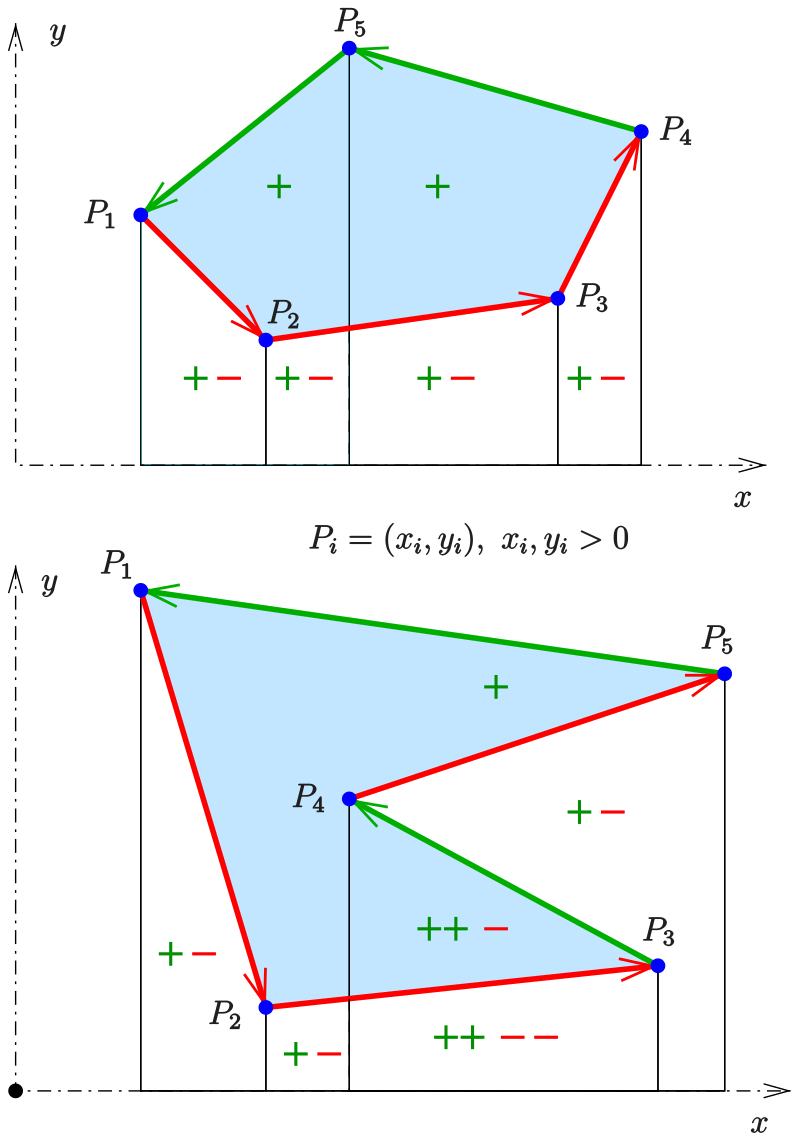
\includegraphics[width=6cm]{shoelace}
    \caption{Deriving the trapezoid formula. Source: Wikipediat{\tt/}shoelace formula.}
\end{figure}
In the 1st case the trapezoid is called {\it negative} in the 2nd case {\it positive}. The negative trapezoids delete those parts of positive trapezoids, which are outside the polygon. In case of a convex polygon (in the diagram the upper example) this is obvious: The polygon area is the sum of the areas of the positive trapezoids (green edges) minus the areas of the negative trapezoids (red edges). In the nonconvex case one has to consider the situation more carefully. In any case the result is
\begin{equation*}
    A= \sum_{i=1}^n A_i = \frac{1}{2}\sum_{i=1}^n (y_i + y_{i+1})(x_i - x_{i+1}).
\end{equation*}

%------------------------------------------------------------------------------%

\subsubsection{Triangle formula, determinant form -- Công thức tam giác, dạng định thức}
The triangle formula sums up the oriented areas $A_i$ of triangles $OP_iP_{i+1}$:
\begin{equation*}
    A = \frac{1}{2}\sum_{i=1}^n (x_iy_{i+1} - x_{i+1}y_i) = \frac{1}{2}\sum_{i=1}^n \begin{vmatrix}
        x_i & x_{i+1}\\y_i & y_{i+1}
    \end{vmatrix} = \frac{1}{2}\sum_{i=1}^n \begin{vmatrix}
        x_i & y_i\\x_{i+1} & y_{i+1}
    \end{vmatrix} = \frac{1}{2}(x_1y_2 - x_2y_1 + x_2y_3 - x_3y_2 + \cdots + x_ny_1 - x_1y_n).
\end{equation*}
Eliminating the brackets \& using $\sum_{i=1}^n x_iy_i = \sum_{i=1}^n x_{i+1}y_{i+1}$ (convention $P_{n+1} = P_1$), one gets the {\it determinant form} of the area formula:
\begin{equation*}
    A = \frac{1}{2}\sum_{i=1}^n (x_iy_{i+1} - x_{i+1}y_i) = \frac{1}{2}\sum_{i=1}^n \begin{vmatrix}
        x_i & x_{i+1}\\y_i & y_{i+1}
    \end{vmatrix}.
\end{equation*}
Because 1 half of the $i$th determinant is the oriented \href{https://en.wikipedia.org/wiki/Triangle_area}{area of the triangle} $\Delta OP_iP_{i+1}$ this version of the area formula is called {\it triangle form}.

-- Công thức tam giác tổng hợp các diện tích định hướng $A_i$ của các tam giác $OP_iP_{i+1}$:
\begin{equation*}
    A = \frac{1}{2}\sum_{i=1}^n (x_iy_{i+1} - x_{i+1}y_i) = \frac{1}{2}\sum_{i=1}^n \begin{vmatrix}
        x_i & x_{i+1}\\y_i & y_{i+1}
    \end{vmatrix} = \frac{1}{2}\sum_{i=1}^n \begin{vmatrix}
        x_i & y_i\\x_{i+1} & y_{i+1}
    \end{vmatrix} = \frac{1}{2}(x_1y_2 - x_2y_1 + x_2y_3 - x_3y_2 + \cdots + x_ny_1 - x_1y_n).
\end{equation*}
Loại bỏ dấu ngoặc \& sử dụng $\sum_{i=1}^n x_iy_i = \sum_{i=1}^n x_{i+1}y_{i+1}$ (quy ước $P_{n+1} = P_1$), ta sẽ có được {\it dạng định thức} của công thức diện tích:
\begin{equation*}
    A = \frac{1}{2}\sum_{i=1}^n (x_iy_{i+1} - x_{i+1}y_i) = \frac{1}{2}\sum_{i=1}^n \begin{vmatrix}
        x_i & x_{i+1}\\y_i & y_{i+1}
    \end{vmatrix}.
\end{equation*}
Vì 1 nửa của định thức $i$ là diện tích định hướng của tam giác $OP_iP_{i+1}$ nên phiên bản này của công thức diện tích được gọi là {\it dạng tam giác}.

%------------------------------------------------------------------------------%

\subsubsection{Shoelace formula -- Công thức dây giày}
The triangle formula is the base of the popular {\it shoelace formula}, which is a scheme that optimizes the calculation of the sum of the $2\times2$-determinants by hand:
\begin{equation*}
    2A = \begin{vmatrix}
        x_1 & x_2\\y_1 & y_2
    \end{vmatrix} + \begin{vmatrix}
        x_2 & x_3\\y_2 & y_3
    \end{vmatrix} + \cdots + \begin{vmatrix}
        x_n & x_1\\y_n & y_1
    \end{vmatrix} = \begin{vmatrix}
        x_1 & x_2 & x_3 & \cdots & x_n & x_1\\y_1 & y_2 & y_3 & \cdots & y_n & y_1\\
    \end{vmatrix}
\end{equation*}
Sometimes this determinant is transposed (written vertically, in 2 columns).

%------------------------------------------------------------------------------%

\subsubsection{Other formulas}

\begin{equation*}
    A = \frac{1}{2}\sum_{i=1}^n y_i(x_{i-1} - x_{i+1}) = \frac{1}{2}\left(y_1(x_n - x_2) + y_2(x_1 - x_3) + \cdots + y_n(x_{n-1} - x_1)\right) = \frac{1}{2}\sum_{i=1}^n x_i(y_{i+1} - y_{i-1}).
\end{equation*}
With $\sum_{i=1}^n x_iy_{i+1} = \sum_{i=1}^n x_{i-1}y_i$ (convention $P_0 = P_n,P_{n+1} = P_1$) one gets
\begin{equation*}
    2A = \sum_{i=1}^n (x_iy_{i+1} - x_{i+1}y_i) = \sum_{i=1}^n x_iy_{i+1} - \sum_{i=1}^n x_{i+1}y_i = \sum_{i=1}^n x_{i-1}y_i - \sum_{i=1}^n x_{i+1}y_i.
\end{equation*}
Combining both sums \& excluding $y_i$ leads to
\begin{equation*}
    A = \frac{1}{2}\sum_{i=1}^n y_i(x_{i-1} - x_{i+1}).
\end{equation*}
With the identity $\sum_{i=1}^n x_{i+1}y_i = \sum_{i=1}^n x_iy_{i-1}$ one gets
\begin{equation*}
    A = \frac{1}{2}\sum_{i=1}^n x_i(y_{i+1} - y_{i-1}).
\end{equation*}
Alternatively, this is a special case of Green's theorem with 1 function set to 0 \& the other set to $x$, s.t. the area is the integral of $x\,{\rm d}y$ along the boundary.

-- Với $\sum_{i=1}^n x_iy_{i+1} = \sum_{i=1}^n x_{i-1}y_i$ (quy ước $P_0 = P_n,P_{n+1} = P_1$) ta có
\begin{equation*}
    2A = \sum_{i=1}^n (x_iy_{i+1} - x_{i+1}y_i) = \sum_{i=1}^n x_iy_{i+1} - \sum_{i=1}^n x_{i+1}y_i = \sum_{i=1}^n x_{i-1}y_i - \sum_{i=1}^n x_{i+1}y_i.
\end{equation*}
Kết hợp cả 2 tổng \& loại trừ $y_i$ dẫn đến
\begin{equation*}
    A = \frac{1}{2}\sum_{i=1}^n y_i(x_{i-1} - x_{i+1}).
\end{equation*}
Với hằng đẳng thức $\sum_{i=1}^n x_{i+1}y_i = \sum_{i=1}^n x_iy_{i-1}$ ta có
\begin{equation*}
    A = \frac{1}{2}\sum_{i=1}^n x_i(y_{i+1} - y_{i-1}).
\end{equation*}
Ngoài ra, đây là trường hợp đặc biệt của định lý Green với 1 hàm được đặt thành 0 \& hàm còn lại được đặt thành $x$, s.t. diện tích là tích phân của $x\,{\rm d}y$ dọc theo biên.

%------------------------------------------------------------------------------%

\subsubsection{Exterior algebra -- Đại số ngoài}
A particularly concise statement of the formula can be given in terms of the exterior algebra. Let ${\bf v}_1,{\bf v}_2,\ldots,{\bf v}_n$ be the consecutive vertices of the polygon. The Cartesian coordinate expansion of the outer product w.r.t. the standard ordered orthonormal plane basis $({\bf x},{\bf y})$ gives ${\bf v}_i\land{\bf v}_{i+1} = (x_iy_{i+1} - x_{i+1}y_i){\bf x}\land{\bf y}$ \& the oriented area is given as follows:
\begin{equation*}
    A = \frac{1}{2}\sum_{i=1}^n {\bf v}_i\land{\bf v}_{i+1} = \frac{1}{2}\sum_{i=1}^n (x_iy_{i+1} - x_{i+1}y_i){\bf x}\land{\bf y}.
\end{equation*}
The area is given as a multiple of the unit area ${\bf x}\land{\bf y}$.

-- 1 phát biểu đặc biệt ngắn gọn về công thức có thể được đưa ra dưới dạng đại số ngoài. Giả sử ${\bf v}_1,{\bf v}_2,\ldots,{\bf v}_n$ là các đỉnh liên tiếp của đa giác. Khai triển tọa độ Descartes của tích ngoài w.r.t. cơ sở mặt phẳng chuẩn trực chuẩn sắp xếp $({\bf x},{\bf y})$ cho ${\bf v}_i\land{\bf v}_{i+1} = (x_iy_{i+1} - x_{i+1}y_i){\bf x}\land{\bf y}$ \& diện tích định hướng được đưa ra như sau:
\begin{equation*}
    A = \frac{1}{2}\sum_{i=1}^n {\bf v}_i\land{\bf v}_{i+1} = \frac{1}{2}\sum_{i=1}^n (x_iy_{i+1} - x_{i+1}y_i){\bf x}\land{\bf y}.
\end{equation*}
Diện tích được đưa ra dưới dạng bội số của diện tích đơn vị ${\bf x}\land{\bf y}$.

\begin{baitoan}[Area of polygon -- Diện tích đa giác]
    Viết thuật toán \& chương trình {\sf C{\tt/}C++, Pascal, Python} để tính diện tích của đa giác $n\in\mathbb{N},n\ge3$ đỉnh $A_1A_2\ldots A_n$ với tọa độ $n$ đỉnh $A_i(x_i,y_i)\in\mathbb{R}^2$ cho trước, $\forall i\in[n]$c.
    \item {\sf Input.} Dòng 1 chứa 1 số nguyên $n\in\mathbb{N},n\ge3$. Mỗi dòng trong $n$ dòng tiếp theo chứa 2 số thực $x_i,y_i\in\mathbb{R}$, $\forall i\in[n]$.
    \item {\sf Output.} In ra 1 số thực dương là diện tích của đa giác $A_1A_2\ldots A_n$.
\end{baitoan}

%------------------------------------------------------------------------------%

\subsection{Manipulations of a polygon -- Các thao tác trên 1 đa giác}
$A(P_1,\ldots,P_n)$ indicates the oriented area of the simple polygon $P_1,\ldots,P_n$ with $n\in\mathbb{N},n\ge4$. $A$ is positive{\tt/}negative if the orientation of the polygon is positive{\tt/}negative. From the triangle form of the area formula or the diagram below one observes for $i\in\overline{2,n-1}$:
\begin{equation*}
    A(P_1,\ldots,P_n) = A(P_1,\ldots,P_{i-1},P_{i+1},\ldots,P_n) + A(P_{i-1},P_i,P_{i+1}).
\end{equation*}
In case of $i = 1$ or $i = n$ one should 1st shift the indices. Hence:
\begin{enumerate}
    \item Moving $P_i$ affects only $A(P_{i-1},P_i,P_{i+1})$ \& leaves $A(P_1,\ldots,P_{i-1},P_{i+1},\ldots,P_n)$ unchanged. There is no change of the area if $P_i$ is moved parallel to $\overline{P_{i-1}P_{i+1}}$.
    \item Purging $P_i$ changes the total area by $A(P_{i-1},P_i,P_{i+1})$, which can be positive or negative.
    \item Inserting point $Q$ between $P_i,P_{i+1}$ changes the total area by $A(P_i,Q,P_{i+1})$, which can be positive or negative.
\end{enumerate}
-- $A(P_1,\ldots,P_n)$ biểu thị diện tích định hướng của đa giác đơn $P_1,\ldots,P_n$ với $n\in\mathbb{N},n\ge4$. $A$ là dương{\tt/}âm nếu định hướng của đa giác là dương{\tt/}âm. Từ dạng tam giác của công thức diện tích hoặc sơ đồ bên dưới, người ta quan sát thấy đối với $i\in\overline{2,n-1}$:
\begin{equation*}
    A(P_1,\ldots,P_n) = A(P_1,\ldots,P_{i-1},P_{i+1},\ldots,P_n) + A(P_{i-1},P_i,P_{i+1}).
\end{equation*}
Trong trường hợp $i = 1$ hoặc $i = n$, trước tiên người ta phải dịch chuyển các chỉ số. Do đó:
\begin{enumerate}
    \item Di chuyển $P_i$ chỉ ảnh hưởng đến $A(P_{i-1},P_i,P_{i+1})$ \& giữ nguyên $A(P_1,\ldots,P_{i-1},P_{i+1},\ldots,P_n)$. Không có thay đổi nào về diện tích nếu $P_i$ được di chuyển song song với $\overline{P_{i-1}P_{i+1}}$.
    \item Xóa $P_i$ làm thay đổi tổng diện tích theo $A(P_{i-1},P_i,P_{i+1})$, có thể dương hoặc âm.
    \item Chèn điểm $Q$ giữa $P_i,P_{i+1}$ làm thay đổi tổng diện tích theo $A(P_i,Q,P_{i+1})$, có thể dương hoặc âm.
\end{enumerate}


%------------------------------------------------------------------------------%

\subsection{Generalization of shoelace formula}
In higher dimensions the area of a polygon can be calculated from its vertices using the exterior algebra form of the Shoelace formula (e.g., in 3D, the sum of successive \href{https://en.wikipedia.org/wiki/Cross_product}{cross products}):
\begin{equation*}
    A = \frac{1}{2}\left\|\sum_{i=1}^n v_i\land v_{i+1}\right\|
\end{equation*}
(when the vertices are not \href{https://en.wikipedia.org/wiki/Coplanarity}{coplanar} this computes the \href{https://en.wikipedia.org/wiki/Vector_area}{vector area} enclosed by the loop, i.e., the \href{https://en.wikipedia.org/wiki/Projected_area}{projected area} or ``shadow'' in the plane in which it is greatest).

-- Ở các chiều cao hơn, diện tích của 1 đa giác có thể được tính từ các đỉnh của nó bằng cách sử dụng dạng đại số ngoài của công thức Shoelace (ví dụ, trong 3D, tổng của các tích có hướng liên tiếp):
\begin{equation*}
    A = \frac{1}{2}\left\|\sum_{i=1}^n v_i\land v_{i+1}\right\|
\end{equation*}
(khi các đỉnh không đồng phẳng, công thức này sẽ tính diện tích vectơ được bao quanh bởi vòng lặp, i.e., diện tích chiếu hoặc ``bóng'' trên mặt phẳng mà diện tích đó lớn nhất).

This formulation can also be generalized to calculate the volume of an $n$-dimensional polytope from the coordinates of its vertices, or more accurately, from its hypersurface mesh. E.g., the volume of a 3D polyhedron can be found by triangulating its surface mesh \& summing the signed volumes of the tetrahedra formed by each surface triangle \& the origin:
\begin{equation*}
    V = \frac{1}{6}\left\|\sum_F v_a\land v_b\land v_c\right\|
\end{equation*}
where the sum is over the faces \& care has to be taken to order the vertices consistently (all clockwise or anticlockwise viewed from outside the polyhedron). Alternatively, an expression in terms of the face areas \& surface normals may be derived using the divergence theorem.

-- Công thức này cũng có thể được khái quát hóa để tính thể tích của 1 đa diện $n$ chiều từ tọa độ các đỉnh của nó, hoặc chính xác hơn, từ lưới siêu bề mặt của nó. E.g., thể tích của 1 đa diện 3D có thể được tìm thấy bằng cách tam giác hóa lưới bề mặt của nó \& cộng các thể tích có dấu của tứ diện được tạo thành bởi mỗi tam giác bề mặt \& gốc:
\begin{equation*}
    V = \frac{1}{6}\left\|\sum_F v_a\land v_b\land v_c\right\|
\end{equation*}
trong đó tổng nằm trên các mặt \& phải cẩn thận để sắp xếp các đỉnh 1 cách nhất quán (tất cả theo chiều kim đồng hồ hoặc ngược chiều kim đồng hồ khi nhìn từ bên ngoài đa diện). Ngoài ra, 1 biểu thức theo diện tích mặt \& pháp tuyến bề mặt có thể được suy ra bằng cách sử dụng định lý phân kỳ.

%------------------------------------------------------------------------------%

\section{Problems: Computational elementary geometry}

\begin{baitoan}[Bao phủ hình chữ nhật nguyên 2D nhỏ nhất]
    {\rm(2.5 điểm)} Viết chương trình Python để tính chu vi, diện tích, \& độ dài đường chéo hình chữ nhật nhỏ nhất ``chứa trọn'' $n\in\mathbb{N}^\star$ điểm $A_1(x_1,y_1),A_2(x_2,y_2)$, $\ldots,A_n(x_n,y_n)\in\mathbb{R}^2$ với tọa độ nguyên $x_i,y_i\in\mathbb{Z}$, $\forall i = 1,\ldots,n$, cho trước trong mặt phẳng 2 chiều, ``chứa trọn'' ở đây nghĩa là các điểm chỉ được nằm bên trong hình chữ nhật, không được nằm trên cạnh hình chữ nhật.
    \item {\sf Input.} Dòng 1 chứa số nguyên $n\in\mathbb{N}^\star$:  * số điểm trong mặt phẳng 2 chiều. $n$ dòng tiếp theo, mỗi dòng chứa 2 số nguyên $x_i,y_i\in\mathbb{Z}$: hoành độ \& tung độ của điểm thứ $i$ $A_i(x_i,y_i)$.
    \item {\sf Output.} In ra chu vi, diện tích, \& đường chéo của hình chữ nhật thỏa mãn nhờ gọi lại hàm của Bài 1 (hoặc tự viết lại nếu muốn).
    \item {\sf Sample.}
    \begin{table}[H]
        \centering
        \begin{tabular}{|l|l|}
            \hline
            \verb|min_rectangle.inp| & \verb|min_rectangle.out| \\
            \hline
            4 & $P = 26$ \\
            1 0 & $S = 40$ \\
            -2 2 & $d = 9.43398113206$ \\
            -1 3 & \\
            4 2 & \\
            \hline
        \end{tabular}
    \end{table}
\end{baitoan}

\begin{proof}[Solution]
    Python:
    \begin{Verbatim}[numbers=left,xleftmargin=0mm]
        n = int(input()) # number of 2D points -- số điểm trên mặt phẳng
        x_min = y_min = 1e9
        x_max = y_max = -1e9
        for i in range(n):
        x, y = map(int, input().split())
        if x < x_min:
        x_min = x
        if x > x_max:
        x_max = x
        if y < y_min:
        y_min = y
        if y > y_max:
        y_max = y
        a, b = x_max - x_min + 2, y_max - y_min + 2
        print('P =', 2 * (a + b))
        print('S =', a * b)
        print('d =', sqrt(a * a + b * b))
    \end{Verbatim}
\end{proof}

\begin{baitoan}[Bao phủ hình hộp chữ nhật nguyên 3D nhỏ nhất]
    {\rm(3.5 điểm)} Viết chương trình Python để tính diện tích toàn phần, thể tích, \& độ dài đường chéo hình hộp chữ nhật nhỏ nhất chứa $n\in\mathbb{N}^\star$ điểm $A_1(x_1,y_1,z_1),A_2(x_2,y_2,z_2)$, $\ldots,A_n(x_n,y_n,z_n)\in\mathbb{R}^3$ với tọa độ nguyên $x_i,y_i\in\mathbb{Z}$, $\forall i = 1,\ldots,n$, cho trước trong không gian 3 chiều, ở đây các điểm có thể nằm bên trong hoặc nằm trên cạnh hình hộp chữ nhật.
    \item {\sf Input.} Dòng 1 chứa số nguyên $n\in\mathbb{N}^\star$: số điểm trong không gian 3 chiều. $n$ dòng tiếp theo, mỗi dòng chứa 3 số nguyên $x_i,y_i,z_i\in\mathbb{Z}$: hoành độ, tung độ, \& cao độ của điểm thứ $i$ $A_i(x_i,y_i,z_i)$.
    \item {\sf Output.} In ra diện tích toàn phần, thể tích, \& độ dài đường chéo hình hộp chữ nhật thỏa mãn, biết với hình hộp chữ nhật có kích thước $a\times b\times c$ thì $S_{\rm tp} = 2(ab + bc + ca),V = abc,d = \sqrt{a^2 + b^2 + c^2}$.
    \item {\sf Sample.}
    \begin{table}[H]
        \centering
        \begin{tabular}{|l|l|}
            \hline
            \verb|min_rectangular_cuboid.inp| & \verb|min_rectangular_cuboid.out| \\
            \hline
            4 & $S_{\rm tp} = 22$ \\
            1 0 0& $V = 6$ \\
            0 1 0 & $d = 3.74165738677 $ \\
            -1 0 2 & \\
            2 0 1 & \\
            \hline
        \end{tabular}
    \end{table}
\end{baitoan}

\begin{proof}[Solution]
    Python:
    \begin{Verbatim}[numbers=left,xleftmargin=0mm]
        n = int(input()) # number of 3D points
        x_min = y_min = z_min = 1e9
        x_max = y_max = z_max = -1e9
        for i in range(n):
        x, y, z = map(int, input().split())
        if x < x_min:
        x_min = x
        if x > x_max:
        x_max = x
        if y < y_min:
        y_min = y
        if y > y_max:
        y_max = y
        if z < z_min:
        z_min = z
        if z > z_max:
        z_max = z
        a, b, c = x_max - x_min, y_max - y_min, z_max - z_min
        print('S_tp =', 2 * (a * b + b * c + c * a))
        print('V =', a * b * c)
        print('d =', sqrt(a * a + b * b + c * c))
    \end{Verbatim}
\end{proof}

\begin{baitoan}[\cite{TL_chuyen_Tin_quyen_3}, 8.1, segment in triangle -- tìm độ dài đoạn thẳng nằm trong tam giác]
    Trên mặt phẳng cho $\Delta ABC$ \& đoạn thẳng $DE$. Tính độ dài của phần đoạn thẳng $DE$ nằm trong $\Delta ABC$.
    \item {\sf Input.} Dòng 1 có $6$ số thực $x_A,y_A,x_B,y_B,x_C,y_C$ lần lượt từng cặp là tọa độ tương ứng của 3 đỉnh $A,B,C$. Dòng 2 là $4$ số thực $x_D,y_D,x_E,y_E$ lần lượt từng cặp là tọa độ 2 điểm $D,E$.
    \item {\sf Output.} In 1 số thực duy nhất là độ dài phần đoạn thẳng $DE$ nằm trong $\Delta ABC$.
    \item {\sf Sample.}
    \begin{table}[H]
        \centering
        \begin{tabular}{|l|l|}
            \hline
            \verb|segment_in_triangle.inp| & \verb|segment_in_triangle.out| \\
            \hline
            0 2 2 4 4 2 & 3.16228 \\
            0 2 3 3 & \\
            \hline
        \end{tabular}
    \end{table}
\end{baitoan}

\begin{baitoan}[\cite{TL_chuyen_Tin_quyen_3}, 8.2, common area of 2 triangles -- tìm diện tích phần chung của 2 tam giác]
    Trên mặt phẳng cho $2$ tam giác. Tìm diện tích phần chung của $2$ tam giác.
    \item {\sf Input.} Gồm 2 dòng, mỗi dòng có $6$ số thực lần lượt từng cặp là tọa độ tương ứng của $3$ đỉnh của 1 tam giác. Các tọa độ có giá trị tuyệt đối $\le10^3$.
    \item {\sf Output.} In ra duy nhất 1 số thực là diện tích phần chung của 2 tam gaics này.
    \item {\sf Constraints.} $n\in[2\cdot10^5],m\in[100],x_i\in\{0,1,\ldots,m\}$.
    \item {\sf Sample.}
    \begin{table}[H]
        \centering
        \begin{tabular}{|l|l|}
            \hline
            \verb|common_area_triangle.inp| & \verb|common_area_triangle.out| \\
            \hline
            0 6 8 6 4 0 & 16 \\
            4 8 8 2 0 2 & \\
            \hline
        \end{tabular}
    \end{table}
\end{baitoan}

\begin{problem}[\href{https://cses.fi/problemset/task/2189}{CSES Problem Set{\tt/}point location test}]
    There is a line that goes through the points $p_1 = (x_1,y_2),p_2(x_2,y_2)$. There is also a point $p_3 = (x_3,y_3)$. Determine whether $p_3$ is located on the left or right side of the line or if it touches the line when we are looking from $p_1$ to $p_2$.
    \item {\sf Input.} The 1st input line has an integer $t\in\mathbb{N}^\star$: the number of tests. After this, there are $t$ lines that describe the tests. Each line has $6$ integers $x_1,y_1,x_2,y_2,x_3,y_3\in\mathbb{Z}$.
    \item {\sf Output.} For each test, print {\tt LEFT, RIGHT} or {\tt TOUCH}.
    \item {\sf Constraints.} $t\in[10^5],x_i,y_i\in\overline{-10^9,10^9}$, $\forall i\in[3]$, $x_1\ne x_2$ or $y_1\ne y_2$ (i.e., $(x_1,x_1)\ne(x_2,y_2)$).
    \item {\sf Sample.}
    \begin{table}[H]
        \centering
        \begin{tabular}{|l|l|}
            \hline
            \verb|point_location_test.inp| & \verb|point_location_test.out| \\
            \hline
            3 & LEFT \\
            1 1 5 3 2 3 0 2 & RIGHT \\
            1 1 5 3 4 1 & TOUCH \\
            1 1 5 3 3 2 & \\
            \hline
        \end{tabular}
    \end{table}
\end{problem}

\begin{proof}[Solution]
    C++ implementation:
    \begin{enumerate}
        \item PVT's C++ implementation: point location test
        \begin{Verbatim}[numbers=left,xleftmargin=0mm]
#include <bits/stdc++.h>
using namespace std;
#define ll long long

void solve() {
    ll x1, y1, x2, y2, x3, y3;
    cin >> x1 >> y1 >> x2 >> y2 >> x3 >> y3;
    ll dot = (x2 - x1) * (x3 - x1) + (y2 - y1) * (y3 - y1);
    ll det = (x2 - x1) * (y3 - y1) - (x3 - x1) * (y2 - y1);
    double angle = atan2(det, dot);
    if (angle == 0 || angle == M_PI || angle == -M_PI) cout << "TOUCH\n";
    else if (angle > 0) cout << "LEFT\n";
    else cout << "RIGHT\n";
}

int main() {
    ios_base::sync_with_stdio(false); cin.tie(NULL);
    ll t; cin >> t;
    while (t--)
    solve();
}
        \end{Verbatim}
        \item NHT's C++ implementation: point location test
        \begin{Verbatim}[numbers=left,xleftmargin=0mm]
#include <bits/stdc++.h>
#define ll long long
using namespace std;

int t;

int main() {
    ios_base::sync_with_stdio(false);
    cin.tie(nullptr);

    cin >> t;
    while (t--) {
        ll x1, y1, x2, y2, x3, y3;
        cin >> x1 >> y1 >> x2 >> y2 >> x3 >> y3;
        ll area = (x2 - x1) * (y3 - y1) - (y2 - y1) * (x3 - x1);
        if (area > 0)
        cout << "LEFT\n";
        else if (area < 0)
        cout << "RIGHT\n";
        else
        cout << "TOUCH\n";
    }
}
        \end{Verbatim}
    \end{enumerate}
\end{proof}

\begin{problem}[\href{https://cses.fi/problemset/task/2190}{CSES Problem Set{\tt/}line segment intersection}]
    There are $2$ line segments: the 1st goes through the points $(x_1,y_1),(x_2,y_2)$, \& the 2nd goes through the points $(x_3,y_3),(x_4,y_4)$. Determine if the line segments intersect, i.e., they have at least $1$ common point.
    \item {\sf Input.} The 1st input line has an integer $t\in\mathbb{N}^\star$: the number of tests. After this, there are $t$ lines that describe the tests. Each line has $8$ integers $x_1,y_1,x_2,y_2,x_3,y_3,x_4,y_4\in\mathbb{Z}$.
    \item {\sf Output.} For each test, print {\tt TEST} if the line segments intersect \& {\tt NO} otherwise.
    \item {\sf Constraints.} $t\in[10^5],x_i,y_i\in\overline{-10^9,10^9}$, $\forall i\in[4]$, $(x_1,x_1)\ne(x_2,y_2)$, $(x_3,x_3)\ne(x_4,y_4)$.
    \item {\sf Sample.}
    \begin{table}[H]
        \centering
        \begin{tabular}{|l|l|}
            \hline
            \verb|line_segment_intersection.inp| & \verb|line_segment_intersection.out| \\
            \hline
            5 & NO \\
            1 1 5 3 1 2 4 3 & YES \\
            1 1 5 3 1 1 4 3 & YES \\
            1 1 5 3 2 3 4 1 & YES \\
            1 1 5 3 2 4 4 1 & YES \\
            1 1 5 3 3 2 7 4 & \\
            \hline
        \end{tabular}
    \end{table}
\end{problem}

\begin{proof}[Solution]
    C++ implementation:
    \begin{enumerate}
        \item VNTA's C++ implementation: line segment intersection: \url{https://github.com/NQBH/advanced_STEM_beyond/blob/main/OLP_ICPC/C++/VNTA_line_segment_intersection.cpp}.
        \begin{Verbatim}[numbers=left,xleftmargin=0mm]
#include <bits/stdc++.h>
using namespace std;
#define ll long long

struct P {
    ll x;
    ll y;
};

int ori(P a, P b, P c) {
    ll v = (b.y - a.y) * (c.x - b.x) - (b.x - a.x) * (c.y - b.y);
    if (v == 0) return 0;
    return (v > 0) ? 1 : 2;
}

bool onSeg(P a, P b, P c) {
    return (b.x <= max(a.x, c.x) &&
    b.x >= min(a.x, c.x) &&
    b.y <= max(a.y, c.y) &&
    b.y >= min(a.y, c.y));
}

bool check(P a, P b, P c, P d) {
    int o1 = ori(a, b, c);
    int o2 = ori(a, b, d);
    int o3 = ori(c, d, a);
    int o4 = ori(c, d, b);

    if (o1 != o2 && o3 != o4) return true;

    if (o1 == 0 && onSeg(a, c, b)) return true;
    if (o2 == 0 && onSeg(a, d, b)) return true;
    if (o3 == 0 && onSeg(c, a, d)) return true;
    if (o4 == 0 && onSeg(c, b, d)) return true;

    return false;
}

int main() {
    ios::sync_with_stdio(0);
    cin.tie(0);

    int t; cin >> t;
    while (t--) {
        P p1, p2, p3, p4;
        cin >> p1.x >> p1.y >> p2.x >> p2.y >> p3.x >> p3.y >> p4.x >> p4.y;
        if (check(p1, p2, p3, p4)) cout << "YES\n";
        else cout << "NO\n";
    }
}
        \end{Verbatim}
    \end{enumerate}
\end{proof}

\begin{problem}[\href{https://cses.fi/problemset/task/2191}{CSES Problem Set{\tt/}polygon area}]
    Calculate the area of a given polygon. The polygon consists of $n$ vertices $(x_i,y_i)$, $\forall i\in[n]$. The vertices $(x_i,y_i)$ \& $(x_{i+1},y_{i+1})$ are adjacent for $i\in[n - 1]$, \& the vertices $(x_1,y_1)$ \& $(x_n,y_n)$ are also adjacent.
    \item {\sf Input.} The 1st input line has an integer $n\in\mathbb{N}^\star$: the number of vertices. After this, there are $n$ lines that describe the vertices. The $i$th such line has $2$ integers $x_i,y_i\in\mathbb{Z}$. You may assume that the polygon is simple, i.e., it does not intersect itself.
    \item {\sf Output.} Print $1$ integer: $2a\in\mathbb{Z}$ where the area of the polygon is $a$ (is ensures that the result is an integer).
    \item {\sf Constraints.} $n\in\overline{3,1000},x_i,y_i\in\overline{-10^9,10^9}$, $\forall i\in[n]$.
    \item {\sf Sample.}
    \begin{table}[H]
        \centering
        \begin{tabular}{|l|l|}
            \hline
            \verb|polygon_area.inp| & \verb|polygon_area.out| \\
            \hline
            4 & 16 \\
            1 1 & \\
            4 2 & \\
            3 5 & \\
            1 4 & \\
            \hline
        \end{tabular}
    \end{table}
\end{problem}

\begin{problem}[\href{https://cses.fi/problemset/task/2192}{CSES Problem Set{\tt/}point in polygon}]
    You are given a polygon of $n\in\mathbb{N}^\star$ vertices \& a list of $m\in\mathbb{N}^\star$ points. Determine for each point if it is inside, outside or on the boundary of the polygon. The polygon consists of $n$ vertices $(x_i,y_i)$, $\forall i\in[n]$. The vertices $(x_i,y_i)$ \& $(x_{i+1},y_{i+1})$ are adjacent for $i\in[n - 1]$, \& the vertices $(x_1,y_1)$ \& $(x_n,y_n)$ are also adjacent.
    \item {\sf Input.} The 1st input line has $2$ integer $n,m\in\mathbb{N}^\star$: the number of vertices in the polygon \& the number of points. After this, there are $n$ lines that describe the polygon. The $i$th such line has $2$ integers $x_i,y_i$. You may assume that the polygon is simple, i.e., it does not intersect itself. Finally, there are $m$ lines that describe the points. Each line has $2$ integers $x,y\in\mathbb{Z}$.
    \item {\sf Output.} For each point, print {\tt INSIDE, OUTSIDE} or {\tt BOUNDARY}.
    \item {\sf Constraints.} $M,n\in\overline{3,1000},m\in[1000],x,y,x_i,y_i\in\overline{-10^9,10^9}$, $\forall i\in[n]$.
    \item {\sf Sample.}
    \begin{table}[H]
        \centering
        \begin{tabular}{|l|l|}
            \hline
            \verb|point_in_polygon.inp| & \verb|point_in_polygon.out| \\
            \hline
            4 3 & INSIDE \\
            1 1 & OUTSIDE \\
            4 2 & BOUNDARY \\
            3 5 & \\
            1 4 & \\
            2 3 & \\
            3 1 & \\
            1 3 & \\
            \hline
        \end{tabular}
    \end{table}
\end{problem}

\begin{problem}[\href{https://cses.fi/problemset/task/2193}{CSES Problem Set{\tt/}polygon lattice points}]
    Given a polygon , calculate the number of lattice points inside the polygon \& on its boundary. A {\rm lattice point} is a point whose coordinates are integers. The polygon consists of $n\in\mathbb{N}^\star$ vertices $(x_i,y_i)$, $\forall i\in[n]$. The vertices $(x_i,y_i)$ \& $(x_{i+1},y_{i+1})$ are adjacent for $i\in[n - 1]$, \& the vertices $(x_1,y_1)$ \& $(x_n,y_n)$ are also adjacent.
    \item {\sf Input.} The 1st input line has an integer $n\in\mathbb{N}^\star$:  the number of vertices. After this, there are $n$ lines that describe the vertices. The $i$th such line has $2$ integers $x_i,y_i$. You may assume that the polygon is simple, i.e., it does not intersect itself.
    \item {\sf Output.} Print $2$ integers: the number of lattice points inside the polygon \& on its boundary.
    \item {\sf Constraints.} $n\in\overline{3,10^5},x_i,y_i\in\overline{-10^9,10^9}$, $\forall i\in[n]$.
    \item {\sf Sample.}
    \begin{table}[H]
        \centering
        \begin{tabular}{|l|l|}
            \hline
            \verb|polygon_lattice_point.inp| & \verb|polygon_lattice_point.out| \\
            \hline
            4 & 6 8 \\
            1 1 & \\
            5 3 & \\
            3 5 & \\
            1 4 & \\
            \hline
        \end{tabular}
    \end{table}
\end{problem}

\begin{problem}[\href{https://cses.fi/problemset/task/2194}{CSES Problem Set{\tt/}minimum Euclidean distance}]
    Given a set of points in 2D plane, find the minimum Euclidean distance between $2$ distinct points. The Euclidean distance of points $(x_1,y_1),(x_2,y_2)$ is $d((x_1,y_1),(x_2,y_2)) = \sqrt{(x_1 - x_2)^2 + (y_1 - y_2)^2}$.
    \item {\sf Input.} The 1st input line has an integer $n\in\mathbb{N}^\star$: the number of points. After this, there are $n$ lines that describe the points. Each line has $2$ integers $x,y\in\mathbb{Z}$: the coordinates of a point. You may assume that each point is distinct.
    \item {\sf Output.} Print $1$ integer: $d^2$ where $d$ is the minimum Euclidean distance (this ensures that the result is an integer).
    \item {\sf Constraints.} $n\in\overline{2,2\cdot10^5},x,y\in\overline{-10^9,10^9}$.
    \item {\sf Sample.}
    \begin{table}[H]
        \centering
        \begin{tabular}{|l|l|}
            \hline
            \verb|minimum_Euclidean_distance.inp| & \verb|minimum_Euclidean_distance.out| \\
            \hline
            4 & 2 \\
            2 1 & \\
            4 4 & \\
            1 2 & \\
            6 3 & \\
            \hline
        \end{tabular}
    \end{table}
\end{problem}

\begin{problem}[\href{https://cses.fi/problemset/task/2195}{CSES Problem Set{\tt/}convex hull}]
    Given a set of $n\in\mathbb{N}^\star$ points in the 2D plane, determine the convex hull of the points.
    \item {\sf Input.} The 1st input line has an integer $n\in\mathbb{N}^\star$: the number of points.  After this, there are $n$ lines that describe the points. Each line has $2$ integers $x,y\in\mathbb{Z}$: the coordinates of a point. You may assume that each point is distinct, \& the area of the hull is positive.
    \item {\sf Output.} 1st print an integer $k\in\mathbb{N}$: the number of points in the convex hull. After this, print $k$ lines that describe the points. You can print the points in any order. Print all points that lie on the convex hull.
    \item {\sf Constraints.} $n\in\overline{3,2\cdot10^5},x,y\in\overline{-10^9,10^9}$.
    \item {\sf Sample.}
    \begin{table}[H]
        \centering
        \begin{tabular}{|l|l|}
            \hline
            \verb|.inp| & \verb|.out| \\
            \hline
            6 & 4 \\
            2 1 & 2 1 \\
            2 5 & 2 5 \\
            3 3 & 4 4 \\
            4 3 & 6 3 \\
            4 4 & \\
            6 3 & \\
            \hline
        \end{tabular}
    \end{table}
\end{problem}

\begin{problem}[\href{https://cses.fi/problemset/task/3410}{CSES Problem Set{\tt/}maximum Manhattan distance}]
    A set is initially empty \& $n\in\mathbb{N}^\star$ points are added to it. Calculate the maximum Manhattan distance of $2$ points after each addition.
    \item {\sf Input.} The 1st input line has an integer $n\in\mathbb{N}^\star$: the number of points. The following $n$ lines describe the points. Each line has $2$ integers $x,y\in\mathbb{Z}$. You can assume that each point is distinct.
    \item {\sf Output.} After each addition, print the maximum distance.
    \item {\sf Constraints.} $n\in\overline{2,2\cdot10^5},x,y\in\overline{-10^9,10^9}$.
    \item {\sf Sample.}
    \begin{table}[H]
        \centering
        \begin{tabular}{|l|l|}
            \hline
            \verb|maximum_Manhattan_distance.inp| & \verb|maximum_Manhattan_distance.out| \\
            \hline
            5 & 0 \\
            1 1 & 3 \\
            3 2 & 4 \\
            2 4 & 4 \\
            2 1 & 7 \\
            4 5 & \\
            \hline
        \end{tabular}
    \end{table}
\end{problem}

\begin{problem}[\href{https://cses.fi/problemset/task/3411}{CSES Problem Set{\tt/}all Manhattan distances}]
    Given a set of points, calculate the sum of all Manhattan distances between $2$ point pairs.
    \item {\sf Input.} The 1st input line has an integer $n\in\mathbb{N}^\star$: the number of points. The following $n$ lines describe the points. Each line has $2$ integers $x,y\in\mathbb{Z}$. You can assume that each point is distinct.
    \item {\sf Output.} Print the sum of all Manhattan distances.
    \item {\sf Constraints.} $n\in\overline{2,2\cdot10^5},x,y\in\overline{-10^9,10^9}$.
    \item {\sf Sample.}
    \begin{table}[H]
        \centering
        \begin{tabular}{|l|l|}
            \hline
            \verb|all_Manhattan_distance.inp| & \verb|all_Manhattan_distance.out| \\
            \hline
            5 & 36 \\
            1 1 & \\
            3 2 & \\
            2 4 & \\
            2 1 & \\
            4 5 & \\
            \hline
        \end{tabular}
    \end{table}
\end{problem}

\begin{problem}[\href{https://cses.fi/problemset/task/1740}{CSES Problem Set{\tt/}intersection points}]
    Given $n\in\mathbb{N}^\star$ horizontal \& vertical line segments, calculate the number of their intersection points. You can assume that no parallel line segments intersect, \& no endpoint of a line segment is an intersection point.
    \item {\sf Input.} The 1st input line has an integer $n\in\mathbb{N}^\star$: the number of line segments. Then there are $n$ lines describing the line segments. Each line has $4$ integers: $x_1,y_1,x_2,y_2$: a line segment begins at point $(x_1,y_1)$ \& ends at point $(x_2,y_2)$.
    \item {\sf Output.} Print the number of intersection points.
    \item {\sf Constraints.} $n\in[10^5],x_1,x_2,y_1,y_2\in\overline{-10^6,10^6}$, $(x_1,y_1)\ne(x_2,y_2)$.
    \item {\sf Sample.}
    \begin{table}[H]
        \centering
        \begin{tabular}{|l|l|}
            \hline
            \verb|intersection_point.inp| & \verb|intersection_point.out| \\
            \hline
            3 & 2 \\
            2 3 7 3 & \\
            3 1 3 5 & \\
            6 2 6 6 & \\
            \hline
        \end{tabular}
    \end{table}
\end{problem}

\begin{problem}[\href{https://cses.fi/problemset/task/3427}{CSES Problem Set{\tt/}line segments trace I}]
    There are $n\in\mathbb{N}^\star$ line segments whose endpoints have integer coordinates. The left $x$-coordinate of each segment is $0$ \& the right $x$-coordinate is $m\in\mathbb{N}^\star$. The slope of each segment is an integer. For each $x$-coordinate $0,1,\ldots,m$, find the maximum point in any line segment.
    \item {\sf Input.} The 1st input line has $2$ integer $n,m\in\mathbb{N}^\star$: the number of line segments \& the maximum $x$-coordinate. The next $n$ lines describe the line segments. Each line has $2$ integers $y_1,y_2$: there is a line segment between points $(0,y_1)$ \& $(m,y_2)$.
    \item {\sf Output.} Print $m + 1$ integers: the maximum points for $x = 0,1,\ldots,m$.
    \item {\sf Constraints.} $m,n\in[10^5],m\in[100],y_1,y_2\in\overline{0,10^9}$.
    \item {\sf Sample.}
    \begin{table}[H]
        \centering
        \begin{tabular}{|l|l|}
            \hline
            \verb|line_segment_trace_I.inp| & \verb|line_segment_trace_I.out| \\
            \hline
            4 5 & 10 8 6 5 5 6 \\
            1 6 & \\
            7 2 & \\
            5 5 & \\
            10 0 & \\
            \hline
        \end{tabular}
    \end{table}
\end{problem}

\begin{problem}[\href{https://cses.fi/problemset/task/3428}{CSES Problem Set{\tt/}line segments trace II}]
    There are $n\in\mathbb{N}^\star$ line segments whose endpoints have integer coordinates. Each $x$-coordinate is between $0$ \& $m$. The slope of each segment is an integer. For each $x$-coordinate $0,1,\ldots,m$, find the maximum point in any line segment. If there is no segment at some point, the maximum is $-1$.
    \item {\sf Input.} The 1st input line has $2$ integers $n,m\in\mathbb{N}^\star$: the number  of line segments \& the maximum $x$-coordinate. The next $n$ lines describe the line segments. Each line has $4$ integers $x_1,y_1,x_2,y_2$: there is a line segment between points $(x_1,y_1),(x_2,y_2)$.
    \item {\sf Output.} Print $m + 1$ integers: the maximum points for $x = 0,1,\ldots,m$.
    \item {\sf Constraints.} $m,n\in[10^5],0\le x_1 < x_2\le m,y_1,y_2\in\overline{0,10^9}$.
    \item {\sf Sample.}
    \begin{table}[H]
        \centering
        \begin{tabular}{|l|l|}
            \hline
            \verb|line_segment_trace_II.inp| & \verb|line_segment_trace_II.out| \\
            \hline
            4 5 & -1 2 8 6 6 7 \\
            1 1 3 3 & \\
            1 2 4 2 & \\
            2 4 5 7 & \\
            2 8 5 2 & \\
            \hline
        \end{tabular}
    \end{table}
\end{problem}

\begin{problem}[\href{https://cses.fi/problemset/task/3429}{CSES Problem Set{\tt/}lines \& queries I}]
    Efficiently process the following types of queries:
    \begin{enumerate}
        \item Add a line $ax + b$.
        \item Find the maximum point in any line at position $x$.
    \end{enumerate}
    \item {\sf Input.} The 1st input line has an integer $n\in\mathbb{N}^\star$: the number of queries. The following $n$ lines describe the queries. The format of each line is either {\tt1 a b} or {\tt2 x}. You may assume that the 1st query is of type 1.
    \item {\sf Output.} Print the answer for each query of type 2.
    \item {\sf Constraints.} $n\in[2\cdot10^5],a,b\in\overline{-10^9,10^9},x\in\overline{0,10^5}$.
    \item {\sf Sample.}
    \begin{table}[H]
        \centering
        \begin{tabular}{|l|l|}
            \hline
            \verb|line_query_I.inp| & \verb|line_query_I.out| \\
            \hline
            6 & 3 \\
            1 1 2 & 5 \\
            2 1 & 4 \\
            2 3 & 5 \\
            1 0 4 & \\
            2 1 & \\
            2 3 & \\
            \hline
        \end{tabular}
    \end{table}
\end{problem}

\begin{problem}[\href{https://cses.fi/problemset/task/3430}{CSES Problem Set{\tt/}lines \& queries II}]
    Efficiently process the following types of queries:
    \begin{enumerate}
        \item Add a line $ax + b$ that is active in range $[l,r]$.
        \item Find the maximum point in any active line at position $x$.
    \end{enumerate}
    \item {\sf Input.} The 1st input line has an integer $n\in\mathbb{N}^\star$: the number of queries. The following $n$ lines describe the queries. The format of each line is either {\tt1 a b l r} or {\tt2 x}.
    \item {\sf Output.} Print the answer for each query of type 2. If no line is active, print {\tt NO}.
    \item {\sf Constraints.} $n\in[2\cdot10^5],a,b\in\overline{-10^9,10^9},x,l,r\in\overline{0,10^5}$.
    \item {\sf Sample.}
    \begin{table}[H]
        \centering
        \begin{tabular}{|l|l|}
            \hline
            \verb|line_query_II.inp| & \verb|line_query_II.out| \\
            \hline
            6 & 5 \\
            1 1 2 1 3 & NO \\
            2 3 & 5 \\
            2 4 & 4 \\
            1 0 4 1 5 & \\
            2 3 & \\
            2 4 & \\
            \hline
        \end{tabular}
    \end{table}
\end{problem}

\begin{problem}[\href{https://cses.fi/problemset/task/1741}{CSES Problem Set{\tt/}area of rectangles}]
    Given $n\in\mathbb{N}^\star$, determine the total area of their union.
    \item {\sf Input.} The 1st input line has an integer $n\in\mathbb{N}^\star$: the number of rectangles. After that, there are $n$ lines describing the rectangles. Each line has $4$ integers $x_1,y_1,x_2,y_2$: a rectangle begins at point $(x_1,y_1)$ \& ends at point $(x_2,y_2)$.
    \item {\sf Output.} Print the total area covered by the rectangles.
    \item {\sf Constraints.} $n\in[10^5],m\in[100],x_1,x_2,y_1,y_2\in\overline{-10^6,10^6}$.
    \item {\sf Sample.}
    \begin{table}[H]
        \centering
        \begin{tabular}{|l|l|}
            \hline
            \verb|area_rectangle.inp| & \verb|area_rectangle.out| \\
            \hline
            3 & 24 \\
            1 3 4 5 & \\
            3 1 7 4 & \\
            5 3 8 6 & \\
            \hline
        \end{tabular}
    \end{table}
\end{problem}

\begin{problem}[\href{https://cses.fi/problemset/task/1742}{CSES Problem Set{\tt/}robot path}]
    You are given a description of a robot's path. The robot begins at point $(0,0)$ \& performs $n\in\mathbb{N}^\star$ commands. Each command moves the robot some distance up, down, left, or right. The robot will stop when it has performed all commands, or immediately when it returns to a point that it has already visited. Calculate the total distance the robot moves.
    \item {\sf Input.} The 1st input line has an integer $n\in\mathbb{N}^\star$: the number of commands. After that, there are $n$ lines describing the commands. each line has a character $d$ \& an integer $x\in\mathbb{N}^\star$: the robot moves the distance $x$ to the direction $d$. Each direction is {\tt U, D, L, R} (up, down, left, right).
    \item {\sf Output.} Print the total distance the robot moves.
    \item {\sf Constraints.} $n\in[10^5],x\in[10^6]$.
    \item {\sf Sample.}
    \begin{table}[H]
        \centering
        \begin{tabular}{|l|l|}
            \hline
            \verb|robot_path.inp| & \verb|robot_path.out| \\
            \hline
            5 & 9 \\
            U 2 & \\
            R 3 & \\
            D 1 & \\
            L 5 & \\
            U 2 & \\
            \hline
        \end{tabular}
    \end{table}
\end{problem}

\begin{problem}[IMO2007P6]
    Let $n\in\mathbb{N}^\star$. Consider $S = \{(x,y,z);x,y,z\in\overline{0,n},\ x + y + z > 0\}$ as a set of $(n + 1)^3 - 1$ points in 3D space. Determine the smallest possible number of planes, the union of which contains $S$ but does not include $(0,0,0)$.
\end{problem}

\begin{baitoan}[\cite{Vinh_Lu_Olympic_Toan}, 6., p. 10, IMO2007P6]
    Cho $n\in\mathbb{N}^\star$. Xét $S = \{(x,y,z);x,y,z\in\overline{0,n},\ x + y + z > 0\}$ là 1 tập hợp gồm $(n + 1)^3 - 1$ điểm trong không gian $3$-chiều. Xác định số nhỏ nhất có thể các mặt phẳng mà hợp của chúng chứa tất cả các điểm của $S$ nhưng không chứa điểm $(0,0,0)$.
\end{baitoan}

%------------------------------------------------------------------------------%

\chapter{Number Theory -- Lý Thuyết Số}
\minitoc

%------------------------------------------------------------------------------%

\section{Divisor -- Ước Số}

\begin{problem}[IMO2007P5]
    Let $a,b\in\mathbb{N}^\star$. Show that if $4ab - 1|(4a^2 - 1)^2$, then $a = b$.
\end{problem}

\begin{baitoan}[CP version of IMO2007P5]
    Cho $m,n\in\mathbb{N}^\star$. Đếm số phần tử của tập hợp
    \begin{equation*}
        S = \{(a,b)\in[m]\times[n];4ab - 1|(4a^2 - 1)^2\} = \{(a,b)\in[m]\times[n];(4a^2 - 1)^2\divby4ab - 1\}.
    \end{equation*}
    \item {\sf Input.} Chỉ 1 dòng chứa $m,n\in\mathbb{N}^\star$.
    \item {\sf Output}. $|S|$.
    \item {\sf Sample.}
    \begin{table}[H]
        \centering
        \begin{tabular}{|l|l|}
            \hline
            \verb|IMO2007_P5.inp| & \verb|IMO2007_P5.out| \\
            \hline
            5 3 & 3 \\
            \hline
            10 15 & 10 \\
            \hline
        \end{tabular}
    \end{table}
\end{baitoan}

\begin{proof}[Solution]
    Theo lời giải bài toán IMO2007P5 trước đó, đáp số bài toán này đơn giản chỉ là $\min\{m,n\}$. Nhưng đó là về mặt chứng minh toán học, sau đây ta sẽ dùng vòng lặp để kiểm tra.

    C++ implementation:
    \begin{enumerate}
        \item DPAK's C++ implementation: IMO2007P5:
        \begin{Verbatim}[numbers=left,xleftmargin=0mm]
#include <iostream>
using namespace std;
int m, n;
const double oo = 1e9 + 7;

int main() {
    cin >> m >> n;
    int cnt = 0;
    for (int a = 1; a <= m; ++a) {
        int num = 4 * a * a - 1;
        num = num * num;
        for (int b = 1; b <= n; ++b) {
            int divisor = 4 * a * b - 1;
            if (num % divisor == 0) ++cnt;
        }
    }
    cout << cnt;
}
        \end{Verbatim}

        \item TQS's \& DNDK's C++ implementation: IMO2007P5:
        \begin{Verbatim}[numbers=left,xleftmargin=0mm]
#include <iostream>
using namespace std;

int main() {
    int m, n, count = 0;
    cin >> m >> n;
    for (int i = 1; i <= m; ++i)
        for (int j = 1; j <= n; ++j)
            if (((4 * i * i - 1) * (4 * i * i - 1)) % (4 * i * j - 1) == 0) ++count;
    cout << count;
}
        \end{Verbatim}

        \begin{remark}
            Dù code này không cần dùng tới 2 biến phụ {\tt num, divisor} như code của DPAK, nhưng sẽ tính nhiều lần hơn do đoạn code {\tt(4 * i * i - 1) * (4 * i * i - 1)} lặp lại phép tính {\tt(4 * i * i - 1)} 2 lần (unnecessary duplication).
        \end{remark}


    \end{enumerate}

\end{proof}

\begin{problem}[IMO2008P3]
    Prove that there exists infinitely many positive integers $n$ s.t. $n^2 + 1$ has a prime divisor which is $> 2n + \sqrt{2n}$.
\end{problem}

\begin{baitoan}[\cite{Vinh_Lu_Olympic_Toan}, p. 12, IMO2008P3]
    Chứng minh tồn tại vô hạn $n\in\mathbb{N}^\star$ sao cho $n^2 + 1$ có ước nguyên tố lớn hơn $2n + \sqrt{2n}$.
\end{baitoan}

\begin{baitoan}[CP version of IMO2008P3]
    Đếm số số $n\in\mathbb{N}^\star$ sao cho $n^2 + 1$ có ước nguyên tố lớn hơn $2n + \sqrt{2n}$ trong phạm vi $n\in[a,b]$ với $a,b\in\mathbb{N}^\star$ cho trước.
    \item {\sf Input.} 2 số $a,b\in\mathbb{N}^\star$.
    \item {\sf Output.} Số số $n\in[a,b]$ thỏa mãn.
\end{baitoan}

\begin{proof}[Solution]


    C++ implementation:
    \begin{enumerate}
        \item DPAK's C++ implementation: IMO2008P3:
        \begin{Verbatim}[numbers=left,xleftmargin=0mm]
#include <iostream>
#include <cmath>
using namespace std;
long long a, b;
const double oo = 1e9 + 7;

int main() {
    long long cnt = 0;
    cin >> a >> b;
    for (long long i = a; i <= b; ++i) {
        long long new_num = i * i + 1;
        double limit = 2.0 * i + sqrt(2 * i);
        long long temp = new_num;
        bool ok = false;
        for (long long j = 2; j * j <= new_num; ++j)
        if (temp % j == 0) {
            while (temp % j == 0) temp /= j;
            if (j > limit) {
                ok = true;
                break;
            }
        }
        if (!ok && temp > 1 && temp > limit) ok = true;
        if (ok) ++cnt;
    }
    cout << cnt;
}
        \end{Verbatim}

        \item DNDK's C++ implementation: IMO2008P3:
        \begin{Verbatim}[numbers=left,xleftmargin=0mm]
#include <iostream>
#include <cmath>
using namespace std;

bool check(long long n) {
    long long x = n * n + 1, X = x;
    long long y = 2 * n + sqrtl(2 * n);
    for (long long i = 2; i * i <= X; ++i)
        if (x % i == 0) {
            while (x % i == 0) x /= i;
            if (i > y) return true;
        }
    if (x > 1 and x > y) return true;
    return false;
}

int main() {
    long long a, b;
    cin >> a >> b;
    long long count = 0;
    for (long long i = a; i <= b; ++i)
        if (check(i)) ++count;
    cout << count;
}
        \end{Verbatim}
    \end{enumerate}
\end{proof}

\begin{problem}[IMO2011P1]
    Given any set $A = \{a_1,a_2,a_3,a_4\}$ of $4$ distinct positive integers, we denote $s_A\coloneqq a_1 + a_2 + a_3 + a_4$. Let $n_A$ denote the number of pairs $(i,j)$ with $1\le i < j\le4$ for which $a_i + a_j|s_A$. Find all sets $A$ of $4$ distinct positive integers which achieve the largest possible value of $n_A$.
\end{problem}

\begin{baitoan}[\cite{Vinh_Lu_Olympic_Toan}, 1., p. 17, IMO2011P1]
    Cho tập hợp $A = \{a_1,a_2,a_3,a_4\}$ gồm $4$ số nguyên phân biệt, ta ký hiệu tổng $a_1 + a_2 + a_3 + a_4$ bởi $s_A$. Giả sử $n_A$ là số các cặp $(i,j)$ với $1\le i < j\le4$ sao cho $a_i + a_j\divby s_A$. Tìm tất cả các tập hợp $A$ gồm $4$ số nguyên dương phân biệt mà với chúng $n_A$ đạt được {\rm GTLN} có thể.
\end{baitoan}

\begin{baitoan}
    Viết thuật toán \& chương trình {\sf C{\tt/}C++, Pascal, Python} để minh hoạ IMO2011P1.
\end{baitoan}

%------------------------------------------------------------------------------%

\section{$p$-adic valuation -- Đánh giá $p$-adic}
\textbf{\textsf{Resources -- Tài nguyên.}}
\begin{enumerate}
    \item \href{https://en.wikipedia.org/wiki/P-adic_valuation}{Wikipedia{\tt/}$p$-adic valuation}.
\end{enumerate}
In number theory, the {\it$p$-adic valuation} or {\it$p$-adic order} of an integer $n$ is the exponent of the highest power of the prime number $p$ that divides $n$, denoted by $\nu_p(n)$. Equivalently, $\nu_p(n)$ is the exponent to which $p$ appears in the prime factorization of $n$.

-- Trong lý thuyết số, {\it$p$-adic evaluation} hoặc {\it$p$-adic order} của 1 số nguyên $n$ là số mũ của lũy thừa cao nhất của số nguyên tố $p$ chia hết cho $n$, được ký hiệu là $\nu_p(n)$. Tương đương, $\nu_p(n)$ là số mũ mà $p$ xuất hiện trong phép phân tích thừa số nguyên tố của $n$.
\begin{equation*}
    n\divby p^{\nu_p(n)},\ n\not{\divby p^{\nu_p(n) + 1}},\ \forall n\in\mathbb{N}^\star,\ \forall p\mbox{ is prime}.
\end{equation*}

\begin{definition}[$p$-adic valuatiion]
    Let $p$ be a prime number. The {\rm$p$-adic valuation} of $n\in\mathbb{Z}$ is defined by
    \begin{equation*}
        \nu_p(n) = \left\{\begin{split}
            &\max\{k\in\mathbb{N};p^k|n\}&&\mbox{if } n\ne0,\\
            &\infty&&\mbox{if } n = 0.
        \end{split}\right.
    \end{equation*}
    In particular, $\nu_p$ is a function $\nu_p:\mathbb{Z}\to\mathbb{N}\cup\{\infty\}$. The $p$-adic valuation can be extended to the rational numbers as the function $\nu_p:\mathbb{Q}\to\mathbb{Z}\cup\{\infty\}$ defined by $\nu_p\left(\frac{r}{s}\right) = \nu_p(r) - \nu_p(s)$.
\end{definition}

\begin{example}
    (a) $|-12| = 12 = 2^2\cdot3^1\cdot5^0\Rightarrow\nu_2(-12) = \nu_2(12) = 2,\nu_3(-12) = \nu_3(12) = 1,\nu_p(-12) = \nu_p(12) = 0$, $\forall$ prime $p\ge5$. (b) $\frac{9}{8} = 2^{-3}\cdot3^2\Rightarrow\nu_2\left(\pm\frac{9}{8}\right) = -3,\nu_3\left(\pm\frac{9}{8}\right) = 2$.
\end{example}
The notation $p^k||n$ is sometimes used to mean $k = \nu_p(n)$. One has
\begin{equation*}
    n\divby p^{\nu_p(n)}\Rightarrow n\ge p^{\nu_p(n)}\Rightarrow\nu_p(n)\le\log_pn,\ \forall n\in\mathbb{N}^\star.
\end{equation*}

\begin{lemma}[Some properties of $p$-adic valuation]
    (i) $\nu_p(rs) = \nu_p(r) + \nu_p(s)$. (ii) $\nu_p(r + s) = \min\{\nu_p(r),\nu_p(s)\}$.
    \item(iii) {\rm(Legendre's formula)} $\nu_p(n!) = \sum_{i=1}^\infty \left\lfloor\dfrac{n}{p^i}\right\rfloor = \sum_{i=1}^{\lfloor\log_pn\rfloor} \left\lfloor\dfrac{n}{p^i}\right\rfloor$, $\forall n\in\mathbb{N}$.
    \item(iv)
    \begin{equation*}
        \nu_p(n) = \nu_p(n!) - \nu_p((n - 1)!) = \sum_{i=1}^\infty \left(\left\lfloor\frac{n}{p^i}\right\rfloor - \left\lfloor\frac{n - 1}{p^i}\right\rfloor\right) = \sum_{i=1}^{\lfloor\log_pn\rfloor} \left(\left\lfloor\frac{n}{p^i}\right\rfloor - \left\lfloor\frac{n - 1}{p^i}\right\rfloor\right),\ \forall n\in\mathbb{N}.
    \end{equation*}
    This formula can be extended to negative integer values
    \begin{equation*}
        \nu_p(n) = \sum_{i=1}^{\lfloor\log_p|n|\rfloor} \left(\left\lfloor\frac{|n|}{p^i}\right\rfloor - \left\lfloor\frac{|n| - 1}{p^i}\right\rfloor\right),\ \forall n\in\mathbb{Z}.
    \end{equation*}
\end{lemma}

%------------------------------------------------------------------------------%

\subsection{$p$-adic absolute value}

\begin{definition}[$p$-adic absolute value]
    The {\rm$p$-adic absolute value} (or {\rm$p$-adic norm}, though not a form in the sense of analysis) on $\mathbb{Q}$ is the function $|\cdot|_p:\mathbb{Q}\to[0,\infty)$ defined by $|r|_p = p^{-\nu_p(r)}$.
\end{definition}

\begin{dinhnghia}[Giá trị tuyệt đối $p$-adic]
    Giá trị tuyệt đối {\rm$p$-adic} (hoặc {\rm$p$-adic norm}, mặc dù không phải là 1 dạng theo nghĩa phân tích) trên $\mathbb{Q}$ là hàm $|\cdot|_p:\mathbb{Q}\to[0,\infty)$ được xác định bởi $|r|_p = p^{-\nu_p(r)}$.
\end{dinhnghia}

\begin{example}
    (a) $|0|_p = p^{-\infty} = 0$, $\forall p$ prime. (b) $|-12|_2 = 2^{-2} = \frac{1}{4}$. (c) $\left|\frac{9}{8}\right|_2 = 2^{-(-3)} = 8$.
\end{example}

\begin{lemma}[Some properties of $p$-adic absolute value]
    The $p$-adic absolute value satisfies the following properties:
    \item(i) Nonnegativity: $|r|_p\ge0$.
    \item(ii) $|r|_p = 0\Leftrightarrow r = 0$.
    \item(iii) $|rs|_p = |r|_p|s|_p$.
    \item(iv) \href{https://en.wikipedia.org/wiki/Ultrametric_space}{Non-Archimedean}: $|r + s|_p\le\max\{|r|_p,|s|_p\}$.
\end{lemma}
From the multiplicativity $|rs|_p = |r|_p|s|_p$ it follows that $|1|_p = 1 = |-1|_p$ for the roots of unity $\pm1$ \& consequently also $|-r|_p = |r|_p$. The subadditivity $|r + s|_p\le|r|_p + |s|_p$ follows from the non-Archimedean triangle inequality $|r + s|_p\le\max(|r|_p,|s|_p)$.

-- Từ phép nhân $|rs|_p = |r|_p|s|_p$ suy ra $|1|_p = 1 = |-1|_p$ đối với các căn bậc 2 của đơn vị $\pm1$ \& do đó cũng $|-r|_p = |r|_p$. Phép nhân dưới $|r + s|_p\le|r|_p + |s|_p$ suy ra từ bất đẳng thức tam giác không phải Archimedean $|r + s|_p\le\max(|r|_p,|s|_p)$.

The choice of base $p$ in the exponentiation $p^{-\nu_p(r)}$ makes no difference for most of the properties, but supports the product formula: $\prod_{0,p} |r|_p = 1$ where the product is taken over all primes $p$ \& the usual absolute value, denoted $|r|_0$. This follows from simply taking the \href{https://en.wikipedia.org/wiki/Prime_factorization}{prime factorization}: each prime power factor $p^k$ contributes its reciprocal to its $p$-adic absolute value, \& then the usual Archimedean absolute value cancels all of them.

-- Việc lựa chọn cơ số $p$ trong phép lũy thừa $p^{-\nu_p(r)}$ không tạo ra sự khác biệt đối với hầu hết các tính chất, nhưng hỗ trợ công thức tích: $\prod_{0,p} |r|_p = 1$ trong đó tích được lấy trên tất cả các số nguyên tố $p$ \& giá trị tuyệt đối thông thường, được ký hiệu là $|r|_0$. Điều này tuân theo cách đơn giản là lấy thừa số nguyên tố: mỗi thừa số nguyên tố $p^k$ đóng góp nghịch đảo của nó vào giá trị tuyệt đối $p$-adic của nó, \& sau đó giá trị tuyệt đối Archimedean thông thường sẽ hủy bỏ tất cả chúng.

A metric space can be formed on the set $\mathbb{Q}$ with a (non-Archimedean, \href{https://en.wikipedia.org/wiki/Translation_invariance}{translation-invariant}) metric $d:\mathbb{Q}\times\mathbb{Q}\to[0,\infty)$ defined by $d(r,s) = |r - s|_p$. The completion of $\mathbb{Q}$ w.r.t. this metric leads to the set $\mathbb{Q}_p$ of $p$-adic numbers.

-- 1 không gian metric có thể được hình thành trên tập $\mathbb{Q}$ với 1 metric (không phải Archimedean, bất biến tịnh tiến) $d:\mathbb{Q}\times\mathbb{Q}\to[0,\infty)$ được xác định bởi $d(r,s) = |r - s|_p$. Sự hoàn thành của $\mathbb{Q}$ đối với metric này dẫn đến tập $\mathbb{Q}_p$ của các số $p$-adic.

%------------------------------------------------------------------------------%

\subsection{Finding power of factorial divisor -- Tìm lũy thừa của ước số giai thừa}
\textbf{\textsf{Resources -- Tài nguyên.}}
\begin{enumerate}
    \item \href{https://cp-algorithms.com/algebra/factorial-divisors.html}{Algorithms for Competitive Programming{\tt/}finding power of factorial divisor}.
\end{enumerate}

\begin{problem}
    Given 2 numbers $n,k\in\mathbb{N}^\star$. Find the largest power $x$ of $k$ s.t. $n!\divby k^x$.

    -- Cho 2 số $n,k\in\mathbb{N}^\star$. Tìm lũy thừa $x$ lớn nhất của $k$ s.t. $n!\divby k^x$.
\end{problem}

\begin{proof}[Solution]
    If $k = 1$, $x = \infty$. If $k\ne1$, we consider 2 cases:
    \begin{enumerate}
        \item {\bf Case $k = p$ is a prime.} The explicit expression for factorial $n! = \prod_{i=1}^n i = 1\cdot2\cdot3\cdots(n - 1)n$. Every $p$th element of the product is divisible by $p$, i.e., adds 1 to the answer; the number of such elements is $\left\lfloor\dfrac{n}{p}\right\rfloor$, consisting $p,2p,3p,\ldots,\left\lfloor\dfrac{n}{p}\right\rfloor p$. Every $p^2$-th element is divisible by $p^2$, i.e., adds 1 to the answer (the 1st power of $p$ has already been counted in the previous paragraph); the number of such elements is $\left\lfloor\dfrac{n}{p^2}\right\rfloor$, consisting $p^2,2p^2,3p^2,\ldots,\left\lfloor\dfrac{n}{p^2}\right\rfloor p^2$. \& so on, for every $i$ each $p^i$th element adds another 1 to the answer, \& there are $\left\lfloor\dfrac{n}{p^i}\right\rfloor$ such elements. The final answer is given by the Legendre's formula:
        \begin{equation*}
            \sum_{i=1}^\infty \left\lfloor\dfrac{n}{p^i}\right\rfloor = \sum_{i=1}^{\log_pn} \left\lfloor\dfrac{n}{p^i}\right\rfloor = \left\lfloor\dfrac{n}{p}\right\rfloor + \left\lfloor\dfrac{n}{p^2}\right\rfloor + \cdots + \left\lfloor\dfrac{n}{p^i}\right\rfloor + \cdots.
        \end{equation*}
        The sum is of course finite, since only approximately the 1st $\log_pn$ elements are nonzero. Thus, the runtime of this algorithm is $O(\log_pn)$.

        -- {\bf Trường hợp $k = p$ là số nguyên tố.} Biểu thức rõ ràng cho giai thừa $n! = \prod_{i=1}^n i = 1\cdot2\cdot3\cdots(n - 1)n$. Mỗi phần tử thứ $p$ của tích chia hết cho $p$, i.e., thêm 1 vào đáp án; số các phần tử như vậy là $\left\lfloor\dfrac{n}{p}\right\rfloor$, bao gồm $p,2p,3p,\ldots,\left\lfloor\dfrac{n}{p}\right\rfloor p$. Mỗi phần tử thứ $p^2$ chia hết cho $p^2$, i.e., thêm 1 vào đáp án (lũy thừa thứ 1 của $p$ đã được đếm trong đoạn trước); số các phần tử như vậy là $\left\lfloor\dfrac{n}{p^2}\right\rfloor$, bao gồm $p^2,2p^2,3p^2,\ldots,\left\lfloor\dfrac{n}{p^2}\right\rfloor p^2$. \& cứ thế, với mỗi $i$ mỗi phần tử thứ $p^i$ thêm 1 số 1 vào đáp số, \& có $\left\lfloor\dfrac{n}{p^i}\right\rfloor$ các phần tử như vậy. Câu trả lời cuối cùng được đưa ra bởi công thức Legendre:
        \begin{equation*}
            \sum_{i=1}^\infty \left\lfloor\dfrac{n}{p^i}\right\rfloor = \sum_{i=1}^{\lfloor\log_pn\rfloor} \left\lfloor\dfrac{n}{p^i}\right\rfloor = \left\lfloor\dfrac{n}{p}\right\rfloor + \left\lfloor\dfrac{n}{p^2}\right\rfloor + \cdots + \left\lfloor\dfrac{n}{p^i}\right\rfloor + \cdots.
        \end{equation*}
        Tổng tất nhiên là hữu hạn, vì chỉ xấp xỉ phần tử $\log_pn$ đầu tiên khác không. Do đó, thời gian chạy của thuật toán này là $O(\log_pn)$.

        {\sf Implementation.}
        \begin{Verbatim}[numbers=left,xleftmargin=0mm]
int factorial_pow(int n, int p) {
    int res = 0;
    while (n) {
        n /= p;
        res += n;
    }
    return res;
}
        \end{Verbatim}
        \item {\bf Case $k$ is composite.} The same idea can't be applied directly. Instead we can factor $k = \prod_{i=1}^m p_i^{k_i} = p_1^{k_1}p_2^{k_2}\cdots p_m^{k_m}$ where $\{p_i\}_{i=1}^m$ are primes. For each $p_i$, we find the number of times it is present in $n!$ using the algorithm described above, which is $\nu_{p_i}(n!)$. Then
        \begin{equation*}
            n!\divby k^x = \left(\prod_{i=1}^m p_i^{k_i}\right)^x = \prod_{i=1}^m p_i^{k_ix}\Leftrightarrow\nu_{p_i}(n!)\ge xk_i,\ \forall i\in[m]\Leftrightarrow x\le\frac{\nu_{p_i}(n!)}{k_i},\ \forall i\in[m]\Leftrightarrow x\le\min_{i\in[m]} \frac{\nu_{p_i}(n!)}{k_i}.
        \end{equation*}
        Thus, the answer for composite $k$ will be
        \begin{equation*}
            x_{\min}\coloneqq\min_{i\in[m]} \frac{\nu_{p_i}(n!)}{k_i} = \min_{i\in[m]} \frac{1}{k_i}\sum_{j=1}^{\lfloor\log_{p_i}n\rfloor} \left\lfloor\dfrac{n}{p_i^j}\right\rfloor,\ \forall n\in\mathbb{N}.
        \end{equation*}

        -- {\bf Trường hợp $k$ là hợp số.} Không thể áp dụng trực tiếp ý tưởng tương tự. Thay vào đó, chúng ta có thể phân tích $k = \prod_{i=1}^m p_i^{k_i} = p_1^{k_1}p_2^{k_2}\cdots p_m^{k_m}$ trong đó $\{p_i\}_{i=1}^m$ là các số nguyên tố. Đối với mỗi $p_i$, chúng ta tìm số lần nó xuất hiện trong $n!$ bằng thuật toán được mô tả ở trên, đó là $\nu_{p_i}(n!)$. Sau đó
        \begin{equation*}
            n!\divby k^x = \left(\prod_{i=1}^m p_i^{k_i}\right)^x = \prod_{i=1}^m p_i^{k_ix}\Leftrightarrow\nu_{p_i}(n!)\ge xk_i,\ \forall i\in[m]\Leftrightarrow x\le\frac{\nu_{p_i}(n!)}{k_i},\ \forall i\in[m]\Leftrightarrow x\le\min_{i\in[m]} \frac{\nu_{p_i}(n!)}{k_i}.
        \end{equation*}
        Do đó, đáp án cho hợp số $k$ sẽ là
        \begin{equation*}
            x_{\min}\coloneqq\min_{i\in[m]} \frac{\nu_{p_i}(n!)}{k_i} = \min_{i\in[m]} \frac{1}{k_i}\sum_{j=1}^{\lfloor\log_{p_i}n\rfloor} \left\lfloor\dfrac{n}{p_i^j}\right\rfloor,\ \forall n\in\mathbb{N}.
        \end{equation*}
    \end{enumerate}
\end{proof}

%------------------------------------------------------------------------------%

\subsection{Legendre's formula -- Công thức Legendre}
\textbf{\textsf{Resources -- Tài nguyên.}}
\begin{enumerate}
    \item \href{https://en.wikipedia.org/wiki/Legendre%27s_formula}{Wikipedia{\tt/}Legendre's formula}.
\end{enumerate}
In mathematics, {\it Legendre's formula} gives an expression for the exponent of the largest power of a prime $p$ that divides the factorial $n!$. It is named after \href{https://en.wikipedia.org/wiki/Adrien-Marie_Legendre}{\sc Adrien-Marie Legendre}. It is also sometimes known as {\it de Polignac's formula}, named after \href{https://en.wikipedia.org/wiki/Alphonse_de_Polignac}{\sc Alphonse de Polignac}.

-- Trong toán học, {\it Công thức Legendre} đưa ra biểu thức cho số mũ của lũy thừa lớn nhất của số nguyên tố $p$ chia hết cho giai thừa $n!$. Công thức này được đặt tên theo {\sc Adrien-Marie Legendre}. Đôi khi công thức này còn được gọi là {\it công thức de Polignac}, được đặt theo tên của {\sc Alphonse de Polignac}.

\begin{theorem}[Legendre's formula]
    For any prime number $p$ \& any $n\in\mathbb{N}^\star$, let $\nu_p(n)$ be the exponent of the largest power of $p$ that divides $n$ (i.e., the $p$-adic valuation of $n$). Then
    \begin{equation*}
        \nu_p(n!) = \sum_{i=1}^\infty \left\lfloor\dfrac{n}{p^i}\right\rfloor = \sum_{i=1}^{\lfloor\log_pn\rfloor} \left\lfloor\dfrac{n}{p^i}\right\rfloor.
    \end{equation*}
\end{theorem}
While the 1st sum of the RHS is an infinite sum, for any particular values of $n,p$ it has only finitely many nonzero terms: for every $i$ large enough that $p^i > n\Leftrightarrow i > \log_pn$, one has $\left\lfloor\dfrac{n}{p^i}\right\rfloor = 0$, which reduces the infinite sum to the finite sum $\sum_{i=1}^{\lfloor\log_pn\rfloor} \left\lfloor\dfrac{n}{p^i}\right\rfloor$.

-- Trong khi tổng đầu tiên của Vế phải là tổng vô hạn, đối với bất kỳ giá trị cụ thể nào của $n,p$ nó chỉ có hữu hạn số hạng khác không: đối với mọi $i$ đủ lớn để $p^i > n\Leftrightarrow i > \log_pn$, ta có $\left\lfloor\dfrac{n}{p^i}\right\rfloor = 0$, điều này làm giảm tổng vô hạn thành tổng hữu hạn $\sum_{i=1}^{\lfloor\log_pn\rfloor} \left\lfloor\dfrac{n}{p^i}\right\rfloor$.

\begin{proof}[Proof]
    Since $n!$ is the product of the integers $1$ through $n$, we obtain at least 1 factor of $p$ in $n!$ for each multiple of $p\in[n]$, of which there are $\left\lfloor\dfrac{n}{p}\right\rfloor$. Each multiple of $p^2$ contributes an additional factor of $p$, each multiple of $p^3$ contributes yet another factor of $p$, etc. Adding up the number of these factors gives the infinite sum for $\nu_p(n!)$.

    -- Vì $n!$ là tích của các số nguyên $1$ đến $n$, chúng ta thu được ít nhất 1 ước số của $p$ trong $n!$ cho mỗi bội số của $p\in[n]$, trong đó có $\left\lfloor\dfrac{n}{p}\right\rfloor$. Mỗi bội số của $p^2$ đóng góp thêm 1 ước số của $p$, mỗi bội số của $p^3$ đóng góp thêm 1 ước số nữa của $p$, v.v. Cộng số lượng các ước số này lại sẽ cho tổng vô hạn của $\nu_p(n!)$.
\end{proof}

\begin{example}
    For $n = 6$, $6! = 720 = 2^4\cdot3^2\cdot5$. The exponents $\nu_2(6!) = 4,\nu_3(6!) = 2,\nu_5(6!) = 1$ can be computed by Legendre's formula as follows:
    \begin{align*}
        \nu_2(6!) &= \sum_{i=1}^\infty \left\lfloor\dfrac{6}{2^i}\right\rfloor = \left\lfloor\dfrac{6}{2}\right\rfloor + \left\lfloor\dfrac{6}{2^2}\right\rfloor = 3 + 1 = 4,\\
        \nu_3(6!) &= \sum_{i=1}^\infty \left\lfloor\dfrac{6}{3^i}\right\rfloor = \left\lfloor\dfrac{6}{3}\right\rfloor = 2,\\
        \nu_5(6!) &= \sum_{i=1}^\infty \left\lfloor\dfrac{6}{5^i}\right\rfloor = \left\lfloor\dfrac{6}{5}\right\rfloor = 1,\\
        \nu_p(6!) &= \sum_{i=1}^\infty \left\lfloor\dfrac{6}{p^i}\right\rfloor = 0,\ \forall p\ge7,\ p\mbox{ is prime}.
    \end{align*}
\end{example}

\paragraph*{Alternate form of Legendre's formula -- Dạng thay thế của công thức Legendre.} One may also reformulate Legendre's formula in terms of the base-$p$ expansion of $n$.

-- Người ta cũng có thể xây dựng lại công thức của Legendre theo dạng khai triển cơ số $p$ của $n$.

\begin{theorem}
    Let $s_p(n)$ denote the sum of the digits in the base-$p$ expansion of $n$, then
    \begin{equation*}
        \nu_p(n!) = \frac{n - s_p(n)}{p - 1}.
    \end{equation*}
\end{theorem}

\begin{proof}[Proof]
    Write $n = \sum_{i=0}^l n_ip^i = n_lp^l + \cdots + n_1p + n_0$ in base $p$. Then $\left\lfloor\dfrac{n}{p^i}\right\rfloor = \sum_{j=i}^l n_jp^{j - i} = n_lp^{l - i} + \cdots + n_{i+1}p + n_i$, \& therefore
    \begin{align*}
        \nu_p(n!) &= \sum_{i=1}^l \left\lfloor\frac{n}{p^i}\right\rfloor = \sum_{i=1}^l\sum_{j=i}^l n_jp^{j - i} n_jp^{j - i} = \sum_{j=1}^l\sum_{i=1}^i n_jp^{j - i} = \sum_{j=1}^l n_j\cdot\frac{p^j - 1}{p - 1} = \sum_{j=0}^l n_j\cdot\frac{p^j - 1}{p - 1}\\
        &= \frac{1}{p - 1}\sum_{j=0}^l (n_jp^j - n_j) = \frac{1}{p - 1}(n - s_p(n)).
    \end{align*}
\end{proof}

\begin{example}
    (a) In binary, $n = 6_{10} = 110_2$, $s_2(6) = 1 + 1 + 0 = 2$ \& so $\nu_2(6!) = \dfrac{6 - 2}{2 - 1} = 4$. (b) In ternary, $6_{10} = 20_3$, $s_3(6) = 2 + 0 = 2$ \& so $\nu_3(6!) = \dfrac{6 - 2}{3 - 1} = 2$.
\end{example}

\paragraph*{Applications of Legendre's formula -- Các ứng dụng của công thức Legendre.} Legendre's formula can be used to prove \href{https://en.wikipedia.org/wiki/Kummer%27s_theorem}{Kummer's theorem}. As 1 special case, it can be used to prove that if $n\in\mathbb{N}^\star$ then $\binom{2n}{n}\divby4\Leftrightarrow n$ is not a power of 2.

-- Công thức Legendre có thể được sử dụng để chứng minh định lý Kummer. Là 1 trường hợp đặc biệt, nó có thể được sử dụng để chứng minh rằng nếu $n\in\mathbb{N}^\star$ thì $\binom{2n}{n}\divby4\Leftrightarrow n$ không phải là lũy thừa của 2.

It follows from Legendre's formula that the \href{https://en.wikipedia.org/wiki/P-adic_exponential_function}{$p$-adic exponential function} has radius of convergence $p^{-\frac{1}{p - 1}}$.

-- Từ công thức Legendre suy ra rằng hàm mũ $p$-adic có bán kính hội tụ $p^{-\frac{1}{p - 1}}$.

%------------------------------------------------------------------------------%




%------------------------------------------------------------------------------%

\section{Primorial}
In mathematics, \& more particular in number theory, {\it primorial}, denoted by $p_n\#:\mathbb{N}\to\mathbb{N}$ similar to the \href{https://en.wikipedia.org/wiki/Factorial}{factorial} function, but rather than successively multiplying positive integers, the function only multiplies prime numbers. The name ``primorial'', coined by \href{https://en.wikipedia.org/wiki/Harvey_Dubner}{\sc Harvey Dubner}, draws an analogy to {\it primes} similar to the way the name ``factorial'' relates to {\it factors}.

-- Trong toán học, \& cụ thể hơn trong lý thuyết số, {\it primorial}, được ký hiệu là $p_n\#:\mathbb{N}\to\mathbb{N}$ tương tự như hàm giai thừa, nhưng thay vì nhân liên tiếp các số nguyên dương, hàm này chỉ nhân các số nguyên tố. Tên ``primorial'', do {\sc Harvey Dubner} đặt ra, có sự tương tự với {\it primes} tương tự như cách tên ``factorial'' liên quan đến các thừa số.

\begin{definition}[Primorial for prime numbers]
	For the $n$th prime number $p_n$, the primorial $p_n\#$ is defined as the product of the 1st $n$ primes: $p_n\# = \prod_{i=1}^n p_i$, where $p_i$ is the $i$th prime number.
\end{definition}
The 1st few primorials $p_n\#$ are $1, 2, 6, 30, 210, 2310, 30030, 510510, 9699690,\ldots$ (sequence A002110 in the OEIS). Asymptotically, primorials $p_n\#$ grow according to $p_n\# = e^{(1 + o(1))n\log n}$.

\begin{definition}
	The primorial $n\#$ for $n\in\mathbb{N}^\star$ is the product of the primes that are not greater than $n$, i.e.,
	\begin{equation*}
		n\# = \prod_{p\le n,\,p\ {\rm prime}} p = \prod_{i=1}^{\pi(n)} p_i = p_{\pi(n)}\#,
	\end{equation*}
	where $\pi(n)$ is the \href{https://en.wikipedia.org/wiki/Prime-counting_function}{prime-counting function} (sequence A000720 in the OEIS), which gives the number of primes $\le n$. This is equivalent to:
	\begin{equation*}
		n\# = \left\{\begin{split}
			&1&&\mbox{if } n = 0,1,\\
			&(n - 1)\#\times n&&\mbox{if } n\mbox{ is prime},\\
			&(n - 1)\#&&\mbox{if } n\mbox{ is composite}.
		\end{split}\right.
	\end{equation*}
\end{definition}

\begin{example}
	$12\# = 2\cdot3\cdot5\cdot7\cdot11 = 2310$. Since $\pi(12) = 5$, this can be calculated as $12\# = p_{\pi(12)}\# = p_5\# = 2310$.
\end{example}
Consider the 1st 12 values of $n\#$: $1, 2, 6, 6, 30, 30, 210, 210, 210, 210, 2310, 2310$. We see that for composite $n$ every term $n\#$ simply duplicates the preceding term $(n - 1)\#$, as given in the definition. Since $12$ is a composite number, $12\# = p_5\# = 11\#$.

Primorials are related to the 1st \href{https://en.wikipedia.org/wiki/Chebyshev_function}{Chebyshev function}, written $\vartheta(n)$ or $\theta(n)$ according to $\ln(n\#) = \vartheta(n)$. Since $\vartheta(n)$ asymptotically approaches $n$ for large values of $n$, primorials therefore grow according to $n\# = e^{(1 + o(1))n}$. The idea of multiplying all known primes occur in some proofs of the \href{https://en.wikipedia.org/wiki/Infinitude_of_the_prime_numbers}{infinitude of the prime numbers}, where it is used to derive the existence of another prime.

\begin{theorem}[Characteristics of primorials]
	(a) Let $p,q$ be 2 adjacent prime numbers. Given any $n\in\mathbb{N}$, where $p\le n < q$, $n\# = p\#$.
	\item(b) The fact that the binomial coefficient $\binom{2n}{n}$ is divisible by every prime between $n + 1$ \& $2n$, together with the inequality $\binom{2n}{n}\le2^n$, allows to derive the upper bound $n\#\le4^n$.
\end{theorem}

%------------------------------------------------------------------------------%

\section{Divisor function -- Hàm ước số}
\textbf{\textsf{Resources -- Tài nguyên.}}
\begin{enumerate}
	\item \href{https://en.wikipedia.org/wiki/Divisor_function}{Wikipedia{\tt/}divisor function}.
\end{enumerate}
In mathematics, \& specifically in \href{https://en.wikipedia.org/wiki/Number_theory}{number theory}, a {\it divisor function} is an \href{https://en.wikipedia.org/wiki/Arithmetic_function}{arithmetic function} related to the \href{https://en.wikipedia.org/wiki/Divisor}{divisors} of an integer. When referred to as {\it the} divisor function, it counts the {\it number of divisors of an integer} (including 1 \& the number itself). It appears in a number of remarkable identities, including relationships on the \href{https://en.wikipedia.org/wiki/Riemann_zeta_function}{Riemann zeta function} \& the \href{https://en.wikipedia.org/wiki/Eisenstein_series}{Eisenstein series} of \href{https://en.wikipedia.org/wiki/Modular_form}{modular forms}. Divisor functions were studied by \href{https://en.wikipedia.org/wiki/Ramanujan}{\sc Ramanujan}, who gave a number of important \href{https://en.wikipedia.org/wiki/Modular_arithmetic}{congruences} \& \href{https://en.wikipedia.org/wiki/Identity_(mathematics)}{identities}; these are treated separately in \href{https://en.wikipedia.org/wiki/Ramanujan%27s_sum}{Wikipedia{\tt/}Ramanujan's sum}.

\begin{definition}
	The {\rm sum of positive divisors function} $\sigma_z(n)$, for a real or complex number $z$, is defined as the sum of the $z$th powers of the positive divisors of $n$. It can be expressed in \href{https://en.wikipedia.org/wiki/Summation#Capital-sigma_notation}{sigma notation} as
	\begin{equation*}
		\sigma_z(n) = \sum_{d|n} d^z,\ \forall n\in\mathbb{N}^\star.
	\end{equation*}
\end{definition}
The notation $d(n),\nu(n),\tau(n)$ (for the German {\it Teiler} $=$ divisors) are also used to denote $\sigma_0(n)$, or the {\it number-of-divisors function} (OEIS: \href{https://oeis.org/A000005}{A000005}). When $z = 1$, the function is called the {\it sigma function} or {\it sum-of-divisors function}, \& the subscript is often omitted, so $\sigma(n)$ is the same as $\sigma_1(n)$ (OEIS: \href{https://oeis.org/A000203}{A000203}).

The \href{https://en.wikipedia.org/wiki/Aliquot_sum}{aliquot sum} $s(n)$ of $n$ is the sum of the \href{https://en.wikipedia.org/wiki/Proper_divisor}{proper divisors} (i.e., the divisors excluding $n$ itself, OEIS: \href{https://oeis.org/A001065}{A001065}), \& equals $\sigma_1(n) - n$; the \href{https://en.wikipedia.org/wiki/Aliquot_sequence}{aliquot sequence} of $n$ is formed by repeatedly applying the aliquot sum function.

\begin{example}
	The number of divisors of 12 is $\sigma_0(12) = 6$, the sum of all the divisors of $12$ is $\sigma_1(12) = 1 + 2 + 3 + 4 + 6 + 12 = 28$, \& the aliquot sum $s(12) = 1 + 2 + 3 + 4 + 6 = 16$. $\sigma_{-1}(n)$ is sometimes called the \href{https://en.wikipedia.org/wiki/Abundancy_index}{abundancy index} of $n$, \& we have $\sigma_{-1}
	(12) = 1^{-1} + 2^{-1} + 3^{-1} + 4^{-1} + 6^{-1} + 12^{-1} = \frac{1}{1} + \frac{1}{2} + \frac{1}{4} + \frac{1}{6} + \frac{1}{12} = \frac{12 + 6 + 4 + 3 + 2 + 1}{12} = \frac{28}{12} = \frac{7}{3} = \frac{\sigma_1(12)}{12}$.
\end{example}

\begin{theorem}
	For any prime number $p$: (a) $\sigma_0(p) = 2,\sigma_1(p) = p + 1$. (b) $\sigma_0(p^n) = n + 1,,\sigma_1(p^n) = \sum_{i=0}^n p^i = \dfrac{p^{n+1} - 1}{p - 1}$, $\forall n\in\mathbb{N}$. (c) $\sigma_0(p_n\#) = 2^n$ where $p_n\#$ denotes the \href{https://en.wikipedia.org/wiki/Primorial}{primorial}
\end{theorem}

\begin{baitoan}[gcd in Pascal triangle -- ƯCLN trong tam giác Pascal, \url{https://oj.vnoi.info/problem/gpt}]
    Tam giác Pascal là 1 cách sắp xếp hình học của các hệ số nhị thức vào 1 tam giác. Hàng thứ $n\in\mathbb{N}$ của tam giác bao gồm các hệ số trong khai triển của đa thức $f(x,y) = (x + y)^n$. I.e., phần tử tại cột thứ $k$, hàng thứ $n$ của tam giác Pascal là $C_n^k = \binom{n}{k}$, i.e., tổ hợp chập $k$ của $n$ phần tử $0\le k\le n$. Cho $n\in\mathbb{N}$. Tính ${\rm GPT}(n)$ là ƯCLN của các số nằm giữa 2 số 1 trên hàng thứ $n$ của tam giác Pascal.
    \item {\sf Input.} Dòng đầu ghi $T$ là số lượng test. $T$ dòng tiếp theo, mỗi dòng ghi 1 số nguyên $n$.
    \item {\sf Output.} Gồm $T$ dòng, mỗi dòng ghi ${\rm GPT}(n)$ tương ứng.
    \item {\sf Constraint.} $1\le T\le20$, $2\le n\le10^9$.
\end{baitoan}
{\it Phân tích.} Công thức khai triển nhị thức Newton: $(a + b)^n = \sum_{i=0}^n C_n^ia^{n-i}b^i$, $\forall n\in\mathbb{N}$, see, e.g., \href{https://en.wikipedia.org/wiki/Binomial_theorem}{Wikipedia{\tt/}binomial theorem}. Cần tính $\gcd(\{C_n^i;1\le i\le n - 1\}) = \gcd(C_n^1,C_n^2,\ldots,C_n^{n-1})$. Chú ý mỗi hàng của tam giác Pascal có tính chất đối xứng nên chỉ cần xét ``1 nửa'' là đủ. Cụ thể hơn: $C_n^k = C_n^{n-k}$, $\forall k\in\mathbb{N}$, $k\le n$, nên
\begin{equation*}
    \{C_n^1,\ldots,C_n^{n-1}\} = \{C_n^1,\ldots,C_n^{\lfloor\frac{n}{2}\rfloor}\} = \left\{\begin{split}
        &\{C_n^1,\ldots,C_n^{\frac{n-1}{2}}\}&&\mbox{if } n\not{\divby}\ 2,\\
        &\{C_n^1,\ldots,C_n^{\frac{n}{2}}\}&&\mbox{if } n\divby2,
    \end{split}\right.
\end{equation*}
nên thay vì xét $i = 1,\ldots,n-1$, chỉ cần xét $i = 1,\ldots,\lfloor\frac{n}{2}\rfloor$ là đủ.

Codes:
\begin{itemize}
    \item C++ implementation: \url{https://github.com/NQBH/advanced_STEM_beyond/blob/main/OLP_ICPC/C++/gcd_Pascal_triangle.cpp}.
\end{itemize}

\begin{theorem}
    \begin{equation*}
        \gcd\{C_n^i\}_{i=1}^{n-1} = \left\{\begin{split}
            &p&&\mbox{if } n = p^k\mbox{ for some prime } p\mbox{ \& some } n\in\mathbb{N}^\star,\\
            &1&&\mbox{if } n\ne p^k\mbox{ for all prime } p\mbox{ \& any } n\in\mathbb{N}^\star.
        \end{split}\right.
    \end{equation*}
\end{theorem}
See also, e.g.:
\begin{itemize}
    \item \href{https://math.stackexchange.com/questions/2067235/gcd-of-binomial-coefficients}{Mathematics StackExchange{\tt/}gcd of binomial coefficients}.
\end{itemize}

%------------------------------------------------------------------------------%

\chapter{Advanced Techniques -- Các Kỹ Thuật Nâng Cao}
\minitoc

%------------------------------------------------------------------------------%

\begin{problem}[\href{https://cses.fi/problemset/task/1628}{CSES Problem Set{\tt/}meet in the middle}]
    You are given an array of $n\in\mathbb{N}^\star$ numbers. In how many ways can you choose a subset of the numbers with sum $x\in\mathbb{N}^\star$?
    \item {\sf Input.} The 1st input line has 2 integers $n,x\in\mathbb{N}^\star$: the array size \& the required sum. The 2nd line has $n$ integers $t_1,\ldots,t_n$: the numbers in the array.
    \item {\sf Output.} Print the number of ways you can create the sum $x$.
    \item {\sf Constraints.} $n\in[40],x\in[10^9],t_i\in[10^9]$, $\forall i\in[n]$.
    \item {\sf Sample.}
    \begin{table}[H]
        \centering
        \begin{tabular}{|l|l|}
            \hline
            \verb|meet_middle.inp| & \verb|meet_middle.out| \\
            \hline
            4 5 & 3 \\
            1 2 3 2 & \\
            \hline
        \end{tabular}
    \end{table}
\end{problem}

\begin{problem}[\href{https://cses.fi/problemset/task/2136}{CSES Problem Set{\tt/}Hamming distance}]
    The Hamming distance between 2 strings $a,b$ of equal length is the number of positions where the strings differ. You are given $n\in\mathbb{N}^\star$ bit strings, each of length $k\in\mathbb{N}^\star$ \& your task is to calculate the minimum Hamming distance between 2 strings.
    \item {\sf Input.} The 1st input line has 2  integer $n\in\mathbb{N}^\star$: the number of bit strings \& their length. Then there are $n$ lines each consisting of 1 bit string of length $k$.
    \item {\sf Output.} Print the minimum Hamming distance between 2 strings.
    \item {\sf Constraints.} $2\le n\le2\cdot10^4,k\in[30]$.
    \item {\sf Sample.}
    \begin{table}[H]
        \centering
        \begin{tabular}{|l|l|}
            \hline
            \verb|Hamming_distance.inp| & \verb|Hamming_distance.out| \\
            \hline
            3 5 & 3 \\
            2 0 2 & \\
            \hline
        \end{tabular}
    \end{table}
\end{problem}
C++ implementation:
\begin{enumerate}
    \item NHT's C++ implementation: Hamming distance.
    \begin{Verbatim}[numbers=left,xleftmargin=0mm]
#include <bits/stdc++.h>
using namespace std;

const int maxN = 2e4;
int N, ans, b[maxN];

int scanBinary() {
    char c;
    int res = 0;
    while ((c = getchar()) != '\n') {
        res <<= 1;
        res += (c - '0') & 1;
    }
    return res;
}

int main() {
    scanf("%d %d ", &N, &ans);
    for (int i = 0; i < N; i++)
    b[i] = scanBinary();

    for (int i = 0; i < N; i++)
    for (int j = i + 1; j < N; j++)
    ans = min(ans, __builtin_popcount(b[i] ^ b[j]));

    printf("%d\n", ans);
}
    \end{Verbatim}
\end{enumerate}

\begin{problem}[\href{https://cses.fi/problemset/task/3360}{CSES Problem Set{\tt/}corner subgrid check}]
    You are given a grid of letters. Find subgrids whose height \& width is at least $2$ \& all the corners have the same letter. For each letter, check if there is a valid subgrid whose corners have that letter.
    \item {\sf Input.} The 1st input line has $2$ integers $n,k\in\mathbb{N}^\star$: the size of the grid \& the number of letters. The letters are the 1st $k$ uppercase letters. After this, there are $n$ lines that describe the grid. Each line has $n$ letters.
    \item {\sf Output.} Print $k$ lines: for each letter, {\tt YES} if there is a valid subgrid \& {\tt NO} otherwise.
    \item {\sf Constraints.} $n\in[3000],k\in[26]$.
    \item {\sf Sample.}
    \begin{table}[H]
        \centering
        \begin{tabular}{|l|l|}
            \hline
            \verb|corner_subgrid_check.inp| & \verb|corner_subgrid_check.out| \\
            \hline
            4 5 & YES \\
            AAAA & YES \\
            CBBC & NO \\
            CBBE & NO \\
            AAAA & NO \\
            \hline
        \end{tabular}
    \end{table}
\end{problem}

\begin{problem}[\href{https://cses.fi/problemset/task/2137}{CSES Problem Set{\tt/}corner subgrid count}]
    You are given an $n\times n$ grid whose each square is either black or white. A subgrid is called {\rm beautiful} if its height \& width is at least $2$ \& all of its corners are black. How many beautiful subgrids are there within the given grid?
    \item {\sf Input.} The 1st input line has an integer $n\in\mathbb{N}^\star$: the size of the grid. Then there are $n$ lines describing the grid: $1$ means that a square is black \& $0$ means it is white.
    \item {\sf Output.} Print the number of beautiful subgrids.
    \item {\sf Constraints.} $n\in[3000]$.
    \item {\sf Sample.}
    \begin{table}[H]
        \centering
        \begin{tabular}{|l|l|}
            \hline
            \verb|corner_subgrid_count.inp| & \verb|corner_subgrid_count.out| \\
            \hline
            5 & 4 \\
            00010 & \\
            11111 & \\
            00110 & \\
            11001 & \\
            00010 & \\
            \hline
        \end{tabular}
    \end{table}
\end{problem}

\begin{problem}[\href{https://cses.fi/problemset/task/2138}{CSES Problem Set{\tt/}reachable nodes}]
    A directed acyclic graph consists of $n\in\mathbb{N}^\star$ nodes \& $m\in\mathbb{N}^\star$ edges. The nodes are numbered $1,2,\ldots,n$. Calculate for each node the number of nodes you can reach from that node (including the node itself).
    \item {\sf Input.} The 1st input line has $2$ integers $n,m\in\mathbb{N}^\star$: the number of nodes \& edges. Then there are $m$ lines describing the edges. Each line has $2$ distinct integers $a,b\in\mathbb{N}^\star$: there is an edge from node $a$ to node $b$.
    \item {\sf Output.} Print $n$ integers: for each node the number of reachable nodes.
    \item {\sf Constraints.} $n\in[5\cdot10^4],m\in[10^5]$.
    \item {\sf Sample.}
    \begin{table}[H]
        \centering
        \begin{tabular}{|l|l|}
            \hline
            \verb|reachable_node.inp| & \verb|reachable_node.out| \\
            \hline
            5 6 & 5 3 2 2 1 \\
            1 2 & \\
            1 3 & \\
            1 4 & \\
            2 3 & \\
            3 5 & \\
            4 5 & \\
            \hline
        \end{tabular}
    \end{table}
\end{problem}

\begin{problem}[\href{https://cses.fi/problemset/task/2143}{CSES Problem Set{\tt/}reachability queries}]
    A directed graph consists of $n\in\mathbb{N}^\star$ nodes \& $m\in\mathbb{N}^\star$ edges. The edges are numbered $1,2,\ldots,n$. Answer $q$ queries of the form ``can you reach node $b$ from node $a$?''
    \item {\sf Input.} The 1st input line has $3$ integers $n,m,q\in\mathbb{N}^\star$: the number of nodes, edges, \& queries. Then there are $m$ lines describing the edges. Each line has $2$ distinct integers $a,b$: there is an edge from node $a$ to node $b$. Finally there are $q$ lines describing the queries. Each line consists of $2$ integers $a,b$: ``can you reach node $b$ from node $a$?''
    \item {\sf Output.} Print the answer for each query: either {\tt YES} or {\tt NO}.
    \item {\sf Constraints.} $n\in[5\cdot10^4],m\in[100],m,q\in[10^5]$.
    \item {\sf Sample.}
    \begin{table}[H]
        \centering
        \begin{tabular}{|l|l|}
            \hline
            \verb|reachability_query.inp| & \verb|reachability_query.out| \\
            \hline
            4 4 3 & YES \\
            1 2 & NO \\
            2 3 & YES \\
            3 1 & \\
            4 3 & \\
            1 3 & \\
            1 4 & \\
            4 1 & \\
            \hline
        \end{tabular}
    \end{table}
\end{problem}

\begin{problem}[\href{https://cses.fi/problemset/task/2072}{CSES Problem Set{\tt/}cut \& paste}]
    Given a string, process operations where you cut a substring \& paste it to the end of the string. What is the final string after all the operations?
    \item {\sf Input.} The 1st input line has $2$ integers $n.m\in\mathbb{N}^\star$: the length of the string \& the number of operations. The characters of the string are numbered $1,2,\ldots,n$. The next line has a string of length $n$ that consists of characters {\tt A--Z}. Finally, there are $m$ lines that describe the operations. Each line has $2$ integers $a,b\in\mathbb{N}^\star$: you cut a substring from position $a$ to position $b$.
    \item {\sf Output.} Print the final string after all the operations.
    \item {\sf Constraints.} $m,n\in[2\cdot10^5],1\le a\le b\le n$.
    \item {\sf Sample.}
    \begin{table}[H]
        \centering
        \begin{tabular}{|l|l|}
            \hline
            \verb|cut_paste.inp| & \verb|cut_paste.out| \\
            \hline
            7 2 & AYABTUB \\
            AYBABTU & \\
            3 5 & \\
            3 5 & \\
            \hline
        \end{tabular}
    \end{table}
\end{problem}

\begin{problem}[\href{https://cses.fi/problemset/task/2073}{CSES Problem Set{\tt/}substring reversals}]
    Given a string, process operations where you reverse a substring of the string. What is the final string after all the operations?
    \item {\sf Input.} The 1st input line has $2$ integers $n,m\in\mathbb{N}^\star$: the length of the string \& the number of operations. The characters of the string are numbered $1,2,\ldots,n$. The next line has a string of length $n$ that consists of characters {\tt A--Z}. Finally, there are $m$ lines that describe the operations. Each line has $2$ integers $a,b$: you reverse a substring from position $a$ to position $b$.
    \item {\sf Output.} Print the final string after all the operations.
    \item {\sf Constraints.} $m,n\in[2\cdot10^5],1\le a\le b\le n$.
    \item {\sf Sample.}
    \begin{table}[H]
        \centering
        \begin{tabular}{|l|l|}
            \hline
            \verb|substring_reversal.inp| & \verb|substring_reversal.out| \\
            \hline
            7 2 & AYAUTBB \\
            AYBABTU & \\
            3 4 & \\
            4 7 & \\
            \hline
        \end{tabular}
    \end{table}
\end{problem}

\begin{problem}[\href{https://cses.fi/problemset/task/2074}{CSES Problem Set{\tt/}reversals \& sums}]
    Given an array of $n\in\mathbb{N}^\star$ integers, you have to process following operations:
    \begin{enumerate}
        \item Reverse a subarray
        \item Calculate the sum of values in a subarray.
    \end{enumerate}
    \item {\sf Input.} The 1st input line has $2$ integer $n,m\in\mathbb{N}^\star$: the size of the array \& the number of operations. The array elements are numbered $1,2,\ldots,n$. The next line as $n$ integers $x_1,x_2,\ldots,x_n$: the contents of the array. Finally, there are $m$ lines that describe the operations. Each line has $3$ integers $t,a,b$. If $t = 1$, you should reverse a subarray from $a$ to $b$. If $t = 2$, you should calculate the sum of values from $a$ to $b$.
    \item {\sf Output.} Print the answer to each operation where $t = 2$.
    \item {\sf Constraints.} $n\in[2\cdot10^5],m\in[10^5],x_i\in\overline{0,10^9},1\le a\le b\le n$.
    \item {\sf Sample.}
    \begin{table}[H]
        \centering
        \begin{tabular}{|l|l|}
            \hline
            \verb|reversal_sum.inp| & \verb|reversal_sum.out| \\
            \hline
            8 3 & 8 \\
            2 1 3 4 5 3 4 4 & 9 \\
            2 2 4 & \\
            1 3 6 & \\
            2 2 4 & \\
            \hline
        \end{tabular}
    \end{table}
\end{problem}

\begin{problem}[\href{https://cses.fi/problemset/task/2076}{CSES Problem Set{\tt/}necessary roads}]
    There are $n\in\mathbb{N}^\star$ cities \& $m\in\mathbb{N}^\star$ roads between them. There is a route between any $2$ cities. A road is called {\rm necessary} if there is no route between some $2$ cities after removing that road. Find all necessary roads.
    \item {\sf Input.} The 1st input line has $2$ integers $n,m\in\mathbb{N}^\star$: the number of cities \& roads. The cities are numbered $1,2,\ldots,n$. After this, there are $m$ lines that describe the roads. Each line has $2$ integers $a,b\in\mathbb{N}^\star$: there is a road between cities $a$ \& $b$. There is at most $1$ road between $2$ cities, \& every road connects $2$ distinct cities.
    \item {\sf Output.} 1st print an integer: the number of necessary roads. After that, print $k$ lines that describe the roads. You may print the roads in any order.
    \item {\sf Constraints.} $n\in\overline{2,10^5},m\in[2\cdot10^5],a,b\in[n]$.
    \item {\sf Sample.}
    \begin{table}[H]
        \centering
        \begin{tabular}{|l|l|}
            \hline
            \verb|necessary_road.inp| & \verb|necessary_road.out| \\
            \hline
            5 5 & 2 \\
            1 2 & 3 5 \\
            1 4 & 4 5 \\
            2 4 & \\
            3 5 & \\
            4 5 & \\
            \hline
        \end{tabular}
    \end{table}
\end{problem}

\begin{problem}[\href{https://cses.fi/problemset/task/2077}{CSES Problem Set{\tt/}necessary cities}]
    There are $n\in\mathbb{N}^\star$ cities \& $m\in\mathbb{N}^\star$ roads between them. There is a route between any $2$ cities. A city is called {\rm necessary} if there is no route between some other $2$ cities after removing that city (\& adjacent roads). Find all necessary cities.
    \item {\sf Input.} The 1st input line has $2$ integers $n,m\in\mathbb{N}^\star$: the number of cities \& roads. The cities are numbered $1,2,\ldots,n$. After this, there are $m$ lines that describe the roads. Each line has $2$ integers $a,b\in\mathbb{N}^\star$: there is a road between cities $a$ \& $b$. There is at most $1$ road between $2$ cities, \& every road connects $2$ distinct cities.
    \item {\sf Output.} 1st print an integer: the number of necessary cities. After that, print a list of $k$ cities. You may print the cities in any order.
    \item {\sf Constraints.} $n\in\overline{2,10^5},m\in[2\cdot10^5],a,b\in[n]$.
    \item {\sf Sample.}
    \begin{table}[H]
        \centering
        \begin{tabular}{|l|l|}
            \hline
            \verb|necessary_city.inp| & \verb|necessary_city.out| \\
            \hline
            5 5 & 2 \\
            1 2 & 4 5 \\
            1 4 & \\
            2 4 & \\
            3 5 & \\
            4 5 & \\
            \hline
        \end{tabular}
    \end{table}
\end{problem}

\begin{problem}[\href{https://cses.fi/problemset/task/2078}{CSES Problem Set{\tt/}Eulerian subgraphs}]
    You are given an undirected graph that has $n\in\mathbb{N}^\star$ nodes \& $m\in\mathbb{N}^\star$ edges. We consider subgraphs that have all nodes of the original graph \& some of its edges. A subgraph is called {\it Eulerian} if each node has even degree. Count the number of Eulerian subgraphs modulo $10^9 + 7$.
    \item {\sf Input.} The 1st input line has $2$ integers $n,m\in\mathbb{N}^\star$: the number of nodes \& edges. The nodes are numbered $1,2,\ldots,n$. After this, there are $m$ lines that describe the edges. Each line has $2$ integers $a,b\in\mathbb{N}^\star$: there is an edge between nodes $a$ \& $b$. There is at most $1$ edge between $2$ nodes, \& each edge connects $2$ distinct nodes.
    \item {\sf Output.} Print the  number of Eulerian subgraphs modulo $10^9 + 7$.
    \item {\sf Constraints.} $n\in[10^5],m\in[100],x_i\in\{0,1,\ldots,m\}$.
    \item {\sf Sample.}
    \begin{table}[H]
        \centering
        \begin{tabular}{|l|l|}
            \hline
            \verb|Eulerian_subgraph.inp| & \verb|Eulerian_subgraph.out| \\
            \hline
            4 3 & 2 \\
            1 2 & \\
            1 3 & \\
            2 3 & \\
            \hline
        \end{tabular}
    \end{table}
    \item {\sf Explanation.} You can either keep or remove all edges, so there are $2$ possible Eulerian subgraphs.
\end{problem}

\begin{problem}[\href{https://cses.fi/problemset/task/2084}{CSES Problem Set{\tt/}monster game I}]
    You are playing a game that consists of $n\in\mathbb{N}^\star$ levels. Each level has a monster. On levels $1,2,\ldots,n - 1$, you can either kill or escape the monster. However, on level $n$ you must kill the final monster to win the game. Killing a monster takes $sf$ time where $s$ is the monster's strength \& $f$ is your skill factor (lower skill factor is better). After killing a monster, you get a new skill factor. What is the minimum total time in which you can win the game?
    \item {\sf Input.} The 1st input line has $2$ integers $n,x\in\mathbb{N}^\star$: the number of levels \& your initial skill factor. The 2nd line has $n$ integers $s_1,s_2,\ldots,s_n\in\mathbb{N}^\star$: each monster's strength. The 3rd line has $n$ integers $f_1,f_2,\ldots,f_nn\in\mathbb{N}^\star$: your new skill factor after killing a monster.
    \item {\sf Output.} Print $1$ integer: the minimum total time to win the game.
    \item {\sf Constraints.} $n\in[2\cdot10^5],x\in[10^6],1\le s_1\le s_2\le\cdots\le s_n\le10^6,x\ge f_1\ge f_2\ge\cdots\ge f_n\ge1$.
    \item {\sf Sample.}
    \begin{table}[H]
        \centering
        \begin{tabular}{|l|l|}
            \hline
            \verb|monster_game_I.inp| & \verb|monster_game_I.out| \\
            \hline
            5 100 & 4800 \\
            20 30 30 50 90 & \\
            90 60 20 20 10 & \\
            \hline
        \end{tabular}
    \end{table}
    \item {\sf Explanation.} The best way to play is to kill the 3rd \& 5th monsters.
\end{problem}

\begin{problem}[CSES Problem Set{\tt/}monster game II]
    You are playing a game that consists of $n\in\mathbb{N}^\star$ levels. Each level has a monster. On levels $1,2,\ldots,n - 1$, you can either kill or escape the monster. However, on level $n$ you must kill the final monster to win the game. Killing a monster takes $sf$ time where $s$ is the monster's strength \& $f$ is your skill facto. After killing a monster, you get a new skill factor (lower skill factor is better). What is the minimum total time in which you can win the game?
    \item {\sf Input.} The 1st input line has $2$ integers $n,x\in\mathbb{N}^\star$: the number of levels \& your initial skill factor. The 2nd line has $n$ integers $s_1,s_2,\ldots,s_n\in\mathbb{N}^\star$: each monster's strength. The 3rd line has $n$ integers $f_1,f_2,\ldots,f_nn\in\mathbb{N}^\star$: your new skill factor after killing a monster.
    \item {\sf Output.} Print $1$ integer: the minimum total time to win the game.
    \item {\sf Constraints.} $n\in[2\cdot10^5],x\in[10^6],x\in[10^6],s_i,f_i\in[10^6]$.
    \item {\sf Sample.}
    \begin{table}[H]
        \centering
        \begin{tabular}{|l|l|}
            \hline
            \verb|monster_game_II.inp| & \verb|monster_game_II.out| \\
            \hline
            5 100 & 2600 \\
            50 20 30 90 30 & \\
            60 20 20 10 90 & \\
            \hline
        \end{tabular}
    \end{table}
    \item {\sf Explanation.} The best way to play is to kill the 2nd \& 5th monsters.
\end{problem}

\begin{problem}[\href{https://cses.fi/problemset/task/2086}{CSES Problem Set{\tt/}subarray squares}]
    Given an array of $n\in\mathbb{N}^\star$ elements, divide into $k\in\mathbb{N}^\star$ subarrays. The cost of each subarray is the square of the sum of the values in the subarray. What is the minimum total cost if you act optimally?
    \item {\sf Input.} The 1st input line has $2$ integers $n,k\in\mathbb{N}^\star$: the array elements \& the number of subarrays. The array elements are numbered $1,2,\ldots,n$. The 2nd line has $n$ integers $x_1,x_2,\ldots,x_n$: the contents of the array.
    \item {\sf Output.} Print $1$ integer: the minimum total cost.
    \item {\sf Constraints.} $1\le k\le n\le3000,x_i\in[1o^5]$, $\forall i\in[n]$.
    \item {\sf Sample.}
    \begin{table}[H]
        \centering
        \begin{tabular}{|l|l|}
            \hline
            \verb|subarray_square.inp| & \verb|subarray_square.out| \\
            \hline
            8 3 & 110 \\
            2 3 1 2 2 3 4 1 & \\
            \hline
        \end{tabular}
    \end{table}
    \item {\sf Explanation.} An optimal solution is $[2,3,1],[2,2,3],[4,1]$, whose cost is $(2 + 3 + 1)^2 + (2 + 2 + 3)^2 + (4 + 1)^2 = 110$.
\end{problem}

\begin{problem}[\href{https://cses.fi/problemset/task/2087}{CSES Problem Set{\tt/}houses \& schools}]
    There are $n\in\mathbb{N}^\star$ houses on a street, numbered $1,2,\ldots,n$. The distance of houses $a,b$ is $|a - b|$. You know the number of children in each house. Establish $k$ schools in such a way that each school is in some house. Then, each child goes to the nearest school. What is the minimum total walking distance of the children if you act optimally?
    \item {\sf Input.} The 1st input line has $2$ integers $n,k\in\mathbb{N}^\star$: the number of houses \& the number of schools. The houses are numbered $1,2,\ldots,n$. After this, there are $n$ integers $c_1,c_2,\ldots,c_n$: the number of children in each house.
    \item {\sf Output.} Print the minimum total distance.
    \item {\sf Constraints.} $1\le k\le n\le3000,c_i\in[10^9]$, $\forall i\in[n]$.
    \item {\sf Sample.}
    \begin{table}[H]
        \centering
        \begin{tabular}{|l|l|}
            \hline
            \verb|house_school.inp| & \verb|house_school.out| \\
            \hline
            6 2 & 11 \\
            2 7 1 4 6 4 & \\
            \hline
        \end{tabular}
    \end{table}
    \item {\sf Explanation.} Houses $2,5$ will have schools.
\end{problem}

\begin{problem}[\href{https://cses.fi/problemset/task/2088}{CSES Problem Set{\tt/}Knuth division}]
    Given an array of $n$ numbers, divide it into $n$ subarrays, each of which has a single element. On each move, you may choose any subarray \& split it into $2$ subarrays. The cost of such a move is the sum of values in the chosen subarray. What is the minium total cost if you act optimally?
    \item {\sf Input.} The 1st input line has an integers $n\in\mathbb{N}^\star$: the array size. The array elements are numbered $1,2,\ldots,n$. The 2nd line has $n$ integers $x_1,x_2,\ldots,x_n$: the contents of the array.
    \item {\sf Output.} Print $1$ integer: the minimum total cost.
    \item {\sf Constraints.} $n\in[5000],x_i\in[10^9]$.
    \item {\sf Sample.}
    \begin{table}[H]
        \centering
        \begin{tabular}{|l|l|}
            \hline
            \verb|Knuth_division.inp| & \verb|Knuth_division.out| \\
            \hline
            5 & 43 \\
            2 7 3 2 5 & \\
            \hline
        \end{tabular}
    \end{table}
\end{problem}

\begin{problem}[CSES Problem Set{\tt/}apples \& bananas]
    There are $n\in\mathbb{N}^\star$ apples \& $m\in\mathbb{N}^\star$ bananas, \& each of them has an integer weight between $1,\ldots,k$. Calculate, for each weight $w$ between $2,\ldots,2k$, the number of ways we can choose an apple \& a banana whose combined weight is $w$.
    \item {\sf Input.} The 1st input line contains $3$ integers $k,n,m\in\mathbb{N}^\star$: the number $K$, the number of apples \& the number of bananas. The next line contains $n$ integers $a_1,a_2,\ldots,a_n$: weight of each apple. The last line contains $m$ integers $b_1,b_2,\ldots,b_m$: weight of each banana.
    \item {\sf Output.} For each integer $w$ between $2,\ldots,2k$, print the number of ways to choose an apple \& a banana whose combined weight is $w$.
    \item {\sf Constraints.} $m,n,k\in[2\cdot10^5],a_i,b_j\in[k]$, $\forall i\in[n],\forall j\in[m]$.
    \item {\sf Sample.}
    \begin{table}[H]
        \centering
        \begin{tabular}{|l|l|}
            \hline
            \verb|apple_banana.inp| & \verb|apple_banana.out| \\
            \hline
            5 3 4 & 0 0 1 2 1 2 4 2 0 \\
            5 2 5 & \\
            4 3 2 3 & \\
            \hline
        \end{tabular}
    \end{table}
    \item {\sf Explanation.} E.g., for $w = 8$ there are $4$ different ways: we can pick an apple of weight $5$ into $2$ different ways \& a banana of weight $3$ in $2$ different ways.
\end{problem}

\begin{problem}[\href{https://cses.fi/problemset/task/2112}{CSES Problem Set{\tt/}1 bit positions}]
    You are given a binary string of length $n$. Calculate, for every $k$ between $1,\ldots,n - 1$, the number of ways we can choose $2$ positions $i,j$ s.t. $i - j = k$ \& there is a $1$-bit at both positions.
    \item {\sf Input.} The only input line has a string that consists only of characters $0,1$.
    \item {\sf Output.} For every distance $k$ between $1,\ldots,n - 1$ print the number of ways we can choose $2$ such positions.
    \item {\sf Constraints.} $n\in\overline{2,2\cdot10^5}$.
    \item {\sf Sample.}
    \begin{table}[H]
        \centering
        \begin{tabular}{|l|l|}
            \hline
            \verb|one_bit_position.inp| & \verb|one_bit_position.out| \\
            \hline
            1001011010 & 1 2 3 0 2 1 0 1 0 \\
            \hline
        \end{tabular}
    \end{table}
\end{problem}

\begin{problem}[\href{https://cses.fi/problemset/task/2113}{CSES Problem Set{\tt/}signal processing}]
    You are given $2$ integer sequences: a signal \& a mask. Process the signal by moving the mask through the signal from left to right. At each mask position calculate the sum of products of aligned signal \& mask values in the part where the signal \& the mask overlap.
    \item {\sf Input.} The 1st input line consists of $2$ integers $n,m\in\mathbb{N}^\star$: the length of the signal \& the length of the mask. The next line consists of $n$ integers $a_1,a_2,\ldots,a_n$ defining the signal. The last line consists of $m$ integers $b_1,b_2,\ldots,b_m$ defining the mask.
    \item {\sf Output.} Print $n + m - 1$ integer: the sum of products of aligned values at each mask position from left to right.
    \item {\sf Constraints.} $m,n\in[2\cdot10^5],a_i,b_i\in[100]$.
    \item {\sf Sample.}
    \begin{table}[H]
        \centering
        \begin{tabular}{|l|l|}
            \hline
            \verb|signal_processing.inp| & \verb|signal_processing.out| \\
            \hline
            5 3 & 3 11 13 10 16 9 4 \\
            1 3 2 1 4 & \\
            1 2 3 & \\
            \hline
        \end{tabular}
    \end{table}
    \item {\sf Explanation.} E.g., at the 2nd mask position the sum of aligned products is $2\cdot1 + 3\cdot3 = 11$.
\end{problem}

\begin{problem}[\href{https://cses.fi/problemset/task/2101}{CSES Problem Set{\tt/}new roads queries}]
    There are $n\in\mathbb{N}^\star$ cities in Byteland but no roads between them. However, each day, a new road will be built. There will be a total of $m\in\mathbb{N}^\star$ roads. Process $q\in\mathbb{N}^\star$ queries of the form: ``after how many days can we travel from city $a$ to city $b$ for the 1st time?''
    \item {\sf Input.} The 1st input line has $3$ integers $n,m,q\in\mathbb{N}^\star$: the number of cities, roads, \& queries. The cities are numbered $1,2,\ldots,n$. After this, there are $m$ lines that describe the roads in the order they are built. Each line has $2$ integers $a,b$: there will be a road between cities $a$ \& $b$. Finally, there are $q$ lines that describe the queries. Each line has $2$ integers $a,b$: we want to travel from city $a$ to city $b$.
    \item {\sf Output.} For each query, print the number of days, or $-1$ if it is never possible.
    \item {\sf Constraints.} $m,n,q\in[2\cdot10^5],a,b\in[n]$.
    \item {\sf Sample.}
    \begin{table}[H]
        \centering
        \begin{tabular}{|l|l|}
            \hline
            \verb|new_roads_query.inp| & \verb|new_roads_query.out| \\
            \hline
            5 4 3 & 2 \\
            1 2 & $-1$ \\
            2 3 & 4 \\
            1 3 & \\
            2 5 & \\
            1 3 & \\
            3 4 & \\
            3 5 & \\
            \hline
        \end{tabular}
    \end{table}
\end{problem}

\begin{problem}[\href{https://cses.fi/problemset/task/2133}{CSES Problem Set{\tt/}dynamic connectivity}]
    Consider an undirected graph that consists of $n\in\mathbb{N}^\star$ nodes \& $m\in\mathbb{N}^\star$ edges. There are $2$ types of events that can happen:
    \begin{enumerate}
        \item A new edge is created between nodes $a,b$.
        \item An existing edge between nodes $a,b$ is removed.
    \end{enumerate}
    Report the number of components after every event.
    \item {\sf Input.} The 1st input line has $3$ integers $n,m,k\in\mathbb{N}^\star$: the number of nodes, edges, \& events. After this there are $m$ lines describing the edges. Each line has $2$ integers $a,b$: there is an edge between nodes $a,b$. There is at most $1$ edge between any pair of nodes. Then there are $k$ lines describing the events. Each line has the form {\tt t a b} where $t = 1$ (create a new edge) or $t = 2$ (remove an edge). A new edge is always created between $2$ nodes that do not already have an edge between them, \& only existing edges can get removed.
    \item {\sf Output.} Print $k + 1$ integers: 1st the number of components before the 1st event, \& after this the new number of components after each event.
    \item {\sf Constraints.} $n\in\overline{2,10^5},m,k\in[10^5],a,b\in[n]$.
    \item {\sf Sample.}
    \begin{table}[H]
        \centering
        \begin{tabular}{|l|l|}
            \hline
            \verb|dynamic_connectivity.inp| & \verb|dynamic_connectivity.out| \\
            \hline
            5 3 3 & 2 2 2 1 \\
            1 4 & \\
            2 3 & \\
            3 5 & \\
            1 2 5 & \\
            2 3 5 & \\
            1 1 2 & \\
            \hline
        \end{tabular}
    \end{table}
\end{problem}

\begin{problem}[\href{https://cses.fi/problemset/task/2121}{CSES Problem Set{\tt/}parcel delivery}]
    There are $n\in\mathbb{N}^\star$ cities \& $m\in\mathbb{N}^\star$ routes through which parcels can be carried from $1$ city to another city. For each route, you know the maximum number of parcels \& the cost of a single parcel. You want to send $k$ parcels from Syrjälä to Lehmälä. What is the cheapest way to do that?
    \item {\sf Input.} The 1st input line has $3$ integers $n,m,k\in\mathbb{N}^\star$: the number of cities, routes, \& parcels. The cities are numbered $1,2,\ldots,n$. City $1$ is Syrjälä \& city $n$ is Lehmälä. After this, there are $m$ lines that describe the routes. Each line has $4$ integers $a,b,r,c$: there is a route from city $a$ to city $b$, at most $r$ parcels can be carried through the route, \& the cost of each parcel is $c$.
    \item {\sf Output.} Print $1$ integer: the minimum total cost or $-1$ if there are no solutions.
    \item {\sf Constraints.} $2\le n\le500,m\in[1000],k\in[100],a,b\in[n],r,c\in[1000]$.
    \item {\sf Sample.}
    \begin{table}[H]
        \centering
        \begin{tabular}{|l|l|}
            \hline
            \verb|parcel_delivery.inp| & \verb|parcel_delivery.out| \\
            \hline
            4 5 3 & 750 \\
            1 2 5 100 & \\
            1 3 10 50 & \\
            1 4 7 500 & \\
            2 4 8 350 & \\
            3 4 2 100 & \\
            \hline
        \end{tabular}
    \end{table}
    \item {\sf Explanation.} 1 parcel is delivered through route $1\to2\to4$ (cost $1\cdot450 = 450$) \& $2$ parcels are delivered through route $1\to3\to4$ (cost $2\cdot150 = 300$).
\end{problem}

\begin{problem}[\href{https://cses.fi/problemset/task/2129}{CSES Problem Set{\tt/}task assignement}]
    A company has $n\in\mathbb{N}^\star$ employees \& there are $n$ tasks that need to be done. We know for each employee the cost of carrying out each task. Every employee should be assigned to exactly $1$ task. What is the minium total cost if we assign the task's optimally \& how could they be assigned?
    \item {\sf Input.} The 1st input line has $1$ integer $n\in\mathbb{N}^\star$: the number of employees \& the number of tasks that need to be done. After this, there are $n$ lines each consisting of $n$ integers. The $i$th line consists of integers $c_{i1},c_{i2},\ldots,c_{in}$: the cost of each task when it is assigned to the $i$th employee.
    \item {\sf Output.} 1st print the minimum total cost. Then print $n$ lines each consisting of $2$ integers $a,b$: you assign the $b$th task to the $a$th employee. If there are multiple solutions you can print any of them.
    \item {\sf Constraints.} $n\in[200],c_{ij}\in[1000]$.
    \item {\sf Sample.}
    \begin{table}[H]
        \centering
        \begin{tabular}{|l|l|}
            \hline
            \verb|task_assignement.inp| & \verb|task_assignement.out| \\
            \hline
            4 & 33 \\
            17 8 16 9 & 1 4 \\
            7 15 12 19 & 2 1 \\
            6 9 10 11 & 3 3 \\
            14 7 13 10 & 4 2 \\
            \hline
        \end{tabular}
    \end{table}
    \item {\sf Explanation.} The minium total cost is $33$. We can reach this by assigning employee 1 task 4, employee 2 task 1, employee 3 task 3, \& employee 4 task 2. This will cost $9 + 7 + 10 + 7 = 33$.
\end{problem}

\begin{problem}[\href{https://cses.fi/problemset/task/2130}{CSES Problem Set{\tt/}distinct routes II}]
    A game consists of $n\in\mathbb{N}^\star$ rooms \& $m\in\mathbb{N}^\star$ teleporters. At the beginning of each day, you start in room $1$ \& you have to reach room $n$. You can use each teleporter at most once during the game. You want to play the game for exactly $k$ days. Every time you use any teleporter you have to pay $1$ coin. What is the minimum number of coins you have to pay during $k$ days if you play optimally?
    \item {\sf Input.} The 1st input line has $3$ integers $n,m,k\in\mathbb{N}^\star$: the number of rooms, the number of teleporters \& the number of days you play the game. The rooms are numbered $1,2,\ldots,n$. After this, there are $m$ lines describing the teleporters. Each line has $2$ integers $a,b$: there is a teleporter from room $a$ to room $b$. There are no $2$ teleporters whose starting \& ending room are the same.
    \item {\sf Output.} 1st print $1$ integer: the minimum number of coins you have to pay if you pay optimally. Then, print $k$ route descriptions according to the example. You can print any valid solution. If it is not possible to play the game for $k$ days, print only $-1$.
    \item {\sf Constraints.} $2\le n\le500,m\in[1000],1\le k\le n - 1,1\le a,b\le n$.
    \item {\sf Sample.}
    \begin{table}[H]
        \centering
        \begin{tabular}{|l|l|}
            \hline
            \verb|distinct_routes_II.inp| & \verb|distinct_routes_II.out| \\
            \hline
            8 10 2 & 6 \\
            1 2 & 4 \\
            1 3 & 1 2 4 8 \\
            2 5 & 4 \\
            2 4 & 1 3 5 8 \\
            3 5 & \\
            3 6 & \\
            4 8 & \\
            5 8 & \\
            6 7  & \\
            7 8 & \\
            \hline
        \end{tabular}
    \end{table}
\end{problem}

%------------------------------------------------------------------------------%

\chapter{Sliding Window Problems -- Các Bài Toán Về Cửa Sổ Trượt}
\minitoc

%------------------------------------------------------------------------------%
The sliding window technique is 1 of common techniques in digital image processing \& Computer Vision.

%------------------------------------------------------------------------------%

\chapter{Interactive Problems -- Các Bài Toán Tương Tác}
\minitoc

%------------------------------------------------------------------------------%

\chapter{Bitwise Operations -- Các Phép Toán Bitwise}
\minitoc

%------------------------------------------------------------------------------%

\section{Basic Bitwise Operations -- Các Phép Toán Bitwise Cơ Bản}
\textbf{\textsf{Resources -- Tài nguyên.}}
\begin{enumerate}
    \item \href{https://en.wikipedia.org/wiki/Bitwise_operation}{Wikipedia{\tt/}bitwise operation}.
\end{enumerate}
In computer programming, a {\it bitwise operation} operates on a \href{https://en.wikipedia.org/wiki/Bit_string}{bit string}, a \href{https://en.wikipedia.org/wiki/Bit_array}{bit array}, or a \href{https://en.wikipedia.org/wiki/Binary_numeral}{binary numeral} (considered as a bit string) at the level of its individual bits. It is a fast \& simple action, basic to the higher-level arithmetic operations \& directly supported by the \href{https://en.wikipedia.org/wiki/Central_processing_unit}{processor}. Most bitwise operations are presented as 2-operand instructions where the result replaces 1 of the input operands.

-- Trong lập trình máy tính, 1 phép toán bitwise hoạt động trên 1 chuỗi bit, 1 mảng bit hoặc 1 số nhị phân (được coi là 1 chuỗi bit) ở cấp độ từng bit riêng lẻ. Đây là 1 thao tác nhanh \& đơn giản, cơ bản cho các phép toán số học cấp cao \& được bộ xử lý hỗ trợ trực tiếp. Hầu hết các phép toán bitwise được trình bày dưới dạng các lệnh 2 toán hạng, trong đó kết quả thay thế 1 trong các toán hạng đầu vào.

On simple low-cost processors, typically, bitwise operations are substantially faster than division, several times faster than multiplication, \& sometimes significantly faster than addition. While modern processor usually perform addition \& multiplication just as fast as bitwise operations due to their longer \href{https://en.wikipedia.org/wiki/Instruction_pipeline}{instruction pipelines} \& other \href{https://en.wikipedia.org/wiki/Computer_architecture}{architectural} design choices, bitwise operations do commonly use less power because of the reduced use of resources.

-- Trên các bộ xử lý đơn giản, giá thành thấp, các phép toán bitwise thường nhanh hơn đáng kể so với phép chia, nhanh hơn gấp nhiều lần so với phép nhân, \& đôi khi nhanh hơn đáng kể so với phép cộng. Mặc dù bộ xử lý hiện đại thường thực hiện phép cộng \& phép nhân nhanh như các phép toán bitwise do các đường ống lệnh dài hơn \& các lựa chọn thiết kế kiến trúc khác, các phép toán bitwise thường sử dụng ít năng lượng hơn do giảm thiểu việc sử dụng tài nguyên.

%------------------------------------------------------------------------------%

\subsection{Bitwise operators -- Toán tử bitwise}
In the following explanations, any indication of a bit's position is counted from the right (least significant) side, advancing left, e.g., the binary value $0001_2$ (decimal 1) has zeros at every position but the 1st (i.e., the rightmost) one.

-- Trong các giải thích sau đây, bất kỳ dấu hiệu nào về vị trí của 1 bit đều được tính từ phía bên phải (ít quan trọng nhất), tiến về phía bên trái, ví dụ, giá trị nhị phân $0001_2$ (số thập phân 1) có số 0 ở mọi vị trí trừ vị trí thứ 1 (i.e., vị trí ngoài cùng bên phải).

%------------------------------------------------------------------------------%

\subsubsection{NOT}
The {\it bitwise NOT}, or {\it bitwise complement}, is a unary operation that performs logical negation on each bit, forming the ones' complement of the given binary value. Bits that are 0 become 1, \& those that are 1 become 0, e.g.,
\begin{verbatim}
NOT 0111 (decimal 7) = 1000 (decimal 8)
NOT 10101011 (decimal 171) = 01010100 (decimal 84)
\end{verbatim}
The result is equal to the 2's complement of the value minus 1. If 2's complement arithmetic is used, then ${\tt NOT}\ x = -x - 1$.

-- Phép toán {\it bitwise NOT}, hay {\it bitwise complement}, là 1 phép toán đơn vị thực hiện phép phủ định logic trên mỗi bit, tạo thành phần bù 1 của giá trị nhị phân đã cho. Các bit 0 trở thành 1, \& các bit 1 trở thành 0, ví dụ:
\begin{verbatim}
NOT 0111 (thập phân 7) = 1000 (thập phân 8)
NOT 10101011 (thập phân 171) = 01010100 (thập phân 84)
\end{verbatim}
Kết quả bằng phần bù 2 của giá trị trừ 1. Nếu sử dụng phép tính số học phần bù 2, thì ${\tt NOT}\ x = -x - 1$.

For unsigned integers, the bitwise complement of a number is the ``mirror reflection'' of the number across the half-way point of the unsigned integer's range. E.g., for 8-bit unsigned integers, ${\tt NOT}\ x = 255 - x$, which can be visualized on a graph as a downward line that effectively ``flips'' an increasing range from 0 to 255, to a decreasing range from 255 to 0. A simple but illustrative example use is to invert a \href{https://en.wikipedia.org/wiki/Grayscale_image}{grayscale image} where each pixel is stored as an unsigned integer.

-- Đối với số nguyên không dấu, phần bù bit của 1 số là ``phản xạ gương'' của số đó qua điểm giữa của miền giá trị của số nguyên không dấu. E.g., đối với số nguyên không dấu 8 bit, ${\tt NOT}\ x = 255 - x$, có thể được biểu diễn trên đồ thị như 1 đường thẳng hướng xuống, ``lật'' 1 miền giá trị tăng dần từ 0 đến 255 thành 1 miền giá trị giảm dần từ 255 đến 0. 1  ví dụ đơn giản nhưng minh họa là đảo ngược 1 ảnh xám, trong đó mỗi điểm ảnh được lưu trữ dưới dạng 1 số nguyên không dấu.

%------------------------------------------------------------------------------%

\subsubsection{AND}
A {\it bitwise AND} is a binary operation that takes 2 equal-length binary representations \& performs the logical AND operation on each pair of the corresponding bits. Thus, if both bits in the compared position are 1, the bit in the resulting binary representation is 1: $1\cdot1 = 1$, otherwise, the result is 0: $1\cdot0 = 0\cdot0 = 0$, e.g.
\begin{verbatim}
0101 (decimal 5) AND 0011  (decimal 3) = 0001 (decimal 1)
\end{verbatim}
-- Phép toán {\it bitwise AND} là 1 phép toán nhị phân lấy 2 biểu diễn nhị phân có độ dài bằng nhau \& thực hiện phép toán logic AND trên mỗi cặp bit tương ứng. Do đó, nếu cả 2 bit ở vị trí được so sánh đều là 1, thì bit trong biểu diễn nhị phân kết quả là 1: $1\cdot1 = 1$, nếu không, kết quả là 0: $1\cdot0 = 0\cdot0 = 0$, ví dụ:
\begin{verbatim}
0101 (decimal 5) AND 0011  (decimal 3) = 0001 (decimal 1)
\end{verbatim}
The operation may be used to determine whether a particular bit is {\it set} (1) or {\it cleared} (0). E.g., given a bit pattern 0011 (decimal 3), to determine whether the 2nd bit is set we use a bitwise AND with a bit pattern containing 1 only in the 2nd bit:
\begin{verbatim}
0011 (decimal 3) AND 0010 (decimal 2) = 0010 (decimal 2)
\end{verbatim}
Because the result 0010 is nonzero, we know the 2nd bit in the original pattern was set. This is often called {\it bit masking}. (By analogy, the use of \href{https://en.wikipedia.org/wiki/Masking_tape}{making tape} covers, or {\it masks}, portions that should not be altered or portions that are not of interest. In this case, the 0 values mask the bits that are not of interest.)

-- Phép toán này có thể được sử dụng để xác định xem 1 bit cụ thể đã được {\it set} (1) hay {\it clear} (0). Ví dụ, với 1 mẫu bit 0011 (số thập phân 3), để xác định xem bit thứ 2 đã được set hay chưa, chúng ta sử dụng phép toán AND từng bit với mẫu bit chỉ chứa 1 trong bit thứ 2:
\begin{verbatim}
0011 (decimal 3) AND 0010 (decimal 2) = 0010 (decimal 2)
\end{verbatim}
Vì kết quả 0010 khác không, chúng ta biết bit thứ 2 trong mẫu ban đầu đã được set. Điều này thường được gọi là {\it che bit}. (Tương tự, việc sử dụng băng che, hay {\it mask}, để che các phần không nên thay đổi hoặc các phần không cần thiết. Trong trường hợp này, các giá trị 0 sẽ che các bit không cần thiết.)

The bitwise AND may be used to clear selected bits (or \href{https://en.wikipedia.org/wiki/Flag_word}{flags}) of a \href{https://en.wikipedia.org/wiki/Processor_register}{register} in which each bit represents an individual \href{https://en.wikipedia.org/wiki/Boolean_data_type}{Boolean state}. This technique is an efficient way to store a number of Boolean values using as little memory as possible.

-- Phép toán AND bitwise có thể được sử dụng để xóa các bit (hoặc cờ) đã chọn của 1 thanh ghi trong đó mỗi bit biểu diễn 1 trạng thái Boolean riêng lẻ. Kỹ thuật này là 1 cách hiệu quả để lưu trữ 1 số giá trị Boolean bằng cách sử dụng càng ít bộ nhớ càng tốt.

E.g., 0110 (decimal 6) can be considered a set of 4 flags numbered from right to left, where the 1st \& 4th flags are clear (0), \& the 2nd \& 3rd flags are set (1). The 3rd flag may be cleared by using a bitwise AND with the pattern that has a zero only in the 3rd bit:
\begin{verbatim}
0110 (decimal 6) AND 1011 (decimal 11) = 0010 (decimal 2)
\end{verbatim}
Because of this property, it becomes easy to check the \href{https://en.wikipedia.org/wiki/Parity_(mathematics)}{parity} of a binary number by checking the value of the lowest valued bit.
\begin{verbatim}
0110 (decimal 6) AND 0001 (decimal 1) = 0000 (decimal 0)
\end{verbatim}
Because 6 AND 1 is 0, $6\divby2$ \& therefore even.

-- E.g., 0110 (số thập phân 6) có thể được coi là 1 tập hợp 4 cờ được đánh số từ phải sang trái, trong đó cờ thứ nhất \& thứ 4 được xóa (0), \& cờ thứ 2 \& thứ 3 được đặt (1). Cờ thứ 3 có thể được xóa bằng cách sử dụng phép toán AND từng bit với mẫu chỉ có số 0 ở bit thứ 3:
\begin{verbatim}
0110 (số thập phân 6) VÀ 1011 (số thập phân 11) = 0010 (số thập phân 2)
\end{verbatim}
Nhờ tính chất này, việc kiểm tra tính chẵn lẻ của 1 số nhị phân trở nên dễ dàng bằng cách kiểm tra giá trị của bit có giá trị thấp nhất.
\begin{verbatim}
0110 (số thập phân 6) VÀ 0001 (số thập phân 1) = 0000 (số thập phân 0)
\end{verbatim}
Vì 6 AND 1 bằng 0, nên $6\divby2$ \& do đó là số chẵn.

%------------------------------------------------------------------------------%

\subsubsection{OR}
A {\it bitwise OR} is a binary operation that takes 2 bit patterns of equal length \& performs the \href{https://en.wikipedia.org/wiki/Logical_disjunction}{logical inclusive OR} operation on each pair of corresponding bits. The result in each portion is 0 if both bits are 0, while otherwise the result is 1, e.g.:
\begin{verbatim}
0101 (decimal 5) OR 0011 (decimal 3) = 0111 (decimal 7)
\end{verbatim}
The bitwise OR may be used to set to 1 the selected bits of the register described above. E.g., the 4th bit of 0010 (decimal 2) may be est by performing a bitwise OR with the pattern with only the 4th bit set:
\begin{verbatim}
0010 (decimal 2) OR 1000 (decimal 8) = 1010 (decimal 10)
\end{verbatim}
-- Phép toán {\it bitwise OR} là 1 phép toán nhị phân lấy 2 chuỗi bit có độ dài bằng nhau \& thực hiện phép toán logic OR bao gồm trên mỗi cặp bit tương ứng. Kết quả trong mỗi phần là 0 nếu cả 2 bit đều bằng 0, trong khi các trường hợp còn lại là 1, ví dụ:
\begin{verbatim}
0101 (thập phân 5) OR 0011 (thập phân 3) = 0111 (thập phân 7)
\end{verbatim}
Phép toán OR bitwise có thể được sử dụng để đặt các bit đã chọn của thanh ghi được mô tả ở trên thành 1. Ví dụ: bit thứ 4 của 0010 (thập phân 2) có thể được xác định bằng cách thực hiện phép toán OR bitwise với chuỗi chỉ có bit thứ 4 được đặt:
\begin{verbatim}
0010 (thập phân 2) OR 1000 (thập phân 8) = 1010 (thập phân 10)
\end{verbatim}

%------------------------------------------------------------------------------%

\subsubsection{XOR}
A {\it bitwise XOR} is a binary operation that takes 2 bit patterns of equal length \& performs the \href{https://en.wikipedia.org/wiki/Exclusive_disjunction}{logical exclusive OR} operation on each pair of corresponding bits. The result in each position is 1 if only 1 of the bits is 1, but will be 0 if both are 0 or both are 1. In this we perform the comparison of 2 bits, being 1 if the 2 bits are different, \& 0 if they are the same, e.g.:
\begin{verbatim}
0101 (decimal 5) XOR 0011 (decimal 3) = 0110 (decimal 6)
\end{verbatim}
-- {\it bitwise XOR} là 1 phép toán nhị phân lấy 2 mẫu bit có độ dài bằng nhau \& thực hiện phép toán logic OR loại trừ trên mỗi cặp bit tương ứng. Kết quả ở mỗi vị trí là 1 nếu chỉ có 1 bit là 1, nhưng sẽ là 0 nếu cả 2 đều là 0 hoặc cả 2 đều là 1. Trong phép toán này, chúng ta thực hiện so sánh 2 bit, bằng 1 nếu 2 bit khác nhau, bằng 0 nếu chúng giống nhau, e.g.:
\begin{verbatim}
0101 (thập phân 5) XOR 0011 (thập phân 3) = 0110 (thập phân 6)
\end{verbatim}
The bitwise XOR may be used to invert selected bits in a register (also called {\it toggle} or {\it flip}). Any bit may be toggled by XORing it with 1, e.g., given the bit pattern 0010 (decimal 2) the 2nd \& 4th bits may be toggled by a bitwise XOR with a bit pattern containing 1 in the 2nd \& 4th positions:
\begin{verbatim}
0010 (decimal 2) XOR 1010 (decimal 10) = 1000 (decimal 8)
\end{verbatim}
This technique may be used to manipulate bit patterns representing sets of Boolean states.

-- Phép toán XOR bitwise có thể được sử dụng để đảo ngược các bit được chọn trong 1 thanh ghi (còn gọi là {\it toggle} hoặc {\it flip}). Bất kỳ bit nào cũng có thể được đảo ngược bằng cách XOR nó với 1, ví dụ, với mẫu bit 0010 (thập phân 2), bit thứ 2 \& thứ 4 có thể được đảo ngược bằng phép toán XOR bitwise với mẫu bit chứa 1 ở vị trí thứ 2 \& thứ 4:
\begin{verbatim}
0010 (thập phân 2) XOR 1010 (thập phân 10) = 1000 (thập phân 8)
\end{verbatim}
Kỹ thuật này có thể được sử dụng để thao tác các mẫu bit biểu diễn các tập hợp trạng thái Boolean.

\href{https://en.wikipedia.org/wiki/Assembly_language}{Assembly language} programmers \& optimizing \href{https://en.wikipedia.org/wiki/Compiler}{compiler}s sometimes use XOR as a short-cut to setting the value of a register to 0. Performing XOR on a value against itself always yields 0, \& on many architectures this operation requires fewer clock cycles \& less memory than loading a zero value \& saving it to the register.

-- Các lập trình viên ngôn ngữ hợp ngữ \& trình biên dịch tối ưu hóa đôi khi sử dụng XOR như 1 phím tắt để đặt giá trị của 1 thanh ghi thành 0. Thực hiện XOR trên 1 giá trị so với chính nó luôn trả về 0, \& trên nhiều kiến trúc, thao tác này cần ít chu kỳ xung nhịp \& ít bộ nhớ hơn so với việc tải 1 giá trị bằng không \& lưu nó vào thanh ghi.

If the set of bit strings of fixed length $n$ (i.e., \href{https://en.wikipedia.org/wiki/Word_(computer_architecture)}{machine words}) is thought of as an $n$-dimensional vector space $\mathbb{F}_2^n$ over the field $\mathbb{F}_2$, then vector addition corresponds to the bitwise XOR.

-- Nếu tập hợp các chuỗi bit có độ dài cố định $n$ (i.e., các từ máy) được coi là không gian vectơ $n$ chiều $\mathbb{F}_2^n$ trên trường $\mathbb{F}_2$, thì phép cộng vectơ tương ứng với XOR từng bit.

%------------------------------------------------------------------------------%

\subsubsection{Mathematical equivalents -- Tương đương toán học}
Assuming $x\ge y$, for the nonnegative integers, the bitwise operations can be written as follows:
\begin{align*}
    {\tt NOT}\ x &= \sum_{n=0}^{\lfloor\log_2x\rfloor} 2^n\left[\left(\left\lfloor\frac{x}{2^n}\right\rfloor\mbox{ mod } 2 + 1\right)\mbox{ mod } 2\right] = \sum_{n=0}^{\lfloor\log_2x\rfloor} \left[2^{\lfloor\log_2x\rfloor + 1} - 1 - x\right],\\
    x{\tt AND} y &= \sum_{n=0}^{\lfloor\log_2x\rfloor} 2^n\left(\left\lfloor\frac{x}{2^n}\right\rfloor\mbox{ mod } 2\right)\left(\left\lfloor\frac{y}{2^n}\right\rfloor\mbox{ mod } 2\right),\\
    x{\tt OR} y &= \sum_{n=0}^{\lfloor\log_2x\rfloor} 2^n\left(\left(\left\lfloor\frac{x}{2^n}\right\rfloor\mbox{ mod } 2\right) + \left(\left\lfloor\frac{y}{2^n}\right\rfloor\mbox{ mod } 2\right) - \left(\left\lfloor\frac{x}{2^n}\right\rfloor\mbox{ mod } 2\right)\left(\left\lfloor\frac{y}{2^n}\right\rfloor\mbox{ mod } 2\right)\right),\\
    x{\tt XOR} y &= \sum_{n=0}^{\lfloor\log_2x\rfloor} 2^n\left(\left[\left(\left\lfloor\frac{x}{2^n}\right\rfloor\mbox{ mod } 2\right) + \left(\left\lfloor\frac{y}{2^n}\right\rfloor\mbox{ mod } 2\right)\right]\mbox{ mod } 2\right) = \sum_{n=0}^{\lfloor\log_2x\rfloor} 2^n\left[\left(\left\lfloor\frac{x}{2^n}\right\rfloor + \left\lfloor\frac{y}{2^n}\right\rfloor\right)\mbox{ mod } 2\right].
\end{align*}

\paragraph*{Truth table for all binary logical operators -- Bảng chân lý cho tất cả các toán tử logic nhị phân.} There are 16 possible \href{https://en.wikipedia.org/wiki/Truth_function}{truth functions} of 2 \href{https://en.wikipedia.org/wiki/Binary_variable}{binary variables}, this defines a \href{https://en.wikipedia.org/wiki/Truth_table}{truth table}. See \href{https://en.wikipedia.org/wiki/Bitwise_operation}{Wikipedia{\tt/}bitwise operation} for the bitwise equivalent operations of 2 bits $P,Q$.

-- Có 16 hàm chân lý khả dĩ của 2 biến nhị phân, điều này định nghĩa 1 bảng chân lý. Xem \href{https://en.wikipedia.org/wiki/Bitwise_operation}{Wikipedia{\tt/}phép toán bitwise} để biết các phép toán tương đương bitwise của 2 bit $P,Q$.

%------------------------------------------------------------------------------%

\subsection{Bit shifts -- Dịch chuyển bit}
The {\it bit shifts} are sometimes considered bitwise operations, because they treat a value as a series of bits rather than as a numerical quantity. In these operations, the digits are moved, or {\it shifted}, to the left or right. Registers in a computer processor have a fixed width, so some bits will be ``shifted out'' of the register at 1 end, while the same number of bits are ``shifted in'' from the other end; the differences between bit shift operators lie in how they determine the values of the shifted-in bits.

-- Việc dịch chuyển bit đôi khi được coi là các phép toán bitwise, vì chúng coi 1 giá trị là 1 chuỗi bit chứ không phải là 1 số lượng. Trong các phép toán này, các chữ số được dịch chuyển, hay còn gọi là {\it shifting}, sang trái hoặc phải. Các thanh ghi trong bộ xử lý máy tính có chiều rộng cố định, vì vậy 1 số bit sẽ được ``dịch chuyển ra'' khỏi thanh ghi ở đầu này, trong khi cùng số bit đó được ``dịch chuyển vào'' từ đầu kia; sự khác biệt giữa các phép toán dịch chuyển bit nằm ở cách chúng xác định giá trị của các bit được dịch chuyển vào.

%------------------------------------------------------------------------------%

\subsubsection{Bit addressing -- Địa chỉ bit}
If the width of the register (frequently 32 or even 64) is larger than the number of bits (usually 8) of the smallest addressable unit, frequently called {\it byte}, the shift operations include an addressing scheme from the bytes to the bits. Thereby the orientations ``left'' \& ``right'' are taken from the standard writing of numbers in a \href{https://en.wikipedia.org/wiki/Place-value_notation}{place-value notation}, s.t. a left shift increases \& a right shift decreases the value of the number -- if the left digits are read 1st, this makes up a \href{https://en.wikipedia.org/wiki/Big-endian}{big-endian} orientation. Disregarding the boundary effects at both ends of the register, arithmetic \& logical shift operations behave the same, \& a shift by 8 bit positions transports the bit pattern by 1 byte position in the following way:
\begin{itemize}
    \item \href{https://en.wikipedia.org/wiki/Little-endian}{Little-endian} ordering: a left shift by 8 positions increases the byte address by 1, a right shift by 8 positions decreases the byte address by 1.
    \item \href{https://en.wikipedia.org/wiki/Big-endian}{Big-endian} ordering: a left shift by 8 positions decreases the byte address by 1, a right shift by 8 positions increases the byte address by 1.
\end{itemize}
-- Nếu độ rộng của thanh ghi (thường là 32 hoặc thậm chí 64) lớn hơn số bit (thường là 8) của đơn vị địa chỉ nhỏ nhất, thường được gọi là {\it byte}, các phép dịch chuyển sẽ bao gồm 1 sơ đồ địa chỉ từ byte sang bit. Do đó, hướng ``trái'' \& ``phải'' được lấy từ cách viết số chuẩn trong ký hiệu giá trị vị trí, ví dụ: dịch chuyển trái làm tăng \& dịch chuyển phải làm giảm giá trị của số -- nếu các chữ số bên trái được đọc trước, điều này tạo thành hướng big-endian. Bỏ qua các hiệu ứng biên giới ở cả 2 đầu của thanh ghi, các phép dịch chuyển số học \& logic đều hoạt động giống nhau, \& dịch chuyển 8 vị trí bit sẽ vận chuyển mẫu bit đi 1 vị trí byte theo cách sau:
\begin{itemize}
    \item Sắp xếp Little-endian: dịch chuyển sang trái 8 vị trí làm tăng địa chỉ byte lên 1, dịch chuyển sang phải 8 vị trí làm giảm địa chỉ byte đi 1.
    \item Sắp xếp Big-endian: dịch chuyển sang trái 8 vị trí làm giảm địa chỉ byte đi 1, dịch chuyển sang phải 8 vị trí làm tăng địa chỉ byte đi 1.
\end{itemize}

%------------------------------------------------------------------------------%

\subsubsection{Arithmetic shift -- Sự dịch chuyển số học}
\textbf{\textsf{Resources -- Tài nguyên.}}
\begin{itemize}
    \item \href{https://en.wikipedia.org/wiki/Arithmetic_shift}{Wikipedia{\tt/}arithmetic shift}.
\end{itemize}
In an {\it arithmetic shift} (sticky shift), the bits that are shifted out of either end are discarded. In a left arithmetic shift, zeros are shifted in on the right; in a right arithmetic shift, the \href{https://en.wikipedia.org/wiki/Sign_bit}{sign bit} (the MSB in 2's complement) is shifted in on the left, thus preserving the sign of the operand.

-- Trong phép dịch chuyển số học (sticky shift), các bit bị dịch chuyển ra khỏi 2 đầu sẽ bị loại bỏ. Trong phép dịch chuyển số học trái, các số 0 được dịch chuyển vào bên phải; trong phép dịch chuyển số học phải, bit dấu (MSB trong phần bù 2) được dịch chuyển vào bên trái, do đó giữ nguyên dấu của toán hạng.

This example uses an 8-bit register, interpreted as 2's complement:
\begin{verbatim}
00010111 (decimal +23) LEFT-SHIFT = 00101110 (decimal +46)
10010111 (decimal -105) RIGHT-SHIFT = 11001011 (decimal -53)
\end{verbatim}
In the 1st case, the leftmost digit was shifted past the end of the register, \& a new 0 was shifted into the rightmost position. In the 2nd case, the rightmost 1 was shifted out (perhaps into the \href{https://en.wikipedia.org/wiki/Carry_flag}{carry flag}), \& a new 1 was copied into the leftmost position, preserving the sign of the number. Multiple shifts are sometimes shortened to a single shift by some number of digits, e.g.:
\begin{verbatim}
00010111 (decimal +23) LEFT-SHIFT-BY-TWO =  01011100 (decimal +92)
\end{verbatim}
-- Ví dụ này sử dụng 1 thanh ghi 8 bit, được diễn giải theo dạng bù 2:
\begin{verbatim}
00010111 (thập phân +23) DỊCH TRÁI = 00101110 (thập phân +46)
10010111 (thập phân -105) DỊCH PHẢI = 11001011 (thập phân -53)
\end{verbatim}
Trong trường hợp thứ nhất, chữ số tận cùng bên trái được dịch chuyển qua cuối thanh ghi, \& 1 số 0 mới được dịch chuyển sang vị trí tận cùng bên phải. Trong trường hợp thứ hai, số 1 tận cùng bên phải được dịch chuyển ra ngoài (có thể là vào cờ nhớ), \& 1 số 1 mới được sao chép vào vị trí tận cùng bên trái, giữ nguyên dấu của số. Đôi khi, nhiều lần dịch chuyển được rút gọn thành 1 lần dịch chuyển duy nhất bằng 1 số chữ số nhất định, ví dụ:
\begin{verbatim}
00010111 (thập phân +23) DỊCH TRÁI BẰNG HAI = 01011100 (thập phân +92)
\end{verbatim}
A left arithmetic shift by $n$ is equivalent to multiplying by $2^n$ (provided the value does not \href{https://en.wikipedia.org/wiki/Arithmetic_overflow}{overflow}), while a right arithmetic shift by $n$ of a 2's complement value is equivalent to taking the floor of division by $2^n$. If the binary number is treated as one's complement, then the same right-shift operation results in division by $2^n$ \& rounding toward 0.

-- Dịch chuyển số học trái theo $n$ tương đương với phép nhân với $2^n$ (với điều kiện giá trị không tràn), trong khi dịch chuyển số học phải theo $n$ của phần bù 2 tương đương với việc lấy phần nguyên của phép chia cho $2^n$. Nếu số nhị phân được coi là phần bù 1, thì phép dịch chuyển phải tương tự sẽ cho kết quả là phép chia cho $2^n$ \& làm tròn về 0.

%------------------------------------------------------------------------------%

\subsubsection{Logical shift -- Dịch chuyển logic}

%------------------------------------------------------------------------------%

\subsubsection{Circular shift -- Dịch chuyển tròn}

%------------------------------------------------------------------------------%

\section{Problem: Bitwise Operations -- Bài Tập: Các Phép Toán Bitwise}

\begin{problem}[Number of set bits]
    Count set bits, i.e., determine how many bits in a binary representation of a number $n\in\mathbb{N}$ are set to $1$.
\end{problem}

\textbf{\textsf{Resources -- Tài nguyên.}}
\begin{enumerate}
    \item \href{https://www.geeksforgeeks.org/c/counting-set-bit-in-c/}{Geeks4Geeks{\tt/}counting set bit in C}.

    \item \href{https://www.geeksforgeeks.org/cpp/counting-set-bits-in-cpp/}{Geeks4Geeks{\tt/}counting set bits in C++}.
\end{enumerate}
C:

In C++, we have several different methods to count the number of set bits in a number $n\in\mathbb{N}$.

\begin{proof}[1st solution: use bitwise AND with shift operator]
    We use the bitwise AND operator \& to check each bit of the number. We process all bits by repeatedly right-shifting the number once after checking whether each one is set.

    -- Sử dụng toán tử AND bitwise \& để kiểm tra từng bit của số. Chúng tôi xử lý tất cả các bit bằng cách dịch chuyển số sang phải nhiều lần sau khi kiểm tra xem từng bit đã được thiết lập hay chưa.

    C++ implementation:
    \begin{Verbatim}[numbers=left,xleftmargin=0mm]
// C++ Program to count number of set bits in a number using AND operation & left shifting
#include <iostream>
using namespace std;

int count_set_bit(int n) { // time complexity: O(log2 n) & auxiliary space: O(1)
    int count = 0;
    // run still n > 0
    while (n) {
        count += n & 1; // check least significant bit
        n >>= 1; // right shift number by 1
    }
    return count;
}

int main() {
    int n;
    cin >> n;
    cout << count_set_bit(n) << '\n'; // count & print set bits in n
}
    \end{Verbatim}
\end{proof}

\begin{proof}[2nd proof: use Brian Kernighan's algorithm]
    {\sc Brian Kernighan}'s algorithm is an efficient method for counting the number of set bits. It works by resetting the rightmost set bit in each iteration in till the number becomes equal to 0. So the number of times we iterate is the number of set bits in it. To reset the rightmost bit, we use the formula $n\&=(n - 1)$.

    -- Thuật toán của {\sc Brian Kernighan} là 1 phương pháp hiệu quả để đếm số bit set. Nó hoạt động bằng cách đặt lại bit set ngoài cùng bên phải trong mỗi lần lặp cho đến khi số bit bằng 0. Vì vậy, số lần lặp lại chính là số bit set trong đó. Để đặt lại bit ngoài cùng bên phải, chúng ta sử dụng công thức $n\&=(n - 1)$.

    C++ implementation:
    \begin{Verbatim}[numbers=left,xleftmargin=0mm]
#include <iostream>
using namespace std;
// count number of set bits in a number using AND operation & left shifting
int count_set_bit_and(int n) { // time complexity: O(log2 n) & auxiliary space: O(1)
    int count = 0;
    while (n) { // run still n > 0
        count += n & 1; // check least significant bit
        n >>= 1; // right shift number by 1
    }
    return count;
}
// count number of set bits in a number using Brian Kernighan's algorithm
int count_set_bit_Brian_Kernighan_alg(int n) { // time complexity: O(log2 n) & auxiliary space: O(1)
    int count = 0;
    while (n) { // run till n becomes 0
        n &= (n - 1); // turn off/reset the rightmost set bit
        ++count;
    }
    return count;
}
// count number of set bits in a number using a lookup table
unsigned char bit_set_table256[256];
// function to initialize lookup table
void initialize() {
    bit_set_table256[0] = 0;
    for (int i = 1; i < 256; ++i)
    bit_set_table256[i] = (i & 1) + bit_set_table256[i / 2];
}
// time complexity: O(1), time for creating lookup table is not considered
// auxiliary space: O(1), space for lookup table is not considered
int count_set_bit_lookup_table(int n) {
    return bit_set_table256[n & 0xFF] +  bit_set_table256[(n >> 8) & 0xFF] +
           bit_set_table256[(n >> 16) & 0xFF] +  bit_set_table256[(n >> 24) & 0xFF];
}

int main() {
    int n;
    cin >> n;
    // count & print set bits in n
    cout << count_set_bit_and(n) << '\n';
    cout << count_set_bit_Brian_Kernighan_alg(n) << '\n';
    initialize();
    cout << count_set_bit_lookup_table(n) << '\n';
}
    \end{Verbatim}
\end{proof}

\begin{problem}[\href{https://cses.fi/problemset/task/1146}{CSES Problem Set{\tt/}counting bits}]
    Count the number of $1$ bits in the binary representations of integers between $1$ \& $n\in\mathbb{N}^\star$.
    \item {\sf Input.} The  only input line has an integer $n\in\mathbb{N}^\star$.
    \item {\sf Output.} Print the number of one bits in the binary representations of integers between $1$ \& $n$.
    \item {\sf Constraints.} $n\in[10^{15}]$.
    \item {\sf Sample.}
    \begin{table}[H]
        \centering
        \begin{tabular}{|l|l|}
            \hline
            \verb|counting_bit.inp| & \verb|counting_bit.out| \\
            \hline
            7 & 12 \\
            \hline
        \end{tabular}
    \end{table}
    \item {\sf Explanation.} The binary representations of $1,2,\ldots,7$ are $1,10,11,100,101,110,111$, so there are a total of $12$ $1$ bits.
\end{problem}

\begin{proof}[Solution]

    \begin{lemma}
        If $n = 2^b - 1 = 11\ldots1_2$ ($b$ numbers $1$) for some $b\in\mathbb{N}^\star$, then the total number of set bits is $b2^{b - 1}$.
    \end{lemma}

    \begin{proof}[1st proof]
        \href{https://www.geeksforgeeks.org/competitive-programming/cses-solutions-counting-bits/}{Geeks4Geeks{\tt/}CSES solutions{\tt/}counting bits}. For all the numbers 0 to $2^b - 1$, if you complement \& flip the list you end up with the same list (half the bits are on, half off). If the number does not have all set bits, then some position $m$ is the position of leftmost set bit. The number of set bits in that position is $n - (1\ll m) + 1$. The remaining set bits are in 2 parts:
        \begin{itemize}
            \item The bits in the $(m - 1)$ positions down to the point where the leftmost bit becomes 0, \&
            \item The $2^{m - 1}$ numbers below that point, which is the closed form $(m - 1)2^{m - 2}$.
        \end{itemize}
        -- Đối với tất cả các số từ 0 đến $2^b - 1$, nếu bạn bổ sung \& lật ngược danh sách, bạn sẽ có cùng 1 danh sách (một nửa số bit được bật, 1 nửa bị tắt). Nếu số không có tất cả các bit thiết lập, thì vị trí $m$ là vị trí của bit thiết lập ngoài cùng bên trái. Số bit thiết lập ở vị trí đó là $n - (1\verb|<<|m) + 1$. Các bit thiết lập còn lại được chia thành 2 phần:
        \begin{itemize}
            \item Các bit ở vị trí $(m - 1)$ xuống đến điểm mà bit ngoài cùng bên trái trở thành 0, \&
            \item Các số $2^{m - 1}$ bên dưới điểm đó, là dạng đóng $(m - 1)2^{m - 2}$.
        \end{itemize}
        Done.
    \end{proof}

    \begin{proof}[2nd proof]
        Gọi $f_1(n)$ là số bit 1 từ 1 đến số $11\ldots1_2 = 2^n - 1$ ($n$ số 1), dễ dàng tính được $f_1(0) = 0,f_1(1) = 1$ \& thiết lập được công thức truy hồi $f_1(n + 1) = 2f_1(n) + 2^n$ để có thể chứng minh bằng quy nạp công thức $f_1(n) = n2^{n - 1}$, $\forall n\in\mathbb{N}$, thật vậy, bước chuyển quy nạp: $f_1(n + 1) = 2f_1(n) + 2^{n - 1} = 2n2^{n - 1} + 2^n = n2^n + 2^n = (n + 1)2^n = (n + 1)2^{(n + 1) - 1}$.
    \end{proof}
    C++ implementation:
    \begin{enumerate}
        \item G4G's C++ implementation: count bits
        \begin{Verbatim}[numbers=left,xleftmargin=0mm]
#include <iostream>
#define ll long long
using namespace std;

// return position of left most set bit. The rightmost position is considered as 0
ll get_leftmost_bit(ll n) {
    ll m = 0;
    while (n > 1) {
        n = n >> 1;
        ++m;
    }
    return m;
}
// given the position of previous leftmost set bit in n (or an upper bound on leftmost position)
// returns the new position of leftmost set bit in n
ll get_next_leftmost_bit(ll n, ll m) {
    ll temp = 1 << m;
    while (n < temp) {
        temp = temp >> 1;
        --m;
    }
    return m;
}
// returns count of set bits present in all numbers from 1 to n
ll count_set_bit(ll n) { // time complexity: O(log n), auxiliary space: O(1)
    // base case: if n = 0, then set bit count = 0
    if (n == 0) return 0;
    // get the position of leftmost set bit in n. This will be used as an upper bound
    // for next set bit function
    ll m = get_leftmost_bit(n);
    // get position of next leftmost set bit
    m = get_next_leftmost_bit(n, m);
    // if n is of the form 2^x - 1: done. Since positions are considered starting from 0, ++m
    if (n == (1LL << (m + 1)) - 1) return (m + 1) * (1 << m);
    // update n for next recursive call
    n = n - (1LL << m);
    return (n + 1) + count_set_bit(n) + m * (1LL << (m - 1));
}

int main() {
    ll n;
    cin >> n;
    cout << count_set_bit(n);
}
        \end{Verbatim}

        \begin{remark}[get-leftmost-bit function]
            Hàm \verb|get_leftmost_bit| có nghĩa là nếu $n$ có dạng biểu diễn trong hệ nhị phân là $n = \overline{a_ma_{m-1}\ldots a_1a_0}|_2$ với $a_m = 1$, $a_i\in\{0,1\}$, $\forall i\in\overline{0,m - 1}$, thì \verb|get_leftmost_bit|$(n) = m$, còn nếu cho phép viết các bit $0$ ở đầu, i.e., bỏ ràng buộc $a_m = 1$ thì có thể định nghĩa hàm \verb|get_leftmost_bit| bởi:
            \begin{equation*}
                n = \overline{a_ma_{m-1}\ldots a_1a_0}|_2\Rightarrow\verb|get_leftmost_bit|(n) = \max\{i\in\overline{0,m};a_i = 1\}.
            \end{equation*}
        \end{remark}

        \begin{remark}[get-next-leftmost-bit function]
            Hàm \verb|get_next_leftmost_bit| có nghĩa là nếu $n$ có dạng biểu diễn trong hệ nhị phân là $n = \overline{a_ma_{m-1}\ldots a_1a_0}|_2$ với $a_m = 1$, $a_i\in\{0,1\}$, $\forall i\in\overline{0,m - 1}$, thì \verb|get_leftmost_bit|$(n) = \max\{i\in\overline{0,m - 1};a_i = 1\}$, còn nếu cho phép viết các bit $0$ ở đầu, i.e., bỏ ràng buộc $a_m = 1$ thì có thể định nghĩa hàm \verb|get_next_leftmost_bit| bởi:
            \begin{align*}
                n = \overline{a_ma_{m-1}\ldots a_1a_0}|_2\Rightarrow{\tt get\_next\_leftmost\_bit}(n) &= \max\left\{\{i\in\overline{0,m};a_i = 1\}\backslash\{{\tt get\_leftmost\_bit}(n)\}\right\}\\
                &= \max\left\{\{i\in\overline{0,m};a_i = 1\}\backslash\{\max\{i\in\overline{0,m};a_i = 1\}\}\right\},
            \end{align*}
            i.e., phần tử lớn thứ 2 của tập hợp $\{i\in\overline{0,m};a_i = 1\}$.
        \end{remark}
        \item VNTA's C++ implementation: count bits
        \begin{Verbatim}[numbers=left,xleftmargin=0mm]
#include <bits/stdc++.h>
using namespace std;
typedef long long ll;

long long solve(long long n) {
    long long res = 0;
    for (int i = 0; i <= 50; i++) {
        long long s = 1LL << (i + 1); //2^(i+1)
        long long fs = (n + 1) / s;
        long long r = (n + 1) % s;
        res += fs * (s / 2);
        res += max(0LL, r - (s / 2));
    }
    return res;
}

int main() {
    ios::sync_with_stdio(0);
    cin.tie(0); cout.tie(0);
    long long n;
    cin >> n;
    cout << solve(n);
}
        \end{Verbatim}
        \item DAK's C++ implementation: count bits
        \begin{Verbatim}[numbers=left,xleftmargin=0mm]
#include <iostream>
using namespace std;
using ll = long long;

int main() {
    ll n;
    cin >> n;
    ll sum = 0;
    for (int j = 60; j >= 0; --j) {
        ll bit = 1ll << j; // 2^j
        sum += n / (bit * 2) * bit;
        sum += max(0ll, n % (bit * 2) - (bit - 1));
    }
    cout << sum << '\n';
}
        \end{Verbatim}
    \end{enumerate}
    \item C\#:
    \begin{enumerate}
        \item G4G's C\#:
        \begin{Verbatim}[numbers=left,xleftmargin=0mm]
+++
        \end{Verbatim}

    \end{enumerate}
    \item Python:
    \begin{enumerate}
        \item G4G's Python:
        \begin{Verbatim}[numbers=left,xleftmargin=0mm]
# function to get position of leftmost set bit in n
def get_leftmost_bit(n):
    m = 0
    # iterate until n becomes 1
    while n > 1:
        # right shift n by 1 bit
        n >>= 1
        # increment m to track position of leftmost set bit
        m += 1
    return m # return position of leftmost set bit
# function to get position of next leftmost set bit in n
def get_next_leftmost_bit(n, m):
    temp = 1 << m # create a mask with only mth bit set
    # iterate until n becomes >= the mask
    while n < temp:
        # right shift the mask by 1 bit
        temp >>= 1
        # decrement m to track position of next leftmost set bit
        m -= 1
    return m # return position of next leftmost set bit
#function to count number of set bits in numbers from 1 to n
def count_set_bit(n): # time complexity: O(log n) & auxiliary space: O(1)
    if n == 0:
        return 0 # base case: if n is 0, return 0
    m = get_leftmost_bit(n) # get position of leftmost set bit in n
    m = get_next_leftmost_bit(n, m) # get position of next leftmost set bit in n
    # if n is of the form 2^x - 1, return count directly
    if n == (1 << (m + 1)) - 1:
        return (m + 1) * (1 << m)
    # update n for next recursive call
    n -= 1 << m
    # return count recursively calculated based on updated n
    return (n + 1) + count_set_bit(n) + m * (1 << (m - 1))
if __name__ == "__main__":
    n = int(input())
    print(count_set_bit(n)) # print count of set bits in numbers from 1 to n
        \end{Verbatim}
    \end{enumerate}
\end{proof}

\begin{problem}[\href{https://cses.fi/problemset/task/1655}{CSES Problem Set{\tt/}maximum xor subarray}]
    Given an array of $n\in\mathbb{N}^\star$ integers, find the maximum xor sum of a subarray.
    \item {\sf Input.} The 1st input line has an integer $n\in\mathbb{N}^\star$: the size of the array. The next line has $n$ integers $x_1,x_2,\ldots,x_n$: the contents of the array.
    \item {\sf Output.} Print $1$ integer: the maximum xor sum in a subarray.
    \item {\sf Constraints.} $n\in[2\cdot10^5],x_i\in\overline{0,10^9}$, $\forall i\in[n]$.
    \item {\sf Sample.}
    \begin{table}[H]
        \centering
        \begin{tabular}{|l|l|}
            \hline
            \verb|max_xor_subarray.inp| & \verb|max_xor_subarray.out| \\
            \hline
            4 & 13 \\
            5 1 5 9 & \\
            \hline
        \end{tabular}
    \end{table}
\end{problem}

\begin{proof}[Solution]
    C++ implementation:
    \begin{enumerate}
        \item DXH's C++ implementation: maximum xor subarray (pass 9{\tt/}14 CSES test cases):
        \begin{Verbatim}[numbers=left,xleftmargin=0mm]
#include <iostream>
#include <vector>
using namespace std;
// Sử dụng O(n^2) để tìm max XOR
int main() {
    int n;
    cin >> n;
    vector<int> a(n);

    // Nhập mảng đầu vào
    for (int i = 0; i < n; ++i) cin >> a[i];

    // Tạo mảng prefix XOR: prefix[i] = a[0] ^ a[1] ^ ... ^ a[i-1]
    vector<int> prefix(n + 1, 0);
    for (int i = 0; i < n; ++i)
    prefix[i + 1] = prefix[i] ^ a[i];

    // Duyệt tất cả các subarray: [i, j)
    int maxXOR = 0;
    for (int i = 0; i < n; ++i) {
        for (int j = i + 1; j <= n; ++j) {
            int subXOR = prefix[j] ^ prefix[i];
            maxXOR = max(maxXOR, subXOR);
        }
    }

    cout << maxXOR << '\n';
    return 0;
}
        \end{Verbatim}
    \end{enumerate}
\end{proof}

\begin{problem}[\href{https://cses.fi/problemset/task/3191}{CSES Problem Set{\tt/}maximum xor subset}]
    Given an array of $n\in\mathbb{N}^\star$ integers, find the maximum xor sum of a subset.
    \item {\sf Input.} The 1st input line has an integer $n\in\mathbb{N}^\star$: the size of the array. The next line has $n$ integers $x_1,x_2,\ldots,x_n$: the contents of the array.
    \item {\sf Output.} Print $1$ integer: the maximum xor sum of a subset.
    \item {\sf Constraints.} $n\in[2\cdot10^5],x_i\in\overline{0,10^9}$, $\forall i\in[n]$.
    \item {\sf Sample.}
    \begin{table}[H]
        \centering
        \begin{tabular}{|l|l|}
            \hline
            \verb|maximum_xor_subset.inp| & \verb|maximum_xor_subset.out| \\
            \hline
            4 & 13 \\
            1 6 12 6 & \\
            \hline
        \end{tabular}
    \end{table}
\end{problem}

\begin{problem}[\href{https://cses.fi/problemset/task/3211}{CSES Problem Set{\tt/}number of subset xors}]
    Given an array of $n\in\mathbb{N}^\star$ integers, find the number of different subset xors.
    \item {\sf Input.} The 1st input line has an integer $n\in\mathbb{N}^\star$: the size of the array. The next line has $n$ integers $x_1,x_2,\ldots,x_n$: the contents of the array.
    \item {\sf Output.} Print $1$ integer: the number of different subset xors.
    \item {\sf Constraints.} $n\in[2\cdot10^5],x_i\in\overline{0,10^9}$, $\forall i\in[n]$.
    \item {\sf Sample.}
    \begin{table}[H]
        \centering
        \begin{tabular}{|l|l|}
            \hline
            \verb|number_subset_xor.inp| & \verb|number_subset_xor.out| \\
            \hline
            3 & 4 \\
            3 6 5 & \\
            \hline
        \end{tabular}
    \end{table}
    \item {\sf Explanation.} The following values can be the xor of a subset: $0 =$ xor of the empty set, $3 = 3,5 = 3\oplus6,6 = 3\oplus5$. In this case, no other values can be the xor of a subset.
\end{problem}

\begin{problem}[\href{https://cses.fi/problemset/task/3192}{CSES Problem Set{\tt/}$k$ subset xors}]
    Given an array of $n\in\mathbb{N}^\star$ integers. Consider the xors of all $2^n$ subsets of the array (including the empty subset with xor equal to zero). Find the $k$ smallest subset xors.
    \item {\sf Input.} The 1st input line has $2$ integers $n,k\in\mathbb{N}^\star$: the size of the array \& the number of subset xors $k$. The next line has $n$ integers $x_1,x_2,\ldots,x_n$: the contents of the array.
    \item {\sf Output.} Print $k$ integers: the $k$ smallest subset xors in increasing order.
    \item {\sf Constraints.} $n\in[2\cdot10^5],k\in[\min\{2^n,2\cdot10^5\}],x_i\in\{0,1,\ldots,m\}$.
    \item {\sf Sample.}
    \begin{table}[H]
        \centering
        \begin{tabular}{|l|l|}
            \hline
            \verb|k_subset_xor.inp| & \verb|k_subset_xor.out| \\
            \hline
            4 9 & 0 0 3 3 5 5 6 6 8 \\
            3 5 14 8 & \\
            \hline
        \end{tabular}
    \end{table}
\end{problem}

\begin{problem}[CSES Problem Set{\tt/}all subarray xors]
    Given an array of $n\in\mathbb{N}^\star$ integers, find all integers that are the xor sum in some subarray.
    \item {\sf Input.} The 1st input line has an integer $n\in\mathbb{N}^\star$: the size of the array. The next line has $n$ integers $x_1,x_2,\ldots,x_n$: the contents of the array.
    \item {\sf Output.} 1st print an integer $k$: the number of distinct integers that are the xor sum in some subarray. After this print $k$ integers: the xor sums in increasing order.
    \item {\sf Constraints.} $n\in[2\cdot10^5],x_i\in\{0,1,\ldots,m\}$.
    \item {\sf Sample.}
    \begin{table}[H]
        \centering
        \begin{tabular}{|l|l|}
            \hline
            \verb|all_subarray_xor.inp| & \verb|all_subarray_xor.out| \\
            \hline
            4 & 7 \\
            5 1 5 9 & 1 4 5 8 9 12 13 \\
            \hline
        \end{tabular}
    \end{table}
\end{problem}

\begin{problem}[\href{https://cses.fi/problemset/task/2419}{CSES Problem Set{\tt/}xor pyramid peak}]
    Consider a xor pyramid where each number is the xor of lower-left and lower-right numbers. Given the bottom row of the pyramid, find the topmost number.
    \item {\sf Input.} The 1st input line has an integer $n\in\mathbb{N}^\star$: the size of the pyramid. The next line has $n$ integers $a_1,a_2,\ldots,a_n$: the bottom row of the pyramid.
    \item {\sf Output.} Print $1$ integer: the topmost number.
    \item {\sf Constraints.} $n\in[2\cdot10^5],a_i\in[10^9]$, $\forall i\in[n]$.
    \item {\sf Sample.}
    \begin{table}[H]
        \centering
        \begin{tabular}{|l|l|}
            \hline
            \verb|xor_pyramid_peak.inp| & \verb|xor_pyramid_peak.out| \\
            \hline
            8 & 9 \\
            2 10 5 12 9 5 1 5 & \\
            \hline
        \end{tabular}
    \end{table}
\end{problem}

\begin{problem}[\href{https://cses.fi/problemset/task/3194}{CSES Problem Set{\tt/}xor pyramid diagonal}]
    Consider a xor pyramid where each number is the xor of lower-left and lower-right numbers. Given the bottom row of the pyramid, find the leftmost number of each row.
    \item {\sf Input.} The 1st input line has an integer $n\in\mathbb{N}^\star$: the size of the pyramid. The next line has $n$ integers $a_1,a_2,\ldots,a_n$: the bottom row of the pyramid.
    \item {\sf Output.} Print $n$ integers: the leftmost numbers of the rows from bottom to top.
    \item {\sf Constraints.} $n\in[2\cdot10^5],a_i\in[10^9]$, $\forall i\in[n]$.
    \item {\sf Sample.}
    \begin{table}[H]
        \centering
        \begin{tabular}{|l|l|}
            \hline
            \verb|xor_pyramid_diagonal.inp| & \verb|xor_pyramid_diagonal.out| \\
            \hline
            8 & 2 8 7 1 11 4 15 9 \\
            2 10 5 12 9 5 1 5 & \\
            \hline
        \end{tabular}
    \end{table}
\end{problem}

\begin{problem}[\href{https://cses.fi/problemset/task/3195}{CSES Problem Set{\tt/}xor pyramid row}]
    Consider a xor pyramid where each number is the xor of lower-left and lower-right numbers. Given the bottom row of the pyramid, find the numbers on the $k$th row from the top.
    \item {\sf Input.} The 1st input line has $2$ integers $n,k\in\mathbb{N}^\star$: the size of the pyramid \& the given row. The next line has $n$ integers $a_1,a_2,\ldots,a_n$: the bottom row of the pyramid.
    \item {\sf Output.} Print $k$ integers: the numbers on the $k$th row from the top.
    \item {\sf Constraints.} $1\le k\le n\le2\cdot10^5,a_i\in[10^9]$, $\forall i\in[n]$.
    \item {\sf Sample.}
    \begin{table}[H]
        \centering
        \begin{tabular}{|l|l|}
            \hline
            \verb|xor_pyramid_row.inp| & \verb|xor_pyramid_row.out| \\
            \hline
            8 5 & 1 10 5 1 8 \\
            2 10 5 12 9 5 1 5 & \\
            \hline
        \end{tabular}
    \end{table}
\end{problem}

\begin{problem}[\href{https://cses.fi/problemset/task/1654}{CSES Problem Set{\tt/}SOS bit problem}]
    Given a list of $n\in\mathbb{N}^\star$, calculate for each element $x$:
    \begin{enumerate}
        \item the number of elements $y$ s.t. $x|y = x$
        \item the number of elements $y$ s.t. $x\&y = x$
        \item the number of elements $y$ s.t. $x\&y\ne0$.
    \end{enumerate}
    \item {\sf Input.} The 1st input line has an integer $n\in\mathbb{N}^\star$: the size of the list. The next line has $n$ integers $x_1,x_2,\ldots,x_n$: the elements of the list.
    \item {\sf Output.} Print $n$ integers: for each element the required values.
    \item {\sf Constraints.} $n\in[2\cdot10^5],x_i\in[10^6]$, $\forall i\in[n]$.
    \item {\sf Sample.}
    \begin{table}[H]
        \centering
        \begin{tabular}{|l|l|}
            \hline
            \verb|SOS_bit.inp| & \verb|SOS_bit.out| \\
            \hline
            5 & 3 2 5 \\
            3 7 2 9 2 & 4 1 5 \\
            & 2 4 4 \\
            & 1 1 3 \\
            & 2 4 4 \\
            \hline
        \end{tabular}
    \end{table}
\end{problem}

\begin{problem}[\href{https://cses.fi/problemset/task/3141}{CSES Problem Set{\tt/}\& subset count}]
    Given an array of $n\in\mathbb{N}^\star$ integers, calculate the number of non-empty subsets whose elements' {\rm bitwise \&} is equal to $k$ for each $k\in\overline{0,n}$.
    \item {\sf Input.} The 1st input line has an integer $n\in\mathbb{N}^\star$: the size of the array. The next line has $n$ integers $a_1,a_2,\ldots,a_n$: the contents of the array.
    \item {\sf Output.} Print $n + 1$ integers as specified above modulo $10^9 + 7$.
    \item {\sf Constraints.} $n\in[2\cdot10^5],a_i\in\overline{0,n}$, $\forall i\in[n]$.
    \item {\sf Sample.}
    \begin{table}[H]
        \centering
        \begin{tabular}{|l|l|}
            \hline
            \verb|and_subset_count.inp| & \verb|and_subset_count.out| \\
            \hline
            4 & 7 4 0 3 1 \\
            3 1 3 4 & \\
            \hline
        \end{tabular}
    \end{table}
\end{problem}

%------------------------------------------------------------------------------%

\chapter{Construction Problems -- Các Bài Toán Xây Dựng}
\minitoc

\begin{problem}[\href{https://cses.fi/problemset/task/2214}{CSES Problem Set{\tt/}inverse inversions}]
    Create a permutation of $[n]$ that has exactly $k$ inversions. An {\rm inversion} is a pair $(a,b)$ where $a < b$ \& $p_a > p_b$ where $p_i$ denotes the number at position $i$ in the permutation.
    \item {\sf Input.} The only input line has $2$ integers $n,k\in\mathbb{N}^\star$.
    \item {\sf Output.} Print a line that contains the permutation. You can print any valid solution.
    \item {\sf Constraints.} $n\in[10^6],k\in\overline{0,\frac{n(n - 1)}{2}}$.
    \item {\sf Sample.}
    \begin{table}[H]
        \centering
        \begin{tabular}{|l|l|}
            \hline
            \verb|inverse_inversion.inp| & \verb|inverse_inversion.out| \\
            \hline
            5 4 & 1 5 2 4 3 \\
            \hline
        \end{tabular}
    \end{table}
\end{problem}

\begin{problem}[\href{https://cses.fi/problemset/task/2215}{CSES Problem Set{\tt/}monotone subsequences}]
    Create a permutation of $[n]$ whose longest monotone subsequence has exactly $k\in\mathbb{N}^\star$ elements. A {\rm monotone subsequence} is either increasing or decreasing, e.g., some monotone subsequences in $[2,1,4,5,3]$ are $[2,4,5],[4,3]$.
    \item {\sf Input.} The 1st input line has an integer $t\in\mathbb{N}^\star$: the number of tests. After this, there are $t$ lines. Each line has $2$ integers $n,k\in\mathbb{N}^\star$.
    \item {\sf Output.} For each test, print a line that contains the permutation. You can print any valid solution. If there are no solutions, print {\tt IMPOSSIBLE}.
    \item {\sf Constraints.} $t\in[10^3],1\le k\le n\le100$.
    \item {\sf Sample.}
    \begin{table}[H]
        \centering
        \begin{tabular}{|l|l|}
            \hline
            \verb|monotone_subsequence.inp| & \verb|monotone_subsequence.out| \\
            \hline
            3 & 2 1 4 5 3 \\
            5 3 & IMPOSSIBLE \\
            5 2 &1 2 3 4 5 6 7 \\
            7 7 & \\
            \hline
        \end{tabular}
    \end{table}
\end{problem}

\begin{problem}[\href{https://cses.fi/problemset/task/3422}{CSES Problem Set{\tt/}3rd permutation}]
    Given $2$ permutations $a,b$ s.t. $a_i\ne b_i$ in every position. Create a 3rd permutation $c$ s.t. $a_i\ne c_i,b_i\ne c_i$ in every position.
    \item {\sf Input.} The 1st input line has an integer $n\in\mathbb{N}^\star$: the permutation size. The 2nd line has $n$ integers $a_1,a_2,\ldots,a_n$. The 3rd line has $n$ integers $b_1,b_2,\ldots,b_n$.
    \item {\sf Output.} Print $n$ integers $c_1,c_2,\ldots,c_n$. You can print any valid solution. If there are no solutions, print {\tt IMPOSSIBLE}.
    \item {\sf Constraints.} $n\in\overline{2,10^5}$.
    \item {\sf Sample.}
    \begin{table}[H]
        \centering
        \begin{tabular}{|l|l|}
            \hline
            \verb|third_permutation.inp| & \verb|third_permutation.out| \\
            \hline
            5 & 3 2 5 4 1 \\
            1 3 2 5 4 & \\
            4 1 3 2 5 & \\
            \hline
        \end{tabular}
    \end{table}
\end{problem}

\begin{problem}[\href{https://cses.fi/problemset/task/3423}{CSES Problem Set{\tt/}permutation prime sums}]
    Given $n\in\mathbb{N}^\star$, create $2$ permutations $a,b$ of size $n$ s.t. $a_i + b_i$ is prime for $i\in[n]$.
    \item {\sf Input.} The only input line has an integer $n$.
    \item {\sf Output.} Print $2$ permutations. You can print any valid solution. If there are no solutions, print {\tt IMPOSSIBLE}.
    \item {\sf Constraints.} $n\in[10^5]$.
    \item {\sf Sample.}
    \begin{table}[H]
        \centering
        \begin{tabular}{|l|l|}
            \hline
            \verb|permutation_prime_sum.inp| & \verb|permutation_prime_sum.out| \\
            \hline
            5 & 2 1 3 5 4 \\
            & 5 1 4 2 3 \\
            \hline
        \end{tabular}
    \end{table}
    \item {\sf Explanation.} The sums are $2 + 5 = 7,1 + 1 = 2,3 + 4 = 7,5 + 2 = 7,4 + 3 = 7$ which are all primes.
\end{problem}

\begin{problem}[\href{https://cses.fi/problemset/task/1697}{CSES Problem Set{\tt/}chess tournament}]
    There will be a chess tournament of $n\in\mathbb{N}^\star$ players. Each player has announced the number of games they want to play. Each pair of players can play at most one game. Your task is to determine which games will be played so that everybody will be happy.
    \item {\sf Input.} The 1st input line has an integer $n\in\mathbb{N}^\star$: the number of players. The players are numbered $1,2,\ldots,n$.The next line has $n$ integers $x_1,x_2,\ldots,x_n$: for each player, the number of games they want to play.
    \item {\sf Output.} 1st print an integer $k$: the number of games. Then, print $k$ lines describing the games. You can print any valid solution. If there are no solutions, print {\tt IMPOSSIBLE}.
    \item {\sf Constraints.} $n\in[10^5],\sum_{i=1}^n x_i\in[2\cdot10^5]$.
    \item {\sf Sample.}
    \begin{table}[H]
        \centering
        \begin{tabular}{|l|l|}
            \hline
            \verb|chess_tournament.inp| & \verb|chess_tournament.out| \\
            \hline
            5 & \\
            1 3 2 0 2 & 4 \\
            & 1 2 \\
            & 2 3 \\
            & 2 5 \\
            & 3 5 \\
            \hline
        \end{tabular}
    \end{table}
\end{problem}

\begin{problem}[\href{https://cses.fi/problemset/task/3424}{CSES Problem Set{\tt/}distinct sums grid}]
    Create an $n\times n$ grid that fulfills the following requirements:
    \begin{enumerate}
        \item Each integer $1,\ldots,n$ appears $n$ times in the grid.
        \item If we create a set that consists of all sums in rows \& columns, there are $2n$ distinct values.
    \end{enumerate}
    \item {\sf Input.} The only input line has an integer $n\in\mathbb{N}^\star$.
    \item {\sf Output.} Print a grid that fulfills the requirements. You can print any valid solution. If there are no solutions, print {\tt IMPOSSIBLE}.
    \item {\sf Constraints.} $n\in[10^3]$.
    \item {\sf Sample.}
    \begin{table}[H]
        \centering
        \begin{tabular}{|l|l|}
            \hline
            \verb|.inp| & \verb|.out| \\
            \hline
            5 & 2 3 1 1 1 \\
            & 21 5 5 3 3 \\
            & 22 3 5 2 4 \\
            & 25 4 5 4 1 \\
            & 22 3 4 4 2 \\
            \hline
        \end{tabular}
    \end{table}
    \item {\sf Explanation.} Each integer $1,2,3,4,5$ appears $5$ times, \& the sums in rows \& columns are $\{8,11,12,14,15,16,17,18,19,20\}$.
\end{problem}

\begin{problem}[\href{https://cses.fi/problemset/task/2423}{CSES Problem Set{\tt/}filling trominos}]
    Fill an $n\times m$ grid using L-trominos ($3$ squares that have an L-shape).
    \item {\sf Input.} The 1st input line has an integer $t\in\mathbb{N}^\star$: the number of tests. After that, there are $t$ lines that describe the tests. Each line has $2$ integers $n,m\in\mathbb{N}^\star$.
    \item {\sf Output.} For each test, print {\tt YES} if there is a solution, \& {\tt NO} otherwise. If there is a solution, also print $n$ lines that each contain $m$ letters between {\tt A--Z}. Adjacent squares must have the same letter exactly when they belong to the same tromino. You can print any valid solution.
    \item {\sf Constraints.} $t,m,n\in[100]$.
    \item {\sf Sample.}
    \begin{table}[H]
        \centering
        \begin{tabular}{|l|l|}
            \hline
            \verb|filling_tromino.inp| & \verb|filling_tromino.out| \\
            \hline
            2 & YES \\
            4 6 & AADDBB \\
            4 7 & ACCDEB \\
            & BCAEEC \\
            & BBAACC \\
            & NO \\
            \hline
        \end{tabular}
    \end{table}
\end{problem}

\begin{problem}[\href{https://cses.fi/problemset/task/2418}{CSES Problem Set{\tt/}grid path construction}]
    Given an $n\times m$ grid \& $2$ squares $a = (y_1,x_1),b = (y_2,x_2)$, create a path from $a$ to $b$ that visits each square exactly once.
    \item {\sf Input.} The 1st input line has an integer $t\in\mathbb{N}^\star$: the number of tests. After this, there are $t$ lines that describe the tests. Each line has $6$ integers $n,m,y_1,x_1,y_2,x_2$. In all tests $y_1,y_2\in[n],x_1,x_2\in[m]$. In addition, $y_1\ne y_2$ or $x_1\ne x_2$.
    \item {\sf Output.} Print {\tt YES}, if it is possible to construct a path, \& {\tt NO} otherwise. If there is a path, also print its description which consists of characters {\tt U, D, L, R} (up), down, left, right). If there are several paths, you can print any of them.
    \item {\sf Constraints.} $t\in[100],m,n\in[50]$.
    \item {\sf Sample.}
    \begin{table}[H]
        \centering
        \begin{tabular}{|l|l|}
            \hline
            \verb|grid_path_construction.inp| & \verb|grid_path_construction.out| \\
            \hline
            5 & YES \\
            1 3 1 1 1 3 & RR \\
            1 3 1 2 1 3 & NO \\
            2 2 1 1 2 2 & NO \\
            2 2 1 1 2 1 & YES \\
            4 7 1 3 3 6 & RDL \\
            & YES \\
            & RRRRDDDLLLLLLUUURDDRURDRURD \\
            \hline
        \end{tabular}
    \end{table}
\end{problem}

%------------------------------------------------------------------------------%

\chapter{Advanced Graph Problems -- Các Bài Toán Đồ Thị Nâng Cao}
\minitoc

\begin{problem}[\href{https://cses.fi/problemset/task/3303}{CSES Problem Set{\tt/}nearest shops}]
    There are $n\in\mathbb{N}^\star$ cities \& $m\in\mathbb{N}^\star$ roads. Each road is bidirectional \& connects $2$ cities. It is also known that $k\in\mathbb{N}^\star$ cities have an anime\footnote{NQBH: ordinary types, not hentai ones.} shop. If you live in a city, you of course know the local anime shop well if there is one. You would like to find the nearest anime shop that is not in your city. For each city, determine the minimum distance to another city that has an anime shop.
    \item {\sf Input.} The 1st input line has $3$ integers $n,m,k\in\mathbb{N}^\star$: the number of cities, roads, \& anime shops. The cities are numbered $1,2,\ldots,n$. The next line contains $k$ integers: the cities that have an anime shop. Finally, there are $m$ lines that describe the roads. Each line has $2$ integers $a,b\in\mathbb{N}^\star$: there is a road between cities $a$ \& $b$.
    \item {\sf Output.} Print $n$ integers: for each city, the minimum distance to another city with an anime shop. If there is no such city, print $-1$ instead.
    \item {\sf Constraints.} $1\le k\le n\le10^5,m\in\overline{0,2\cdot10^5}$.
    \item {\sf Sample.}
    \begin{table}[H]
        \centering
        \begin{tabular}{|l|l|}
            \hline
            \verb|nearest_shop.inp| & \verb|nearest_shop.out| \\
            \hline
            9 6 4 & 1 1 1 1 -1 1 -1 2 -1 \\
            2 4 5 7 & \\
            1 2 & \\
            1 3 & \\
            1 8 & \\
            2 4 & \\
            3 4 & \\
            5 6 & \\
            \hline
        \end{tabular}
    \end{table}
\end{problem}

\begin{problem}[\href{https://cses.fi/problemset/task/1134}{CSES Problem Set{\tt/}Pr\"ufer code}]
    A {\rm Pr\"ufer code} of a tree of $n\in\mathbb{N}^\star$ nodes is a sequence of $n - 2$ integers that uniquely specifies the structure of the tree. The code is constructed as follows: As long as there are at least $3$ nodes left, find a leaf with the smallest label, add the label of its only neighbor to the code, \& remove the leaf from the tree. Given a Pr\"ufer code of a tree, your task is to construct the original tree.
    \item {\sf Input.} The 1st input line contains an integer $n\in\mathbb{N}^\star$: the number of nodes. The nodes are numbered $1,2,\ldots,n$. The 2nd line contains $n - 2$ integers: the Pr\"ufer code.
    \item {\sf Output.} Print $n - 1$ lines describing the edges of the tree. Each line has to contain $2$ integers $a,b\in\mathbb{N}^\star$: there is an edge between nodes $a$ \& $b$. You can print the edges in any order.
    \item {\sf Constraints.} $n\in\overline{3,2\cdot10^5},a,b\in[n]$.
    \item {\sf Sample.}
    \begin{table}[H]
        \centering
        \begin{tabular}{|l|l|}
            \hline
            \verb|Prufer_code.inp| & \verb|Prufer_code.out| \\
            \hline
            5 & 1 2 \\
            2 2 4 & 2 3 \\
            & 2 4 \\
            & 4 5 \\
            \hline
        \end{tabular}
    \end{table}
\end{problem}

\begin{problem}[\href{https://cses.fi/problemset/task/1702}{CSES Problem Set{\tt/}tree traversals}]
    There are $3$ common ways to traverse the nodes of a binary node:
    \begin{enumerate}
        \item {\rm Preorder:} 1st process the root, then the left subtree, \& finally the right subtree.
        \item {\rm Inorder:} 1st process the left subtree, then the root, \& finally the right subtree.
        \item {\rm Postorder:} 1st process the left subtree, then the right subtree, \& finally the root.
    \end{enumerate}
    There is a binary tree of $n\in\mathbb{N}^\star$ nodes with distinct labels. You are given the preorder \& inorder traversals of the tree, determine its postorder traversal.
    \item {\sf Input.} The 1st input line has an integer $n\in\mathbb{N}^\star$: the number of nodes. The nodes are numbered $1,2,\ldots,n$. After this, here are $2$ lines describing the preorder \& inorder traversals of the tree. Both lines consist of $n$ integers. You can assume that the input corresponds to a binary tree.
    \item {\sf Output.} Print the postorder traversal of the tree.
    \item {\sf Constraints.} $n\in[10^5]$.
    \item {\sf Sample.}
    \begin{table}[H]
        \centering
        \begin{tabular}{|l|l|}
            \hline
            \verb|tree_traversal.inp| & \verb|tree_traversal.out| \\
            \hline
            5 & 3 1 4 2 5 \\
            5 3 2 1 4 & \\
            3 5 1 2 4 & \\
            \hline
        \end{tabular}
    \end{table}
\end{problem}

\begin{problem}[\href{https://cses.fi/problemset/task/1757}{CSES Problem Set{\tt/}course schedule II}]
    You want to complete $n\in\mathbb{N}^\star$ courses that have requirements of the form ``course $a$ has to be completed before course $b$''. You want to complete course 1 as soon as possible. If there are several ways to do this, you want then to complete course 2 as soon as possible, \& so on. Determine the order in which you complete the courses.
    \item {\sf Input.} The 1st input line has $2$ integers $n,m\in\mathbb{N}^\star$: the number of courses \& requirements. The courses are numbered $1,2,\ldots,n$. Then, there are $m$ lines describing the requirements. Each line has $2$ integers $a,b\in\mathbb{N}^\star$: course $a$ has to be completed before course $b$. You can assume that there is at least $1$ valid schedule.
    \item {\sf Output.} Print $1$ line having $n$ integers: the order in which you complete the courses.
    \item {\sf Constraints.} $n\in[10^5],m\in[2\cdot10^5],a,b\in[n]$.
    \item {\sf Sample.}
    \begin{table}[H]
        \centering
        \begin{tabular}{|l|l|}
            \hline
            \verb|course_schedule_II.inp| & \verb|course_schedule_II.out| \\
            \hline
            4 2 & 2 1 3 4 \\
            2 1 & \\
            2 3 & \\
            \hline
        \end{tabular}
    \end{table}
\end{problem}

\begin{problem}[\href{https://cses.fi/problemset/task/1756}{CSES Problem Set{\tt/}acyclic graph edges}]
    Given an undirected graph, choose a direction for each edge so that the resulting directed graph is acyclic.
    \item {\sf Input.} The 1st input line has $2$ integers $n,m\in\mathbb{N}^\star$: the number of nodes \& edges. The nodes are numbered $1,2,\ldots,n$. After this, there are $m$ lines describing the edges. Each line has $2$ distinct integers $a,b$: there is an edge between nodes $a$ \& $b$.
    \item {\sf Output.} Print $m$ lines describing the directions of the edges. Each line has $2$ integers $a,b\in\mathbb{N}^\star$: there is an edge from node $a$ to node $b$. You can print any valid solution.
    \item {\sf Constraints.} $n\in[10^5],m\in[2\cdot10^5],a,b\in[n]$.
    \item {\sf Sample.}
    \begin{table}[H]
        \centering
        \begin{tabular}{|l|l|}
            \hline
            \verb|acyclic_graph_edge.inp| & \verb|acyclic_graph_edge.out| \\
            \hline
            3 3 & 1 2 \\
            1 2 & 3 2 \\
            2 3 & 3 1 \\
            3 1 & \\
            \hline
        \end{tabular}
    \end{table}
\end{problem}

\begin{problem}[\href{https://cses.fi/problemset/task/2177}{CSES Problem Set{\tt/}strongly connected edges}]
    Given an undirected graph, choose a direction for each edge so that the resulting directed graph is strongly connected.
    \item {\sf Input.} The 1st input line has $2$ integers $n,m\in\mathbb{N}^\star$: the number of nodes \& edges. The nodes are numbered $1,2,\ldots,n$. After this, there are $m$ lines describing the edges. Each line has $2$ integers $a,b\in\mathbb{N}^\star$: there is an edge between nodes $a$ \& $b$. You may assume that the graph is simple, i.e., there are at most $1$ edge between $2$ nodes \& every edge connects $2$ distinct nodes.
    \item {\sf Output.} Print $m$ lines describing the directions of the edges. Each line has $2$ integers $a,b\in\mathbb{N}^\star$: there is an edge from node $a$ to node $b$. You can print any valid solution. If there are no solutions, only print {\tt IMPOSSIBLE}.
    \item {\sf Constraints.} $n\in[10^5],m\in[2\cdot10^5],a,b\in[n]$.
    \item {\sf Sample.}
    \begin{table}[H]
        \centering
        \begin{tabular}{|l|l|}
            \hline
            \verb|strongly_connected_edge.inp| & \verb|strongly_connected_edge.out| \\
            \hline
            3 3 & 1 2 \\
            1 2 & 2 3 \\
            1 3 & 3 1 \\
            2 3 & \\
            \hline
        \end{tabular}
    \end{table}
\end{problem}

\begin{problem}[\href{https://cses.fi/problemset/task/2179}{CSES Problem Set{\tt/}even outdegree edges}]
    Given an undirected graph, choose a direction for each edge so that in the resulting directed graph each node has an even outdegree. The outdegree of a node is the number of edges coming out of that node.
    \item {\sf Input.} The 1st input line has $2$ integers $n,m\in\mathbb{N}^\star$: the number of nodes \& edges. The nodes are numbered $1,2,\ldots,n$. After this, there are $m$ lines describing the edges. Each line has $2$ integers $a,b\in\mathbb{N}^\star$: there is an edge between nodes $a$ \& $b$. You may assume that the graph is simple, i.e., there are at most $1$ edge between $2$ nodes \& every edge connects $2$ distinct nodes.
    \item {\sf Output.} Print $m$ lines describing the directions of the edges. Each line has $2$ integers $a,b\in\mathbb{N}^\star$: there is an edge from node $a$ to node $b$. You can print any valid solution. If there are no solutions, only print {\tt IMPOSSIBLE}.
    \item {\sf Constraints.} $n\in[10^5],m\in[2\cdot10^5],a,b\in[n]$.
    \item {\sf Sample.}
    \begin{table}[H]
        \centering
        \begin{tabular}{|l|l|}
            \hline
            \verb|even_outdegree_edge.inp| & \verb|even_outdegree_edge.out| \\
            \hline
            4 4 & 1 2 \\
            1 2 & 3 2 \\
            2 3 & 3 4 \\
            3 4 & 1 4 \\
            1 4 & \\
            \hline
        \end{tabular}
    \end{table}
\end{problem}

\begin{problem}[\href{https://cses.fi/problemset/task/1707}{CSES Problem Set{\tt/}graph girth}]
    Given an undirected graph, determine its {\rm girth}, i.e., the length of its shortest cycle.
    \item {\sf Input.} The 1st input line has $2$ integers $n,m\in\mathbb{N}^\star$: the number of nodes \& edges. The nodes are numbered $1,2,\ldots,n$. After this, there are $m$ lines describing the edges. Each line has $2$ integers $a,b\in\mathbb{N}^\star$: there is an edge between nodes $a$ \& $b$. You may assume that there is at most $1$ edge between each $2$ nodes.
    \item {\sf Output.} Print $1$ integer: the girth of the graph. If there are no cycles, print $-1$.
    \item {\sf Constraints.} $n\in[2500],m\in[5000]$.
    \item {\sf Sample.}
    \begin{table}[H]
        \centering
        \begin{tabular}{|l|l|}
            \hline
            \verb|graph_girth.inp| & \verb|graph_girth.out| \\
            \hline
            5 6 & 3 \\
            1 2 & \\
            1 3 & \\
            2 4 & \\
            2 5 & \\
            3 4 & \\
            4 5 & \\
            \hline
        \end{tabular}
    \end{table}
\end{problem}

\begin{problem}[\href{https://cses.fi/problemset/task/3357}{CSES Problem Set{\tt/}fixed length walk queries}]
    You are given an undirected graph with $n\in\mathbb{N}^\star$ \& $m\in\mathbb{N}^\star$ edges. The graph is simple and connected. You start at a specific node, \& on each turn you must move through an edge to another node. Answer $q\in\mathbb{N}^\star$ queries of the form: ``is it possible to start at node $a$ \& end up on node $b$ after exactly $x$ turns?''
    \item {\sf Input.} The 1st input line has $2$ integers $n,m\in\mathbb{N}^\star$: the number of nodes \& edges. The nodes are numbered $1,2,\ldots,n$. After this, there are $m$ lines describing the edges. Each line has $2$ integers $a,b\in\mathbb{N}^\star$: there is an edge between nodes $a$ \& $b$. Finally, there are $q$ lines, each describing a query. Each line contains $3$ integers $a,b,x\in\mathbb{N}^\star$.
    \item {\sf Output.} For each query, print the answer ({\tt YES} or {\tt NO}) on its own line.
    \item {\sf Constraints.} $n\in\overline{2,2500},m\in[5000],q\in[10^5],x\in\overline{0,10^9}$.
    \item {\sf Sample.}
    \begin{table}[H]
        \centering
        \begin{tabular}{|l|l|}
            \hline
            \verb|fixed_length_walk_query.inp| & \verb|fixed_length_walk_query.out| \\
            \hline
            4 5 6 & YES \\
            1 2 & NO \\
            2 3 & YES \\
            1 3 & NO \\
            2 4 & YES \\
            3 4 & YES \\
            1 2 2 & \\
            1 4 1 & \\
            1 4 5 & \\
            2 2 1 & \\
            2 2 2 & \\
            3 4 8 & \\
            \hline
        \end{tabular}
    \end{table}
    \item {\sf Explanation.} In query 1, a possible route is $1\to3\to2$. In query 3, a possible route is $1\to3\to2\to1\to3\to4$. In query 6, a possible route is $3\to4\to2\to3\to4\to2\to1\to3\to4$.
\end{problem}

\begin{problem}[\href{https://cses.fi/problemset/task/3111}{CSES Problem Set{\tt/}transfer speeds sum}]
    A computer network has $n\in\mathbb{N}^\star$ computers \& $n - 1$ connections between $2$ computers. Information can be exchanged between every pair of computers using the connections. Each connection has a certain transfer speed. Let $d(a,b)$ denote transfer speed between computers $a$ \& $b$, which is the speed of the slowest connection on the route between $a$ \& $b$. Compute the sum of transfer speeds between all pairs of computers.
    \item {\sf Input.} The 1st input line contain an integer $n,m\in\mathbb{N}^\star$: the number of computers. The computers are numbered $1,2,\ldots, n$. After this, there are $n - 1$ lines, which describe the connections. Each line has $3$ integers $a,b,x\in\mathbb{N}^\star$: there is a connection between computers $a$ \& $b$ with transfer speed $x$.
    \item {\sf Output.} Print $1$ integer: the sum of transfer speeds.
    \item {\sf Constraints.} $n\in[2\cdot10^5],x\in[10^6]$.
    \item {\sf Sample.}
    \begin{table}[H]
        \centering
        \begin{tabular}{|l|l|}
            \hline
            \verb|transfer_speed_sum.inp| & \verb|transfer_speed_sum.out| \\
            \hline
            4 & 12 \\
            1 2 5 & \\
            2 3 1 & \\
            2 4 2 & \\
            \hline
        \end{tabular}
    \end{table}
\end{problem}

\begin{problem}[\href{https://cses.fi/problemset/task/3407}{CSES Problem Set{\tt/}MST edge check}]
    Given an undirected weighted graph, determine for each edge if it can be included in a minimum spanning tree.
    \item {\sf Input.} The 1st input line has $2$ integers $n,m\in\mathbb{N}^\star$: the number of nodes \& edges. The nodes are numbered $1,2,\ldots,n$. The following $m$ lines describe the edges. Each line has $3$ integers $a,b,w\in\mathbb{N}^\star$: there is an edge between nodes $a$ \& $b$ with weight $w$. You can assume that the graph is connected and simple \& each edge appears at most once in the graph.
    \item {\sf Output.} For each edge in the input order, print {\tt YES} if it can be included in the minimum spanning tree \& {\tt NO} otherwise.
    \item {\sf Constraints.} $n\in[10^5],m\in[2\cdot10^5],a,b\in[n],w\in[10^9]$.
    \item {\sf Sample.}
    \begin{table}[H]
        \centering
        \begin{tabular}{|l|l|}
            \hline
            \verb|MST_edge_check.inp| & \verb|MST_edge_check.out| \\
            \hline
            5 6 & NO \\
            1 2 4 & YES \\
            1 3 2 & YES \\
            2 4 2 & YES \\
            3 4 1 & YES \\
            3 5 3 & YES \\
            4 5 3 & \\
            \hline
        \end{tabular}
    \end{table}
\end{problem}

\begin{problem}[\href{https://cses.fi/problemset/task/3408}{CSES Problem Set{\tt/}MST edge set check}]
    Given an undirected weighted graph \& edge sets, determine for each set if the edges can be included in a minimum spanning tree.
    \item {\sf Input.} The 1st input line has $3$ integers $n,m,q\in\mathbb{N}^\star$: the number of nodes, edges, \& edge sets. The nodes are numbered $1,2,\ldots,n$. The following $m$ lines describe the edges. Each line has $3$ integers $a,b,w\in\mathbb{N}^\star$: there is an edge between nodes $a$ \& $b$ with weight $w$. The edges are numbered $1,2,\ldots,m$ in the input order. The following $2q$ lines describe the edge sets. For each set, the 1ts line contains its size \& the 2nd line contains its edges. The total number of edges in all sets is at most $m$. You can assume that the graph is connected and simple \& each edge appears at most once in the graph.
    \item {\sf Output.} For each edge in the input order, print {\tt YES} if it can be included in the minimum spanning tree \& {\tt NO} otherwise.
    \item {\sf Constraints.} $n\in[10^5],m,q\in[2\cdot10^5],a,b\in[n],w\in[10^9]$.
    \item {\sf Sample.}
    \begin{table}[H]
        \centering
        \begin{tabular}{|l|l|}
            \hline
            \verb|MST_edge_set_check.inp| & \verb|MST_edge_set_check.out| \\
            \hline
            5 6 4 & YES \\
            1 2 4 & NO \\
            1 3 2 & YES \\
            2 4 2 & NO \\
            3 4 1 & \\
            3 5 3 & \\
            4 5 3 & \\
            3 & \\
            2 3 4 & \\
            1 & \\
            1 & \\
            2 & \\
            2 6 & \\
            2 & \\
            5 6 & \\
            \hline
        \end{tabular}
    \end{table}
\end{problem}

\begin{problem}[\href{https://cses.fi/problemset/task/3409}{CSES Problem Set{\tt/}MST edge cost}]
    Given an undirected weighted graph, determine for each edge the minimum spanning tree cost if the edge must be included in the spanning tree.
    \item {\sf Input.} The 1st input line has $2$ integers $n,m\in\mathbb{N}^\star$: the number of nodes \& edges. The nodes are numbered $1,2,\ldots,n$. The following $m$ lines describe the edges. Each line has $3$ integers $a,b,w\in\mathbb{N}^\star$: there is an edge between nodes $a$ \& $b$ with weight $w$. You can assume that the graph is connected and simple \& each edge appears at most once in the graph.
    \item {\sf Output.} For each edge in the input order, print the minimum spanning tree cost when the edge is included.
    \item {\sf Constraints.} $n\in[10^5],m\in[2\cdot10^5],a,b\in[n],w\in[10^9]$
    \item {\sf Sample.}
    \begin{table}[H]
        \centering
        \begin{tabular}{|l|l|}
            \hline
            \verb|MST_edge_cost.inp| & \verb|MST_edge_cost.out| \\
            \hline
            5 6 & 10 \\
            1 2 4 & 8 \\
            1 3 2 & 8 \\
            2 4 2 & 8 \\
            3 4 1 & 9 \\
            3 5 4 & 8 \\
            4 5 3 & \\
            \hline
        \end{tabular}
    \end{table}
\end{problem}

\begin{problem}[\href{https://cses.fi/problemset/task/1677}{CSES Problem Set{\tt/}network breakdown}]
    Syrjälä's network has $n\in\mathbb{N}^\star$ computers \& $m\in\mathbb{N}^\star$ connections between them. The network consists of components of computers that can send messages to each other. Nobody in Syrjälä understands how the network works. For this reason, if a connection breaks down, nobody will repair it. In this situation a component may be divided into $2$ components. Calculate the number of components after each connection breakdown.
    \item {\sf Input.} The 1st input line has $3$ integers $n,m,k\in\mathbb{N}^\star$: the number of computers, connections, \& breakdowns. The computers are numbered $1,2,\ldots,n$. Then, there are $m$ lines describing the connections. Each line has $2$ integers $a,b\in\mathbb{N}^\star$: there is a connection between computers $a$ \& $b$: Each connection is between $2$ different computers, \& there is at most $1$ connection between $2$ computers. Finally, there are $k$ lines describing the breakdowns. Each line has 2 integers $a,b\in\mathbb{N}^\star$: the connection between computers $a$ \& $b$ breaks down.
    \item {\sf Output.} After each breakdown, print the number of components.
    \item {\sf Constraints.} $n\in[10^5],m\in[2\cdot10^5],k\in[m],a,b\in[n]$
    \item {\sf Sample.}
    \begin{table}[H]
        \centering
        \begin{tabular}{|l|l|}
            \hline
            \verb|network_breakdown.inp| & \verb|network_breakdown.out| \\
            \hline
            5 5 3 & 2 2 3 \\
            1 2 & \\
            1 3 & \\
            2 3 & \\
            3 4 & \\
            4 5 & \\
            3 4 & \\
            2 3 & \\
            4 5 & \\
            \hline
        \end{tabular}
    \end{table}
\end{problem}

\begin{problem}[\href{https://cses.fi/problemset/task/3114}{CSES Problem Set{\tt/}tree coin collecting I}]
    You are given a tree with $n\in\mathbb{N}^\star$ nodes. Some nodes contain a coin. Answer $q\in\mathbb{N}^\star$ queries of the form: what is the shortest length of a path from node $a$ to node $b$ that visits a node with a coin?
    \item {\sf Input.} The 1st input line has $2$ integers $n,q\in\mathbb{N}^\star$: the number of nodes \& queries. The nodes are numbered $1,2,\ldots,n$. The 2nd line contains $n$ integers $c_1,c_2,\ldots,c_n$. If $c_i = 1$, node $i$ has a coin. If $c_i = 0$, node $i$ doesn't have a coin. You can assume at least $1$ node has a coin. Then there are $n - 1$ lines describing the edges. Each line contains $2$ integers $a,b\in\mathbb{N}^\star$: there is an edge between nodes $a$ \& $b$. Finally, there are $q$ lines describing the queries. Each line contains $2$ integers $a,b$: the start \& end nodes.
    \item {\sf Output.} Print $q$ integers: the answers to the queries.
    \item {\sf Constraints.} $n,q\in[2\cdot10^5],a,b\in[n]$.
    \item {\sf Sample.}
    \begin{table}[H]
        \centering
        \begin{tabular}{|l|l|}
            \hline
            \verb|tree_coin_collecting_I.inp| & \verb|tree_coin_collecting_I.out| \\
            \hline
            5 4 & 2 \\
            1 0 0 1 0 & 3 \\
            2 4 & 0 \\
            2 3 & 4 \\
            1 3 & \\
            3 5 & \\
            1 5 & \\
            3 2 & \\
            4 4 & \\
            5 5 & \\
            \hline
        \end{tabular}
    \end{table}
\end{problem}

\begin{problem}[\href{https://cses.fi/problemset/task/3149}{CSES Problem Set{\tt/}tree coin collecting II}]
    You are given a tree with $n\in\mathbb{N}^\star$ nodes. Some nodes contain a coin. Answer $q\in\mathbb{N}^\star$ queries of the form: what is the shortest length of a path from node $a$ to node $b$ that visits all nodes with coins?
    \item {\sf Input.} The 1st input line has $2$ integers $n,q\in\mathbb{N}^\star$: the number of nodes \& queries. The nodes are numbered $1,2,\ldots,n$. The 2nd line contains $n$ integers $c_1,c_2,\ldots,c_n$. If $c_i = 1$, node $i$ has a coin. If $c_i = 0$, node $i$ doesn't have a coin. You can assume at least $1$ node has a coin. Then there are $n - 1$ lines describing the edges. Each line contains $2$ integers $a,b\in\mathbb{N}^\star$: there is an edge between nodes $a$ \& $b$. Finally, there are $q$ lines describing the queries. Each line contains $2$ integers $a,b$: the start \& end nodes.
    \item {\sf Output.} Print $q$ integers: the answers to the queries.
    \item {\sf Constraints.} $n,q\in[2\cdot10^5],a,b\in[n]$.
    \item {\sf Sample.}
    \begin{table}[H]
        \centering
        \begin{tabular}{|l|l|}
            \hline
            \verb|tree_coin_collecting_I.inp| & \verb|tree_coin_collecting_I.out| \\
            \hline
            5 4 & 6 \\
            1 0 0 1 0 & 5 \\
            2 4 & 6 \\
            2 3 & 8 \\
            1 3 & \\
            3 5 & \\
            1 5 & \\
            3 2 & \\
            4 4 & \\
            5 5 & \\
            \hline
        \end{tabular}
    \end{table}
\end{problem}

\begin{problem}[\href{https://cses.fi/problemset/task/1700}{CSES Problem Set{\tt/}tree isomorphism I}]
    Given $2$ rooted trees, find out if they are {\rm isomorphic}, i.e., it is possible to draw them so that they look the same.
    \item {\sf Input.} The 1st input line has an integer $t\in\mathbb{N}^\star$: the number of tests. Then, there are $t$ tests described as follows: The 1st line has an integer $n\in\mathbb{N}^\star$: the number of nodes in both trees. The nodes are numbered $1,2,\ldots,n$, \& node $1$ is the root. Then, there are $n - 1$ lines describing the edges of the 1st tree, \& finally $n - 1$ lines describing the edges of the 2nd tree.
    \item {\sf Output.} For each test, print {\tt YES}, if the trees are isomorphic, \& {\tt NO} otherwise.
    \item {\sf Constraints.} $t\in[10^3],n\in\overline{2,10^5}$, the sum of all values of $n$ is at most $10^5$.
    \item {\sf Sample.}
    \begin{table}[H]
        \centering
        \begin{tabular}{|l|l|}
            \hline
            \verb|tree_isomorphism_I.inp| & \verb|tree_isomorphism_I.out| \\
            \hline
            2 & NO \\
            3 & YES \\
            1 2 & \\
            2 3 & \\
            1 2 & \\
            1 3 & \\
            3 & \\
            1 2 & \\
            2 3 & \\
            1 3 & \\
            3 2 & \\
            \hline
        \end{tabular}
    \end{table}
\end{problem}

\begin{problem}[\href{https://cses.fi/problemset/task/1701}{CSES Problem Set{\tt/}tree isomorphism II}]
    Given $2$ (not rooted) trees, find out if they are {\rm isomorphic}, i.e., it is possible to draw them so that they look the same.
    \item {\sf Input.} The 1st input line has an integer $t\in\mathbb{N}^\star$: the number of tests. Then, there are $t$ tests described as follows: The 1st line has an integer $n\in\mathbb{N}^\star$: the number of nodes in both trees. The nodes are numbered $1,2,\ldots,n$, \& node $1$ is the root. Then, there are $n - 1$ lines describing the edges of the 1st tree, \& finally $n - 1$ lines describing the edges of the 2nd tree.
    \item {\sf Output.} For each test, print {\tt YES}, if the trees are isomorphic, \& {\tt NO} otherwise.
    \item {\sf Constraints.} $t\in[10^3],n\in\overline{2,10^5}$, the sum of all values of $n$ is at most $10^5$.
    \item {\sf Sample.}
    \begin{table}[H]
        \centering
        \begin{tabular}{|l|l|}
            \hline
            \verb|tree_isomorphism_II.inp| & \verb|tree_isomorphism_II.out| \\
            \hline
            2 & YES \\
            3 & YES \\
            1 2 & \\
            2 3 & \\
            1 2 & \\
            1 3 & \\
            3 & \\
            1 2 & \\
            2 3 & \\
            1 3 & \\
            3 2 & \\
            \hline
        \end{tabular}
    \end{table}
\end{problem}

\begin{problem}[\href{https://cses.fi/problemset/task/1699}{CSES Problem Set{\tt/}flight route requests}]
    There are $n\in\mathbb{N}^\star$ cities with airports but no flight connections. You are given $m\in\mathbb{N}^\star$ requests which routes should be possible to travel. Determine the minimum number of $1$-way flight connections which makes it possible to fulfil all requests.
    \item {\sf Input.} The 1st input line has $2$ integers $n,m\in\mathbb{N}^\star$: the number of cities \& requests. The cities are numbered $1,2,\ldots,n$. After this, there are $m$ lines describing the requests. Each line has $2$ integers $a,b\in\mathbb{N}^\star$: there has to be a route from city $a$ to city $b$. Each request is unique.
    \item {\sf Output.} Print $1$ integer: the minimum number of flight connections.
    \item {\sf Constraints.} $n\in[10^5],m\in[2\cdot10^5],a,b\in[n]$.
    \item {\sf Sample.}
    \begin{table}[H]
        \centering
        \begin{tabular}{|l|l|}
            \hline
            \verb|flight_route_request.inp| & \verb|flight_route_request.out| \\
            \hline
            4 5 & 4 \\
            1 2 & \\
            2 3 & \\
            2 4 & \\
            3 1 & \\
            3 4 & \\
            \hline
        \end{tabular}
    \end{table}
    \item {\sf Explanation.} You can create the connections $1\to2,2\to3,2\to4,3\to1$. Then you can also fly from city $3$ to city $4$ using the route $3\to1\to2\to4$.
\end{problem}

\begin{problem}[\href{https://cses.fi/problemset/task/1703}{CSES Problem Set{\tt/}critical cities}]
    There are $n\in\mathbb{N}^\star$ cities \& $m\in\mathbb{N}^\star$ flight connections between them. A city is called a {\rm critical city} if it appears on every route from a city to another city. Find all critical cities from Syrjälä to Lehmälä.
    \item {\sf Input.} The 1st input line has $2$ integers $n,m\in\mathbb{N}^\star$: the number of cities \& flights. The cities are numbered $1,2,\ldots,n$. City $1$ is Syrjälä, \& city $n$ is Lehmälä. Then, there are $m$ lines describing the connections. Each line has $2$ integers $a,b\in\mathbb{N}^\star$: there is a flight from city $a$ to city $b$. All flights are $1$-way. You may assume that there is a route from Syrjälä to Lehmälä.
    \item {\sf Output.} 1st print an integer $k$: the number of critical cities. After this, print $k$ integers: the critical cities in increasing order.
    \item {\sf Constraints.} $n\in\overline{2,10^5},m\in[2\cdot10^5],a,b\in[n]$.
    \item {\sf Sample.}
    \begin{table}[H]
        \centering
        \begin{tabular}{|l|l|}
            \hline
            \verb|critical_city.inp| & \verb|critical_city.out| \\
            \hline
            5 5 & 3 \\
            1 2 & 1 2 5 \\
            2 3 & \\
            2 4 & \\
            3 5 & \\
            4 5 & \\
            \hline
        \end{tabular}
    \end{table}
\end{problem}

\begin{problem}[\href{https://cses.fi/problemset/task/1203}{CSES Problem Set{\tt/}visting cities}]
    You want to travel from Syrjälä to Lehmälä by plane using a minimum-price route. Which cities will you certainly visit?
    \item {\sf Input.} The 1st input line has $2$ integers $n,m\in\mathbb{N}^\star$: the number of cities \& flights. The cities are numbered $1,2,\ldots,n$. City $1$ is Syrjälä, \& city $n$ is Lehmälä. Then, there are $m$ lines describing the flights. Each line has $3$ integers $a,b,c\in\mathbb{N}^\star$: there is a flight from city $a$ to city $b$ with price $c$. All flights are $1$-way. You may assume that there is a route from Syrjälä to Lehmälä.
    \item {\sf Output.} 1st print an integer $k$: the number of cities that are certainly in the route. After this, print the $k$ cities sorted in increasing order.
    \item {\sf Constraints.} $n\in[10^5],m\in[2\cdot10^5],a,b\in[n],c\in[10^9]$.
    \item {\sf Sample.}
    \begin{table}[H]
        \centering
        \begin{tabular}{|l|l|}
            \hline
            \verb|visit_city.inp| & \verb|visit_city.out| \\
            \hline
            5 6 & 4 \\
            1 2 3 & 1 3 4 5 \\
            1 3 4 & \\
            2 3 1 & \\
            2 4 5 & \\
            3 4 1 & \\
            4 5 8 & \\
            \hline
        \end{tabular}
    \end{table}
\end{problem}

\begin{problem}[\href{https://cses.fi/problemset/task/3308}{CSES Problem Set{\tt/}graph coloring}]
    You are given a simple graph with $n\in\mathbb{N}^\star$ nodes \& $m\in\mathbb{N}^\star$ edges. Use the minimum possible number of colors to color each node such that no edge connects $2$ nodes of the same color.
    \item {\sf Input.} The 1st input line has $2$ integers $n,m\in\mathbb{N}^\star$: the number of nodes \& edges. The nodes are numbered $1,2,\ldots,n$. Then there are $m$ lines describing the edges. Each line has $2$ integers $a,b\in\mathbb{N}^\star$: there is an edge connecting nodes $a$ \& $b$.
    \item {\sf Output.} 1st print an integer $k$: the minimum number of colors. After this, print $n$ integers $c_1,c_2,\ldots,c_n$: the colors of the nodes. The colors should satisfy $c_i\in[k]$. You may print any valid solution.
    \item {\sf Constraints.} $n\in[16],m\in[100],m\in\overline{0,\frac{n(n - 1)}{2}}$.
    \item {\sf Sample.}
    \begin{table}[H]
        \centering
        \begin{tabular}{|l|l|}
            \hline
            \verb|graph_coloring.inp| & \verb|graph_coloring.out| \\
            \hline
            4 4 & 2 \\
            1 2 & 1 2 1 2 \\
            2 3 & \\
            3 4 & \\
            4 1 & \\
            \hline
        \end{tabular}
    \end{table}
\end{problem}

\begin{problem}[\href{https://cses.fi/problemset/task/3158}{CSES Problem Set{\tt/}bus companies}]
    There are $n\in\mathbb{N}^\star$ cities \& $m\in\mathbb{N}^\star$ bus companies. Each bus company operates in specific cities \& sells tickets for a specific price. Buying a ticket from a bus company allows you to travel between any $2$ cities that the company operates in. Determine the cost of the cheapest route from Syrjälä to every city.
    \item {\sf Input.} The 1st input line has $2$ integers $n,m\in\mathbb{N}^\star$: the number of cities \& bus companies. The cities are numbered $1,2,\ldots,n$, \& city $1$ is Syrjälä. The next line has $m$ integers $c_1,c_2,\ldots,c_m$: the ticket costs for each bus company. After that, there are $m$ pairs of lines describing the cities for each bus company. The 1st line of each pair has a single integer $k$: the number of cities the bus company operates in. The 2nd line of each pair has $k$ distinct integers $a_1,a_2,\ldots,a_k$: the cities \& bus company operates in. You can assume that it is possible to travel from Syrjälä to all other cities.
    \item {\sf Output.} Print $n$ integers: the cheapest route costs from Syrjälä to cities $1,2,\ldots,n$.
    \item {\sf Constraints.} $m,n\in[10^5],c\in[10^9],k\in\overline{2,n},a\in[n]$, the sum of all $k$ is at most $2\cdot10^5$.
    \item {\sf Sample.}
    \begin{table}[H]
        \centering
        \begin{tabular}{|l|l|}
            \hline
            \verb|bus_company.inp| & \verb|bus_company.out| \\
            \hline
            5 3 & 0 5 4 4 3 \\
            4 3 2 & \\
            3 & \\
            1 4 3 & \\
            2 & \\
            5 1 & \\
            4 & \\
            2 3 4 5 & \\
            \hline
        \end{tabular}
    \end{table}
\end{problem}

\begin{problem}[\href{https://cses.fi/problemset/task/3358}{CSES Problem Set{\tt/}split into 2 paths}]
    You are given an acyclic directed graph with $n\in\mathbb{N}^\star$ nodes \& $m\in\mathbb{N}^\star$ edges. Determine whether $2$ paths can be formed in the graph s.t. each node of the graph appears in exactly $1$ of the paths. Note that all edges of the graph do not need to appear in the paths.
    \item {\sf Input.} The 1st input line has $2$ integers $n,m\in\mathbb{N}^\star$: the number of nodes \& the number of edges. The nodes are numbered $1,2,\ldots,n$. After this, there are $m$ lines which describe the edges. Each line has $2$ integers $a,b\in\mathbb{N}^\star$: there is an edge in the graph from node $a$ to node $b$.
    \item {\sf Output.} 1st print the line {\tt YES} if the paths can be formed, or {\tt NO} otherwise. If the paths can be formed, print them on the following $2$ lines. At the beginning of both lines, print the amount of nodes in the path \& then the nodes of the path in order. There must be an edge in the graph between subsequent nodes. $1$ of the paths may contain zero nodes. If there exist multiple solutions, you can print any solution.
    \item {\sf Constraints.} $n\in\overline{2,2\cdot10^5},m\in\overline{0,5\cdot10^5}$.
    \item {\sf Sample.}
    \begin{table}[H]
        \centering
        \begin{tabular}{|l|l|}
            \hline
            \verb|split_into_2_path.inp| & \verb|split_into_2_path.out| \\
            \hline
            5 4 & YES \\
            1 2 & 2 1 2 \\
            1 4 & 3 3 4 5 \\
            3 4 & \\
            4 5 & \\
            \hline
            5 4 & NO \\
            1 2 & \\
            1 3 & \\
            1 4 & \\
            1 5 & \\
            \hline
        \end{tabular}
    \end{table}
\end{problem}

\begin{problem}[\href{https://cses.fi/problemset/task/1704}{CSES Problem Set{\tt/}network renovation}]
    Syrjälä's network consists of $n\in\mathbb{N}^\star$ computers \& $n - 1$ connections between them. It is possible to send data between any $2$ computers. However, if any connection breaks down, it will no longer be possible to send data between some computers. Add the minimum number of new connections in such a way that you can still send data between any $2$ computers even if any single connection breaks down.
    \item {\sf Input.} The 1st input line has $2$ integers $n,m\in\mathbb{N}^\star$: the number of computers. The computers are numbered $1,2,\ldots,n$. After this, there are $n - 1$ lines describing the connections. Each line has $2$ integers $a,b\in\mathbb{N}^\star$: there is a connection between computers $a$ \& $b$.
    \item {\sf Output.} 1st print an integer $k$: the minimum number of new connections. After this, print $k$ lines describing the connections. You can print any valid solution.
    \item {\sf Constraints.} $n\in\overline{3,10^5},a,b\in[n]$.
    \item {\sf Sample.}
    \begin{table}[H]
        \centering
        \begin{tabular}{|l|l|}
            \hline
            \verb|network_renovation.inp| & \verb|network_renovation.out| \\
            \hline
            5 & 2 \\
            1 2 & 2 4 \\
            1 3 & 4 5 \\
            3 4 & \\
            3 5 & \\
            \hline
        \end{tabular}
    \end{table}
\end{problem}

\begin{problem}[\href{https://cses.fi/problemset/task/1705}{CSES Problem Set{\tt/}forbidden cities}]
    There are $n\in\mathbb{N}^\star$ cities \& $m\in\mathbb{N}^\star$ roads between them. Kaaleppi is currently in city $a$ \& wants to travel to city $b$. However, there is a problem: Kaaleppi has recently robbed a bank in city $c$ \& can't enter the city, because the local police would catch him. Find out if there is a route from city $a$ to city $b$ that does not visit city $c$. As an additional challenge, you have to process $q$ queries where $a,b,c$ vary.
    \item {\sf Input.} The 1st input line has $3$ integers $n,m,q\in\mathbb{N}^\star$: the number of cities, roads, \& queries. The cities are numbered $1,2,\ldots,n$. Then, there are $m$ lines describing the roads. Each line has $2$ integers $a,b\in\mathbb{N}^\star$: there is a road between cities $a$ \& $b$. Each road is bidirectional. Finally, there are $q$ lines describing the queries. Each line has $3$ integers $a,b,c\in\mathbb{N}^\star$: is there a route from city $a$ to city $b$ that does not visit city $c$? You can assume that there is a route between any $2$ cities.
    \item {\sf Output.} For each query, print {\tt YES}, if there is such a route, and {\tt NO} otherwise.
    \item {\sf Constraints.} $n,q\in[10^5],m\in[2\cdot10^5],a,b,c\in[n]$
    \item {\sf Sample.}
    \begin{table}[H]
        \centering
        \begin{tabular}{|l|l|}
            \hline
            \verb|forbidden_city.inp| & \verb|forbidden_city.out| \\
            \hline
            5 6 3 & YES \\
            1 2 & NO \\
            1 3 & YES \\
            2 3 & \\
            2 4 & \\
            3 4 & \\
            4 5 & \\
            1 4 2 & \\
            3 5 4 & \\
            3 5 2 & \\
            \hline
        \end{tabular}
    \end{table}
\end{problem}

\begin{problem}[\href{https://cses.fi/problemset/task/1752}{CSES Problem Set{\tt/}creating offices}]
    There are $n\in\mathbb{N}^\star$ cities \& $n - 1$ roads between them. There is a unique route between any $2$ cities, \& their distance is the number of roads on that route. A company wants to have offices in some cities, but the distance between any $2$ offices has to be at least $d$. What is the maximum number of offices they can have?
    \item {\sf Input.} The 1st input line has $2$ integers $n,d\in\mathbb{N}^\star$: the number of cities \& the minimum distance. The cities are numbered $1,2,\ldots,n$. After this, there are $n - 1$ lines describing the roads. Each line has $2$ integers $a,b\in\mathbb{N}^\star$: there is a road between cities $a$ \& $b$.
    \item {\sf Output.} 1st print an integer $k$: the maximum number of offices. After that, print the cities which will have offices. You can print any valid solution.
    \item {\sf Constraints.} $n,d\in[2\cdot10^5],a,b\in[n]$.
    \item {\sf Sample.}
    \begin{table}[H]
        \centering
        \begin{tabular}{|l|l|}
            \hline
            \verb|creating_office.inp| & \verb|creating_office.out| \\
            \hline
            5 3 & 2 \\
            1 2 & 1 4 \\
            2 3 & \\
            3 4 & \\
            3 5 & \\
            \hline
        \end{tabular}
    \end{table}
\end{problem}

\begin{problem}[\href{https://cses.fi/problemset/task/1685}{CSES Problem Set{\tt/}new flight routes}]
    There are $n\in\mathbb{N}^\star$ cities \& $m\in\mathbb{N}^\star$ flight connections between them. Add new flights so that it will be possible to travel from any city to any other city. What is the minimum number of new flights required?
    \item {\sf Input.} The 1st input line has $2$ integers $n,m\in\mathbb{N}^\star$: the number of cities \& flights. The cities are numbered $1,2,\ldots,n$. After this, there are $n - 1$ lines describing the roads. Each line has $2$ integers $a,b\in\mathbb{N}^\star$: there is a road between cities $a$ \& $b$. All flights are $1$-way flights.
    \item {\sf Output.} 1st print an integer $k$: the required number of new flights. After that, print $k$ lines describing the new flights. You can print any valid solution.
    \item {\sf Constraints.} $n\in[10^5],m\in[2\cdot10^5],a,b\in[n]$.
    \item {\sf Sample.}
    \begin{table}[H]
        \centering
        \begin{tabular}{|l|l|}
            \hline
            \verb|new_flight_route.inp| & \verb|new_flight_route.out| \\
            \hline
            4 5 & 1 \\
            1 2 & 4 2 \\
            2 3 & \\
            3 1 & \\
            1 4 & \\
            3 4 & \\
            \hline
        \end{tabular}
    \end{table}
\end{problem}

%------------------------------------------------------------------------------%

\chapter{Counting Problems -- Các Bài Toán Đếm}
\minitoc

%------------------------------------------------------------------------------%

\begin{problem}[\href{https://cses.fi/problemset/task/3413}{CSES Problem Set{\tt/}filled subgrid count I}]
    You are given a grid of letters. Calculate, for each letter, the number of square subgrids whose each letter is the same.
    \item {\sf Input.} The 1st input line has $2$ integers $n,k\in\mathbb{N}^\star$: the size of the grid \& the number of letters. The letters are the 1st $k$ uppercase letters. After this, there are $n$ lines that describe the grid. Each line has $n$ letters.
    \item {\sf Output.} Print $k$ integer: for each letter, the number of subgrids.
    \item {\sf Constraints.} $n\in[3000],k\in[26]$.
    \item {\sf Sample.}
    \begin{table}[H]
        \centering
        \begin{tabular}{|l|l|}
            \hline
            \verb|filled_subgrid_count_I.inp| & \verb|filled_subgrid_count_I.out| \\
            \hline
            5 3 & 21 \\
            ABBBC & 10 \\
            BBBBC & 3 \\
            BCAAA & \\
            AAAAA & \\
            AAAAA & \\
            \hline
        \end{tabular}
    \end{table}
\end{problem}

\begin{proof}[Solution]
    C++ implementation:
    \begin{enumerate}
        \item VNTA's C++ implementation: filled subgrid count I
        \begin{Verbatim}[numbers=left,xleftmargin=0mm]
#include <bits/stdc++.h>
using namespace std;

int main() {
    ios_base::sync_with_stdio(0);
    cin.tie(0); cout.tie(0);
    int n, k;
    cin >> n >> k;
    vector<string> g(n);
    for (int i = 0; i < n; ++i) cin >> g[i];
    vector<long long> res(k, 0);
    vector<vector<int>> dp(n, vector<int>(n, 0));
    for (char c = 'A'; c < 'A' + k; ++c) {
        for (int i = 0; i < n; ++i)
        fill(dp[i].begin(), dp[i].end(), 0);
        long long d = 0;
        for (int i = 0; i < n; ++i) {
            for (int j = 0; j < n; ++j) {
                if (g[i][j] == c) {
                    if (i == 0 || j == 0) dp[i][j] = 1;
                    else dp[i][j] = min({dp[i - 1][j], dp[i][j - 1], dp[i - 1][j - 1]}) + 1;
                    d += dp[i][j];
                }
            }
        }
        res[c - 'A'] = d;
    }
    for (int i = 0; i < k; ++i) cout << res[i] << "\n";
    return 0;
}
        \end{Verbatim}
        \item DPAK's C++ implementation: filled subgrid count I
        \begin{Verbatim}[numbers=left,xleftmargin=0mm]
#include <bits/stdc++.h>
#define ll long long
using namespace std;

int main() {
    ios_base::sync_with_stdio(0);
    cin.tie(0);
    ll n, k; cin >> n >> k;
    vector<vector<char>> a(n + 1, vector<char>(n + 1));
    for (ll i = 1; i <= n; ++i) {
        for (ll j = 1; j <= n; ++j) cin >> a[i][j];
    }
    vector<ll> ans(k, 0);
    vector<vector<ll>> dp(n + 1, vector<ll>(n + 1, 0));

    for (ll c = 0; c < k; ++c) {
        char CHAR = c + 'A';
        dp.resize(n + 1, vector<ll>(n + 1, 0)); // reset value
        for (ll i = 1; i <= n; ++i)
        for (ll j = 1; j <= n; ++j)
        ans[c] += dp[i][j] = (a[i][j] == CHAR ? min({dp[i - 1][j], dp[i][j - 1], dp[i - 1][j - 1]}) + 1 : 0);
    }

    for (ll c = 0; c < k; ++c) cout << ans[c] << '\n';
}
        \end{Verbatim}
        \item NLDK's C++ implementation: filled subgrid count I
        \begin{Verbatim}[numbers=left,xleftmargin=0mm]
#include <bits/stdc++.h>
#pragma GCC optimize ("O3")
#pragma GCC optimize ("unroll-loops")
#define Sanic_speed ios_base::sync_with_stdio(false);cin.tie(NULL);cout.tie(NULL);
#define Ret return 0;
#define ret return;
#define all(x) x.begin(), x.end()
#define el "\n";
#define elif else if
#define ll long long
#define fi first
#define se second
#define pb push_back
#define pops pop_back
#define cYES cout << "YES" << "\n";
#define cNO cout << "NO" << "\n";
#define cYes cout << "Yes" << "\n";
#define cNo cout << "No" << "\n";
#define cel cout << "\n";
#define frs(i, a, b) for(int i = a; i < b; ++i)
#define fre(i, a, b) for(int i = a; i <= b; ++i)
#define wh(t) while (t--)
#define SORAI int main()
using namespace std;
typedef unsigned long long ull;

void solve() {
    int n, k;
    cin >> n >> k;
    string s[n];
    vector<vector<int>> dp(n, vector<int> (n, 0));
    vector<ll> a(k, 0);
    frs(i, 0, n) cin >> s[i];
    frs(i, 0, k) {
        char c = i + 'A';
        dp = vector<vector<int>>(n, vector<int>(n, 0));
        frs(j, 0, n) {if (s[0][j] == c) dp[0][j] = 1;  a[i] += dp[0][j];}
        frs(j, 1, n) {
            if (s[j][0] == c) {dp[j][0] = 1; a[i] += dp[j][0];}
            frs(m, 1, n) {
                if (s[j][m] == c) {
                    dp[j][m] = 1 + min({dp[j - 1][m], dp[j][m - 1], dp[j - 1][m - 1]});
                    a[i] += dp[j][m];
                }
            }
        }
    }
    // answer
    frs(i, 0, k) cout << a[i] << el
}

SORAI {
    Sanic_speed
    int t = 1; //cin >> t;
    wh(t) {solve();}
}
        \end{Verbatim}
        \item PPP's C++ implementation: filled subgrid count I
        \begin{Verbatim}[numbers=left,xleftmargin=0mm]
#include <iostream>
#include <vector>
using namespace std;
using ll = long long;

int main() {
    ll n, k; cin >> n >> k;

    vector<string> luoi(n); // vector lưu trữ lưới
    for (ll i = 0; i < n; ++i) cin >> luoi[i];

    // Đếm số hình vuông cho từng chữ cái A-Z
    vector<ll> result(26, 0);

    // Kích thước lớn nhất của hình vuông kết thúc ở (i, j)
    vector<vector<ll>> dp(n, vector<ll>(n, 1));

    // Tính số lượng hình vuông con có các ô giống nhau
    for (ll i = 0; i < n; ++i) {  // Duyệt từng hàng của lưới grid
        for (ll j = 0; j < n; ++j) {  // Duyệt từng cột trong hàng i.
            if (i > 0 && j > 0 &&
            luoi[i][j] == luoi[i - 1][j] &&     // Chỉ xét những ô không nằm ở biên
            luoi[i][j] == luoi[i][j - 1] &&     // Lý do: Vì các ô ở hàng đầu và cột đầu không có đủ 3 ô bên trái,
            luoi[i][j] == luoi[i - 1][j - 1])   // trên và chéo trái trên để so sánh.
            dp[i][j] = min(dp[i - 1][j], min(dp[i][j - 1], dp[i - 1][j - 1])) + 1;
            // Với mỗi ô (i,j), ta cộng dp[i][j] vào tổng số hình vuông của chữ cái đó.
            result[luoi[i][j] - 'A'] += dp[i][j];
        }
    }

    for (int i = 0; i < k; ++i) cout << result[i] << '\n';
    return 0;
}
        \end{Verbatim}
        \item NHT's C++ implementation: filled subgrid count I
        \begin{Verbatim}[numbers=left,xleftmargin=0mm]
#include <bits/stdc++.h>
#define ll long long
using namespace std;

const int N = 3005;
string grid[N];
int dp[N][N];
ll result[30];
int n, m;

int main() {
    ios_base::sync_with_stdio(false);
    cin.tie(NULL);
    cout.tie(NULL);

    cin >> n >> m;
    for (int i = 0; i < n; ++i)
    cin >> grid[i];
    for (int i = 1; i <= n; ++i) {
        vector<pair<int, int>> monotone;
        ll rects = 0;
        for (int j = 1; j <= n; ++j) {
            dp[i][j] = 1;
            if (i > 1 and grid[i - 1][j - 1] == grid[i - 2][j - 1])
            dp[i][j] += dp[i - 1][j];

            if (j > 1 and grid[i - 1][j - 1] != grid[i - 1][j - 2]) {
                monotone.clear();
                rects = 0;
            }
            int cnt = 1;
            while (monotone.size() and monotone.back().first >= dp[i][j]) {
                cnt += monotone.back().second;
                rects -= 1LL * monotone.back().first * monotone.back().second;
                monotone.pop_back();
            }
            monotone.push_back({dp[i][j], cnt});
            rects += 1LL * dp[i][j] * cnt;
            result[grid[i - 1][j - 1] - 'A'] += rects;
        }
    }
    for (int i = 0; i < m; ++i)
    cout << result[i] << '\n';

    return 0;
}
        \end{Verbatim}
    \end{enumerate}
\end{proof}

\begin{problem}[\href{https://cses.fi/problemset/task/3414}{CSES Problem Set{\tt/}filled subgrid count II}]
    You are given a grid of letters. Calculate, for each letter, the number of rectangular subgrids whose each letter is the same.
    \item {\sf Input.} The 1st input line has $2$ integers $n,k\in\mathbb{N}^\star$: the size of the grid \& the number of letters. The letters are the 1st $k$ uppercase letters. After this, there are $n$ lines that describe the grid. Each line has $n$ letters.
    \item {\sf Output.} Print $k$ integer: for each letter, the number of subgrids.
    \item {\sf Constraints.} $n\in[3000],k\in[26]$.
    \item {\sf Sample.}
    \begin{table}[H]
        \centering
        \begin{tabular}{|l|l|}
            \hline
            \verb|filled_subgrid_count_II.inp| & \verb|filled_subgrid_count_II.out| \\
            \hline
            5 3 & 64 \\
            ABBBC & 24 \\
            BBBBC & 4 \\
            BCAAA & \\
            AAAAA & \\
            AAAAA & \\
            \hline
        \end{tabular}
    \end{table}
\end{problem}

\begin{problem}[\href{https://cses.fi/problemset/task/3415}{CSES Problem Set{\tt/}all letter subgrid count I}]
    You are given a grid of letters. Calculate the number of square subgrids that contain all the letters.
    \item {\sf Input.} The 1st input line has $2$ integers $n,m\in\mathbb{N}^\star$: the size of the grid \& the number of letters. The letters are the 1st $k$ uppercase letters. After this, there are $n$ lines that describe the grid. Each line has $n$ letters.
    \item {\sf Output.} Print the number of subgrids.
    \item {\sf Constraints.} $n\in[3000],k\in[26]$.
    \item {\sf Sample.}
    \begin{table}[H]
        \centering
        \begin{tabular}{|l|l|}
            \hline
            \verb|all_letter_subgrid_count_I.inp| & \verb|all_letter_subgrid_count_I.out| \\
            \hline
            5 3 & 15 \\
            ABBBC & \\
            BBBBC & \\
            BCAAA & \\
            AAAAA & \\
            AAAAA & \\
            \hline
        \end{tabular}
    \end{table}
\end{problem}

\begin{problem}[\href{https://cses.fi/problemset/task/3415}{CSES Problem Set{\tt/}all letter subgrid count II}]
    You are given a grid of letters. Calculate the number of rectangular subgrids that contain all the letters.
    \item {\sf Input.} The 1st input line has $2$ integers $n,m\in\mathbb{N}^\star$: the size of the grid \& the number of letters. The letters are the 1st $k$ uppercase letters. After this, there are $n$ lines that describe the grid. Each line has $n$ letters.
    \item {\sf Output.} Print the number of subgrids.
    \item {\sf Constraints.} $n\in[500],k\in[26]$.
    \item {\sf Sample.}
    \begin{table}[H]
        \centering
        \begin{tabular}{|l|l|}
            \hline
            \verb|all_letter_subgrid_count_II.inp| & \verb|all_letter_subgrid_count_II.out| \\
            \hline
            5 3 & 70 \\
            ABBBC & \\
            BBBBC & \\
            BCAAA & \\
            AAAAA & \\
            AAAAA & \\
            \hline
        \end{tabular}
    \end{table}
\end{problem}

\begin{problem}[IMO2008P5]
    Let $n,k\in\mathbb{N}^\star$, $k\ge n$, $k - n\divby2$. Let $2n$ lamps labeled $1,2,\ldots,2n$ be given, each of which can be either on or off. Initially all the lamps are off. We consider sequences of {\rm steps}: at each step $1$ of the lamps is switched (from on to off or from off to on). Let $N$ be the number of such sequences consisting of $k$ steps \& resulting in the state where lamps $1$ through $n$ are all on, \& laps $n + 1$ through $2n$ are all off. Let $M$ be the number of such sequences consisting of $k$ steps, resulting in the state where lamps $1$ through $n$ are all on, \& lamps $n + 1$ through $2n$ are all off, but where none of the lamps $n + 1$ through $2n$ is ever switched on. Determine the ratio $\frac{M}{N}$.
\end{problem}

\begin{baitoan}[\cite{Vinh_Lu_Olympic_Toan}, p. 12, IMO2008P5]
    Giả sử $n,k\in\mathbb{N}^\star$, $k\ge n$, $k - n\divby2$.  Cho $2n$ bóng đèn được đánh số từ $1$ đến $2n$; mỗi bóng có thể sáng hoặc tắt. Tại thời điểm ban đầu mỗi bóng đều tắt. Xét các dãy gồm các bước: tại mỗi bước, công tắc của 1 trong các bóng đèn được bật (từ sáng chuyển thành tắt hoặc từ tắt chuyển thành sáng). Giả sử $N$ là số các dãy mà mỗi dãy gồm $k$ bước \& kết thúc ở trạng thái: các bóng đèn từ $1$ đến $n$ sáng, các bóng từ $n + 1$ đến $2n$ tắt. Giả sử $M$ là số các dãy mà mỗi dãy gồm $k$ bước \& cũng kết thúc ở trạng thái: các bóng đèn từ $1$ đến $n$ sáng, các bóng từ $n + 1$ đến $2n$ tắt, nhưng trong quá trình đó không 1 công tắc nào của các bóng từ $n + 1$ đến $2n$ được bật. Tính tỷ số $\frac{M}{N}$.
    \item {\sf Input.} Chỉ chứa 1 dòng gồm 2 số $n,k\in\mathbb{N}^\star$, $k\ge n$, $k - n\divby2$ (viết {\tt if else} để kiểm tra điều kiện này).
    \item {\sf Output.} Tỷ số $\frac{M}{N}$.
\end{baitoan}

%------------------------------------------------------------------------------%

\chapter{Combinatorics}
\minitoc

\noindent\textbf{\textsf{Resources -- Tài nguyên.}}
\begin{enumerate}
    \item {\sc Nguyễn Quản Bá Hồng}. {\it Lecture Note: Combinatorics \& Graph Theory -- Bài Giảng: Tổ Hợp \& Lý Thuyết Đồ Thị}.

    PDF: {\sc url}: \url{https://github.com/NQBH/advanced_STEM_beyond/blob/main/combinatorics/lecture/NQBH_combinatorics_graph_theory_lecture.pdf}.

    \TeX: {\sc url}: \url{https://github.com/NQBH/advanced_STEM_beyond/blob/main/combinatorics/lecture/NQBH_combinatorics_graph_theory_lecture.tex}.

    \item \cite{Shahriari2022}. {\sc Shahriar Shahriari}. {\it An Invitation To Combinatorics}.

    \item \cite{Valiente2002, Valiente2021}. {\sc Gabriel Valiente}. {\it Algorithms on Trees \& Graphs With Python Code}. 2e.
\end{enumerate}

%------------------------------------------------------------------------------%

\section{Binomial Coefficients -- Hệ Số Nhị Thức}
\textbf{\textsf{Resources -- Tài nguyên.}}
\begin{enumerate}
    \item \href{https://cp-algorithms.com/combinatorics/binomial-coefficients.html}{Algorithms for Competitive Programming{\tt/}binomial coefficients}.
\end{enumerate}
Binomial coefficients $\binom{n}{k}$ are the number of ways to select a set of $k$ elements from $n$ different elements without taking into account the order of arrangement of these elements (i.e., the number of unordered sets).

-- Hệ số nhị thức $\binom{n}{k}$ là số cách chọn 1 tập hợp $k$ phần tử từ $n$ phần tử khác nhau mà không tính đến thứ tự sắp xếp của các phần tử này (i.e., số tập hợp không có thứ tự).

Binomial coefficients are also the coefficients in the expansion of $(a + b)^n$ (so-called {\it binomial theorem}):
\begin{equation*}
    (a + b)^n = \sum_{i=0}^n \binom{n}{i}a^{n - i}b^i = \binom{n}{0}a^n + \binom{n}{1}a^{n - 1}b + \binom{n}{2}a^{n - 2}b^2 + \cdots + \binom{n}{k}a^{n - k}b^k + \cdots + \binom{n}{n}b^n,\ \forall a,b\in\mathbb{C},\ \forall n\in\mathbb{N}.
\end{equation*}

%------------------------------------------------------------------------------%

\subsection{Calculation of binomial coefficients}

\paragraph*{Straightforward calculation using analytical formula -- Tính toán đơn giản bằng công thức phân tích.} The 1st, straightforward formula is very easy to code, but this method is likely to overflow even for relatively small values of $n,k$ (even if the answer completely fit into some datatype, the calculation of the intermediate factorials can lead to overflow). Therefore, this method often can only be used with \href{https://cp-algorithms.com/algebra/big-integer.html}{long arithmetic}:

-- Công thức đầu tiên, đơn giản rất dễ mã hóa, nhưng phương pháp này có khả năng tràn ngay cả đối với các giá trị tương đối nhỏ của $n,k$ (ngay cả khi câu trả lời hoàn toàn phù hợp với 1 số kiểu dữ liệu, thì việc tính toán các giai thừa trung gian có thể dẫn đến tràn). Do đó, phương pháp này thường chỉ có thể được sử dụng với số học dài:
\begin{Verbatim}[numbers=left,xleftmargin=0mm]
int C(int n, int k) {
    int res = 1;
    for (int i = n - k + 1; i <= n; ++i) res *= i;
    for (int i = 2; i <= k; ++i) res /= i;
    return res;
}
\end{Verbatim}

\paragraph*{Improved implementation -- Cải thiện việc thực hiện.} Note that in the above implementation the numerator \& denominator have the same number of factors $k$, each of which is $\ge1$. Therefore, we can replace our fraction with a product $k$ fractions, each of which is real-valued. However, on each step after multiplying current answer by each of the next fractions the answer will still be integer (this follows from the property of factoring in).

-- Lưu ý rằng trong triển khai trên, tử số \& mẫu số có cùng số lượng ước số $k$, mỗi ước số là $\ge1$. Do đó, chúng ta có thể thay phân số của mình bằng tích $k$ phân số, mỗi phân số đều có giá trị thực. Tuy nhiên, ở mỗi bước sau khi nhân câu trả lời hiện tại với mỗi phân số tiếp theo, câu trả lời vẫn sẽ là số nguyên (điều này tuân theo tính chất của việc phân tích thành thừa số).

C++ implementation:
\begin{Verbatim}[numbers=left,xleftmargin=0mm]
int C(int n, int k) {
    double res = 1;
    for (int i = 1; i <= k; ++i) res = res * (n - k + i) / i;
    return (int)(res + 0.01);
}
\end{Verbatim}
Here we carefully cast the floating point number to an integer, taking into account that due to the accumulated errors, it may be slightly less than the true value (e.g., $2.99999$ instead of 3).

-- Ở đây, chúng ta cẩn thận chuyển đổi số dấu phẩy động sang số nguyên, lưu ý rằng do các lỗi tích lũy, giá trị này có thể nhỏ hơn 1 chút so với giá trị thực (ví dụ: $2.99999$ thay vì 3).

%------------------------------------------------------------------------------%

\subsection{Pascal's triangle -- Tam giác Pascal}
By using the recurrence relation we can construct a table of binomial coefficients (Pascal's triangle) \& take the result from it. The advantage of this method is that intermediate results never exceed the answer \& calculating each new table element requires only 1 addition. The flaw is slow execution for large $n,k$ if you just need a single value \& not the whole table (because in order to calculate $\binom{n}{k}$ you will need to build a table of all $\binom{i}{j}$, $\forall i,j\in[n]$, or at least to $j\in[\min\{i,2k\}]$). The time complexity can be considered to be $O(n^2)$.

-- Bằng cách sử dụng quan hệ đệ quy, chúng ta có thể xây dựng 1 bảng các hệ số nhị thức (tam giác Pascal) \& lấy kết quả từ đó. Ưu điểm của phương pháp này là các kết quả trung gian không bao giờ vượt quá câu trả lời \& tính toán mỗi phần tử bảng mới chỉ cần 1 phép cộng. Nhược điểm là thực thi chậm đối với $n,k$ lớn nếu bạn chỉ cần 1 giá trị duy nhất \& không phải toàn bộ bảng (vì để tính $\binom{n}{k}$, bạn sẽ cần xây dựng 1 bảng gồm tất cả $\binom{i}{j}$, $\forall i,j\in[n]$, hoặc ít nhất là $j\in[\min\{i,2k\}]$). Độ phức tạp thời gian có thể được coi là $O(n^2)$.

C++ implementation:
\begin{Verbatim}[numbers=left,xleftmargin=0mm]
const int maxn = ...;
int C[maxn + 1][maxn + 1];
C[0][0] = 1;
for (int n = 1; n <= maxn; ++n) {
    C[n][0] = C[n][n] = 1;
    for (int k = 1; k < n; ++k) C[n][k] = C[n - 1][k - 1] + C[n - 1][k];
}
\end{Verbatim}
If the entire table of values is not necessary, storing only 2 last rows of it is sufficient (current $n$th row \& the previous $(n - 1)$th).

-- Nếu không cần toàn bộ bảng giá trị, chỉ cần lưu trữ 2 hàng cuối cùng của bảng là đủ (hàng hiện tại thứ $n$ \& hàng trước đó thứ $n - 1$).

\paragraph*{Calculation in $O(1)$.} In some situations it is beneficial to precompute all the factorials in order to produce any necessary binomial coefficient with only 2 divisions later. This can be advantageous when using \href{https://cp-algorithms.com/algebra/big-integer.html}{long arithmetic}, when the memory does not allow precomputation of the whole Pascal's triangle.

-- Trong 1 số trường hợp, việc tính toán trước tất cả các giai thừa là có lợi để tạo ra bất kỳ hệ số nhị thức cần thiết nào chỉ sau 2 lần chia. Điều này có thể có lợi khi sử dụng số học dài, khi bộ nhớ không cho phép tính toán trước toàn bộ tam giác Pascal.

%------------------------------------------------------------------------------%

\subsection{Computing binomial coefficients modulo $m$ -- Tính hệ số nhị thức modulo $m$}
Quite often you come across the problem of computing binomial coefficients modulo some $m$.

-- Bạn thường gặp phải vấn đề tính hệ số nhị thức modulo 1 số $m$ nào đó.

\paragraph*{Binomial coefficient for small $n$ -- Hệ số nhị thức cho $n$ nhỏ.} The previously discussed approach of Pascal's triangle can be used to calculate all values of $\binom{n}{k}\mbox{ mod }  m$ for reasonably small $n$, since it requires time complexity $O(n^2)$. This approach can handle any modulo, since only addition operations are used.

-- Phương pháp tiếp cận tam giác Pascal đã thảo luận trước đó có thể được sử dụng để tính toán tất cả các giá trị của $\binom{n}{k}\mbox{ mod }  m$ cho $n$ khá nhỏ, vì nó đòi hỏi độ phức tạp thời gian $O(n^2)$. Phương pháp tiếp cận này có thể xử lý bất kỳ modulo nào, vì chỉ sử dụng các phép toán cộng.

\paragraph*{Binomial coefficient module large prime -- Hệ số nhị thức modulo nguyên tố lớn.} The formula for the binomial coefficients is $\binom{n}{k} = \dfrac{n!}{k!(n - k)!}$, so if we want to compute it module some prime $m > n$ we get
\begin{equation*}
    \binom{n}{k}\equiv n!(k!)^{-1}((n - k)!)^{-1}\mbox{ mod }  m.
\end{equation*}
-- Công thức cho hệ số nhị thức là $\binom{n}{k} = \dfrac{n!}{k!(n - k)!}$, vì vậy nếu chúng ta muốn tính toán nó theo môđun 1 số nguyên tố $m > n$, chúng ta sẽ có
\begin{equation*}
    \binom{n}{k}\equiv n!(k!)^{-1}((n - k)!)^{-1}\mbox{ mod }  m.
\end{equation*}
1st we precompute all factorials module $m$ up to MAXN! in $O({\rm MAXN})$ time.
\begin{Verbatim}[numbers=left,xleftmargin=0mm]
factorial[0] = 1;
    for (int i = 1; i <= MAXN; i++) factorial[i] = factorial[i - 1] * i % m;
\end{Verbatim}
Afterwards we can compute the binomial coefficient in $O(\log m)$ time. -- Sau đó chúng ta có thể tính hệ số nhị thức trong thời gian $O(\log m)$.
\begin{Verbatim}[numbers=left,xleftmargin=0mm]
long long binomial_coefficient(int n, int k) {
    return factorial[n] * inverse(factorial[k] * factorial[n - k] % m) % m;
}
\end{Verbatim}
We even can compute the binomial coefficient in $O(1)$ time if we precompute the inverse of all factorials in $O({\rm MAXN}\log m)$ using the regular method for computing the inverse, or even in $O({\rm MAXN})$ time using the congruence $(x!)^{-1}\equiv((x - 1)!)^{-1}x^{-1}$ \& the method for computing all inverses in $O(n)$.

-- Chúng ta thậm chí có thể tính hệ số nhị thức trong thời gian $O(1)$ nếu chúng ta tính trước nghịch đảo của tất cả các giai thừa trong $O({\rm MAXN}\log m)$ bằng phương pháp thông thường để tính nghịch đảo, hoặc thậm chí trong thời gian $O({\rm MAXN})$ bằng cách sử dụng phép đồng dư $(x!)^{-1}\equiv((x - 1)!)^{-1}x^{-1}$ \& phương pháp để tính tất cả các nghịch đảo trong $O(n)$.
\begin{Verbatim}[numbers=left,xleftmargin=0mm]
long long binomial_coefficient(int n, int k) {
    return factorial[n] * inverse_factorial[k] % m * inverse_factorial[n - k] % m;
}
\end{Verbatim}

%------------------------------------------------------------------------------%

\paragraph*{Binomial coefficient module prime power -- Modulo hệ số nhị thức lũy thừa.} ***

\paragraph*{Binomial coefficient module an arbitrary number.} ***

\paragraph*{Binomial coefficient for large $n$ \& small modulo.} ***

%------------------------------------------------------------------------------%

\chapter{Combinatorial Optimization -- Tối Ưu Tổ Hợp}
\minitoc

%------------------------------------------------------------------------------%

\section{Some combinatorics problems in Mathematical Olympiads -- Vài bài toán tổ hợp trong các kỳ thi Olympic Toán}

\begin{problem}[IMO2009P6]
    Let $a_1,a_2,\ldots,a_n$ be distinct positive integers \& let $M$ be a set of $n - 1$ positive integers not containing $s = \sum_{i=1}^n a_i$. A grasshopper is to jump along the real axis, starting at the point $0$ \& making $n$ jumps to the right with lengths $a_1,a_2,\ldots,a_n$ in some order. Prove that the order can be chosen in such a way that the grasshopper never lands on any point in $M$.
\end{problem}

\begin{baitoan}[\cite{Vinh_Lu_Olympic_Toan}, 6., p. 14, IMO2009P6]
    Giả sử $a_1,a_2,\ldots,a_n$ là $n\in\mathbb{N}^\star$ số nguyên dương khác nhau từng cặp \& $M$ là tập hợp gồm $n - 1$ số nguyên dương không chứa số $s = \sum_{i=1}^n a_i$. 1 con châu chấu nhảy dọc theo trục thực, xuất phát từ điểm $0$ \& tiến hành $n$ bước nhảy về bên phải với độ dài $n$ bước nhảy là $a_1,a_2,\ldots,a_n$ theo 1 thứ tự nào đó. Chứng minh con châu chấu có thể chọn thứ tự các bước nhảy sao cho nó không bao giờ nhảy lên bất kỳ điểm nào thuộc $M$.
\end{baitoan}

\begin{baitoan}[CP version of IMO2009P6]
    Giả sử $a_1,a_2,\ldots,a_n$ là $n\in\mathbb{N}^\star$ số nguyên dương khác nhau từng cặp \& $M$ là tập hợp gồm $n - 1$ số nguyên dương $b_1,b_2,\ldots,b_{n-1}\mathbb{N}^\star$ không chứa số $s = \sum_{i=1}^n a_i$. 1 con châu chấu nhảy dọc theo trục thực, xuất phát từ điểm $0$ \& tiến hành $n$ bước nhảy về bên phải với độ dài $n$ bước nhảy là $a_1,a_2,\ldots,a_n$ theo 1 thứ tự nào đó. Đếm số cách để con châu chấu có thể chọn thứ tự các bước nhảy sao cho nó không bao giờ nhảy lên bất kỳ điểm nào thuộc $M$ \& liệt kê cụ thể các bước nhảy của từng cách đó.
    \item {\sf Input.} Dòng 1 chứa 1 số nguyên dương $n\in\mathbb{N}^\star$. Dòng 2 chứa $n$ số nguyên dương khác nhau từng cặp $a_1,a_2,\ldots,a_n\in\mathbb{N}^\star$. Dòng 3 chứa $n - 1$ số nguyên dương $b_1,b_2,\ldots,b_{n-1}\mathbb{N}^\star$ là $n - 1$ phần tử của tập $M$ (dùng lệnh {\tt if else} để kiểm tra xem số $s = \sum_{i=1}^n a_i$ có thuộc $M$ hay không).
    \item {\sf Output.} Dòng 1 chứa số cách $N$ nhảy thỏa mãn. $N$ dòng tiếp theo liệt kê cụ thể các bước nhảy của từng cách đó.
\end{baitoan}

\begin{note}
    Hình như bài IMO2009P6 là 1 trong các bài IMO khó nhất về mặt Toán học. Thư xem CP version coi khó tương đương không.
\end{note}

\begin{problem}[IMO2010P5]
    In each of $6$ boxes $B_1,B_2,B_3,B_4,B_5,B_6$ there is initially $1$ coin. There are $2$ types of operation allowed:
    \begin{enumerate}
        \item Type 1: Choose a nonempty box $B_i$ with $i\in[5]$. Remove $1$ coin from $B_i$ \& add $2$ coins to $B_{i+1}$.
        \item Type 2: Choose a nonempty box $B_i$ with $i\in[4]$. Remove $1$ coin from $B_i$ \& exchange the contents of (possibly empty) boxes $B_{i+1}$ \& $B_{i+2}$.
    \end{enumerate}
    Determine whether there is a finite sequence of such operations that results in boxes $$B_1,B_2,B_3,B_4,B_5$$ being empty \& box $B_6$ containing exactly $2010^{2010^{2010}}$ coins. (Note that $a^{b^c} = a^{(b^c)}$.)
\end{problem}

\begin{baitoan}[\cite{Vinh_Lu_Olympic_Toan}, 5., p. 16, IMO2010P5]
    Mỗi 1 hộp trong $6$ hộp $B_1,B_2,B_3,B_4,B_5$ ban đầu chứa $1$ đồng xu. Cho phép tiến hành $2$ loại thao tác:
    \begin{enumerate}
        \item Chọn 1 hộp không rỗng $B_i$ với $i\in[5]$. Lấy $1$ đồng xu ra khỏi $B_i$ \& bỏ thêm $2$ đồng xu vào $B_{i+1}$.
        \item Chọn 1 hộp không rỗng $B_i$ với $i\in[4]$. Lấy $1$ đồng xu ra khỏi $B_i$ \& tráo đổi số đồng xu đựng trong các hộp (có thể rỗng) $B_{i+1},B_{i+2}$ cho nhau.
    \end{enumerate}
    Tồn tại hay không $1$ dãy hữu hạn thao tác như trên sao cho đi đến kết quả cuối cùng là $5$ hộp $B_1,B_2,B_3,B_4,B_5$ đều rỗng, còn hộp $B_6$ đựng đúng $2010^{2010^{2010}}$ đồng xu?
\end{baitoan}

\begin{baitoan}[CP version of IMO2010P5]
    Mỗi 1 hộp trong $6$ hộp $B_1,B_2,B_3,B_4,B_5,B_6$ ban đầu chứa $1$ đồng xu. Cho phép tiến hành $2$ loại thao tác:
    \begin{enumerate}
        \item Chọn 1 hộp không rỗng $B_i$ với $i\in[5]$. Lấy $1$ đồng xu ra khỏi $B_i$ \& bỏ thêm $2$ đồng xu vào $B_{i+1}$.
        \item Chọn 1 hộp không rỗng $B_i$ với $i\in[4]$. Lấy $1$ đồng xu ra khỏi $B_i$ \& tráo đổi số đồng xu đựng trong các hộp (có thể rỗng) $B_{i+1},B_{i+2}$ cho nhau.
    \end{enumerate}
    Tồn tại hay không $1$ dãy hữu hạn thao tác như trên sao cho đi đến kết quả cuối cùng là trạng thái $B_i$ chứa $a_i$ đồng xu, $\forall i\in[6]$.
    \item {\sf Input.} $6$ số nguyên $a_1,a_2,a_3,a_4,a_5,a_6$.
    \item {\sf Output}. {\sf NO} nếu không thể đi đến trạng thái cuối $\{|B_i|\}_{i=1}^6 = \{a_i\}_{i=1}^6$. {\sf YES} nếu có thể đi đến trạng thái cuối $\{|B_i|\}_{i=1}^6 = \{a_i\}_{i=1}^6$, sau đó in ra 1 dãy hữu hạn thao tác thỏa mãn (bất cứ dãy thao tác thỏa mãn nào cũng được, tính duy nhất không{\tt/}chưa (?) được đảm bảo ở đây).
\end{baitoan}

\begin{baitoan}[Generalized CP version of IMO2010P5]
    (a) Mỗi 1 hộp trong $n\in\mathbb{N}^\star$ hộp $B_i$ ban đầu chứa $a_i\in\mathbb{N}$ đồng xu, $\forall i\in[n]$. Cho phép tiến hành $2$ loại thao tác:
    \begin{enumerate}
        \item Chọn 1 hộp không rỗng $B_i$ với $i\in[n - 1]$. Lấy $1$ đồng xu ra khỏi $B_i$ \& bỏ thêm $b_i$ đồng xu vào $B_{i+1}$.
        \item Chọn 1 hộp không rỗng $B_i$ với $i\in[n - 2]$. Lấy $1$ đồng xu ra khỏi $B_i$ \& tráo đổi số đồng xu đựng trong các hộp (có thể rỗng) $B_{i+1},B_{i+2}$ cho nhau.
    \end{enumerate}
    Tồn tại hay không $1$ dãy hữu hạn thao tác như trên sao cho đi đến kết quả cuối cùng là trạng thái $B_i$ chứa $c_i$ đồng xu, $\forall i\in[n]$.
    \item {\sf Input.} Dòng 1 chứa 1 số nguyên dương $n\in\mathbb{N}^\star$. Dòng 2 chứa $n$ số nguyên $a_1,a_2,\ldots,a_n$. Dòng 3 chứa $n - 1$ số nguyên dương $c_1,c_2,\ldots,c_{n-1}$.
    \item {\sf Output}. In ra {\sf NO} nếu không thể đi đến trạng thái cuối $\{|B_i|\}_{i=1}^n = \{c_i\}_{i=1}^n$. In ra {\sf YES} nếu có thể đi đến trạng thái cuối $\{|B_i|\}_{i=1}^6 = \{c_i\}_{i=1}^n$, sau đó in ra 1 dãy hữu hạn thao tác thỏa mãn (bất cứ dãy thao tác thỏa mãn nào cũng được, tính duy nhất không{\tt/}chưa (?) được đảm bảo ở đây). (b) Có thể mở rộng từ $2$ thao tác đã mô tả cho vài thao tác khác phức tạp hơn được không?
\end{baitoan}

\begin{problem}[IMO2011P4]
    Let $n\in\mathbb{N}^\star$. We are given a balance \& $n$ weights of weight $2^0,2^1,\ldots,2^{n-1}$. We are to place each of the $n$ weights on the balance, 1 after another, in such a way that the right pan is never heavier than the left pan. At each step we choose $1$ of the weights that has not yet been placed on the balance, \& place it on either the left pan or the right pan, until all of the weights have been placed. Determine the number of ways in which this can be done.
\end{problem}

\begin{baitoan}[\cite{Vinh_Lu_Olympic_Toan}, 5., p. 16, IMO2010P5]
    Cho $n\in\mathbb{N}^\star$. Cho 1 cái cân $2$ đĩa \& $n$ quả cân với trọng lượng là $2^0,2^1,\ldots,2^{n-1}$. Ta muốn đặt lên cái cân mỗi $1$ trong $n$ quả cân, lần lượt từng quả 1, theo cách để đảm bảo đĩa cân bên phải không bao giờ nặng hơn đĩa cân bên trái. Ở mỗi bước ta chọn $1$ trong các quả cân chưa được đặt lên cân, rồi đặt nó hoặc vào đĩa bên trái, hoặc vào đĩa bên phải, cho đến khi tất cả các quả cân đều đã được đặt trên cân. Đếm số cách để thực hiện được mục tiêu.
\end{baitoan}

\begin{problem}[IMO2012P3]
    The {\rm liar's guessing game} is a game played between $2$ players $A,B$. The rules of the game depend on $2$ positive integers $k,n\in\mathbb{N}^\star$ which are known to both players. At the start of the game A chooses integers $x,N$ with $x\in[N]$. Player A keeps $x$ secret, \& truthfully tells $N$ to player B. Player B now tries to obtain information about $x$ by asking player A questions as follows: each question consists of B specifying an arbitrary set $S$ of positive integers (possibly one specified in some previous question), \& asking A whether $x$ belongs to $S$. Player B may asks as many such questions as he wishes. After each question, player A must immediately it with {\rm yes} or {\rm no}, but is allowed to lie as many times as she wants; the only restriction is that, among any $k + 1$ consecutive answers, at least $1$ answer must be truthful. After B has asked as many questions as he wants, he must specify a set $X$ of at most $n$ positive integers. If $x\in X$, then $B$ wins; otherwise, he loses. Prove: (a) If $n\ge2^k$, then B can guarantee a win. (b) For all sufficiently large $k$, there exists an integer $n\ge1.99^k$ s.t. B cannot guarantee a win.
\end{problem}

\begin{baitoan}[\cite{Vinh_Lu_Olympic_Toan}, IMO2012P3]
    Trò chơi {\rm nói dối \& đoán} là 1 trò chơi giữa $2$ người chơi A \& B. Luật chơi dựa trên số số nguyên dương $k,n\in\mathbb{N}^\star$ mà cả $2$ người chơi đều được biết trước. Khi bắt đầu trò chơi, A chọn các số nguyên $x,N$ với $x\in[N]$. Người chơi A giữ bí mật số $x$, \& thông báo số $N$ 1 cách trung thực cho người chơi B. Bây giờ B tìm cách nhận thông tin về số $x$ bằng cách hỏi người chơi A các câu hỏi: B xác định 1 tập hợp $S$ các số nguyên dương tùy ý \& hỏi A liệu $x$ có thuộc $S$. Người chơi B có thể hỏi bao nhiêu câu hỏi cũng được, \& cũng có thể hỏi lại $1$ câu hỏi nhiều lần, vào bất cứ lúc nào mà anh ta muốn. Người chơi A phải trả lời mỗi câu hỏi của B ngay lập tức bằng {\rm đúng} hoặc {\rm sai}, nhưng anh ta được phép nói dối nhiều lần 1 cách tùy ý. Sự hạn chế duy nhất ở đây là trong bất kỳ $k + 1$ câu trả lời liên tiếp nào cũng phải có ít nhất $1$ câu trả lời thật. Sau khi B đã đặt nhiều câu hỏi như anh ta muốn, anh ta phải xác định 1 tập hợp $X$ có không quá $n$ số nguyên dương. Nếu $x\in X$ thì B thắng cuộc; còn nếu ngược lại, anh ta thua cuộc. Chứng minh: (a) Nếu $n\ge2^k$, thì B có thể đảm bảo thắng cuộc. (b) Với tất cả số $k$ đủ lớn, tồn tại $n\ge1.99^k$ sao cho B không thể thắng cuộc.
\end{baitoan}

\begin{remark}
    For this kind of lie-\&-guess game, watch, e.g., \href{https://www.imdb.com/title/tt15830678/}{Tomodachi Game (2022}.
\end{remark}

%------------------------------------------------------------------------------%

\section{Knapsack problem -- Bài toán xếp balo}
\textbf{\textsf{Resources -- Tài nguyên.}}
\begin{enumerate}
    \item \href{https://en.wikipedia.org/wiki/Knapsack_problem}{Wikipedia{\tt/}knapsack problem}.

    \item \href{https://en.wikipedia.org/wiki/List_of_knapsack_problems}{Wikipedia{\tt/}list of knapsack problem}.
\end{enumerate}
The {\it knapsack problem} is the following problem in combinatorial optimization:

\begin{problem}
    Given a set of items, each with a weight \& a value, determine which items to include in the collection so that the total weight is less than or equal to a given limit \& the total value is as large as possible.

    -- Cho 1 tập hợp các mục, mỗi mục có 1 trọng số \& 1 giá trị, hãy xác định những mục nào sẽ đưa vào bộ sưu tập sao cho tổng trọng số nhỏ hơn hoặc bằng 1 giới hạn nhất định \& tổng giá trị lớn nhất có thể.
\end{problem}
It derives its name from the problem faced by someone who is constrained by a fixed-size knapsack \& must fill it with the most valuable items. The problem often arises in \href{https://en.wikipedia.org/wiki/Resource_allocation}{resource allocation} where the decision-makers have to choose from a set of non-divisible projects or tasks under a fixed budget or time constraint, resp.

-- Nó có tên bắt nguồn từ vấn đề mà 1 người phải đối mặt khi bị hạn chế bởi 1 chiếc balo có kích thước cố định \& phải lấp đầy nó bằng những vật phẩm có giá trị nhất. Vấn đề thường phát sinh trong việc phân bổ nguồn lực, khi những người ra quyết định phải lựa chọn từ 1 tập hợp các dự án hoặc nhiệm vụ không thể chia nhỏ theo 1 ngân sách cố định hoặc hạn chế thời gian, tương ứng.

The knapsack problem has been studied for more than a century, with early works dating as far back as 1897.

-- Bài toán balo đã được nghiên cứu trong hơn 1 thế kỷ, với những tác phẩm đầu tiên có niên đại từ năm 1897.

The \href{https://en.wikipedia.org/wiki/Subset_sum_problem}{subset sum problem} is a special case of the decision \& 0-1 problems where each kind of item, the weight equals the value $w_i = v_i$. In the field of cryptography, the term {\it knapsack problem} is often used to refer specifically to the subset sum problem. The subset sum problem is 1 of \href{https://en.wikipedia.org/wiki/Karp%27s_21_NP-complete_problems}{Karp's 21 NP-complete problems}.

-- Bài toán tổng tập con là 1 trường hợp đặc biệt của bài toán quyết định \& 0-1 trong đó mỗi loại mục, trọng số bằng giá trị $w_i = v_i$. Trong lĩnh vực mật mã, thuật ngữ {\it knapsack problem} thường được sử dụng để chỉ cụ thể bài toán tổng tập con. Bài toán tổng tập con là 1 trong 21 bài toán NP-complete của Karp.

%------------------------------------------------------------------------------%

\subsection{Applications of knapsack problem -- Ứng dụng của bài toán xếp balo}
Knapsack problems appear in real-world decision-making processes in a wide variety of fields, e.g. finding the least wasteful way to cut raw materials, selection of investments \& portfolios, selection of assets for \href{https://en.wikipedia.org/wiki/Securitization}{asset-backed securitization}, \& generating keys for the \href{https://en.wikipedia.org/wiki/Merkle%E2%80%93Hellman_knapsack_cryptosystem}{Merkle--Hellman} \& other \href{https://en.wikipedia.org/wiki/Knapsack_cryptosystems}{knapsack cryptosystems}.

-- Các vấn đề về balo xuất hiện trong các quá trình ra quyết định thực tế ở nhiều lĩnh vực khác nhau, ví dụ như tìm cách ít lãng phí nhất để cắt giảm nguyên liệu thô, lựa chọn khoản đầu tư \& danh mục đầu tư, lựa chọn tài sản để chứng khoán hóa bằng tài sản, \& tạo khóa cho Merkle--Hellman \& các hệ thống mật mã balo khác.

1 early application of knapsack algorithms was in the construction \& scoring of tests in which the test-takers have a choice as to which questions they answer. For small examples, it is a fairly simple process to provide the test-takers with such a choice. E.g., if an exam contains 12 questions each worth 10 points, the test-taker need only answer 10 questions to achieve a maximum possible score of 100 points. However, on tests with a heterogeneous distribution of point values, it is more difficult to provide choices. {\sf Feuerman \& Weiss} proposed a system in which students are given a heterogeneous test with a total of 125 possible points. The students are asked to answer all of the questions to the best of their abilities. Of the possible subsets of problems whose total point values add up to 100, a knapsack algorithm would determine which subset gives each student the highest possible score.

-- 1 ứng dụng ban đầu của thuật toán balo là trong việc xây dựng \& chấm điểm các bài kiểm tra trong đó người làm bài kiểm tra có thể lựa chọn câu hỏi mà họ trả lời. Đối với các ví dụ nhỏ, đây là 1 quá trình khá đơn giản để cung cấp cho người làm bài kiểm tra sự lựa chọn như vậy. Ví dụ, nếu 1 bài kiểm tra có 12 câu hỏi, mỗi câu có giá trị 10 điểm, người làm bài kiểm tra chỉ cần trả lời 10 câu hỏi để đạt được số điểm tối đa có thể là 100 điểm. Tuy nhiên, đối với các bài kiểm tra có sự phân bố điểm không đồng nhất, việc cung cấp các lựa chọn sẽ khó khăn hơn. {\sf Feuerman \& Weiss} đã đề xuất 1 hệ thống trong đó học sinh được đưa ra 1 bài kiểm tra không đồng nhất với tổng số 125 điểm có thể. Học sinh được yêu cầu trả lời tất cả các câu hỏi theo khả năng tốt nhất của mình. Trong số các tập hợp con có thể có của các bài toán có tổng giá trị điểm bằng 100, thuật toán balo sẽ xác định tập hợp con nào mang lại cho mỗi học sinh điểm cao nhất có thể.

A 1999 study of the Stony Brook University Algorithm Repository showed that, out of 75 algorithmic problems related to the field of combinatorial algorithms \& algorithm engineering, the knapsack problem was the 19th most popular \& the 3rd most needed after \href{https://en.wikipedia.org/wiki/Suffix_tree}{suffix trees} \& the \href{https://en.wikipedia.org/wiki/Bin_packing_problem}{bin packing problem}.

%------------------------------------------------------------------------------%

\subsection{Definition of knapsack problem -- Định nghĩa bài toán xếp balo}
The most common problem being solved is the 0-1 knapsack problem, which restricts the number $x_i$ of copies of each kind of item to 0 or 1. Given a set of $n$ items numbered from 1 up to $n$, each with a weight $w_i$ \& a value $v_i$, along with a maximum weight capacity $W$,
\begin{equation*}
    \mbox{maximize }\sum_{i=1}^n v_ix_i\mbox{ subject to }\sum_{i=1}^n w_ix_i\le W,\ x_i\in\{0,1\},\,\forall i\in[n].
\end{equation*}
Here $x_i$ represents the number of instances of item $i$ to include in the knapsack. Informally, the problem is to maximize the sum of the values of the items in the knapsack so that the sum of the weights is $\le$ the knapsack's capacity.

-- Bài toán phổ biến nhất đang được giải quyết là bài toán balo 0-1, bài toán này hạn chế số lượng $x_i$ bản sao của mỗi loại vật phẩm là 0 hoặc 1. Cho 1 tập hợp $n$ vật phẩm được đánh số từ 1 đến $n$, mỗi vật phẩm có trọng lượng $w_i$ \& giá trị $v_i$, cùng với sức chứa trọng lượng tối đa $W$,
\begin{equation*}
    \mbox{maximize }\sum_{i=1}^n v_ix_i\mbox{ theo }\sum_{i=1}^n w_ix_i\le W,\ x_i\in\{0,1\},\,\forall i\in[n].
\end{equation*}
Tại đây $x_i$ biểu thị số lượng các trường hợp của vật phẩm $i$ cần đưa vào balo. Nói 1 cách không chính thức, bài toán là phải tối đa hóa tổng giá trị của các vật phẩm trong balo sao cho tổng trọng lượng bằng $\le$ sức chứa của balo.

The {\it bounded knapsack problem} (BKP) removes the restriction that there is only 1 of each item, but restricts the number $x_i$ of copies of each kind of item to a maximum nonnegative integer value $c$:
\begin{equation*}
    \mbox{maximize }\sum_{i=1}^n v_ix_i\mbox{ theo }\sum_{i=1}^n w_ix_i\le W,\ x_i\in\overline{0,c},\,\forall i\in[n].
\end{equation*}
-- Bài toán balo bị giới hạn (BKP) loại bỏ hạn chế là chỉ có 1 cho mỗi mục, nhưng hạn chế số lượng $x_i$ bản sao của mỗi loại mục thành giá trị số nguyên không âm tối đa $c$:
\begin{equation*}
    \mbox{maximize }\sum_{i=1}^n v_ix_i\mbox{ theo }\sum_{i=1}^n w_ix_i\le W,\ x_i\in\overline{0,c},\,\forall i\in[n].
\end{equation*}
The {\it unbounded knapsack problem} (UKP) places no upper bound on the number of copies of each kind of item \& can be formulated as above except that the only restriction on $x_i$ is that it is a nonnegative integer.
\begin{equation*}
    \mbox{maximize }\sum_{i=1}^n v_ix_i\mbox{ theo }\sum_{i=1}^n w_ix_i\le W,\ x_i\in\mathbb{N},\,\forall i\in[n].
\end{equation*}
-- Bài toán balo không giới hạn (UKP) không đặt giới hạn trên cho số lượng bản sao của mỗi loại vật phẩm \& có thể được xây dựng như trên ngoại trừ hạn chế duy nhất đối với $x_i$ là nó là 1 số nguyên không âm.
\begin{equation*}
    \mbox{maximize }\sum_{i=1}^n v_ix_i\mbox{ theo }\sum_{i=1}^n w_ix_i\le W,\ x_i\in\mathbb{N},\,\forall i\in[n].
\end{equation*}

\begin{baitoan}[\cite{Thanh_computational_complexity_theory}, p. 25, xếp balo, MAX-KNAPSACK]
    Cho 1 lô hàng hóa gồm các gói hàng, mỗi gói đều có khối lượng cùng với giá trị cụ thể, \& cho 1 chiếc balo. Chọn từ lô này vài gói hàng nào đó \& xếp đầy vào balo, nhưng không được quá, sao cho thu được 1 {\rm GTLN} có thể.
\end{baitoan}
Đây là 1 bài toán tối ưu tổ hợp quen thuộc, được ký hiệu là MAX-KNAPSACK \& được phát biểu bằng ngôn ngữ Toán học dưới dạng tổng quát:
\begin{itemize}
    \item {\sf Input.} Cho 2 dãy số nguyên dương $\{s_i\}_{i=1}^N\cup\{S\} = s_1,\ldots,s_n,S\in\mathbb{N}^\star$ \& $\{\nu_i\}_{i=1}^n = \nu_1,\ldots,\nu_n$.
    \item {\sf Task.} Tìm 1 tập con $I\subset[n]$ thỏa
    \begin{equation*}
        \sum_{i\in I} s_i\le S,\ \sum_{i\in I} \nu_i\to\max.
    \end{equation*}
    \item {\sf Formulation of an optimization problem.}
    \begin{equation*}
        \max_{I\subset[n]}\sum_{i\in I} \nu_i\mbox{ subject to }\sum_{i\in I} s_i\le S.
    \end{equation*}
\end{itemize}

%------------------------------------------------------------------------------%

\subsection{Computational complexity of knapsack problem -- Độ phức tạp tính toán của bài toán xếp balo}
The knapsack problem is interesting from the perspective of computer science for many reasons:
\begin{itemize}
    \item The \href{https://en.wikipedia.org/wiki/Decision_problem}{decision problem} form of the knapsack problem ({\it Can a value of at least $V$ be achieved without exceeding the weight $W$?}) is \href{https://en.wikipedia.org/wiki/NP-complete}{NP-complete}, thus there is no known algorithm that is both correct \& fast (polynomial-time) in all cases.
    \item There is no known polynomial algorithm which can tell, given a solution, whether it is optimal (i.e., there is no solution with a larger $V$). This problem is \href{https://en.wikipedia.org/wiki/Co-NP-complete}{co-NP-complete}.
    \item There is a \href{https://en.wikipedia.org/wiki/Pseudo-polynomial_time}{pseudo-polynomial time} algorithm using dynamic programming.
    \item There is a pseudo-polynomial time algorithm using \href{https://en.wikipedia.org/wiki/Dynamic_programming}{dynamic programming}.
    \item There is a \href{https://en.wikipedia.org/wiki/Polynomial-time_approximation_scheme}{fully polynomial-time approximation scheme}, which uses the pseudo-polynomial time algorithm as a subroutine.
    \item Many cases that arise in practice, \& ``random instances'' from some distributions, can nonetheless be solved exactly.
\end{itemize}
-- Bài toán balo rất thú vị theo góc nhìn của khoa học máy tính vì nhiều lý do:
\begin{itemize}
    \item Dạng bài toán quyết định của bài toán balo ({\it Có thể đạt được giá trị ít nhất là $V$ mà không vượt quá trọng số $W$?}) là NP-complete, do đó không có thuật toán nào vừa đúng \& nhanh (thời gian đa thức) trong mọi trường hợp.
    \item Không có thuật toán đa thức nào có thể cho biết, với 1 giải pháp, liệu nó có tối ưu hay không (i.e., không có giải pháp nào có $V$ lớn hơn). Bài toán này là đồng NP-complete.
    \item Có 1 thuật toán thời gian đa thức giả sử dụng quy hoạch động.
    \item Có 1 thuật toán thời gian đa thức giả sử dụng quy hoạch động.
    \item Có 1 lược đồ xấp xỉ thời gian đa thức hoàn toàn, sử dụng thuật toán thời gian đa thức giả làm chương trình con.

    \item Nhiều trường hợp phát sinh trong thực tế, \& ``các trường hợp ngẫu nhiên'' từ 1 số phân phối, tuy nhiên vẫn có thể được giải quyết chính xác.
\end{itemize}
There is a link between the ``decision'' \& ``optimization'' problems in that if there exists a polynomial algorithm that solves the ``decision'' problem, then one can find the maximum value for the optimization problem in polynomial time by apply this algorithm iteratively while increasing the value of $k$. On the other hand, if an algorithm finds the optimal value of the optimization problem in polynomial time, then the decision problem can be solved in polynomial time by comparing the value of the solution output by this algorithm with the value of $k$. Thus, both versions of the problem are of similar difficulty.

-- Có 1 mối liên hệ giữa các bài toán ``quyết định'' \& ``tối ưu hóa'' ở chỗ nếu tồn tại 1 thuật toán đa thức giải quyết được bài toán ``quyết định'', thì người ta có thể tìm giá trị cực đại cho bài toán tối ưu hóa trong thời gian đa thức bằng cách áp dụng thuật toán này theo cách lặp lại trong khi tăng giá trị của $k$. Mặt khác, nếu 1 thuật toán tìm thấy giá trị tối ưu của bài toán tối ưu hóa trong thời gian đa thức, thì bài toán quyết định có thể được giải quyết trong thời gian đa thức bằng cách so sánh giá trị của đầu ra giải pháp của thuật toán này với giá trị của $k$. Do đó, cả 2 phiên bản của bài toán đều có độ khó tương tự nhau.

1 theme in research literature is to identify what the ``hard'' instances of the knapsack problem look like, or viewed another way, to identify what properties of instances in practice might make them more amenable than their worst-case NP-complete behavior suggests. The goal in finding these ``hard'' instances is for their use in \href{https://en.wikipedia.org/wiki/Public-key_cryptography}{public-key cryptography systems}, e.g. the \href{https://en.wikipedia.org/wiki/Merkle%E2%80%93Hellman_knapsack_cryptosystem}{Merkle--Hellman knapsack cryptosystem}. More generally, better understanding of the structure of the space of instances of an optimization problem helps to advance the study of the particular problem \& can improve algorithm selection.

-- 1 chủ đề trong tài liệu nghiên cứu là xác định các trường hợp ``khó'' của bài toán balo trông như thế nào, hoặc xem xét theo cách khác, để xác định các thuộc tính nào của các trường hợp trong thực tế có thể khiến chúng dễ xử lý hơn so với hành vi NP-complete tệ nhất của chúng gợi ý. Mục tiêu trong việc tìm ra các trường hợp ``khó'' này là để sử dụng chúng trong các hệ thống mật mã khóa công khai, ví dụ như hệ thống mật mã balo Merkle-Hellman. Nói chung, hiểu rõ hơn về cấu trúc của không gian các trường hợp của 1 bài toán tối ưu hóa giúp thúc đẩy việc nghiên cứu bài toán cụ thể \& có thể cải thiện việc lựa chọn thuật toán.

Furthermore, notable is the fact that the hardness of the knapsack problem depends on the form of the input. If the weights \& profits are given as integers, it is \href{https://en.wikipedia.org/wiki/Weakly_NP-complete}{weakly NP-complete}, while it is \href{https://en.wikipedia.org/wiki/Strongly_NP-complete}{strongly NP-complete} if the weights \& profits are given as rational numbers. However, in the case of rational weights \& profits is still admits a \href{https://en.wikipedia.org/wiki/Polynomial-time_approximation_scheme}{fully polynomial-time approximation scheme}.

-- Hơn nữa, đáng chú ý là thực tế rằng độ khó của bài toán balo phụ thuộc vào dạng đầu vào. Nếu trọng số \& lợi nhuận được đưa ra dưới dạng số nguyên, thì nó là NP-hoàn chỉnh yếu, trong khi nó là NP-hoàn chỉnh mạnh nếu trọng số \& lợi nhuận được đưa ra dưới dạng số hữu tỉ. Tuy nhiên, trong trường hợp trọng số \& lợi nhuận hữu tỉ, nó vẫn thừa nhận 1 lược đồ xấp xỉ thời gian đa thức đầy đủ.
%------------------------------------------------------------------------------%

\subsubsection{Unit-cost models -- Mô hình chi phí đơn vị}
The NP-hardness of the Knapsack problem relates to computational models in which the size of integers matters (e.g. the \href{https://en.wikipedia.org/wiki/Turing_machine}{Turing machine}). In contrast, \href{https://en.wikipedia.org/wiki/Decision_tree_model}{decision trees} count each decision as a single step. {\sc Dobkin \& Lipton} show an $\frac{1}{2}n^2$ lower bound on linear decision trees for the knapsack problem, i.e., trees where decision nodes test the sign of \href{https://en.wikipedia.org/wiki/Affine_function}{affine functions}. This was generalized to algebraic decision trees by {\sc Steele \& Yao}. If the elements in the problem are real numbers or rationals, the decision-tree lower bound extends to the \href{https://en.wikipedia.org/wiki/Real_RAM}{real random-access machine} model with an instruction set that includes addition, subtraction, \& multiplication of real numbers, as well as comparison \& either division or remaindering (``floor''). This model covers more algorithms than the algebraic decision-tree model, as its encompasses algorithms that use indexing into tables. However, in this model all program steps are counted, not just decisions. An {\it upper bound} for a decision-tree model was given by {\sc Meyer auf der Heide} who showed that for every $n$ there exists an $O(n^4)$-deep linear decision tree that solves the subset-sum problem with $n$ items. Note that this does not imply an upper bound for an algorithm that should solve the problem for {\it any given} $n$.

-- Độ khó NP của bài toán Knapsack liên quan đến các mô hình tính toán trong đó kích thước của các số nguyên là quan trọng (ví dụ: máy Turing). Ngược lại, cây quyết định tính mỗi quyết định là 1 bước duy nhất. {\sc Dobkin \& Lipton} cho thấy giới hạn dưới $\frac{1}{2}n^2$ trên các cây quyết định tuyến tính cho bài toán knapsack, i.e., các cây mà các nút quyết định kiểm tra dấu của các hàm affine. Điều này đã được {\sc Steele \& Yao} tổng quát hóa thành các cây quyết định đại số. Nếu các phần tử trong bài toán là số thực hoặc số hữu tỉ, giới hạn dưới của cây quyết định mở rộng thành mô hình máy truy cập ngẫu nhiên thực với 1 tập lệnh bao gồm phép cộng, phép trừ, \& phép nhân các số thực, cũng như phép so sánh \& phép chia hoặc phép chia lấy phần dư (``floor''). Mô hình này bao gồm nhiều thuật toán hơn mô hình cây quyết định đại số, vì nó bao gồm các thuật toán sử dụng chỉ mục vào các bảng. Tuy nhiên, trong mô hình này, tất cả các bước chương trình đều được tính, không chỉ các quyết định. {\it giới hạn trên} cho mô hình cây quyết định được đưa ra bởi {\sc Meyer auf der Heide}, người đã chỉ ra rằng với mọi $n$ thì tồn tại 1 cây quyết định tuyến tính sâu $O(n^4)$ giải quyết được bài toán tổng tập con với $n$ phần tử. Lưu ý rằng điều này không ngụ ý giới hạn trên cho 1 thuật toán có thể giải quyết được bài toán cho {\it bất kỳ} $n$ nào.

%------------------------------------------------------------------------------%

\subsection{Solving knapsack problem -- Giải bài toán xếp balo}
Several algorithms are available to solve knapsack problems, based on the dynamic programming approach, the \href{https://en.wikipedia.org/wiki/Branch_and_bound}{branch \& bound} approach or \href{https://en.wikipedia.org/wiki/Hybrid_algorithm}{hybridizations} of both approaches.

-- Có 1 số thuật toán có thể giải quyết các bài toán balo, dựa trên phương pháp quy hoạch động, phương pháp nhánh \& cận hoặc lai ghép cả 2 phương pháp.

%------------------------------------------------------------------------------%

\subsubsection{Dynamic programming in-advance algorithm -- Thuật toán quy hoạch động nâng cao}
The {\it unbounded knapsack problem} (UKP) places no restriction on the number of copies of each kind of item. Besides, here we assume that $x_i > 0$
\begin{equation*}
    m[v'] = \max\sum_{i=1}^n v_ix_i\mbox{ subject to }\max\sum_{i=1}^n w_ix_i\le w',\ x_i > 0,\ \forall i\in[n].
\end{equation*}
Observe that $m[w]$ has the following properties:
\begin{enumerate}
    \item $m[0] = 0$ (the sum of zero items, i.e., the summation of the empty set).
    \item $m[w] = \max_{i\in[n]} (v_i + m[w - w_i]) = \max(v_1 + m[w - w_1],v_2 + m[w - w_2],\ldots,v_n + m[w - w_n])$, $w_i\le w$, where $v_i$ is the value of the $i$th kind of item.
\end{enumerate}
-- Bài toán balo không giới hạn (UKP) không đặt ra giới hạn nào về số lượng bản sao của mỗi loại mục. Bên cạnh đó, ở đây chúng ta giả sử rằng $x_i > 0$
\begin{equation*}
    m[v'] = \max\sum_{i=1}^n v_ix_i\mbox{ tùy thuộc vào }\max\sum_{i=1}^n w_ix_i\le w',\ x_i > 0,\ \forall i\in[n].
\end{equation*}
Lưu ý rằng $m[w]$ có các thuộc tính sau:
\begin{enumerate}
    \item $m[0] = 0$ (tổng của các mục không, i.e., tổng của tập rỗng).
    \item $m[w] = \max_{i\in[n]} (v_i + m[w - w_i]) = \max(v_1 + m[w - w_1],v_2 + m[w - w_2],\ldots,v_n + m[w - w_n])$, $w_i\le w$, trong đó $v_i$ là giá trị của loại mục thứ $i$.
\end{enumerate}
The 2nd property needs to be explained in detail. During the process of the running of this method, how do we get the weight $w$? There are only $i$ ways \& the previous weights are $w - w_1,w - w_2,\ldots,w - w_i$ where there are total $i$ kinds of different item (i.e., the weight \& the value are not completely the same). If we know each value of these $i$ items \& the related maximum value previously, we just compare them to each other \& get the maximum value ultimately \& we are done.

-- Tính chất thứ 2 cần được giải thích chi tiết. Trong quá trình chạy phương pháp này, làm thế nào để chúng ta có được trọng số $w$? Chỉ có $i$ cách \& các trọng số trước đó là $w - w_1,w - w_2,\ldots,w - w_i$ trong đó có tổng cộng $i$ loại mục khác nhau (i.e., trọng số \& giá trị không hoàn toàn giống nhau). Nếu chúng ta biết từng giá trị của $i$ mục này \& giá trị tối đa liên quan trước đó, chúng ta chỉ cần so sánh chúng với nhau \& cuối cùng nhận được giá trị tối đa \& chúng ta đã hoàn thành.

Here the maximum of the empty set is taken to be 0. Tabulating the results from $m[0]$ up through $m[W]$ gives the solution. Since the calculation of each $m[w]$ involves examining at most $n$ items, \& there are at most $W$ values of $m[w]$ to calculate, the running time of the dynamic programming solution is $O(nW)$. Dividing $w_1,w_2,\ldots,w_n,W$ by their greatest common divisor is a way to improve the running time.

-- Ở đây, GTLN của tập rỗng được lấy là 0. Việc lập bảng các kết quả từ $m[0]$ lên đến $m[W]$ sẽ cho ra giải pháp. Vì phép tính của mỗi $m[w]$ liên quan đến việc kiểm tra tối đa $n$ phần tử, \& có tối đa $W$ giá trị của $m[w]$ cần tính toán, nên thời gian chạy của giải pháp quy hoạch động là $O(nW)$. Chia $w_1,w_2,\ldots,w_n,W$ cho ước số chung lớn nhất của chúng là 1 cách để cải thiện thời gian chạy.

Even if \href{https://en.wikipedia.org/wiki/P_versus_NP_problem}{P$\ne$NP}, the $O(nW)$ complexity does not contradict the fact that the knapsack problem is NP-complete, since $W$, unlike $n$, is not polynomial in the length of the input to the problem. The length of the $W$ input to the problem is proportional to the number of bits in $W,\log W$, not to $W$ itself. However, since this runtime is \href{https://en.wikipedia.org/wiki/Pseudopolynomial}{pseudopolynomial}, this makes the (decision version of the) knapsack problem a \href{https://en.wikipedia.org/wiki/Weak_NP-completeness}{weakly NP-complete problem}.

-- Ngay cả khi P$\ne$NP, độ phức tạp $O(nW)$ không mâu thuẫn với thực tế là bài toán knapsack là NP-complete, vì $W$, không giống như $n$, không phải là đa thức theo độ dài của đầu vào cho bài toán. Độ dài của đầu vào $W$ cho bài toán tỷ lệ thuận với số bit trong $W,\log W$, không phải với chính $W$. Tuy nhiên, vì thời gian chạy này là giả đa thức, điều này làm cho (phiên bản quyết định của) bài toán knapsack trở thành 1 bài toán NP-complete yếu.

%------------------------------------------------------------------------------%

\subsubsection{$0$-$1$ knapsack problem -- Bài toán xếp balo $0$-$1$}
A similar dynamic programming solution for the 0-1 knapsack problem also runs in pseudo-polynomial time. Assume $\{w_i\}_{i=1}^n,W$ are strictly positive integers. Define $m[i,w]$ to be the maximum value that can be attained with weight $\le w$ using items up to $i$ (1st $i$ items).

-- 1 giải pháp quy hoạch động tương tự cho bài toán balo 0-1 cũng chạy trong thời gian giả đa thức. Giả sử $\{w_i\}_{i=1}^n,W$ là các số nguyên dương nghiêm ngặt. Xác định $m[i,w]$ là giá trị lớn nhất có thể đạt được với trọng số $\le w$ bằng cách sử dụng các mục lên đến $i$ ($i$ mục đầu tiên).

We can define $m[i,w]$ recursively as follows (Def. 1):
\begin{itemize}
    \item $m[0,w] = 0$.
    \item $m[i,w] = m[i - 1,w]$ if $w_i > w$ (the new item is more than the current weight limit)
    \item $m[i,w] = \max(m[i - 1,w],m[i - 1,w - w_i] + v_i)$ if $w_i\le w$.
\end{itemize}
The solution can then be found by calculating $m[n,W]$. To do this efficiently, we can use a table to store previous computations. The following is pseudocode for the dynamic program:

-- Chúng ta có thể định nghĩa $m[i,w]$ theo cách đệ quy như sau:
\begin{itemize}
    \item $m[0,w] = 0$.
    \item $m[i,w] = m[i - 1,w]$ nếu $w_i > w$ (phần tử mới lớn hơn giới hạn trọng lượng hiện tại)
    \item $m[i,w] = \max(m[i - 1,w],m[i - 1,w - w_i] + v_i)$ nếu $w_i\le w$.
\end{itemize}
Sau đó, có thể tìm ra giải pháp bằng cách tính $m[n,W]$. Để thực hiện việc này 1 cách hiệu quả, chúng ta có thể sử dụng bảng để lưu trữ các phép tính trước đó. Sau đây là mã giả cho chương trình động:
\begin{Verbatim}[numbers=left,xleftmargin=0mm]
// Input:
// values (stored in array v)
// weights (stored in array w)
// number of distinct items (n)
// knapsack capacity (W)
// Note: the array "v" & array "w" are assumed to store all relevant values starting at index 1.

array m[0..n, 0..W];
for j from 0 to W do:
    m[0, j] := 0
for i from 1 to n do:
    m[i, 0] := 0

for i from 1 to n do:
    for j from 1 to W do:
        if w[i] > j then:
            m[i, j] := m[i - 1, j]
        else:
            m[i, j] := max(m[i - 1, j], m[i - 1, j - w[i]] + v[i])
\end{Verbatim}
This solution will therefore run in $O(nW)$ time \& $O(nW)$ space. (If we only need the value $m[n,W]$, we can modify the code so that the amount of memory required is $O(W)$ which stores the recent 2 lines of the array $m$.)

-- Do đó, giải pháp này sẽ chạy trong thời gian $O(nW)$ \& không gian $O(nW)$. (Nếu chúng ta chỉ cần giá trị $m[n,W]$, chúng ta có thể sửa đổi mã để lượng bộ nhớ cần thiết là $O(W)$ lưu trữ 2 dòng gần đây của mảng $m$.)

However, if we take it a step or 2 further, we should know that the method will run in the time between $O(nW)$ \& $O(2^n)$. From Def. 1, we know that there is no need to compute all the weights when the number of items \& the items themselves that we chose are fixed. I.e., the program above computes more than necessary because the weight changes from 0 to $W$ often. From this perspective, we can program this method so that it runs recursively.

-- Tuy nhiên, nếu chúng ta tiến thêm 1 hoặc 2 bước nữa, chúng ta sẽ biết rằng phương pháp này sẽ chạy trong khoảng thời gian giữa $O(nW)$ \& $O(2^n)$. Từ Định nghĩa 1, chúng ta biết rằng không cần phải tính toán tất cả các trọng số khi số lượng mục \& chính các mục mà chúng ta chọn là cố định. I.e., chương trình trên tính toán nhiều hơn mức cần thiết vì trọng số thay đổi từ 0 đến $W$ thường xuyên. Theo quan điểm này, chúng ta có thể lập trình phương pháp này để nó chạy đệ quy.
\begin{Verbatim}[numbers=left,xleftmargin=0mm]
// Input:
// values (stored in array v)
// weights (stored in array w)
// number of distinct items (n)
// knapsack capacity (W)
// Note: the array "v" & array "w" are assumed to store all relevant values starting at index 1.

define value[n, W]
initialize all value[i, j] = -1

define m := (i, j) { // define function m so that it represents the maximum value we can get under the
    // condition: use 1st i items, total weight limit is j
    if i == 0 or j <= 0 then:
        value[i, j] = 0
        return

    if (value[i - 1, j] == -1) then: // m[i - 1, j] has not been calculated, we have to call function m
        m(i - 1, j)

    if w[i] > j then: // item cannot fit in the bag
        value[i, j] = value[i - 1, j]
    else:
        if (value[i - 1, j - w[i]] == -1) then: // m[i - 1, j - w[i]] has not been calculated, we have
            // to call function m
            m(i - 1, j - w[i])
        value[i, j] = max(value[i - 1, j], value[i - 1, j - w[i]] + v[i])
}

run m(n, W)
\end{Verbatim}
Besides, we can break the recursion \& convert it into a tree. Then we can cut some leaves \& use parallel computing to expedite the running of this method.

-- Ngoài ra, chúng ta có thể phá vỡ đệ quy \& chuyển đổi nó thành 1 cây. Sau đó, chúng ta có thể cắt 1 số lá \& sử dụng tính toán song song để đẩy nhanh quá trình chạy phương pháp này.

To find the actual subset of items, rather than just their total value, we can run this after running the function above:

-- Để tìm tập hợp con thực tế của các mục, thay vì chỉ tổng giá trị của chúng, chúng ta có thể chạy lệnh này sau khi chạy hàm trên:
\begin{Verbatim}[numbers=left,xleftmargin=0mm]
/**
 * Returns the indices of the items of the optimal knapsack.
 * i: We can include items 1 through i in the knapsack
 * j: maximum weight of the knapsack
 */
function knapsack(i: int, j: int): Set<int> {
    if i == 0 then:
        return {}
    if m[i, j] > m[i - 1, j] then:
        return {i} \cup knapsack(i - 1, j - w[i])
    else
        return knapsack(i - 1, j)
}

knapsack(n, W)
\end{Verbatim}

%------------------------------------------------------------------------------%

\subsubsection{Meet-in-the-middle -- Gặp nhau ở chính giữa}
Another algorithm for 0-1 knapsack, discovered in 1974 \& sometimes called ``meet-in-the-middle'' due to parallels to a similarly named algorithm in cryptography, is exponential in the number of different items but may be preferable to the DP algorithm when $W$ is large compared to $n$. In particular, if the $w_i$ are nonnegative but not integers, we could still use the dynamic programming algorithm by scaling \& rounding (i.e., using fixed-point arithmetic), but if the problem requires $d$ fractional digits of precision to arrive at the correct answer, $W$ will need to be scaled by $10^d$, \& the DP algorithm will require $O(W\cdot10^d)$ space \& $O(nW\cdot10^d)$ time.

-- 1 thuật toán khác cho balo 0-1, được phát hiện vào năm 1974 \& đôi khi được gọi là ``meet-in-the-middle'' do có điểm tương đồng với 1 thuật toán có tên tương tự trong mật mã học, là hàm mũ theo số lượng các mục khác nhau nhưng có thể được ưu tiên hơn thuật toán DP khi $W$ lớn so với $n$. Đặc biệt, nếu $w_i$ không âm nhưng không phải là số nguyên, chúng ta vẫn có thể sử dụng thuật toán quy hoạch động bằng cách chia tỷ lệ \& làm tròn (i.e., sử dụng số học dấu phẩy cố định), nhưng nếu bài toán yêu cầu $d$ chữ số thập phân có độ chính xác để đi đến câu trả lời đúng, $W$ sẽ cần được chia tỷ lệ theo $10^d$, \& thuật toán DP sẽ yêu cầu $O(W10^d)$ không gian \& $O(nW10^d)$ thời gian.
\begin{Verbatim}[numbers=left,xleftmargin=0mm]
algorithm Meet-in-the-middle is
    input: A set of items with weights & values.
    output: The greatest combined value of a subset.

    partition the set [n] into 2 sets A & B of approximately equal size
    compute the weights & values of all subsets of each set

    for each subset of A do
        find the subset of B of greatest value s.t. the combined weight is less than W

    keep track of the greatest combined value seen so far
\end{Verbatim}

%------------------------------------------------------------------------------%

\section{Traveling salesman problem -- Bài toán người bán hàng du lịch}

%------------------------------------------------------------------------------%

\chapter{Miscellaneous}
\minitoc

%------------------------------------------------------------------------------%

%------------------------------------------------------------------------------%

\section{Contributors}
In alphabetical order:
\begin{enumerate}
	\item {\sc Võ Ngọc Trâm Anh [VNTA]}. C++ codes.
	\item {\sc Đặng Phúc An Khang [DPAK]}. C++ codes.
	\begin{itemize}
		\item {\sc Đặng Phúc An Khang}. {\it Combinatorics \& Number Theory in Competitive Programming -- Tổ Hợp \& Lý Thuyết Số trong Lập Trình Thi Đấu}.
		\item {\sc Đặng Phúc An Khang}. {\it Hướng Đến Kỳ Thi Olympic Tin học Sinh Viên Toàn Quốc \& ICPC 2025}.

		{\sc url}: \url{https://github.com/GrootTheDeveloper/OLP-ICPC/blob/master/2025/COMPETITIVE_REPORT.pdf}.
	\end{itemize}
	\item {\sc Nguyễn Lê Anh Khoa}. C++ codes.
    \item Anh{\tt/}thầy {\sc Lê Phúc Lữ}. Tặng NQBH quyển \cite{Vinh_Lu_Olympic_Toan} để tác giả có thể sáng tạo các bài toán với phiên bản lập trình thi đấu (Competitive Programming version) tương ứng các bài VMO, VN TST, IMO tương ứng.
	\item {\sc Phan Vĩnh Tiến}. C++ codes.
\end{enumerate}

\section{Donate or Buy Me Coffee}
Donate (but do not donut) or buy me some coffee via NQBH's bank account information at \url{https://github.com/NQBH/publication/blob/master/bank/NQBH_bank_account_information}.

\section{See also}

\begin{enumerate}
	\item {\it Vietnamese Mathematical Olympiad for High School- \& College Students (VMC) -- Olympic Toán Học Học Sinh \& Sinh Viên Toàn Quốc}.

	PDF: {\sc url}: \url{https://github.com/NQBH/advanced_STEM_beyond/blob/main/VMC/NQBH_VMC.pdf}.

	\TeX: {\sc url}: \url{https://github.com/NQBH/advanced_STEM_beyond/blob/main/VMC/NQBH_VMC.tex}.
	\begin{itemize}
		\item Codes:
		\begin{itemize}
			\item C++ code: \url{https://github.com/NQBH/advanced_STEM_beyond/tree/main/VMC/C++}.
			\item Python code: \url{https://github.com/NQBH/advanced_STEM_beyond/tree/main/VMC/Python}.
		\end{itemize}
		\item Resource: \url{https://github.com/NQBH/advanced_STEM_beyond/tree/main/VMC/resource}.
		\item Figures: \url{https://github.com/NQBH/advanced_STEM_beyond/tree/main/VMC/figure}.
	\end{itemize}
\end{enumerate}

%------------------------------------------------------------------------------%

\printbibliography[heading=bibintoc]

\end{document}